% Options for packages loaded elsewhere
\PassOptionsToPackage{unicode}{hyperref}
\PassOptionsToPackage{hyphens}{url}
\PassOptionsToPackage{dvipsnames,svgnames,x11names}{xcolor}
%
\documentclass[
  letterpaper,
  10pt,
  krantz2]{krantz}

\usepackage{amsmath,amssymb}
\usepackage{iftex}
\ifPDFTeX
  \usepackage[T1]{fontenc}
  \usepackage[utf8]{inputenc}
  \usepackage{textcomp} % provide euro and other symbols
\else % if luatex or xetex
  \usepackage{unicode-math}
  \defaultfontfeatures{Scale=MatchLowercase}
  \defaultfontfeatures[\rmfamily]{Ligatures=TeX,Scale=1}
\fi
\usepackage{lmodern}
\ifPDFTeX\else  
    % xetex/luatex font selection
\fi
% Use upquote if available, for straight quotes in verbatim environments
\IfFileExists{upquote.sty}{\usepackage{upquote}}{}
\IfFileExists{microtype.sty}{% use microtype if available
  \usepackage[]{microtype}
  \UseMicrotypeSet[protrusion]{basicmath} % disable protrusion for tt fonts
}{}
\makeatletter
\@ifundefined{KOMAClassName}{% if non-KOMA class
  \IfFileExists{parskip.sty}{%
    \usepackage{parskip}
  }{% else
    \setlength{\parindent}{0pt}
    \setlength{\parskip}{6pt plus 2pt minus 1pt}}
}{% if KOMA class
  \KOMAoptions{parskip=half}}
\makeatother
\usepackage{xcolor}
\usepackage[top=20mm,left=25mm]{geometry}
\ifLuaTeX
  \usepackage{luacolor}
  \usepackage[soul]{lua-ul}
\else
  \usepackage{soul}
  
\fi
\setlength{\emergencystretch}{3em} % prevent overfull lines
\setcounter{secnumdepth}{5}
% Make \paragraph and \subparagraph free-standing
\makeatletter
\ifx\paragraph\undefined\else
  \let\oldparagraph\paragraph
  \renewcommand{\paragraph}{
    \@ifstar
      \xxxParagraphStar
      \xxxParagraphNoStar
  }
  \newcommand{\xxxParagraphStar}[1]{\oldparagraph*{#1}\mbox{}}
  \newcommand{\xxxParagraphNoStar}[1]{\oldparagraph{#1}\mbox{}}
\fi
\ifx\subparagraph\undefined\else
  \let\oldsubparagraph\subparagraph
  \renewcommand{\subparagraph}{
    \@ifstar
      \xxxSubParagraphStar
      \xxxSubParagraphNoStar
  }
  \newcommand{\xxxSubParagraphStar}[1]{\oldsubparagraph*{#1}\mbox{}}
  \newcommand{\xxxSubParagraphNoStar}[1]{\oldsubparagraph{#1}\mbox{}}
\fi
\makeatother

\usepackage{color}
\usepackage{fancyvrb}
\newcommand{\VerbBar}{|}
\newcommand{\VERB}{\Verb[commandchars=\\\{\}]}
\DefineVerbatimEnvironment{Highlighting}{Verbatim}{commandchars=\\\{\}}
% Add ',fontsize=\small' for more characters per line
\usepackage{framed}
\definecolor{shadecolor}{RGB}{241,243,245}
\newenvironment{Shaded}{\begin{snugshade}}{\end{snugshade}}
\newcommand{\AlertTok}[1]{\textcolor[rgb]{0.68,0.00,0.00}{#1}}
\newcommand{\AnnotationTok}[1]{\textcolor[rgb]{0.37,0.37,0.37}{#1}}
\newcommand{\AttributeTok}[1]{\textcolor[rgb]{0.40,0.45,0.13}{#1}}
\newcommand{\BaseNTok}[1]{\textcolor[rgb]{0.68,0.00,0.00}{#1}}
\newcommand{\BuiltInTok}[1]{\textcolor[rgb]{0.00,0.23,0.31}{#1}}
\newcommand{\CharTok}[1]{\textcolor[rgb]{0.13,0.47,0.30}{#1}}
\newcommand{\CommentTok}[1]{\textcolor[rgb]{0.37,0.37,0.37}{#1}}
\newcommand{\CommentVarTok}[1]{\textcolor[rgb]{0.37,0.37,0.37}{\textit{#1}}}
\newcommand{\ConstantTok}[1]{\textcolor[rgb]{0.56,0.35,0.01}{#1}}
\newcommand{\ControlFlowTok}[1]{\textcolor[rgb]{0.00,0.23,0.31}{\textbf{#1}}}
\newcommand{\DataTypeTok}[1]{\textcolor[rgb]{0.68,0.00,0.00}{#1}}
\newcommand{\DecValTok}[1]{\textcolor[rgb]{0.68,0.00,0.00}{#1}}
\newcommand{\DocumentationTok}[1]{\textcolor[rgb]{0.37,0.37,0.37}{\textit{#1}}}
\newcommand{\ErrorTok}[1]{\textcolor[rgb]{0.68,0.00,0.00}{#1}}
\newcommand{\ExtensionTok}[1]{\textcolor[rgb]{0.00,0.23,0.31}{#1}}
\newcommand{\FloatTok}[1]{\textcolor[rgb]{0.68,0.00,0.00}{#1}}
\newcommand{\FunctionTok}[1]{\textcolor[rgb]{0.28,0.35,0.67}{#1}}
\newcommand{\ImportTok}[1]{\textcolor[rgb]{0.00,0.46,0.62}{#1}}
\newcommand{\InformationTok}[1]{\textcolor[rgb]{0.37,0.37,0.37}{#1}}
\newcommand{\KeywordTok}[1]{\textcolor[rgb]{0.00,0.23,0.31}{\textbf{#1}}}
\newcommand{\NormalTok}[1]{\textcolor[rgb]{0.00,0.23,0.31}{#1}}
\newcommand{\OperatorTok}[1]{\textcolor[rgb]{0.37,0.37,0.37}{#1}}
\newcommand{\OtherTok}[1]{\textcolor[rgb]{0.00,0.23,0.31}{#1}}
\newcommand{\PreprocessorTok}[1]{\textcolor[rgb]{0.68,0.00,0.00}{#1}}
\newcommand{\RegionMarkerTok}[1]{\textcolor[rgb]{0.00,0.23,0.31}{#1}}
\newcommand{\SpecialCharTok}[1]{\textcolor[rgb]{0.37,0.37,0.37}{#1}}
\newcommand{\SpecialStringTok}[1]{\textcolor[rgb]{0.13,0.47,0.30}{#1}}
\newcommand{\StringTok}[1]{\textcolor[rgb]{0.13,0.47,0.30}{#1}}
\newcommand{\VariableTok}[1]{\textcolor[rgb]{0.07,0.07,0.07}{#1}}
\newcommand{\VerbatimStringTok}[1]{\textcolor[rgb]{0.13,0.47,0.30}{#1}}
\newcommand{\WarningTok}[1]{\textcolor[rgb]{0.37,0.37,0.37}{\textit{#1}}}

\providecommand{\tightlist}{%
  \setlength{\itemsep}{0pt}\setlength{\parskip}{0pt}}\usepackage{longtable,booktabs,array}
\usepackage{calc} % for calculating minipage widths
% Correct order of tables after \paragraph or \subparagraph
\usepackage{etoolbox}
\makeatletter
\patchcmd\longtable{\par}{\if@noskipsec\mbox{}\fi\par}{}{}
\makeatother
% Allow footnotes in longtable head/foot
\IfFileExists{footnotehyper.sty}{\usepackage{footnotehyper}}{\usepackage{footnote}}
\makesavenoteenv{longtable}
\usepackage{graphicx}
\makeatletter
\def\maxwidth{\ifdim\Gin@nat@width>\linewidth\linewidth\else\Gin@nat@width\fi}
\def\maxheight{\ifdim\Gin@nat@height>\textheight\textheight\else\Gin@nat@height\fi}
\makeatother
% Scale images if necessary, so that they will not overflow the page
% margins by default, and it is still possible to overwrite the defaults
% using explicit options in \includegraphics[width, height, ...]{}
\setkeys{Gin}{width=\maxwidth,height=\maxheight,keepaspectratio}
% Set default figure placement to htbp
\makeatletter
\def\fps@figure{htbp}
\makeatother
% definitions for citeproc citations
\NewDocumentCommand\citeproctext{}{}
\NewDocumentCommand\citeproc{mm}{%
  \begingroup\def\citeproctext{#2}\cite{#1}\endgroup}
\makeatletter
 % allow citations to break across lines
 \let\@cite@ofmt\@firstofone
 % avoid brackets around text for \cite:
 \def\@biblabel#1{}
 \def\@cite#1#2{{#1\if@tempswa , #2\fi}}
\makeatother
\newlength{\cslhangindent}
\setlength{\cslhangindent}{1.5em}
\newlength{\csllabelwidth}
\setlength{\csllabelwidth}{3em}
\newenvironment{CSLReferences}[2] % #1 hanging-indent, #2 entry-spacing
 {\begin{list}{}{%
  \setlength{\itemindent}{0pt}
  \setlength{\leftmargin}{0pt}
  \setlength{\parsep}{0pt}
  % turn on hanging indent if param 1 is 1
  \ifodd #1
   \setlength{\leftmargin}{\cslhangindent}
   \setlength{\itemindent}{-1\cslhangindent}
  \fi
  % set entry spacing
  \setlength{\itemsep}{#2\baselineskip}}}
 {\end{list}}
\usepackage{calc}
\newcommand{\CSLBlock}[1]{\hfill\break\parbox[t]{\linewidth}{\strut\ignorespaces#1\strut}}
\newcommand{\CSLLeftMargin}[1]{\parbox[t]{\csllabelwidth}{\strut#1\strut}}
\newcommand{\CSLRightInline}[1]{\parbox[t]{\linewidth - \csllabelwidth}{\strut#1\strut}}
\newcommand{\CSLIndent}[1]{\hspace{\cslhangindent}#1}

\usepackage{booktabs}
\usepackage{longtable}
\usepackage[bf,singlelinecheck=off]{caption}
\usepackage{url}

\usepackage{framed,color}
\definecolor{shadecolor}{RGB}{248,248,248}
% custom colors
\definecolor{darkgreen}{RGB}{1,50,32}


\renewcommand{\textfraction}{0.05}
\renewcommand{\topfraction}{0.8}
\renewcommand{\bottomfraction}{0.8}
\renewcommand{\floatpagefraction}{0.75}

% krantz VF format is ugly!
%\renewenvironment{quote}{\begin{VF}}{\end{VF}}

\let\oldhref\href
\providecommand{\href}[2]{#2\footnote{\url{#1}}}
  
\makeatletter
\newenvironment{kframe}{%
  \medskip{}
  \setlength{\fboxsep}{.8em}
  \def\at@end@of@kframe{}%
  \ifinner\ifhmode%
  \def\at@end@of@kframe{\end{minipage}}%
  \begin{minipage}{\columnwidth}%
  \fi\fi%
  \def\FrameCommand##1{\hskip\@totalleftmargin \hskip-\fboxsep
  \colorbox{shadecolor}{##1}\hskip-\fboxsep
    % There is no \\@totalrightmargin, so:
      \hskip-\linewidth \hskip-\@totalleftmargin \hskip\columnwidth}%
  \MakeFramed {\advance\hsize-\width
    \@totalleftmargin\z@ \linewidth\hsize
    \@setminipage}}%
{\par\unskip\endMakeFramed%
  \at@end@of@kframe}
\makeatother

\renewenvironment{Shaded}{\begin{kframe}}{\end{kframe}}

\usepackage{makeidx}
\makeindex

\usepackage[small,firstabbrev]{authorindex}
\aimaxauthors{5}   % maximum number of authors to index


%%%%%%%%%%%%%%%%%%%%%%%%%%%%%%%%%%%%%%%%%%%%%%%%%%%%%%%%%%%%%%%%%%%%%%%
% Index generation
% Indexentry for a word/phrase (Word inserted into the text)
%%%%%%%%%%%%%%%%%%%%%%%%%%%%%%%%%%%%%%%%%%%%%%%%%%%%%%%%%%%%%%%%%%%%%%%
\newcommand{\IX}[1]{\index{#1}#1}
\newcommand{\ix}[1]{\index{#1}}
\newcommand{\ixmain}[1]{\index{#1|textbf}}
\newcommand{\ixon}[1]{\index{#1|(}}
\newcommand{\ixoff}[1]{\index{#1|)}}

% R functions
\newcommand{\ixfunc}[1]{%
  \index{#1@\texttt{#1()}}%
 }

% R packages:  indexed under both package name and packages!
\newcommand{\ixp}[1]{%
   \index{#1@\textsf{#1} package}%
   \index{package!#1@\textsf{#1}}%
	}

% data sets: 
\newcommand{\ixd}[1]{%
  \index{datasets!#1}
  %\index{datasets!@\texttt{#1}}
  %\index{@\texttt{#1} dataset}
  }


\urlstyle{tt}

\usepackage{amsthm}
\makeatletter
\def\thm@space@setup{%
  \thm@preskip=8pt plus 2pt minus 4pt
  \thm@postskip=\thm@preskip
}
\makeatother

\frontmatter
  
  
\usepackage{float}
\usepackage{tabularray}
\usepackage[normalem]{ulem}
\usepackage{graphicx}
\UseTblrLibrary{booktabs}
\UseTblrLibrary{rotating}
\UseTblrLibrary{siunitx}
\NewTableCommand{\tinytableDefineColor}[3]{\definecolor{#1}{#2}{#3}}
\newcommand{\tinytableTabularrayUnderline}[1]{\underline{#1}}
\newcommand{\tinytableTabularrayStrikeout}[1]{\sout{#1}}
\makeatletter
\@ifpackageloaded{tcolorbox}{}{\usepackage[skins,breakable]{tcolorbox}}
\@ifpackageloaded{fontawesome5}{}{\usepackage{fontawesome5}}
\definecolor{quarto-callout-color}{HTML}{909090}
\definecolor{quarto-callout-note-color}{HTML}{0758E5}
\definecolor{quarto-callout-important-color}{HTML}{CC1914}
\definecolor{quarto-callout-warning-color}{HTML}{EB9113}
\definecolor{quarto-callout-tip-color}{HTML}{00A047}
\definecolor{quarto-callout-caution-color}{HTML}{FC5300}
\definecolor{quarto-callout-color-frame}{HTML}{acacac}
\definecolor{quarto-callout-note-color-frame}{HTML}{4582ec}
\definecolor{quarto-callout-important-color-frame}{HTML}{d9534f}
\definecolor{quarto-callout-warning-color-frame}{HTML}{f0ad4e}
\definecolor{quarto-callout-tip-color-frame}{HTML}{02b875}
\definecolor{quarto-callout-caution-color-frame}{HTML}{fd7e14}
\makeatother
\makeatletter
\@ifpackageloaded{bookmark}{}{\usepackage{bookmark}}
\makeatother
\makeatletter
\@ifpackageloaded{caption}{}{\usepackage{caption}}
\AtBeginDocument{%
\ifdefined\contentsname
  \renewcommand*\contentsname{Table of contents}
\else
  \newcommand\contentsname{Table of contents}
\fi
\ifdefined\listfigurename
  \renewcommand*\listfigurename{List of Figures}
\else
  \newcommand\listfigurename{List of Figures}
\fi
\ifdefined\listtablename
  \renewcommand*\listtablename{List of Tables}
\else
  \newcommand\listtablename{List of Tables}
\fi
\ifdefined\figurename
  \renewcommand*\figurename{Figure}
\else
  \newcommand\figurename{Figure}
\fi
\ifdefined\tablename
  \renewcommand*\tablename{Table}
\else
  \newcommand\tablename{Table}
\fi
}
\@ifpackageloaded{float}{}{\usepackage{float}}
\floatstyle{ruled}
\@ifundefined{c@chapter}{\newfloat{codelisting}{h}{lop}}{\newfloat{codelisting}{h}{lop}[chapter]}
\floatname{codelisting}{Listing}
\newcommand*\listoflistings{\listof{codelisting}{List of Listings}}
\makeatother
\makeatletter
\makeatother
\makeatletter
\@ifpackageloaded{caption}{}{\usepackage{caption}}
\@ifpackageloaded{subcaption}{}{\usepackage{subcaption}}
\makeatother
\makeatletter
\@ifpackageloaded{tcolorbox}{}{\usepackage[skins,breakable]{tcolorbox}}
\makeatother
\makeatletter
\@ifundefined{shadecolor}{\definecolor{shadecolor}{rgb}{.97, .97, .97}}{}
\makeatother
\makeatletter
\@ifundefined{codebgcolor}{\definecolor{codebgcolor}{HTML}{E8FFFF}}{}
\makeatother
\makeatletter
\ifdefined\Shaded\renewenvironment{Shaded}{\begin{tcolorbox}[colback={codebgcolor}, sharp corners, enhanced, frame hidden, boxrule=0pt, breakable]}{\end{tcolorbox}}\fi
\makeatother
\makeatletter
\@ifpackageloaded{sidenotes}{}{\usepackage{sidenotes}}
\@ifpackageloaded{marginnote}{}{\usepackage{marginnote}}
\makeatother

\ifLuaTeX
  \usepackage{selnolig}  % disable illegal ligatures
\fi
\usepackage{bookmark}

\IfFileExists{xurl.sty}{\usepackage{xurl}}{} % add URL line breaks if available
\urlstyle{same} % disable monospaced font for URLs
\hypersetup{
  pdftitle={Visualizing Multivariate Data and Models in R},
  pdfauthor={Michael Friendly},
  colorlinks=true,
  linkcolor={blue},
  filecolor={Maroon},
  citecolor={Blue},
  urlcolor={Blue},
  pdfcreator={LaTeX via pandoc}}


\title{Visualizing Multivariate Data and Models in R}
\usepackage{etoolbox}
\makeatletter
\providecommand{\subtitle}[1]{% add subtitle to \maketitle
  \apptocmd{\@title}{\par {\large #1 \par}}{}{}
}
\makeatother
\subtitle{Compiled by Michael T}
\author{Michael Friendly}
\date{2024-10-23}

\begin{document}
\maketitle

% you may need to leave a few empty pages before the dedication page

%\cleardoublepage\newpage\thispagestyle{empty}\null
%\cleardoublepage\newpage\thispagestyle{empty}\null
%\cleardoublepage\newpage
\thispagestyle{empty}

\begin{center}
Here is where the dedication goes ...
%\includegraphics{images/dedication.pdf}
\end{center}

\setlength{\abovedisplayskip}{-5pt}
\setlength{\abovedisplayshortskip}{-5pt}

% Define needed colors for xcolor
\definecolor{darkgreen}{RGB}{1,50,32}

\renewcommand*\contentsname{Table of contents}
{
\hypersetup{linkcolor=}
\setcounter{tocdepth}{2}
\tableofcontents
}

\bookmarksetup{startatroot}

\chapter*{Preface}\label{preface}
\addcontentsline{toc}{chapter}{Preface}

\markboth{Preface}{Preface}

\textbf{TODO}: Make this a more general introduction

This book is about graphical methods developed recently for multivariate
data, and their uses in understanding relationships when there are
several aspects to be considered together. Data visualization methods
for statistical analysis are well-developed for simple linear models
with a single outcome variable. However, with applied research in the
social and behavioral sciences, it is often the case that the phenomena
of interest (e.g., depression, job satisfaction, academic achievement,
childhood ADHD disorders, etc.) can be measured in several different
ways or related aspects.

For example, if academic achievement can be measured for adolescents by
reading, mathematics, science and history scores, how do predictors such
as parental encouragement, school environment and socioeconomic status
affect all these outcomes? In a similar way? In different ways? In such
cases, much more can be understood from a multivariate approach that
considers the correlations among the outcomes. Yet, sadly, researchers
typically examine the outcomes one by one which often only tells part of
the data story.

However, to do this it is useful to set the stage for multivariate
thinking, with a grand scheme for statistics and data visualization, a
parable, and an example of multivariate discovery.

\section*{ONE, TWO, MANY}\label{one-two-many}
\addcontentsline{toc}{section}{ONE, TWO, MANY}

\markright{ONE, TWO, MANY}

There is an old and helpful idea I learned from John Hartigan in my
graduate days at Princeton:

\begin{quote}
In statistics and data visualization \emph{all} methods can be
classified by the number of dimensions contemplated, on a scale of
\textbf{ONE}, \textbf{TWO}, \textbf{MANY}.
\end{quote}

By this, he meant that, at a global level, all data, statistical
summaries, and graphical displays could be classified as:

\begin{itemize}
\tightlist
\item
  \textbf{univariate}: a single variable, considered in isolation (age,
  COVID cases, pizzas ordered). Univariate numerical summaries are
  means, medians, measures of variablilty, and so forth. Univariate
  displays include dot plots, boxplots, histograms and density
  estimates.
\item
  \textbf{bivariate}: two variables, considered jointly. Numerical
  summaries include correlations, covariances and two-way tables of
  frequencies or measures of association for categorical variables.
  Bivariate displays include scatterplots and mosaic plots.
\item
  \textbf{multivariate}: three or more variables, considered jointly.
  Numerical summaries include correlation and covariance matrices,
  consisting of all pairwise values, but also derived measures from the
  analysis of these matrices (eigenvalues, eigenvectors). Graphical
  displays of multivariate data can sometimes be shown in 3D, but often
  involve multiple views of the data projected into 2D plots.
\end{itemize}

As a quasi-numerical scale, I refer to these as \textbf{1D}, \textbf{2D}
and \textbf{nD}. This admits the possibility of half-integer cases, such
as \textbf{1.5D}, where the main focus is on a single variable, but that
is classified by a simple factor (e.g., gender), or \textbf{2.5D} where
a 2D scatterplot can show other variables using color, shape or other
visual attributes His point in this classification was that once you've
reached three variables, all higher dimensions involve similar summaries
and data displays.

Univariate and bivariate methods and displays are well-known. This book
is about how these ideas can be extended to an \(n\)-dimensional world.
Three-dimensional data displays are now fairly easy to produce, even if
they are sometimes difficult to understand. But how can we even think
about four or more dimensions? The difficulty can be appreciated by
considering the tale of \emph{Flatland}.

\section*{Flatland}\label{flatland}
\addcontentsline{toc}{section}{Flatland}

\markright{Flatland}

\begin{quote}
To comport oneself with perfect propriety in Polygonal society, one
ought to be a Polygon oneself. --- Edwin A. Abbott, \emph{Flatland}
\end{quote}

In 1884, an English schoolmaster, Edwin Abbott Abbott, shook the world
of Victorian culture with a slim volume, \emph{Flatland: A Romance of
Many Dimensions} (\citeproc{ref-Abbott:1884}{Abbott, 1884}). He
described a two-dimensional world, \emph{Flatland}, inhabited entirely
by geometric figures in the plane. His purpose was satirical, to poke
fun at the social and gender class system at the time: Women were mere
line segments, while men were represented as polygons with varying
numbers of sides--- a triangle was a working man, but acute isosceles
were soldiers or criminals of very small angle; gentlemen and
professionals had more sides. Abbot published this under the pseudonym,
``A Square'', suggesting his place in the hierarchy.

\begin{quote}
True, said the Sphere; it appears to you a Plane, because you are not
accustomed to light and shade and perspective; just as in Flatland a
Hexagon would appear a Straight Line to one who has not the Art of Sight
Recognition. But in reality it is a Solid, as you shall learn by the
sense of Feeling. --- Edwin A. Abbott, \emph{Flatland}
\end{quote}

But how did it feel to be a member of a flatland society? How could a
point (a newborn child?) understand a line (a woman)? How does a
Triangle ``see'' a Hexagon or even a infinitely-sided Circle? Abbott
introduces the very idea of different dimensions of existence through
dreams and visions:

\begin{itemize}
\item
  A Square dreams of visiting a one-dimensional \emph{Lineland} where
  men appear as lines, and women are merely ``illustrious points'', but
  the inhabitants can only see the Square as lines.
\item
  In a vision, the Square is visited by a Sphere, to illustrate what a
  2D Flatlander could understand from a 3D sphere
  (Figure~\ref{fig-flatland-spheres}) that passes through the plane he
  inhabits. It is a large circle when seen at the moment of its'
  greatest extent. As the Spehere rises, it becomes progressively
  smaller, until it becomes a point, and then vanishes.
\end{itemize}

\begin{figure}

\centering{

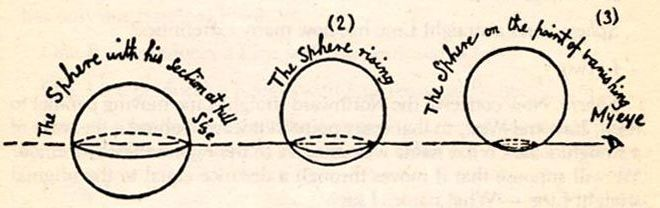
\includegraphics[width=0.9\textwidth,height=\textheight]{images/flatland-spheres.jpg}

}

\caption{\label{fig-flatland-spheres}A 2D Flatlander seeing a sphere as
it passes through Flatland. The line, labeled `My Eye' indicates what
the Flatlander would see. Source: Abbott
(\citeproc{ref-Abbott:1884}{1884})}

\end{figure}%

Abbott goes on to state what could be considered as a demonstration (or
proof) by induction of the difficulties of seeing in 1, 2, 3 dimensions,
and how the idea motion over time (one more dimension) could allow
citizens of any 1D, 2D, 3D world to contemplate one more dimension.

\begin{quote}
In One Dimensions, did not a moving Point produce a Line with two
terminal points? In two Dimensions, did not a moving Line produce a
Square with four terminal points? In Three Dimensions, did not a moving
Square produce - did not the eyes of mine behold it - that blessed
being, a Cube, with eight terminal points? And in Four Dimensions, shall
not a moving Cube - alas, for Analogy, and alas for the Progress of
Truth if it be not so - shall not, I say the motion of a divine Cube
result in a still more divine organization with sixteen terminal points?
--- Edwin A. Abbott
\end{quote}

For Abbot, the way for a citizen of any world to imagine one more
dimension was to consider how a higher-dimensional object would change
over time.\footnote{In his famous TV series, \emph{Cosmos}, Carl Sagan
  provides \href{https://youtu.be/UnURElCzGc0}{an intriguing video
  presentation} Flatland and the 4th dimension. However, as far back as
  1754 (\citeproc{ref-Cajori:1926}{Cajori, 1926}), the idea of adding a
  fourth dimension appears in Jean le Rond d'Alembert's ``Dimensions'',
  and one realization of a four-dimensional object is a
  \emph{tesseract}, shown in Figure~\ref{fig-1D-4D}.} A line moved over
time could produce a rectangle as shown in Figure~\ref{fig-1D-4D}; that
rectangle moving in another direction over time would produce a 3D
figure, and so forth.

\begin{figure}

\centering{

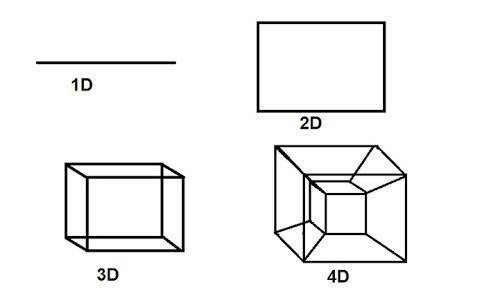
\includegraphics[width=0.9\textwidth,height=\textheight]{images/1D-4D.png}

}

\caption{\label{fig-1D-4D}Geometrical objects in 1 to 4 dimensions. One
more dimension can be thought of as the trace of movement over time.}

\end{figure}%

But wait! Where does that 4D thing (a \emph{tesseract}) come from? To
really see a tesseract it helps to view it in an animation over time
(\textbf{?@fig-tesseract}). But like the Square, contemplating 3D from a
2D world, it takes some imagination.

Yet the deep mathematics of more than three dimensions only emerged in
the 19th century. In Newtonian mechanics, space and time were always
considered independent of each other. Our familiar three-dimensional
space, of length, width, and height had formed the backbone of Euclidean
geometry for millenea. However, the idea that space and time are indeed
interwoven was first proposed by German mathematician Hermann Minkowski
(1864--1909) in 1908. This was a powerful idea. It bore fruit when
Albert Einstein revolutionized the Newtonian conceptions of gravity in
1915 when he presented a theory of general relativity which was based
primarily on the fact that mass and energy warp the fabric of
four-dimensional spacetime.

The parable of \emph{Flatland} can provide inspiration for statistical
thinking and data visualization. Once we go beyond bivariate statistics
and 2D plots, we are in a multivariate world of possibly MANY
dimensions. It takes only some imagination and suitable methods to get
there.

Like Abbott's \emph{Flatland}, this book is a romance, in many
dimensions, of what we can learn from modern methods of data
visualization.

\section*{EUREKA!}\label{eureka}
\addcontentsline{toc}{section}{EUREKA!}

\markright{EUREKA!}

Even modest sized multivariate data can have secrets that can be
revealed in the right view. As an example, David Coleman at RCA
Laboratories in Princeton, N.J. generated a dataset of five (fictitious)
measurements of grains of pollen for the 1986 Data Exposition at the
Joint statistical Meetings. The first three variables are the lengths of
geometric features 3848 observed sampled pollen grains -- in the x, y,
and z dimensions: a \texttt{ridge} along x, a \texttt{nub} in the y
direction, and a \texttt{crack} in along the z dimension. The fourth
variable is pollen grain \texttt{weight}, and the fifth is
\texttt{density}. The challenge was to ``find something interesting'' in
this dataset, now available as \texttt{animation::pollen}. \ixd{pollen}
\ixp{animation}

Those who solved the puzzle were able to find an orientation of this
5-dimensional dataset, such that zooming in revealed a magic word,
``EUREKA'' spelled in points, as in the following figure.

\begin{figure}

\begin{minipage}{0.50\linewidth}
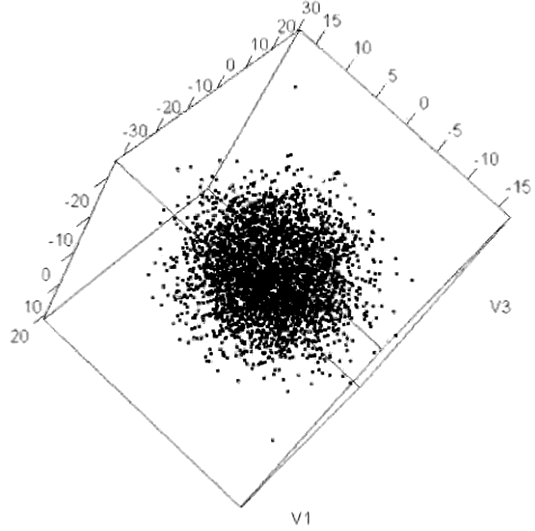
\includegraphics{images/pollen-eureka1.png}\end{minipage}%
%
\begin{minipage}{0.50\linewidth}
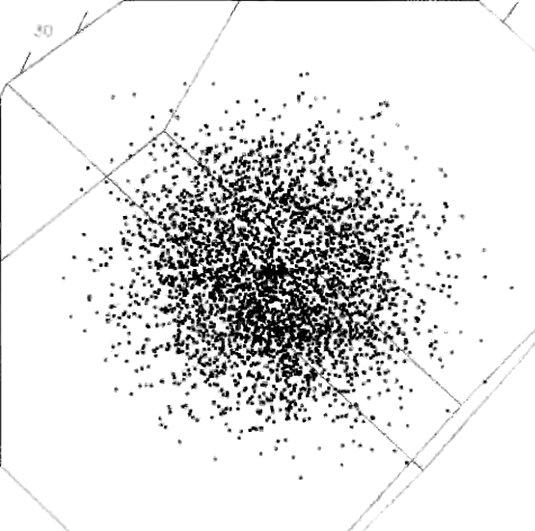
\includegraphics{images/pollen-eureka2.png}\end{minipage}%
\newline
\begin{minipage}{0.50\linewidth}
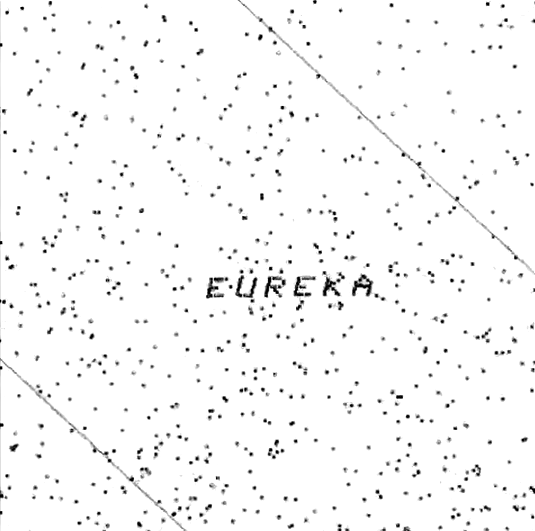
\includegraphics{images/pollen-eureka4.png}\end{minipage}%
%
\begin{minipage}{0.50\linewidth}
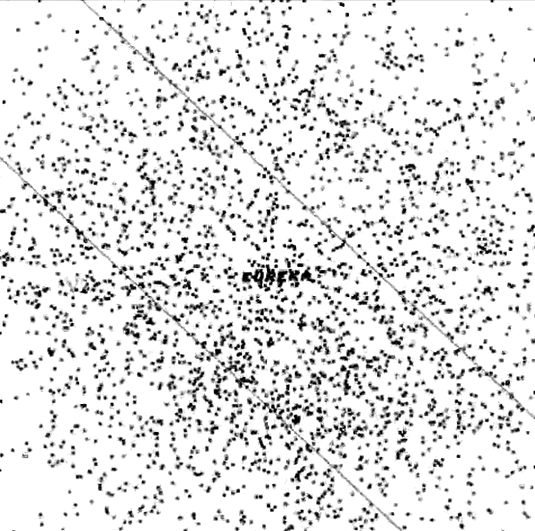
\includegraphics{images/pollen-eureka3.png}\end{minipage}%

\caption{\label{fig-pollen-eureka}Four views of the \texttt{pollen}
data, zooming in, clockwise from the upper left to discover the word
``EUREKA''.}

\end{figure}%

The path to finding the hidden word can be seen better in a 3D
animation. The online version of the book uses The \texttt{rgl} package
(\citeproc{ref-R-rgl}{Adler \& Murdoch, 2023}) create a 3D scatterplot
of the first three variables. Then the \texttt{animation} package
(\citeproc{ref-R-animation}{Xie, 2021}) is use to record a sequence of
images, adjusting the \texttt{rgl::par3d(zoom)} value. \ixp{rgl}
\ixp{animation}

\subsection*{Multivariate scientific discoveries}\label{sec-discoveries}
\addcontentsline{toc}{subsection}{Multivariate scientific discoveries}

Lest this example seem contrived (which it admittedly is), multivariate
visualization has played an important role in quite a few scientific
discoveries. Among these, Francis Galton's
(\citeproc{ref-Galton:1863}{1863}) discovery of the anti-cyclonic
pattern of wind direction in relation to barometric pressure from many
weather measures recorded systematically across all weather stations,
lighthouses and observatories in Europe in December 1861 stands out as
the best example of a scientific discovery achieved almost entirely
through graphical means---- something that was totally unexpected, and
purely the product of his use of remarkably novel high-dimensional
graphs (\citeproc{ref-FriendlyWainer:2021:TOGS}{Friendly \& Wainer,
2021, pp. 170--173}).

A more recent example is the discovery of two general classes in the
development of Type 2 diabetes by Reaven \& Miller
(\citeproc{ref-ReavenMiller:79}{1979}), using PRIM-9
(\citeproc{ref-Fishkeller-etal:1974b}{Fishkeller et al., 1974}), the
first computer system for high-dimensional visualization\footnote{PRIM-9
  is an acronym for \textbf{P}icturing, \textbf{R}otation,
  \textbf{I}solation and \textbf{M}asking in up to \textbf{9}
  dimensions. These operations are fundamental to interactive and
  dynamic data visualization.}. In an earlier study Reaven \& Miller
(\citeproc{ref-ReavenMiller:68}{1968}) examined the relation between
blood glucose levels and the production of insulin in normal subjects
and in patients with varying degrees of hyperglicemia (elevated blood
sugar level). They found a peculiar `'horse shoe'\,' shape in this
relation (shown in Figure~\ref{fig-diabetes1}), about which they could
only speculate: perhaps individuals with the best glucose tolerance also
had the lowest levels of insulin as a response to an oral dose of
glucose; perhaps those with low glucose response could secrete higher
levels of insulin; perhaps those who were low on both glucose and
insulin responses followed some other mechanism. In 2D plots, this was a
mystery.

\begin{Shaded}
\begin{Highlighting}[]
\FunctionTok{data}\NormalTok{(Diabetes, }\AttributeTok{package=}\StringTok{"heplots"}\NormalTok{)}
\FunctionTok{plot}\NormalTok{(instest }\SpecialCharTok{\textasciitilde{}}\NormalTok{ glutest, }\AttributeTok{data=}\NormalTok{Diabetes, }
     \AttributeTok{pch=}\DecValTok{16}\NormalTok{,}
     \AttributeTok{cex.lab=}\FloatTok{1.25}\NormalTok{,}
     \AttributeTok{xlab=}\StringTok{"Glucose response"}\NormalTok{,}
     \AttributeTok{ylab=}\StringTok{"Insulin response"}\NormalTok{)}
\end{Highlighting}
\end{Shaded}

\begin{figure}

\centering{

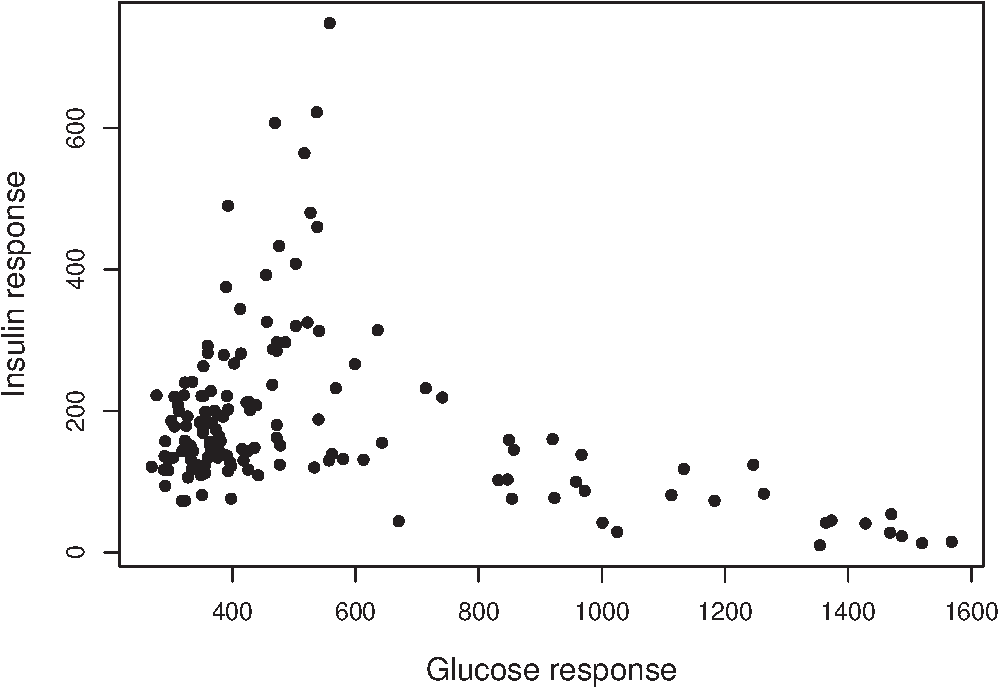
\includegraphics[width=0.7\textwidth,height=\textheight]{figs/fig-diabetes1-1.pdf}

}

\caption{\label{fig-diabetes1}Reproduction of a graph similar to that
from Reaven \& Miller (\citeproc{ref-ReavenMiller:68}{1968}) on the
relationship between glucose and insulin response to being given an oral
dose of glucose.}

\end{figure}%

An answer to their questions came ten years later, when they were able
to visualize similar but new data in 3D using the PRIM-9 system. In a
carefully controlled study, they also measured `'steady state plasma
glucose'\,' (SSPG), a measure of the efficiency of use of insulin in the
body, where large values mean insulin resistance, as well as other
variables. PRIM-9 allowed them to explore various sets of three
variables, and, more importantly, to rotate a given plot in three
dimensions to search for interesting features. One plot that stood out
concerned the relation between plasma glucose response, plasma insulin
response and SSPG response, shown in Figure~\ref{fig-ReavenMiller-3d}.

\begin{figure}

\centering{

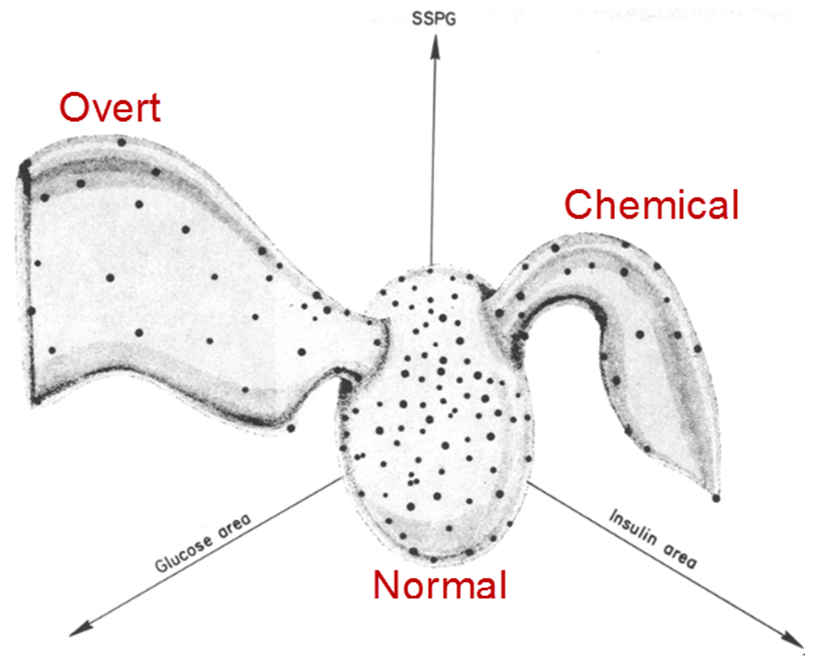
\includegraphics[width=0.7\textwidth,height=\textheight]{images/ReavenMiller-3d-annotated.png}

}

\caption{\label{fig-ReavenMiller-3d}Artist's rendition of data from
Reaven \& Miller (\citeproc{ref-ReavenMiller:79}{1979}) as seen in three
dimensions using the PRIM-9 system. Labels for the clusters have been
added, identifying the three groups of patients. \emph{Source}: Reaven
\& Miller (\citeproc{ref-ReavenMiller:79}{1979}).}

\end{figure}%

From this graphical insight, they were able to classify the participants
into three groups, based on clinical levels of glucose and insulin. The
people in the wing on the left in Figure~\ref{fig-ReavenMiller-3d} were
considered to have overt diabetes, the most advanced form, characterized
by elevated fasting blood glucose concentration and classical diabetic
symptoms. Those in the right wing were classified as latent or chemical
diabetics, with no symptoms of diabetes but demonstrable abnormality of
oral or intravenous glucose tolerance. Those in the central blob were
classified as normal.

Previous thinking was that Type 2 diabetes (when the body cannot make
\emph{enough} insulin, as opposed to Type I, an autoimmune condition
where the pancreatic cells have been destroyed) progressed from the
chemical stage to an overt one in a smooth transition. However, it was
clear from Figure~\ref{fig-ReavenMiller-3d} that the only ``path'' from
one to the other lead through the cluster of normal patients near the
origin, so that explanation must be wrong. Instead, this suggested that
the chemical and overt diabetics were distinct classes. Indeed,
longitudinal studies showed that patients classified as chemical
diabetics rarely developed the overt form. The understanding of the
etiology of Type 2 diabetes was altered dramatically by the power of
high-D interactive graphics.

\section*{What I assume}\label{what-i-assume}
\addcontentsline{toc}{section}{What I assume}

\markright{What I assume}

It is assumed that the reader has a background in applied
\emph{intermediate} statistics including material on univariate linear
models including analysis of variance (ANOVA) and multiple regression.
This means you should be familiar with \ldots{} \textbf{TODO}: Complete
this required background

There will also be some mathematics in the book where words and diagrams
are not enough. The mathematical level will be intermediate, mostly
consisting of simple algebra. No derivations, proofs, theorems here! For
multivariate methods, it will be useful to express ideas using matrix
notation to simplify presentation. The single symbol I'm using math to
express ideas, and all you will need is a reading-level of
understanding. For this, the first chapter of Fox
(\citeproc{ref-Fox2021}{2021}), \emph{A mathematical primer for social
statistics}, is excellent. If you want to learn something of using
matrix algebra for data analysis and statistics, I recommend our package
\texttt{matlib} (\citeproc{ref-R-matlib}{Friendly et al., 2024}).

I also assume the reader to have at least a basic familiarity with R.
While R fundamentals are outside the scope of the book, I believe that
this language provides a rich set of resources, far beyond that offered
by other statistical software packages, and is well worth learning.

For those not familiar with R, I recommend Matloff
(\citeproc{ref-Matloff-2011}{2011}), Wickham
(\citeproc{ref-Wickham2014}{2014}), and Cotton
(\citeproc{ref-Cotton-2013}{2013}) for introductions to programming in
the language. Fox \& Weisberg (\citeproc{ref-FoxWeisberg:2018}{2018a})
and Teetor (\citeproc{ref-Teetor2011}{2011}) are great for learning
about how to conduct basic statistical analyses in R. \textbf{TODO}:
Revise this list.

\section*{Conventions used in this
book}\label{conventions-used-in-this-book}
\addcontentsline{toc}{section}{Conventions used in this book}

\markright{Conventions used in this book}

The following typographic conventions are used in this book:

\begin{itemize}
\item
  \emph{italic} : indicates terms to be \emph{emphasized} or defined in
  the text, \ldots{}
\item
  \textbf{bold} : is used for names of R packages. Or, better yet:
  \textbf{\texttt{bold\ monospace}}, but I'd rather this be in a
  \textcolor{darkgreen}{different color}. Perhaps I can use ``r
  colorize(''\textbf{lattice}'', ``green'')'' inline -\textgreater{}
  \textcolor{green}{**lattice**} will do this? This does bold \& color,
  but can't use monospace.

  I can now use inline `pkg(``lattice'')' generating \texttt{lattice},
  or also with a citation, \texttt{pkg("lattice",\ cite=TRUE)}
  -\textgreater{} \texttt{lattice} (\citeproc{ref-R-lattice}{Sarkar,
  2024}), but can't do color or monospace with this.
\item
  \texttt{fixed-width} : is used in program listings as well as in text
  to refer to variable and function names, R statement elements and
  keywords.
\item
  R code in program listings and output is presented in
  \texttt{monospaced\ (typewriter)} font,
  \href{https://fonts.google.com/specimen/Fira+Mono}{\texttt{fira\ mono}}
\item
  \emph{\texttt{fixed-width\ italic}} : isn't used yet, but probably
  should be.
\end{itemize}

For R functions in packages, we use the notation
\texttt{package::function()}, for example: \texttt{car::Anova()} to
identify where those functions are defined

\mainmatter

\part{Orienting Ideas}

\chapter{Introduction}\label{sec-introduction}

This material may or may not survive; it was taken from an earlier
article.

\section{Multivariate vs.~multivariable
methods}\label{multivariate-vs.-multivariable-methods}

\begin{quote}
multivariate \(\ne\) multivariable
\end{quote}

In this era of multivitamins, multitools, multifactor authentication and
even the multiverse, it is well to understand the distinction between
\emph{multivariate} and \emph{multivariable} methods as these terms are
generally used and as I use them here in relation to statistical methods
and data visualization. The distinction is simple:

\begin{itemize}
\item
  \textbf{Multivariate methods} for linear models such as multivariate
  regression have more than one dependent, response or outcome variable.
  Other multivariate methods such as principal components analysis or
  factor analysis treat all variables on an equal footing.
\item
  \textbf{Multivariable methods} have a single dependent variable and
  more than one independent variables or covariates.
\end{itemize}

\section{Why use a multivariate
design}\label{why-use-a-multivariate-design}

A particular research outcome (e.g., depression, neuro-cognitive
functioning, academic achievement, self-concept, attention deficit
hyperactivity disorders) might take on a multivariate form if it has
several observed measurement scales or related aspects by which it is
quantified, or if there are multiple theoretically distinct outcomes
that should be assessed in conjunction with each other (e.g., using
depression, generalized anxiety, and stress inventories to model overall
happiness). In this situation, the primary concern of the researcher is
to ascertain the impact of potential predictors on two or more response
variables simultaneously.

For example, if academic achievement is measured for adolescents by
their reading, mathematics, science, and history scores, the following
questions are of interest:

\begin{itemize}
\item
  Do predictors such as parent encouragement, socioeconomic status and
  school environmental variables affect \emph{all} of these outcomes?
\item
  Do they affect them in the \emph{same} or \emph{different} ways?
\item
  How many different aspects of academic achievement can be
  distinguished in the predictors? Equivalently, is academic achievement
  \emph{unidimensional} or \emph{multidimensional} in relation to the
  predictors?
\end{itemize}

Similarly, if psychiatric patients in various diagnostic categories are
measured on a battery of tests related to social skills and cognitive
functioning, we might want to know:

\begin{itemize}
\item
  Which measures best discriminate among the diagnostic groups?
\item
  Which measures are most predictive of positive outcomes?
\item
  Further, how are the \emph{relationships} between the outcomes
  affected by the predictors?
\end{itemize}

Such questions obviously concern more than just the separate univariate
relations of each response to the predictors. Equally, or perhaps more
importantly, are questions of how the response variables are predicted
\emph{jointly}.

\begin{tcolorbox}[enhanced jigsaw, breakable, left=2mm, bottomtitle=1mm, arc=.35mm, colframe=quarto-callout-note-color-frame, coltitle=black, title=\textcolor{quarto-callout-note-color}{\faInfo}\hspace{0.5em}{SEM}, colback=white, toptitle=1mm, rightrule=.15mm, opacityback=0, colbacktitle=quarto-callout-note-color!10!white, titlerule=0mm, leftrule=.75mm, toprule=.15mm, bottomrule=.15mm, opacitybacktitle=0.6]

Structural equation modeling (SEM) offers another route to explore and
analyze the relationships among multiple predictors and multiple
responses. They have the advantage of being able to test potentially
complex systems of linear equations in very flexible ways; however,
these methods are often far removed from data analysis \emph{per se} and
except for path diagrams offer little in the way of visualization
methods to aid in understanding and communicating the results. The
graphical methods we describe here can also be useful in a SEM context.
\ix{Structural equation model}

\end{tcolorbox}

\section{Linear models: Univariate to
multivariate}\label{linear-models-univariate-to-multivariate}

For classical linear models for ANOVA and regression, the step from a
univariate model for a single response, \(y\), to a multivariate one for
a collection of \(p\) responses, \(\mathbf{y}\) is conceptually very
easy. That's because the univariate model,

\[y_i = \beta_0 + \beta_1 x_1 + \beta_2 x_2 + \dots + \beta_q x_q + \epsilon_i , \]

or, in matrix terms,

\[\mathbf{y} = \mathbf{X} \; \mathbf{\beta} + \mathbf{\epsilon}, \quad\mbox{   with   }\quad \mathbf{u} \sim \mathcal{N} (0, \sigma^2 \mathbf{I}) ,\]

generalizes directly to an analogous multivariate linear model (MLM),

\[\mathbf{Y} = [\mathbf{y_1}, \mathbf{y_2}, \dots, \mathbf{y_p}] = \mathbf{X} \; \mathbf{B} + \Epsilon \quad\mbox{   with   }\quad \Epsilon \sim \mathcal{N} (\mathbf{0}, \mathbf{\Sigma})\]

for multiple responses (as will be discussed in detail). The design
matrix, \(\mathbf{X}\) remains the same, and the vector \(\beta\) of
coefficients becomes a matrix \(\mathbf{B}\), with one column for each
of the \(p\) outcome variables.

Happily as well, hypothesis tests for the MLM are also straight-forward
generalizations of the familiar \(F\) and \(t\)-tests for univariate
response models. Moreover, there is a rich geometry underlying these
generalizations which we can exploit for understanding and
visualization.

\section{Visualization is harder}\label{visualization-is-harder}

However, with two or more response variables, visualizations for
multivariate models are not as simple as they are for their univariate
counterparts for understanding the effects of predictors, model
parameters, or model diagnostics. Consequently, the results of such
studies are often explored and discussed solely in terms of coefficients
and significance, and visualizations of the relationships are only
provided for one response variable at a time, if at all. This tradition
can mask important nuances, and lead researchers to draw erroneous
conclusions.

The aim of this book is to describe and illustrate some central methods
that we have developed over the last ten years that aid in the
understanding and communication of the results of multivariate linear
models (\citeproc{ref-Friendly-07-manova}{Friendly, 2007};
\citeproc{ref-FriendlyMeyer:2016:DDAR}{Friendly \& Meyer, 2016}). These
methods rely on \emph{data ellipsoids} as simple, minimally sufficient
visualizations of variance that can be shown in 2D and 3D plots. As will
be demonstrated, the \emph{Hypothesis-Error (HE) plot} framework applies
this idea to the results of multivariate tests of linear hypotheses.
\ix{data ellipse} \ix{HE plot}

Further, in the case where there are more than just a few outcome
variables, the important nectar of their relationships to predictors can
often be distilled in a multivariate juicer--- a \textbf{projection} of
the multivariate relationships to the predictors in the low-D space that
captures most of the flavor. This idea can be applied using
\emph{canonical correlation plots} and with \emph{canonical discriminant
HE plots}. \ix{canonical correlation} \ix{projection}

\begin{figure}[H]

{\centering 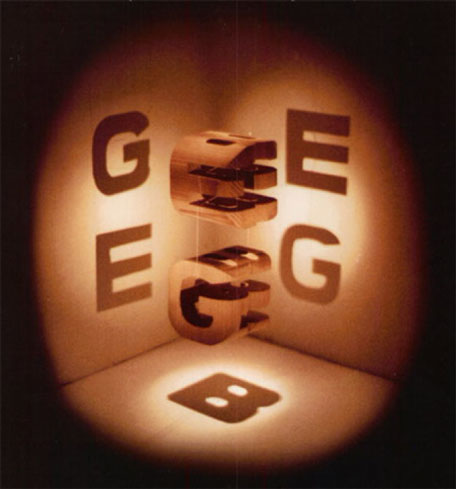
\includegraphics{images/Cover-GBE.png}

}

\caption{\textbf{Projection}: The cover image from Hofstadter's
\emph{Gödel, Bach and Escher} illustrates projection of 3D solids onto
each 2D plane.}

\end{figure}%

\section{Problems in understanding and communicating MLM
results}\label{sec-problems}

In my consulting practice within the Statistical Consulting Service at
York University, I see hundreds of clients each year ranging from
advanced undergraduate thesis students, to graduate students and faculty
from a variety of fields. Over the last two decades, and across each of
these groups, I have noticed an increasing desire to utilize
multivariate methods. As researchers are exposed to the utility and
power of multivariate tests, they see them as an appealing alternative
to running many univariate ANOVAs or multiple regressions for each
response variable separately.

However, multivariate analyses are more complicated than such
approaches, especially when it comes to understanding and communicating
results. Output is typically voluminous, and researchers will often get
lost in the numbers. While software (SPSS, SAS and R) make tabular
summary displays easy, these often obscure the findings that researchers
are most interested in. The most common analytic oversights that we have
observed are:

\begin{itemize}
\item
  \textbf{Atomistic data screening}: Researchers have mostly learned the
  assumptions (the Holy Trinity of normality, constant variance and
  independence) of univariate linear models, but then apply
  \emph{univariate} tests (e.g., Shapiro-Wilk) and diagnostic plots
  (normal QQ plots) to every predictor and every response.
\item
  \textbf{Bonferroni everywhere}: Faced with the task of reporting the
  results for multiple response measures and a collection of predictors
  for each, a common tendency is to run (and sometimes report) each of
  the separate univariate response models and then apply a correction
  for multiple testing. Not only is this confusing and awkward to
  report, but it is largely unnecessary because the multivariate tests
  provide protection for multiple testing.
\item
  \textbf{Reverting to univariate visualizations}: To display results,
  SPSS and SAS make some visualization methods available through menu
  choices or syntax, but usually these are the wrong (or at least
  unhelpful) choices, in that they generate separate univariate graphs
  for the individual responses.
\end{itemize}

This book to discusses a few essential procedures for multivariate
linear models, how their interpretation can be aided through the use of
well-crafted (though novel) visualizations, and provides replicable
sample code in R to showcase their use in applied behaviorial research.
A later section {[}ref?{]} provides some practical guidelines for
analyzing, visualizing and reporting such models to help avoid these and
other problems.

\textbf{Package summary}:

1 packages used here: knitr

\chapter{Getting Started}\label{sec-getting_started}

\section{Why plot your data?}\label{sec-why_plot}

\begin{quote}
Getting information from a table is like extracting sunlight from a
cucumber. Farquhar \& Farquhar
(\citeproc{ref-FarquharFarquhar:91}{1891})
\end{quote}

At the time the Farhquhar brothers wrote this pithy aphorism, graphical
methods for understanding data had advanced considerably, but were not
universally practiced, prompting their complaint.

The main graphic forms we use today---the pie chart, line graphs and
bar---were invented by William Playfair around 1800
(\citeproc{ref-Playfair:1786}{Playfair, 1786},
\citeproc{ref-Playfair:1801}{1801}). The scatterplot arrived shortly
after (\citeproc{ref-Herschel:1833}{Herschel, 1833}) and thematic maps
showing the spatial distributions of social variables (crime, suicides,
literacy) were used for the first time to reason about important
societal questions (\citeproc{ref-Guerry:1833}{Guerry, 1833}) such as
``is increased education associated with lower rates of crime?''
\ix{pie chart} \ix{bar chart} \ix{line graph} \ix{scatterplot}

In the last half of the 18th Century, the idea of correlation was
developed (\citeproc{ref-Galton:1886}{Galton, 1886};
\citeproc{ref-Pearson:1896}{Pearson, 1896}) and the period, roughly
1860--1890, dubbed the ``Golden Age of Graphics
(\citeproc{ref-Funkhouser:1937}{Funkhouser, 1937}) became the richest
period of innovation and beauty in the entire history of data
visualization. During this time there was an incredible development of
visual thinking, represented by the work of Charles Joseph Minard,
advances in the role of visualization within scientific discovery, as
illustrated through Francis Galton, and graphical excellence, embodied
in state statistical atlases produced in France and elsewhere. See
Friendly (\citeproc{ref-Friendly:2008:golden}{2008}); Friendly \& Wainer
(\citeproc{ref-FriendlyWainer:2021:TOGS}{2021}) for this history.

\subsection{Anscombe's Quartet}\label{sec-anscombe}

In 1973, Francis Anscombe (\citeproc{ref-Anscombe:73}{Anscombe, 1973})
famously constructed a set of four datasets illustrate the importance of
plotting the graphs before analyzing and model building, and the effect
of unusual observations on fitted models. Now known as \emph{Anscombe's
Quartet}, these datasets had identical statistical properties: the same
means, standard devitions, correlations and regression lines.

His purpose was to debunk three notions that had been prevalent at the
time:

\begin{itemize}
\tightlist
\item
  Numerical calculations are exact, but graphs are coarse and limited by
  perception and resolution;
\item
  For any particular kind of statistical data there is just one set of
  calculations constituting a correct statistical analysis;
\item
  Performing intricate calculations is virtuous, whereas actually
  looking at the data is cheating.
\end{itemize}

The dataset \texttt{datasets::anscombe} has 11 observations, recorded in
wide format, with variables \texttt{x1:x4} and \texttt{y1:y4}.

\begin{Shaded}
\begin{Highlighting}[]
\FunctionTok{data}\NormalTok{(anscombe) }
\FunctionTok{head}\NormalTok{(anscombe)}
\CommentTok{\#\textgreater{}   x1 x2 x3 x4   y1   y2    y3   y4}
\CommentTok{\#\textgreater{} 1 10 10 10  8 8.04 9.14  7.46 6.58}
\CommentTok{\#\textgreater{} 2  8  8  8  8 6.95 8.14  6.77 5.76}
\CommentTok{\#\textgreater{} 3 13 13 13  8 7.58 8.74 12.74 7.71}
\CommentTok{\#\textgreater{} 4  9  9  9  8 8.81 8.77  7.11 8.84}
\CommentTok{\#\textgreater{} 5 11 11 11  8 8.33 9.26  7.81 8.47}
\CommentTok{\#\textgreater{} 6 14 14 14  8 9.96 8.10  8.84 7.04}
\end{Highlighting}
\end{Shaded}

The following code transforms this data to long format and calculates
some summary statistics for each \texttt{dataset}.

\begin{Shaded}
\begin{Highlighting}[]
\NormalTok{anscombe\_long }\OtherTok{\textless{}{-}}\NormalTok{ anscombe }\SpecialCharTok{|\textgreater{}} 
  \FunctionTok{pivot\_longer}\NormalTok{(}\FunctionTok{everything}\NormalTok{(), }
               \AttributeTok{names\_to =} \FunctionTok{c}\NormalTok{(}\StringTok{".value"}\NormalTok{, }\StringTok{"dataset"}\NormalTok{), }
               \AttributeTok{names\_pattern =} \StringTok{"(.)(.)"}
\NormalTok{  ) }\SpecialCharTok{|\textgreater{}}
  \FunctionTok{arrange}\NormalTok{(dataset)}

\NormalTok{anscombe\_long }\SpecialCharTok{|\textgreater{}}
  \FunctionTok{group\_by}\NormalTok{(dataset) }\SpecialCharTok{|\textgreater{}}
  \FunctionTok{summarise}\NormalTok{(}\AttributeTok{xbar      =} \FunctionTok{mean}\NormalTok{(x),}
            \AttributeTok{ybar      =} \FunctionTok{mean}\NormalTok{(y),}
            \AttributeTok{r         =} \FunctionTok{cor}\NormalTok{(x, y),}
            \AttributeTok{intercept =} \FunctionTok{coef}\NormalTok{(}\FunctionTok{lm}\NormalTok{(y }\SpecialCharTok{\textasciitilde{}}\NormalTok{ x))[}\DecValTok{1}\NormalTok{],}
            \AttributeTok{slope     =} \FunctionTok{coef}\NormalTok{(}\FunctionTok{lm}\NormalTok{(y }\SpecialCharTok{\textasciitilde{}}\NormalTok{ x))[}\DecValTok{2}\NormalTok{]}
\NormalTok{         )}
\CommentTok{\#\textgreater{} \# A tibble: 4 x 6}
\CommentTok{\#\textgreater{}   dataset  xbar  ybar     r intercept slope}
\CommentTok{\#\textgreater{}   \textless{}chr\textgreater{}   \textless{}dbl\textgreater{} \textless{}dbl\textgreater{} \textless{}dbl\textgreater{}     \textless{}dbl\textgreater{} \textless{}dbl\textgreater{}}
\CommentTok{\#\textgreater{} 1 1           9  7.50 0.816      3.00 0.500}
\CommentTok{\#\textgreater{} 2 2           9  7.50 0.816      3.00 0.5  }
\CommentTok{\#\textgreater{} 3 3           9  7.5  0.816      3.00 0.500}
\CommentTok{\#\textgreater{} 4 4           9  7.50 0.817      3.00 0.500}
\end{Highlighting}
\end{Shaded}

As we can see, all four datasets have nearly identical univariate and
bivariate statistical measures. You can only see how they differ in
graphs, which show their true natures to be vastly different.

Figure~\ref{fig-ch02-anscombe1} is an enhanced version of Anscombe's
plot of these data, adding helpful annotations to show visually the
underlying statistical summaries.

\begin{figure}

\centering{

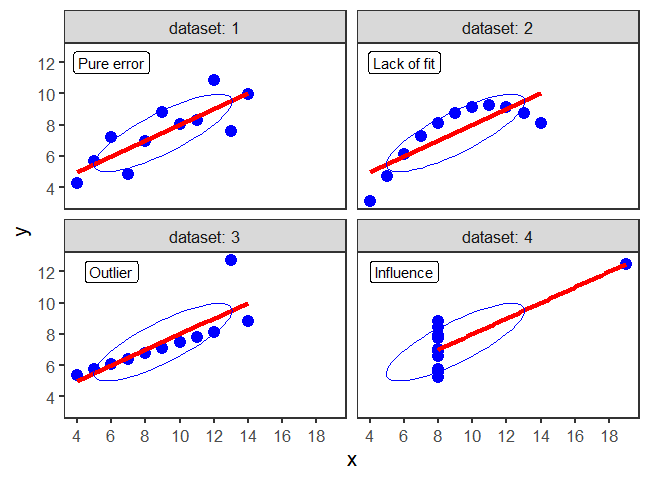
\includegraphics[width=0.9\textwidth,height=\textheight]{figs/ch02/ch02-anscombe1.png}

}

\caption{\label{fig-ch02-anscombe1}Scatterplots of Anscombe's Quartet.
Each plot shows the fitted regression line and a 68\% data ellipse
representing the correlation between \(x\) and \(y\).}

\end{figure}%

This figure is produced as follows, using a single call to
\texttt{ggplot()}, faceted by \texttt{dataset}. As we will see later
(Section~\ref{sec-data-ellipse}), the data ellipse (produced by
\texttt{stat\_ellipse()}) reflects the correlation between the
variables.

\begin{Shaded}
\begin{Highlighting}[]
\NormalTok{desc }\OtherTok{\textless{}{-}} \FunctionTok{tibble}\NormalTok{(}
  \AttributeTok{dataset =} \DecValTok{1}\SpecialCharTok{:}\DecValTok{4}\NormalTok{,}
  \AttributeTok{label =} \FunctionTok{c}\NormalTok{(}\StringTok{"Pure error"}\NormalTok{, }\StringTok{"Lack of fit"}\NormalTok{, }\StringTok{"Outlier"}\NormalTok{, }\StringTok{"Influence"}\NormalTok{)}
\NormalTok{)}

\FunctionTok{ggplot}\NormalTok{(anscombe\_long, }\FunctionTok{aes}\NormalTok{(}\AttributeTok{x =}\NormalTok{ x, }\AttributeTok{y =}\NormalTok{ y)) }\SpecialCharTok{+}
  \FunctionTok{geom\_point}\NormalTok{(}\AttributeTok{color =} \StringTok{"blue"}\NormalTok{, }\AttributeTok{size =} \DecValTok{4}\NormalTok{) }\SpecialCharTok{+}
  \FunctionTok{geom\_smooth}\NormalTok{(}\AttributeTok{method =} \StringTok{"lm"}\NormalTok{, }\AttributeTok{formula =}\NormalTok{ y }\SpecialCharTok{\textasciitilde{}}\NormalTok{ x, }\AttributeTok{se =} \ConstantTok{FALSE}\NormalTok{,}
              \AttributeTok{color =} \StringTok{"red"}\NormalTok{, }\AttributeTok{linewidth =} \FloatTok{1.5}\NormalTok{) }\SpecialCharTok{+}
  \FunctionTok{scale\_x\_continuous}\NormalTok{(}\AttributeTok{breaks =} \FunctionTok{seq}\NormalTok{(}\DecValTok{0}\NormalTok{,}\DecValTok{20}\NormalTok{,}\DecValTok{2}\NormalTok{)) }\SpecialCharTok{+}
  \FunctionTok{scale\_y\_continuous}\NormalTok{(}\AttributeTok{breaks =} \FunctionTok{seq}\NormalTok{(}\DecValTok{0}\NormalTok{,}\DecValTok{12}\NormalTok{,}\DecValTok{2}\NormalTok{)) }\SpecialCharTok{+}
  \FunctionTok{stat\_ellipse}\NormalTok{(}\AttributeTok{level =} \FloatTok{0.5}\NormalTok{, }\AttributeTok{color=}\NormalTok{col, }\AttributeTok{type=}\StringTok{"norm"}\NormalTok{) }\SpecialCharTok{+}
  \FunctionTok{geom\_label}\NormalTok{(}\AttributeTok{data=}\NormalTok{desc, }\FunctionTok{aes}\NormalTok{(}\AttributeTok{label =}\NormalTok{ label), }\AttributeTok{x=}\DecValTok{6}\NormalTok{, }\AttributeTok{y=}\DecValTok{12}\NormalTok{) }\SpecialCharTok{+}
  \FunctionTok{facet\_wrap}\NormalTok{(}\SpecialCharTok{\textasciitilde{}}\NormalTok{dataset, }\AttributeTok{labeller =}\NormalTok{ label\_both) }
\end{Highlighting}
\end{Shaded}

The subplots are labeled with the statistical idea they reflect:

\begin{itemize}
\item
  dataset 1: \textbf{Pure error}. This is the typical case with
  well-behaved data. Variation of the points around the line reflect
  only measurement error or unreliability in the response, \(y\).
\item
  dataset 2: \textbf{Lack of fit}. The data is clearly curvilinear, and
  would be very well described by a quadratic,
  \texttt{y\ \textasciitilde{}\ poly(x,\ 2)}. This violates the
  assumption of linear regression that the fitted model has the correct
  form.
\item
  dataset 3: \textbf{Outlier}. One point, second from the right, has a
  very large residual. Because this point is near the extreme of \(x\),
  it pulls the regression line towards it, as you can see by imagining a
  line through the remaining points.
\item
  dataset 4: \textbf{Influence}. All but one of the points have the same
  \(x\) value. The one unusual point has sufficient influence to force
  the regression line to fit it \textbf{exactly}.
\end{itemize}

One moral from this example:

\begin{quote}
\textbf{Linear regression only ``sees'' a line. It does its' best when
the data are really linear. Because the line is fit by least squares, it
pulls the line toward discrepant points to minimize the sum of squared
residuals.}
\end{quote}

\begin{tcolorbox}[enhanced jigsaw, breakable, left=2mm, bottomtitle=1mm, arc=.35mm, colframe=quarto-callout-note-color-frame, coltitle=black, title=\textcolor{quarto-callout-note-color}{\faInfo}\hspace{0.5em}{Datasaurus Dozen}, colback=white, toptitle=1mm, rightrule=.15mm, opacityback=0, colbacktitle=quarto-callout-note-color!10!white, titlerule=0mm, leftrule=.75mm, toprule=.15mm, bottomrule=.15mm, opacitybacktitle=0.6]

The method Anscombe used to compose his quartet is unknown, but it turns
out that that there is a method to construct a wider collection of
datasets with identical statistical properties. After all, in a
bivariate dataset with \(n\) observations, the correlation has \((n-2)\)
degrees of freedom, so it is possible to choose \(n-2\) of the
\((x, y)\) pairs to yield any given value. As it happens, it is also
possible to create any number of datasets with the same means, standard
deviations and correlations with nearly any shape you like --- even a
dinosaur!

The \emph{Datasaurus Dozen} was first publicized by Alberto Cairo in a
\href{http://www.thefunctionalart.com/2016/08/download-datasaurus-never-trust-summary.html}{blog
post} and are available in the \textbf{datasauRus} package Davies et al.
(\citeproc{ref-R-datasauRus}{2022}). As shown in
\textbf{?@fig-datasaurus}, the sets include a star, cross, circle,
bullseye, horizontal and vertical lines, and, of course the ``dino''.
The method (\citeproc{ref-MatejkaFitzmaurice2017}{Matejka \&
Fitzmaurice, 2017}) uses \emph{simulated annealing}, an iterative
process that perturbs the points in a scatterplot, moving them towards a
given shape while keeping the statistical summaries close to the fixed
target value.

The \textbf{datasauRus} package just contains the datasets, but a
general method, called \emph{statistical metamers}, for producing such
datasets has been described by
\href{https://eliocamp.github.io/codigo-r/en/2019/01/statistical-metamerism/}{Elio
Campitelli} and implemented in the \textbf{metamer} package.

\end{tcolorbox}

\begin{tcolorbox}[enhanced jigsaw, breakable, left=2mm, bottomtitle=1mm, arc=.35mm, colframe=quarto-callout-note-color-frame, coltitle=black, title=\textcolor{quarto-callout-note-color}{\faInfo}\hspace{0.5em}{Quartets}, colback=white, toptitle=1mm, rightrule=.15mm, opacityback=0, colbacktitle=quarto-callout-note-color!10!white, titlerule=0mm, leftrule=.75mm, toprule=.15mm, bottomrule=.15mm, opacitybacktitle=0.6]

The essential idea of a statistical ``quartet'' is to illustrate four
quite different datasets or circumstances that seem superficially the
same, but yet are paradoxically very different when you look behind the
scenes. For example, in the context of causal analysis Gelman et al.
(\citeproc{ref-Gelman-etal:2023}{2023}), illustrated sets of four
graphs, within each of which all four represent the same average
(latent) causal effect but with much different patterns of individual
effects; McGowan et al. (\citeproc{ref-McGowan2023}{2023}) provide
another illustration with four seemingly identical data sets each
generated by a different causal mechanism. As an example of machine
learning models, Biecek et al. (\citeproc{ref-Biecek-etal:2023}{2023}),
introduced the ``Rashamon Quartet'', a synthetic dataset for which four
models from different classes (linear model, regression tree, random
forest, neural network) have practically identical predictive
performance. In all cases, the paradox is solved when their
visualization reveals the distinct ways of understanding structure in
the data. The
\href{https://r-causal.github.io/quartets/}{\textbf{quartets}} package
contains these and other variations on this theme.

\end{tcolorbox}

\subsection{A real example}\label{sec-davis}

In the mid 1980s, a consulting client had a strange problem. She was
conducting a study of the relation between body image and weight
preoccupation in exercising and non-exercising people
(\citeproc{ref-Davis:1990}{Davis, 1990}). As part of the design, the
researcher wanted to know if self-reported weight could be taken as a
reliable indicator of true weight measured on a scale. It was expected
that the correlations between reported and measured weight should be
close to 1.0, and the slope of the regression lines for men and women
should also be close to 1.0. The dataset is \texttt{car::Davis}.

She was therefore very surprise to see the following numerical results:
For men, the correlation was nearly perfect, but not so for women.

\begin{Shaded}
\begin{Highlighting}[]
\FunctionTok{data}\NormalTok{(Davis, }\AttributeTok{package=}\StringTok{"carData"}\NormalTok{)}
\NormalTok{Davis }\OtherTok{\textless{}{-}}\NormalTok{ Davis }\SpecialCharTok{|\textgreater{}}
  \FunctionTok{drop\_na}\NormalTok{()          }\CommentTok{\# drop missing cases}
\NormalTok{Davis }\SpecialCharTok{|\textgreater{}}
  \FunctionTok{group\_by}\NormalTok{(sex) }\SpecialCharTok{|\textgreater{}}
  \FunctionTok{select}\NormalTok{(sex, weight, repwt) }\SpecialCharTok{|\textgreater{}}
  \FunctionTok{summarise}\NormalTok{(}\AttributeTok{r =} \FunctionTok{cor}\NormalTok{(weight, repwt))}
\CommentTok{\#\textgreater{} \# A tibble: 2 x 2}
\CommentTok{\#\textgreater{}   sex       r}
\CommentTok{\#\textgreater{}   \textless{}fct\textgreater{} \textless{}dbl\textgreater{}}
\CommentTok{\#\textgreater{} 1 F     0.501}
\CommentTok{\#\textgreater{} 2 M     0.979}
\end{Highlighting}
\end{Shaded}

Similarly, the regression lines showed the expected slope for men, but
that for women was only 0.26.

\begin{Shaded}
\begin{Highlighting}[]
\NormalTok{Davis }\SpecialCharTok{|\textgreater{}}
  \FunctionTok{nest}\NormalTok{(}\AttributeTok{data =} \SpecialCharTok{{-}}\NormalTok{sex) }\SpecialCharTok{|\textgreater{}}
  \FunctionTok{mutate}\NormalTok{(}\AttributeTok{model =} \FunctionTok{map}\NormalTok{(data, }\SpecialCharTok{\textasciitilde{}} \FunctionTok{lm}\NormalTok{(repwt }\SpecialCharTok{\textasciitilde{}}\NormalTok{ weight, }\AttributeTok{data =}\NormalTok{ .)),}
         \AttributeTok{tidied =} \FunctionTok{map}\NormalTok{(model, tidy)) }\SpecialCharTok{|\textgreater{}}
  \FunctionTok{unnest}\NormalTok{(tidied) }\SpecialCharTok{|\textgreater{}}
  \FunctionTok{filter}\NormalTok{(term }\SpecialCharTok{==} \StringTok{"weight"}\NormalTok{) }\SpecialCharTok{|\textgreater{}}
  \FunctionTok{select}\NormalTok{(sex, term, estimate, std.error)}
\CommentTok{\#\textgreater{} \# A tibble: 2 x 4}
\CommentTok{\#\textgreater{}   sex   term   estimate std.error}
\CommentTok{\#\textgreater{}   \textless{}fct\textgreater{} \textless{}chr\textgreater{}     \textless{}dbl\textgreater{}     \textless{}dbl\textgreater{}}
\CommentTok{\#\textgreater{} 1 M     weight    0.990    0.0229}
\CommentTok{\#\textgreater{} 2 F     weight    0.262    0.0459}
\end{Highlighting}
\end{Shaded}

``What could be wrong here?'', the client asked. The consultant replied
with the obvious question:

\begin{quote}
\emph{Did you plot your data?}
\end{quote}

The answer turned out to be one discrepant point, a female, whose
measured weight was 166 kg (366 lbs!). This single point exerted so much
influence that it pulled the fitted regression line down to a slope of
only 0.26.

\begin{Shaded}
\begin{Highlighting}[]
\CommentTok{\# shorthand to position legend inside the figure}
\NormalTok{legend\_inside }\OtherTok{\textless{}{-}} \ControlFlowTok{function}\NormalTok{(position) \{}
  \FunctionTok{theme}\NormalTok{(}\AttributeTok{legend.position =} \StringTok{"inside"}\NormalTok{,}
        \AttributeTok{legend.position.inside =}\NormalTok{ position)}
\NormalTok{\}}

\NormalTok{Davis }\SpecialCharTok{|\textgreater{}}
  \FunctionTok{ggplot}\NormalTok{(}\FunctionTok{aes}\NormalTok{(}\AttributeTok{x =}\NormalTok{ weight, }\AttributeTok{y =}\NormalTok{ repwt, }
             \AttributeTok{color =}\NormalTok{ sex, }\AttributeTok{shape =}\NormalTok{ sex, }\AttributeTok{linetype =}\NormalTok{ sex)) }\SpecialCharTok{+}
  \FunctionTok{geom\_point}\NormalTok{(}\AttributeTok{size =} \FunctionTok{ifelse}\NormalTok{(Davis}\SpecialCharTok{$}\NormalTok{weight}\SpecialCharTok{==}\DecValTok{166}\NormalTok{, }\DecValTok{6}\NormalTok{, }\DecValTok{2}\NormalTok{)) }\SpecialCharTok{+}
  \FunctionTok{geom\_smooth}\NormalTok{(}\AttributeTok{method =} \StringTok{"lm"}\NormalTok{, }\AttributeTok{formula =}\NormalTok{ y}\SpecialCharTok{\textasciitilde{}}\NormalTok{x, }\AttributeTok{se =} \ConstantTok{FALSE}\NormalTok{) }\SpecialCharTok{+}
  \FunctionTok{labs}\NormalTok{(}\AttributeTok{x =} \StringTok{"Measured weight (kg)"}\NormalTok{, }\AttributeTok{y =} \StringTok{"Reported weight (kg)"}\NormalTok{) }\SpecialCharTok{+}
  \FunctionTok{scale\_linetype\_manual}\NormalTok{(}\AttributeTok{values =} \FunctionTok{c}\NormalTok{(}\AttributeTok{F =} \StringTok{"longdash"}\NormalTok{, }\AttributeTok{M =} \StringTok{"solid"}\NormalTok{)) }\SpecialCharTok{+}
  \FunctionTok{legend\_inside}\NormalTok{(}\FunctionTok{c}\NormalTok{(.}\DecValTok{8}\NormalTok{, .}\DecValTok{8}\NormalTok{))}
\end{Highlighting}
\end{Shaded}

\begin{figure}[H]

\centering{

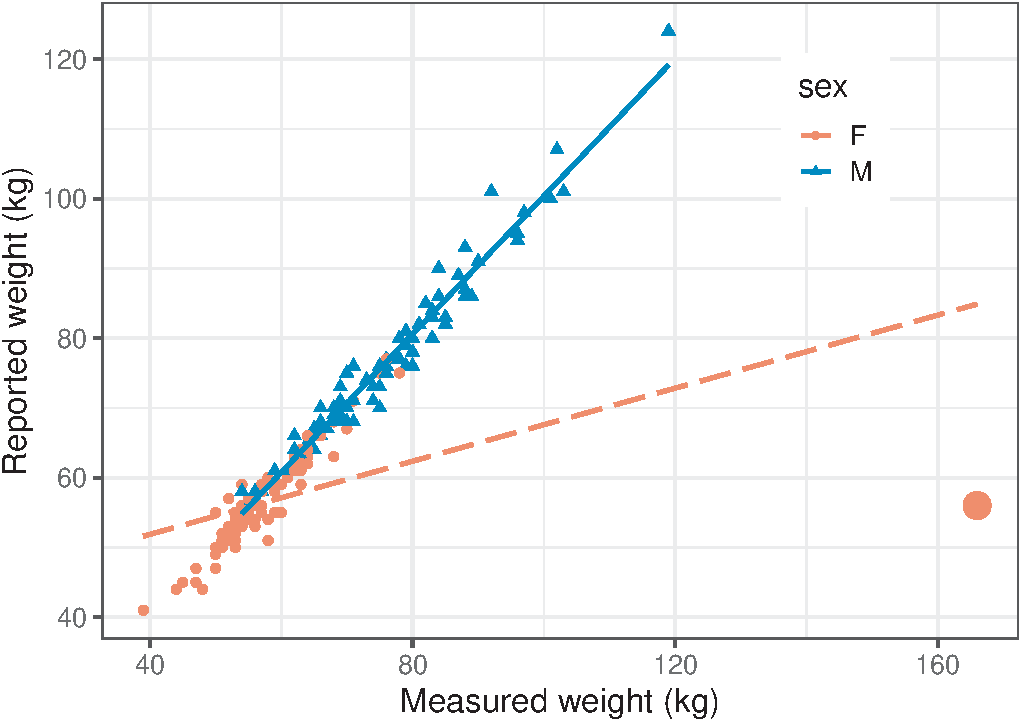
\includegraphics{figs/ch02/fig-ch02-davis-reg1-1.pdf}

}

\caption{\label{fig-ch02-davis-reg1}Regression for Davis' data on
reported weight and measures weight for men and women. Separate
regression lines, predicting reported weight from measured weight are
shown for males and females. One highly unusual point is highlighted.}

\end{figure}%

In this example, it was arguable that \(x\) and \(y\) axes should be
reversed, to determine how well measured weight can be predicted from
reported weight. In \texttt{ggplot} this can easily be done by reversing
the \texttt{x} and \texttt{y} aesthetics.

\begin{Shaded}
\begin{Highlighting}[]
\NormalTok{Davis }\SpecialCharTok{|\textgreater{}}
  \FunctionTok{ggplot}\NormalTok{(}\FunctionTok{aes}\NormalTok{(}\AttributeTok{y =}\NormalTok{ weight, }\AttributeTok{x =}\NormalTok{ repwt, }\AttributeTok{color =}\NormalTok{ sex, }\AttributeTok{shape=}\NormalTok{sex)) }\SpecialCharTok{+}
  \FunctionTok{geom\_point}\NormalTok{(}\AttributeTok{size =} \FunctionTok{ifelse}\NormalTok{(Davis}\SpecialCharTok{$}\NormalTok{weight}\SpecialCharTok{==}\DecValTok{166}\NormalTok{, }\DecValTok{6}\NormalTok{, }\DecValTok{2}\NormalTok{)) }\SpecialCharTok{+}
  \FunctionTok{labs}\NormalTok{(}\AttributeTok{y =} \StringTok{"Measured weight (kg)"}\NormalTok{, }\AttributeTok{x =} \StringTok{"Reported weight (kg)"}\NormalTok{) }\SpecialCharTok{+}
    \FunctionTok{geom\_smooth}\NormalTok{(}\AttributeTok{method =} \StringTok{"lm"}\NormalTok{, }\AttributeTok{formula =}\NormalTok{ y}\SpecialCharTok{\textasciitilde{}}\NormalTok{x, }\AttributeTok{se =} \ConstantTok{FALSE}\NormalTok{) }\SpecialCharTok{+}
  \FunctionTok{legend\_inside}\NormalTok{(}\FunctionTok{c}\NormalTok{(.}\DecValTok{8}\NormalTok{, .}\DecValTok{8}\NormalTok{))}
\end{Highlighting}
\end{Shaded}

\begin{figure}[H]

\centering{

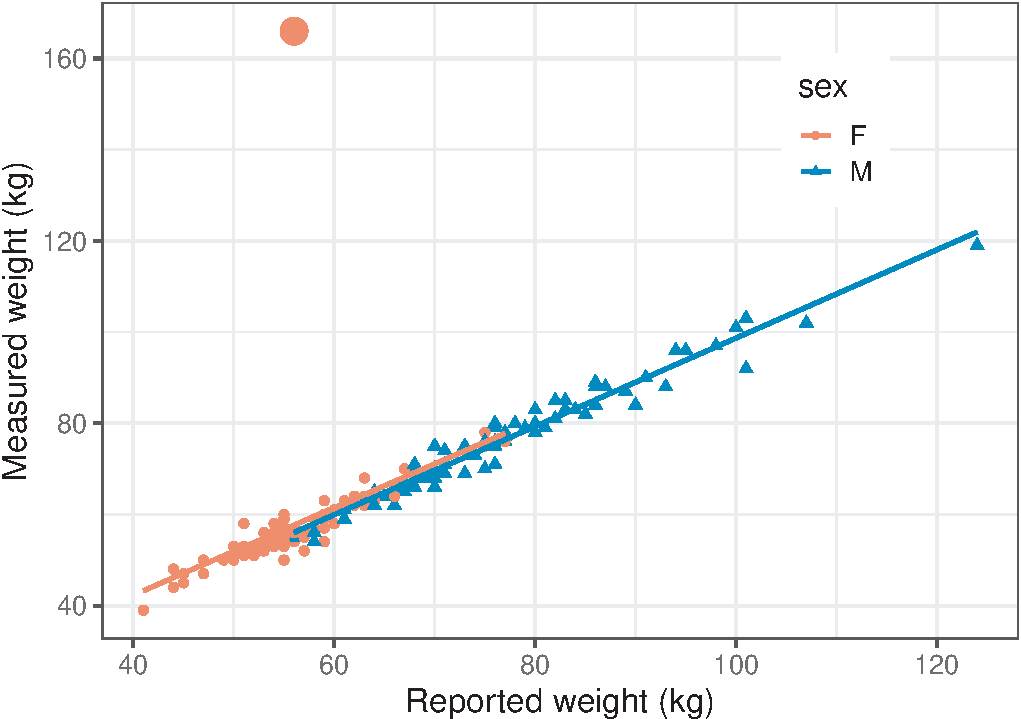
\includegraphics{figs/ch02/fig-ch02-davis-reg2-1.pdf}

}

\caption{\label{fig-ch02-davis-reg2}Regression for Davis' data on
reported weight and measures weight for men and women. Separate
regression lines, predicting measured weight from reported weight are
shown for males and females. The highly unusual point no longer has an
effect on the fitted lines.}

\end{figure}%

In Figure~\ref{fig-ch02-davis-reg2}, this discrepant observation again
stands out like a sore thumb, but it makes very little difference in the
fitted line for females. The reason is that this point is well within
the range of the \(x\) variable (\texttt{repwt}). To impact the slope of
the regression line, an observation must be unusual in\_both\_ \(x\) and
\(y\). We take up the topic of how to detect influential observations
and what to do about them in Chapter~\ref{sec-linear-models-plots}.

The value of such plots is not only that they can reveal possible
problems with an analysis, but also help identify their reasons and
suggest corrective action. What went wrong here? Examination of the
original data showed that this person switched the values, recording her
reported weight in the box for measured weight and vice versa.

\section{Plots for data analysis}\label{plots-for-data-analysis}

Visualization methods take an enormous variety of forms, but it is
useful to distinguish several broad categories according to their use in
data analysis:

\begin{itemize}
\item
  \textbf{data plots} : primarily plot the raw data, often with
  annotations to aid interpretation (regression lines and smooths, data
  ellipses, marginal distributions)
\item
  \textbf{reconnaissance plots} : with more than a few variables,
  reconnaissance plots provide a high-level, bird's-eye overview of the
  data, allowing you to see patterns that might not be visible in a set
  of separate plots. Some examples are scatterplot matrices, showing all
  bivariate plots of variables in a dataset; correlation diagrams, using
  visual glyphs to represent the correlations between all pairs of
  variables and ``trellis'' or faceted plots that show how a focal
  relation of one or more variables differs across values of other
  variables.
\item
  \textbf{model plots} : plot the results of a fitted model, such as a
  regression line or curve to show uncertainty, or a regression surface
  in 3D, or a plot of coefficients in model together with confidence
  intervals. Other model plots try to take into account that a fitted
  model may involve more variables than can be shown in a static 2D
  plot. Some examples of these are added variable plots, and marginal
  effect plots, both of which attempt to show the net relation of two
  focal variables, controlling or adjusting for other variables in a
  model.
\item
  \textbf{diagnostic plots} : indicating potential problems with the
  fitted model. These include residual plots, influence plots, plots for
  testing homogeneity of variance and so forth.
\item
  \textbf{dimension reduction plots} : plot representations of the data
  into a space of fewer dimensions than the number of variables in the
  dataset. Simple examples include principal components analysis (PCA)
  and the related biplots, and multidimensional scaling (MDS) methods.
\end{itemize}

We give some more details and a few examples in the sections that
follow.

\section{Data plots}\label{data-plots}

Data plots portray the data in a space where the coordinate axes are the
observed variables.

\begin{itemize}
\tightlist
\item
  1D plots include line plots, histograms and density estimates.
\item
  2D plots are most often scatterplots, but contour plots or hex-binned
  plots are also useful when the sample size is large.
\end{itemize}

\section{Model plots}\label{model-plots}

Model plots show the fitted or predicted values from a statistical model
and provide visual summaries\ldots{}

\section{Diagnostic plots}\label{diagnostic-plots}

\section{Principles of graphical
display}\label{principles-of-graphical-display}

{[}This could be a separate chapter{]}

\begin{itemize}
\tightlist
\item
  Criteria for assessing graphs: communication goals
\item
  Effective data display:

  \begin{itemize}
  \tightlist
  \item
    Make the data stand out
  \item
    Make graphical comparison easy
  \item
    Effect ordering: For variables and unordered factors, arrange them
    according to the effects to be seen
  \end{itemize}
\item
  Visual thinning: As the data becomes more complex, focus more on
  impactful summaries
\end{itemize}

\textbf{Package summary}

12 packages used here: broom, dplyr, forcats, ggplot2, knitr, lubridate,
purrr, readr, stringr, tibble, tidyr, tidyverse

\part{Exploratory Methods}

\chapter{Plots of Multivariate Data}\label{sec-multivariate_plots}

\begin{quote}
There is no excuse for failing to plot and look.

The greatest value of a picture is when it forces us to notice what we
never expected to see. --- John W. Tukey, \emph{Exploratory Data
Analysis}, 1977
\end{quote}

These quotes from John Tukey remind us that data analysis should nearly
always start with graphs to help us understand the main features of our
data. It is important to understand the general \emph{patterns} and
\emph{trends}: Are relationships increasing or decreasing? Are they
approximately linear or non-linear? But it is also important to spot
\emph{anomalies}: ``unusual'' observations, groups of points that seem
to differ from the rest, and so forth. As we saw with Anscombe's quartet
(Section~\ref{sec-anscombe}) numerical summaries hide features that are
immediately apparent in a plot.

This chapter introduces a toolbox of basic graphical methods for
visualizing multivariate datasets. It starts with some simple techniques
to enhance the basic scatterplot with graphical \emph{annotations} such
as fitted lines, curves and data ellipses to \emph{summarize} the
relation between two variables.

To visualize more than two variables, we can view all pairs of variables
in a scatterplot matrix or shift gears entirely to show multiple
variables along a set of parallel axes. As the number of variables
increases, we may need to suppress details with stronger summaries for a
high-level reconnaissance of our data terrain, as we do by zooming out
on a map. For example, we can simply remove the data points or make them
nearly transparent to focus on the visual summaries provided by fitted
lines or other graphical summaries.

\textbf{Packages}

In this chapter I use the following packages. Load them now:

\begin{Shaded}
\begin{Highlighting}[]
\FunctionTok{library}\NormalTok{(car)}
\FunctionTok{library}\NormalTok{(ggplot2)}
\FunctionTok{library}\NormalTok{(dplyr)}
\FunctionTok{library}\NormalTok{(tidyr)}
\FunctionTok{library}\NormalTok{(corrplot)}
\FunctionTok{library}\NormalTok{(corrgram)}
\FunctionTok{library}\NormalTok{(GGally)}
\FunctionTok{library}\NormalTok{(ggdensity)}
\FunctionTok{library}\NormalTok{(patchwork)}
\FunctionTok{library}\NormalTok{(ggpcp)}
\FunctionTok{library}\NormalTok{(tourr)}
\end{Highlighting}
\end{Shaded}

\section{Bivariate summaries}\label{sec-bivariate_summaries}

The basic scatterplot is the workhorse of multivariate data
visualization, showing how one variable, \(y\), often an outcome to be
explained by or varies with another, \(x\). It is a building block for
many useful techniques, so it is helpful to understand how it can be
used as a tool for thinking in a wider, multivariate context.

The essential idea is that we can start with a simple version of the
scatterplot and add annotations to show interesting features more
clearly. We consider the following here:

\begin{itemize}
\tightlist
\item
  \textbf{Smoothers}: Showing overall trends, perhaps in several forms,
  as visual summaries such as fitted regression lines or curves and
  nonparametric smoothers.
\item
  \textbf{Stratifiers}: Using color, shape or other features to identify
  subgroups; more generally, \emph{conditioning} on other variables in
  multi-panel displays;
\item
  \textbf{Data ellipses}: A compact 2D visual summary of bivariate
  linear relations and uncertainty assuming normality; more generally,
  contour plots of bivariate density.
\end{itemize}

\textbf{Example: Academic salaries}

Let's start with data on the academic salaries of faculty members
collected at a U.S. college for the purpose of assessing salary
differences between male and female faculty members, and perhaps address
anomalies in compensation. The dataset \texttt{carData::Salaries} gives
data on nine-month salaries and other variables for 397 faculty members
in the 2008-2009 academic year.

\begin{Shaded}
\begin{Highlighting}[]
\FunctionTok{data}\NormalTok{(Salaries, }\AttributeTok{package =} \StringTok{"carData"}\NormalTok{)}
\FunctionTok{str}\NormalTok{(Salaries)}
\CommentTok{\#\textgreater{} \textquotesingle{}data.frame\textquotesingle{}:    397 obs. of  6 variables:}
\CommentTok{\#\textgreater{}  $ rank         : Factor w/ 3 levels "AsstProf","AssocProf",..: 3 3 1 3 3 2 3 3 3 3 ...}
\CommentTok{\#\textgreater{}  $ discipline   : Factor w/ 2 levels "A","B": 2 2 2 2 2 2 2 2 2 2 ...}
\CommentTok{\#\textgreater{}  $ yrs.since.phd: int  19 20 4 45 40 6 30 45 21 18 ...}
\CommentTok{\#\textgreater{}  $ yrs.service  : int  18 16 3 39 41 6 23 45 20 18 ...}
\CommentTok{\#\textgreater{}  $ sex          : Factor w/ 2 levels "Female","Male": 2 2 2 2 2 2 2 2 2 1 ...}
\CommentTok{\#\textgreater{}  $ salary       : int  139750 173200 79750 115000 141500 97000 175000 147765 119250 129000 ...}
\end{Highlighting}
\end{Shaded}

The most obvious, but perhaps naive, predictor of \texttt{salary} is
\texttt{years.since.phd}. For simplicity, I'll refer to this as years of
``experience.'' Before looking at differences between males and females,
we would want consider faculty \texttt{rank} (related also to
\texttt{yrs.service}) and \texttt{discipline}, recorded here as
\texttt{"A"} (``theoretical'' departments) or \texttt{"B"} (``applied''
departments). But, for a basic plot, we will ignore these for now to
focus on what can be learned from plot annotations.

\begin{Shaded}
\begin{Highlighting}[]
\FunctionTok{library}\NormalTok{(ggplot2)}
\NormalTok{gg1 }\OtherTok{\textless{}{-}} \FunctionTok{ggplot}\NormalTok{(Salaries, }
       \FunctionTok{aes}\NormalTok{(}\AttributeTok{x =}\NormalTok{ yrs.since.phd, }\AttributeTok{y =}\NormalTok{ salary)) }\SpecialCharTok{+}
  \FunctionTok{geom\_jitter}\NormalTok{(}\AttributeTok{size =} \DecValTok{2}\NormalTok{) }\SpecialCharTok{+}
  \FunctionTok{scale\_y\_continuous}\NormalTok{(}\AttributeTok{labels =}\NormalTok{ scales}\SpecialCharTok{::}\FunctionTok{dollar\_format}\NormalTok{(}
    \AttributeTok{prefix=}\StringTok{"$"}\NormalTok{, }\AttributeTok{scale =} \FloatTok{0.001}\NormalTok{, }\AttributeTok{suffix =} \StringTok{"K"}\NormalTok{)) }\SpecialCharTok{+}
  \FunctionTok{labs}\NormalTok{(}\AttributeTok{x =} \StringTok{"Years since PhD"}\NormalTok{,}
       \AttributeTok{y =} \StringTok{"Salary"}\NormalTok{) }

\NormalTok{gg1 }\SpecialCharTok{+} \FunctionTok{geom\_rug}\NormalTok{(}\AttributeTok{position =} \StringTok{"jitter"}\NormalTok{, }\AttributeTok{alpha =} \DecValTok{1}\SpecialCharTok{/}\DecValTok{4}\NormalTok{)}
\end{Highlighting}
\end{Shaded}

\begin{figure}[H]

\centering{

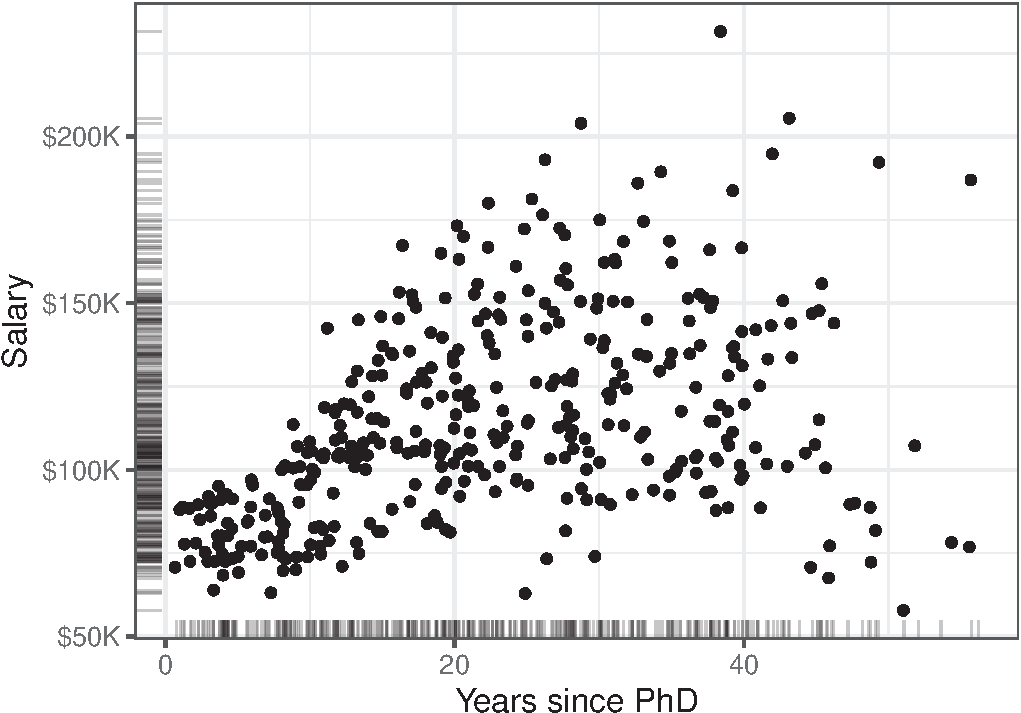
\includegraphics[width=0.9\textwidth,height=\textheight]{figs/ch03/fig-Salaries-scat-1.pdf}

}

\caption{\label{fig-Salaries-scat}Naive scatterplot of Salary vs.~years
since PhD, ignoring other variables, and without graphical annotations.}

\end{figure}%

There is quite a lot we can see ``just by looking'' at this simple plot,
but the main things are:

\begin{itemize}
\tightlist
\item
  Salary increases generally from 0 - 40 years since the PhD, but then
  maybe begins to drop off (partial retirement?);
\item
  Variability in salary increases among those with the same experience,
  a ``fan-shaped'' pattern that signals a violation of homogeneity of
  variance in simple regression;
\item
  Data beyond 50 years is thin, but there are some quite low salaries
  there. Adding rug plots to the X and Y axes is a simple but effective
  way to show the marginal distributions of the observations. Jitter and
  transparency helps to avoid overplotting due to discrete values.
\end{itemize}

\subsection{Smoothers}\label{smoothers}

Smoothers are among the most useful graphical annotations you can add to
such plots, giving a visual summary of how \(y\) changes with \(x\). The
most common smoother is a line showing the linear regression for \(y\)
given \(x\), expressed in math notation as
\(\mathbb{E} (y | x) = b_0 + b_1 x\). If there is doubt that a linear
relation is an adequate summary, you can try a quadratic or other
polynomial smoothers.

In \textbf{ggplot2}, these are easily added to a plot using
\texttt{geom\_smooth()} with \texttt{method\ =\ "lm"}, and a model
\texttt{formula}, which (by default) is \texttt{y\ \textasciitilde{}\ x}
for a linear relation or \texttt{y\ \textasciitilde{}\ poly(x,\ k)} for
a polynomial of degree \(k\).

\begin{Shaded}
\begin{Highlighting}[]
\NormalTok{gg1 }\SpecialCharTok{+} 
  \FunctionTok{geom\_smooth}\NormalTok{(}\AttributeTok{method =} \StringTok{"lm"}\NormalTok{, }\AttributeTok{formula =} \StringTok{"y \textasciitilde{} x"}\NormalTok{, }
              \AttributeTok{color =} \StringTok{"red"}\NormalTok{, }\AttributeTok{fill=} \StringTok{"pink"}\NormalTok{,}
              \AttributeTok{linewidth =} \DecValTok{2}\NormalTok{) }\SpecialCharTok{+}
  \FunctionTok{geom\_smooth}\NormalTok{(}\AttributeTok{method =} \StringTok{"lm"}\NormalTok{, }\AttributeTok{formula =} \StringTok{"y \textasciitilde{} poly(x,2)"}\NormalTok{, }
              \AttributeTok{color =} \StringTok{"darkgreen"}\NormalTok{, }\AttributeTok{fill =} \StringTok{"lightgreen"}\NormalTok{,}
              \AttributeTok{linewidth =} \DecValTok{2}\NormalTok{) }
\end{Highlighting}
\end{Shaded}

\begin{figure}[H]

\centering{

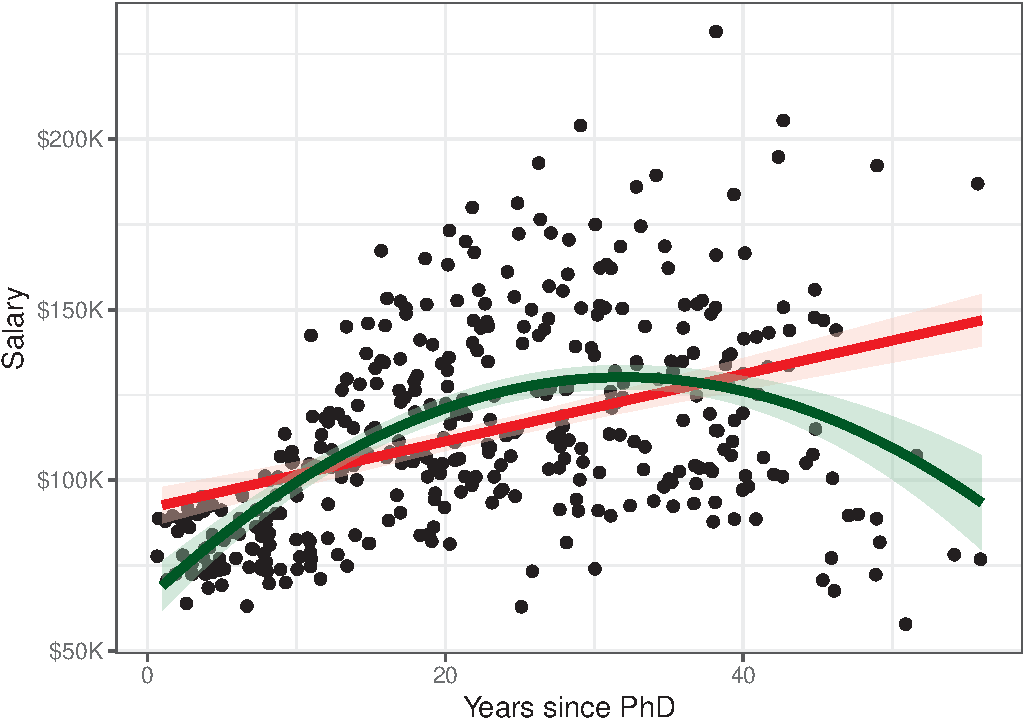
\includegraphics[width=0.8\textwidth,height=\textheight]{figs/ch03/fig-Salaries-lm-1.pdf}

}

\caption{\label{fig-Salaries-lm}Scatterplot of Salary vs.~years since
PhD, showing \textcolor{red}{linear} and
\textcolor{darkgreen}{quadratic} smooths with 95\% confidence bands.}

\end{figure}%

This serves to highlight some of our impressions from the basic
scatterplot shown in Figure~\ref{fig-Salaries-scat}, making them more
apparent. And that's precisely the point: the regression smoother draws
attention to a possible pattern that we can consider as a visual summary
of the data. You can think of this as showing what a linear (or
quadratic) regression ``sees'' in the data. Statistical tests can help
you decide if there is more evidence for a quadratic fit compared to the
simpler linear relation.

It is useful to also show some indication of \emph{uncertainty} (or
inversely, \emph{precision}) associated with the predicted values. Both
the linear and quadratic trends are shown in
Figure~\ref{fig-Salaries-lm} with 95\% pointwise confidence
bands.\footnote{Confidence bands allow us to visualize the uncertainty
  around a fitted regression curve, which can be of two types:
  \emph{pointwise intervals} or \emph{simultaneous intervals}. The
  default setting in `\texttt{ggplot2::geom\_smooth()} calculates
  pointwise intervals (using
  \texttt{stats::predict.lm(...,\ interval="confidence")} at a
  confidence level \(1-\alpha\) for the predicted response at \emph{each
  value} \(x_i\) of a predictor, and have the frequentist interpretation
  that over repeated sampling only \(100\;\alpha\) of the predictions at
  \(x_i\) will be outside that interval. In contrast, simultaneous
  intervals are calculated so that \(1 - \alpha\) is the probability
  that \emph{all of them} cover their corresponding true values
  simultaneously. These are necessarily wider than pointwise intervals.
  Commonly used methods for constructing simultaneous confidence bands
  in regression are the Bonferroni and Scheffé methods, which control
  the family-wise error rate over all values of \(x_i\). See
  \href{https://en.wikipedia.org/wiki/Confidence_and_prediction_bands}{}
  for precise definitions of these terms. These are different from a
  \emph{prediction band}, which is used to represent the uncertainty
  about the value of a \textbf{new} data-point on the curve, but subject
  to the additional variance reflected in one observation.} These are
necessarily narrower in the center of the range of \(x\) where there is
typically more data; they get wider toward the highest values of
experience where the data are thinner.

\subsubsection*{Non-parametric
smoothers}\label{non-parametric-smoothers}
\addcontentsline{toc}{subsubsection}{Non-parametric smoothers}

The most generally useful idea is a smoother that tracks an average
value, \(\mathbb{E} (y | x)\), of \(y\) as \(x\) varies across its'
range \emph{without} assuming any particular functional form, and so
avoiding the necessity to choose among
\texttt{y\ \textasciitilde{}\ poly(x,\ 1)}, or
\texttt{y\ \textasciitilde{}\ poly(x,\ 2)}, or
\texttt{y\ \textasciitilde{}\ poly(x,\ 3)}, etc.

Non-parametric smoothers attempt to estimate
\(\mathbb{E} (y | x) = f(x)\) where \(f(x)\) is some smooth function.
These typically use a collection of weighted \emph{local regressions}
for each \(x_i\) within a window centered at that value. In the method
called \emph{lowess} or \emph{loess}
(\citeproc{ref-Cleveland:79}{Cleveland, 1979};
\citeproc{ref-ClevelandDevlin:88}{Cleveland \& Devlin, 1988}), a weight
function is applied, giving greatest weight to \(x_i\) and a weight of 0
outside a window containing a certain fraction, \(s\), called
\emph{span}, of the nearest neighbors of \(x_i\). The fraction, \(s\),
is usually within the range \(1/3 \le s \le 2/3\), and it determines the
smoothness of the resulting curve; smaller values produce a wigglier
curve and larger values giving a smoother fit (an optimal span can be
determined by \(k\)-fold cross-validation to minimize a measure of
overall error of approximation).

Non-parametric regression is a broad topic; see Fox
(\citeproc{ref-Fox:2016:ARA}{2016}), Ch. 18 for a more general treatment
including smoothing splines, and Wood (\citeproc{ref-Wood:2006}{2006})
for generalized additive models, fit using \texttt{method\ =\ "gam"} in
\textbf{ggplot2}, which is the default when the largest group has more
than 1,000 observations.

Figure~\ref{fig-Salaries-loess} shows the addition of a loess smooth to
the plot in Figure~\ref{fig-Salaries-lm}, suppressing the confidence
band for the linear regression. The loess fit is nearly coincident with
the quadratic fit, but has a slightly wider confidence band.

\begin{Shaded}
\begin{Highlighting}[]
\NormalTok{gg1 }\SpecialCharTok{+} 
  \FunctionTok{geom\_smooth}\NormalTok{(}\AttributeTok{method =} \StringTok{"loess"}\NormalTok{, }\AttributeTok{formula =} \StringTok{"y \textasciitilde{} x"}\NormalTok{, }
              \AttributeTok{color =} \StringTok{"blue"}\NormalTok{, }\AttributeTok{fill =}\NormalTok{ scales}\SpecialCharTok{::}\FunctionTok{muted}\NormalTok{(}\StringTok{"blue"}\NormalTok{),}
              \AttributeTok{linewidth =} \DecValTok{2}\NormalTok{) }\SpecialCharTok{+}
  \FunctionTok{geom\_smooth}\NormalTok{(}\AttributeTok{method =} \StringTok{"lm"}\NormalTok{, }\AttributeTok{formula =} \StringTok{"y \textasciitilde{} x"}\NormalTok{, }\AttributeTok{se =} \ConstantTok{FALSE}\NormalTok{,}
              \AttributeTok{color =} \StringTok{"red"}\NormalTok{,}
              \AttributeTok{linewidth =} \DecValTok{2}\NormalTok{) }\SpecialCharTok{+}
  \FunctionTok{geom\_smooth}\NormalTok{(}\AttributeTok{method =} \StringTok{"lm"}\NormalTok{, }\AttributeTok{formula =} \StringTok{"y \textasciitilde{} poly(x,2)"}\NormalTok{, }
              \AttributeTok{color =} \StringTok{"darkgreen"}\NormalTok{, }\AttributeTok{fill =} \StringTok{"lightgreen"}\NormalTok{,}
              \AttributeTok{linewidth =} \DecValTok{2}\NormalTok{) }
\end{Highlighting}
\end{Shaded}

\begin{figure}[H]

\centering{

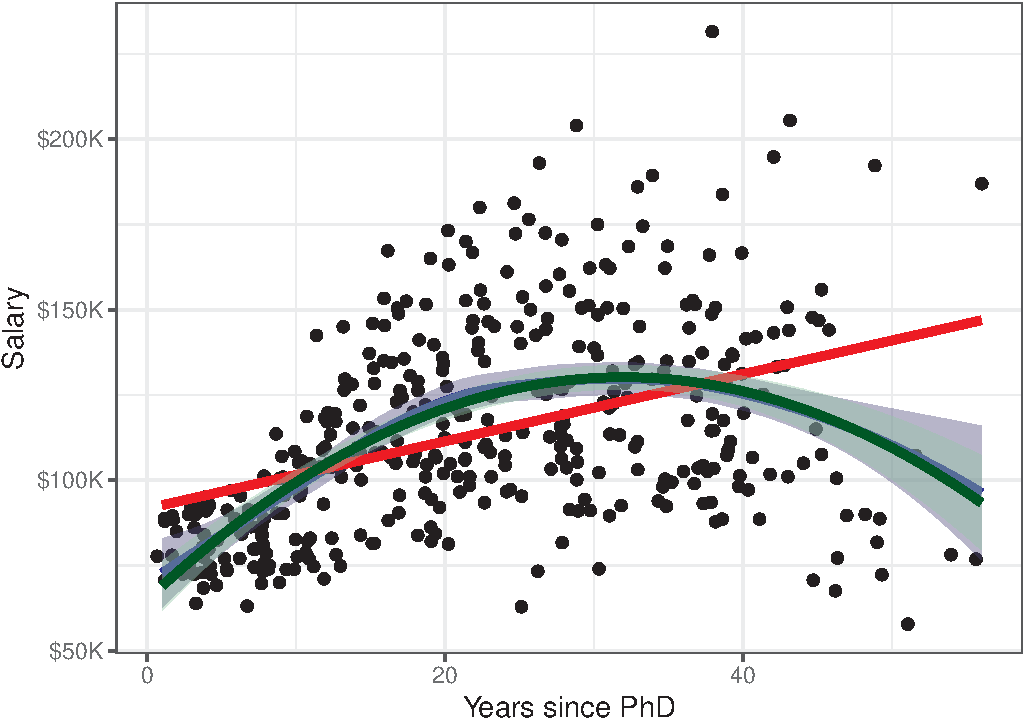
\includegraphics[width=0.8\textwidth,height=\textheight]{figs/ch03/fig-Salaries-loess-1.pdf}

}

\caption{\label{fig-Salaries-loess}Scatterplot of Salary vs.~years since
PhD, adding the loess smooth. The loess smooth curve and confidence band
in \textcolor{green}{green} is nearly indistinguishable from a quadratic
fit in \textcolor{blue}{blue}.}

\end{figure}%

But now comes an important question: is it reasonable that academic
salary should increase up to about 40 years since the PhD degree and
then decline? The predicted salary for someone still working 50 years
after earning their degree is about the same as a person at 15 years.
What else is going on here?

\subsection{Stratifiers}\label{stratifiers}

Very often, we have a main relationship of interest, but various groups
in the data are identified by discrete factors (like faculty
\texttt{rank} and \texttt{sex}, their type of \texttt{discipline} here),
or there are quantitative predictors for which the main relation might
vary. In the language of statistical models such effects are
\emph{interaction} terms, as in
\texttt{y\ \textasciitilde{}\ group\ +\ x\ +\ group:x}, where the term
\texttt{group:x} fits a different slope for each group and the grouping
variable is often called a \emph{moderator} variable. Common moderator
variables are ethnicity, health status, social class and level of
education. Moderators can also be continuous variables as in
\texttt{y\ \textasciitilde{}\ x1\ +\ x2\ +\ x1:x2}.

I call these \emph{stratifiers}, recognizing that we should consider
breaking down the overall relation to see whether and how it changes
over such ``other'' variables. Such variables are most often factors,
but we can cut a continuous variable into ranges (\emph{shingles}) and
do the same graphically. There are two general stratifying graphical
techniques:

\begin{itemize}
\item
  \textbf{Grouping}: Identify subgroups in the data by assigning
  different visual attributes, such as color, shape, line style, etc.
  within a single plot. This is quite natural for factors; quantitative
  predictors can be accommodated by cutting their range into ordered
  intervals. Grouping has the advantage that the levels of a grouping
  variable can be shown within the same plot, facilitating direct
  comparison.
\item
  \textbf{Conditioning}: Showing subgroups in different plot panels.
  This has the advantages that relations for the individual groups more
  easily discerned and one can easily stratify by two (or more) other
  variables jointly, but visual comparison is more difficult because the
  eye must scan from one panel to another.
\end{itemize}

\begin{tcolorbox}[enhanced jigsaw, breakable, left=2mm, bottomtitle=1mm, arc=.35mm, colframe=quarto-callout-note-color-frame, coltitle=black, title=\textcolor{quarto-callout-note-color}{\faInfo}\hspace{0.5em}{History Corner}, colback=white, toptitle=1mm, rightrule=.15mm, opacityback=0, colbacktitle=quarto-callout-note-color!10!white, titlerule=0mm, leftrule=.75mm, toprule=.15mm, bottomrule=.15mm, opacitybacktitle=0.6]

Recognition of the roles of visual grouping by factors within a panel
and conditioning in multi-panel displays was an important advance in the
development of modern statistical graphics. It began at A.T.\&T. Bell
Labs in Murray Hill, NJ in conjunction with the \textbf{S} language, the
mother of R.

Conditioning displays (originally called \emph{coplots}
(\citeproc{ref-ChambersHastie1991}{Chambers \& Hastie, 1991})) are
simply a collection of 1D, 2D or 3D plots separate panels for subsets of
the data broken down by one or more factors, or, for quantitative
variables, subdivided into a factor with several overlapping intervals
(\emph{shingles}). The first implementation was in \emph{Trellis} plots
(\citeproc{ref-Becker:1996:VDC}{Becker et al., 1996};
\citeproc{ref-Cleveland:85}{Cleveland, 1985}).

Trellis displays were extended in the \textbf{lattice} package
(\citeproc{ref-R-lattice}{Sarkar, 2024}), which offered:

\begin{itemize}
\tightlist
\item
  A \textbf{graphing syntax} similar to that used in statistical model
  formulas: \texttt{y\ \textasciitilde{}\ x\ \textbar{}\ g} conditions
  the data by the levels of \texttt{g}, with \texttt{\textbar{}} read as
  ``given''; two or more conditioning are specified as
  \texttt{y\ \textasciitilde{}\ x\ \textbar{}\ g1\ +\ g2\ +\ ...}, with
  \texttt{+} read as ``and''.
\item
  \textbf{Panel functions} define what is plotted in a given panel.
  \texttt{panel.xyplot()} is the default for scatterplots, plotting
  points, but you can add \texttt{panel.lmline()} for regression lines,
  \texttt{latticeExtra::panel.smoother()} for loess smooths and a wide
  variety of others.
\end{itemize}

The \textbf{car} package (\citeproc{ref-R-car}{Fox et al., 2023})
supports this graphing syntax in many of its functions. \textbf{ggplot2}
does not; it uses aesthetics (\texttt{aes()}), which map variables in
the data to visual characteristics in displays.

\end{tcolorbox}

The most obvious variable that affects academic salary is \texttt{rank},
because faculty typically get an increase in salary with a promotion
that carries through in their future salary. What can we see if we group
by \texttt{rank} and fit a separate smoothed curve for each?

In \texttt{ggplot2} thinking, grouping is accomplished simply by adding
an aesthetic, such as \texttt{color\ =\ rank}. What happens then is that
points, lines, smooths and other \texttt{geom\_*()} inherit the feature
that they are differentiated by color. In the case of
\texttt{geom\_smooth()}, we get a separate fit for each subset of the
data, according to \texttt{rank}.

\begin{Shaded}
\begin{Highlighting}[]
\CommentTok{\# make some re{-}useable pieces to avoid repetitions}
\NormalTok{scale\_salary }\OtherTok{\textless{}{-}}   \FunctionTok{scale\_y\_continuous}\NormalTok{(}
  \AttributeTok{labels =}\NormalTok{ scales}\SpecialCharTok{::}\FunctionTok{dollar\_format}\NormalTok{(}\AttributeTok{prefix=}\StringTok{"$"}\NormalTok{, }
                                 \AttributeTok{scale =} \FloatTok{0.001}\NormalTok{, }
                                 \AttributeTok{suffix =} \StringTok{"K"}\NormalTok{)) }
\CommentTok{\# position the legend inside the plot}
\NormalTok{legend\_pos }\OtherTok{\textless{}{-}} \FunctionTok{theme}\NormalTok{(}\AttributeTok{legend.position =} \StringTok{"inside"}\NormalTok{,}
                    \AttributeTok{legend.position.inside =} \FunctionTok{c}\NormalTok{(.}\DecValTok{1}\NormalTok{, }\FloatTok{0.95}\NormalTok{), }
                    \AttributeTok{legend.justification =} \FunctionTok{c}\NormalTok{(}\DecValTok{0}\NormalTok{, }\DecValTok{1}\NormalTok{))}

\FunctionTok{ggplot}\NormalTok{(Salaries, }
       \FunctionTok{aes}\NormalTok{(}\AttributeTok{x =}\NormalTok{ yrs.since.phd, }\AttributeTok{y =}\NormalTok{ salary, }
           \AttributeTok{color =}\NormalTok{ rank, }\AttributeTok{shape =}\NormalTok{ rank)) }\SpecialCharTok{+}
  \FunctionTok{geom\_point}\NormalTok{() }\SpecialCharTok{+}
\NormalTok{  scale\_salary }\SpecialCharTok{+}
  \FunctionTok{labs}\NormalTok{(}\AttributeTok{x =} \StringTok{"Years since PhD"}\NormalTok{,}
       \AttributeTok{y =} \StringTok{"Salary"}\NormalTok{) }\SpecialCharTok{+}
  \FunctionTok{geom\_smooth}\NormalTok{(}\FunctionTok{aes}\NormalTok{(}\AttributeTok{fill =}\NormalTok{ rank),}
                  \AttributeTok{method =} \StringTok{"loess"}\NormalTok{, }\AttributeTok{formula =} \StringTok{"y \textasciitilde{} x"}\NormalTok{, }
                  \AttributeTok{linewidth =} \DecValTok{2}\NormalTok{)  }\SpecialCharTok{+}
\NormalTok{  legend\_pos}
\end{Highlighting}
\end{Shaded}

\begin{figure}[H]

\centering{

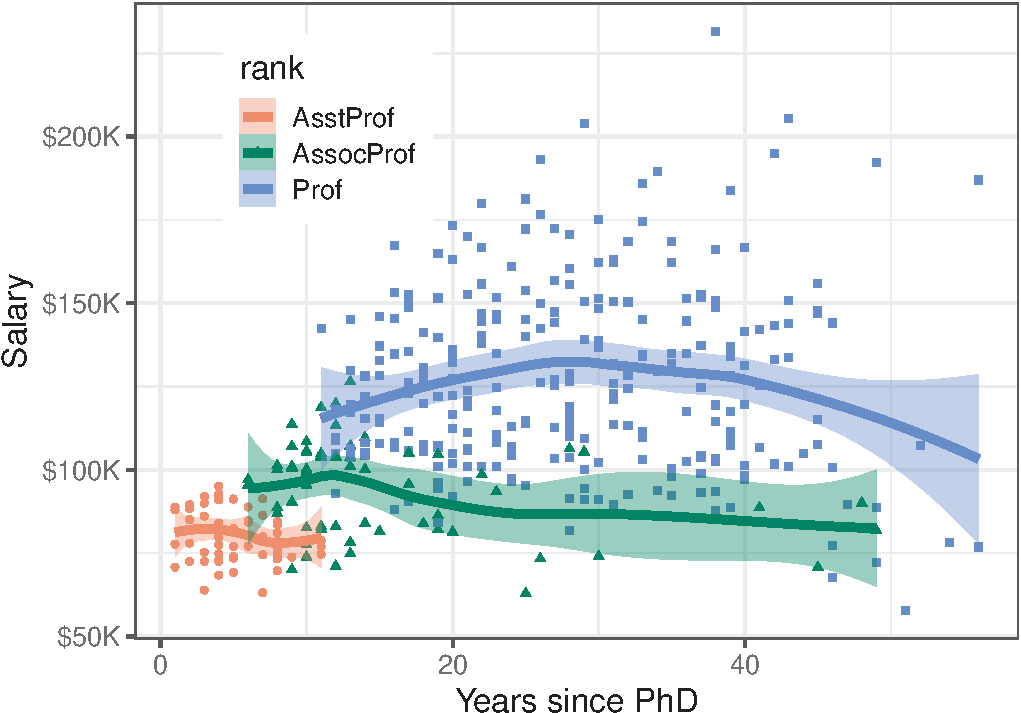
\includegraphics[width=0.8\textwidth,height=\textheight]{figs/ch03/fig-Salaries-rank-1.pdf}

}

\caption{\label{fig-Salaries-rank}Scatterplot of Salary vs.~years since
PhD, grouped by rank.}

\end{figure}%

Well, there is a different story here. Salaries generally occupy
separate vertical levels, increasing with academic rank. The horizontal
extents of the smoothed curves show their ranges. Within each rank there
is some initial increase after promotion, and then some tendency to
decline with increasing years. But, by and large, years since the PhD
doesn't make as much difference once we've taken academic rank into
account.

What about the \texttt{discipline} which is classified, perhaps
peculiarly, as ``theoretical'' vs.~``applied''? The values are just
\texttt{"A"} and \texttt{"B"}, so I map these to more meaningful labels
before making the plot.

\begin{Shaded}
\begin{Highlighting}[]
\NormalTok{Salaries }\OtherTok{\textless{}{-}}\NormalTok{ Salaries }\SpecialCharTok{|\textgreater{}}
  \FunctionTok{mutate}\NormalTok{(}\AttributeTok{discipline =} 
           \FunctionTok{factor}\NormalTok{(discipline, }
                  \AttributeTok{labels =} \FunctionTok{c}\NormalTok{(}\StringTok{"A: Theoretical"}\NormalTok{, }\StringTok{"B: Applied"}\NormalTok{)))}

\NormalTok{Salaries }\SpecialCharTok{|\textgreater{}}
  \FunctionTok{ggplot}\NormalTok{(}\FunctionTok{aes}\NormalTok{(}\AttributeTok{x =}\NormalTok{ yrs.since.phd, }\AttributeTok{y =}\NormalTok{ salary, }\AttributeTok{color =}\NormalTok{ discipline)) }\SpecialCharTok{+}
    \FunctionTok{geom\_point}\NormalTok{() }\SpecialCharTok{+}
\NormalTok{  scale\_salary }\SpecialCharTok{+}
  \FunctionTok{geom\_smooth}\NormalTok{(}\FunctionTok{aes}\NormalTok{(}\AttributeTok{fill =}\NormalTok{ discipline ),}
                \AttributeTok{method =} \StringTok{"loess"}\NormalTok{, }\AttributeTok{formula =} \StringTok{"y \textasciitilde{} x"}\NormalTok{, }
                \AttributeTok{linewidth =} \DecValTok{2}\NormalTok{) }\SpecialCharTok{+} 
  \FunctionTok{labs}\NormalTok{(}\AttributeTok{x =} \StringTok{"Years since PhD"}\NormalTok{,}
       \AttributeTok{y =} \StringTok{"Salary"}\NormalTok{) }\SpecialCharTok{+}
\NormalTok{  legend\_pos }
\end{Highlighting}
\end{Shaded}

\begin{figure}[H]

\centering{

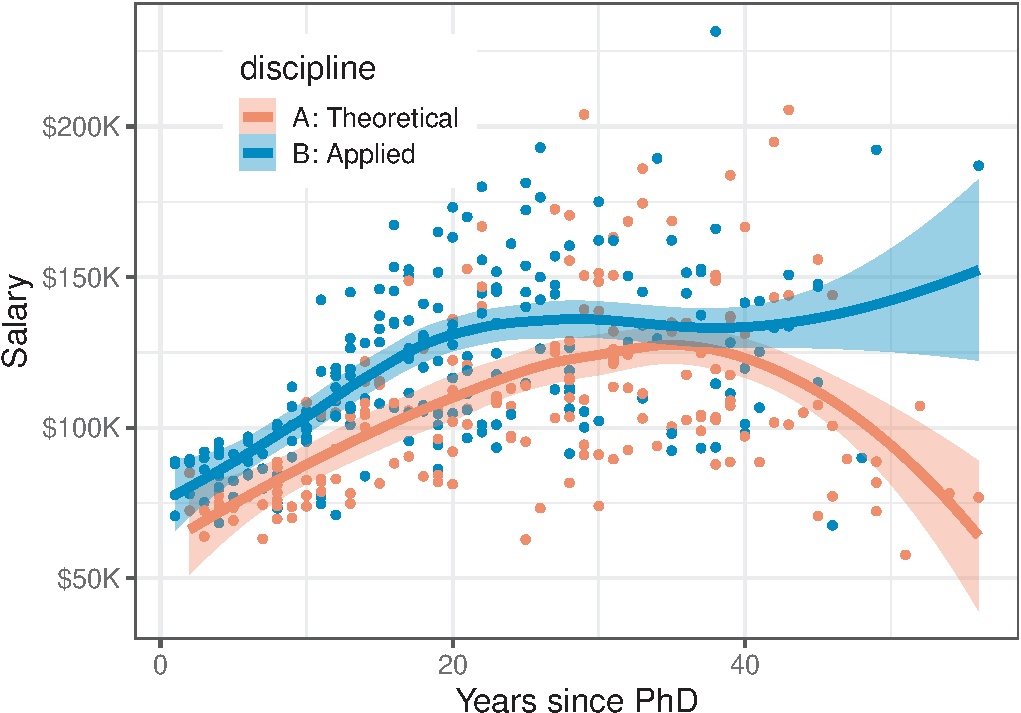
\includegraphics[width=0.8\textwidth,height=\textheight]{figs/ch03/fig-Salaries-discipline-1.pdf}

}

\caption{\label{fig-Salaries-discipline}Scatterplot of Salary vs.~years
since PhD, grouped by discipline.}

\end{figure}%

The story in Figure~\ref{fig-Salaries-discipline} is again different.
Faculty in applied disciplines on average earn about 10,000\$ more per
year on average than their theoretical colleagues.

\begin{Shaded}
\begin{Highlighting}[]
\NormalTok{Salaries }\SpecialCharTok{|\textgreater{}}
  \FunctionTok{group\_by}\NormalTok{(discipline) }\SpecialCharTok{|\textgreater{}}
  \FunctionTok{summarize}\NormalTok{(}\AttributeTok{mean =} \FunctionTok{mean}\NormalTok{(salary)) }
\CommentTok{\#\textgreater{} \# A tibble: 2 x 2}
\CommentTok{\#\textgreater{}   discipline        mean}
\CommentTok{\#\textgreater{}   \textless{}fct\textgreater{}            \textless{}dbl\textgreater{}}
\CommentTok{\#\textgreater{} 1 A: Theoretical 108548.}
\CommentTok{\#\textgreater{} 2 B: Applied     118029.}
\end{Highlighting}
\end{Shaded}

For both groups, there is an approximately linear relation up to about
30--40 years, but the smoothed curves then diverge into the region where
the data is thinner.

This result is more surprising than differences among faculty ranks. The
effect of annotation with smoothed curves as visual summaries is
apparent, and provides a stimulus to think about \emph{why} these
differences (if they are real) exist between theoretical and applied
professors, and maybe \emph{should} theoreticians be paid more!

\subsection{Conditioning}\label{conditioning}

The previous plots use grouping by color to plot the data for different
subsets inside the same plot window, making comparison among groups
easier, because they can be directly compared along a common vertical
scale \footnote{The classic study by Cleveland \& McGill
  (\citeproc{ref-ClevelandMcGill:84b}{1984});Cleveland \& McGill
  (\citeproc{ref-ClevelandMcGill:85}{1985}) shows that judgements of
  magnitude along a common scale are more accurate than those along
  separate, aligned scales.}. This gets messy, however, when there are
more than just a few levels, or worse---when there are two (or more)
variables for which we want to show separate effects. In such cases, we
can plot separate panels using the \texttt{ggplot2} concept of
\emph{faceting}. There are two options: \texttt{facet\_wrap()} takes one
or more conditioning variables and produces a ribbon of plots for each
combination of levels; \texttt{facet\_grid(row\ \textasciitilde{}\ col)}
takes two or more conditioning variables and arranges the plots in a 2D
array identified by the \texttt{row} and \texttt{col} variables.

Let's look at salary broken down by the combinations of discipline and
rank. Here, I chose to stratify using color by rank within each of
panels faceting by discipline. Because there is more going on in this
plot, a linear smooth is used to represent the trend.

\begin{Shaded}
\begin{Highlighting}[]
\NormalTok{Salaries }\SpecialCharTok{|\textgreater{}}
  \FunctionTok{ggplot}\NormalTok{(}\FunctionTok{aes}\NormalTok{(}\AttributeTok{x =}\NormalTok{ yrs.since.phd, }\AttributeTok{y =}\NormalTok{ salary, }
             \AttributeTok{color =}\NormalTok{ rank, }\AttributeTok{shape =}\NormalTok{ rank)) }\SpecialCharTok{+}
  \FunctionTok{geom\_point}\NormalTok{() }\SpecialCharTok{+}
\NormalTok{  scale\_salary }\SpecialCharTok{+}
  \FunctionTok{labs}\NormalTok{(}\AttributeTok{x =} \StringTok{"Years since PhD"}\NormalTok{,}
       \AttributeTok{y =} \StringTok{"Salary"}\NormalTok{) }\SpecialCharTok{+}
  \FunctionTok{geom\_smooth}\NormalTok{(}\FunctionTok{aes}\NormalTok{(}\AttributeTok{fill =}\NormalTok{ rank),}
              \AttributeTok{method =} \StringTok{"lm"}\NormalTok{, }\AttributeTok{formula =} \StringTok{"y \textasciitilde{} x"}\NormalTok{, }
              \AttributeTok{linewidth =} \DecValTok{2}\NormalTok{, }\AttributeTok{alpha =} \DecValTok{1}\SpecialCharTok{/}\DecValTok{4}\NormalTok{) }\SpecialCharTok{+}
  \FunctionTok{facet\_wrap}\NormalTok{(}\SpecialCharTok{\textasciitilde{}}\NormalTok{ discipline) }\SpecialCharTok{+}
\NormalTok{  legend\_pos}
\end{Highlighting}
\end{Shaded}

\begin{figure}[H]

\centering{

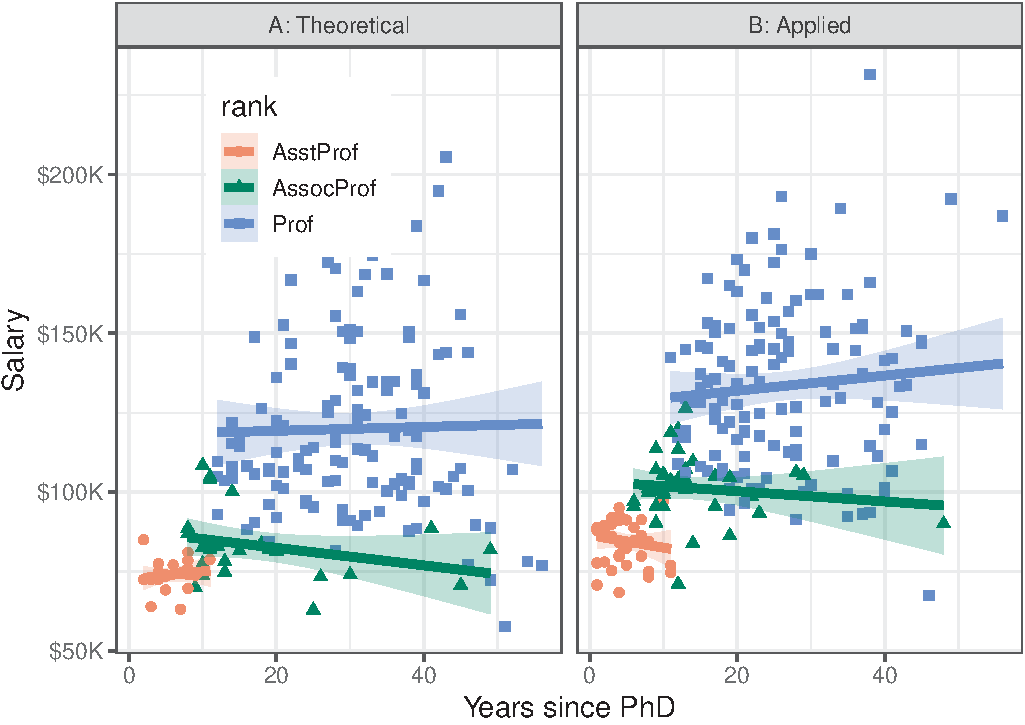
\includegraphics[width=1\textwidth,height=\textheight]{figs/ch03/fig-Salaries-faceted-1.pdf}

}

\caption{\label{fig-Salaries-faceted}Scatterplot of Salary vs.~years
since PhD, grouped by rank, with separate panels for discipline.}

\end{figure}%

Once both of these factors are taken into account, there does not seem
to be much impact of years of service. Salaries in theoretical
disciplines are noticeably greater than those in applied disciplines at
all ranks, and there are even greater differences among ranks.

Finally, to shed light on the question that motivated this example---
are there anomalous differences in salary for men and women--- we can
look at differences in salary according to sex, when discipline and rank
are taken into account. To do this graphically, condition by both
variables, but use
\texttt{facet\_grid(discipline\ \textasciitilde{}\ rank)} to arrange
their combinations in a grid whose rows are the levels of
\texttt{discipline} and columns are those of \texttt{rank}. I want to
make the comparison of males and females most direct, so I use
\texttt{color\ =\ sex} to stratify the panels. The smoothed regression
lines and error bands are calculated separately for each combination of
discipline, rank and sex.

\begin{Shaded}
\begin{Highlighting}[]
\NormalTok{Salaries }\SpecialCharTok{|\textgreater{}}
  \FunctionTok{ggplot}\NormalTok{(}\FunctionTok{aes}\NormalTok{(}\AttributeTok{x =}\NormalTok{ yrs.since.phd, }\AttributeTok{y =}\NormalTok{ salary, }\AttributeTok{color =}\NormalTok{ sex)) }\SpecialCharTok{+}
  \FunctionTok{geom\_point}\NormalTok{() }\SpecialCharTok{+}
\NormalTok{  scale\_salary }\SpecialCharTok{+}
  \FunctionTok{labs}\NormalTok{(}\AttributeTok{x =} \StringTok{"Years since PhD"}\NormalTok{,}
       \AttributeTok{y =} \StringTok{"Salary"}\NormalTok{) }\SpecialCharTok{+}
  \FunctionTok{geom\_smooth}\NormalTok{(}\FunctionTok{aes}\NormalTok{(}\AttributeTok{fill =}\NormalTok{ sex),}
              \AttributeTok{method =} \StringTok{"lm"}\NormalTok{, }\AttributeTok{formula =} \StringTok{"y \textasciitilde{} x"}\NormalTok{,}
              \AttributeTok{linewidth =} \DecValTok{2}\NormalTok{, }\AttributeTok{alpha =} \DecValTok{1}\SpecialCharTok{/}\DecValTok{4}\NormalTok{) }\SpecialCharTok{+}
  \FunctionTok{facet\_grid}\NormalTok{(discipline }\SpecialCharTok{\textasciitilde{}}\NormalTok{ rank) }\SpecialCharTok{+}
  \FunctionTok{theme\_bw}\NormalTok{(}\AttributeTok{base\_size =} \DecValTok{14}\NormalTok{) }\SpecialCharTok{+} 
\NormalTok{  legend\_pos}
\end{Highlighting}
\end{Shaded}

\begin{figure}[H]

\centering{

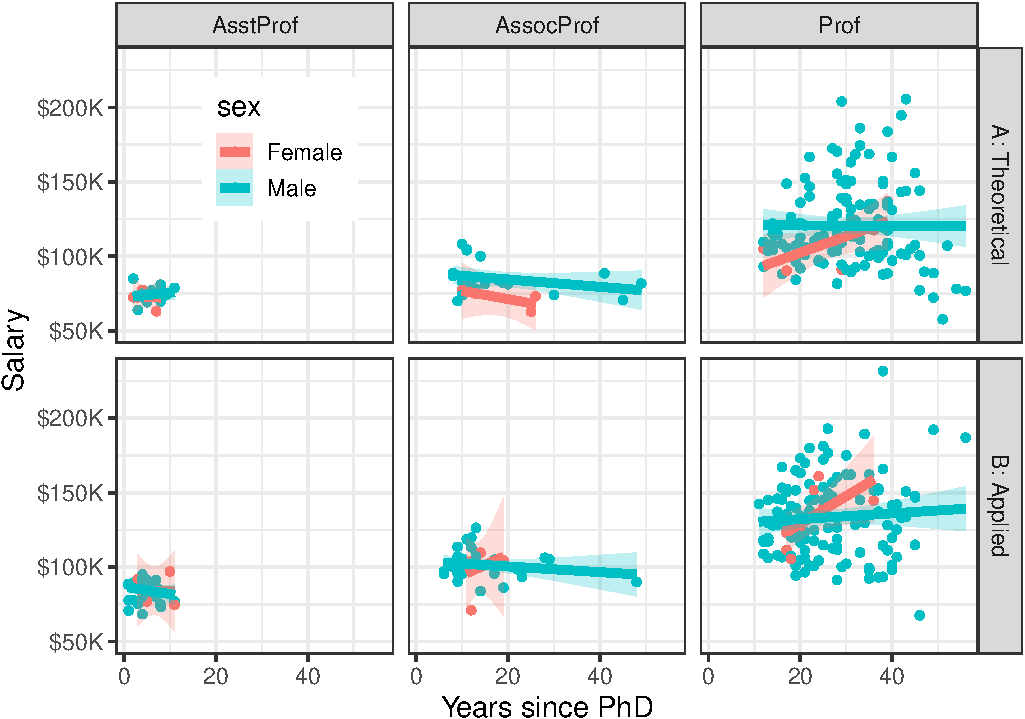
\includegraphics[width=1\textwidth,height=\textheight]{figs/ch03/fig-Salaries-facet-sex-1.pdf}

}

\caption{\label{fig-Salaries-facet-sex}Scatterplot of Salary vs.~years
since PhD, grouped by sex, faceted by discipline and rank.}

\end{figure}%

\section{Data Ellipses}\label{sec-data-ellipse}

The \emph{data ellipse} (\citeproc{ref-Monette:90}{Monette, 1990}), or
\emph{concentration ellipse} (\citeproc{ref-Dempster:69}{Dempster,
1969}) is a remarkably simple and effective display for viewing and
understanding bivariate relationships in multivariate data. The data
ellipse is typically used to add a visual summary to a scatterplot, that
shows all together the means, standard deviations, correlation, and
slope of the regression line for two variables, perhaps stratified by
another variable. Under the classical assumption that the data are
bivariate normally distributed, the data ellipse is also a
\textbf{sufficient} visual summary, in the sense that it captures
\textbf{all} relevant features of the data. See Friendly et al.
(\citeproc{ref-Friendly-etal:ellipses:2013}{2013}) for a complete
discussion of the role of ellipsoids in statistical data visualization.

It is based on the idea that in a bivariate normal distribution, the
contours of equal probability form a series of concentric ellipses. If
the variables were uncorrelated and had the same variances, these would
be circles, and Euclidean distance would measure the distance of each
observation from the mean. When the variables are correlated, a
different measure, \emph{Mahalanobis distance} is the proper measure of
how far a point is from the mean, taking the correlation into account.

\begin{figure}

\centering{

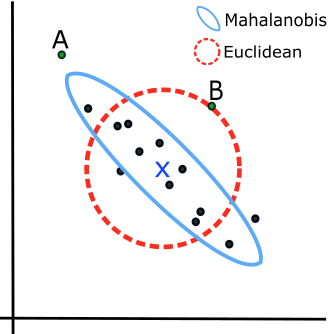
\includegraphics[width=0.6\textwidth,height=\textheight]{images/mahalanobis.png}

}

\caption{\label{fig-mahalanobis}2D data with curves of constant distance
from the centroid. The blue solid ellipse shows a contour of constant
Mahalanobis distance, taking the correlation into account; the dashed
red circle is a contour of equal Euclidean distance. Given the data
points, Which of the points \textbf{A} and \textbf{B} is further from
the mean (X)? \emph{Source}: Re-drawn from
\href{https://ouzhang.rbind.io/2020/11/16/outliers-part4/}{Ou Zhang}}

\end{figure}%

To illustrate, Figure~\ref{fig-mahalanobis} shows a scatterplot with
labels for two points, ``A'' and ``B''. Which is further from the mean,
``X''? A contour of constant Euclidean distance, shown by the
\textcolor{red}{red} dashed circle, ignores the apparent negative
correlation, so point ``A'' is further. The \textcolor{blue}{blue}
ellipse for Mahalanobis distance takes the correlation into account, so
point ``B'' has a greater distance from the mean.

Mathematically, Euclidean (squared) distance for \(p\) variables,
\(j = 1, 2, \dots , p\), is just a generalization of the square of a
univariate standardized (\(z\)) score, \(z^2 = [(y - \bar{y}) / s]^2\),

\[
D_E^2 (\mathbf{y}) = \sum_j^p z_j^2 = \mathbf{z}^\textsf{T}  \mathbf{z} = (\mathbf{y} - \bar{\mathbf{y}})^\textsf{T} \operatorname{diag}(\mathbf{S})^{-1} (\mathbf{y} - \bar{\mathbf{y}}) \; ,
\] where \(\mathbf{S}\) is the sample variance-covariance matrix,
\(\mathbf{S} = ({n-1})^{-1} \sum_{i=1}^n (\mathbf{y}_i - \bar{\mathbf{y}})^\textsf{T} (\mathbf{y}_i - \bar{\mathbf{y}})\).

Mahalanobis' distance takes the correlations into account simply by
using the covariances as well as the variances,
\begin{equation}\phantomsection\label{eq-Dsq}{
D_M^2 (\mathbf{y}) = (\mathbf{y} - \bar{\mathbf{y}})^\mathsf{T} S^{-1} (\mathbf{y} - \bar{\mathbf{y}}) \; .
}\end{equation}

In Equation~\ref{eq-Dsq}, the inverse \(S^{-1}\) serves to ``divide''
the matrix
\((\mathbf{y} - \bar{\mathbf{y}})^\mathsf{T} (\mathbf{y} - \bar{\mathbf{y}})\)
of squared distances by the variances (and covariances) of the
variables, as in the univariate case.

For \(p\) variables, the data \emph{ellipsoid} \(\mathcal{E}_c\) of size
\(c\) is a \(p\)-dimensional ellipse, defined as the set of points
\(\mathbf{y} = (y_1, y_2, \dots y_p)\) whose squared Mahalanobis
distance, \(D_M^2 ( \mathbf{y} )\) is less than or equal to \(c^2\), \[
\mathcal{E}_c (\bar{\mathbf{y}}, \mathbf{S}) := \{ D_M^2 (\mathbf{y}) \le c^2 \} \; .
\] A computational definition recognizes that the boundary of the
ellipsoid can be found by transforming a unit sphere centered at the
origin,
\(\text{radius}(\mathcal{P}) : \{ \mathbf{x}^\textsf{T} \mathbf{x}= 1\}\),
by \(\mathbf{S}^{1/2}\) and then shifting that to centroid of the data,

\[
\mathcal{E}_c (\bar{\mathbf{y}}, \mathbf{S}) = \bar{\mathbf{y}} \; \oplus \; \mathbf{S}^{1/2} \, \mathcal{P} 
\] where \(\mathbf{S}^{1/2}\) represents a rotation and scaling and
\(\oplus\) represents translation to a new centroid. The matrix
\(\mathbf{S}^{1/2}\) is commonly computed as the Choleski factor of
\(\mathbf{S}\). Slightly abusing notation and taking the unit sphere as
given (like an identity matrix), we can write the data ellipsoid as
simply

\[
\mathcal{E}_c (\bar{\mathbf{y}}, \mathbf{S}) = \bar{\mathbf{y}} \; \oplus \; \sqrt{\mathbf{S}} \:\: .
\]

When \(\mathbf{y}\) is (at least approximately) bivariate normal,
\(D_M^2(\mathbf{y})\) has a large-sample \(\chi^2_2\) distribution
(\(\chi^2\) with 2 df), so taking \(c^2 = \chi^2_2 (0.68) = 2.28\) gives
a ``1 standard deviation bivariate ellipse,'' an analog of the standard
interval \(\bar{y} \pm 1 s\), while
\(c^2 = \chi^2_2 (0.95) = 5.99 \approx 6\) gives a data ellipse of 95\%
coverage.

\subsection{Ellipse properties}\label{ellipse-properties}

The essential ideas of correlation and regression and their relation to
ellipses go back to Galton (\citeproc{ref-Galton:1886}{1886}). Galton's
goal was to predict (or explain) how a heritable trait, \(Y\), (e.g.,
height) of children was related to that of their parents, \(X\). He made
a semi-graphic table of the frequencies of 928 observations of the
average height of father and mother versus the height of their child,
shown in Figure~\ref{fig-galton-corr}. He then drew smoothed contour
lines of equal frequencies and had the wonderful visual insight that
these formed concentric shapes that were tolerably close to ellipses.

He then calculated summaries, \(\text{Ave}(Y | X)\), and, for symmetry,
\(\text{Ave}(X | Y)\), and plotted these as lines of means on his
diagram. Lo and behold, he had a second visual insight: the lines of
means of (\(Y | X\)) and (\(X | Y\)) corresponded approximately to the
loci of horizontal and vertical tangents to the concentric ellipses. To
complete the picture, he added lines showing the major and minor axes of
the family of ellipses (which turned out to be the principal components)
with the result shown in Figure~\ref{fig-galton-corr}.

\begin{figure}

\centering{

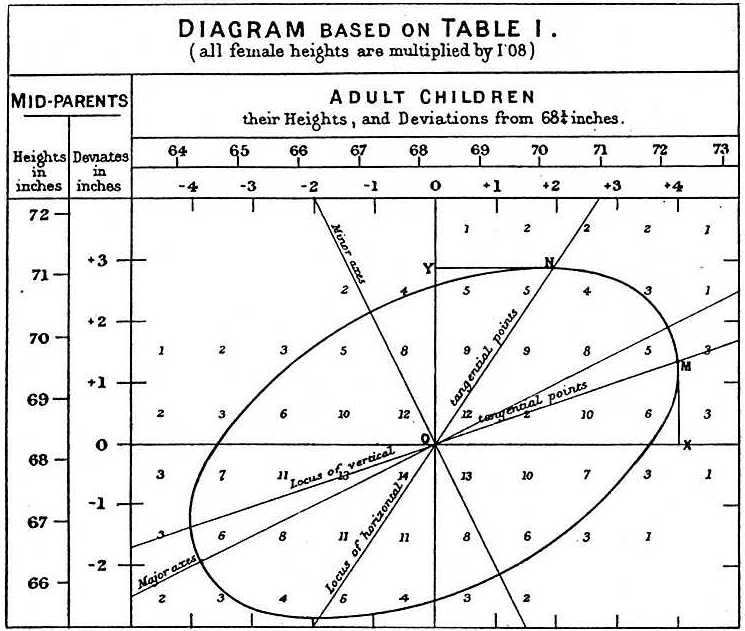
\includegraphics[width=0.7\textwidth,height=\textheight]{images/galton-corr.jpg}

}

\caption{\label{fig-galton-corr}Galton's 1886 diagram, showing the
relationship of height of children to the average of their parents'
height. The diagram is essentially an overlay of a geometrical
interpretation on a bivariate grouped frequency distribution, shown as
numbers.}

\end{figure}%

For two variables, \(x\) and \(y\), the remarkable properties of the
data ellipse are illustrated in Figure~\ref{fig-galton-ellipse-r}, a
modern reconstruction of Galton's diagram.

\begin{figure}

\centering{

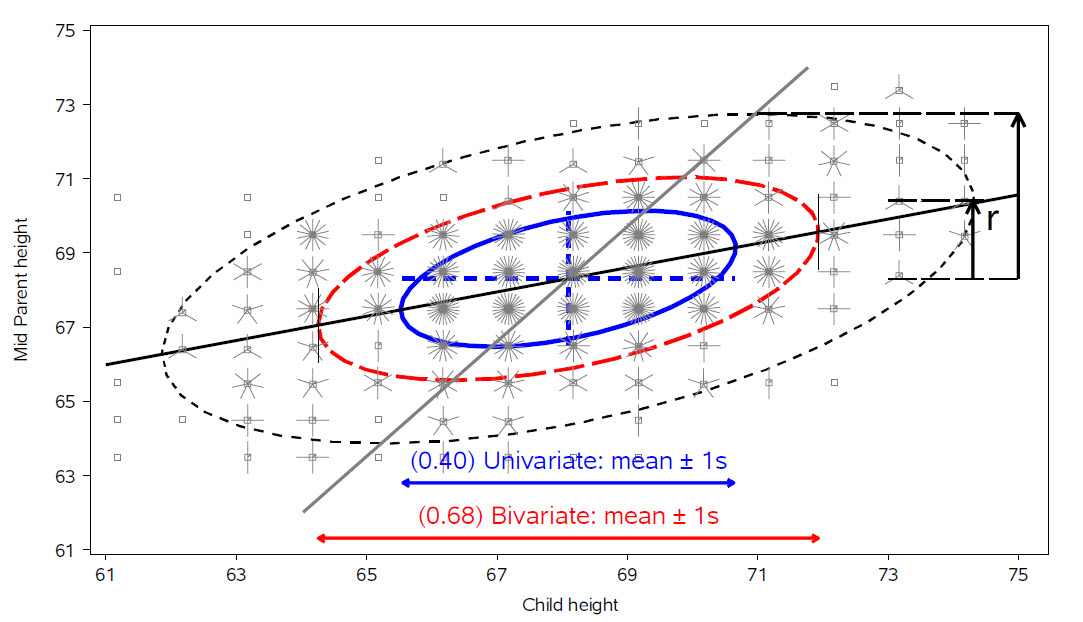
\includegraphics[width=1\textwidth,height=\textheight]{images/galton-ellipse-r.jpg}

}

\caption{\label{fig-galton-ellipse-r}Sunflower plot of Galton's data on
heights of parents and their children (in.), with 40\%, 68\% and 95\%
data ellipses and the regression lines of \(y\) on \(x\) (black) and
\(x\) on \(y\) (grey).}

\end{figure}%

\begin{itemize}
\item
  The ellipses have the mean vector \((\bar{x}, \bar{y})\) as their
  center.
\item
  The lengths of arms of the \textcolor{blue}{blue} dashed central cross
  show the standard deviations of the variables, which correspond to the
  shadows of the ellipse covering 40\% of the data. These are the
  bivariate analogs of the standard intervals \(\bar{x} \pm 1 s_x\) and
  \(\bar{y} \pm 1 s_y\).
\item
  More generally, shadows (projections) on the coordinate axes, or any
  linear combination of them, give any standard interval,
  \(\bar{x} \pm k s_x\) and \(\bar{y} \pm k s_y\). Those with
  \(k=1, 1.5, 2.45\), have bivariate coverage 40\%, 68\% and 95\%
  respectively, corresponding to these quantiles of the \(\chi^2\)
  distribution with 2 degrees of freedom, i.e.,
  \(\chi^2_2 (.40) \approx 1^2\), \(\chi^2_2 (.68) \approx 1.5^2\), and
  \(\chi^2_2 (.95) \approx 2.45\). The shadows of the 68\% ellipse are
  the bivariate analog of a univariate \(\bar{x} \pm 1 s_x\) interval.
\item
  The regression line predicting \(y\) from \(x\) goes through the
  points where the ellipses have vertical tangents. The \emph{other}
  regression line, predicting \(x\) from \(y\) goes through the points
  of horizontal tangency.
\item
  The correlation \(r(x, y)\) is the ratio of the vertical segment from
  the mean of \(y\) to the regression line to the vertical segment going
  to the top of the ellipse as shown at the right of the figure. It is
  \(r = 0.46\) in this example.
\item
  The residual standard deviation,
  \(s_e = \sqrt{MSE} = \sqrt{\Sigma (y - \bar{y})^2 / n-2}\), is the
  half-length of the ellipse at the mean \(\bar{x}\).
\end{itemize}

Because Galton's values of \texttt{parent} and \texttt{child} height
were recorded in class intervals of 1 in., they are shown as sunflower
symbols in Figure~\ref{fig-galton-ellipse-r}, with multiple `petals'
reflecting the number of observations at each location. This plot
(except for annotations) is constructed using \texttt{sunflowerplot()}
and \texttt{car::dataEllipse()} for the ellipses.

\begin{Shaded}
\begin{Highlighting}[]
\FunctionTok{data}\NormalTok{(Galton, }\AttributeTok{package =} \StringTok{"HistData"}\NormalTok{)}

\FunctionTok{sunflowerplot}\NormalTok{(parent }\SpecialCharTok{\textasciitilde{}}\NormalTok{ child, }\AttributeTok{data=}\NormalTok{Galton, }
      \AttributeTok{xlim=}\FunctionTok{c}\NormalTok{(}\DecValTok{61}\NormalTok{,}\DecValTok{75}\NormalTok{), }
      \AttributeTok{ylim=}\FunctionTok{c}\NormalTok{(}\DecValTok{61}\NormalTok{,}\DecValTok{75}\NormalTok{), }
      \AttributeTok{seg.col=}\StringTok{"black"}\NormalTok{, }
        \AttributeTok{xlab=}\StringTok{"Child height"}\NormalTok{, }
      \AttributeTok{ylab=}\StringTok{"Mid Parent height"}\NormalTok{)}

\NormalTok{y.x }\OtherTok{\textless{}{-}} \FunctionTok{lm}\NormalTok{(parent }\SpecialCharTok{\textasciitilde{}}\NormalTok{ child, }\AttributeTok{data=}\NormalTok{Galton)     }\CommentTok{\# regression of y on x}
\FunctionTok{abline}\NormalTok{(y.x, }\AttributeTok{lwd=}\DecValTok{2}\NormalTok{)}
\NormalTok{x.y }\OtherTok{\textless{}{-}} \FunctionTok{lm}\NormalTok{(child }\SpecialCharTok{\textasciitilde{}}\NormalTok{ parent, }\AttributeTok{data=}\NormalTok{Galton)     }\CommentTok{\# regression of x on y}
\NormalTok{cc }\OtherTok{\textless{}{-}} \FunctionTok{coef}\NormalTok{(x.y)}
\FunctionTok{abline}\NormalTok{(}\SpecialCharTok{{-}}\NormalTok{cc[}\DecValTok{1}\NormalTok{]}\SpecialCharTok{/}\NormalTok{cc[}\DecValTok{2}\NormalTok{], }\DecValTok{1}\SpecialCharTok{/}\NormalTok{cc[}\DecValTok{2}\NormalTok{], }\AttributeTok{lwd=}\DecValTok{2}\NormalTok{, }\AttributeTok{col=}\StringTok{"gray"}\NormalTok{)}

\FunctionTok{with}\NormalTok{(Galton, }
\NormalTok{     car}\SpecialCharTok{::}\FunctionTok{dataEllipse}\NormalTok{(child, parent, }
         \AttributeTok{plot.points=}\ConstantTok{FALSE}\NormalTok{, }
         \AttributeTok{levels=}\FunctionTok{c}\NormalTok{(}\FloatTok{0.40}\NormalTok{, }\FloatTok{0.68}\NormalTok{, }\FloatTok{0.95}\NormalTok{), }
         \AttributeTok{lty=}\DecValTok{1}\SpecialCharTok{:}\DecValTok{3}\NormalTok{)}
\NormalTok{    )}
\end{Highlighting}
\end{Shaded}

Finally, as Galton noted in his diagram, the principal major and minor
axes of the ellipse have important statistical properties. Pearson
(\citeproc{ref-Pearson:1901}{1901}) would later show that their
directions are determined by the eigenvectors
\(\mathbf{v}_1, \mathbf{v}_2, \dots\) of the covariance matrix
\(\mathbf{S}\) and their radii by the square roots,
\(\sqrt{\mathbf{v}_1}, \sqrt{\mathbf{v}_1}, \dots\) of the corresponding
eigenvalues.

\subsection{R functions for data
ellipses}\label{r-functions-for-data-ellipses}

A number of packages provide functions for drawing data ellipses in a
scatterplot, with various features.

\begin{itemize}
\tightlist
\item
  \texttt{car::scatterplot()}: uses base R graphics to draw 2D
  scatterplots, with a wide variety of plot enhancements including
  linear and non-parametric smoothers (loess, gam), a formula method,
  e.g., \texttt{y\ \textasciitilde{}\ x\ \textbar{}\ group}, and marking
  points and lines using symbol shape, color, etc. Importantly, the
  \textbf{car} package generally allows automatic identification of
  ``noteworthy'' points by their labels in the plot using a variety of
  methods. For example, \texttt{method\ =\ "mahal"} labels cases with
  the most extreme Mahalanobis distances; \texttt{method\ =\ "r"}
  selects points according to their value of \texttt{abs(y)}, which is
  appropriate in residual plots.
\item
  \texttt{car::dataEllipse()}: plots classical or robust data (using
  \texttt{MASS::cov/trob()}) ellipses for one or more groups, with the
  same facilities for point identification.
\item
  \texttt{heplots::covEllipses()}: draws classical or robust data
  ellipses for one or more groups in a one-way design and optionally for
  the pooled total sample, where the focus is on homogeneity of
  within-group covariance matrices.
\item
  \texttt{ggplot2::stat\_ellipse()}: uses the calculation methods of
  \texttt{car::dataEllipse()} to add unfilled (\texttt{geom\ =\ "path"})
  or filled (\texttt{geom\ =\ polygon"}) data ellipses in a
  \texttt{ggplot} scatterplot, using inherited aesthetics.
\end{itemize}

\subsection{Example: Canadian occupational prestige}\label{sec-prestige}

These examples use the data on the prestige of 102 occupational
categories and other measures from the 1971 Canadian Census, recorded in
\texttt{carData::Prestige}.\footnote{The dataset was collected by
  Bernard Blishen, William Carroll and Catherine Moore, but apparently
  unpublished. A version updated to the 1981 census is described in
  Blishen et al. (\citeproc{ref-Blishen-etal-1987}{1987}).} Our interest
is in understanding how \texttt{prestige} (the Pineo \& Porter
(\citeproc{ref-PineoPorter2008}{2008}) prestige score for an
occupational category, derived from a social survey) is related to
census measures of the average education, income, percent women of
incumbents in those occupations. Occupation \texttt{type} is a factor
with levels \texttt{"bc"} (blue collar), \texttt{"wc"} (white collar)
and \texttt{"prof"} (professional).

\begin{Shaded}
\begin{Highlighting}[]
\FunctionTok{data}\NormalTok{(Prestige, }\AttributeTok{package=}\StringTok{"carData"}\NormalTok{)}
\CommentTok{\# \textasciigrave{}type\textasciigrave{} is really an ordered factor. Make it so.}
\NormalTok{Prestige}\SpecialCharTok{$}\NormalTok{type }\OtherTok{\textless{}{-}} \FunctionTok{ordered}\NormalTok{(Prestige}\SpecialCharTok{$}\NormalTok{type,}
                         \AttributeTok{levels=}\FunctionTok{c}\NormalTok{(}\StringTok{"bc"}\NormalTok{, }\StringTok{"wc"}\NormalTok{, }\StringTok{"prof"}\NormalTok{))}
\FunctionTok{str}\NormalTok{(Prestige)}
\CommentTok{\#\textgreater{} \textquotesingle{}data.frame\textquotesingle{}:    102 obs. of  6 variables:}
\CommentTok{\#\textgreater{}  $ education: num  13.1 12.3 12.8 11.4 14.6 ...}
\CommentTok{\#\textgreater{}  $ income   : int  12351 25879 9271 8865 8403 11030 8258 14163 11377 11023 ...}
\CommentTok{\#\textgreater{}  $ women    : num  11.16 4.02 15.7 9.11 11.68 ...}
\CommentTok{\#\textgreater{}  $ prestige : num  68.8 69.1 63.4 56.8 73.5 77.6 72.6 78.1 73.1 68.8 ...}
\CommentTok{\#\textgreater{}  $ census   : int  1113 1130 1171 1175 2111 2113 2133 2141 2143 2153 ...}
\CommentTok{\#\textgreater{}  $ type     : Ord.factor w/ 3 levels "bc"\textless{}"wc"\textless{}"prof": 3 3 3 3 3 3 3 3 3 3 ...}
\end{Highlighting}
\end{Shaded}

I first illustrate the relation between \texttt{income} and
\texttt{prestige} in Figure~\ref{fig-Prestige-scatterplot-income1} using
\texttt{car::scatterplot()} with many of its bells and whistles,
including marginal boxplots for the variables, the linear regression
line, loess smooth and the 68\% data ellipse.

\begin{Shaded}
\begin{Highlighting}[]
\FunctionTok{scatterplot}\NormalTok{(prestige }\SpecialCharTok{\textasciitilde{}}\NormalTok{ income, }\AttributeTok{data=}\NormalTok{Prestige,}
  \AttributeTok{pch =} \DecValTok{16}\NormalTok{, }\AttributeTok{cex.lab =} \FloatTok{1.25}\NormalTok{,}
  \AttributeTok{regLine =} \FunctionTok{list}\NormalTok{(}\AttributeTok{col =} \StringTok{"red"}\NormalTok{, }\AttributeTok{lwd=}\DecValTok{3}\NormalTok{),}
  \AttributeTok{smooth =} \FunctionTok{list}\NormalTok{(}\AttributeTok{smoother=}\NormalTok{loessLine, }
                \AttributeTok{lty.smooth =} \DecValTok{1}\NormalTok{, }\AttributeTok{lwd.smooth=}\DecValTok{3}\NormalTok{,}
                \AttributeTok{col.smooth =} \StringTok{"darkgreen"}\NormalTok{, }
                \AttributeTok{col.var =} \StringTok{"darkgreen"}\NormalTok{),}
  \AttributeTok{ellipse =} \FunctionTok{list}\NormalTok{(}\AttributeTok{levels =} \FloatTok{0.68}\NormalTok{),}
  \AttributeTok{id =} \FunctionTok{list}\NormalTok{(}\AttributeTok{n=}\DecValTok{4}\NormalTok{, }\AttributeTok{method =} \StringTok{"mahal"}\NormalTok{, }\AttributeTok{col=}\StringTok{"black"}\NormalTok{, }\AttributeTok{cex=}\FloatTok{1.2}\NormalTok{))}
\CommentTok{\#\textgreater{} general.managers          lawyers        ministers       physicians }
\CommentTok{\#\textgreater{}                2               17               20               24}
\end{Highlighting}
\end{Shaded}

\begin{figure}[H]

\centering{

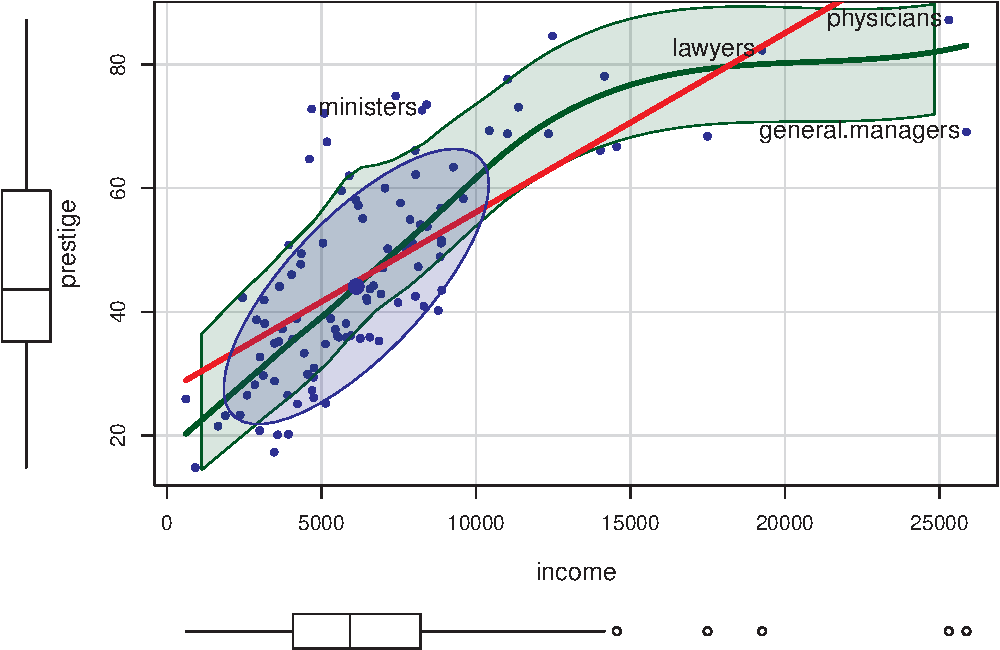
\includegraphics[width=0.8\textwidth,height=\textheight]{figs/ch03/fig-Prestige-scatterplot-income1-1.pdf}

}

\caption{\label{fig-Prestige-scatterplot-income1}Scatterplot of prestige
vs.~income, showing the linear regression line (\textcolor{red}{red}),
the loess smooth with a confidence envelope
(\textcolor{darkgreen}{darkgreen}) and a 68\% data ellipse. Points with
the 4 largest \(D^2\) values are labeled.}

\end{figure}%

There is a lot that can be seen here:

\begin{itemize}
\tightlist
\item
  \texttt{income} is positively skewed, as is often the case.
\item
  The loess smooth, on the scale of income, shows \texttt{prestige}
  increasing up to \$15,000 (these are 1971 incomes), and then leveling
  off.
\item
  The data ellipse, centered at the means encloses approximately 68\% of
  the data points. It adds visual information about the correlation and
  precision of the linear regression; but here, the non-linear trend for
  higher incomes strongly suggests a different approach.
\item
  The four points identified by their labels are those with the largest
  Mahalanobis distances. \texttt{scatterplot()} prints their labels to
  the console.
\end{itemize}

Figure~\ref{fig-Prestige-scatterplot-educ1} shows a similar plot for
education, which from the boxplot appears to be reasonably symmetric.
The smoothed curve is quite close to the linear regression, according to
which \texttt{prestige} increases on average
\texttt{coef(lm(prestige\ \textasciitilde{}\ education,\ data=Prestige)){[}"education"{]}}
= 5.361 with each year of education.

\begin{Shaded}
\begin{Highlighting}[]
\FunctionTok{scatterplot}\NormalTok{(prestige }\SpecialCharTok{\textasciitilde{}}\NormalTok{ education, }\AttributeTok{data=}\NormalTok{Prestige,}
  \AttributeTok{pch =} \DecValTok{16}\NormalTok{, }\AttributeTok{cex.lab =} \FloatTok{1.25}\NormalTok{,}
  \AttributeTok{regLine =} \FunctionTok{list}\NormalTok{(}\AttributeTok{col =} \StringTok{"red"}\NormalTok{, }\AttributeTok{lwd=}\DecValTok{3}\NormalTok{),}
  \AttributeTok{smooth =} \FunctionTok{list}\NormalTok{(}\AttributeTok{smoother=}\NormalTok{loessLine, }
                \AttributeTok{lty.smooth =} \DecValTok{1}\NormalTok{, }\AttributeTok{lwd.smooth=}\DecValTok{3}\NormalTok{,}
                \AttributeTok{col.smooth =} \StringTok{"darkgreen"}\NormalTok{, }
                \AttributeTok{col.var =} \StringTok{"darkgreen"}\NormalTok{),}
  \AttributeTok{ellipse =} \FunctionTok{list}\NormalTok{(}\AttributeTok{levels =} \FloatTok{0.68}\NormalTok{),}
  \AttributeTok{id =} \FunctionTok{list}\NormalTok{(}\AttributeTok{n=}\DecValTok{4}\NormalTok{, }\AttributeTok{method =} \StringTok{"mahal"}\NormalTok{, }\AttributeTok{col=}\StringTok{"black"}\NormalTok{, }\AttributeTok{cex=}\FloatTok{1.2}\NormalTok{))}
\CommentTok{\#\textgreater{}  physicians file.clerks    newsboys     farmers }
\CommentTok{\#\textgreater{}          24          41          53          67}
\end{Highlighting}
\end{Shaded}

\begin{figure}

\centering{

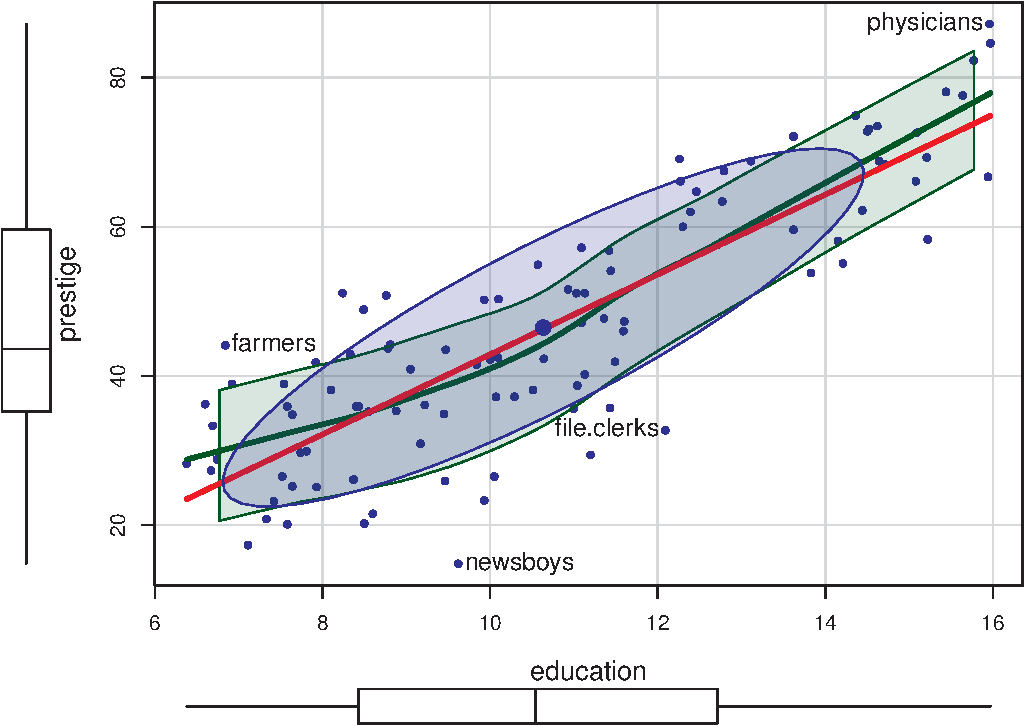
\includegraphics[width=0.8\textwidth,height=\textheight]{figs/ch03/fig-Prestige-scatterplot-educ1-1.pdf}

}

\caption{\label{fig-Prestige-scatterplot-educ1}Scatterplot of prestige
vs.~education, showing the linear regression line
(\textcolor{red}{red}), the loess smooth with a confidence envelope
(\textcolor{darkgreen}{darkgreen}) and a 68\% data ellipse.}

\end{figure}%

In this plot, farmers, newsboys, file.clerks and physicians are
identified as noteworthy, for being furthest from the mean by
Mahalanobis distance. In relation to their typical level of education,
these are mostly understandable, but it is nice that farmers are rated
of higher prestige than their level of education would predict.

Note that the \texttt{method} argument for point identification can take
a vector of case numbers indicating the points to be labeled. So, to
label the observations with large absolute standardized residuals in the
linear model \texttt{m}, you can use
\texttt{method\ =\ which(abs(rstandard(m))\ \textgreater{}\ 2)}.

\begin{Shaded}
\begin{Highlighting}[]
\NormalTok{m }\OtherTok{\textless{}{-}} \FunctionTok{lm}\NormalTok{(prestige }\SpecialCharTok{\textasciitilde{}}\NormalTok{ education, }\AttributeTok{data=}\NormalTok{Prestige)}
\FunctionTok{scatterplot}\NormalTok{(prestige }\SpecialCharTok{\textasciitilde{}}\NormalTok{ education, }\AttributeTok{data=}\NormalTok{Prestige,}
            \AttributeTok{pch =} \DecValTok{16}\NormalTok{, }\AttributeTok{cex.lab =} \FloatTok{1.25}\NormalTok{,}
            \AttributeTok{boxplots =} \ConstantTok{FALSE}\NormalTok{,}
            \AttributeTok{regLine =} \FunctionTok{list}\NormalTok{(}\AttributeTok{col =} \StringTok{"red"}\NormalTok{, }\AttributeTok{lwd=}\DecValTok{3}\NormalTok{),}
            \AttributeTok{smooth =} \FunctionTok{list}\NormalTok{(}\AttributeTok{smoother=}\NormalTok{loessLine,}
                          \AttributeTok{lty.smooth =} \DecValTok{1}\NormalTok{, }\AttributeTok{lwd.smooth=}\DecValTok{3}\NormalTok{,}
                          \AttributeTok{col.smooth =} \StringTok{"black"}\NormalTok{, }
                          \AttributeTok{col.var =} \StringTok{"darkgreen"}\NormalTok{),}
            \AttributeTok{ellipse =} \FunctionTok{list}\NormalTok{(}\AttributeTok{levels =} \FloatTok{0.68}\NormalTok{),}
            \AttributeTok{id =} \FunctionTok{list}\NormalTok{(}\AttributeTok{n=}\DecValTok{4}\NormalTok{, }\AttributeTok{method =} \FunctionTok{which}\NormalTok{(}\FunctionTok{abs}\NormalTok{(}\FunctionTok{rstandard}\NormalTok{(m))}\SpecialCharTok{\textgreater{}}\DecValTok{2}\NormalTok{), }
                      \AttributeTok{col=}\StringTok{"black"}\NormalTok{, }\AttributeTok{cex=}\FloatTok{1.2}\NormalTok{)) }\SpecialCharTok{|\textgreater{}} \FunctionTok{invisible}\NormalTok{()}
\end{Highlighting}
\end{Shaded}

\begin{figure}

\centering{

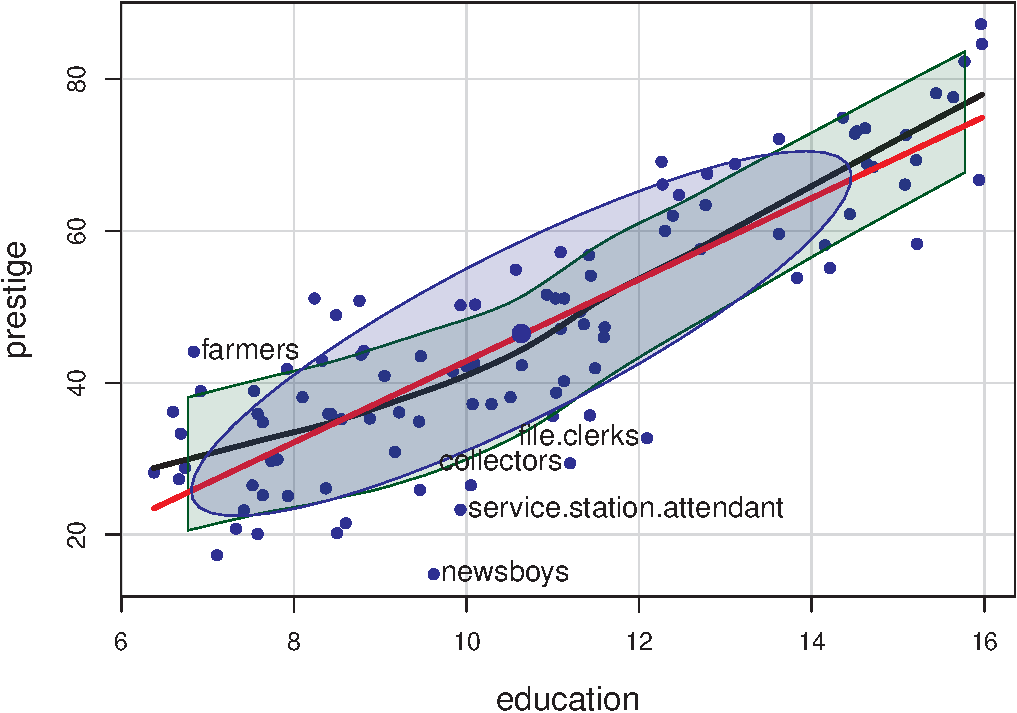
\includegraphics[width=0.8\textwidth,height=\textheight]{figs/ch03/fig-Prestige-scatterplot-educ2-1.pdf}

}

\caption{\label{fig-Prestige-scatterplot-educ2}Scatterplot of prestige
vs.~education, labeling points whose absolute standardized residual is
\textgreater{} 2.}

\end{figure}%

\subsubsection{Plotting on a log scale}\label{sec-log-scale}

A typical remedy for the non-linear relationship of income to prestige
is to plot income on a log scale. This usually makes sense, and
expresses a belief that a \textbf{multiple} of or \textbf{percentage
increase} in income has a constant impact on prestige, as opposed to the
\textbf{additive} interpretation for income itself.

For example, the slope of the linear regression line in
Figure~\ref{fig-Prestige-scatterplot-income1} is given by
\texttt{coef(lm(prestige\ \textasciitilde{}\ income,\ data=Prestige)){[}"income"{]}}
= 0.003. Multiplying this by 1000 says that a \$1000 increase in
\texttt{income} is associated with with an average increase of
\texttt{prestige} of 2.9.

In the plot below, \texttt{scatterplot(...,\ log\ =\ "x")} re-scales the
x-axis to the \(\log_e()\) scale. The slope,
\texttt{coef(lm(prestige\ \textasciitilde{}\ log(income),\ data=Prestige)){[}"log(income)"{]}}
= 21.556 says that a 1\% increase in salary is associated with an
average change of 21.55 / 100 in prestige.

\begin{Shaded}
\begin{Highlighting}[]
\FunctionTok{scatterplot}\NormalTok{(prestige }\SpecialCharTok{\textasciitilde{}}\NormalTok{ income, }\AttributeTok{data=}\NormalTok{Prestige,}
  \AttributeTok{log =} \StringTok{"x"}\NormalTok{,}
  \AttributeTok{pch =} \DecValTok{16}\NormalTok{, }\AttributeTok{cex.lab =} \FloatTok{1.25}\NormalTok{,}
  \AttributeTok{regLine =} \FunctionTok{list}\NormalTok{(}\AttributeTok{col =} \StringTok{"red"}\NormalTok{, }\AttributeTok{lwd=}\DecValTok{3}\NormalTok{),}
  \AttributeTok{smooth =} \FunctionTok{list}\NormalTok{(}\AttributeTok{smoother=}\NormalTok{loessLine,}
                \AttributeTok{lty.smooth =} \DecValTok{1}\NormalTok{, }\AttributeTok{lwd.smooth=}\DecValTok{3}\NormalTok{,}
                \AttributeTok{col.smooth =} \StringTok{"darkgreen"}\NormalTok{, }\AttributeTok{col.var =} \StringTok{"darkgreen"}\NormalTok{),}
  \AttributeTok{ellipse =} \FunctionTok{list}\NormalTok{(}\AttributeTok{levels =} \FloatTok{0.68}\NormalTok{),}
  \AttributeTok{id =} \FunctionTok{list}\NormalTok{(}\AttributeTok{n=}\DecValTok{4}\NormalTok{, }\AttributeTok{method =} \StringTok{"mahal"}\NormalTok{, }\AttributeTok{col=}\StringTok{"black"}\NormalTok{, }\AttributeTok{cex=}\FloatTok{1.2}\NormalTok{))}
\CommentTok{\#\textgreater{} general.managers        ministers         newsboys      babysitters }
\CommentTok{\#\textgreater{}                2               20               53               63}
\end{Highlighting}
\end{Shaded}

\begin{figure}

\centering{

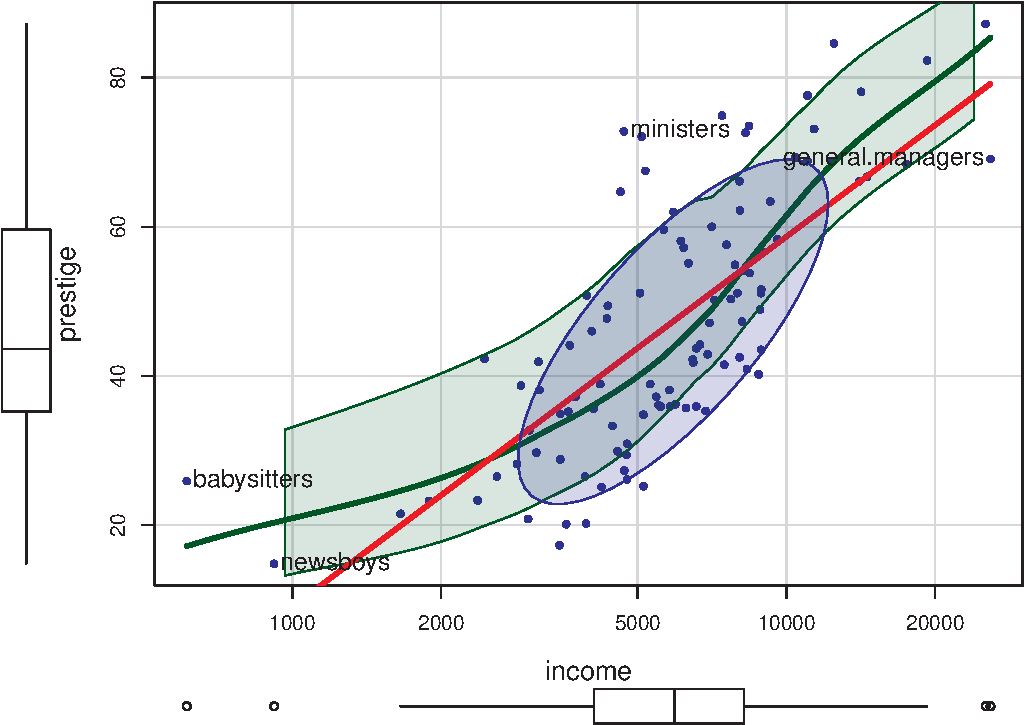
\includegraphics[width=0.8\textwidth,height=\textheight]{figs/ch03/fig-Prestige-scatterplot2-1.pdf}

}

\caption{\label{fig-Prestige-scatterplot2}Scatterplot of prestige
vs.~log(income).}

\end{figure}%

The smoothed curve in Figure~\ref{fig-Prestige-scatterplot2} exhibits a
slight tendency to bend upwards, but a linear relation is a reasonable
approximation.

\subsubsection{Stratifying}\label{sec-stratifying}

Before going further, it is instructive to ask what we could see in the
relationship between income and prestige if we stratified by type of
occupation, fitting separate regressions and smooths for blue collar,
white collar and professional incumbents in these occupations.

The formula
\texttt{prestige\ \textasciitilde{}\ income\ \textbar{}\ type} (read:
income \emph{given} type) is a natural way to specify grouping by
\texttt{type}; separate linear regressions and smooths are calculated
for each group, applying the color and point shapes specified by the
\texttt{col} and \texttt{pch} arguments.

\begin{Shaded}
\begin{Highlighting}[]
\FunctionTok{scatterplot}\NormalTok{(prestige }\SpecialCharTok{\textasciitilde{}}\NormalTok{ income }\SpecialCharTok{|}\NormalTok{ type, }\AttributeTok{data=}\NormalTok{Prestige,}
  \AttributeTok{col =} \FunctionTok{c}\NormalTok{(}\StringTok{"blue"}\NormalTok{, }\StringTok{"red"}\NormalTok{, }\StringTok{"darkgreen"}\NormalTok{),}
  \AttributeTok{pch =} \DecValTok{15}\SpecialCharTok{:}\DecValTok{17}\NormalTok{,}
  \AttributeTok{grid =} \ConstantTok{FALSE}\NormalTok{,}
  \AttributeTok{legend =} \FunctionTok{list}\NormalTok{(}\AttributeTok{coords=}\StringTok{"bottomright"}\NormalTok{),}
  \AttributeTok{regLine =} \FunctionTok{list}\NormalTok{(}\AttributeTok{lwd=}\DecValTok{3}\NormalTok{),}
  \AttributeTok{smooth=}\FunctionTok{list}\NormalTok{(}\AttributeTok{smoother=}\NormalTok{loessLine, }
              \AttributeTok{var=}\ConstantTok{FALSE}\NormalTok{, }\AttributeTok{lwd.smooth=}\DecValTok{2}\NormalTok{, }\AttributeTok{lty.smooth=}\DecValTok{1}\NormalTok{))}
\end{Highlighting}
\end{Shaded}

\begin{figure}[H]

\centering{

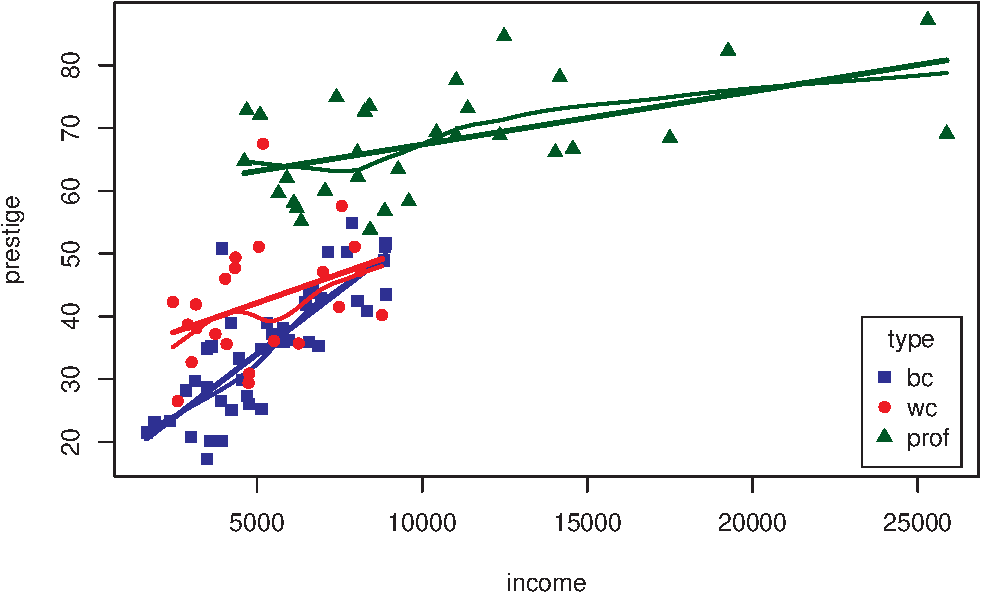
\includegraphics[width=0.8\textwidth,height=\textheight]{figs/ch03/fig-Prestige-scatterplot3-1.pdf}

}

\caption{\label{fig-Prestige-scatterplot3}Scatterplot of prestige
vs.~income, stratified by occupational type. This implies a different
interpretation, where occupation type is a moderator variable.}

\end{figure}%

This visual analysis offers a different interpretation of the dependence
of prestige on income, which appeared to be non-linear when occupation
type was ignored. Instead, Figure~\ref{fig-Prestige-scatterplot3}
suggests an \emph{interaction} of income by type. In a model formula
this would be expressed as one of:

\begin{Shaded}
\begin{Highlighting}[]
\FunctionTok{lm}\NormalTok{(prestige }\SpecialCharTok{\textasciitilde{}}\NormalTok{ income }\SpecialCharTok{+}\NormalTok{ type }\SpecialCharTok{+}\NormalTok{ income}\SpecialCharTok{:}\NormalTok{type, }\AttributeTok{data =}\NormalTok{ Prestige)}
\FunctionTok{lm}\NormalTok{(prestige }\SpecialCharTok{\textasciitilde{}}\NormalTok{ income }\SpecialCharTok{*}\NormalTok{ type, }\AttributeTok{data =}\NormalTok{ Prestige)}
\end{Highlighting}
\end{Shaded}

These models signify that there are different slopes (and intercepts)
for the three occupational types. In this interpretation, \texttt{type}
is a moderator variable, with a different story. The slopes of the
fitted lines suggest that among blue collar workers, prestige increases
sharply with their income. For white collar and professional workers,
there is still an increasing relation of prestige with income, but the
effect of income (slope) diminishes with higher occupational category. A
different plot entails a different story.

\subsection{Example: Penguins data}\label{sec-penguins}

\begin{figure}

\centering{

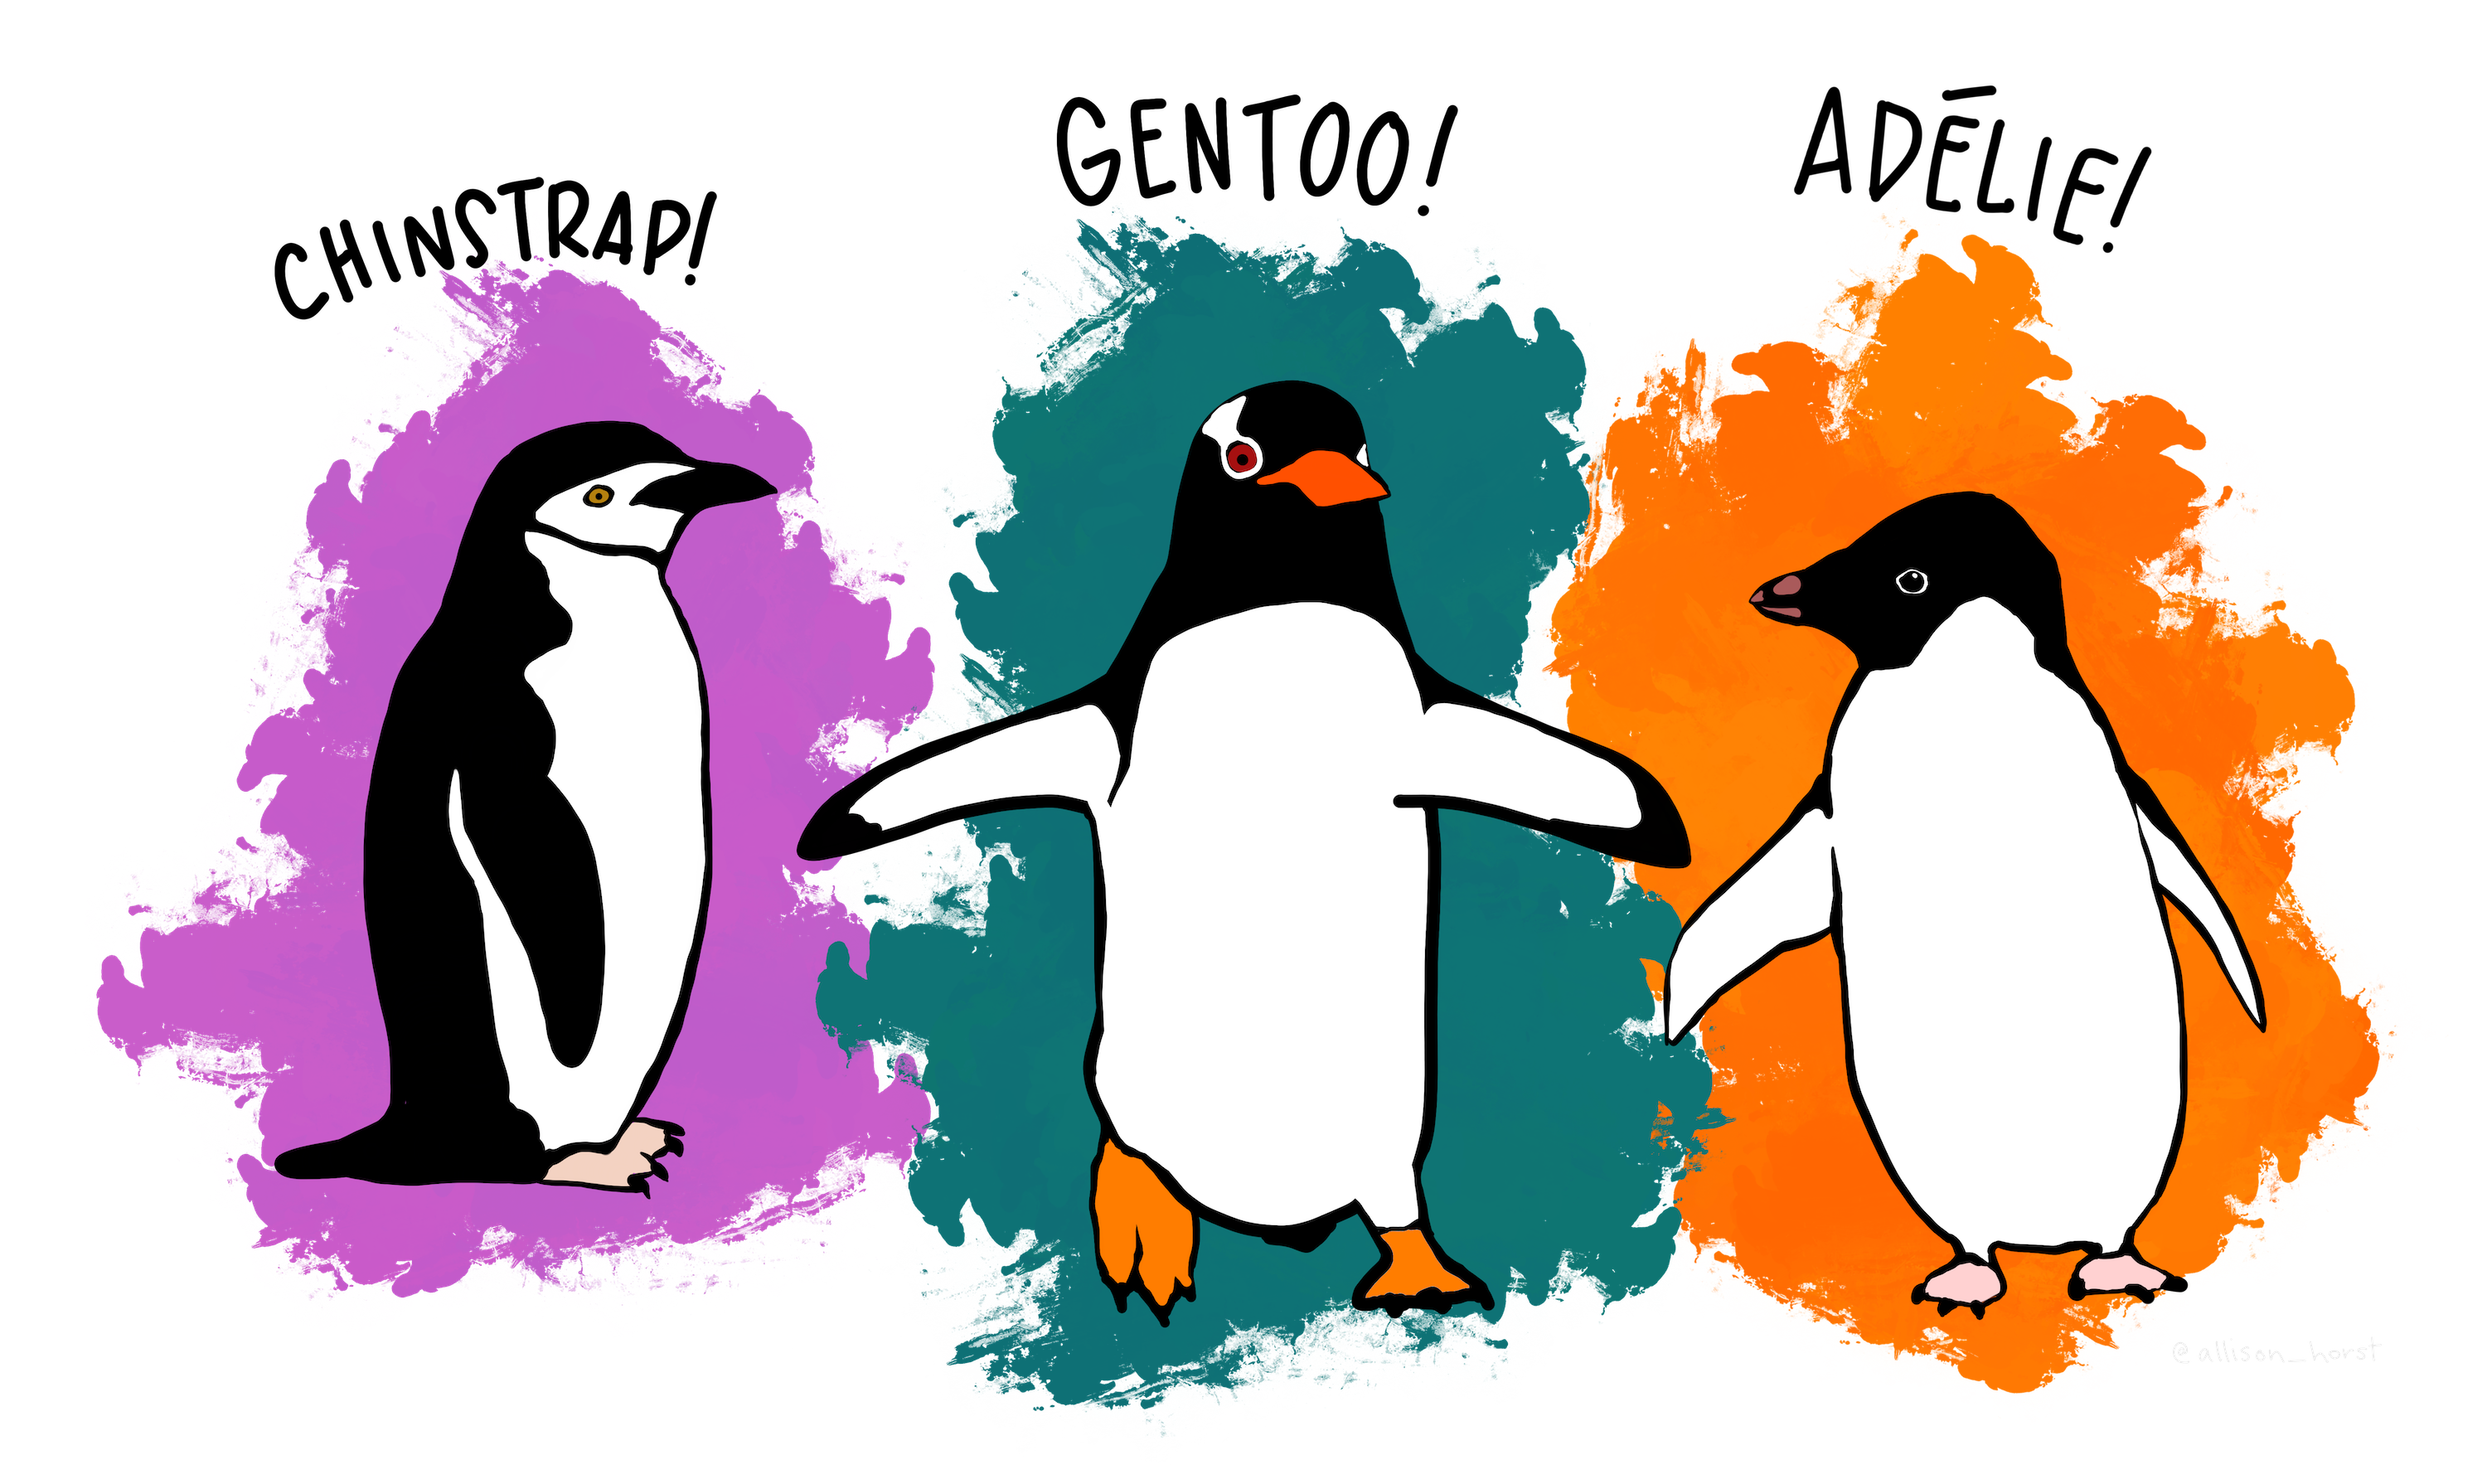
\includegraphics[width=0.8\textwidth,height=\textheight]{images/penguins-horst.png}

}

\caption{\label{fig-penguin-species}Penguin species observed in the
Palmer Archipelago. This is a cartoon, but it illustrates some features
of penguin body size measurements, and the colors typically used for
species. Image: Allison Horst}

\end{figure}%

The \texttt{penguins} dataset from the \textbf{palmerpenguins} package
(\citeproc{ref-R-palmerpenguins}{Horst et al., 2022}) provides further
instructive examples of plots and analyses of multivariate data. The
data consists of measurements of body size (flipper length, body mass,
bill length and depth) of 344 penguins collected at the
\href{https://pallter.marine.rutgers.edu/}{Palmer Research Station} in
Antarctica.

There were three different species of penguins (Adélie, Chinstrap \&
Gentoo) collected from 3 islands in the Palmer Archipelago between
2007--2009 (\citeproc{ref-Gorman2014}{Gorman et al., 2014}). The purpose
was to examine differences in size or appearance of these species,
particularly differences among the sexes (sexual dimorphism) in relation
to foraging and habitat.

Here, I use a slightly altered version of the dataset, \texttt{peng},
renaming variables to remove the units, making factors of character
variables and deleting a few cases with missing data.

\begin{Shaded}
\begin{Highlighting}[]
\FunctionTok{data}\NormalTok{(penguins, }\AttributeTok{package =} \StringTok{"palmerpenguins"}\NormalTok{)}
\NormalTok{peng }\OtherTok{\textless{}{-}}\NormalTok{ penguins }\SpecialCharTok{|\textgreater{}}
  \FunctionTok{rename}\NormalTok{(}
    \AttributeTok{bill\_length =}\NormalTok{ bill\_length\_mm, }
    \AttributeTok{bill\_depth =}\NormalTok{ bill\_depth\_mm, }
    \AttributeTok{flipper\_length =}\NormalTok{ flipper\_length\_mm, }
    \AttributeTok{body\_mass =}\NormalTok{ body\_mass\_g}
\NormalTok{  ) }\SpecialCharTok{|\textgreater{}}
  \FunctionTok{mutate}\NormalTok{(}\AttributeTok{species =} \FunctionTok{as.factor}\NormalTok{(species),}
         \AttributeTok{island =} \FunctionTok{as.factor}\NormalTok{(island),}
         \AttributeTok{sex =} \FunctionTok{as.factor}\NormalTok{(}\FunctionTok{substr}\NormalTok{(sex,}\DecValTok{1}\NormalTok{,}\DecValTok{1}\NormalTok{))) }\SpecialCharTok{|\textgreater{}}
\NormalTok{  tidyr}\SpecialCharTok{::}\FunctionTok{drop\_na}\NormalTok{()}

\FunctionTok{str}\NormalTok{(peng)}
\CommentTok{\#\textgreater{} tibble [333 x 8] (S3: tbl\_df/tbl/data.frame)}
\CommentTok{\#\textgreater{}  $ species       : Factor w/ 3 levels "Adelie","Chinstrap",..: 1 1 1 1 1 1 1 1 1 1 ...}
\CommentTok{\#\textgreater{}  $ island        : Factor w/ 3 levels "Biscoe","Dream",..: 3 3 3 3 3 3 3 3 3 3 ...}
\CommentTok{\#\textgreater{}  $ bill\_length   : num [1:333] 39.1 39.5 40.3 36.7 39.3 38.9 39.2 41.1 38.6 34.6 ...}
\CommentTok{\#\textgreater{}  $ bill\_depth    : num [1:333] 18.7 17.4 18 19.3 20.6 17.8 19.6 17.6 21.2 21.1 ...}
\CommentTok{\#\textgreater{}  $ flipper\_length: int [1:333] 181 186 195 193 190 181 195 182 191 198 ...}
\CommentTok{\#\textgreater{}  $ body\_mass     : int [1:333] 3750 3800 3250 3450 3650 3625 4675 3200 3800 4400 ...}
\CommentTok{\#\textgreater{}  $ sex           : Factor w/ 2 levels "f","m": 2 1 1 1 2 1 2 1 2 2 ...}
\CommentTok{\#\textgreater{}  $ year          : int [1:333] 2007 2007 2007 2007 2007 2007 2007 2007 2007 2007 ...}
\end{Highlighting}
\end{Shaded}

There are quite a few variables to choose for illustrating data ellipses
in scatterplots. Here I focus on the measures of their bills,
\texttt{bill\_length} and \texttt{bill\_depth} (indicating curvature)
and show how to use \texttt{ggplot2} for these plots.

I'll be using the penguins data quite a lot, so it is useful to set up
custom colors like those used in Figure~\ref{fig-penguin-species}, and
shown in Figure~\ref{fig-peng-colors} with their color codes. These are
shades of:

\begin{itemize}
\tightlist
\item
  \textcolor{orange}{Adelie}: \textcolor{orange}{orange},
\item
  \textcolor{purple}{Chinstrap}: \textcolor{purple}{purple}, and
\item
  \textcolor{green}{Gentoo}: \textcolor{green}{green}.
\end{itemize}

\begin{figure}

\centering{

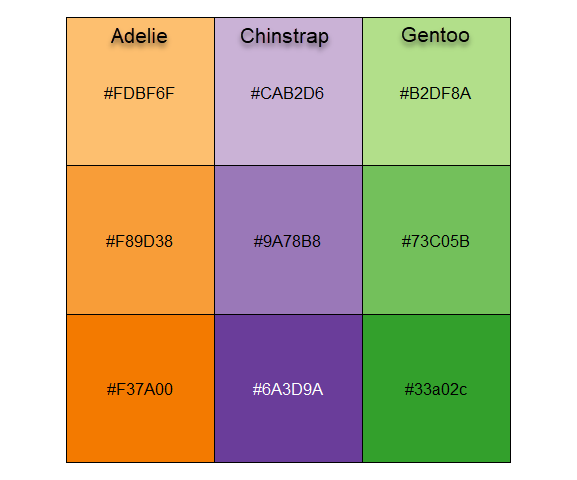
\includegraphics[width=0.7\textwidth,height=\textheight]{images/peng-colors.png}

}

\caption{\label{fig-peng-colors}Color palettes used for penguin
species.}

\end{figure}%

To use these in \texttt{ggplot2} I define a function
\texttt{peng.colors()} that allows shades of light, medium and dark and
then functions \texttt{scale\_*\_penguins()} for color and fill.

\begin{Shaded}
\begin{Highlighting}[]
\NormalTok{peng.colors }\OtherTok{\textless{}{-}} \ControlFlowTok{function}\NormalTok{(}\AttributeTok{shade=}\FunctionTok{c}\NormalTok{(}\StringTok{"medium"}\NormalTok{, }\StringTok{"light"}\NormalTok{, }\StringTok{"dark"}\NormalTok{)) \{}
\NormalTok{  shade }\OtherTok{=} \FunctionTok{match.arg}\NormalTok{(shade)}
  \CommentTok{\#             light      medium     dark}
\NormalTok{  oranges }\OtherTok{\textless{}{-}} \FunctionTok{c}\NormalTok{(}\StringTok{"\#FDBF6F"}\NormalTok{, }\StringTok{"\#F89D38"}\NormalTok{, }\StringTok{"\#F37A00"}\NormalTok{)  }\CommentTok{\# Adelie}
\NormalTok{  purples }\OtherTok{\textless{}{-}} \FunctionTok{c}\NormalTok{(}\StringTok{"\#CAB2D6"}\NormalTok{, }\StringTok{"\#9A78B8"}\NormalTok{, }\StringTok{"\#6A3D9A"}\NormalTok{)  }\CommentTok{\# Chinstrap}
\NormalTok{  greens }\OtherTok{\textless{}{-}}  \FunctionTok{c}\NormalTok{(}\StringTok{"\#B2DF8A"}\NormalTok{, }\StringTok{"\#73C05B"}\NormalTok{, }\StringTok{"\#33a02c"}\NormalTok{)  }\CommentTok{\# Gentoo}
  
\NormalTok{  cols.vec }\OtherTok{\textless{}{-}} \FunctionTok{c}\NormalTok{(oranges, purples, greens)}
\NormalTok{  cols.mat }\OtherTok{\textless{}{-}} 
    \FunctionTok{matrix}\NormalTok{(cols.vec, }\DecValTok{3}\NormalTok{, }\DecValTok{3}\NormalTok{, }
           \AttributeTok{byrow =} \ConstantTok{TRUE}\NormalTok{,}
           \AttributeTok{dimnames =} \FunctionTok{list}\NormalTok{(}\AttributeTok{species =} \FunctionTok{c}\NormalTok{(}\StringTok{"Adelie"}\NormalTok{, }\StringTok{"Chinstrap"}\NormalTok{, }\StringTok{"Gentoo"}\NormalTok{),}
                           \AttributeTok{shade =} \FunctionTok{c}\NormalTok{(}\StringTok{"light"}\NormalTok{, }\StringTok{"medium"}\NormalTok{, }\StringTok{"dark"}\NormalTok{)))}
  \CommentTok{\# get shaded colors}
\NormalTok{  cols.mat[, shade ]}
\NormalTok{\}}

\CommentTok{\# define color and fill scales}
\NormalTok{scale\_fill\_penguins }\OtherTok{\textless{}{-}} \ControlFlowTok{function}\NormalTok{(}\AttributeTok{shade=}\FunctionTok{c}\NormalTok{(}\StringTok{"medium"}\NormalTok{, }\StringTok{"light"}\NormalTok{, }\StringTok{"dark"}\NormalTok{), ...)\{}
\NormalTok{  shade }\OtherTok{=} \FunctionTok{match.arg}\NormalTok{(shade)}
\NormalTok{  ggplot2}\SpecialCharTok{::}\FunctionTok{discrete\_scale}\NormalTok{(}
    \StringTok{"fill"}\NormalTok{,}\StringTok{"penguins"}\NormalTok{,}
\NormalTok{     scales}\SpecialCharTok{:::}\FunctionTok{manual\_pal}\NormalTok{(}\AttributeTok{values =} \FunctionTok{peng.colors}\NormalTok{(shade)), ...)}
\NormalTok{\}}

\NormalTok{scale\_colour\_penguins }\OtherTok{\textless{}{-}} \ControlFlowTok{function}\NormalTok{(}\AttributeTok{shade=}\FunctionTok{c}\NormalTok{(}\StringTok{"medium"}\NormalTok{, }\StringTok{"light"}\NormalTok{, }\StringTok{"dark"}\NormalTok{), ...)\{}
\NormalTok{  shade }\OtherTok{=} \FunctionTok{match.arg}\NormalTok{(shade)}
\NormalTok{  ggplot2}\SpecialCharTok{::}\FunctionTok{discrete\_scale}\NormalTok{(}
    \StringTok{"colour"}\NormalTok{,}\StringTok{"penguins"}\NormalTok{,}
\NormalTok{    scales}\SpecialCharTok{:::}\FunctionTok{manual\_pal}\NormalTok{(}\AttributeTok{values =} \FunctionTok{peng.colors}\NormalTok{(shade)), ...)}
\NormalTok{\}}
\NormalTok{scale\_color\_penguins }\OtherTok{\textless{}{-}}\NormalTok{ scale\_colour\_penguins}
\end{Highlighting}
\end{Shaded}

This is used to define a \texttt{theme\_penguins()} function that I use
to simply change the color and fill scales for plots below.

\begin{Shaded}
\begin{Highlighting}[]
\NormalTok{theme\_penguins }\OtherTok{\textless{}{-}} \ControlFlowTok{function}\NormalTok{(}\AttributeTok{shade=}\FunctionTok{c}\NormalTok{(}\StringTok{"medium"}\NormalTok{, }\StringTok{"light"}\NormalTok{, }\StringTok{"dark"}\NormalTok{), ...) \{}
\NormalTok{  shade }\OtherTok{=} \FunctionTok{match.arg}\NormalTok{(shade)}
  \FunctionTok{list}\NormalTok{(}\FunctionTok{scale\_color\_penguins}\NormalTok{(}\AttributeTok{shade=}\NormalTok{shade),}
       \FunctionTok{scale\_fill\_penguins}\NormalTok{(}\AttributeTok{shade=}\NormalTok{shade)}
\NormalTok{      )}
\NormalTok{\}}
\end{Highlighting}
\end{Shaded}

An initial plot using \texttt{ggplot2} shown in
Figure~\ref{fig-peng-ggplot1} uses color and point shape to distinguish
the three penguin species. I annotate the plot of points using the
linear regression lines, loess smooths to check for non-linearity and
95\% data ellipses to show precision of the linear relation.

\begin{Shaded}
\begin{Highlighting}[]
\FunctionTok{ggplot}\NormalTok{(peng, }
       \FunctionTok{aes}\NormalTok{(}\AttributeTok{x =}\NormalTok{ bill\_length, }\AttributeTok{y =}\NormalTok{ bill\_depth,}
           \AttributeTok{color =}\NormalTok{ species, }\AttributeTok{shape =}\NormalTok{ species, }\AttributeTok{fill=}\NormalTok{species)) }\SpecialCharTok{+}
  \FunctionTok{geom\_point}\NormalTok{(}\AttributeTok{size=}\DecValTok{2}\NormalTok{) }\SpecialCharTok{+}
  \FunctionTok{geom\_smooth}\NormalTok{(}\AttributeTok{method =} \StringTok{"lm"}\NormalTok{, }\AttributeTok{formula =}\NormalTok{ y }\SpecialCharTok{\textasciitilde{}}\NormalTok{ x,}
              \AttributeTok{se=}\ConstantTok{FALSE}\NormalTok{, }\AttributeTok{linewidth=}\DecValTok{2}\NormalTok{) }\SpecialCharTok{+}
  \FunctionTok{geom\_smooth}\NormalTok{(}\AttributeTok{method =} \StringTok{"loess"}\NormalTok{,  }\AttributeTok{formula =}\NormalTok{ y }\SpecialCharTok{\textasciitilde{}}\NormalTok{ x,}
              \AttributeTok{linewidth =} \FloatTok{1.5}\NormalTok{, }\AttributeTok{se =} \ConstantTok{FALSE}\NormalTok{, }\AttributeTok{alpha=}\FloatTok{0.1}\NormalTok{) }\SpecialCharTok{+}
  \FunctionTok{stat\_ellipse}\NormalTok{(}\AttributeTok{geom =} \StringTok{"polygon"}\NormalTok{, }\AttributeTok{level =} \FloatTok{0.95}\NormalTok{, }\AttributeTok{alpha =} \FloatTok{0.2}\NormalTok{) }\SpecialCharTok{+}
  \FunctionTok{theme\_penguins}\NormalTok{(}\StringTok{"dark"}\NormalTok{) }\SpecialCharTok{+}
  \FunctionTok{theme}\NormalTok{(}\AttributeTok{legend.position =} \StringTok{"inside"}\NormalTok{,}
        \AttributeTok{legend.position.inside =} \FunctionTok{c}\NormalTok{(}\FloatTok{0.85}\NormalTok{, }\FloatTok{0.15}\NormalTok{))}
\end{Highlighting}
\end{Shaded}

\begin{figure}[H]

\centering{

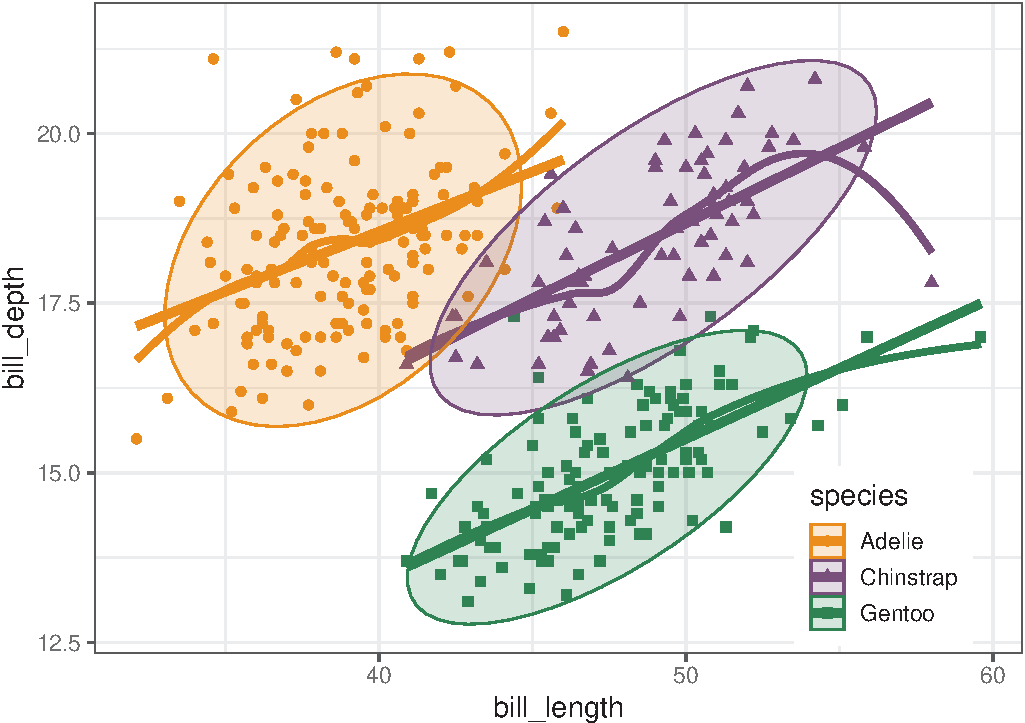
\includegraphics[width=0.8\textwidth,height=\textheight]{figs/ch03/fig-peng-ggplot1-1.pdf}

}

\caption{\label{fig-peng-ggplot1}Penguin bill length and bill depth
according to species.}

\end{figure}%

Overall, the three species occupy different regions of this 2D space and
for each species the relation between bill length and depth appears
reasonably linear. Given this, we can suppress plotting the data points
to get a visual summary of the data using the fitted regression lines
and data ellipses, as shown in Figure~\ref{fig-peng-ggplot2}.

This idea, of \textbf{visual thinning} a graph to focus on what should
be seen, becomes increasingly useful as the data becomes more complex.
The \texttt{ggplot2} framework encourages this, because we can think of
various components as layers, to be included or not. Here I chose to
include only the regression line and add data ellipses of 40\%, 68\% and
95\% coverage to highlight the increasing bivariate density around the
group means.

\begin{Shaded}
\begin{Highlighting}[]
\FunctionTok{ggplot}\NormalTok{(peng, }
       \FunctionTok{aes}\NormalTok{(}\AttributeTok{x =}\NormalTok{ bill\_length, }\AttributeTok{y =}\NormalTok{ bill\_depth,}
           \AttributeTok{color =}\NormalTok{ species, }\AttributeTok{shape =}\NormalTok{ species, }\AttributeTok{fill=}\NormalTok{species)) }\SpecialCharTok{+}
  \FunctionTok{geom\_smooth}\NormalTok{(}\AttributeTok{method =} \StringTok{"lm"}\NormalTok{,  }\AttributeTok{se=}\ConstantTok{FALSE}\NormalTok{, }\AttributeTok{linewidth=}\DecValTok{2}\NormalTok{) }\SpecialCharTok{+}
  \FunctionTok{stat\_ellipse}\NormalTok{(}\AttributeTok{geom =} \StringTok{"polygon"}\NormalTok{, }\AttributeTok{level =} \FloatTok{0.95}\NormalTok{, }\AttributeTok{alpha =} \FloatTok{0.2}\NormalTok{) }\SpecialCharTok{+}
  \FunctionTok{stat\_ellipse}\NormalTok{(}\AttributeTok{geom =} \StringTok{"polygon"}\NormalTok{, }\AttributeTok{level =} \FloatTok{0.68}\NormalTok{, }\AttributeTok{alpha =} \FloatTok{0.2}\NormalTok{) }\SpecialCharTok{+}
  \FunctionTok{stat\_ellipse}\NormalTok{(}\AttributeTok{geom =} \StringTok{"polygon"}\NormalTok{, }\AttributeTok{level =} \FloatTok{0.40}\NormalTok{, }\AttributeTok{alpha =} \FloatTok{0.2}\NormalTok{) }\SpecialCharTok{+}
  \FunctionTok{theme\_penguins}\NormalTok{(}\StringTok{"dark"}\NormalTok{) }\SpecialCharTok{+}
  \FunctionTok{theme}\NormalTok{(}\AttributeTok{legend.position =} \StringTok{"inside"}\NormalTok{,}
        \AttributeTok{legend.position.inside =} \FunctionTok{c}\NormalTok{(}\FloatTok{0.85}\NormalTok{, }\FloatTok{0.15}\NormalTok{))}
\end{Highlighting}
\end{Shaded}

\begin{figure}[H]

\centering{

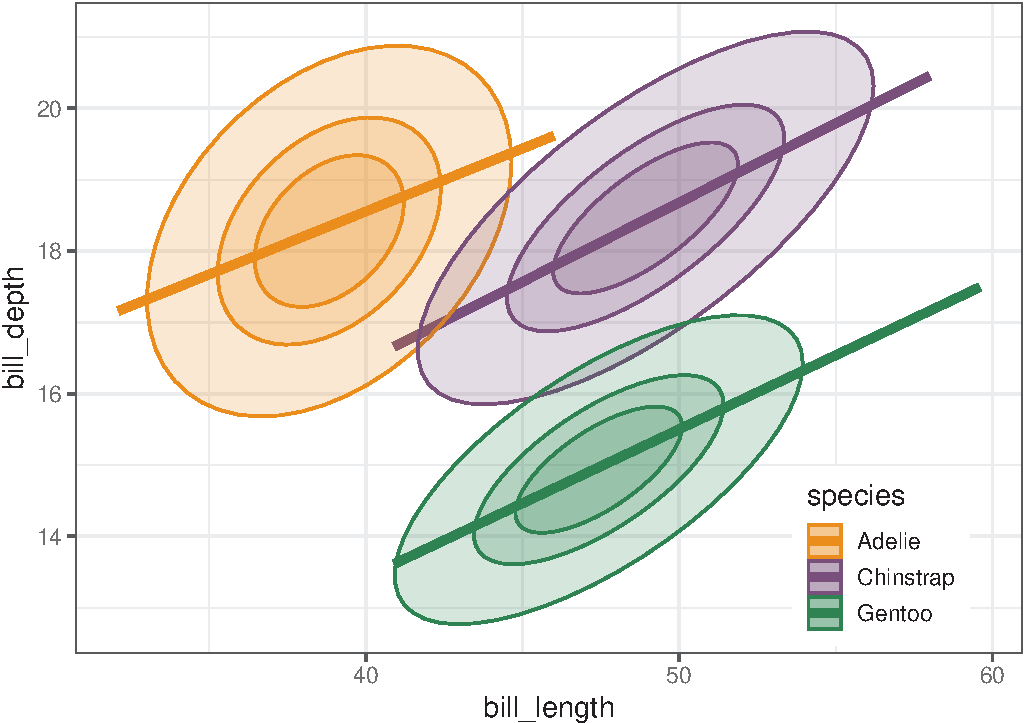
\includegraphics[width=0.8\textwidth,height=\textheight]{figs/ch03/fig-peng-ggplot2-1.pdf}

}

\caption{\label{fig-peng-ggplot2}\textbf{Visual thinning}: Suppressing
the data points gives a visual summary of the relation between bill
length and bill depth using the regression line and data ellipses.}

\end{figure}%

\subsubsection{Nonparamtric bivariate density
plots}\label{nonparamtric-bivariate-density-plots}

While I emphasize data ellipses (because I like their beautiful
geometry), other visual summaries of the bivariate density are possible
and often useful.

For a single variable, \texttt{stats::density()} and
\texttt{ggplot2::geom\_density()} calculate a smoothed estimate of the
density using nonparametric kernel methods
(\citeproc{ref-Silverman:86}{Silverman, 1986}) whose smoothness is
controlled by a bandwidth parameter, analogous to the span in a loess
smoother. This idea extends to two (and more) variables
(\citeproc{ref-Scott1992}{Scott, 1992}). For bivariate data,
\texttt{MASS::kde2d()} estimates the density on a square \(n \times n\)
grid over the ranges of the variables.

\texttt{ggplot2} provides \texttt{geom\_density\_2d()} which uses
\texttt{MASS::kde2d()} and displays these as contours--- horizontal
slices of the 3D surface at equally-spaced heights and projects these
onto the 2D plane. The \textbf{ggdensity} package
(\citeproc{ref-R-ggdensity}{Otto \& Kahle, 2023}) extends this with
\texttt{geom\_hdr()}, computing the high density regions that bound
given levels of probability and maps these to the \texttt{alpha}
transparency aesthetic. A \texttt{method} argument allows you to specify
various nonparametric (\texttt{method\ ="kde"} is the default) and
parametric (\texttt{method\ ="mvnorm"} gives normal data ellipses) ways
to estimate the underlying bivariate distribution.

Figure~\ref{fig-peng-ggdensity} shows these side-by-side for comparison.
With \texttt{geom\_density\_2d()} you can specify either the number of
contour \texttt{bins} or the width of these bins (\texttt{binwidth}).
For \texttt{geom\_hdr()}, the \texttt{probs} argument gives a result
that is easier to understand.

\begin{Shaded}
\begin{Highlighting}[]
\FunctionTok{library}\NormalTok{(ggdensity)}
\FunctionTok{library}\NormalTok{(patchwork)}
\NormalTok{p1 }\OtherTok{\textless{}{-}} \FunctionTok{ggplot}\NormalTok{(peng, }
       \FunctionTok{aes}\NormalTok{(}\AttributeTok{x =}\NormalTok{ bill\_length, }\AttributeTok{y =}\NormalTok{ bill\_depth,}
           \AttributeTok{color =}\NormalTok{ species)) }\SpecialCharTok{+}
  \FunctionTok{geom\_smooth}\NormalTok{(}\AttributeTok{method =} \StringTok{"lm"}\NormalTok{,  }\AttributeTok{se=}\ConstantTok{FALSE}\NormalTok{, }\AttributeTok{linewidth=}\DecValTok{2}\NormalTok{) }\SpecialCharTok{+}
  \FunctionTok{geom\_density\_2d}\NormalTok{(}\AttributeTok{linewidth =} \FloatTok{1.1}\NormalTok{, }\AttributeTok{bins =} \DecValTok{8}\NormalTok{) }\SpecialCharTok{+}
  \FunctionTok{ggtitle}\NormalTok{(}\StringTok{"geom\_density\_2d"}\NormalTok{) }\SpecialCharTok{+}
  \FunctionTok{theme\_bw}\NormalTok{(}\AttributeTok{base\_size =} \DecValTok{14}\NormalTok{) }\SpecialCharTok{+} 
  \FunctionTok{theme\_penguins}\NormalTok{() }\SpecialCharTok{+}
  \FunctionTok{theme}\NormalTok{(}\AttributeTok{legend.position =} \StringTok{"inside"}\NormalTok{,}
        \AttributeTok{legend.position.inside =} \FunctionTok{c}\NormalTok{(}\FloatTok{0.85}\NormalTok{, }\FloatTok{0.15}\NormalTok{))}

\NormalTok{p2 }\OtherTok{\textless{}{-}} \FunctionTok{ggplot}\NormalTok{(peng, }
       \FunctionTok{aes}\NormalTok{(}\AttributeTok{x =}\NormalTok{ bill\_length, }\AttributeTok{y =}\NormalTok{ bill\_depth,}
           \AttributeTok{color =}\NormalTok{ species, }\AttributeTok{fill =}\NormalTok{ species)) }\SpecialCharTok{+}
  \FunctionTok{geom\_smooth}\NormalTok{(}\AttributeTok{method =} \StringTok{"lm"}\NormalTok{,  }\AttributeTok{se=}\ConstantTok{FALSE}\NormalTok{, }\AttributeTok{linewidth=}\DecValTok{2}\NormalTok{) }\SpecialCharTok{+}
  \FunctionTok{geom\_hdr}\NormalTok{(}\AttributeTok{probs =} \FunctionTok{c}\NormalTok{(}\FloatTok{0.95}\NormalTok{, }\FloatTok{0.68}\NormalTok{, }\FloatTok{0.4}\NormalTok{), }\AttributeTok{show.legend =} \ConstantTok{FALSE}\NormalTok{) }\SpecialCharTok{+}
  \FunctionTok{ggtitle}\NormalTok{(}\StringTok{"ggdensity::geom\_hdr"}\NormalTok{) }\SpecialCharTok{+}
  \FunctionTok{theme\_bw}\NormalTok{(}\AttributeTok{base\_size =} \DecValTok{14}\NormalTok{) }\SpecialCharTok{+}
  \FunctionTok{theme\_penguins}\NormalTok{() }\SpecialCharTok{+}
  \FunctionTok{theme}\NormalTok{(}\AttributeTok{legend.position =} \StringTok{"none"}\NormalTok{)}

\NormalTok{p1 }\SpecialCharTok{+}\NormalTok{ p2}
\end{Highlighting}
\end{Shaded}

\begin{figure}[H]

\centering{

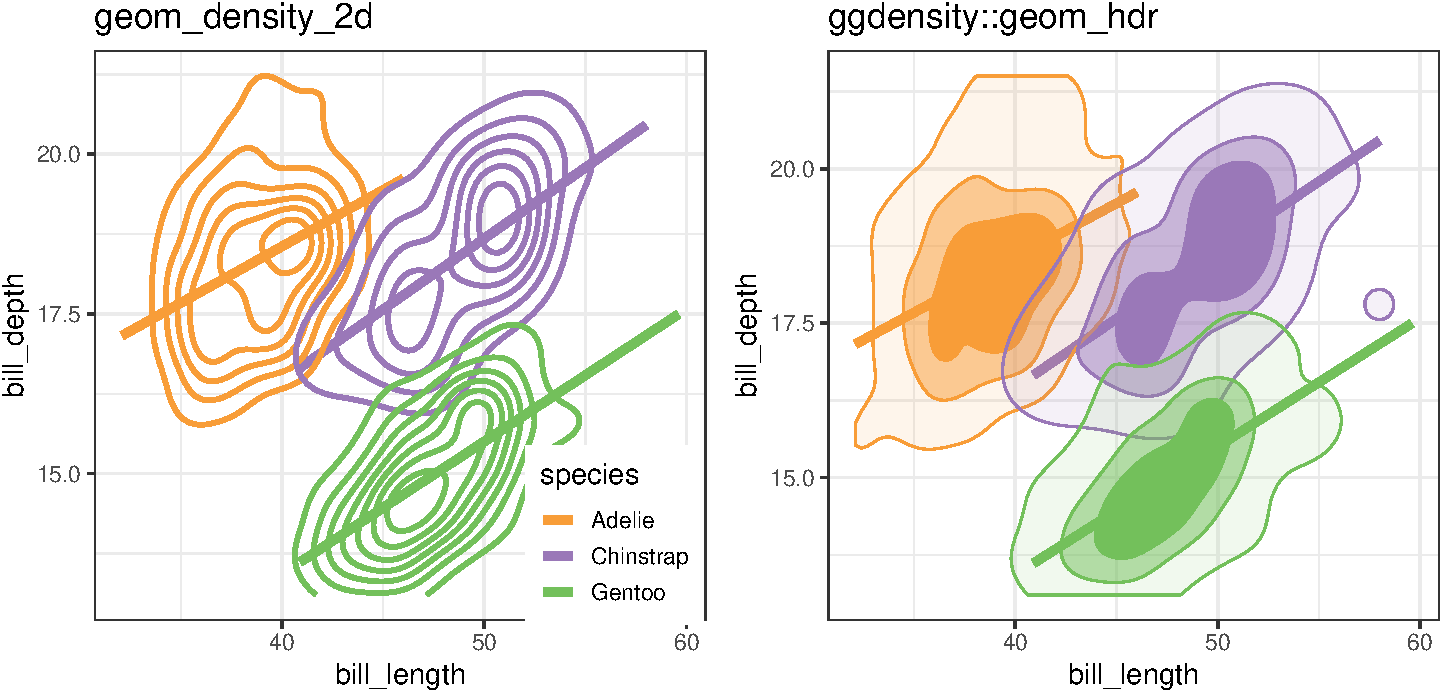
\includegraphics[width=1.2\textwidth,height=\textheight]{figs/ch03/fig-peng-ggdensity-1.pdf}

}

\caption{\label{fig-peng-ggdensity}\textbf{Bivariate densities} show the
contours of the 3D surface representing the frequency in the joint
distribution of bill length and bill depth.}

\end{figure}%

\subsection{Simpson's paradox: marginal and conditional
relationships}\label{simpsons-paradox-marginal-and-conditional-relationships}

Because it provides a visual representation of means, variances, and
correlations, the data ellipse is ideally suited as a tool for
illustrating and explicating various phenomena that occur in the
analysis of linear models. One class of simple, but important, examples
concerns the difference between the \emph{marginal relationship} between
variables, ignoring some important factor or covariate, and the
\emph{conditional} relationship, adjusting (controlling) for that
variable.

Simpson's (\citeproc{ref-Simpson:51}{1951}) paradox occurs when the
marginal and conditional relationships differ in direction. That is, the
overall correlation in a model \texttt{y\ \textasciitilde{}\ x} might be
negative, while the within-group correlations in separate models for
each group \texttt{y{[}g{]}\ \textasciitilde{}\ x{[}g{]}} might be
positive, or vice versa.

This may be seen in the plots of bill length against bill depth for the
penguin data shown in Figure~\ref{fig-peng-simpsons}. Ignoring penguin
species, the marginal, total-sample correlation is slightly negative as
seen in panel (a). The individual-sample ellipses in panel (b) show that
the conditional, within-species correlations are all positive, with
approximately equal regression slopes. However the group means have a
negative relationship, accounting for the negative marginal correlation
when species is ignored.

\begin{figure}

\centering{

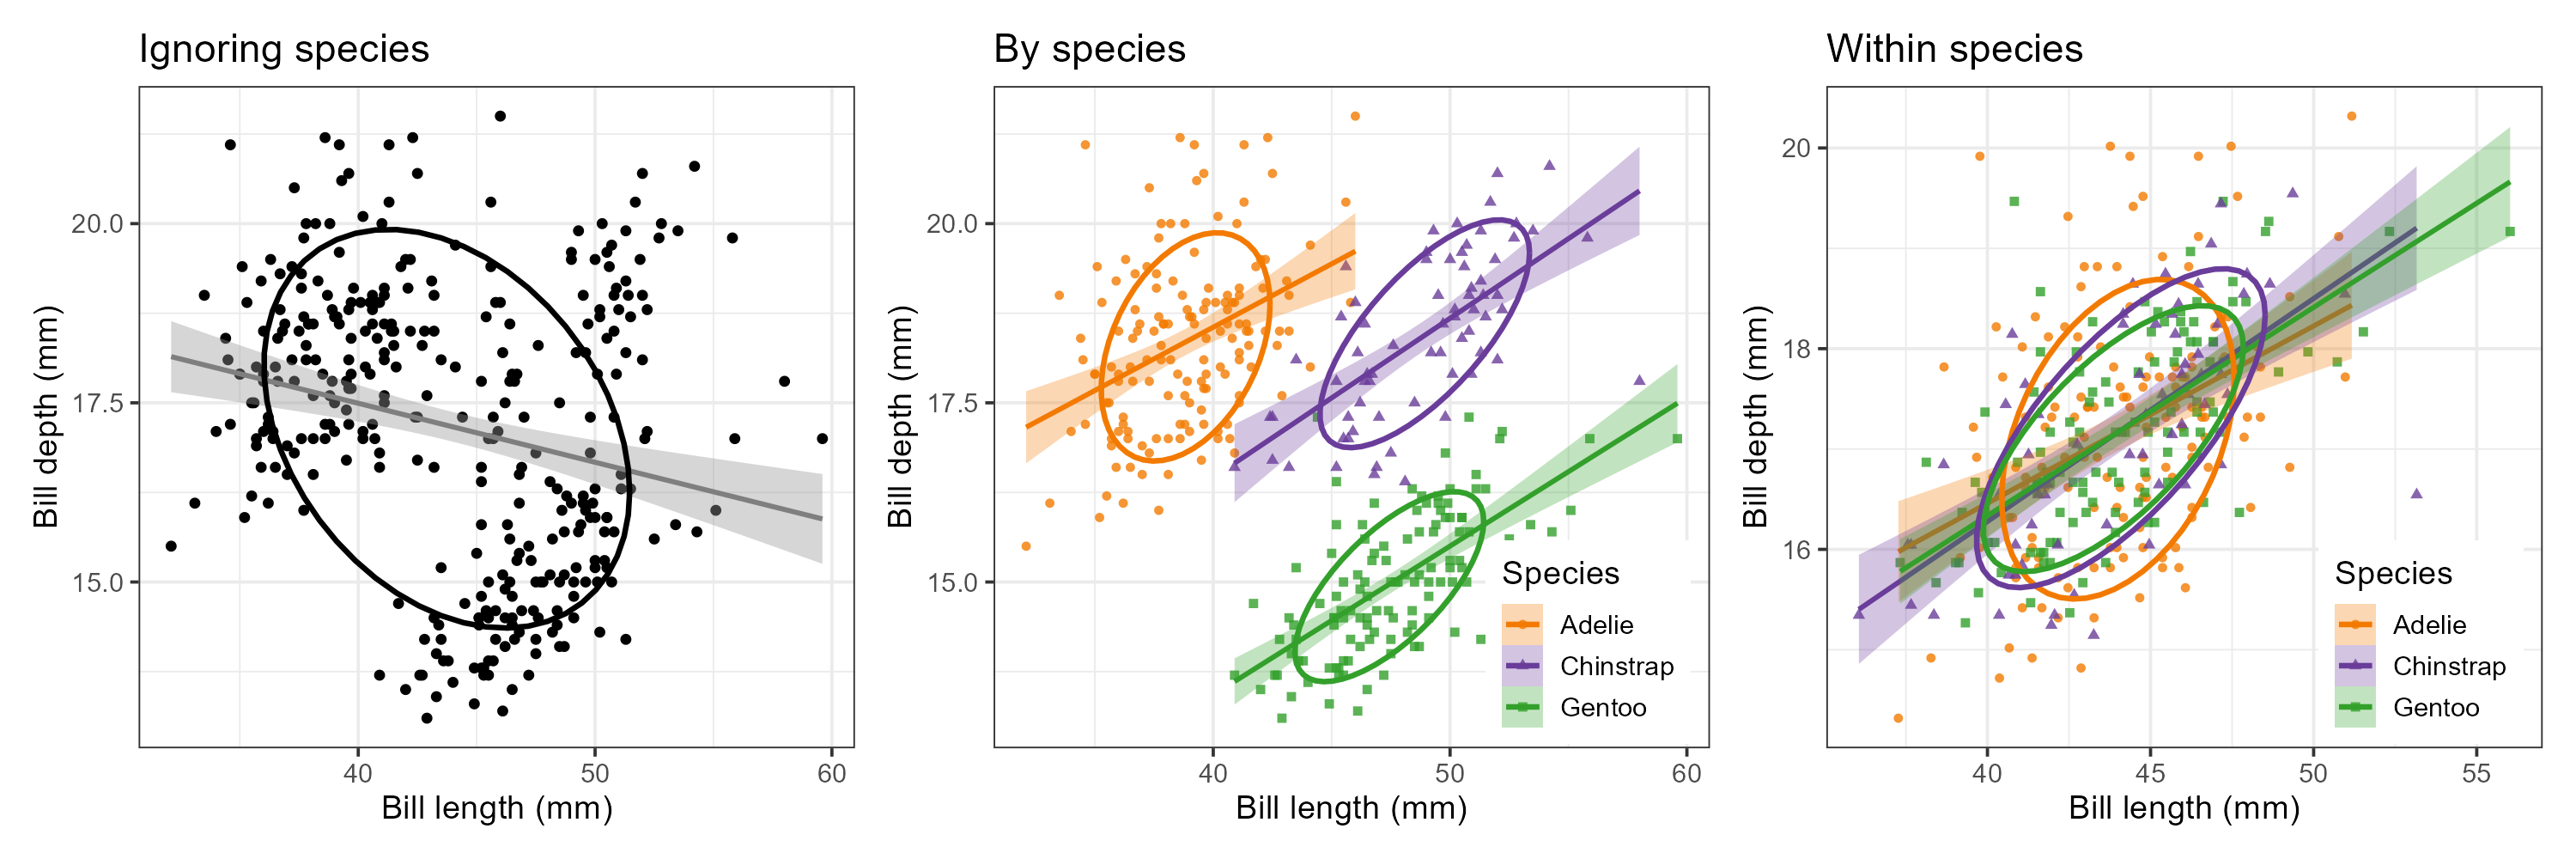
\includegraphics[width=1.2\textwidth,height=\textheight]{images/peng-simpsons.png}

}

\caption{\label{fig-peng-simpsons}Marginal (a), conditional (b), and
pooled within-sample (c) relationships of bill length and depth in the
Penguins data. Each plot shows the 68\% data ellipse and regression
line(s) with 95\% confidence bands.}

\end{figure}%

The regression line in panel (a) is that for the linear model
\texttt{lm(bill\_depth\ \textasciitilde{}\ bill\_length)}, while the
separate lines in panel (b) are those for the model
\texttt{lm(bill\_depth\ \textasciitilde{}\ bill\_length\ *\ species)}
which allows a different slope and intercept for each species.

A correct analysis of the (conditional) relationship between these
variables, controlling or adjusting for mean differences among species,
is based on the pooled within-sample covariance matrix, a weighted
average of the individual within-group \(\mathbf{S}_i\), \[
\mathbf{S}_{\textrm{within}}  =
\sum_{i=1}^g
(n_i - 1) \mathbf{S}_i \, / \, (N - g)
\:\: ,
\] where \(N = \sum n_i\). The result is shown in panel (c) of
Figure~\ref{fig-peng-simpsons}.

In this graph, the data for each species were first transformed to
deviations from the species means on both variables and then translated
back to the grand means. You can also see here that the shapes and sizes
of the individual data ellipses are roughly comparable, but perhaps not
identical. This visual idea of centering groups to a common mean will
become important in Chapter~\ref{sec-eqcov} when we want to test the
assumption of equality of error covariances in multivariate models.

The \texttt{ggplot2} code for the panels in this figure are shown below.
Note that for components that will be the same across panels, you can
define elements (e.g., \texttt{labels}, \texttt{theme\_penguins()},
\texttt{legend\_position}) once, and then re-use these across several
graphs.

\section{(a) Ignoring species}

\begin{Shaded}
\begin{Highlighting}[]
\NormalTok{labels }\OtherTok{\textless{}{-}} \FunctionTok{labs}\NormalTok{(}
  \AttributeTok{x =} \StringTok{"Bill length (mm)"}\NormalTok{,}
  \AttributeTok{y =} \StringTok{"Bill depth (mm)"}\NormalTok{,}
  \AttributeTok{color =} \StringTok{"Species"}\NormalTok{,}
  \AttributeTok{shape =} \StringTok{"Species"}\NormalTok{,}
  \AttributeTok{fill =} \StringTok{"Species"}\NormalTok{) }

\NormalTok{plt1 }\OtherTok{\textless{}{-}} \FunctionTok{ggplot}\NormalTok{(}\AttributeTok{data =}\NormalTok{ peng,}
               \FunctionTok{aes}\NormalTok{(}\AttributeTok{x =}\NormalTok{ bill\_length,}
                   \AttributeTok{y =}\NormalTok{ bill\_depth)) }\SpecialCharTok{+}
  \FunctionTok{geom\_point}\NormalTok{(}\AttributeTok{size =} \FloatTok{1.5}\NormalTok{) }\SpecialCharTok{+}
  \FunctionTok{geom\_smooth}\NormalTok{(}\AttributeTok{method =} \StringTok{"lm"}\NormalTok{, }\AttributeTok{formula =}\NormalTok{ y }\SpecialCharTok{\textasciitilde{}}\NormalTok{ x, }
              \AttributeTok{se =} \ConstantTok{TRUE}\NormalTok{, }\AttributeTok{color =} \StringTok{"gray50"}\NormalTok{) }\SpecialCharTok{+}
  \FunctionTok{stat\_ellipse}\NormalTok{(}\AttributeTok{level =} \FloatTok{0.68}\NormalTok{, }\AttributeTok{linewidth =} \FloatTok{1.1}\NormalTok{) }\SpecialCharTok{+}
  \FunctionTok{ggtitle}\NormalTok{(}\StringTok{"Ignoring species"}\NormalTok{) }\SpecialCharTok{+}
\NormalTok{  labels}

\NormalTok{plt1}
\end{Highlighting}
\end{Shaded}

\section{(b) By species}

\begin{Shaded}
\begin{Highlighting}[]
\NormalTok{legend\_position }\OtherTok{\textless{}{-}}
  \FunctionTok{theme}\NormalTok{(}\AttributeTok{legend.position =} \StringTok{"inside"}\NormalTok{,}
        \AttributeTok{legend.position.inside =} \FunctionTok{c}\NormalTok{(}\FloatTok{0.83}\NormalTok{, }\FloatTok{0.16}\NormalTok{))}

\NormalTok{plt2 }\OtherTok{\textless{}{-}} \FunctionTok{ggplot}\NormalTok{(}\AttributeTok{data =}\NormalTok{ peng,}
               \FunctionTok{aes}\NormalTok{(}\AttributeTok{x =}\NormalTok{ bill\_length,}
                   \AttributeTok{y =}\NormalTok{ bill\_depth,}
                   \AttributeTok{color =}\NormalTok{ species,}
                   \AttributeTok{shape =}\NormalTok{ species,}
                   \AttributeTok{fill =}\NormalTok{ species)) }\SpecialCharTok{+}
  \FunctionTok{geom\_point}\NormalTok{(}\AttributeTok{size =} \FloatTok{1.5}\NormalTok{,}
             \AttributeTok{alpha =} \FloatTok{0.8}\NormalTok{) }\SpecialCharTok{+}
  \FunctionTok{geom\_smooth}\NormalTok{(}\AttributeTok{method =} \StringTok{"lm"}\NormalTok{, }\AttributeTok{formula =}\NormalTok{ y }\SpecialCharTok{\textasciitilde{}}\NormalTok{ x, }
              \AttributeTok{se =} \ConstantTok{TRUE}\NormalTok{, }\AttributeTok{alpha =} \FloatTok{0.3}\NormalTok{) }\SpecialCharTok{+}
  \FunctionTok{stat\_ellipse}\NormalTok{(}\AttributeTok{level =} \FloatTok{0.68}\NormalTok{, }\AttributeTok{linewidth =} \FloatTok{1.1}\NormalTok{) }\SpecialCharTok{+}
  \FunctionTok{ggtitle}\NormalTok{(}\StringTok{"By species"}\NormalTok{) }\SpecialCharTok{+}
\NormalTok{  labels }\SpecialCharTok{+}
  \FunctionTok{theme\_penguins}\NormalTok{(}\StringTok{"dark"}\NormalTok{) }\SpecialCharTok{+}
\NormalTok{  legend\_position }

\NormalTok{plt2}
\end{Highlighting}
\end{Shaded}

\section{(c) Within species}

\begin{Shaded}
\begin{Highlighting}[]
\CommentTok{\# center within groups, translate to grand means}
\NormalTok{means }\OtherTok{\textless{}{-}} \FunctionTok{colMeans}\NormalTok{(peng[, }\DecValTok{3}\SpecialCharTok{:}\DecValTok{4}\NormalTok{])}
\NormalTok{peng.centered }\OtherTok{\textless{}{-}}\NormalTok{ peng }\SpecialCharTok{|\textgreater{}}
  \FunctionTok{group\_by}\NormalTok{(species) }\SpecialCharTok{|\textgreater{}}
  \FunctionTok{mutate}\NormalTok{(}\AttributeTok{bill\_length =}\NormalTok{ means[}\DecValTok{1}\NormalTok{] }\SpecialCharTok{+} \FunctionTok{scale}\NormalTok{(bill\_length, }\AttributeTok{scale =} \ConstantTok{FALSE}\NormalTok{),}
         \AttributeTok{bill\_depth  =}\NormalTok{ means[}\DecValTok{2}\NormalTok{] }\SpecialCharTok{+} \FunctionTok{scale}\NormalTok{(bill\_depth, }\AttributeTok{scale =} \ConstantTok{FALSE}\NormalTok{))}

\NormalTok{plt3 }\OtherTok{\textless{}{-}} \FunctionTok{ggplot}\NormalTok{(}\AttributeTok{data =}\NormalTok{ peng.centered,}
               \FunctionTok{aes}\NormalTok{(}\AttributeTok{x =}\NormalTok{ bill\_length,}
                   \AttributeTok{y =}\NormalTok{ bill\_depth,}
                   \AttributeTok{color =}\NormalTok{ species,}
                   \AttributeTok{shape =}\NormalTok{ species,}
                   \AttributeTok{fill =}\NormalTok{ species)) }\SpecialCharTok{+}
  \FunctionTok{geom\_point}\NormalTok{(}\AttributeTok{size =} \FloatTok{1.5}\NormalTok{,}
             \AttributeTok{alpha =} \FloatTok{0.8}\NormalTok{) }\SpecialCharTok{+}
  \FunctionTok{geom\_smooth}\NormalTok{(}\AttributeTok{method =} \StringTok{"lm"}\NormalTok{, }\AttributeTok{formula =}\NormalTok{ y }\SpecialCharTok{\textasciitilde{}}\NormalTok{ x, }
              \AttributeTok{se =} \ConstantTok{TRUE}\NormalTok{, }\AttributeTok{alpha =} \FloatTok{0.3}\NormalTok{) }\SpecialCharTok{+}
  \FunctionTok{stat\_ellipse}\NormalTok{(}\AttributeTok{level =} \FloatTok{0.68}\NormalTok{, }\AttributeTok{linewidth =} \FloatTok{1.1}\NormalTok{) }\SpecialCharTok{+}
\NormalTok{  labels }\SpecialCharTok{+}
  \FunctionTok{ggtitle}\NormalTok{(}\StringTok{"Within species"}\NormalTok{) }\SpecialCharTok{+}
  \FunctionTok{theme\_penguins}\NormalTok{(}\StringTok{"dark"}\NormalTok{) }\SpecialCharTok{+}
\NormalTok{  legend\_position }

\NormalTok{plt3}
\end{Highlighting}
\end{Shaded}

\section{Scatterplot matrices}\label{sec-scatmat}

Going beyond bivariate scatterplots, a \emph{pairs} plot (or
\emph{scatterplot matrix}) displays all possible \(p \times p\) pairs of
\(p\) variables in a matrix-like display where variables \((x_i, x_j)\)
are shown in a plot for row \(i\), column \(j\). This idea, due to
Hartigan (\citeproc{ref-Hartigan:75b}{1975b}), uses small multiple
plots, so that the eye can easily scan across a row or down a column to
see how a given variable is related to all the others.

The most basic version is provided by \texttt{pairs()} in base R. When
one variable is considered as an outcome or response, it is usually
helpful to put this in the first row and column. For the
\texttt{Prestige} data, in addition to income and education, we also
have a measure of \% women in each occupational category.

Plotting these together gives Figure~\ref{fig-prestige-pairs}. In such
plots, the diagonal cells give labels for the variables, but they are
also a guide to interpreting what is shown. In each row, say row 2 for
\texttt{income}, income is the vertical \(y\) variable in plots against
other variables. In each column, say column 3 for \texttt{education},
education is the horizontal \(x\) variable.

\begin{Shaded}
\begin{Highlighting}[]
\FunctionTok{pairs}\NormalTok{(}\SpecialCharTok{\textasciitilde{}}\NormalTok{ prestige }\SpecialCharTok{+}\NormalTok{ income }\SpecialCharTok{+}\NormalTok{ education }\SpecialCharTok{+}\NormalTok{ women,}
      \AttributeTok{data=}\NormalTok{Prestige)}
\end{Highlighting}
\end{Shaded}

\begin{figure}[H]

\centering{

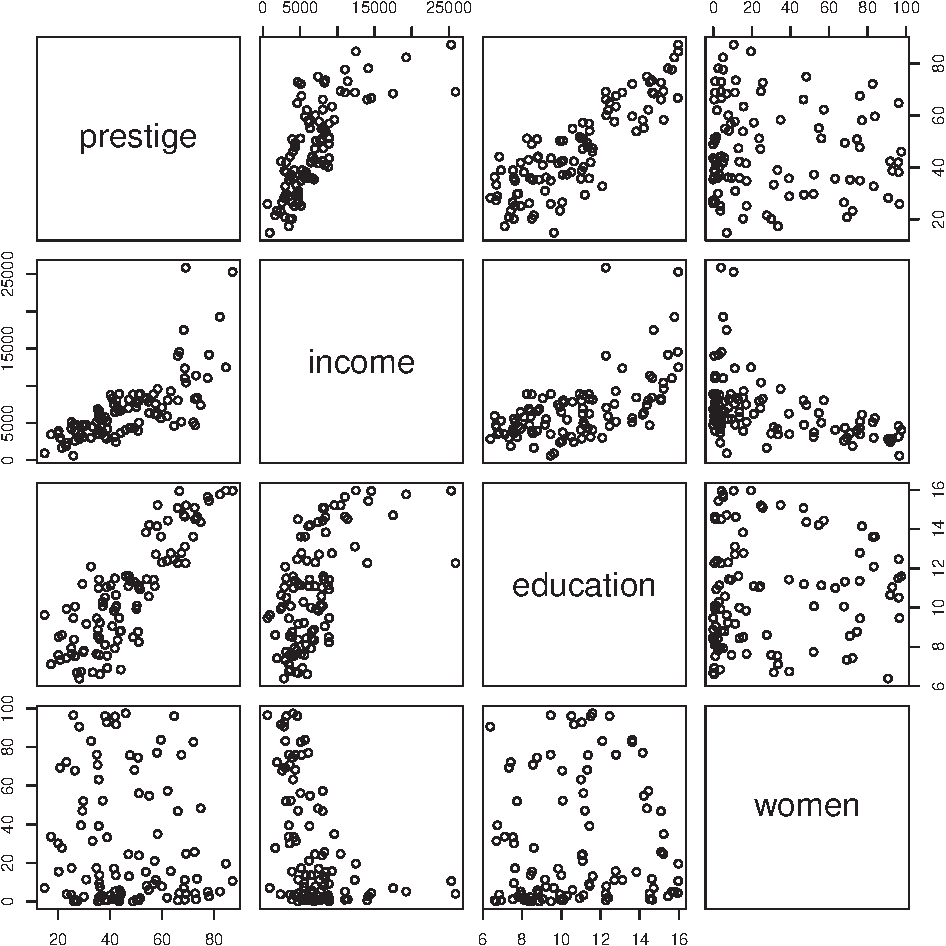
\includegraphics[width=1\textwidth,height=\textheight]{figs/ch03/fig-prestige-pairs-1.pdf}

}

\caption{\label{fig-prestige-pairs}Scatterplot matrix of the variables
in the Prestige dataset produced by \texttt{pairs()}}

\end{figure}%

The plots in the first row show what we have seen before for the
relations between prestige and income and education, adding to those the
plot of prestige vs.~\% women. Plots in the first column show the same
data, but with \(x\) and \(y\) interchanged.

But this basic \texttt{pairs()} plot is very limited. A more
feature-rich version is provided by \texttt{car::scatterplotMatrix()}
which can add the regression lines, loess smooths and data ellipses for
each pair, as shown in Figure~\ref{fig-prestige-spm1}.

The diagonal panels show density curves for the distribution of each
variable; for example, the distribution of \texttt{education} appears to
be multi-modal and that of \texttt{women} shows that most of the
occupations have a low percentage of women.

The combination of the regression line with the loess smoothed curve,
but without their confidence envelopes, provides about the right amount
of detail to take in at a glance where the relations are non-linear.
We've already seen (Figure~\ref{fig-Prestige-scatterplot-income1}) the
non-linear relation between prestige and income (row 1, column 2) when
occupational type is ignored. But all relations with income in column 2
are non-linear, reinforcing our idea (Section~\ref{sec-log-scale}) that
effects of income should be assessed on a log scale.

\begin{Shaded}
\begin{Highlighting}[]
\FunctionTok{scatterplotMatrix}\NormalTok{(}\SpecialCharTok{\textasciitilde{}}\NormalTok{ prestige }\SpecialCharTok{+}\NormalTok{ income }\SpecialCharTok{+}\NormalTok{ education }\SpecialCharTok{+}\NormalTok{ women,}
  \AttributeTok{data=}\NormalTok{Prestige,}
  \AttributeTok{regLine =} \FunctionTok{list}\NormalTok{(}\AttributeTok{method=}\NormalTok{lm, }\AttributeTok{lty=}\DecValTok{1}\NormalTok{, }\AttributeTok{lwd=}\DecValTok{2}\NormalTok{, }\AttributeTok{col=}\StringTok{"black"}\NormalTok{),}
  \AttributeTok{smooth=}\FunctionTok{list}\NormalTok{(}\AttributeTok{smoother=}\NormalTok{loessLine, }\AttributeTok{spread=}\ConstantTok{FALSE}\NormalTok{,}
              \AttributeTok{lty.smooth=}\DecValTok{1}\NormalTok{, }\AttributeTok{lwd.smooth=}\DecValTok{3}\NormalTok{, }\AttributeTok{col.smooth=}\StringTok{"red"}\NormalTok{),}
  \AttributeTok{ellipse=}\FunctionTok{list}\NormalTok{(}\AttributeTok{levels=}\FloatTok{0.68}\NormalTok{, }\AttributeTok{fill.alpha=}\FloatTok{0.1}\NormalTok{))}
\end{Highlighting}
\end{Shaded}

\begin{figure}[H]

\centering{

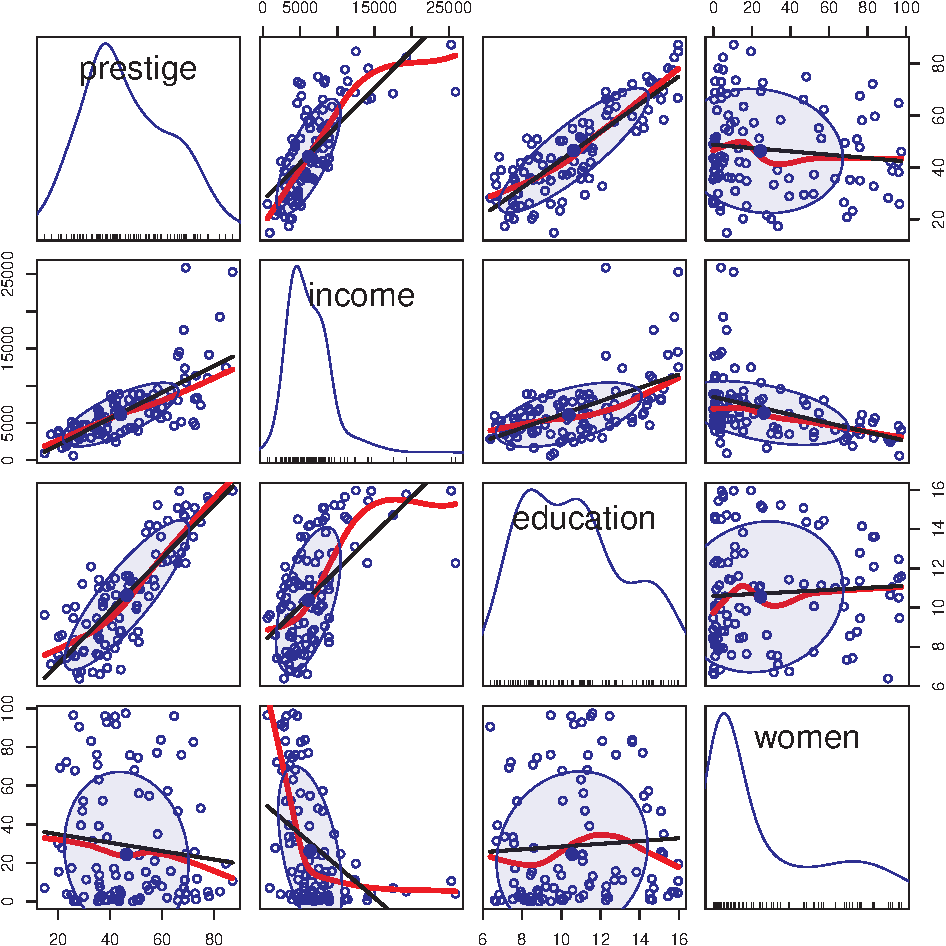
\includegraphics[width=1\textwidth,height=\textheight]{figs/ch03/fig-prestige-spm1-1.pdf}

}

\caption{\label{fig-prestige-spm1}Scatterplot matrix of the variables in
the Prestige dataset from \texttt{car::scatterplotMatrix()}.}

\end{figure}%

\texttt{scatterplotMatrix()} can also label points using the
\texttt{id\ =} argument (though this can get messy) and can stratify the
observations by a grouping variable with different symbols and colors.
For example, Figure~\ref{fig-prestige-spm2} uses the syntax
\texttt{\textasciitilde{}\ prestige\ +\ education\ +\ income\ +\ women\ \textbar{}\ type}
to provide separate regression lines, smoothed curves and data ellipses
for the three types of occupations. (The default colors are somewhat
garish, so I use \texttt{scales::hue\_pal()} to mimic the discrete color
scale used in \texttt{ggplot2}).

\begin{Shaded}
\begin{Highlighting}[]
\FunctionTok{scatterplotMatrix}\NormalTok{(}\SpecialCharTok{\textasciitilde{}}\NormalTok{ prestige }\SpecialCharTok{+}\NormalTok{ income }\SpecialCharTok{+}\NormalTok{ education }\SpecialCharTok{+}\NormalTok{ women }\SpecialCharTok{|}\NormalTok{ type,}
  \AttributeTok{data =}\NormalTok{ Prestige,}
  \AttributeTok{col =}\NormalTok{ scales}\SpecialCharTok{::}\FunctionTok{hue\_pal}\NormalTok{()(}\DecValTok{3}\NormalTok{),}
  \AttributeTok{pch =} \DecValTok{15}\SpecialCharTok{:}\DecValTok{17}\NormalTok{,}
  \AttributeTok{smooth=}\FunctionTok{list}\NormalTok{(}\AttributeTok{smoother=}\NormalTok{loessLine, }\AttributeTok{spread=}\ConstantTok{FALSE}\NormalTok{,}
              \AttributeTok{lty.smooth=}\DecValTok{1}\NormalTok{, }\AttributeTok{lwd.smooth=}\DecValTok{3}\NormalTok{, }\AttributeTok{col.smooth=}\StringTok{"black"}\NormalTok{),}
  \AttributeTok{ellipse=}\FunctionTok{list}\NormalTok{(}\AttributeTok{levels=}\FloatTok{0.68}\NormalTok{, }\AttributeTok{fill.alpha=}\FloatTok{0.1}\NormalTok{))}
\end{Highlighting}
\end{Shaded}

\begin{figure}[H]

\centering{

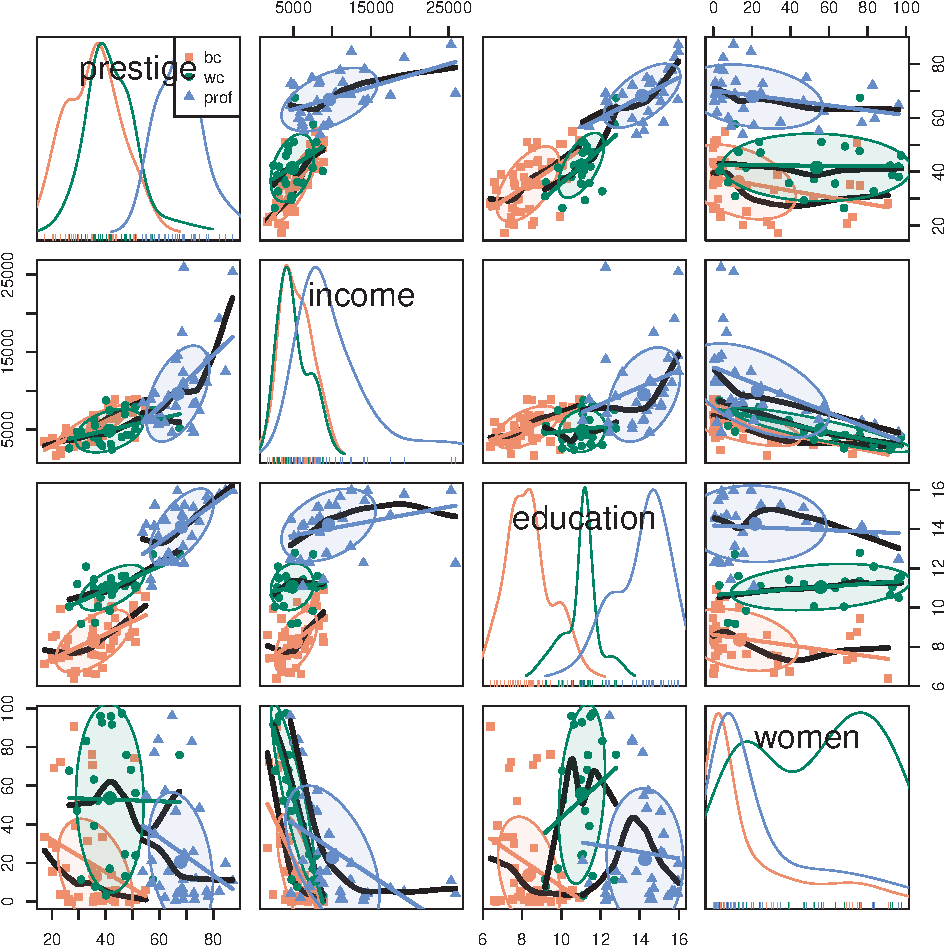
\includegraphics[width=1\textwidth,height=\textheight]{figs/ch03/fig-prestige-spm2-1.pdf}

}

\caption{\label{fig-prestige-spm2}Scatterplot matrix of the variables in
the Prestige dataset from \texttt{car::scatterplotMatrix()}, stratified
by type of occupation.}

\end{figure}%

It is now easy to see why education is multi-modal: blue collar, white
collar and professional occupations have largely non-overlapping years
of education. As well, the distribution of \% women is much higher in
the white collar category.

For the \texttt{penguins} data, given what we've seen before in
Figure~\ref{fig-peng-ggplot1} and Figure~\ref{fig-peng-ggplot2}, we may
wish to suppress details of the points (\texttt{plot.points\ =\ FALSE})
and loess smooths (\texttt{smooth\ =\ FALSE}) to focus attention on the
similarity of regression lines and data ellipses for the three penguin
species. In Figure~\ref{fig-peng-spm}, I've chosen to show boxplots
rather than density curves in the diagonal panels in order to highlight
differences in the means and interquartile ranges of the species, and to
show 68\% and 95\% data ellipses in the off-diagonal panels.

\begin{Shaded}
\begin{Highlighting}[]
\FunctionTok{scatterplotMatrix}\NormalTok{(}\SpecialCharTok{\textasciitilde{}}\NormalTok{ bill\_length }\SpecialCharTok{+}\NormalTok{ bill\_depth }\SpecialCharTok{+}\NormalTok{ flipper\_length }\SpecialCharTok{+}\NormalTok{ body\_mass }\SpecialCharTok{|}\NormalTok{ species,}
  \AttributeTok{data =}\NormalTok{ peng, }
  \AttributeTok{col =} \FunctionTok{peng.colors}\NormalTok{(}\StringTok{"medium"}\NormalTok{), }
  \AttributeTok{legend=}\ConstantTok{FALSE}\NormalTok{,}
  \AttributeTok{ellipse =} \FunctionTok{list}\NormalTok{(}\AttributeTok{levels =} \FunctionTok{c}\NormalTok{(}\FloatTok{0.68}\NormalTok{, }\FloatTok{0.95}\NormalTok{), }
                 \AttributeTok{fill.alpha =} \FloatTok{0.1}\NormalTok{),}
  \AttributeTok{regLine =} \FunctionTok{list}\NormalTok{(}\AttributeTok{lwd=}\DecValTok{3}\NormalTok{),}
  \AttributeTok{diagonal =} \FunctionTok{list}\NormalTok{(}\AttributeTok{method =} \StringTok{"boxplot"}\NormalTok{),}
  \AttributeTok{smooth =} \ConstantTok{FALSE}\NormalTok{,}
  \AttributeTok{plot.points =} \ConstantTok{FALSE}\NormalTok{,}
  \AttributeTok{cex.labels=}\DecValTok{1}\NormalTok{) }
\end{Highlighting}
\end{Shaded}

\begin{figure}[H]

\centering{

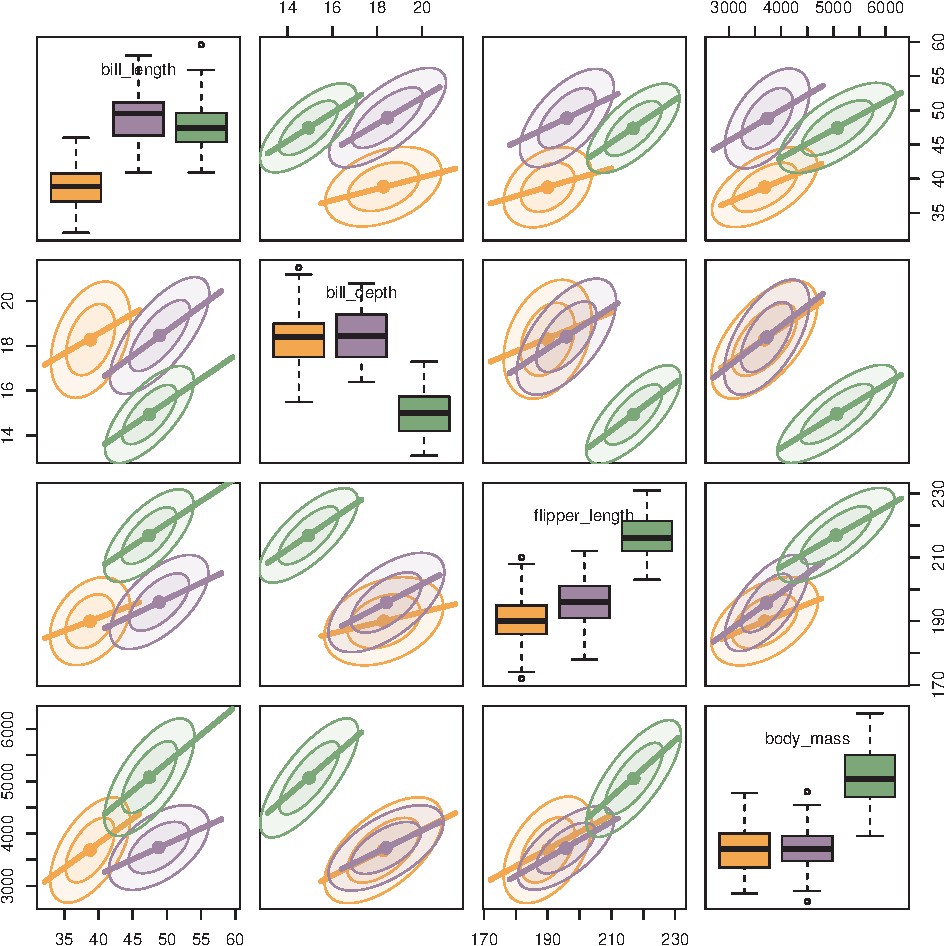
\includegraphics[width=1\textwidth,height=\textheight]{figs/ch03/fig-peng-spm-1.pdf}

}

\caption{\label{fig-peng-spm}Scatterplot matrix of the variables in the
penguins dataset, stratified by species.}

\end{figure}%

It can be seen that the species are widely separated in most of the
bivariate plots. As well, the regression lines for species have similar
slopes and the data ellipses have similar size and shape in most of the
plots. From the boxplots, we can also see that
\textcolor{orange}{Adelie} penguins have shorter bill lengths than the
others, while \textcolor{green}{Gentoo} penguins have smaller bill
depth, but longer flippers and are heavier than
\textcolor{purple}{Chinstrap} and \textcolor{orange}{Adelie} penguins.

\begin{tcolorbox}[enhanced jigsaw, breakable, left=2mm, bottomtitle=1mm, arc=.35mm, colframe=quarto-callout-note-color-frame, coltitle=black, title=\textcolor{quarto-callout-note-color}{\faInfo}\hspace{0.5em}{Looking ahead}, colback=white, toptitle=1mm, rightrule=.15mm, opacityback=0, colbacktitle=quarto-callout-note-color!10!white, titlerule=0mm, leftrule=.75mm, toprule=.15mm, bottomrule=.15mm, opacitybacktitle=0.6]

Figure~\ref{fig-peng-spm} provides a reasonably complete visual summary
of the data in relation to multivariate models that ask ``do the species
differ in their means on these body size measures?'' This corresponds to
the MANOVA model,

\begin{Shaded}
\begin{Highlighting}[]
\NormalTok{peng.mod }\OtherTok{\textless{}{-}} \FunctionTok{lm}\NormalTok{(}\FunctionTok{cbind}\NormalTok{(bill\_length, bill\_depth, flipper\_length, body\_mass) }\SpecialCharTok{\textasciitilde{}}\NormalTok{ species, }
               \AttributeTok{data=}\NormalTok{peng)}
\end{Highlighting}
\end{Shaded}

Hypothesis-error (HE) plots, described in Chapter~\ref{sec-vis-mlm}
provide a better summary of the evidence for the MANOVA test of
differences among means on all variables together. These give an
\(\mathbf{H}\) ellipse reflecting the differences among means, to be
compared with an \(\mathbf{E}\) ellipse reflecting within-group
variation and a visual test of significance.

A related question is ``how well are the penguin species distinguished
by these body size measures?'' Here, the relevant model is linear
discriminant analysis (LDA), where \texttt{species} plays the role of
the response in the model,

\begin{Shaded}
\begin{Highlighting}[]
\NormalTok{peng.lda }\OtherTok{\textless{}{-}}\NormalTok{ MASS}\SpecialCharTok{:}\FunctionTok{lda}\NormalTok{( species }\SpecialCharTok{\textasciitilde{}} \FunctionTok{cbind}\NormalTok{(bill\_length, bill\_depth, flipper\_length, body\_mass), }
               \AttributeTok{data=}\NormalTok{peng)}
\end{Highlighting}
\end{Shaded}

Both MANOVA and LDA depend on the assumption that the variances and
correlations between the variables are the same for all groups. This
assumption can be tested and visualized using the methods in
Chapter~\ref{sec-eqcov}.

\end{tcolorbox}

\subsection{Visual thinning}\label{visual-thinning}

What can you do if there are even more variables than in these examples?
If what you want is a high-level, zoomed-out display summarizing the
pairwise relations more strongly, you can apply the idea of visual
thinning to show only the most important features.

This example uses data on the rate of various crimes in the 50 U.S.
states from the United States Statistical Abstracts, 1970, used by
Hartigan (\citeproc{ref-Hartigan:75}{1975a}) and Friendly
(\citeproc{ref-Friendly:91}{1991}). These are ordered in the dataset
roughly by seriousness of crime or from crimes of violence to property
crimes.

\begin{Shaded}
\begin{Highlighting}[]
\FunctionTok{data}\NormalTok{(crime, }\AttributeTok{package =} \StringTok{"ggbiplot"}\NormalTok{)}
\FunctionTok{str}\NormalTok{(crime)}
\CommentTok{\#\textgreater{} \textquotesingle{}data.frame\textquotesingle{}:    50 obs. of  10 variables:}
\CommentTok{\#\textgreater{}  $ state   : chr  "Alabama" "Alaska" "Arizona" "Arkansas" ...}
\CommentTok{\#\textgreater{}  $ murder  : num  14.2 10.8 9.5 8.8 11.5 6.3 4.2 6 10.2 11.7 ...}
\CommentTok{\#\textgreater{}  $ rape    : num  25.2 51.6 34.2 27.6 49.4 42 16.8 24.9 39.6 31.1 ...}
\CommentTok{\#\textgreater{}  $ robbery : num  96.8 96.8 138.2 83.2 287 ...}
\CommentTok{\#\textgreater{}  $ assault : num  278 284 312 203 358 ...}
\CommentTok{\#\textgreater{}  $ burglary: num  1136 1332 2346 973 2139 ...}
\CommentTok{\#\textgreater{}  $ larceny : num  1882 3370 4467 1862 3500 ...}
\CommentTok{\#\textgreater{}  $ auto    : num  281 753 440 183 664 ...}
\CommentTok{\#\textgreater{}  $ st      : chr  "AL" "AK" "AZ" "AR" ...}
\CommentTok{\#\textgreater{}  $ region  : Factor w/ 4 levels "Northeast","South",..: 2 4 4 2 4 4 1 2 2 2 ...}
\end{Highlighting}
\end{Shaded}

Figure~\ref{fig-crime-spm} displays the scatterplot matrix for these
seven variables, using only the regression line and data ellipse to show
the linear relation and the loess smooth to show potential
non-linearity. To make this even more schematic, the axis tick marks and
labels are also removed using the \texttt{par()} settings
\texttt{xaxt\ =\ "n",\ yaxt\ =\ "n"}.

\begin{Shaded}
\begin{Highlighting}[]
\NormalTok{crime }\SpecialCharTok{|\textgreater{}}
  \FunctionTok{select}\NormalTok{(}\FunctionTok{where}\NormalTok{(is.numeric)) }\SpecialCharTok{|\textgreater{}}
  \FunctionTok{scatterplotMatrix}\NormalTok{(}
    \AttributeTok{plot.points =} \ConstantTok{FALSE}\NormalTok{,}
    \AttributeTok{ellipse =} \FunctionTok{list}\NormalTok{(}\AttributeTok{levels =} \FloatTok{0.68}\NormalTok{, }\AttributeTok{fill=}\ConstantTok{FALSE}\NormalTok{),}
    \AttributeTok{smooth =} \FunctionTok{list}\NormalTok{(}\AttributeTok{spread =} \ConstantTok{FALSE}\NormalTok{, }
                  \AttributeTok{lwd.smooth=}\DecValTok{2}\NormalTok{, }\AttributeTok{lty.smooth =} \DecValTok{1}\NormalTok{, }\AttributeTok{col.smooth =} \StringTok{"red"}\NormalTok{),}
    \AttributeTok{cex.labels =} \DecValTok{2}\NormalTok{,}
    \AttributeTok{xaxt =} \StringTok{"n"}\NormalTok{, }\AttributeTok{yaxt =} \StringTok{"n"}\NormalTok{)}
\end{Highlighting}
\end{Shaded}

\begin{figure}[H]

\centering{

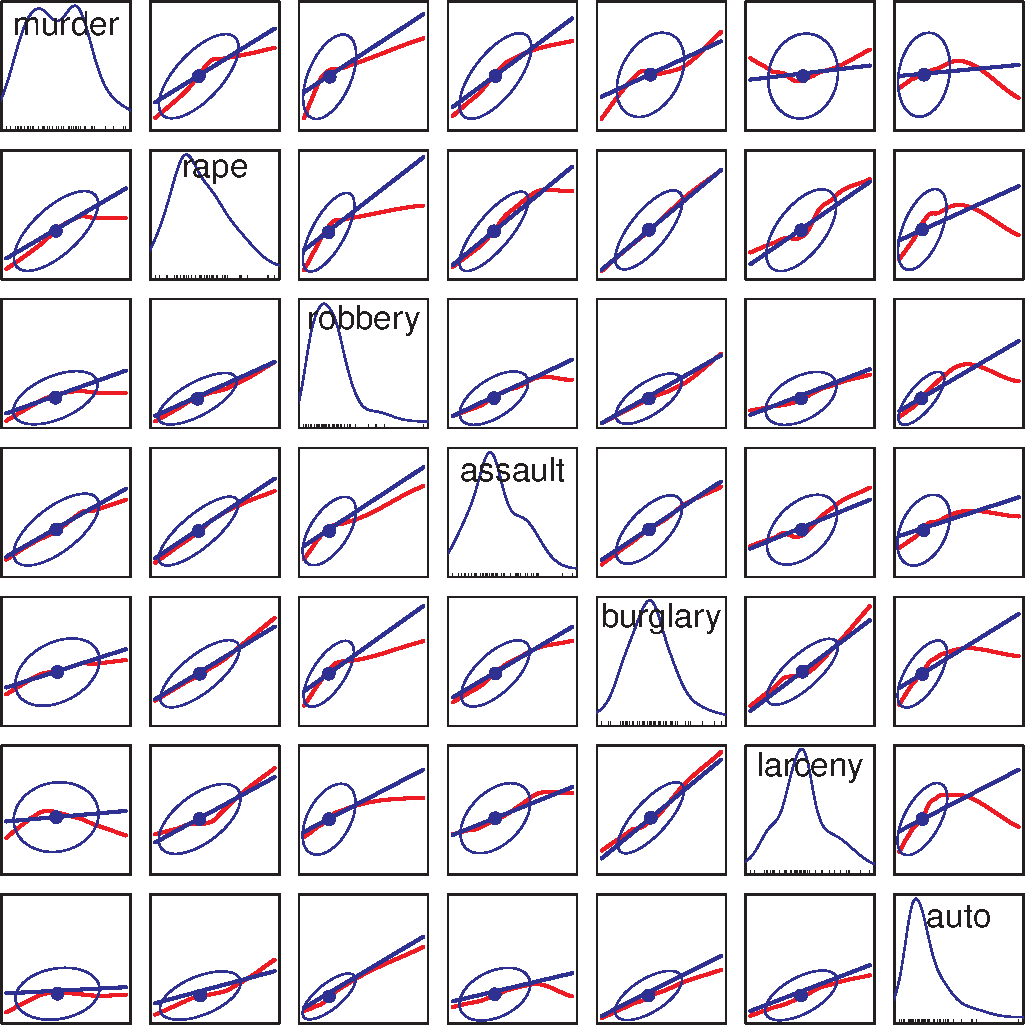
\includegraphics[width=1\textwidth,height=\textheight]{figs/ch03/fig-crime-spm-1.pdf}

}

\caption{\label{fig-crime-spm}\textbf{Visual thinning}: Scatterplot
matrix of the crime data, showing only high-level summaries of the
linear and nonlinear relations betgween each pair of variables.}

\end{figure}%

We can see that all pairwise correlations are positive, pairs closer to
the main diagonal tend to be more highly correlated and in most cases
the nonparametric smooth doesn't differ much from the linear regression
line. Exceptions to this appear mainly in the columns for
\texttt{robbery} and \texttt{auto} (auto theft).

\subsection{Corrgrams}\label{sec-corrgram}

What if you want to summarize the data even further, for example to show
only the value of the correlation for each pair of variables? A
\textbf{corrgram} (\citeproc{ref-Friendly:02:corrgram}{Friendly, 2002})
is a visual display of a correlation matrix, where the correlation can
be rendered in a variety of ways to show the direction and magnitude:
circular ``pac-man'' (or pie) symbols, ellipses, colored vars or shaded
rectangles, as shown in Figure~\ref{fig-corrgram-renderings}.

Another aspect is that of \textbf{effect ordering}
(\citeproc{ref-FriendlyKwan:03:effect}{Friendly \& Kwan, 2003}),
ordering the levels of factors and variables in graphic displays to make
important features most apparent. For variables, this means that we can
arrange the variables in a matrix-like display in such a way as to make
the pattern of relationships easiest to see. Methods to achieve this
include using principal components and cluster analysis to put the most
related variables together as described in Chapter~\ref{sec-pca-biplot}.

\begin{figure}

\centering{

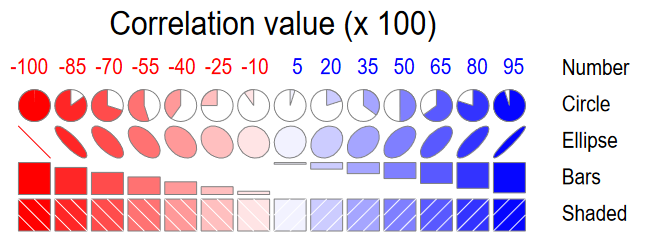
\includegraphics[width=1\textwidth,height=\textheight]{images/corrgram-renderings.png}

}

\caption{\label{fig-corrgram-renderings}\textbf{Corrgrams}: Some
renderings for the value of a correlation in a corrgram display,
conveying sign and magnitude in different ways.}

\end{figure}%

In R, these diagrams can be created using the \textbf{corrgram}
(\citeproc{ref-R-corrgram}{Wright, 2021}) and \textbf{corrplot}
(\citeproc{ref-R-corrplot}{Wei \& Simko, 2024}) packages, with different
features. \texttt{corrgram::corrgram()} is closest to Friendly
(\citeproc{ref-Friendly:02:corrgram}{2002}), in that it allows different
rendering functions for the lower, upper and diagonal panels as
illustrated in Figure~\ref{fig-corrgram-renderings}. For example, a
corrgram similar to Figure~\ref{fig-crime-spm} can be produced as
follows (not shown here):

\begin{Shaded}
\begin{Highlighting}[]
\NormalTok{crime }\SpecialCharTok{|\textgreater{}}
  \FunctionTok{select}\NormalTok{(}\FunctionTok{where}\NormalTok{(is.numeric)) }\SpecialCharTok{|\textgreater{}}
  \FunctionTok{corrgram}\NormalTok{(}\AttributeTok{lower.panel =}\NormalTok{ panel.ellipse,}
           \AttributeTok{upper.panel =}\NormalTok{ panel.ellipse,}
           \AttributeTok{diag.panel =}\NormalTok{ panel.density)}
\end{Highlighting}
\end{Shaded}

\texttt{corrplot::corrplot()} provides the rendering methods
\texttt{c("circle",\ "square",\ "ellipse",\ "number",\ "shade",\ "color",\ "pie")},
but only one can be used at a time. The function
\texttt{corrplot::corrplot.mixed()} allows different options to be
selected for the lower and upper triangles. The iconic shape is colored
with a gradient in relation to the correlation value.

\begin{Shaded}
\begin{Highlighting}[]
\NormalTok{crime }\SpecialCharTok{|\textgreater{}}
  \FunctionTok{select}\NormalTok{(}\FunctionTok{where}\NormalTok{(is.numeric)) }\SpecialCharTok{|\textgreater{}}
  \FunctionTok{cor}\NormalTok{() }\SpecialCharTok{|\textgreater{}}
  \FunctionTok{corrplot.mixed}\NormalTok{(}
           \AttributeTok{lower =} \StringTok{"ellipse"}\NormalTok{,}
           \AttributeTok{upper =} \StringTok{"pie"}\NormalTok{,}
           \AttributeTok{tl.col =} \StringTok{"black"}\NormalTok{,}
           \AttributeTok{tl.srt =} \DecValTok{0}\NormalTok{,}
           \AttributeTok{addCoef.col =} \StringTok{"black"}\NormalTok{,}
           \AttributeTok{addCoefasPercent =} \ConstantTok{TRUE}\NormalTok{)}
\end{Highlighting}
\end{Shaded}

\begin{figure}[H]

\centering{

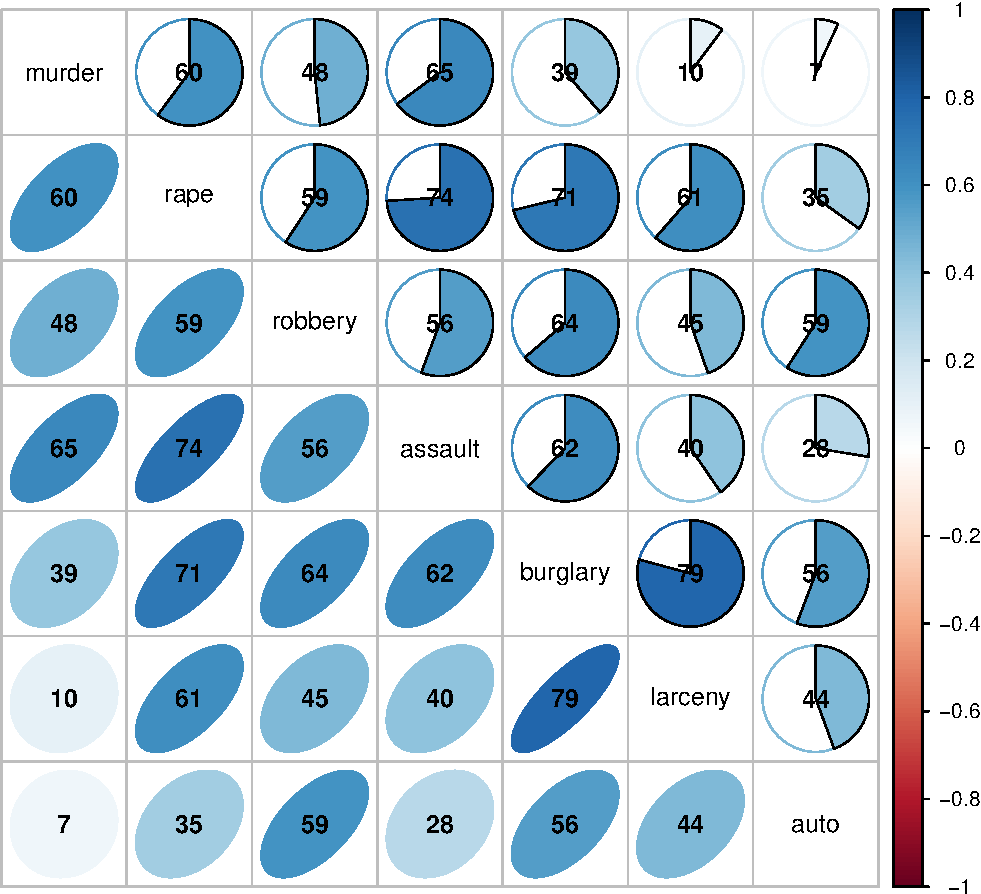
\includegraphics[width=1\textwidth,height=\textheight]{figs/ch03/fig-crime-corrplot-1.pdf}

}

\caption{\label{fig-crime-corrplot}Corrplot of the \texttt{crime} data,
showing the correlation between each pair of variables with an ellipse
(lower) and a pie chart symbol (upper), all shaded in proportion to the
correlation value, also shown numerically.}

\end{figure}%

The combination of renderings shown in Figure~\ref{fig-crime-corrplot}
is instructive. Small differences among correlation values are easier to
see with the pie symbols than with the ellipses; for example, compare
the values for murder with larceny and auto theft in row 1, columns 6-7
with those in column 1, rows 6-7, where the former are easier to
distinguish. The shading color adds another visual cue.

Variations of corrgrams are worthy replacements for a numeric table of
correlations, which are often presented in publications only for
archival value. Including the numeric value (rounded here, for
presentation purposes), makes this an attractive alternative to boring
tables of correlations.

\textbf{TODO}: Add example showing correlation ordering -- e.g.,
\texttt{mtcars} data.

\section{Generalized pairs plots}\label{sec-ggpairs}

When a dataset contains one or more discrete variables, the traditional
pairs plot cannot cope, using only color and/or point symbols to
represent categorical variables. In the context of mosaic displays and
loglinear models, representing \(n\)-way frequency tables by rectangular
tiles depicting cell frequencies, I
(\citeproc{ref-Friendly:94a}{Friendly, 1994}) proposed an analog of the
scatterplot matrix using mosaic plots for each pair of variables. The
\textbf{vcd} package (\citeproc{ref-R-vcd}{Meyer et al., 2024})
implements very general \texttt{pairs()} methods for \texttt{"table"}
objects. See my book \emph{Discrete Data Analysis with R}
(\citeproc{ref-FriendlyMeyer:2016:DDAR}{Friendly \& Meyer, 2016}) and
the \textbf{vcdExtra} (\citeproc{ref-R-vcdExtra}{\textbf{R-vcdExtra?}})
package for mosaic plots and mosaic matrices.

For example, we can tabulate the distributions of penguin species by sex
and the island where they were observed using \texttt{xtabs()}.
\texttt{ftable()} prints this three-way table more compactly. (In this
example, and what follows in the chapter, I've changed the labels for
sex from (``f'', ``m'') to (``Female'', ``Male'')).

\begin{Shaded}
\begin{Highlighting}[]
\CommentTok{\# use better labels for sex}
\NormalTok{peng }\OtherTok{\textless{}{-}}\NormalTok{ peng }\SpecialCharTok{|\textgreater{}}
  \FunctionTok{mutate}\NormalTok{(}\AttributeTok{sex =} \FunctionTok{factor}\NormalTok{(sex, }\AttributeTok{labels =} \FunctionTok{c}\NormalTok{(}\StringTok{"Female"}\NormalTok{, }\StringTok{"Male"}\NormalTok{)))}
\NormalTok{peng.table }\OtherTok{\textless{}{-}} \FunctionTok{xtabs}\NormalTok{(}\SpecialCharTok{\textasciitilde{}}\NormalTok{ species }\SpecialCharTok{+}\NormalTok{ sex }\SpecialCharTok{+}\NormalTok{ island, }\AttributeTok{data =}\NormalTok{ peng)}

\FunctionTok{ftable}\NormalTok{(peng.table)}
\CommentTok{\#\textgreater{}                  island Biscoe Dream Torgersen}
\CommentTok{\#\textgreater{} species   sex                                 }
\CommentTok{\#\textgreater{} Adelie    Female            22    27        24}
\CommentTok{\#\textgreater{}           Male              22    28        23}
\CommentTok{\#\textgreater{} Chinstrap Female             0    34         0}
\CommentTok{\#\textgreater{}           Male               0    34         0}
\CommentTok{\#\textgreater{} Gentoo    Female            58     0         0}
\CommentTok{\#\textgreater{}           Male              61     0         0}
\end{Highlighting}
\end{Shaded}

We can see immediately that the penguin species differ by island: only
Adelie were observed on all three islands; Biscoe Island had no
Chinstraps and Dream Island had no Gentoos.

\texttt{vcd::pairs()} produces all pairwise mosaic plots, as shown in
Figure~\ref{fig-peng-mosaic}. The diagonal panels show the one-way
frequencies by width of the divided bars. Each off-diagonal panel shows
the bivariate counts, breaking down each column variable by splitting
the bars in proportion to a second variable. Consequently, the frequency
of each cell is represented by its' area. The purpose is to show the
\textbf{pattern of association} between each pair, and so, the tiles in
the mosaic are shaded according to the signed standardized residual,
\(d_{ij} = (n_{ij} - \hat{n}_{ij}) / \sqrt{\hat{n}_{ij}}\) in a simple
\(\chi^2 = \Sigma_{ij} \; d_{ij}^2\) test for association---
\textcolor{blue}{blue} where the observed frequency \(n_{ij}\) is
significantly greater than expected \(\hat{n}_{ij}\) under independence,
and \textcolor{red}{red} where it is less than expected. The tiles are
unshaded when \(| d_{ij} | < 2\).

\begin{Shaded}
\begin{Highlighting}[]
\FunctionTok{library}\NormalTok{(vcd)}
\FunctionTok{pairs}\NormalTok{(peng.table, }\AttributeTok{shade =} \ConstantTok{TRUE}\NormalTok{,}
      \AttributeTok{lower\_panel\_args =} \FunctionTok{list}\NormalTok{(}\AttributeTok{labeling =} \FunctionTok{labeling\_values}\NormalTok{()),}
      \AttributeTok{upper\_panel\_args =} \FunctionTok{list}\NormalTok{(}\AttributeTok{labeling =} \FunctionTok{labeling\_values}\NormalTok{()))}
\end{Highlighting}
\end{Shaded}

\begin{figure}[H]

\centering{

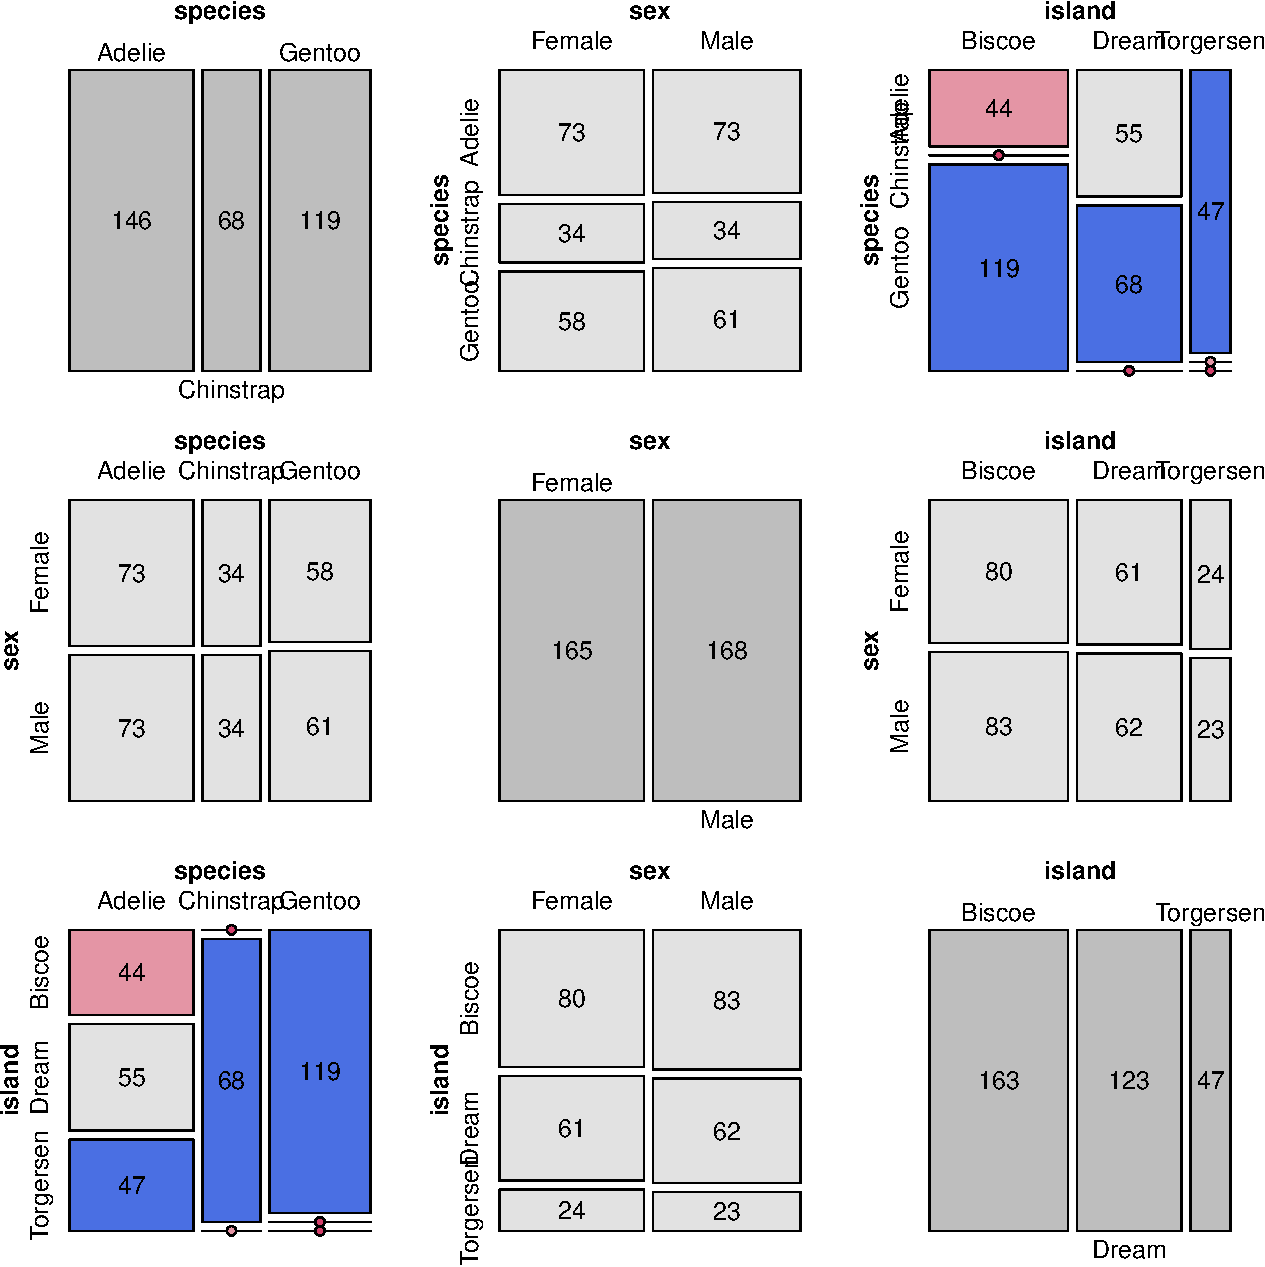
\includegraphics[width=1\textwidth,height=\textheight]{figs/ch03/fig-peng-mosaic-1.pdf}

}

\caption{\label{fig-peng-mosaic}Mosaic pairs plot for the combinations
of species, sex and island. Diagnonal plots show the marginal frequency
of each variable by the width of each rectangle. Off-diagonal mosaic
plots subdivide by the conditional frequency of the second variable,
shown numerically in the tiles.}

\end{figure}%

The shading patterns in cells (1,3) and (3,1) of
Figure~\ref{fig-peng-mosaic} show what we've seen before in the table of
frequencies: The distribution of species varies across island because on
each island one or more species did not occur. Row 2 and column 2 show
that sex is nearly exactly proportional among species and islands,
indicating independence,
\(\text{sex} \perp \{\text{species}, \text{island}\}\). More
importantly, mosaic pairs plots can show, at a glance, all (bivariate)
associations among multivariate categorical variables.

The next step, by John Emerson and others
(\citeproc{ref-Emerson-etal:2013}{Emerson et al., 2013}) was to
recognize that combinations of continuous and discrete, categorical
variables could be plotted in different ways.

\begin{itemize}
\tightlist
\item
  Two continuous variables can be shown as a standard scatterplot of
  points and/or bivariate density contours, or simply by numeric
  summaries such as a correlation value;
\item
  A pair of one continuous and one categorical variable can be shown as
  side-by-side boxplots or violin plots, histograms or density plots;
\item
  Two categorical variables could be shown in a mosaic plot or by
  grouped bar plots.
\end{itemize}

In the \textbf{ggplot2} framework, these displays are implemented using
the \texttt{ggpairs()} function from the \textbf{GGally} package
(\citeproc{ref-R-GGally}{Schloerke et al., 2024}). This allows different
plot types to be shown in the lower and upper triangles and in the
diagonal cells of the plot matrix. As well, aesthetics such as color and
shape can be used within the plots to distinguish groups directly. As
illustrated below, you can define custom functions to control exactly
what is plotted in any panel.

The basic, default plot shows scatterplots for pairs of continuous
variables in the lower triangle and the values of correlations in the
upper triangle. A combination of a discrete and continuous variables is
plotted as histograms in the lower triangle and boxplots in the upper
triangle. Figure~\ref{fig-peng-ggpairs1} includes \texttt{sex} to
illustrate the combinations.

\begin{Shaded}
\begin{Highlighting}[]
\FunctionTok{ggpairs}\NormalTok{(peng, }\AttributeTok{columns=}\FunctionTok{c}\NormalTok{(}\DecValTok{3}\SpecialCharTok{:}\DecValTok{6}\NormalTok{, }\DecValTok{7}\NormalTok{),}
        \FunctionTok{aes}\NormalTok{(}\AttributeTok{color=}\NormalTok{species, }\AttributeTok{alpha=}\FloatTok{0.5}\NormalTok{),}
        \AttributeTok{progress =} \ConstantTok{FALSE}\NormalTok{) }\SpecialCharTok{+}
  \FunctionTok{theme\_penguins}\NormalTok{() }\SpecialCharTok{+}
  \FunctionTok{theme}\NormalTok{(}\AttributeTok{axis.text.x =} \FunctionTok{element\_text}\NormalTok{(}\AttributeTok{angle =} \SpecialCharTok{{-}}\DecValTok{45}\NormalTok{))}
\end{Highlighting}
\end{Shaded}

\begin{figure}[H]

\centering{

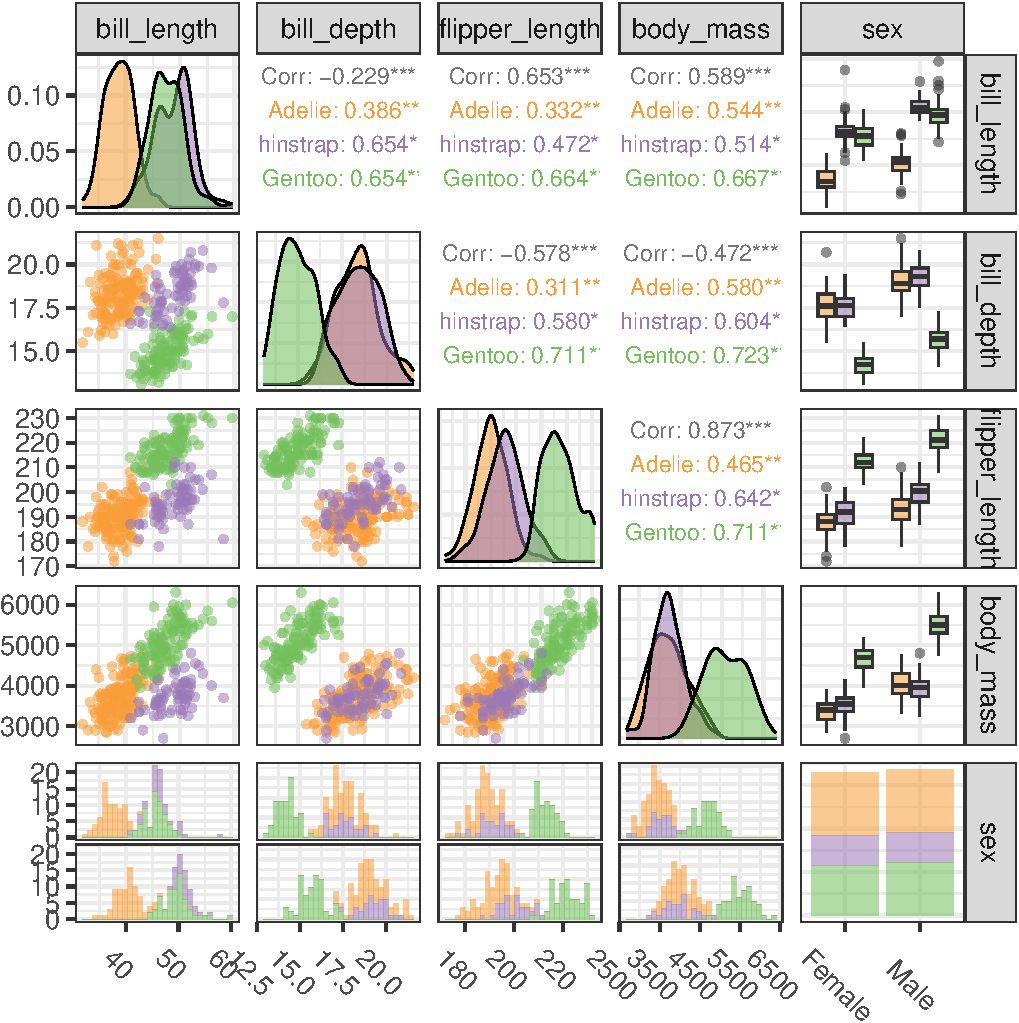
\includegraphics[width=1\textwidth,height=\textheight]{figs/ch03/fig-peng-ggpairs1-1.pdf}

}

\caption{\label{fig-peng-ggpairs1}Basic \texttt{ggpairs()} plot of
penguin size variables and sex, stratified by species.}

\end{figure}%

To my eye, printing the values of correlations in the upper triangle is
often a waste of graphic space. But this example shows something
peculiar and interesting if you look closely: In all pairs among the
penguin size measurements, there are positive correlations within each
species, as we can see in Figure~\ref{fig-peng-spm}. Yet, in three of
these panels, the overall correlation ignoring species is negative. For
example, the overall correlation between bill depth and flipper length
is \(r = -0.579\) in row 2, column 3; the scatterplot in the diagonally
opposite cell, row 3, column 2 shows the data. These cases, of differing
signs for an overall correlation, ignoring a group variable and the
within group correlations are examples of \textbf{Simpson's Paradox},
explored later in Chapter XX.

The last row and column, for \texttt{sex} in
Figure~\ref{fig-peng-ggpairs1}, provides an initial glance at the issue
of sex differences among penguin species that motivated the collection
of these data. We can go further by also examining differences among
species and island, but first we need to understand how to display
exactly what we want for each pairwise plot.

\texttt{ggpairs()} is extremely general in that for each of the
\texttt{lower}, \texttt{upper} and \texttt{diag} sections you can assign
any of a large number of built-in functions (of the form
\texttt{ggally\_NAME}), or your own custom function for what is plotted,
depending on the types of variables in each plot.

\begin{itemize}
\tightlist
\item
  \texttt{continuous}: both X and Y are continuous variables, supply
  this as the \texttt{NAME} part of a \texttt{ggally\_NAME()} function
  or the name of a custom function;
\item
  \texttt{combo}: one X of and Y variable is discrete while the other is
  continuous, using the same convention;
\item
  \texttt{discrete}: both X and Y are discrete variables.
\end{itemize}

The defaults, which were used in Figure~\ref{fig-peng-ggpairs1}, are:

\begin{Shaded}
\begin{Highlighting}[]
\NormalTok{upper }\OtherTok{=} \FunctionTok{list}\NormalTok{(}\AttributeTok{continuous =} \StringTok{"cor"}\NormalTok{,          }\CommentTok{\# correlation values}
             \AttributeTok{combo =} \StringTok{"box\_no\_facet"}\NormalTok{,      }\CommentTok{\# boxplots }
             \AttributeTok{discrete =} \StringTok{"count"}\NormalTok{)          }\CommentTok{\# rectangles \textasciitilde{} count}
\NormalTok{lower }\OtherTok{=} \FunctionTok{list}\NormalTok{(}\AttributeTok{continuous =} \StringTok{"points"}\NormalTok{,       }\CommentTok{\# just data points}
             \AttributeTok{combo =} \StringTok{"facethist"}\NormalTok{,         }\CommentTok{\# faceted histograms}
             \AttributeTok{discrete =} \StringTok{"facetbar"}\NormalTok{)       }\CommentTok{\# faceted bar plots}
\NormalTok{diag  }\OtherTok{=} \FunctionTok{list}\NormalTok{(}\AttributeTok{continuous =} \StringTok{"densityDiag"}\NormalTok{,  }\CommentTok{\# density plots}
             \AttributeTok{discrete =} \StringTok{"barDiag"}\NormalTok{)        }\CommentTok{\# bar plots}
\end{Highlighting}
\end{Shaded}

Thus, \texttt{ggpairs()} uses \texttt{ggally\_cor()} to print the
correlation values for pairs of continuous variables in the upper
triangle, and uses \texttt{ggally\_points()} to plot scatterplots of
points in the lower portion. The diagonal panels as shown as density
plots (\texttt{ggally\_densityDiag()}) for continuous variables but as
bar plots (\texttt{ggally\_barDiag()}) for discrete factors.

See the vignette,
\href{https://ggobi.github.io/ggally/articles/ggally_plots.html}{ggally\_plots}
for an illustrated list of available high-level plots. For our purpose
here, which is to illustrate enhanced displays, note that for
scatterplots of continuous variables, there are two functions which plot
the points and also add a smoother, \texttt{\_lm} or \texttt{\_loess}.

\begin{Shaded}
\begin{Highlighting}[]
\FunctionTok{ls}\NormalTok{(}\FunctionTok{getNamespace}\NormalTok{(}\StringTok{"GGally"}\NormalTok{)) }\SpecialCharTok{|\textgreater{}} 
\NormalTok{  stringr}\SpecialCharTok{::}\FunctionTok{str\_subset}\NormalTok{(}\StringTok{"\^{}ggally\_smooth\_"}\NormalTok{)}
\CommentTok{\#\textgreater{} [1] "ggally\_smooth\_lm"    "ggally\_smooth\_loess"}
\end{Highlighting}
\end{Shaded}

A customized display for scatterplots of continuous variables can be any
function that takes \texttt{data} and \texttt{mapping} arguments and
returns a \texttt{"ggplot"} object. The \texttt{mapping} argument
supplies the aesthetics, e.g., \texttt{aes(color=species,\ alpha=0.5)},
but only if you wish to override what is supplied in the
\texttt{ggpairs()} call.

Here is a function, \texttt{my\_panel()} that plots the data points,
regression line and loess smooth:

\begin{Shaded}
\begin{Highlighting}[]
\NormalTok{my\_panel }\OtherTok{\textless{}{-}} \ControlFlowTok{function}\NormalTok{(data, mapping, ...)\{}
\NormalTok{  p }\OtherTok{\textless{}{-}} \FunctionTok{ggplot}\NormalTok{(}\AttributeTok{data =}\NormalTok{ data, }\AttributeTok{mapping =}\NormalTok{ mapping) }\SpecialCharTok{+} 
    \FunctionTok{geom\_point}\NormalTok{() }\SpecialCharTok{+} 
    \FunctionTok{geom\_smooth}\NormalTok{(}\AttributeTok{method=}\NormalTok{lm, }\AttributeTok{formula =}\NormalTok{ y }\SpecialCharTok{\textasciitilde{}}\NormalTok{ x, }\AttributeTok{se =} \ConstantTok{FALSE}\NormalTok{, ...) }\SpecialCharTok{+}
    \FunctionTok{geom\_smooth}\NormalTok{(}\AttributeTok{method=}\NormalTok{loess, }\AttributeTok{formula =}\NormalTok{ y }\SpecialCharTok{\textasciitilde{}}\NormalTok{ x, }\AttributeTok{se =} \ConstantTok{FALSE}\NormalTok{, ...)}
\NormalTok{  p}
\NormalTok{\}}
\end{Highlighting}
\end{Shaded}

For this example, I want only simple summaries of for the scatterplots,
so I don't want to plot the data points, but do want to add the
regression line and a data ellipse.

\begin{Shaded}
\begin{Highlighting}[]
\NormalTok{my\_panel1 }\OtherTok{\textless{}{-}} \ControlFlowTok{function}\NormalTok{(data, mapping, ...)\{}
\NormalTok{  p }\OtherTok{\textless{}{-}} \FunctionTok{ggplot}\NormalTok{(}\AttributeTok{data =}\NormalTok{ data, }\AttributeTok{mapping =}\NormalTok{ mapping) }\SpecialCharTok{+} 
     \FunctionTok{geom\_smooth}\NormalTok{(}\AttributeTok{method=}\NormalTok{lm, }\AttributeTok{formula =}\NormalTok{ y }\SpecialCharTok{\textasciitilde{}}\NormalTok{ x, }\AttributeTok{se =} \ConstantTok{FALSE}\NormalTok{, ...) }\SpecialCharTok{+}
     \FunctionTok{stat\_ellipse}\NormalTok{(}\AttributeTok{geom =} \StringTok{"polygon"}\NormalTok{, }\AttributeTok{level =} \FloatTok{0.68}\NormalTok{, ...)}
\NormalTok{  p}
\NormalTok{\}}
\end{Highlighting}
\end{Shaded}

Then, to show what can be done, Figure~\ref{fig-peng-ggpairs7} uses
\texttt{my\_panel1()} for the scatterplots in the 4 x 4 block of plots
in the upper left. The combination of the continuous body size measures
and the discrete factors \texttt{species}, \texttt{island} and
\texttt{sex} are shown in upper triangle by boxplots but by faceted
histograms in the lower portion. The factors are shown as rectangles
with area proportional to count (poor-man's mosaic plots) above the
diagonal and as faceted bar plots below.

\begin{Shaded}
\begin{Highlighting}[]
\FunctionTok{ggpairs}\NormalTok{(peng, }\AttributeTok{columns=}\FunctionTok{c}\NormalTok{(}\DecValTok{3}\SpecialCharTok{:}\DecValTok{6}\NormalTok{, }\DecValTok{1}\NormalTok{, }\DecValTok{2}\NormalTok{, }\DecValTok{7}\NormalTok{),}
        \AttributeTok{mapping =} \FunctionTok{aes}\NormalTok{(}\AttributeTok{color=}\NormalTok{species, }\AttributeTok{fill =}\NormalTok{ species, }\AttributeTok{alpha=}\FloatTok{0.2}\NormalTok{),}
        \AttributeTok{lower =} \FunctionTok{list}\NormalTok{(}\AttributeTok{continuous =}\NormalTok{ my\_panel1),}
        \AttributeTok{upper =} \FunctionTok{list}\NormalTok{(}\AttributeTok{continuous =}\NormalTok{ my\_panel1),}
        \AttributeTok{progress =} \ConstantTok{FALSE}\NormalTok{) }\SpecialCharTok{+}
  \FunctionTok{theme\_penguins}\NormalTok{() }\SpecialCharTok{+}
  \FunctionTok{theme}\NormalTok{(}\AttributeTok{panel.grid.major =} \FunctionTok{element\_blank}\NormalTok{(), }
        \AttributeTok{panel.grid.minor =} \FunctionTok{element\_blank}\NormalTok{()) }\SpecialCharTok{+} 
  \FunctionTok{theme}\NormalTok{(}\AttributeTok{axis.text.x =} \FunctionTok{element\_text}\NormalTok{(}\AttributeTok{angle =} \SpecialCharTok{{-}}\DecValTok{45}\NormalTok{))}
\end{Highlighting}
\end{Shaded}

\begin{figure}[H]

\centering{

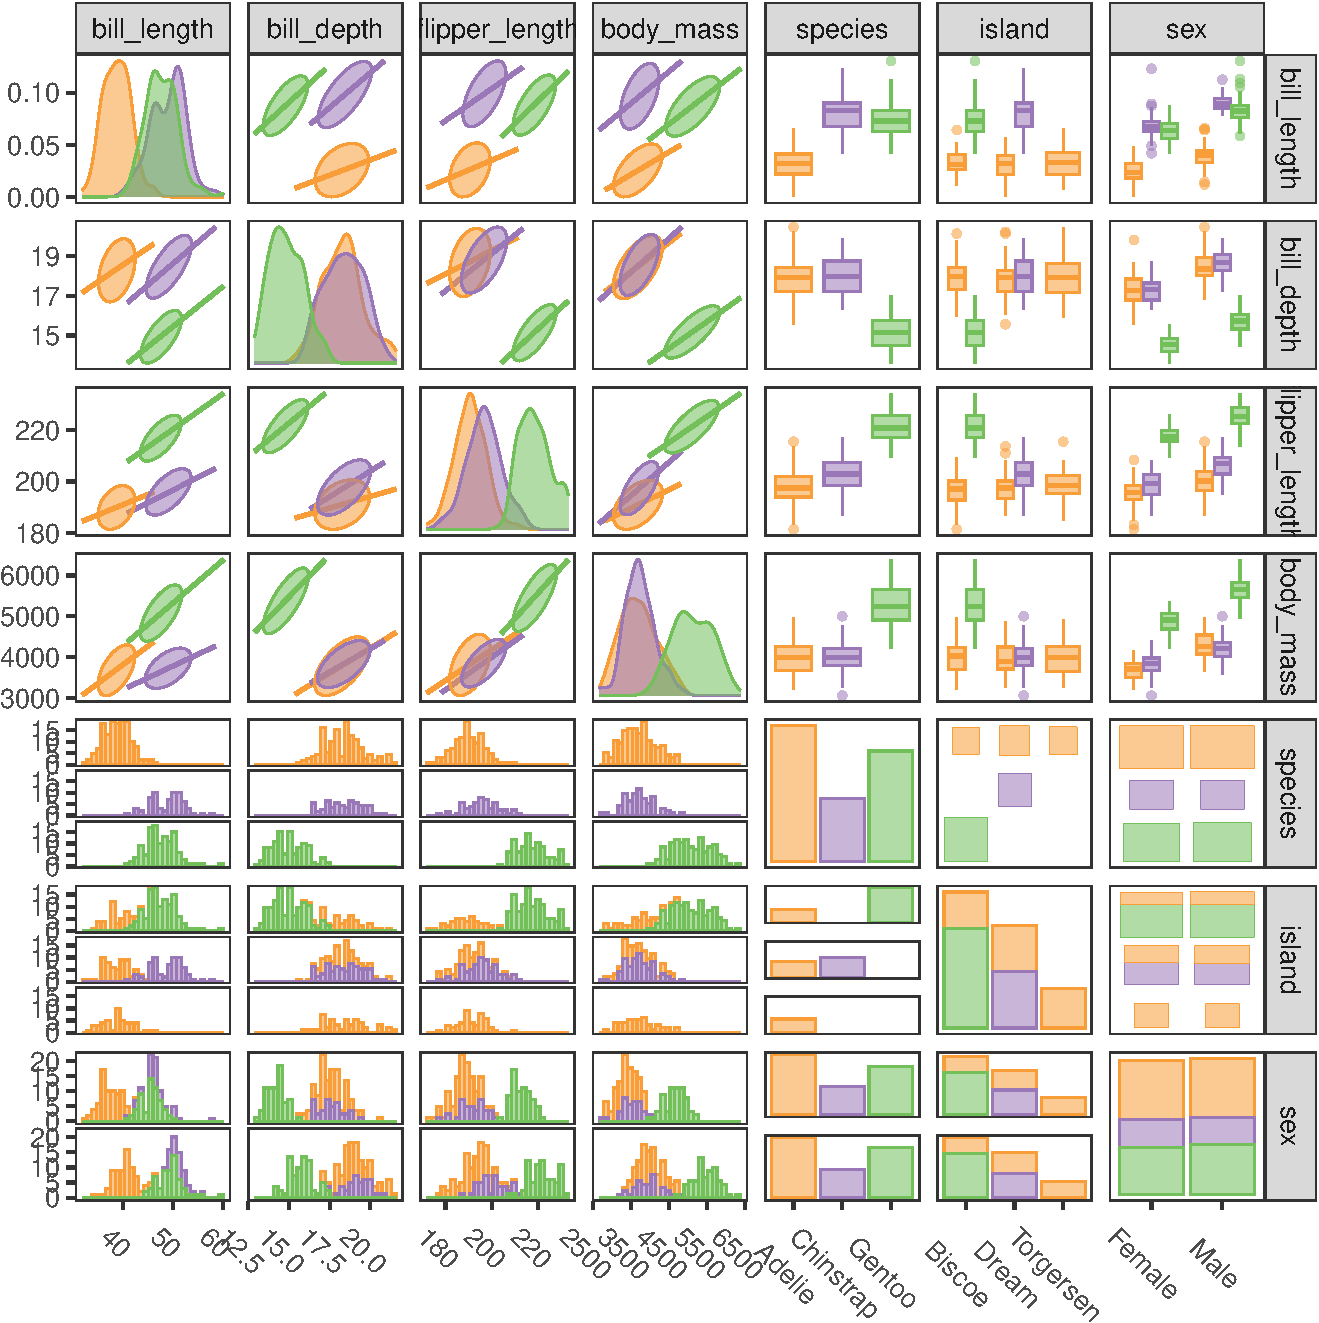
\includegraphics[width=1\textwidth,height=\textheight]{figs/ch03/fig-peng-ggpairs7-1.pdf}

}

\caption{\label{fig-peng-ggpairs7}Customized \texttt{ggpairs()} plot of
penguin size variables, together with species, island and sex.}

\end{figure}%

There is certainly a lot going on in Figure~\ref{fig-peng-ggpairs7}, but
it does show a high-level overview of all the variables (except
\texttt{year}) in the penguins dataset.

\section{Parallel coordinate plots}\label{sec-parcoord}

As we have seen above, scatterplot matrices and generalized pairs plots
extend data visualization to multivariate data, but these variables
share one 2D space, so resolution decreases as the number of variable
increase. You need a very large screen or sheet of paper to see more
than, say 5-6 variables with any clarity.

Parallel coordinate plots are an attractive alternative, with which we
can visualize an arbitrary number of variables to get a visual summary
of a potentially high-dimensional dataset, and perhaps recognize
outliers and clusters in the data in a different way. In these plots,
each variable is shown on a separate, parallel axis. A multivariate
observation is then plotted by connecting their respective values on
each axis with lines across all the axes.

The geometry of parallel coordinates is interesting, because what is a
point in \(n\)-dimensional (Euclidean) \emph{data} space becomes a line
in the \emph{projective} parallel coordinate space with \(n\) axes, and
vice-versa: lines in parallel coordinate space correspond to points in
data space. Thus, a collection of points in data space map to lines that
intersect in a point in projective space. What this does is to map
\(n\)-dimensional relations into 2D patterns we can see in a parallel
coordinates plot.

\begin{tcolorbox}[enhanced jigsaw, breakable, left=2mm, bottomtitle=1mm, arc=.35mm, colframe=quarto-callout-note-color-frame, coltitle=black, title=\textcolor{quarto-callout-note-color}{\faInfo}\hspace{0.5em}{History Corner}, colback=white, toptitle=1mm, rightrule=.15mm, opacityback=0, colbacktitle=quarto-callout-note-color!10!white, titlerule=0mm, leftrule=.75mm, toprule=.15mm, bottomrule=.15mm, opacitybacktitle=0.6]

\begin{quote}
Those who don't know history are doomed to plagarize it ---The author
\end{quote}

The theory of projective geometry originated with the French
mathematician Maurice d'Ocagne (\citeproc{ref-Ocagne:1885}{1885}) who
sought a way to provide graphic calculation of mathematical functions
with alignment diagrams or \emph{nomograms} using parallel axes with
different scales. A three-variable equation, for example, could be
solved using three parallel axes, where known values could be marked on
their scales, a line drawn between them, and an unknown read on its
scale at the point where the line intersects that scale.

Henry Gannet (1880), in work preceding the \emph{Statistical Atlas of
the United States} for the 1890 Census
(\citeproc{ref-Gannett:1898}{Gannett, 1898}), is widely credited with
being the first to use parallel coordinates plots to show data, in his
case, to show the
\href{https://www.davidrumsey.com/luna/servlet/detail/RUMSEY~8~1~32803~1152181}{rank
ordering of US states} by 10 measures including population, occupations,
wealth, manufacturing, agriculture and so on.

However, both d'Ocagne and Gannet were far preceded in this by
Andre-Michel Guerry (\citeproc{ref-Guerry:1833}{1833}) who used this
method to show how the rank order of various crimes changed with age of
the accused. See Friendly (\citeproc{ref-Friendly2022}{2022}), Figure 7
for his version and for an appreciation of the remarkable contributions
of this amateur statistician to the history of data visualization.

The use of parallel coordinates for display of multidimensional data was
rediscovered by Alfred Inselberg (\citeproc{ref-Inselberg:1985}{1985})
and extended by Edward Wegman (\citeproc{ref-Wegman:1990}{1990}),
neither of whom recognized the earlier history. Somewhat earlier, David
Andrews (\citeproc{ref-Andrews:72}{1972}) proposed mapping multivariate
observations to smooth Fourrier functions composed of alternating
\(\sin()\) and \(\cos()\) terms. And in my book, \emph{SAS System for
Statistical Graphics} (\citeproc{ref-Friendly:91}{Friendly, 1991}), I
implemented what I called
\href{https://blogs.sas.com/content/iml/2022/11/14/profile-plots-sas.html}{\emph{profile
plots}} without knowing their earlier history as parallel coordinate
plots.

\end{tcolorbox}

Parallel coordinate plots present a challenge for graphic developers, in
that they require a different way to think about plot construction for
multiple variables, which can be quantitative, as in the original idea,
or categorical factors, all to be shown along parallel axes.

Here, I use the \textbf{ggpcp} package (\citeproc{ref-R-ggpcp}{Hofmann
et al., 2022}), best described in VanderPlas et al.
(\citeproc{ref-VanderPlas2023}{2023}), who also review the modern
history. This takes some getting used to, because they develop
\texttt{pcp\_*()} extensions of the \texttt{ggplot2} grammar of graphics
framework to allow:

\begin{itemize}
\tightlist
\item
  \texttt{pcp\_select()}: selections of the variables to be plotted and
  their horizontal order on parallel axes,
\item
  \texttt{pcp\_scale()}: methods for scaling of the variables to each
  axis,
\item
  \texttt{pcp\_arrange()}: methods for breaking ties in factor variables
  to space them out.
\end{itemize}

Then, it provides \texttt{geom\_pcp\_*()} functions to control the
display of axes with appropriate aesthetics, labels for categorical
factors and so forth. \textbf{?@fig-peng-ggpcp1} illustrates this type
of display, using sex and species in addition to the quantitative
variables for the penguin data.

\begin{Shaded}
\begin{Highlighting}[]
\NormalTok{peng }\SpecialCharTok{|\textgreater{}}
  \FunctionTok{pcp\_select}\NormalTok{(bill\_length}\SpecialCharTok{:}\NormalTok{body\_mass, sex, species) }\SpecialCharTok{|\textgreater{}}
  \FunctionTok{pcp\_scale}\NormalTok{(}\AttributeTok{method =} \StringTok{"uniminmax"}\NormalTok{) }\SpecialCharTok{|\textgreater{}}
  \FunctionTok{pcp\_arrange}\NormalTok{() }\SpecialCharTok{|\textgreater{}}
  \FunctionTok{ggplot}\NormalTok{(}\FunctionTok{aes\_pcp}\NormalTok{()) }\SpecialCharTok{+}
  \FunctionTok{geom\_pcp\_axes}\NormalTok{() }\SpecialCharTok{+}
  \FunctionTok{geom\_pcp}\NormalTok{(}\FunctionTok{aes}\NormalTok{(}\AttributeTok{colour =}\NormalTok{ species), }\AttributeTok{alpha =} \FloatTok{0.8}\NormalTok{, }\AttributeTok{overplot =} \StringTok{"none"}\NormalTok{) }\SpecialCharTok{+}
  \FunctionTok{geom\_pcp\_labels}\NormalTok{() }\SpecialCharTok{+}
  \FunctionTok{scale\_colour\_manual}\NormalTok{(}\AttributeTok{values =} \FunctionTok{peng.colors}\NormalTok{()) }\SpecialCharTok{+}
  \FunctionTok{labs}\NormalTok{(}\AttributeTok{x =} \StringTok{""}\NormalTok{, }\AttributeTok{y =} \StringTok{""}\NormalTok{) }\SpecialCharTok{+}
  \FunctionTok{theme}\NormalTok{(}\AttributeTok{axis.title.y =} \FunctionTok{element\_blank}\NormalTok{(), }\AttributeTok{axis.text.y =} \FunctionTok{element\_blank}\NormalTok{(), }
        \AttributeTok{axis.ticks.y =} \FunctionTok{element\_blank}\NormalTok{(), }\AttributeTok{legend.position =} \StringTok{"none"}\NormalTok{)}
\end{Highlighting}
\end{Shaded}

\begin{center}
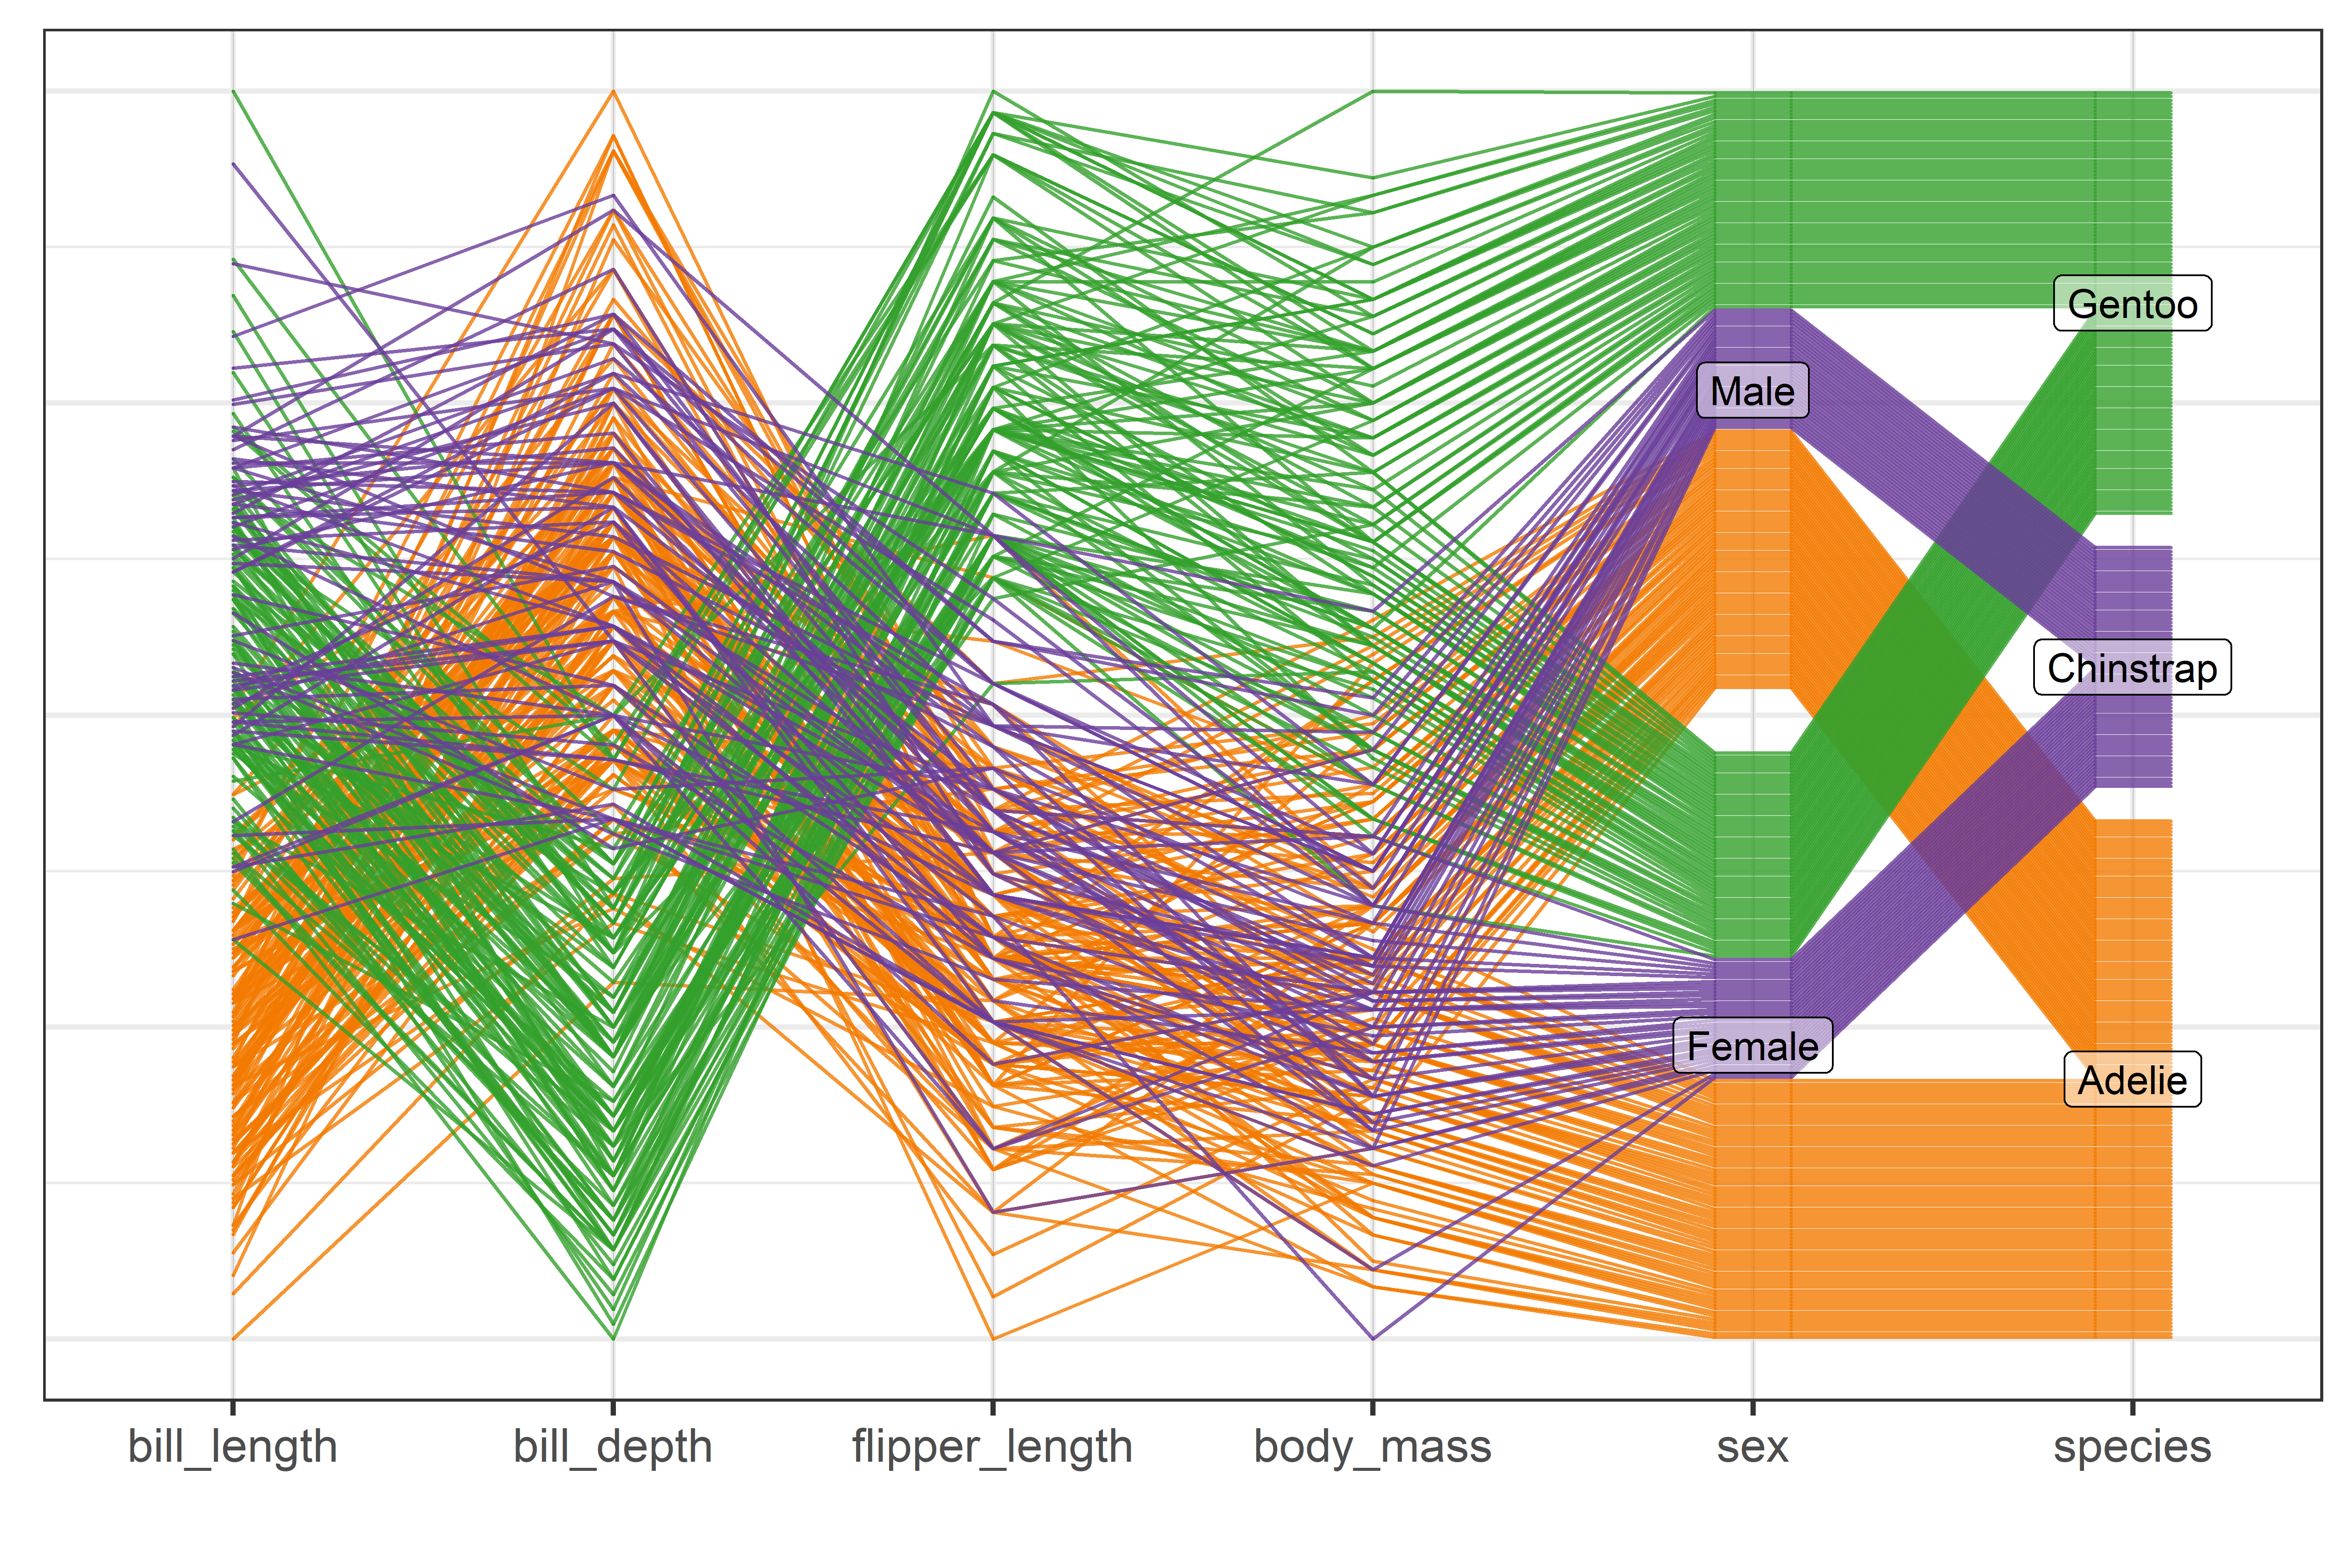
\includegraphics[width=18in,height=\textheight]{figs/fig-peng-ggpcp1-1.png}
\end{center}

Rearranging the order of variables and the ordering of factor levels can
make a difference in what we can see in such plots. For a simple example
(following VanderPlas et al. (\citeproc{ref-VanderPlas2023}{2023})), we
reorder the levels of species and islands to make it clearer which
species occur on each island.

\begin{Shaded}
\begin{Highlighting}[]
\NormalTok{peng1 }\OtherTok{\textless{}{-}}\NormalTok{ peng }\SpecialCharTok{|\textgreater{}}
  \FunctionTok{mutate}\NormalTok{(}\AttributeTok{species =} \FunctionTok{factor}\NormalTok{(species, }\AttributeTok{levels =} \FunctionTok{c}\NormalTok{(}\StringTok{"Chinstrap"}\NormalTok{, }\StringTok{"Adelie"}\NormalTok{, }\StringTok{"Gentoo"}\NormalTok{))) }\SpecialCharTok{|\textgreater{}}
  \FunctionTok{mutate}\NormalTok{(}\AttributeTok{island =} \FunctionTok{factor}\NormalTok{(island, }\AttributeTok{levels =} \FunctionTok{c}\NormalTok{(}\StringTok{"Dream"}\NormalTok{, }\StringTok{"Torgersen"}\NormalTok{, }\StringTok{"Biscoe"}\NormalTok{)))}

\NormalTok{peng1 }\SpecialCharTok{|\textgreater{}}
  \FunctionTok{pcp\_select}\NormalTok{(species, island, bill\_length}\SpecialCharTok{:}\NormalTok{body\_mass) }\SpecialCharTok{|\textgreater{}}
  \FunctionTok{pcp\_scale}\NormalTok{() }\SpecialCharTok{|\textgreater{}}
  \FunctionTok{pcp\_arrange}\NormalTok{(}\AttributeTok{method =} \StringTok{"from{-}left"}\NormalTok{) }\SpecialCharTok{|\textgreater{}}
  \FunctionTok{ggplot}\NormalTok{(}\FunctionTok{aes\_pcp}\NormalTok{()) }\SpecialCharTok{+}
  \FunctionTok{geom\_pcp\_axes}\NormalTok{() }\SpecialCharTok{+}
  \FunctionTok{geom\_pcp}\NormalTok{(}\FunctionTok{aes}\NormalTok{(}\AttributeTok{colour =}\NormalTok{ species), }\AttributeTok{alpha =} \FloatTok{0.6}\NormalTok{, }\AttributeTok{overplot =} \StringTok{"none"}\NormalTok{) }\SpecialCharTok{+}
  \FunctionTok{geom\_pcp\_boxes}\NormalTok{(}\AttributeTok{fill =} \StringTok{"white"}\NormalTok{, }\AttributeTok{alpha =} \FloatTok{0.5}\NormalTok{) }\SpecialCharTok{+}
  \FunctionTok{geom\_pcp\_labels}\NormalTok{() }\SpecialCharTok{+}
  \FunctionTok{scale\_colour\_manual}\NormalTok{(}\AttributeTok{values =} \FunctionTok{peng.colors}\NormalTok{()[}\FunctionTok{c}\NormalTok{(}\DecValTok{2}\NormalTok{,}\DecValTok{1}\NormalTok{,}\DecValTok{3}\NormalTok{)]) }\SpecialCharTok{+}
  \FunctionTok{theme\_bw}\NormalTok{() }\SpecialCharTok{+}
  \FunctionTok{labs}\NormalTok{(}\AttributeTok{x =} \StringTok{""}\NormalTok{, }\AttributeTok{y =} \StringTok{""}\NormalTok{) }\SpecialCharTok{+}
  \FunctionTok{theme}\NormalTok{(}\AttributeTok{axis.text.y =} \FunctionTok{element\_blank}\NormalTok{(), }\AttributeTok{axis.ticks.y =} \FunctionTok{element\_blank}\NormalTok{(),}
        \AttributeTok{legend.position =} \StringTok{"none"}\NormalTok{) }
\end{Highlighting}
\end{Shaded}

\begin{center}
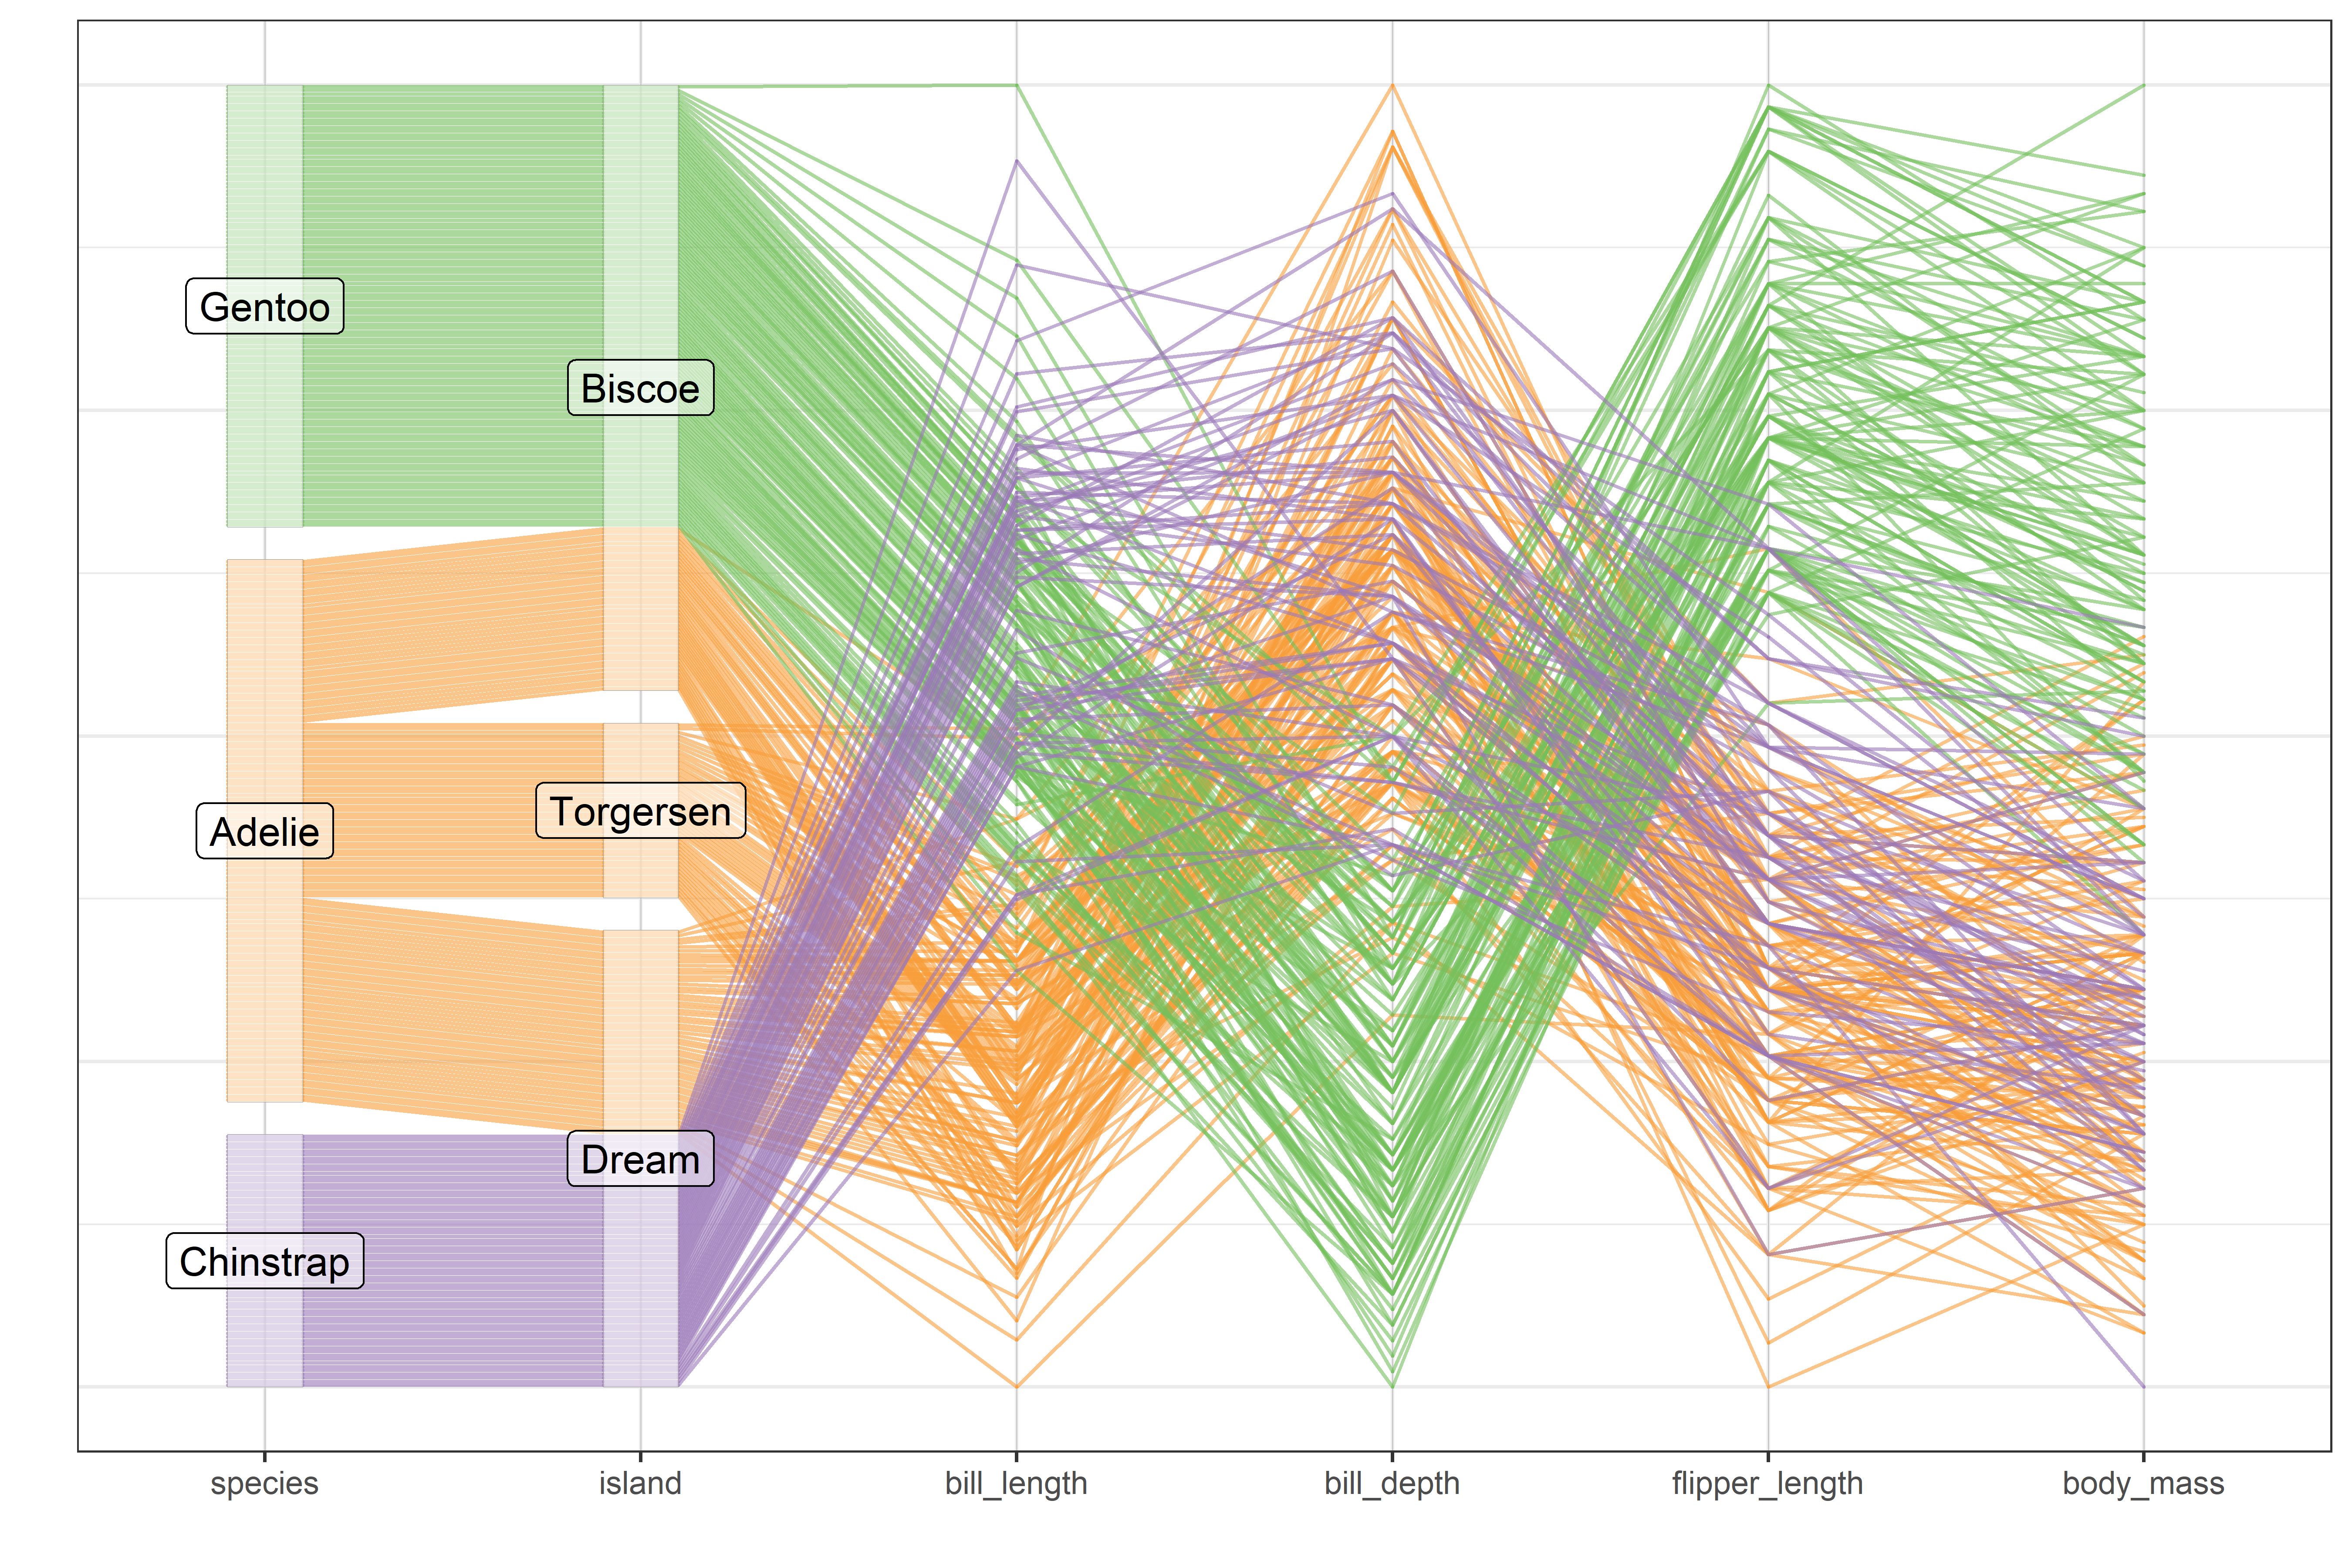
\includegraphics[width=18in,height=\textheight]{figs/fig-peng-ggpcp2-1.png}
\end{center}

This plot emphasizes the relation between penguin species and the island
where they were observed and then shows the values of the quantitative
body size measurements.

\section{Animated tours}\label{animated-tours}

In the mid 17\(^{th}\) to early 19\(^{th}\)-century the \textbf{Grand
Tour} became a coming-of-age custom for young Europeans (mainly British
nobility and landed gentry) of sufficient rank and means to undertake a
journey to the principal sites of Europe (Paris, Geneva, Rome, Athens,
\ldots) to complete their education by learning something of the
cultural legacies in history, art, and music from antiquity to the
Renaissance. Thereby, they could gain a wider appreciation of history
and be prepared to play a role in polite society or in their chosen
endeavors.

Travels in high-dimensional data space might be less thrilling than a
journey from London through Paris and Millan to Rome. Yet, in both cases
it is useful to think of the path taken, and what might be seen along
the way. But there are different kinds of tours. We might simply take a
meandering tour, exploring all the way, or want to plan a tour to see
the most interesting sites in travel or have a tour guided by an expert.
Similarly in data space, we might travel randomly to see what we can
find or be guided to find interesting features such as clusters,
outliers or non-linear relations in data.

Following the demonstration in PRIM-9 (\textbf{?@sec-discoveries}) of
exploring multidimensional data space by rotation Asimov
(\citeproc{ref-Asimov:85}{1985}) developed the idea of the \emph{grand
tour}, a computer method for viewing multivariate statistical data via
orthogonal projections onto an animated sequence of low-dimensional
subspaces, like a movie. In contrast to a scatterplot matrix which shows
a static view of a data cloud projected onto all pairwise variable axes,
a statistical tour is like the view of an eye moving smoothly in
high-dimensional space, capturing what it sees from a given location
onto the 2-d plane of the computer screen.

More generally, statistical tours are a type of dynamic projections onto
orthogonal axes (called a \emph{basis}) that embed data in a
\(p\)−dimensional space into a \(d\)−dimensional viewing subspace.
Typically, \(d=2\), and the result is displayed as scatterplots,
together with vectors representing the projections of the data variables
in this space. But the projected data can be rendered in 1-d as
densities or histograms, or in other number of dimensions as glyphs, or
even as parallel coordinate plots. The essential idea is that we can
define, and animate, a \emph{tour path} as a smooth sequence of such
projections over small changes to the projection basis, which gives the
orientation of the data in the viewing space.

\subsection{Projections}\label{projections}

The idea of a projection is fundamental to touring methods and other
visualizations of high-D data, so it is useful to understand what a
projection is. Quite simply, you can think of a projection as the shadow
of an object or cloud of points. This is nicely illustrated by the cover
image (Figure~\ref{fig-cover-GBE}) used for Douglas Hofstadter's
(\citeproc{ref-Hofstadter1979}{1979}) \emph{Gödel, Bach and Escher}
which shows 3D solid shapes illuminated by light sources so their
shadows form the letters G, B and E projected onto the planes formed by
pairs of the three coordinate axes. The set of three 2D views is
essentially the same that we see in a scatterplot matrix, where a 3D
dataset is portrayed by the set of shadows of the points on planes
formed by pairs of coordinate axes.

\begin{figure}

\centering{

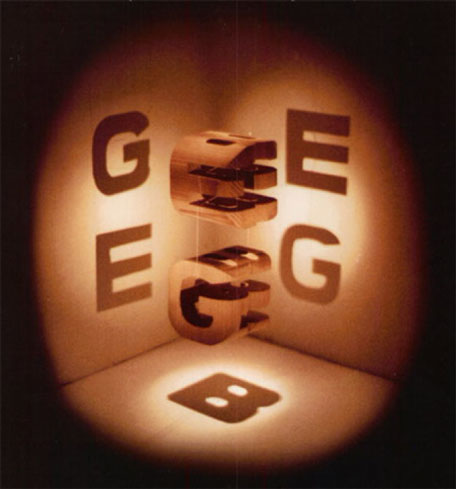
\includegraphics[width=0.4\textwidth,height=\textheight]{images/Cover-GBE.png}

}

\caption{\label{fig-cover-GBE}The cover image from Hofstadter
(\citeproc{ref-Hofstadter1979}{1979}) illustrates how projections are
shadows of an object cast by a light from a given direction.}

\end{figure}%

In the simplest case, a data point \(\mathbf{x} = (x_1, x_2)\) in two
dimensions can be represented geometrically as a vector from the origin
as shown in Figure~\ref{fig-projection}. This point can be projected on
any one-dimensional axis \(\mathbf{p}\) by dropping a line perpendicular
to \(\mathbf{p}\), which is the idea of a shadow. Mathematically, this
is calculated as the product
\(\mathbf{x}^\mathsf{T} \mathbf{p} = x_1 p_1 + x_2 p_2\) and suitably
normalized to give the correct length. \ldots{}

\begin{figure}

\centering{

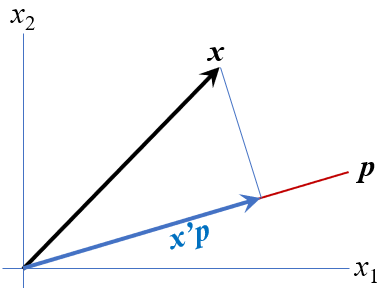
\includegraphics[width=0.4\textwidth,height=\textheight]{images/projection.png}

}

\caption{\label{fig-projection}Projection of a point \textbf{x} onto a
direction or axis \textbf{p}.}

\end{figure}%

More generally, a projection of an \((n \times p)\) data matrix
\(\mathbf{X}\) representing \(n\) observations in \(p\) dimensions onto
a \(d\)-dimensional viewing space \(\mathbf{Y}_{n \times d}\) is
represented by a \(p \times d\) projection matrix \(\mathbf{P}\) as
\(\mathbf{Y} = \mathbf{X} \mathbf{P}\), where the columns of
\(\mathbf{P}\) are orthogonal and of unit length,i.e.,
\(\mathbf{P}^\mathsf{T} \mathbf{P} = \mathbf{I}_{(d \times d)}\).

For example, to project a data matrix \(\mathbf{X}\) in three dimensions
onto a 2D plane, we would multiply it by a \((3 \times 2)\) orthonormal
matrix \(\mathbf{P}\). The matrix \(\mathbf{P}_1\) below simply selects
the first two columns of \(\mathbf{X}\).\footnote{This example was
  modified from one used by D. Cook et al.
  (\citeproc{ref-Cook-etal-2008}{2008}).}

\[
\mathbf{X} =
\begin{bmatrix} 
    0 & 0 & 0 \\ 
    0 & 0 & 10 \\ 
    0 & 10 & 0 \\ 
    0 & 10 & 10 \\ 
    10 & 0 & 0 \\ 
    10 & 0 & 10 \\ 
    10 & 10 & 0 \\ 
    10 & 10 & 10 \\ 
 \end{bmatrix}_{8 \times 3}
 ;\;
 \mathbf{P_1} =
 \begin{bmatrix} 
    1 & 0 \\ 
    0 & 1 \\ 
    0 & 0 \\ 
 \end{bmatrix}_{3 \times 2} 
 \;\Rightarrow\quad
 \mathbf{Y} = \mathbf{X} \; \mathbf{P_1} =
 \begin{bmatrix} 
    0 & 0 \\ 
    0 & 0 \\ 
    0 & 10 \\ 
    0 & 10 \\ 
    10 & 0 \\ 
    10 & 0 \\ 
    10 & 10 \\ 
    10 & 10 \\ 
 \end{bmatrix}_{8 \times 2} 
\] An oblique projection using all three dimensions is given by
\(\mathbf{P_2}\) below. This produces a new 2D view in \(\mathbf{Y}\):
\[
 \mathbf{P_2} =
\begin{bmatrix} 
    0.71 & -0.42 \\ 
    0.71 & 0.42 \\ 
    0 & 0.84 \\ 
 \end{bmatrix}_{3 \times 2}
 \quad\Rightarrow\quad
 \mathbf{Y} = \mathbf{X} \; \mathbf{P_2} =
\begin{bmatrix} 
    0 & 0 \\ 
    0 & 8.4 \\ 
    7.1 & 4.2 \\ 
    7.1 & 12.6 \\ 
    7.1 & -4.2 \\ 
    7.1 & 4.2 \\ 
    14.2 & 0 \\ 
    14.2 & 8.4 \\ 
 \end{bmatrix} 
\]

The columns in \(\mathbf{Y}\) are simply the linear combinations of
those of \(\mathbf{X}\) using the weights in each column of
\(\mathbf{P_2}\)

\begin{eqnarray*}
\mathbf{y}_1 & = & 0.71 \mathbf{x}_1 + 0.71 \mathbf{x}_2 + 0 \mathbf{x}_3\\
\mathbf{y}_2 & = & -0.42 \mathbf{x}_1 + 0.42 \mathbf{x}_2 + 0.84 \mathbf{x}_3 \\
\end{eqnarray*}

\begin{Shaded}
\begin{Highlighting}[]
\NormalTok{vals }\OtherTok{\textless{}{-}} \FunctionTok{c}\NormalTok{(}\DecValTok{0}\NormalTok{, }\DecValTok{10}\NormalTok{)}
\NormalTok{X }\OtherTok{\textless{}{-}} \FunctionTok{expand.grid}\NormalTok{(}\AttributeTok{x1 =}\NormalTok{ vals, }\AttributeTok{x2=}\NormalTok{vals, }\AttributeTok{x3=}\NormalTok{vals) }\SpecialCharTok{|\textgreater{}} \FunctionTok{as.matrix}\NormalTok{()}

\CommentTok{\# project on just x1, x2 plane}
\NormalTok{P1 }\OtherTok{\textless{}{-}} \FunctionTok{rbind}\NormalTok{(}\FunctionTok{diag}\NormalTok{(}\DecValTok{2}\NormalTok{), }\FunctionTok{c}\NormalTok{(}\DecValTok{0}\NormalTok{,}\DecValTok{0}\NormalTok{))}
\NormalTok{Y1 }\OtherTok{\textless{}{-}}\NormalTok{ X }\SpecialCharTok{\%*\%}\NormalTok{ P1}

\CommentTok{\# oblique projection}
\NormalTok{P2 }\OtherTok{\textless{}{-}} \FunctionTok{matrix}\NormalTok{(}\FunctionTok{c}\NormalTok{(}\FloatTok{0.71}\NormalTok{, }\FloatTok{0.71}\NormalTok{, }\DecValTok{0}\NormalTok{, }\SpecialCharTok{{-}}\FloatTok{0.42}\NormalTok{, .}\DecValTok{42}\NormalTok{, }\FloatTok{0.84}\NormalTok{), }\AttributeTok{ncol=}\DecValTok{2}\NormalTok{)}
\NormalTok{Y2 }\OtherTok{\textless{}{-}}\NormalTok{ X }\SpecialCharTok{\%*\%}\NormalTok{ P2}
\end{Highlighting}
\end{Shaded}

In this example, the matrix \(\mathbf{X}\) consists of 8 points at the
vertices of a cube of size 10, as shown in
Figure~\ref{fig-proj-combined} (a). The projections
\(\mathbf{Y}_1 = \mathbf{P}_1 \mathbf{X}\) and
\(\mathbf{Y}_2 = \mathbf{P}_2 \mathbf{X}\) are shown in panels (b) and
(c). To make it easier to relate the points in different views, shapes
and colors are assigned so that each point has a unique combination of
these attributes.\footnote{Plot shapes given by \texttt{pch\ =\ 15:18}
  correspond to: filled square (15), filled circle (16), filled triangle
  point-up (17), filled diamond (18).}

\begin{Shaded}
\begin{Highlighting}[]
\NormalTok{pch }\OtherTok{\textless{}{-}} \FunctionTok{rep}\NormalTok{(}\DecValTok{15}\SpecialCharTok{:}\DecValTok{18}\NormalTok{, }\AttributeTok{times =} \DecValTok{2}\NormalTok{)}
\NormalTok{colors }\OtherTok{\textless{}{-}} \FunctionTok{c}\NormalTok{(}\StringTok{"red"}\NormalTok{, }\StringTok{"blue"}\NormalTok{, }\StringTok{"darkgreen"}\NormalTok{, }\StringTok{"brown"}\NormalTok{)}
\NormalTok{col }\OtherTok{\textless{}{-}} \FunctionTok{rep}\NormalTok{(colors, }\AttributeTok{each =} \DecValTok{2}\NormalTok{)}
\FunctionTok{data.frame}\NormalTok{(X, pch, col)}
\CommentTok{\#\textgreater{}   x1 x2 x3 pch       col}
\CommentTok{\#\textgreater{} 1  0  0  0  15       red}
\CommentTok{\#\textgreater{} 2 10  0  0  16       red}
\CommentTok{\#\textgreater{} 3  0 10  0  17      blue}
\CommentTok{\#\textgreater{} 4 10 10  0  18      blue}
\CommentTok{\#\textgreater{} 5  0  0 10  15 darkgreen}
\CommentTok{\#\textgreater{} 6 10  0 10  16 darkgreen}
\CommentTok{\#\textgreater{} 7  0 10 10  17     brown}
\CommentTok{\#\textgreater{} 8 10 10 10  18     brown}
\end{Highlighting}
\end{Shaded}

\begin{figure}

\centering{

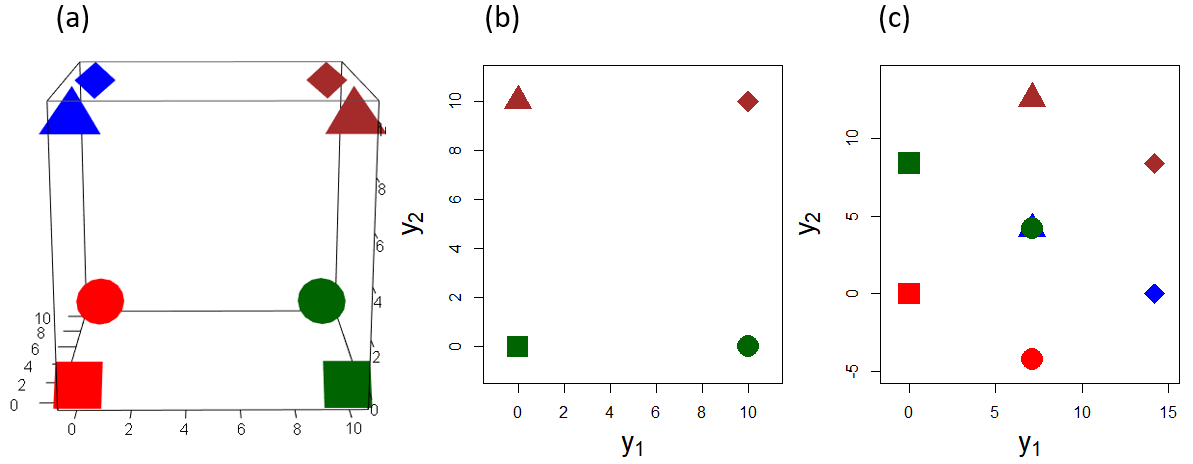
\includegraphics[width=1\textwidth,height=\textheight]{images/proj-combined.png}

}

\caption{\label{fig-proj-combined}\textbf{Projection example}: (a) The 8
points in \textbf{X} form a cube of size 10; (b) the projection by
\textbf{P1} is the view ignoring \textbf{x3} (two points coincide at
each vertex); (c) the projection by \textbf{P2} is an oblique view.}

\end{figure}%

But, if we are traveling in the projection space of \(\mathbf{Y}\), we
need some signposts to tell us how the new dimensions relate to those of
\(\mathbf{X}\). The answer is provided simply by plotting the rows of
\(\mathbf{P}\) as vectors, as shown in Figure~\ref{fig-proj-vectors}. In
these plots, each row of \(\mathbf{P}_1\) and \(\mathbf{P}_2\) appears
as a vector from the origin. It's direction shows the contribution each
of \(\mathbf{x}_1, \mathbf{x}_2, \mathbf{x}_3\) make to the new
coordinates \(\mathbf{y}_1\) and \(\mathbf{y}_2\).

In \(\mathbf{P}_1\), the projected variable \(\mathbf{y}_1\) is related
only to \(\mathbf{x}_1\), while \(\mathbf{y}_2\) is related only to
\(\mathbf{x}_2\) \(\mathbf{x}_3\) makes no contribution, and appears at
the origin. However in the projection given by \(\mathbf{P}_2\),
\(\mathbf{x}_1\) and \(\mathbf{x}_2\) make the same contribution to
\(\mathbf{y}_1\), while \(\mathbf{x}_3\) has no contribution to that
horizontal axis. The vertical axis, \(\mathbf{y}_2\) here is completely
aligned with \(\mathbf{x}_3\); \(\mathbf{x}_1\) and \(\mathbf{x}_2\)
have vertical components that are half of that for \(\mathbf{x}_3\) in
absolute value.

\begin{Shaded}
\begin{Highlighting}[]
\FunctionTok{library}\NormalTok{(matlib)}
\NormalTok{op }\OtherTok{\textless{}{-}} \FunctionTok{par}\NormalTok{(}\AttributeTok{mar=}\FunctionTok{c}\NormalTok{(}\DecValTok{4}\NormalTok{, }\DecValTok{5}\NormalTok{, }\DecValTok{1}\NormalTok{, }\DecValTok{1}\NormalTok{)}\SpecialCharTok{+}\NormalTok{.}\DecValTok{1}\NormalTok{)}
\NormalTok{xlim }\OtherTok{\textless{}{-}}\NormalTok{ ylim }\OtherTok{\textless{}{-}} \FunctionTok{c}\NormalTok{(}\SpecialCharTok{{-}}\FloatTok{1.1}\NormalTok{, }\FloatTok{1.1}\NormalTok{)}
\NormalTok{axes.x }\OtherTok{\textless{}{-}} \FunctionTok{c}\NormalTok{(}\SpecialCharTok{{-}}\DecValTok{1}\NormalTok{, }\DecValTok{1}\NormalTok{, }\ConstantTok{NA}\NormalTok{, }\DecValTok{0}\NormalTok{, }\DecValTok{0}\NormalTok{)}
\NormalTok{axes.y }\OtherTok{\textless{}{-}} \FunctionTok{c}\NormalTok{(}\DecValTok{0}\NormalTok{, }\DecValTok{0}\NormalTok{, }\ConstantTok{NA}\NormalTok{, }\SpecialCharTok{{-}}\DecValTok{1}\NormalTok{, }\DecValTok{1}\NormalTok{)}
\NormalTok{labs }\OtherTok{\textless{}{-}} \FunctionTok{c}\NormalTok{(}\FunctionTok{expression}\NormalTok{(x[}\DecValTok{1}\NormalTok{]), }\FunctionTok{expression}\NormalTok{(x[}\DecValTok{2}\NormalTok{]), }\FunctionTok{expression}\NormalTok{(x[}\DecValTok{3}\NormalTok{]))}
\FunctionTok{plot}\NormalTok{(xlim, ylim, }\AttributeTok{type =} \StringTok{"n"}\NormalTok{, }\AttributeTok{asp=}\DecValTok{1}\NormalTok{,}
     \AttributeTok{xlab =} \FunctionTok{expression}\NormalTok{(y[}\DecValTok{1}\NormalTok{]), }\AttributeTok{ylab =} \FunctionTok{expression}\NormalTok{(y[}\DecValTok{2}\NormalTok{]),}
     \AttributeTok{cex.lab =} \FloatTok{1.8}\NormalTok{)}
\FunctionTok{circle}\NormalTok{(}\DecValTok{0}\NormalTok{, }\DecValTok{0}\NormalTok{, }\DecValTok{1}\NormalTok{, }\AttributeTok{col =} \FunctionTok{adjustcolor}\NormalTok{(}\StringTok{"skyblue"}\NormalTok{, }\AttributeTok{alpha =} \FloatTok{0.2}\NormalTok{))}
\FunctionTok{lines}\NormalTok{(axes.x, axes.y, }\AttributeTok{col =} \StringTok{"grey"}\NormalTok{)}
\FunctionTok{vectors}\NormalTok{(P1, }\AttributeTok{labels =}\NormalTok{ labs, }\AttributeTok{cex.lab =} \FloatTok{1.8}\NormalTok{, }\AttributeTok{lwd =} \DecValTok{3}\NormalTok{, }\AttributeTok{pos.lab =} \FunctionTok{c}\NormalTok{(}\DecValTok{4}\NormalTok{, }\DecValTok{2}\NormalTok{, }\DecValTok{1}\NormalTok{))}

\FunctionTok{plot}\NormalTok{(xlim, ylim, }\AttributeTok{type =} \StringTok{"n"}\NormalTok{, }\AttributeTok{asp=}\DecValTok{1}\NormalTok{,}
     \AttributeTok{xlab =} \FunctionTok{expression}\NormalTok{(y[}\DecValTok{1}\NormalTok{]), }\AttributeTok{ylab =} \FunctionTok{expression}\NormalTok{(y[}\DecValTok{2}\NormalTok{]),}
     \AttributeTok{cex.lab =} \FloatTok{1.8}\NormalTok{)}
\FunctionTok{circle}\NormalTok{(}\DecValTok{0}\NormalTok{, }\DecValTok{0}\NormalTok{, }\DecValTok{1}\NormalTok{, }\AttributeTok{col =} \FunctionTok{adjustcolor}\NormalTok{(}\StringTok{"skyblue"}\NormalTok{, }\AttributeTok{alpha =} \FloatTok{0.2}\NormalTok{))}
\FunctionTok{lines}\NormalTok{(axes.x, axes.y, }\AttributeTok{col =} \StringTok{"grey"}\NormalTok{)}
\FunctionTok{vectors}\NormalTok{(P2, }\AttributeTok{labels =}\NormalTok{ labs, }\AttributeTok{cex.lab =} \FloatTok{1.8}\NormalTok{, }\AttributeTok{lwd =} \DecValTok{3}\NormalTok{)}
\FunctionTok{par}\NormalTok{(op)}
\end{Highlighting}
\end{Shaded}

\begin{figure}%
\end{figure}%

\begin{figure}

\centering{

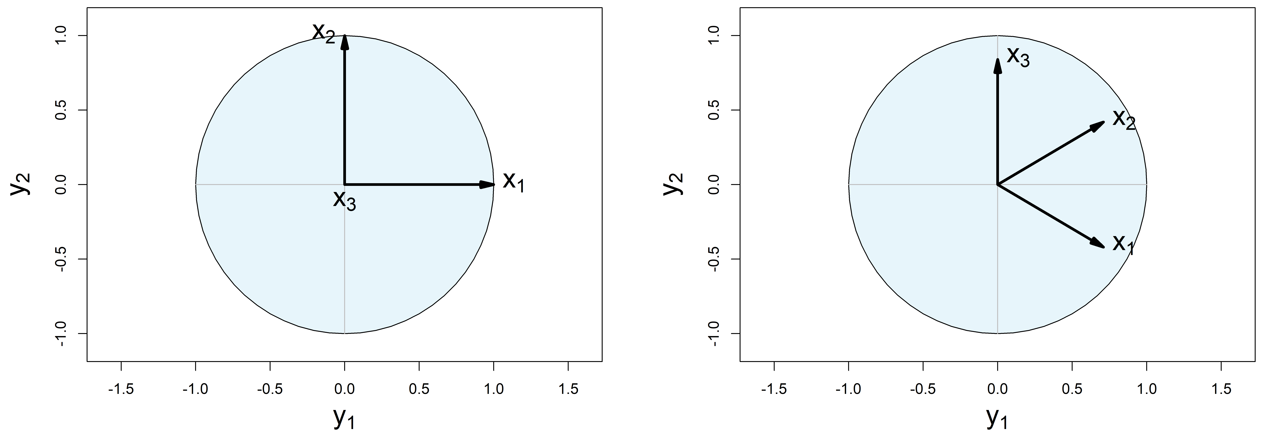
\includegraphics[width=1\textwidth,height=\textheight]{images/proj-vectors.png}

}

\caption{\label{fig-proj-vectors}\textbf{Variable vectors}: Data
variables viewed as vectors in the space of their projections. The
angles of the \textbf{x} vectors with respect to the \textbf{y}
coordinate axes show their relative contributions to each. The lengths
of the \textbf{x} vectors show the relative degree to which they are
represented in the space of \textbf{y}s. Left: the \textbf{P1}
projection; right: the \textbf{P2} projection.}

\end{figure}%

\subsubsection{Vector lengths}\label{vector-lengths}

In Figure~\ref{fig-proj-vectors}, the \textbf{lengths} of the
\(\mathbf{x}\) vectors reflect the relative degree to which each
variable is represented in the space of the projection, and this is
important for interpretation. For the \(\mathbf{P}_1\) projection,
\(\mathbf{x}_3\) is of length 0, while \(\mathbf{x}_1\) and
\(\mathbf{x}_2\) fill the unit circle. In the projection given by
\(\mathbf{P}_2\), all three \(\mathbf{x}\) are approximately the same
length.

In algebra, the length of a vector \(\mathbf{x}\) is
\(||\mathbf{x}|| = (\mathbf{x}^\mathsf{T} \mathbf{x})^{1/2} = \sqrt{\Sigma x_i^2}\),
the Euclidean distance of the tip of the vector from the origin. In R,
we calculate the lengths of row vectors in a projection matrix by
transposing and using \texttt{matlib::len()}.

\begin{Shaded}
\begin{Highlighting}[]
\NormalTok{P1 }\SpecialCharTok{|\textgreater{}} \FunctionTok{t}\NormalTok{() }\SpecialCharTok{|\textgreater{}}\NormalTok{ matlib}\SpecialCharTok{::}\FunctionTok{len}\NormalTok{()}
\CommentTok{\#\textgreater{} [1] 1 1 0}
\NormalTok{P2 }\SpecialCharTok{|\textgreater{}} \FunctionTok{t}\NormalTok{() }\SpecialCharTok{|\textgreater{}}\NormalTok{ matlib}\SpecialCharTok{::}\FunctionTok{len}\NormalTok{()}
\CommentTok{\#\textgreater{} [1] 0.825 0.825 0.840}
\end{Highlighting}
\end{Shaded}

\subsubsection{Joint-views}\label{joint-views}

To interpret such projections, we want to see \textbf{both} the
projected data and the signposts that tell us where we are in relation
to the original variables. To do this, we can overlay the variable
vectors represented by the rows of the projection matrix \(\mathbf{P}\)
onto plots like Figure~\ref{fig-proj-combined} (b) and
Figure~\ref{fig-proj-combined} (c) to see how the axes in a projection
relate to those in the data. To place these together on the same plot,
we can either center the columns of \(\mathbf{Y}\) at their means or
shift the the columns of \(\mathbf{P}\) to \texttt{colMeans(Y)}. It is
only the directions of the vectors that matters, so we are free to scale
their lengths by any convenient factor.

\begin{Shaded}
\begin{Highlighting}[]
\NormalTok{Y2s }\OtherTok{\textless{}{-}} \FunctionTok{scale}\NormalTok{(Y2, }\AttributeTok{scale=}\ConstantTok{FALSE}\NormalTok{)       }\CommentTok{\# center Y2}
\FunctionTok{plot}\NormalTok{(Y2s, }\AttributeTok{cex =} \DecValTok{3}\NormalTok{, }
     \AttributeTok{asp =} \DecValTok{1}\NormalTok{,}
     \AttributeTok{pch =}\NormalTok{ pch, }\AttributeTok{col =}\NormalTok{ col,}
     \AttributeTok{xlab =} \FunctionTok{expression}\NormalTok{(y[}\DecValTok{1}\NormalTok{]), }\AttributeTok{ylab =} \FunctionTok{expression}\NormalTok{(y[}\DecValTok{2}\NormalTok{]),}
     \AttributeTok{xlim =} \FunctionTok{c}\NormalTok{(}\SpecialCharTok{{-}}\DecValTok{10}\NormalTok{, }\DecValTok{10}\NormalTok{), }\AttributeTok{ylim =} \FunctionTok{c}\NormalTok{(}\SpecialCharTok{{-}}\DecValTok{10}\NormalTok{, }\DecValTok{10}\NormalTok{), }\AttributeTok{cex.lab =} \FloatTok{1.8}\NormalTok{)}
\NormalTok{r }\OtherTok{\textless{}{-}} \DecValTok{7}
\NormalTok{vecs }\OtherTok{\textless{}{-}}\NormalTok{ (r}\SpecialCharTok{*}\FunctionTok{diag}\NormalTok{(}\DecValTok{3}\NormalTok{) }\SpecialCharTok{\%*\%}\NormalTok{ P2)}
\FunctionTok{vectors}\NormalTok{(vecs, }\AttributeTok{labels =}\NormalTok{ labs, }\AttributeTok{cex.lab =} \FloatTok{1.8}\NormalTok{, }\AttributeTok{lwd =} \DecValTok{2}\NormalTok{)}
\FunctionTok{vectors}\NormalTok{(}\SpecialCharTok{{-}}\NormalTok{vecs, }\AttributeTok{labels =} \ConstantTok{NULL}\NormalTok{, }\AttributeTok{lty =} \DecValTok{1}\NormalTok{, }\AttributeTok{angle =} \DecValTok{1}\NormalTok{, }\AttributeTok{col =} \StringTok{"gray"}\NormalTok{)}
\end{Highlighting}
\end{Shaded}

The plot in Figure~\ref{fig-proj-P2-vec} illustrates this, centering
\(\mathbf{Y}\), and multiplying the vectors in \(\mathbf{P}\) by 7. To
check your understanding, try to see if you can relate what is shown in
this plot to the 3D plot in Figure~\ref{fig-proj-combined} (a).

\begin{figure}

\centering{

\includegraphics[width=0.5\textwidth,height=\textheight]{images/proj-P2-vec.png}

}

\caption{\label{fig-proj-P2-vec}The \textbf{P2} projection of the data
showing vectors for the original variables in the space of \textbf{Y}.}

\end{figure}%

The idea of viewing low-dimensional projections of data together with
vectors representing the contributions of the original variables to the
dimensions shown in a display is also the basis of \textbf{biplot}
techniques (Section~\ref{sec-biplot}) we will use in relation to
principal components analysis.

\subsection{Touring methods}\label{touring-methods}

The trick of statistical touring methods is to generate a smooth
sequence of interpolated projections \(\mathbf{P}_{(t)}\) indexed by
time \(t\),
\(\mathbf{P}_{(1)}, \mathbf{P}_{(2)}, \mathbf{P}_{(3)}, \dots, \mathbf{P}_{(T)}\).
This gives a path of views
\(\mathbf{Y}_{(t)} = \mathbf{X} \mathbf{P}_{(t)}\), that can be animated
in successive frames, as shown schematically in
Figure~\ref{fig-peng-tourr-diagram}.

\begin{figure}

\centering{

\includegraphics[width=0.9\textwidth,height=\textheight]{images/peng-tourr-diagram.png}

}

\caption{\label{fig-peng-tourr-diagram}\textbf{Interpolations}:
Illustration of a grand tour of interpolations of projection planes
showing 2D scatterplots of the Penguin dataset. The seqeunce of views
moves smoothly from an initial frame \textbf{P(1)} to a final frame
\textbf{P(T)} where the penguin species are widely separated.}

\end{figure}%

Asimov's (\citeproc{ref-Asimov:85}{1985}) original idea of the grand
tour was that of a random path, picking orthogonal projections
\(\mathbf{P}_{(i)}\) at random. Given enough time, the grand tour gives
a space-filling path and would eventually show every possible projection
of the data. But it does so smoothly, by interpolating from one
projection to the next. In the travel analogy, the path by road from
London to Paris might go smoothly through Kent to Dover, thence via
Amiens and Beauvais before reaching Paris. By air, the tour would follow
a smoother \emph{geodesic} path, and this is what the grand tour does.
The sense in watching an animation of a statistical grand tour is that
of continuous motion. The grand tour algorithm is described in detail by
Buja et al. (\citeproc{ref-Buja-etal-2005}{2005}) and D. Cook et al.
(\citeproc{ref-Cook-etal-2008}{2008}).

\subsubsection{Guided tours}\label{guided-tours}

The next big idea was that rather than traveling randomly in projection
space one could take a \emph{guided tour}, following a path that leads
to ``interesting projections'', such as those that reveal clusters, gaps
in data space or outliers. This idea, called \emph{projection pursuit}
(\citeproc{ref-Cook-etal-1995}{D. Cook et al., 1995}), works by defining
a measure of interestingness of a data projection. In a guided tour, the
next projection is chosen to increase that index, so over time the
projection moves toward one that is maximizes that index.

In the time since Asimov (\citeproc{ref-Asimov:85}{1985}), there have
been many implementations of touring visualization methods. XGobi
(\citeproc{ref-Swayne-etal-1998}{Swayne et al., 1998}) for X-Windows
displays on Linux systems provided a test-bed for dynamic, interactive
graphic methods; it's successor, GGobi
(\citeproc{ref-CookSwayne:2007}{D. Cook \& Swayne, 2007};
\citeproc{ref-Swayne-etal-2003}{Swayne et al., 2003}) extended the range
of touring methods to include a wider variety of projection pursuit
indices.

\subsubsection{\texorpdfstring{\texttt{tourr}
package}{tourr package}}\label{tourr-package}

The current state of art is best captured in the \textbf{tourr} package
for R (\citeproc{ref-Wickham-etal-2011}{Wickham et al., 2011};
\citeproc{ref-R-tourr}{Wickham \& Cook, 2024}). It defines a tour to
consist of three components:

\begin{itemize}
\tightlist
\item
  \textbf{data}: An \((n \times p)\) numerical data matrix to be viewed.
\item
  \textbf{path}: A tour path function that produces a smoothed sequence
  of projection matrices \(\mathbf{P}_{(p \times d)}\) in \(d\).
  dimensions, for example \texttt{grand\_tour(d\ =\ 2)} or
  \texttt{guided\_tour(index\ =\ holes)}.
\item
  \textbf{display}: A function that renders the projected data, for
  example \texttt{display\_xy()} for a scatterplot,
  \texttt{display\_depth()} for a 3D plot with simulated depth, or
  \texttt{display\_pcp()} for a parallel coordinates plots
\end{itemize}

This very nicely separates the aspects of a tour, and allows one to
think of and define new tour path methods and display methods. The
package defines two general tour functions: \texttt{animate()} produces
a real-time animation on a display device and \texttt{render()} saves
image frames to disk, such as a \texttt{.gif} file.

\begin{Shaded}
\begin{Highlighting}[]
\FunctionTok{animate}\NormalTok{(data, tour\_path, display\_method)}
\FunctionTok{render}\NormalTok{(data, tour\_path, display\_method)}
\end{Highlighting}
\end{Shaded}

The \textbf{tourr} package provides a wide range of tour path methods
and display methods:

\begin{Shaded}
\begin{Highlighting}[]
\CommentTok{\# tour path methods}
\FunctionTok{grep}\NormalTok{(}\StringTok{"\_tour$"}\NormalTok{, }\FunctionTok{lsf.str}\NormalTok{(}\StringTok{"package:tourr"}\NormalTok{), }\AttributeTok{value =} \ConstantTok{TRUE}\NormalTok{)}
\CommentTok{\#\textgreater{}  [1] "dependence\_tour"     "frozen\_guided\_tour" }
\CommentTok{\#\textgreater{}  [3] "frozen\_tour"         "grand\_tour"         }
\CommentTok{\#\textgreater{}  [5] "guided\_anomaly\_tour" "guided\_section\_tour"}
\CommentTok{\#\textgreater{}  [7] "guided\_tour"         "little\_tour"        }
\CommentTok{\#\textgreater{}  [9] "local\_tour"          "new\_tour"           }
\CommentTok{\#\textgreater{} [11] "planned\_tour"        "planned2\_tour"      }
\CommentTok{\#\textgreater{} [13] "radial\_tour"}

\CommentTok{\# display methods}
\FunctionTok{grep}\NormalTok{(}\StringTok{"display\_"}\NormalTok{, }\FunctionTok{lsf.str}\NormalTok{(}\StringTok{"package:tourr"}\NormalTok{), }\AttributeTok{value =} \ConstantTok{TRUE}\NormalTok{)}
\CommentTok{\#\textgreater{}  [1] "display\_andrews"   "display\_density2d" "display\_depth"    }
\CommentTok{\#\textgreater{}  [4] "display\_dist"      "display\_faces"     "display\_groupxy"  }
\CommentTok{\#\textgreater{}  [7] "display\_idx"       "display\_image"     "display\_pca"      }
\CommentTok{\#\textgreater{} [10] "display\_pcp"       "display\_sage"      "display\_scatmat"  }
\CommentTok{\#\textgreater{} [13] "display\_slice"     "display\_stars"     "display\_stereo"   }
\CommentTok{\#\textgreater{} [16] "display\_trails"    "display\_xy"}
\end{Highlighting}
\end{Shaded}

Tour path methods take a variety of optional arguments to specify the
detailed behavior of the method. For example, most allow you to specify
the number of dimension (\texttt{d\ =}) of the projections. The
\texttt{guided\_tour()} is of particular interest here.

\begin{Shaded}
\begin{Highlighting}[]
\FunctionTok{args}\NormalTok{(guided\_tour)}
\CommentTok{\#\textgreater{} function (index\_f, d = 2, alpha = 0.5, cooling = 0.99, max.tries = 25, }
\CommentTok{\#\textgreater{}     max.i = Inf, search\_f = search\_geodesic, n\_sample = 100, }
\CommentTok{\#\textgreater{}     ...) }
\CommentTok{\#\textgreater{} NULL}
\end{Highlighting}
\end{Shaded}

In this, \texttt{index\_f} specifies a function that the method tries to
optimize on its path and package defines four indices:

\begin{itemize}
\tightlist
\item
  Holes (\texttt{holes()}): This is sensitive to projections with
  separated clusters of points, with few points near the origin
\item
  Central mass (\texttt{cmass()}): Sensitive to projections with lots of
  points in the center, but perhaps with some outliers
\item
  Linear discriminant analysis (\texttt{lda\_pp()}): For data with a
  grouping factor, optimizes a measure of separation of the group means
  as in MANOVA or linear discriminant analysis.
\item
  PDA analysis (\texttt{pda\_pp()}): A penalized version of
  \texttt{lda\_pp()} for cases of large \(p\) relative to sample size
  \(n\) (\citeproc{ref-LeeCook-2009}{E.-K. Lee \& Cook, 2009}).
\end{itemize}

In addition, there is now a \texttt{guided\_anomaly\_tour()} that looks
for the best projection of observations that are outside the data
ellipsoid, finding a view showing observations with large Mahalanobis
distances from the centroid.

\subsubsection{Penguin tours}\label{penguin-tours}

Penguins are a traveling species. They make yearly travels inland to
breeding sites in early spring, repeating the patterns of their
ancestors. Near the beginning of summer, adult penguins and their chicks
return to the sea and spend the rest of the summer feeding there
(\citeproc{ref-Black-etal-2018}{Black et al., 2018}). If they were also
data scientists, they might wonder about the relations among among their
cousins of different species and take a tour of their
measurements\ldots{}

For example, using the Penguins dataset, the following calls produce
grand tours in 2, 3, and 4 dimensions. The 2D tour is displayed as a
scatterplot, the 3D tour using simulated depth as shown by variation in
point size and transparency, and the 4D tour is shown using a parallel
coordinate plot.

\begin{Shaded}
\begin{Highlighting}[]
\FunctionTok{data}\NormalTok{(peng, }\AttributeTok{package =} \StringTok{"heplots"}\NormalTok{)}
\NormalTok{peng\_scaled }\OtherTok{\textless{}{-}} \FunctionTok{scale}\NormalTok{(peng[,}\DecValTok{3}\SpecialCharTok{:}\DecValTok{6}\NormalTok{])}
\FunctionTok{colnames}\NormalTok{(peng\_scaled) }\OtherTok{\textless{}{-}} \FunctionTok{c}\NormalTok{(}\StringTok{"BL"}\NormalTok{, }\StringTok{"BD"}\NormalTok{, }\StringTok{"FL"}\NormalTok{, }\StringTok{"BM"}\NormalTok{)}

\FunctionTok{animate}\NormalTok{(peng\_scaled, }\FunctionTok{grand\_tour}\NormalTok{(}\AttributeTok{d =} \DecValTok{2}\NormalTok{), }\FunctionTok{display\_xy}\NormalTok{())}
\FunctionTok{animate}\NormalTok{(peng\_scaled, }\FunctionTok{grand\_tour}\NormalTok{(}\AttributeTok{d =} \DecValTok{3}\NormalTok{), }\FunctionTok{display\_depth}\NormalTok{())}
\FunctionTok{animate}\NormalTok{(peng\_scaled, }\FunctionTok{grand\_tour}\NormalTok{(}\AttributeTok{d =} \DecValTok{4}\NormalTok{), }\FunctionTok{display\_pcp}\NormalTok{())}
\end{Highlighting}
\end{Shaded}

\begin{figure}

\begin{minipage}{0.33\linewidth}

\centering{

\includegraphics[width=0.33\textwidth,height=\textheight]{images/tours/peng-tour-demo1.png}

}

\subcaption{\label{fig-peng-tour-demo-1}2D, scatterplot}

\end{minipage}%
%
\begin{minipage}{0.33\linewidth}

\centering{

\includegraphics[width=0.33\textwidth,height=\textheight]{images/tours/peng-tour-demo2.png}

}

\subcaption{\label{fig-peng-tour-demo-2}3D, simulated depth}

\end{minipage}%
%
\begin{minipage}{0.33\linewidth}

\centering{

\includegraphics[width=0.33\textwidth,height=\textheight]{images/tours/peng-tour-demo3.png}

}

\subcaption{\label{fig-peng-tour-demo-3}4D, parallel coordinates plot}

\end{minipage}%

\caption{\label{fig-peng-tour-demo}Grand tours of the penguin dataset in
2, 3, and 4 dimensions using different \texttt{display\_*()} methods.}

\end{figure}%

To illustrate, I'll start with a grand tour designed to explore this 4D
space of penguins. I'll abbreviate the variables to two characters,
``BL'' = \texttt{bill\_length}, ``BD'' = \texttt{bill\_depth}, ``FL'' =
\texttt{flipper\_length}, and ``BM'' = \texttt{body\_mass} and identify
the penguin species using point shape (\texttt{pch}) and color
(\texttt{col}).

As you watch this pay attention to the separation of the species and any
other interesting features. What do you see?

\begin{Shaded}
\begin{Highlighting}[]
\FunctionTok{data}\NormalTok{(peng, }\AttributeTok{package =} \StringTok{"heplots"}\NormalTok{)}
\NormalTok{peng\_scaled }\OtherTok{\textless{}{-}} \FunctionTok{scale}\NormalTok{(peng[,}\DecValTok{3}\SpecialCharTok{:}\DecValTok{6}\NormalTok{])}
\FunctionTok{colnames}\NormalTok{(peng\_scaled) }\OtherTok{\textless{}{-}} \FunctionTok{c}\NormalTok{(}\StringTok{"BL"}\NormalTok{, }\StringTok{"BD"}\NormalTok{, }\StringTok{"FL"}\NormalTok{, }\StringTok{"BM"}\NormalTok{)}

\NormalTok{pch }\OtherTok{\textless{}{-}} \FunctionTok{c}\NormalTok{(}\DecValTok{15}\NormalTok{, }\DecValTok{16}\NormalTok{, }\DecValTok{17}\NormalTok{)[peng}\SpecialCharTok{$}\NormalTok{species] }
\NormalTok{cex }\OtherTok{=} \FloatTok{1.2}

\FunctionTok{set.seed}\NormalTok{(}\DecValTok{1234}\NormalTok{)}
\FunctionTok{animate}\NormalTok{(peng\_scaled,}
        \AttributeTok{tour\_path =} \FunctionTok{grand\_tour}\NormalTok{(}\AttributeTok{d=}\DecValTok{2}\NormalTok{),}
        \FunctionTok{display\_xy}\NormalTok{(}\AttributeTok{col =}\NormalTok{ peng}\SpecialCharTok{$}\NormalTok{species,}
                   \AttributeTok{palette =} \FunctionTok{peng.colors}\NormalTok{(}\StringTok{"dark"}\NormalTok{),}
                   \AttributeTok{pch =}\NormalTok{ pch, }\AttributeTok{cex =}\NormalTok{ cex,}
                   \AttributeTok{axis.col =} \StringTok{"black"}\NormalTok{, }
                   \AttributeTok{axis.text.col =} \StringTok{"black"}\NormalTok{, }
                   \AttributeTok{axis.lwd =} \FloatTok{1.5}\NormalTok{))}
\end{Highlighting}
\end{Shaded}

Figure~\ref{fig-peng-tour-grand-frames} shows three frames from this
movie. The first (a) is the initial frame that shows the projection in
the plane of bill depth and bill length. The variable vectors indicate
that bill length differentiates Adelie penguins from the others. In
frame (b), the three species are widely separated, with bill depth
distinguishing Gentoo from the others. In frame (c) the three species
are largely mixed, but two points stand out as outliers, with
exceptionally long bills compared to the rest.

\begin{figure}

\begin{minipage}{0.33\linewidth}

\centering{

\includegraphics[width=1\textwidth,height=\textheight]{images/tours/peng-grand-tour1.png}

}

\subcaption{\label{fig-peng-tour-grand-frames-1}Initial frame}

\end{minipage}%
%
\begin{minipage}{0.33\linewidth}

\centering{

\includegraphics[width=1\textwidth,height=\textheight]{images/tours/peng-grand-tour2.png}

}

\subcaption{\label{fig-peng-tour-grand-frames-2}Clusters}

\end{minipage}%
%
\begin{minipage}{0.33\linewidth}

\centering{

\includegraphics[width=1\textwidth,height=\textheight]{images/tours/peng-grand-tour3.png}

}

\subcaption{\label{fig-peng-tour-grand-frames-3}Outliers}

\end{minipage}%

\caption{\label{fig-peng-tour-grand-frames}Three frames from the grand
tour of the Penguin data. (a) The initial frame is the projection
showing only BD and BL, where bill length conveniently separates Adelie
from the other two species. (b) A frame that shows the three species
more widely separated. (c) A frame that shows two outliers with very
large bills.}

\end{figure}%

Let's take the penguins on a guided tour, trying to find views that show
the greatest separations among the penguin species; that is, a guided
tour, optimizing the \texttt{lda\_pp()} index.

\begin{Shaded}
\begin{Highlighting}[]
\FunctionTok{set.seed}\NormalTok{(}\DecValTok{1234}\NormalTok{)}
\FunctionTok{animate}\NormalTok{(peng\_scaled, }
        \FunctionTok{guided\_tour}\NormalTok{(}\FunctionTok{lda\_pp}\NormalTok{(peng}\SpecialCharTok{$}\NormalTok{species)),}
        \FunctionTok{display\_xy}\NormalTok{(}\AttributeTok{col =}\NormalTok{ peng}\SpecialCharTok{$}\NormalTok{species,}
                   \AttributeTok{palette =} \FunctionTok{peng.colors}\NormalTok{(}\StringTok{"dark"}\NormalTok{),}
                   \AttributeTok{pch =}\NormalTok{ pch,}
                   \AttributeTok{cex =}\NormalTok{ cex)}
\NormalTok{)}
\end{Highlighting}
\end{Shaded}

\textbf{TODO}: I'm trying to balance what will/can be shown in the HTML
version vs.~the printed PDF. Needs text here specifically for the PDF
version.

\begin{figure}

\begin{minipage}{0.50\linewidth}

\centering{

\includegraphics[width=1\textwidth,height=\textheight]{images/tours/peng-tour-lda-final.png}

}

\subcaption{\label{fig-peng-tour-guided-1}Optimizing \texttt{lda\_pp()}}

\end{minipage}%
%
\begin{minipage}{0.50\linewidth}

\centering{

\includegraphics[width=1\textwidth,height=\textheight]{images/tours/peng-tour-anomalies-final.png}

}

\subcaption{\label{fig-peng-tour-guided-2}Optimizing
\texttt{anomaly\_index()}}

\end{minipage}%

\caption{\label{fig-peng-tour-guided}\textbf{Guided tours}: These
figures show the final frame in the animations of guided tours designed
to find the projection that optimize an index. (a) The
\texttt{lda\_pp()} criterion optimizes the separation of the means for
species relative to within-group variation. (b) The
\texttt{anomalies\_index()} optimizes the average Mahalanobis distance
of points from the centroid}

\end{figure}%

These examples are intended to highlight what is possible with dynamic
graphics for exploring high-dimensional data visually. D. Cook \& Laa
(\citeproc{ref-CookLaa-mulgar}{2024}) extend the discussion of these
methods from D. Cook \& Swayne (\citeproc{ref-CookSwayne:2007}{2007})
(which used Ggobi) to the \textbf{tourr} package. They illustrate
dimension reduction, various cluster analysis methods, trees and random
forests and some machine-learning techniques.

Ideally, we should be able interact with a tour,

\begin{itemize}
\tightlist
\item
  pausing when we see something interesting and saving the view for
  later analysis;
\item
  selecting or highlighting unusual points,
\item
  changing tour methods or variables displayed on the fly, and so forth.
\end{itemize}

Some packages that provide these capabilities are:
\href{https://casperhart.github.io/detourr/index.html}{\textbf{detourr}}
(\citeproc{ref-R-detourr}{Hart \& Wang, 2022})
\href{https://sa-lee.github.io/liminal/}{\textbf{liminal}}
(\citeproc{ref-R-liminal}{S. Lee, 2021}) and
\href{https://logarithmic.net/langevitour/index.html}{\textbf{langevitour}}
(\citeproc{ref-Harrison2023}{Harrison, 2023},
\citeproc{ref-R-langevitour}{2024}) The \textbf{loon} package
(\citeproc{ref-R-loon}{Waddell \& Oldford, 2023}) is a general toolkit
that enables highly interactive data visualization. It provides a
\textbf{loon.tour} package (\citeproc{ref-R-loon-tour}{Xu \& Oldford,
2021}) for using touring methods within the \texttt{loon} environment.

\textbf{Package summary}

For development, keep track of the packages used in each chapter.

15 packages used here: car, carData, corrgram, corrplot, dplyr, GGally,
ggdensity, ggpcp, ggplot2, grid, knitr, patchwork, tidyr, tourr, vcd

\chapter{Dimension Reduction}\label{sec-pca-biplot}

\section{\texorpdfstring{\emph{Flatland} and
\emph{Spaceland}}{Flatland and Spaceland}}\label{sec-spaceland}

\begin{quote}
It is high time that I should pass from these brief and discursive notes
about Flatland to the central event of this book, my initiation into the
mysteries of Space. THAT is my subject; all that has gone before is
merely preface --- Edwin Abbott, \emph{Flatland}, p.~57.
\end{quote}

There was a cloud in the sky above \emph{Flatland} one day. But it was a
huge, multidimensional cloud of sparkly points that might contain some
important message, perhaps like the hidden EUREKA
(Figure~\ref{fig-pollen-eureka}), or perhaps forecasting the upcoming
harvest, if only Flatlanders could appreciate it.

A leading citizen, A SQUARE, who had traveled once to Spaceland and
therefore had an inkling of its majesty beyond the simple world of his
life in the plane looked at that cloud and had a brilliant thought, an
OMG moment:

\begin{quote}
``Oh, can I, in my imagination, rotate that cloud and squeeze its juice
so that it rains down on Flatland with greatest joy?''
\end{quote}

As it happened, our Square friend, although he could never really
\emph{see} in three dimensions, he could now at least \emph{think} of a
world described by \textbf{height} as well as breadth and width, and
think of the \textbf{shadow} cast by a cloud as something mutable,
changing size and shape depending on its' orientation over Flatland.

And what a world it was, inhabited by Pyramids, Cubes and wondrous
creatures called Polyhedrons with many \(C\)orners, \(F\)aces and
\(E\)dges. Not only that, but all those Polyhedra were forced in
Spaceland to obey a magic formula: \(C + F - E = 2\).\footnote{This is
  Euler's (\citeproc{ref-Euler:1758}{1758}) formula, which states that
  any convex polyhedron must obey the formula \(V + F - E = 2\) where
  \(V\) is the number of vertexes (corners), \(F\) is the number of
  faces and \(E\) is the number of edges. For example, a tetrahedron or
  pyramid has \((V, F, E) = (4, 4, 6)\) and a cube has
  \((V, F, E) = (8, 6, 12)\). Stated in words, for all solid bodies
  confined by planes, the sum of the number of vertexes and the number
  of faces is two less than the number of edges.} How cool was that!

Indeed, there were even exalted Spheres, having so many faces that its
surface became as smooth as a baby's bottom with no need for pointed
corners or edges, just as Circles were the smoothest occupants of his
world with far too many sides to count. It was his dream of a Sphere
passing through Flatland (Figure~\ref{fig-flatland-spheres}) that first
awakened him to a third dimension.

He also marveled at Ellipsoids, as smooth as Spheres, but in Spaceland
having three natural axes of different extent and capable of being
appearing fatter or slimmer when rotated from different views. An
Ellipsoid had magical properties: it could appear as so thin in one or
more dimensions that it became a simple 2D ellipse, or a 1D line, or
even a 0D point (\citeproc{ref-Friendly-etal:ellipses:2013}{Friendly et
al., 2013}).

All of these now arose in Square's richer 3D imagination. And, all of
this came from just one more dimension than his life in Flatland.

\subsection{Multivariate juicers}\label{multivariate-juicers}

Up to now, we have also been living in Flatland. We have been trying to
understand data in \textbf{data space} of possibly many dimensions, but
confined to the 2D plane of a graph window. Scatterplot matrices and
parallel coordinate plots provided some relief. The former did so by
\textbf{projecting} the data into sets of 2D views in the coordinates of
data space; the latter did so by providing multiple axes in a 2D space
along which we could trace the paths of individual observations.

This chapter is about seeing data in a different projection, a
low-dimensional (usually 2D) space that squeezes out the most juice from
multidimensional data for a particular purpose
(Figure~\ref{fig-MV-juicer}), where what we want to understand can be
more easily seen.

\begin{figure}

\centering{

\includegraphics[width=0.9\textwidth,height=\textheight]{images/MV-juicer.png}

}

\caption{\label{fig-MV-juicer}A multivariate juicer takes data from
possibly high-dimensional data space and transforms it to a
lower-dimenional space in which important effects can be more easily
seen.}

\end{figure}%

Here, I concentrate on \textbf{principal components analysis} (PCA),
whose goal reflects A Square's desire to see that sparkly cloud of
points in \(nD\) space in the plane showing the greatest variation
(squeezing the most juice) among all other possible views. This appealed
to his sense of geometry, but left him wondering how the variables in
that high-D cloud were related to the dimensions he could see in a
best-fitting plane.

The idea of a \textbf{biplot}, showing the data points in the plane,
together with thick pointed arrows---variable vectors--- in one view is
the other topic explained in this chapter (Section~\ref{sec-biplot}).
The biplot is the simplest example of a multivariate juicer. The
essential idea is to project the cloud of data points in \(n\)
dimensions into the 2D space of principal components and simultaneously
show how the original variables relate to this space. For exploratory
analysis to get an initial, incisive view of a multivariate dataset, a
biplot is often my first choice.

\begin{tcolorbox}[enhanced jigsaw, breakable, left=2mm, bottomtitle=1mm, arc=.35mm, colframe=quarto-callout-note-color-frame, coltitle=black, title=\textcolor{quarto-callout-note-color}{\faInfo}\hspace{0.5em}{Looking ahead}, colback=white, toptitle=1mm, rightrule=.15mm, opacityback=0, colbacktitle=quarto-callout-note-color!10!white, titlerule=0mm, leftrule=.75mm, toprule=.15mm, bottomrule=.15mm, opacitybacktitle=0.6]

I'm using the term \emph{multivariate juicer} here to refer the wider
class of \textbf{dimension reduction} techniques, used for various
purposes in data analysis and visualization. PCA is the simplest example
and illustrates the general ideas.

The key point is that these methods are designed to transform the data
into a low-dimensional space for a particular goal or purpose. In PCA,
the goal is to extract the greatest amount of total variability in the
data. In the context of univariate multiple regression, the goal is
often to reduce the number of predictors necessary to account for an
outcome variable, called \emph{feature extraction} in the machine
learning literature.

When the goal is to best distinguish among groups \textbf{discriminant
analysis} finds uncorrelated weighted sums of predictors on which the
means of groups are most widely separated in a reduced space of
hopefully fewer dimensions.

The methods I cover in this book are all linear methods, but there is
also a wide variety of non-linear dimension reduction techniques.

\end{tcolorbox}

\textbf{Packages}

In this chapter I use the following packages. Load them now:

\begin{Shaded}
\begin{Highlighting}[]
\FunctionTok{library}\NormalTok{(ggplot2)}
\FunctionTok{library}\NormalTok{(dplyr)}
\FunctionTok{library}\NormalTok{(tidyr)}
\FunctionTok{library}\NormalTok{(patchwork)}
\FunctionTok{library}\NormalTok{(ggbiplot)}
\FunctionTok{library}\NormalTok{(FactoMineR)}
\FunctionTok{library}\NormalTok{(factoextra)}
\FunctionTok{library}\NormalTok{(car)}
\FunctionTok{library}\NormalTok{(ggpubr)}
\FunctionTok{library}\NormalTok{(matlib)}
\end{Highlighting}
\end{Shaded}

\section{Principal components analysis (PCA)}\label{sec-pca}

When Francis Galton (\citeproc{ref-Galton:1886}{1886}) first discovered
the idea of regression toward the mean and presented his famous diagram
(Figure~\ref{fig-galton-corr}), he had little thought that he had
provided a window to a higher-dimensional world, beyond what even A
Square could imagine. His friend, Karl Pearson
(\citeproc{ref-Pearson:1896}{1896}) took that idea and developed it into
a theory of regression and a measure of correlation that would bear his
name, Pearson's \(r\).

But then Pearson (\citeproc{ref-Pearson:1901}{1901}) had a further
inspiration, akin to that of A Square. If he also had a cloud of sparkly
points in \(2, 3, 4, ..., p\) dimensions, could he find a point
(\(0D\)), or line (\(1D\)), or plane (\(2D\)), or even a hyperplane
(\(nD\)) that best summarized --- squeezed out the most juice---from
multivariate data? This was the first truly multivariate problem in the
history of statistics (\citeproc{ref-FriendlyWainer:2021:TOGS}{Friendly
\& Wainer, 2021, p. 186}).

The best \(0D\) point was easy--- it was simply the centroid, the means
of each of the variables in the data,
\((\bar{x}_1, \bar{x}_2, ..., \bar{x}_p)\), because that was ``closest''
to the data in the sense of minimizing the sum of squared differences,
\(\Sigma_i\Sigma_j (x_{ij} - \bar{x}_j)^2\). In higher dimensions, his
solution was also an application of the method of least squares, but he
argued it geometrically and visually as shown in
Figure~\ref{fig-Pearson1901}.

\begin{figure}

\centering{

\includegraphics[width=0.7\textwidth,height=\textheight]{images/Pearson1901.png}

}

\caption{\label{fig-Pearson1901}Karl Pearson's (1901) geometric, visual
argument for finding the line or plane of closest fit to a collection of
points, P1, P2, P3, \ldots{}}

\end{figure}%

For a \(1D\) summary, the line of best fit to the points
\(P_1, P_2, \dots P_n\) is the line that goes through the centroid and
made the average squared length of the \emph{perpendicular} segments
from those points to a line as small as possible. This was different
from the case in linear regression, for fitting \(y\) from \(x\), where
the average squared length of the \emph{vertical} segments,
\(\Sigma_i (y_i - \hat{y}_i)^2\) was minimized by least squares.

He went on to prove the visual insights from simple smoothing of Galton
(\citeproc{ref-Galton:1886}{1886}) (shown in
Figure~\ref{fig-galton-corr}) regarding the regression lines of
\texttt{y\ \textasciitilde{}\ x} and \texttt{x\ \textasciitilde{}\ y}.
More importantly, he proved that the cloud of points is captured, for
the purpose of finding a best line, plane or hyperplane, by the
ellipsoid that encloses it, as seen in his diagram,
Figure~\ref{fig-Pearson1901-2}. The major axis of the 2D ellipse is the
line of best fit, along which the data points have the smallest average
squared distance from the line. The axis at right angles to that---the
minor axis--- is labeled ``line of worst fit'' with the largest average
squared distance.

\begin{figure}

\centering{

\includegraphics[width=0.8\textwidth,height=\textheight]{images/Pearson1901_2.png}

}

\caption{\label{fig-Pearson1901-2}Karl Pearson's diagram showing the
elliptical geometry of regression and principal components analysis
\ldots{} \emph{Source}: Pearson (1901), p.~566.}

\end{figure}%

Even more importantly--- and this is the basis for PCA --- he recognized
that the two orthogonal axes of the ellipse gave new coordinates for the
data which were uncorrelated, whatever the correlation of \(x\) and
\(y\).

\begin{quote}
Physically, the axes of the correlation type-ellipse are the directions
of independent and uncorrelated variation. --- Pearson
(\citeproc{ref-Pearson:1901}{1901}), p.~566.
\end{quote}

It was but a small step to recognize that for two variables, \(x\) and
\(y\):

\begin{itemize}
\tightlist
\item
  The line of best fit, the major axis (PC1) had the greatest variance
  of points projected onto it.
\item
  The line of worst fit, the minor axis (PC2), had the least variance.
\item
  These could be seen as a rotation of the data space of \((x, y)\) to a
  new space (PC1, PC2) with uncorrelated variables.
\item
  The total variation of the points in data space,
  \(\text{Var}(x) + \text{Var}(y)\), being unchanged by rotation, was
  equally well expressed as the total variation
  \(\text{Var}(PC1) + \text{Var}(PC2)\) of the scores on what are now
  called the principal component axes.
\end{itemize}

It would have appealed to Pearson (and also to A Square) to see these
observations demonstrated in a 3D video. \textbf{?@fig-pca-animation}
shows a 3D plot of the variables \texttt{Sepal.Length},
\texttt{Sepal.Width} and \texttt{Petal.Length} in Edgar Anderson's
\texttt{iris} data, with points colored by species and the 95\% data
ellipsoid. This is rotated smoothly by interpolation until the first two
principal axes, PC1 and PC2 are aligned with the horizontal and vertical
dimensions. Because this is a rigid rotation of the cloud of points, the
total variability is obviously unchanged.

\subsection{PCA by springs}\label{pca-by-springs}

Before delving into the mathematics of PCA, it is useful to see how
Pearson's problem, and fitting by least squares generally, could be
solved in a physical realization.

From elementary statistics, you may be familiar with a physical
demonstration that the mean, \(\bar{x}\), of a sample is the value for
which the sum of deviations, \(\Sigma_i (x_i - \bar{x})\) is zero, so
the mean can be visualized as the point of balance on a line where those
differences \((x_i - \bar{x})\) are placed. Equally well, there is a
physical realization of the mean as the point along an axis where
weights connected by springs will minimize the sum of squared
differences, because springs with a constant stiffness, \(k\), exert
forces proportional to \(k (x_i - \bar{x}) ^2\). That's the reason it is
useful as a measure of central tendency: it minimizes the average
squared error.

In two dimensions, imagine that we have points, \((x_i, y_i)\) and these
are attached by springs of equal stiffness \(k\), to a line anchored at
the centroid, \((\bar{x}, \bar{y})\) as shown in
Figure~\ref{fig-pca-springs}. If we rotate the line to some initial
position and release it, the springs will pull the line clockwise or
counterclockwise and the line will bounce around until the forces,
proportional to the squares of the lengths of the springs, will
eventually balance out at the position (shown by the
\textcolor{red}{red} fixed line segments at the ends). This is the
position that minimizes the the sum of squared lengths of the connecting
springs, and also minimizes the kinetic energy in the system.

If you look closely at Figure~\ref{fig-pca-springs} you will see
something else: When the line is at its final position of minimum
squared length and energy, the positions of the \textcolor{red}{red}
points on this line are spread out furthest, i.e., have \textbf{maximum}
variance. Conversely, when the line is at right angles to its final
position (shown by the black line at 90\(^o\)) the projected points have
the smallest possible variance.

\begin{figure}

\centering{

}

\caption{\label{fig-pca-springs}Animation of PCA fitted by springs. The
\textcolor{blue}{blue} data points are connected to their projections on
the \textcolor{red}{red} line by springs perpendicular to that line.
From an initial position, the springs pull that line in proportion to
their squared distances, until the line finally settles down to the
position where the forces are balanced and the minimum is achieved.
\emph{Source}: Amoeba, \url{https://bit.ly/46tAicu}.}

\end{figure}%

\subsection{Mathematics and geometry of
PCA}\label{mathematics-and-geometry-of-pca}

As the ideas of principal components developed, there was a happy
marriage of Galton's geometrical intuition and Pearson's mathematical
analysis. The best men at the wedding were ellipses and
higher-dimensional ellipsoids. The bridesmaids were eigenvectors,
pointing in as many different directions as space would allow, each
sized according to their associated eigenvalues. Attending the wedding
were the ghosts of uncles, Leonhard Euler, Jean-Louis Lagrange,
Augustin-Louis Cauchy and others who had earlier discovered the
mathematical properties of ellipses and quadratic forms in relation to
problems in physics.

The key idea in the statistical application was that, for a set of
variables \(\mathbf{x}_1, \mathbf{x}_2, \dots, \mathbf{x}_p\), the
\(p \times p\) covariance matrix \(\mathbf{S}\) could be expressed
\textbf{exactly} as a matrix product involving a matrix \(\mathbf{V}\),
whose columns are \emph{eigenvectors} (\(\mathbf{v}_i\)) and a diagonal
matrix \(\mathbf{\Lambda}\), whose diagonal elements (\(\lambda_i\)) are
the corresponding \emph{eigenvalues}.

To explain this, it is helpful to use a bit of matrix math:

\begin{align}
\mathbf{S}_{p \times p} & = \mathbf{V}_{p \times p} \phantom{0000000000} 
                            \mathbf{\Lambda}_{p \times p} \phantom{00000000000000}
                            \mathbf{V}_{p \times p}^\mathsf{T} \\
           & = \left( \mathbf{v}_1, \, \mathbf{v}_2, \,\dots, \, \mathbf{v}_p \right)
           \begin{pmatrix}
             \lambda_1 &  &  & \\ 
             & \lambda_2  &   & \\ 
             &  & \ddots & \\ 
             &  &  & \lambda_p 
            \end{pmatrix}
            \;
            \begin{pmatrix}
            \mathbf{v}_1^\mathsf{T}\\ 
            \mathbf{v}_2^\mathsf{T}\\ 
            \vdots\\ 
            \mathbf{v}_p^\mathsf{T}\\ 
            \end{pmatrix}
           \\
           & = \lambda_1 \mathbf{v}_1 \mathbf{v}_1^\mathsf{T} + \lambda_2 \mathbf{v}_2 \mathbf{v}_2^\mathsf{T} + \cdots + \lambda_p \mathbf{v}_p \mathbf{v}_p^\mathsf{T}
\end{align} \{\#eq-S-eigen\}

In this equation,

\begin{enumerate}
\def\labelenumi{\arabic{enumi}.}
\item
  The last line follows because \(\mathbf{\Lambda}\) is a diagonal
  matrix, so \(\mathbf{S}\) is expressed as a sum of outer products of
  each \(\mathbf{v}_i\) with itself, times the eigenvalue \(\lambda_i\).
\item
  The columns of \(\mathbf{V}\) are the eigenvectors of \(\mathbf{S}\).
  They are orthogonal and of unit length, so
  \(\mathbf{V}^\mathsf{T} \mathbf{V} = \mathbf{I}\) and thus they
  represent orthogonal (uncorrelated) directions in data space.
\item
  The columns \(\mathbf{v}_i\) are the weights applied to the variables
  to produce the scores on the principal components. For example, the
  first principal component is the weighted sum:
\end{enumerate}

\[
\text{PC}_1 = v_{11} \mathbf{x}_1 + v_{12} \mathbf{x}_2 + \cdots + v_{1p} \mathbf{x}_p \:\: .
\]

\begin{enumerate}
\def\labelenumi{\arabic{enumi}.}
\setcounter{enumi}{3}
\item
  The matrix of \emph{all} scores on the principal components can be
  calculated by multiplying the data matrix \(\mathbf{X}\) by the
  eigenvectors, \(\mathbf{PC} = \mathbf{X} \mathbf{V}\).
\item
  The eigenvalues, \(\lambda_1, \lambda_2, \dots, \lambda_p\) are the
  variances of the the components, because
  \(\mathbf{v}_i^\mathsf{T} \;\mathbf{S} \; \mathbf{v}_i = \lambda_i\).
\item
  It is usually the case that the variables
  \(\mathbf{x}_1, \mathbf{x}_2, \dots, \mathbf{x}_p\) are linearly
  independent, which means that none of these is an exact linear
  combination of the others. In this case, all eigenvalues \(\lambda_i\)
  are positive and the covariance matrix \(\mathbf{S}\) is said to have
  \textbf{rank} \(p\). (Rank is the number of non-zero eigenvalues.)
\item
  Here is a key fact: If, as usual, the eigenvalues are arranged in
  order, so that \(\lambda_1 > \lambda_2 > \dots > \lambda_p\), then the
  first \(d\) components give a \(d\)-dimensional approximation to
  \(\mathbf{S}\), which accounts for \(\Sigma_i^d \lambda_i\) of the
  \(\Sigma_i^p \lambda_i\) total variance, usually interpreted as the
  proportion, \((\Sigma_i^d \lambda_i) / (\Sigma_i^p \lambda_i)\).
\end{enumerate}

For the case of two variables, \(\mathbf{x}_1\) and \(\mathbf{x}_2\)
Figure~\ref{fig-pca-rotation} shows the transformation from data space
to component space. The eigenvectors, \(\mathbf{v}_1, \mathbf{v}_2\) are
the major and minor axes of the data ellipse, whose lengths are the
square roots \(\sqrt{\lambda_1}, \sqrt{\lambda_2}\) of the eigenvalues.

\begin{figure}

\centering{

\includegraphics[width=1\textwidth,height=\textheight]{images/pca-rotation.png}

}

\caption{\label{fig-pca-rotation}Geometry of PCA as a rotation from data
space to principal component space, defined by the eigenvectors v1 and
v2 of a covariance matrix}

\end{figure}%

\subsubsection*{Example: Workers' experience and
income}\label{example-workers-experience-and-income}
\addcontentsline{toc}{subsubsection}{Example: Workers' experience and
income}

For a small example, consider the relation between years of experience
and income in a small (contrived) sample (\(n = 10\)) of workers in a
factory. The dataset \texttt{matlib::workers} contains these and other
variables. In a wider context, we might want to fit a regression model
to predict \texttt{Income}, but here we focus on a PCA of just these two
variables.

\begin{Shaded}
\begin{Highlighting}[]
\FunctionTok{data}\NormalTok{(workers, }\AttributeTok{package =} \StringTok{"matlib"}\NormalTok{) }
\FunctionTok{head}\NormalTok{(workers)}
\CommentTok{\#\textgreater{}         Income Experience Skill Gender}
\CommentTok{\#\textgreater{} Abby        20          0     2 Female}
\CommentTok{\#\textgreater{} Betty       35          5     5 Female}
\CommentTok{\#\textgreater{} Charles     40          5     8   Male}
\CommentTok{\#\textgreater{} Doreen      30         10     6 Female}
\CommentTok{\#\textgreater{} Ethan       50         10    10   Male}
\CommentTok{\#\textgreater{} Francie     50         15     7 Female}
\end{Highlighting}
\end{Shaded}

Let's start with a simple scatterplot of \texttt{Income}
vs.~\texttt{Experience}, with points labeled by \texttt{Name} (and
colored by \texttt{Gender}). There's a fairly strong correlation (\(r\)
= 0.853). How does a PCA capture this?

\begin{Shaded}
\begin{Highlighting}[]
\NormalTok{vars }\OtherTok{\textless{}{-}} \FunctionTok{c}\NormalTok{(}\StringTok{"Experience"}\NormalTok{, }\StringTok{"Income"}\NormalTok{)}
\FunctionTok{plot}\NormalTok{(workers[, vars],}
     \AttributeTok{pch =} \DecValTok{16}\NormalTok{, }\AttributeTok{cex =} \FloatTok{1.5}\NormalTok{,}
     \AttributeTok{cex.lab =} \FloatTok{1.5}\NormalTok{)}
\FunctionTok{text}\NormalTok{(workers[, vars], }
     \AttributeTok{labels =} \FunctionTok{rownames}\NormalTok{(workers),}
     \AttributeTok{col =} \FunctionTok{ifelse}\NormalTok{(workers}\SpecialCharTok{$}\NormalTok{Gender }\SpecialCharTok{==} \StringTok{"Female"}\NormalTok{, }\StringTok{"red"}\NormalTok{, }\StringTok{"blue"}\NormalTok{),}
     \AttributeTok{pos =} \DecValTok{3}\NormalTok{, }\AttributeTok{xpd =} \ConstantTok{TRUE}\NormalTok{)}
\end{Highlighting}
\end{Shaded}

\begin{figure}[H]

\centering{

\includegraphics[width=0.9\textwidth,height=\textheight]{figs/ch04/fig-workers-scat-1.pdf}

}

\caption{\label{fig-workers-scat}Scatterplot of Income vs.~Experience
for the \texttt{workers} data.}

\end{figure}%

To carry out a PCA of these variables, first calculate the vector of
means (\(\bar{\mathbf{x}}\)) and covariance matrix \(\mathbf{S}\).

\begin{Shaded}
\begin{Highlighting}[]
\NormalTok{mu }\OtherTok{\textless{}{-}} \FunctionTok{colMeans}\NormalTok{(workers[, vars]) }\SpecialCharTok{|\textgreater{}} \FunctionTok{print}\NormalTok{()}
\CommentTok{\#\textgreater{} Experience     Income }
\CommentTok{\#\textgreater{}       15.5       46.5}
\NormalTok{S }\OtherTok{\textless{}{-}} \FunctionTok{cov}\NormalTok{(workers[, vars]) }\SpecialCharTok{|\textgreater{}} \FunctionTok{print}\NormalTok{()}
\CommentTok{\#\textgreater{}            Experience Income}
\CommentTok{\#\textgreater{} Experience        136    152}
\CommentTok{\#\textgreater{} Income            152    234}
\end{Highlighting}
\end{Shaded}

The eigenvalues and eigenvectors of \texttt{S} are calculated by
\texttt{eigen()}. This returns a list with components \texttt{values}
for the \(\lambda_i\) and \texttt{vectors} for \(\mathbf{V}\).

\begin{Shaded}
\begin{Highlighting}[]
\NormalTok{S.eig }\OtherTok{\textless{}{-}} \FunctionTok{eigen}\NormalTok{(S)}
\NormalTok{Lambda }\OtherTok{\textless{}{-}}\NormalTok{ S.eig}\SpecialCharTok{$}\NormalTok{values }\SpecialCharTok{|\textgreater{}} \FunctionTok{print}\NormalTok{()}
\CommentTok{\#\textgreater{} [1] 344.3  25.1}
\NormalTok{V }\OtherTok{\textless{}{-}}\NormalTok{ S.eig}\SpecialCharTok{$}\NormalTok{vectors }\SpecialCharTok{|\textgreater{}} \FunctionTok{print}\NormalTok{()}
\CommentTok{\#\textgreater{}       [,1]   [,2]}
\CommentTok{\#\textgreater{} [1,] 0.589 {-}0.808}
\CommentTok{\#\textgreater{} [2,] 0.808  0.589}
\end{Highlighting}
\end{Shaded}

From this, you can verify the points above regarding the relations
between variances of the variables and the eigenvalues:

\begin{Shaded}
\begin{Highlighting}[]
\CommentTok{\#total variances of the variables = sum of eigenvalues}
\FunctionTok{sum}\NormalTok{(}\FunctionTok{diag}\NormalTok{(S))}
\CommentTok{\#\textgreater{} [1] 369}
\FunctionTok{sum}\NormalTok{(Lambda)}
\CommentTok{\#\textgreater{} [1] 369}

\CommentTok{\# percent of variance of each PC}
\DecValTok{100} \SpecialCharTok{*}\NormalTok{ Lambda }\SpecialCharTok{/} \FunctionTok{sum}\NormalTok{(Lambda)}
\CommentTok{\#\textgreater{} [1] 93.2  6.8}
\end{Highlighting}
\end{Shaded}

Using these, you can express the eigenvalue decomposition of
\(\mathbf{S}\) in \textbf{?@eq-S-eigen} with \texttt{latexMatrix()} and
\texttt{Eqn} from the \textbf{matlib} package
(\citeproc{ref-R-matlib}{Friendly et al., 2024}) as:

\begin{Shaded}
\begin{Highlighting}[]
\FunctionTok{options}\NormalTok{(}\AttributeTok{digits =} \DecValTok{4}\NormalTok{)}
\FunctionTok{rownames}\NormalTok{(S) }\OtherTok{\textless{}{-}} \FunctionTok{colnames}\NormalTok{(S) }\OtherTok{\textless{}{-}} \FunctionTok{c}\NormalTok{(}\StringTok{"}\SpecialCharTok{\textbackslash{}\textbackslash{}}\StringTok{small }\SpecialCharTok{\textbackslash{}\textbackslash{}}\StringTok{text\{Exp\}"}\NormalTok{, }
                                \StringTok{"}\SpecialCharTok{\textbackslash{}\textbackslash{}}\StringTok{small }\SpecialCharTok{\textbackslash{}\textbackslash{}}\StringTok{text\{Inc\}"}\NormalTok{)}
\NormalTok{spacer }\OtherTok{\textless{}{-}} \StringTok{"}\SpecialCharTok{\textbackslash{}\textbackslash{}}\StringTok{phantom\{00000000000000\}"}
\FunctionTok{Eqn}\NormalTok{(}\StringTok{"}\SpecialCharTok{\textbackslash{}\textbackslash{}}\StringTok{mathbf\{S\} \& = }\SpecialCharTok{\textbackslash{}\textbackslash{}}\StringTok{mathbf\{V\}"}\NormalTok{, spacer,}
    \StringTok{"}\SpecialCharTok{\textbackslash{}\textbackslash{}}\StringTok{mathbf\{}\SpecialCharTok{\textbackslash{}\textbackslash{}}\StringTok{Lambda\}"}\NormalTok{, spacer,  }
    \StringTok{"}\SpecialCharTok{\textbackslash{}\textbackslash{}}\StringTok{mathbf\{V\}\^{}}\SpecialCharTok{\textbackslash{}\textbackslash{}}\StringTok{top"}\NormalTok{, }\FunctionTok{Eqn\_newline}\NormalTok{(),}
    \FunctionTok{latexMatrix}\NormalTok{(S), }\StringTok{"\& ="}\NormalTok{, }
    \FunctionTok{latexMatrix}\NormalTok{(V), }\StringTok{"  "}\NormalTok{, }\FunctionTok{diag}\NormalTok{(Lambda), }\StringTok{"  "}\NormalTok{, }\FunctionTok{latexMatrix}\NormalTok{(V, }\AttributeTok{transpose=}\ConstantTok{TRUE}\NormalTok{),}
    \AttributeTok{align =} \ConstantTok{TRUE}\NormalTok{)}
\end{Highlighting}
\end{Shaded}

\begin{align*}
\mathbf{S} & = \mathbf{V} \phantom{00000000000000} 
     \mathbf{\Lambda} \phantom{00000000000000}  
     \mathbf{V}^\top \\ 
\begin{matrix}
  &  \begin{matrix} \phantom{i} Exp & Inc
  \end{matrix} \\ 
 \begin{matrix}  
   Exp\\ 
   Inc\\ 
\end{matrix}  & 
\begin{pmatrix}  
136 & 152 \\ 
152 & 234 \\ 
\end{pmatrix}
\\ 
\end{matrix} 
& =\begin{pmatrix} 
 0.589 & -0.808 \\ 
 0.808 &  0.589 \\ 
\end{pmatrix}
  \begin{pmatrix} 
344.3 &   0.0 \\ 
  0.0 &  25.1 \\ 
\end{pmatrix}
  \begin{pmatrix} 
 0.589 & -0.808 \\ 
 0.808 &  0.589 \\ 
\end{pmatrix}^\top
\end{align*}

The ``scores'' on the principal components can be calculated (point (5)
above) as \(\mathbf{PC} = \mathbf{X} \mathbf{V}\):

\begin{Shaded}
\begin{Highlighting}[]
\NormalTok{PC }\OtherTok{\textless{}{-}} \FunctionTok{as.matrix}\NormalTok{(workers[, vars]) }\SpecialCharTok{\%*\%}\NormalTok{ V}
\FunctionTok{colnames}\NormalTok{(PC) }\OtherTok{\textless{}{-}} \FunctionTok{paste0}\NormalTok{(}\StringTok{"PC"}\NormalTok{, }\DecValTok{1}\SpecialCharTok{:}\DecValTok{2}\NormalTok{)}
\FunctionTok{head}\NormalTok{(PC)}
\CommentTok{\#\textgreater{}          PC1   PC2}
\CommentTok{\#\textgreater{} Abby    16.2 11.78}
\CommentTok{\#\textgreater{} Betty   31.2 16.57}
\CommentTok{\#\textgreater{} Charles 35.3 19.52}
\CommentTok{\#\textgreater{} Doreen  30.1  9.59}
\CommentTok{\#\textgreater{} Ethan   46.3 21.37}
\CommentTok{\#\textgreater{} Francie 49.2 17.32}
\end{Highlighting}
\end{Shaded}

Then, you can visualize the geometry of PCA as in
Figure~\ref{fig-pca-rotation} (left) by plotting the data ellipse for
the points, along with the PCA axes (\texttt{heplots::ellipse.axes()}).
Figure~\ref{fig-workers-pca} also shows the bounding box of the data
ellipse, which are parallel to the PC axes and scaled to have the same
``radius'' as the data ellipse.

\begin{Shaded}
\begin{Highlighting}[]
\CommentTok{\# calculate conjugate axes for PCA factorization}
\NormalTok{pca.fac }\OtherTok{\textless{}{-}} \ControlFlowTok{function}\NormalTok{(x) \{}
\NormalTok{  xx }\OtherTok{\textless{}{-}} \FunctionTok{svd}\NormalTok{(x)}
\NormalTok{  ret }\OtherTok{\textless{}{-}} \FunctionTok{t}\NormalTok{(xx}\SpecialCharTok{$}\NormalTok{v) }\SpecialCharTok{*} \FunctionTok{sqrt}\NormalTok{(}\FunctionTok{pmax}\NormalTok{( xx}\SpecialCharTok{$}\NormalTok{d,}\DecValTok{0}\NormalTok{))}
\NormalTok{  ret}
\NormalTok{\}}

\FunctionTok{dataEllipse}\NormalTok{(Income }\SpecialCharTok{\textasciitilde{}}\NormalTok{ Experience, }\AttributeTok{data=}\NormalTok{workers,}
    \AttributeTok{pch =} \DecValTok{16}\NormalTok{, }\AttributeTok{cex =} \FloatTok{1.5}\NormalTok{, }
    \AttributeTok{center.pch =} \StringTok{"+"}\NormalTok{, }\AttributeTok{center.cex =} \DecValTok{2}\NormalTok{,}
    \AttributeTok{cex.lab =} \FloatTok{1.5}\NormalTok{,}
    \AttributeTok{levels =} \FloatTok{0.68}\NormalTok{,}
    \AttributeTok{grid =} \ConstantTok{FALSE}\NormalTok{,}
    \AttributeTok{xlim =} \FunctionTok{c}\NormalTok{(}\SpecialCharTok{{-}}\DecValTok{10}\NormalTok{, }\DecValTok{40}\NormalTok{),}
    \AttributeTok{ylim =} \FunctionTok{c}\NormalTok{(}\DecValTok{10}\NormalTok{, }\DecValTok{80}\NormalTok{),}
    \AttributeTok{asp =} \DecValTok{1}\NormalTok{)}
\FunctionTok{abline}\NormalTok{(}\AttributeTok{h =}\NormalTok{ mu[}\DecValTok{2}\NormalTok{], }\AttributeTok{v =}\NormalTok{ mu[}\DecValTok{1}\NormalTok{], }
       \AttributeTok{lty =} \DecValTok{2}\NormalTok{, }\AttributeTok{col =} \StringTok{"grey"}\NormalTok{)}

\CommentTok{\# axes of the ellipse = PC1, PC2}
\NormalTok{radius }\OtherTok{\textless{}{-}} \FunctionTok{sqrt}\NormalTok{(}\DecValTok{2} \SpecialCharTok{*} \FunctionTok{qf}\NormalTok{(}\FloatTok{0.68}\NormalTok{, }\DecValTok{2}\NormalTok{, }\FunctionTok{nrow}\NormalTok{(workers)}\SpecialCharTok{{-}}\DecValTok{1}\NormalTok{ ))}
\NormalTok{heplots}\SpecialCharTok{::}\FunctionTok{ellipse.axes}\NormalTok{(S, mu, }
     \AttributeTok{radius =}\NormalTok{ radius,}
     \AttributeTok{labels =} \ConstantTok{TRUE}\NormalTok{,}
     \AttributeTok{col =} \StringTok{"red"}\NormalTok{, }\AttributeTok{lwd =} \DecValTok{2}\NormalTok{,}
     \AttributeTok{cex =} \FloatTok{1.8}\NormalTok{)}

\CommentTok{\# bounding box of the ellipse}
\FunctionTok{lines}\NormalTok{(spida2}\SpecialCharTok{::}\FunctionTok{ellplus}\NormalTok{(mu, S, }\AttributeTok{radius =}\NormalTok{ radius,}
              \AttributeTok{box =} \ConstantTok{TRUE}\NormalTok{, }\AttributeTok{fac =}\NormalTok{ pca.fac),}
      \AttributeTok{col =} \StringTok{"darkgreen"}\NormalTok{,}
      \AttributeTok{lwd =} \DecValTok{2}\NormalTok{, }\AttributeTok{lty=}\StringTok{"longdash"}\NormalTok{)}
\end{Highlighting}
\end{Shaded}

\begin{figure}

\centering{

\includegraphics[width=0.9\textwidth,height=\textheight]{figs/ch04/fig-workers-pca-1.pdf}

}

\caption{\label{fig-workers-pca}Geometry of the PCA for the
\texttt{workers} data, showing the data ellipse, the eigenvectors of
\(\mathbf{S}\), whose half-lengths are the square roots
\(\sqrt{\lambda_i}\) of the eigenvalues, and the bounding box of the
ellipse.}

\end{figure}%

Finally, to preview the methods of the next section, the results
calculated ``by hand'' above can be obtained using \texttt{prcomp()}.
The values labeled \texttt{"Standard\ deviations"} are the square roots
\(\sqrt{\lambda}_i\) of the two eigenvalues. The eigenvectors are
labeled \texttt{"Rotation"} because \(\mathbf{V}\) is the matrix that
rotates the data matrix to produce the component scores.

\begin{Shaded}
\begin{Highlighting}[]
\NormalTok{workers.pca }\OtherTok{\textless{}{-}} \FunctionTok{prcomp}\NormalTok{(workers[, vars]) }\SpecialCharTok{|\textgreater{}} \FunctionTok{print}\NormalTok{()}
\CommentTok{\#\textgreater{} Standard deviations (1, .., p=2):}
\CommentTok{\#\textgreater{} [1] 18.56  5.01}
\CommentTok{\#\textgreater{} }
\CommentTok{\#\textgreater{} Rotation (n x k) = (2 x 2):}
\CommentTok{\#\textgreater{}              PC1    PC2}
\CommentTok{\#\textgreater{} Experience 0.589  0.808}
\CommentTok{\#\textgreater{} Income     0.808 {-}0.589}
\end{Highlighting}
\end{Shaded}

\subsection{Finding principal
components}\label{finding-principal-components}

In R, PCA is most easily carried out using \texttt{stats::prcomp()} or
\texttt{stats::princomp()} or similar functions in other packages such
as \texttt{FactomineR::PCA()}. The \textbf{FactoMineR} package
(\citeproc{ref-Husson-etal-2017}{Husson et al., 2017},
\citeproc{ref-R-FactoMineR}{2024}) has extensive capabilities for
exploratory analysis of multivariate data (PCA, correspondence analysis,
cluster analysis).

A particular strength of FactoMineR for PCA is that it allows the
inclusion of \emph{supplementary variables} (which can be categorical or
quantitative) and \emph{supplementary points} for individuals. These are
not used in the analysis, but are projected into the plots to facilitate
interpretation. For example, in the analysis of the \texttt{crime} data
described below, it would be useful to have measures of other
characteristics of the U.S. states, such as poverty and average level of
education (Section~\ref{sec-supp-vars}).

Unfortunately, although all of these functions perform similar
calculations, the options for analysis and the details of the result
they return differ.

The important options for analysis include:

\begin{itemize}
\tightlist
\item
  whether or not the data variables are \textbf{centered}, to a mean of
  \(\bar{x}_j =0\)
\item
  whether or not the data variables are \textbf{scaled}, to a variance
  of \(\text{Var}(x_j) =1\).
\end{itemize}

It nearly always makes sense to center the variables. The choice of
scaling determines whether the correlation matrix is analyzed, so that
each variable contributes \emph{equally} to the total variance that is
to be accounted for versus analysis of the covariance matrix, where each
variable contributes its \emph{own variance} to the total. Analysis of
the covariance matrix makes little sense when the variables are measured
on different scales\footnote{For example, if two variables in the
  analysis are height and weight, changing the unit of height from
  inches to centimeters would multiply its variance by \(2.54^2\);
  changing weight from pounds to kilograms would divide its variance by
  \(2.2^2\).}, unless you want to interpret total variance on the scales
of the different variables.

You don't need to scale your data in advance, but be aware of the
options: \texttt{prcomp()} has default options
\texttt{center\ =\ TRUE,\ scale.\ =\ FALSE}\footnote{The unfortunate
  default \texttt{scale.\ =\ FALSE} was for consistency with S, the
  precursor to R but in general scaling is usually advisable.} so in
most cases you should specify \texttt{scale.\ =\ TRUE}. I mostly use
this. The older \texttt{princomp()} has only the option
\texttt{cor\ =\ FALSE} which centers the data and uses the covariance
matrix, so in most cases the default is OK.

To illustrate, the analysis of the \texttt{workers} data presented above
used \texttt{scale.\ =\ FALSE} by default, so the eigenvalues reflected
the variances of Experience and Income. The analogous result, using
standardized variables (\(z\)-scores) can be computed in any of the
forms shown below, using either \texttt{scale.\ =\ FALSE} or
standardizing first using \texttt{scale()}:

\begin{Shaded}
\begin{Highlighting}[]
\FunctionTok{prcomp}\NormalTok{(workers[, vars], }\AttributeTok{scale. =} \ConstantTok{TRUE}\NormalTok{)}
\CommentTok{\#\textgreater{} Standard deviations (1, .., p=2):}
\CommentTok{\#\textgreater{} [1] 1.361 0.383}
\CommentTok{\#\textgreater{} }
\CommentTok{\#\textgreater{} Rotation (n x k) = (2 x 2):}
\CommentTok{\#\textgreater{}              PC1    PC2}
\CommentTok{\#\textgreater{} Experience 0.707  0.707}
\CommentTok{\#\textgreater{} Income     0.707 {-}0.707}

\CommentTok{\# same as (output suppressed):}
\NormalTok{workers[, vars] }\SpecialCharTok{|\textgreater{}} \FunctionTok{prcomp}\NormalTok{(}\AttributeTok{scale. =} \ConstantTok{TRUE}\NormalTok{) }\SpecialCharTok{|\textgreater{}} \FunctionTok{invisible}\NormalTok{()}
\NormalTok{workers[, vars] }\SpecialCharTok{|\textgreater{}} \FunctionTok{scale}\NormalTok{() }\SpecialCharTok{|\textgreater{}} \FunctionTok{prcomp}\NormalTok{() }\SpecialCharTok{|\textgreater{}} \FunctionTok{invisible}\NormalTok{()}
\end{Highlighting}
\end{Shaded}

In this form, each of Experience and Income have variance = 1, and the
\texttt{"Standard\ deviations"} reported are the square roots
(\(\sqrt{\lambda}_i\)) of the eigenvalues \(\lambda_i\) of the
correlation matrix \(\mathbf{R}\). The eigenvalues of a correlation
matrix always sum to \(p\), the number of variables. This fact prompted
the rough \emph{rule of thumb} to extract principal componends whose
eigenvalues exceed 1.0, which is their average value,
\(\bar{\lambda} = (\Sigma^p \lambda_i) / p = p / p\).

\begin{Shaded}
\begin{Highlighting}[]
\FunctionTok{prcomp}\NormalTok{(workers[, vars], }\AttributeTok{scale. =} \ConstantTok{TRUE}\NormalTok{)}\SpecialCharTok{$}\NormalTok{sdev}
\CommentTok{\#\textgreater{} [1] 1.361 0.383}

\CommentTok{\# eiven values of correlation matrix}
\NormalTok{R }\OtherTok{\textless{}{-}} \FunctionTok{cor}\NormalTok{(workers[, vars])}
\NormalTok{R.eig }\OtherTok{\textless{}{-}} \FunctionTok{eigen}\NormalTok{(R)}
\NormalTok{Lambda }\OtherTok{\textless{}{-}}\NormalTok{ R.eig}\SpecialCharTok{$}\NormalTok{values }\SpecialCharTok{|\textgreater{}} \FunctionTok{print}\NormalTok{()}
\CommentTok{\#\textgreater{} [1] 1.853 0.147}
\FunctionTok{sum}\NormalTok{(Lambda)}
\CommentTok{\#\textgreater{} [1] 2}
\end{Highlighting}
\end{Shaded}

\subsubsection*{Example: Crime data}\label{example-crime-data}
\addcontentsline{toc}{subsubsection}{Example: Crime data}

The dataset \texttt{crime}, analysed in Section~\ref{sec-corrgram},
showed all positive correlations among the rates of various crimes in
the corrgram, Figure~\ref{fig-crime-corrplot}. What can we see from a
PCA? Is it possible that a few dimensions can account for most of the
juice in this data?

In this example, you can easily find the PCA solution using
\texttt{prcomp()} in a single line in base-R. You need to specify the
numeric variables to analyze by their columns in the data frame. The
most important option here is \texttt{scale.\ =\ TRUE}.

\begin{Shaded}
\begin{Highlighting}[]
\FunctionTok{data}\NormalTok{(crime, }\AttributeTok{package =} \StringTok{"ggbiplot"}\NormalTok{)}
\NormalTok{crime.pca }\OtherTok{\textless{}{-}} \FunctionTok{prcomp}\NormalTok{(crime[, }\DecValTok{2}\SpecialCharTok{:}\DecValTok{8}\NormalTok{], }\AttributeTok{scale. =} \ConstantTok{TRUE}\NormalTok{)}
\end{Highlighting}
\end{Shaded}

The tidy equivalent is more verbose, but also more expressive about what
is being done. It selects the variables to analyze by a function,
\texttt{is.numeric()} applied to each of the columns and feeds the
result to \texttt{prcomp()}.

\begin{Shaded}
\begin{Highlighting}[]
\NormalTok{crime.pca }\OtherTok{\textless{}{-}} 
\NormalTok{  crime }\SpecialCharTok{|\textgreater{}} 
\NormalTok{  dplyr}\SpecialCharTok{::}\FunctionTok{select}\NormalTok{(}\FunctionTok{where}\NormalTok{(is.numeric)) }\SpecialCharTok{|\textgreater{}}
  \FunctionTok{prcomp}\NormalTok{(}\AttributeTok{scale. =} \ConstantTok{TRUE}\NormalTok{)}
\end{Highlighting}
\end{Shaded}

As is typical with models in R, the result, \texttt{crime.pca} of
\texttt{prcomp()} is an object of class \texttt{"prcomp"}, a list of
components, and there are a variety of methods for \texttt{"prcomp"}
objects. Among the simplest is \texttt{summary()}, which gives the
contributions of each component to the total variance in the dataset.

\begin{Shaded}
\begin{Highlighting}[]
\FunctionTok{summary}\NormalTok{(crime.pca) }\SpecialCharTok{|\textgreater{}} \FunctionTok{print}\NormalTok{(}\AttributeTok{digits=}\DecValTok{2}\NormalTok{)}
\CommentTok{\#\textgreater{} Importance of components:}
\CommentTok{\#\textgreater{}                         PC1  PC2  PC3   PC4   PC5   PC6   PC7}
\CommentTok{\#\textgreater{} Standard deviation     2.03 1.11 0.85 0.563 0.508 0.471 0.352}
\CommentTok{\#\textgreater{} Proportion of Variance 0.59 0.18 0.10 0.045 0.037 0.032 0.018}
\CommentTok{\#\textgreater{} Cumulative Proportion  0.59 0.76 0.87 0.914 0.951 0.982 1.000}
\end{Highlighting}
\end{Shaded}

The object, \texttt{crime.pca} returned by \texttt{prcomp()} is a list
of the following the following elements:

\begin{Shaded}
\begin{Highlighting}[]
\FunctionTok{names}\NormalTok{(crime.pca)}
\CommentTok{\#\textgreater{} [1] "sdev"     "rotation" "center"   "scale"    "x"}
\end{Highlighting}
\end{Shaded}

Of these, for \(n\) observations and \(p\) variables,

\begin{itemize}
\tightlist
\item
  \texttt{sdev} is the length \(p\) vector of the standard deviations of
  the principal components (i.e., the square roots \(\sqrt{\lambda_i}\)
  of the eigenvalues of the covariance/correlation matrix). When the
  variables are standardized, the sum of squares of the eigenvalues is
  equal to \(p\).
\item
  \texttt{rotation} is the \(p \times p\) matrix of weights or
  \textbf{loadings} of the variables on the components; the columns are
  the eigenvectors of the covariance or correlation matrix of the data;
\item
  \texttt{x} is the \(n \times p\) matrix of \textbf{scores} for the
  observations on the components, the result of multiplying (rotating)
  the data matrix by the loadings. These are uncorrelated, so
  \texttt{cov(x)} is a \(p \times p\) diagonal matrix whose diagonal
  elements are the eigenvalues \(\lambda_i\) = \texttt{sdev\^{}2}.
\item
  \texttt{center} gives the means of the variables when the option
  \texttt{center.\ =\ TRUE} (the default)
\end{itemize}

\subsection{Visualizing variance proportions:
screeplots}\label{visualizing-variance-proportions-screeplots}

For a high-D dataset, such as the crime data in seven dimensions, a
natural question is how much of the variation in the data can be
captured in 1D, 2D, 3D, \ldots{} summaries and views. This is answered
by considering the proportions of variance accounted by each of the
dimensions, or their cumulative values. The components returned by
various PCA methods have (confusingly) different names, so
\texttt{broom::tidy()} provides methods to unify extraction of these
values.

\begin{Shaded}
\begin{Highlighting}[]
\NormalTok{(crime.eig }\OtherTok{\textless{}{-}}\NormalTok{ crime.pca }\SpecialCharTok{|\textgreater{}} 
\NormalTok{  broom}\SpecialCharTok{::}\FunctionTok{tidy}\NormalTok{(}\AttributeTok{matrix =} \StringTok{"eigenvalues"}\NormalTok{))}
\CommentTok{\#\textgreater{} \# A tibble: 7 x 4}
\CommentTok{\#\textgreater{}      PC std.dev percent cumulative}
\CommentTok{\#\textgreater{}   \textless{}dbl\textgreater{}   \textless{}dbl\textgreater{}   \textless{}dbl\textgreater{}      \textless{}dbl\textgreater{}}
\CommentTok{\#\textgreater{} 1     1   2.03   0.588       0.588}
\CommentTok{\#\textgreater{} 2     2   1.11   0.177       0.765}
\CommentTok{\#\textgreater{} 3     3   0.852  0.104       0.868}
\CommentTok{\#\textgreater{} 4     4   0.563  0.0452      0.914}
\CommentTok{\#\textgreater{} 5     5   0.508  0.0368      0.951}
\CommentTok{\#\textgreater{} 6     6   0.471  0.0317      0.982}
\CommentTok{\#\textgreater{} 7     7   0.352  0.0177      1}
\end{Highlighting}
\end{Shaded}

Then, a simple visualization is a plot of the proportion of variance for
each component (or cumulative proportion) against the component number,
usually called a \textbf{screeplot}. The idea, introduced by Cattell
(\citeproc{ref-Cattell1966}{1966}), is that after the largest, dominant
components, the remainder should resemble the rubble, or scree formed by
rocks falling from a cliff.

From this plot, imagine drawing a straight line through the plotted
eigenvalues, starting with the largest one. The typical rough guidance
is that the last point to fall on this line represents the last
component to extract, the idea being that beyond this, the amount of
additional variance explained is non-meaningful. Another rule of thumb
is to choose the number of components to extract a desired proportion of
total variance, usually in the range of 80 - 90\%.

\texttt{stats::plot(crime.pca)} would give a bar plot of the variances
of the components, however \texttt{ggbiplot::ggscreeplot()} gives nicer
and more flexible displays as shown in
Figure~\ref{fig-crime-ggscreeplot}.

\begin{Shaded}
\begin{Highlighting}[]
\NormalTok{p1 }\OtherTok{\textless{}{-}} \FunctionTok{ggscreeplot}\NormalTok{(crime.pca) }\SpecialCharTok{+}
  \FunctionTok{stat\_smooth}\NormalTok{(}\AttributeTok{data =}\NormalTok{ crime.eig }\SpecialCharTok{|\textgreater{}} \FunctionTok{filter}\NormalTok{(PC}\SpecialCharTok{\textgreater{}=}\DecValTok{4}\NormalTok{), }
              \FunctionTok{aes}\NormalTok{(}\AttributeTok{x=}\NormalTok{PC, }\AttributeTok{y=}\NormalTok{percent), }\AttributeTok{method =} \StringTok{"lm"}\NormalTok{, }
              \AttributeTok{se =} \ConstantTok{FALSE}\NormalTok{,}
              \AttributeTok{fullrange =} \ConstantTok{TRUE}\NormalTok{) }\SpecialCharTok{+}
  \FunctionTok{theme\_bw}\NormalTok{(}\AttributeTok{base\_size =} \DecValTok{14}\NormalTok{)}

\NormalTok{p2 }\OtherTok{\textless{}{-}} \FunctionTok{ggscreeplot}\NormalTok{(crime.pca, }\AttributeTok{type =} \StringTok{"cev"}\NormalTok{) }\SpecialCharTok{+}
  \FunctionTok{geom\_hline}\NormalTok{(}\AttributeTok{yintercept =} \FunctionTok{c}\NormalTok{(}\FloatTok{0.8}\NormalTok{, }\FloatTok{0.9}\NormalTok{), }\AttributeTok{color =} \StringTok{"blue"}\NormalTok{) }\SpecialCharTok{+}
  \FunctionTok{theme\_bw}\NormalTok{(}\AttributeTok{base\_size =} \DecValTok{14}\NormalTok{)}

\NormalTok{p1 }\SpecialCharTok{+}\NormalTok{ p2}
\end{Highlighting}
\end{Shaded}

\begin{figure}[H]

\centering{

\includegraphics[width=1\textwidth,height=\textheight]{figs/ch04/fig-crime-ggscreeplot-1.pdf}

}

\caption{\label{fig-crime-ggscreeplot}Screeplots for the PCA of the
crime data. The left panel shows the traditional version, plotting
variance proportions against component number, with linear guideline for
the scree rule of thumb. The right panel plots cumulative proportions,
showing cutoffs of 80\%, 90\%.}

\end{figure}%

From this we might conclude that four components are necessary to
satisfy the scree criterion or to account for 90\% of the total
variation in these crime statistics. However two components, giving
76.5\%, might be enough juice to tell a reasonable story.

\subsection{Visualizing PCA scores and variable
vectors}\label{visualizing-pca-scores-and-variable-vectors}

To see and attempt to understand PCA results, it is useful to plot both
the scores for the observations on a few of the largest components and
also the loadings or variable vectors that give the weights for the
variables in determining the principal components.

In Section~\ref{sec-biplot} I discuss the biplot technique that plots
both in a single display. However, I do this directly here, using tidy
processing to explain what is going on in PCA and in these graphical
displays.

\subsubsection*{Scores}\label{scores}
\addcontentsline{toc}{subsubsection}{Scores}

The (uncorrelated) principal component scores can be extracted as
\texttt{crime.pca\$x} or using \texttt{purrr::pluck("x")}. As noted
above, these are uncorrelated and have variances equal to the
eigenvalues of the correlation matrix.

\begin{Shaded}
\begin{Highlighting}[]
\NormalTok{scores }\OtherTok{\textless{}{-}}\NormalTok{ crime.pca }\SpecialCharTok{|\textgreater{}}\NormalTok{ purrr}\SpecialCharTok{::}\FunctionTok{pluck}\NormalTok{(}\StringTok{"x"}\NormalTok{) }
\FunctionTok{cov}\NormalTok{(scores) }\SpecialCharTok{|\textgreater{}} \FunctionTok{zapsmall}\NormalTok{()}
\CommentTok{\#\textgreater{}      PC1  PC2  PC3  PC4  PC5  PC6  PC7}
\CommentTok{\#\textgreater{} PC1 4.11 0.00 0.00 0.00 0.00 0.00 0.00}
\CommentTok{\#\textgreater{} PC2 0.00 1.24 0.00 0.00 0.00 0.00 0.00}
\CommentTok{\#\textgreater{} PC3 0.00 0.00 0.73 0.00 0.00 0.00 0.00}
\CommentTok{\#\textgreater{} PC4 0.00 0.00 0.00 0.32 0.00 0.00 0.00}
\CommentTok{\#\textgreater{} PC5 0.00 0.00 0.00 0.00 0.26 0.00 0.00}
\CommentTok{\#\textgreater{} PC6 0.00 0.00 0.00 0.00 0.00 0.22 0.00}
\CommentTok{\#\textgreater{} PC7 0.00 0.00 0.00 0.00 0.00 0.00 0.12}
\end{Highlighting}
\end{Shaded}

For plotting, it is more convenient to use \texttt{broom::augment()}
which extracts the scores (named \texttt{.fittedPC*}) and appends these
to the variables in the dataset.

\begin{Shaded}
\begin{Highlighting}[]
\NormalTok{crime.pca }\SpecialCharTok{|\textgreater{}}
\NormalTok{  broom}\SpecialCharTok{::}\FunctionTok{augment}\NormalTok{(crime) }\SpecialCharTok{|\textgreater{}} \FunctionTok{head}\NormalTok{()}
\CommentTok{\#\textgreater{} \# A tibble: 6 x 18}
\CommentTok{\#\textgreater{}   .rownames state      murder  rape robbery assault burglary larceny}
\CommentTok{\#\textgreater{}   \textless{}chr\textgreater{}     \textless{}chr\textgreater{}       \textless{}dbl\textgreater{} \textless{}dbl\textgreater{}   \textless{}dbl\textgreater{}   \textless{}dbl\textgreater{}    \textless{}dbl\textgreater{}   \textless{}dbl\textgreater{}}
\CommentTok{\#\textgreater{} 1 1         Alabama      14.2  25.2    96.8    278.    1136.   1882.}
\CommentTok{\#\textgreater{} 2 2         Alaska       10.8  51.6    96.8    284     1332.   3370.}
\CommentTok{\#\textgreater{} 3 3         Arizona       9.5  34.2   138.     312.    2346.   4467.}
\CommentTok{\#\textgreater{} 4 4         Arkansas      8.8  27.6    83.2    203.     973.   1862.}
\CommentTok{\#\textgreater{} 5 5         California   11.5  49.4   287      358     2139.   3500.}
\CommentTok{\#\textgreater{} 6 6         Colorado      6.3  42     171.     293.    1935.   3903.}
\CommentTok{\#\textgreater{} \# i 10 more variables: auto \textless{}dbl\textgreater{}, st \textless{}chr\textgreater{}, region \textless{}fct\textgreater{},}
\CommentTok{\#\textgreater{} \#   .fittedPC1 \textless{}dbl\textgreater{}, .fittedPC2 \textless{}dbl\textgreater{}, .fittedPC3 \textless{}dbl\textgreater{},}
\CommentTok{\#\textgreater{} \#   .fittedPC4 \textless{}dbl\textgreater{}, .fittedPC5 \textless{}dbl\textgreater{}, .fittedPC6 \textless{}dbl\textgreater{},}
\CommentTok{\#\textgreater{} \#   .fittedPC7 \textless{}dbl\textgreater{}}
\end{Highlighting}
\end{Shaded}

Then, we can use \texttt{ggplot()} to plot any pair of components. To
aid interpretation, I label the points by their state abbreviation and
color them by \texttt{region} of the U.S.. A geometric interpretation of
the plot requires an aspect ratio of 1.0 (via \texttt{coord\_fixed()})
so that a unit distance on the horizontal axis is the same length as a
unit distance on the vertical. To demonstrate that the components are
uncorrelated, I also added their data ellipse.

\begin{Shaded}
\begin{Highlighting}[]
\NormalTok{crime.pca }\SpecialCharTok{|\textgreater{}}
\NormalTok{  broom}\SpecialCharTok{::}\FunctionTok{augment}\NormalTok{(crime) }\SpecialCharTok{|\textgreater{}} \CommentTok{\# add original dataset back in}
  \FunctionTok{ggplot}\NormalTok{(}\FunctionTok{aes}\NormalTok{(.fittedPC1, .fittedPC2, }\AttributeTok{color =}\NormalTok{ region)) }\SpecialCharTok{+} 
  \FunctionTok{geom\_hline}\NormalTok{(}\AttributeTok{yintercept =} \DecValTok{0}\NormalTok{) }\SpecialCharTok{+}
  \FunctionTok{geom\_vline}\NormalTok{(}\AttributeTok{xintercept =} \DecValTok{0}\NormalTok{) }\SpecialCharTok{+}
  \FunctionTok{geom\_point}\NormalTok{(}\AttributeTok{size =} \FloatTok{1.5}\NormalTok{) }\SpecialCharTok{+}
  \FunctionTok{geom\_text}\NormalTok{(}\FunctionTok{aes}\NormalTok{(}\AttributeTok{label =}\NormalTok{ st), }\AttributeTok{nudge\_x =} \FloatTok{0.2}\NormalTok{) }\SpecialCharTok{+}
  \FunctionTok{stat\_ellipse}\NormalTok{(}\AttributeTok{color =} \StringTok{"grey"}\NormalTok{) }\SpecialCharTok{+}
  \FunctionTok{coord\_fixed}\NormalTok{() }\SpecialCharTok{+}
  \FunctionTok{labs}\NormalTok{(}\AttributeTok{x =} \StringTok{"PC Dimension 1"}\NormalTok{, }\AttributeTok{y =} \StringTok{"PC Dimnension 2"}\NormalTok{) }\SpecialCharTok{+}
  \FunctionTok{theme\_minimal}\NormalTok{(}\AttributeTok{base\_size =} \DecValTok{14}\NormalTok{) }\SpecialCharTok{+}
  \FunctionTok{theme}\NormalTok{(}\AttributeTok{legend.position =} \StringTok{"top"}\NormalTok{) }
\end{Highlighting}
\end{Shaded}

\begin{figure}[H]

\centering{

\includegraphics[width=1\textwidth,height=\textheight]{figs/ch04/fig-crime-scores-plot12-1.pdf}

}

\caption{\label{fig-crime-scores-plot12}Plot of component scores on the
first two principal components for the \texttt{crime} data. States are
colored by \texttt{region}.}

\end{figure}%

To interpret such plots, it is useful consider the observations that are
a high and low on each of the axes as well as other information, such as
region here, and ask how these differ on the crime statistics. The first
component, PC1, contrasts Nevada and California with North Dakota, South
Dakota and West Virginia. The second component has most of the southern
states on the low end and Massachusetts, Rhode Island and Hawaii on the
high end. However, interpretation is easier when we also consider how
the various crimes contribute to these dimensions.

When, as here, there are more than two components that seem important in
the scree plot, we could obviously go further and plot other pairs.

\subsubsection*{Variable vectors}\label{variable-vectors}
\addcontentsline{toc}{subsubsection}{Variable vectors}

You can extract the variable loadings using either
\texttt{crime.pca\$rotation} or \texttt{purrr::pluck("rotation")},
similar to what I did with the scores.

\begin{Shaded}
\begin{Highlighting}[]
\NormalTok{crime.pca }\SpecialCharTok{|\textgreater{}}\NormalTok{ purrr}\SpecialCharTok{::}\FunctionTok{pluck}\NormalTok{(}\StringTok{"rotation"}\NormalTok{)}
\CommentTok{\#\textgreater{}             PC1     PC2     PC3     PC4     PC5     PC6     PC7}
\CommentTok{\#\textgreater{} murder   {-}0.300 {-}0.6292 {-}0.1782  0.2321  0.5381  0.2591  0.2676}
\CommentTok{\#\textgreater{} rape     {-}0.432 {-}0.1694  0.2442 {-}0.0622  0.1885 {-}0.7733 {-}0.2965}
\CommentTok{\#\textgreater{} robbery  {-}0.397  0.0422 {-}0.4959  0.5580 {-}0.5200 {-}0.1144 {-}0.0039}
\CommentTok{\#\textgreater{} assault  {-}0.397 {-}0.3435  0.0695 {-}0.6298 {-}0.5067  0.1724  0.1917}
\CommentTok{\#\textgreater{} burglary {-}0.440  0.2033  0.2099  0.0576  0.1010  0.5360 {-}0.6481}
\CommentTok{\#\textgreater{} larceny  {-}0.357  0.4023  0.5392  0.2349  0.0301  0.0394  0.6017}
\CommentTok{\#\textgreater{} auto     {-}0.295  0.5024 {-}0.5684 {-}0.4192  0.3698 {-}0.0573  0.1470}
\end{Highlighting}
\end{Shaded}

But note something important in this output: All of the weights for the
first component are negative. In PCA, the directions of the eigenvectors
are completely arbitrary, in the sense that the vector \(-\mathbf{v}_i\)
gives the same linear combination as \(\mathbf{v}_i\), but with its'
sign reversed. For interpretation, it is useful (and usually
recommended) to reflect the loadings to a positive orientation by
multiplying them by -1. In general, you are free to reflect any of the
components for ease of interpretation, and not necessarily if all the
signs are negative.

To reflect the PCA loadings (multiplying PC1 and PC2 by -1) and get them
into a convenient format for plotting with \texttt{ggplot()}, it is
necessary to do a bit of processing, including making the
\texttt{row.names()} into an explicit variable for the purpose of
labeling.

\begin{tcolorbox}[enhanced jigsaw, breakable, left=2mm, bottomtitle=1mm, arc=.35mm, colframe=quarto-callout-warning-color-frame, coltitle=black, title=\textcolor{quarto-callout-warning-color}{\faExclamationTriangle}\hspace{0.5em}{\texttt{rownames} in R}, colback=white, toptitle=1mm, rightrule=.15mm, opacityback=0, colbacktitle=quarto-callout-warning-color!10!white, titlerule=0mm, leftrule=.75mm, toprule=.15mm, bottomrule=.15mm, opacitybacktitle=0.6]

R software evolved over many years, particularly in conventions for
labeling cases in printed output and graphics. In base-R, the convention
was that the \texttt{row.names()} of a matrix or data.frame served as
observation labels in all printed output and plots, with a default to
use numbers \texttt{1:n} if there were no rownames. In \texttt{ggplot2}
and the \texttt{tidyverse} framework, the decision was made that
observation labels had to be an \textbf{explicit} variable in a ``tidy''
dataset, so it could be used as a variable in constructs like
\texttt{geom\_text(aes(label\ =\ label))} as in this example. This
change often requires extra steps in software that uses the rownames
convention.

\end{tcolorbox}

\begin{Shaded}
\begin{Highlighting}[]
\NormalTok{vectors }\OtherTok{\textless{}{-}}\NormalTok{ crime.pca }\SpecialCharTok{|\textgreater{}} 
\NormalTok{  purrr}\SpecialCharTok{::}\FunctionTok{pluck}\NormalTok{(}\StringTok{"rotation"}\NormalTok{) }\SpecialCharTok{|\textgreater{}}
  \FunctionTok{as.data.frame}\NormalTok{() }\SpecialCharTok{|\textgreater{}}
  \FunctionTok{mutate}\NormalTok{(}\AttributeTok{PC1 =} \SpecialCharTok{{-}}\DecValTok{1} \SpecialCharTok{*}\NormalTok{ PC1, }\AttributeTok{PC2 =} \SpecialCharTok{{-}}\DecValTok{1} \SpecialCharTok{*}\NormalTok{ PC2) }\SpecialCharTok{|\textgreater{}}      \CommentTok{\# reflect axes}
\NormalTok{  tibble}\SpecialCharTok{::}\FunctionTok{rownames\_to\_column}\NormalTok{(}\AttributeTok{var =} \StringTok{"label"}\NormalTok{) }

\NormalTok{vectors[, }\DecValTok{1}\SpecialCharTok{:}\DecValTok{3}\NormalTok{]}
\CommentTok{\#\textgreater{}      label   PC1     PC2}
\CommentTok{\#\textgreater{} 1   murder 0.300  0.6292}
\CommentTok{\#\textgreater{} 2     rape 0.432  0.1694}
\CommentTok{\#\textgreater{} 3  robbery 0.397 {-}0.0422}
\CommentTok{\#\textgreater{} 4  assault 0.397  0.3435}
\CommentTok{\#\textgreater{} 5 burglary 0.440 {-}0.2033}
\CommentTok{\#\textgreater{} 6  larceny 0.357 {-}0.4023}
\CommentTok{\#\textgreater{} 7     auto 0.295 {-}0.5024}
\end{Highlighting}
\end{Shaded}

Then, I plot these using \texttt{geom\_segment()}, taking some care to
use arrows from the origin with a nice shape and add
\texttt{geom\_text()} labels for the variables positioned slightly to
the right. Again, \texttt{coord\_fixed()} ensures equal scales for the
axes, which is important because we want to interpret the angles between
the variable vectors and the PCA coordinate axes.

\begin{Shaded}
\begin{Highlighting}[]
\NormalTok{arrow\_style }\OtherTok{\textless{}{-}} \FunctionTok{arrow}\NormalTok{(}
  \AttributeTok{angle =} \DecValTok{20}\NormalTok{, }\AttributeTok{ends =} \StringTok{"first"}\NormalTok{, }\AttributeTok{type =} \StringTok{"closed"}\NormalTok{, }
  \AttributeTok{length =}\NormalTok{ grid}\SpecialCharTok{::}\FunctionTok{unit}\NormalTok{(}\DecValTok{8}\NormalTok{, }\StringTok{"pt"}\NormalTok{)}
\NormalTok{)}

\NormalTok{vectors }\SpecialCharTok{|\textgreater{}}
  \FunctionTok{ggplot}\NormalTok{(}\FunctionTok{aes}\NormalTok{(PC1, PC2)) }\SpecialCharTok{+}
  \FunctionTok{geom\_hline}\NormalTok{(}\AttributeTok{yintercept =} \DecValTok{0}\NormalTok{) }\SpecialCharTok{+}
  \FunctionTok{geom\_vline}\NormalTok{(}\AttributeTok{xintercept =} \DecValTok{0}\NormalTok{) }\SpecialCharTok{+}
  \FunctionTok{geom\_segment}\NormalTok{(}\AttributeTok{xend =} \DecValTok{0}\NormalTok{, }\AttributeTok{yend =} \DecValTok{0}\NormalTok{, }
               \AttributeTok{linewidth =} \DecValTok{1}\NormalTok{, }
               \AttributeTok{arrow =}\NormalTok{ arrow\_style,}
               \AttributeTok{color =} \StringTok{"brown"}\NormalTok{) }\SpecialCharTok{+}
  \FunctionTok{geom\_text}\NormalTok{(}\FunctionTok{aes}\NormalTok{(}\AttributeTok{label =}\NormalTok{ label), }
            \AttributeTok{size =} \DecValTok{5}\NormalTok{,}
            \AttributeTok{hjust =} \StringTok{"outward"}\NormalTok{,}
            \AttributeTok{nudge\_x =} \FloatTok{0.05}\NormalTok{, }
            \AttributeTok{color =} \StringTok{"brown"}\NormalTok{) }\SpecialCharTok{+}
\NormalTok{  ggforce}\SpecialCharTok{::}\FunctionTok{geom\_circle}\NormalTok{(}\FunctionTok{aes}\NormalTok{(}\AttributeTok{x0 =} \DecValTok{0}\NormalTok{, }\AttributeTok{y0 =} \DecValTok{0}\NormalTok{, }\AttributeTok{r =} \FloatTok{0.5}\NormalTok{),  }\AttributeTok{color =} \FunctionTok{gray}\NormalTok{(.}\DecValTok{50}\NormalTok{)) }\SpecialCharTok{+}
  \FunctionTok{xlim}\NormalTok{(}\SpecialCharTok{{-}}\FloatTok{0.5}\NormalTok{, }\FloatTok{0.9}\NormalTok{) }\SpecialCharTok{+} 
  \FunctionTok{ylim}\NormalTok{(}\SpecialCharTok{{-}}\FloatTok{0.8}\NormalTok{, }\FloatTok{0.8}\NormalTok{) }\SpecialCharTok{+}
  \FunctionTok{coord\_fixed}\NormalTok{() }\SpecialCharTok{+}         \CommentTok{\# fix aspect ratio to 1:1}
  \FunctionTok{theme\_minimal}\NormalTok{(}\AttributeTok{base\_size =} \DecValTok{14}\NormalTok{)}
\end{Highlighting}
\end{Shaded}

\begin{figure}[H]

\centering{

\includegraphics[width=0.8\textwidth,height=\textheight]{figs/ch04/fig-crime-vectors-1.pdf}

}

\caption{\label{fig-crime-vectors}Plot of component loadings the first
two principal components for the \texttt{crime} data. These are
interpreted as the contributions of the variables to the components.}

\end{figure}%

The variable vectors (arrows) shown in Figure~\ref{fig-crime-vectors}
have the following interpretations:

\begin{enumerate}
\def\labelenumi{(\arabic{enumi})}
\item
  The lengths of the variable vectors,
  \(\lVert\mathbf{v}_i\rVert = \sqrt{\Sigma_{j} \; v_{ij}^2}\) give the
  relative proportion of variance of each variable accounted for in a
  two-dimensional display.
\item
  Each vector points in the direction in component space with which that
  variable is most highly correlated: the value, \(v_{ij}\), of the
  vector for variable \(\mathbf{x}_i\) on component \(j\) reflects the
  correlation of that variable with the \(j\)th principal component.
  Thus,
\end{enumerate}

\begin{itemize}
\tightlist
\item
  A Variable that is perfectly correlated with a component is parallel
  to it.
\item
  A variable this is uncorrelated with an component is perpendicular to
  it.
\end{itemize}

\begin{enumerate}
\def\labelenumi{(\arabic{enumi})}
\setcounter{enumi}{2}
\tightlist
\item
  The angle between vectors shows the strength and direction of the
  correlation between those variables: the cosine of the angle
  \(\theta\) between two variable vectors, \(\mathbf{v}_i\) and
  \(\mathbf{v}_j\), which is
  \(\cos(\theta) = \mathbf{v}_i^\prime \; \mathbf{v}_j \;/ \; \| \mathbf{v}_i \| \cdot \| \mathbf{v}_j \|\)
  gives the approximation of the correlation \(r_{ij}\) between
  \(\mathbf{x}_i\) and \(\mathbf{x}_j\) that is shown in this space.
  This means that:
\end{enumerate}

\begin{itemize}
\tightlist
\item
  two variable vectors that point in the same direction are highly
  correlated; \(r = 1\) if they are completely aligned.
\item
  Variable vectors at right angles are approximately uncorrelated, while
  those pointing in opposite directions are negatively correlated;
  \(r = -1\) if they are at 180\(^o\).
\end{itemize}

To illustrate point (1), the following indicates that almost 70\% of the
variance of \texttt{murder} is represented in the the 2D plot shown in
Figure~\ref{fig-crime-scores-plot12}, but only 40\% of the variance of
\texttt{robbery} is captured. For point (2), the correlation of
\texttt{murder} with the dimensions is 0.3 for PC1 and 0.63 for PC2. For
point (3), the angle between \texttt{murder} and \texttt{burglary} looks
to be about 90\(^o\), but the actual correlation is 0.39.

\begin{Shaded}
\begin{Highlighting}[]
\NormalTok{vectors }\SpecialCharTok{|\textgreater{}} \FunctionTok{select}\NormalTok{(label, PC1, PC2) }\SpecialCharTok{|\textgreater{}} 
  \FunctionTok{mutate}\NormalTok{(}\AttributeTok{length =} \FunctionTok{sqrt}\NormalTok{(PC1}\SpecialCharTok{\^{}}\DecValTok{2} \SpecialCharTok{+}\NormalTok{ PC2}\SpecialCharTok{\^{}}\DecValTok{2}\NormalTok{))}
\CommentTok{\#\textgreater{}      label   PC1     PC2 length}
\CommentTok{\#\textgreater{} 1   murder 0.300  0.6292  0.697}
\CommentTok{\#\textgreater{} 2     rape 0.432  0.1694  0.464}
\CommentTok{\#\textgreater{} 3  robbery 0.397 {-}0.0422  0.399}
\CommentTok{\#\textgreater{} 4  assault 0.397  0.3435  0.525}
\CommentTok{\#\textgreater{} 5 burglary 0.440 {-}0.2033  0.485}
\CommentTok{\#\textgreater{} 6  larceny 0.357 {-}0.4023  0.538}
\CommentTok{\#\textgreater{} 7     auto 0.295 {-}0.5024  0.583}
\end{Highlighting}
\end{Shaded}

\section{Biplots}\label{sec-biplot}

The biplot is a visual multivariate juicer. It is the simple and
powerful idea that came from the recognition that you can overlay a plot
of observation scores in a principal components analysis with the
information of the variable loadings (weights) to give a simultaneous
display that is easy to interpret. In this sense, a biplot is
generalization of a scatterplot, projecting from data space to PCA
space, where the observations are shown by points, as in the plots of
component scores in Figure~\ref{fig-crime-scores-plot12}, but with the
variables also shown by vectors (or scaled linear axes aligned with
those vectors).

The idea of the biplot was introduced by Ruben Gabriel
(\citeproc{ref-Gabriel:71}{1971}, \citeproc{ref-Gabriel:81}{1981}) and
later expanded in scope by Gower \& Hand
(\citeproc{ref-GowerHand:96}{1996}). The book by Greenacre
(\citeproc{ref-Greenacre:2010:biplots}{2010}) gives a practical overview
of the many variety of biplots. Gower et al.
(\citeproc{ref-Gower-etal:2011}{2011}) \emph{Understanding biplots}
provides a full treatment of many topics, including how to calibrate
biplot axes, 3D plots, and so forth.

Biplot methodolgy is far more general than I cover here. Categorical
variables can be incorporated in PCA using points that represent the
levels of discrete categories. Two-way frequency tables of categorical
variables can be analysed using \emph{correspondence analysis}, which is
similar to PCA, but designed to account for the maximum amount of the
\(\chi^2\) statistic for association; \emph{multiple correspondence
analysis} extends this to method to multi-way tables
(\citeproc{ref-FriendlyMeyer:2016:DDAR}{Friendly \& Meyer, 2016};
\citeproc{ref-Greenacre:84}{Greenacre, 1984}).

\subsection{Constructing a biplot}\label{constructing-a-biplot}

The biplot is constructed by using the singular value decomposition
(SVD) to obtain a low-rank approximation to the data matrix
\(\mathbf{X}_{n \times p}\) (centered, and optionally scaled to unit
variances) whose \(n\) rows are the observations and whose \(p\) columns
are the variables.

\begin{figure}

\centering{

\includegraphics[width=0.8\textwidth,height=\textheight]{images/SVD.png}

}

\caption{\label{fig-svd-diagram}The singular value decomposition
expresses a data matrix \textbf{X} as the product of a matrix \textbf{U}
of observation scores, a diagonal matrix \(\Lambda\) of singular values
and a matrix \textbf{V} of variable weights.}

\end{figure}%

Using the SVD, the matrix \(\mathbf{X}\), of rank \(r \le p\) can be
expressed \emph{exactly} as:
\begin{equation}\phantomsection\label{eq-svd1}{
\mathbf{X} = \mathbf{U} \mathbf{\Lambda} \mathbf{V}'
                 = \sum_i^r \lambda_i \mathbf{u}_i \mathbf{v}_i' \; ,
}\end{equation}

where

\begin{itemize}
\tightlist
\item
  \(\mathbf{U}\) is an \(n \times r\) orthonormal matrix of uncorrelated
  observation scores; these are also the eigenvectors of
  \(\mathbf{X} \mathbf{X}'\),
\item
  \(\mathbf{\Lambda}\) is an \(r \times r\) diagonal matrix of singular
  values, \(\lambda_1 \ge \lambda_2 \ge \cdots \lambda_r\), which are
  also the square roots of the eigenvalues of
  \(\mathbf{X} \mathbf{X}'\).
\item
  \(\mathbf{V}\) is an \(r \times p\) orthonormal matrix of variable
  weights and also the eigenvectors of \(\mathbf{X}' \mathbf{X}\).
\end{itemize}

Then, a rank 2 (or 3) PCA approximation \(\widehat{\mathbf{X}}\) to the
data matrix used in the biplot can be obtained from the first 2 (or 3)
singular values \(\lambda_i\) and the corresponding
\(\mathbf{u}_i, \mathbf{v}_i\) as:

\[
\mathbf{X} \approx \widehat{\mathbf{X}} = \lambda_1 \mathbf{u}_1 \mathbf{v}_1' + \lambda_2 \mathbf{u}_2 \mathbf{v}_2' \; .
\]

The variance of \(\mathbf{X}\) accounted for by each term is
\(\lambda_i^2\).

A biplot is then obtained by overlaying two scatterplots that share a
common set of axes and have a between-set scalar product interpretation.
Typically, the observations (rows of \(\mathbf{X}\)) are represented as
points and the variables (columns of \(\mathbf{X}\)) are represented as
vectors from the origin.

The \texttt{scale} factor, \(\alpha\) allows the variances of the
components to be apportioned between the row points and column vectors,
with different interpretations, by representing the approximation
\(\widehat{\mathbf{X}}\) as the product of two matrices,

\[
\widehat{\mathbf{X}} = (\mathbf{U} \mathbf{\Lambda}^\alpha) (\mathbf{\Lambda}^{1-\alpha} \mathbf{V}') = \mathbf{A} \mathbf{B}'
\] This notation uses a little math trick involving a power,
\(0 \le \alpha \le 1\): When \(\alpha = 1\),
\(\mathbf{\Lambda}^\alpha = \mathbf{\Lambda}^1  =\mathbf{\Lambda}\), and
\(\mathbf{\Lambda}^{1-\alpha} = \mathbf{\Lambda}^0  =\mathbf{I}\).
\(\alpha = 1/2\) gives the diagonal matrix \(\mathbf{\Lambda}^{1/2}\)
whose elements are the square roots of the singular values.

The choice \(\alpha = 1\) assigns the singular values totally to the
left factor; then, the angle between two variable vectors, reflecting
the inner product \(\mathbf{x}_j^\mathsf{T}, \mathbf{x}_{j'}\)
approximates their correlation or covariance, and the distance between
the points approximates their Mahalanobis distances. \(\alpha = 0\)
gives a distance interpretation to the column display. \(\alpha = 1/2\)
gives a symmetrically scaled biplot. *TODO**: Explain this better.

When the singular values are assigned totally to the left or to the
right factor, the resultant coordinates are called \emph{principal
coordinates} and the sum of squared coordinates on each dimension equal
the corresponding singular value. The other matrix, to which no part of
the singular values is assigned, contains the so-called \emph{standard
coordinates} and have sum of squared values equal to 1.0.

\subsection{Biplots in R}\label{biplots-in-r}

There are a large number of R packages providing biplots. The most
basic, \texttt{stats::biplot()}, provides methods for \texttt{"prcomp"}
and \texttt{"princomp"} objects. Among other packages,
\textbf{factoextra} package (\citeproc{ref-R-factoextra}{Kassambara \&
Mundt, 2020}), an extension of \textbf{FactoMineR}
(\citeproc{ref-R-FactoMineR}{Husson et al., 2024}), is perhaps the most
comprehensive and provides \texttt{ggplot2} graphics. In addition to
biplot methods for quantitative data using PCA (\texttt{fviz\_pca()}),
it offers biplots for categorical data using correspondence analysis
(\texttt{fviz\_ca()}) and multiple correspondence analysis
(\texttt{fviz\_mca()}); factor analysis with mixed quantitative and
categorical variables (\texttt{fviz\_famd()}) and cluster analysis
(\texttt{fviz\_cluster()}). \textbf{TODO}: Also mention
\textbf{adegraphics} package

Here, I use the \textbf{ggbiplot} package, which aims to provide a
simple interface to biplots within the \texttt{ggplot2} framework. I
also use some convenient utility functions from \textbf{factoextra}.

\subsection{Example: Crime data}\label{example-crime-data-1}

A basic biplot of the \texttt{crime} data, using standardized principal
components and labeling the observation by their state abbreviation is
shown in Figure~\ref{fig-crime-biplot1}. The correlation circle reflects
the data ellipse of the standardized components. This reminds us that
these components are uncorrelated and have equal variance in the
display.

\begin{Shaded}
\begin{Highlighting}[]
\NormalTok{crime.pca }\OtherTok{\textless{}{-}} \FunctionTok{reflect}\NormalTok{(crime.pca) }\CommentTok{\# reflect the axes}

\FunctionTok{ggbiplot}\NormalTok{(crime.pca,}
   \AttributeTok{obs.scale =} \DecValTok{1}\NormalTok{, }\AttributeTok{var.scale =} \DecValTok{1}\NormalTok{,}
   \AttributeTok{labels =}\NormalTok{ crime}\SpecialCharTok{$}\NormalTok{st ,}
   \AttributeTok{circle =} \ConstantTok{TRUE}\NormalTok{,}
   \AttributeTok{varname.size =} \DecValTok{4}\NormalTok{,}
   \AttributeTok{varname.color =} \StringTok{"brown"}\NormalTok{) }\SpecialCharTok{+}
  \FunctionTok{theme\_minimal}\NormalTok{(}\AttributeTok{base\_size =} \DecValTok{14}\NormalTok{) }
\end{Highlighting}
\end{Shaded}

\begin{figure}[H]

\centering{

\includegraphics[width=0.8\textwidth,height=\textheight]{figs/ch04/fig-crime-biplot1-1.pdf}

}

\caption{\label{fig-crime-biplot1}Basic biplot of the crime data. State
abbreviations are shown at their standardized scores on the first two
dimensions. The variable vectors reflect the correlations of the
variables with the biplot dimensions.}

\end{figure}%

In this dataset the states are grouped by region and we saw some
differences among regions in the plot
(Figure~\ref{fig-crime-scores-plot12}) of component scores.
\texttt{ggbiplot()} provides options to include a \texttt{groups\ =}
variable, used to color the observation points and also to draw their
data ellipses, facilitating interpretation.

\begin{Shaded}
\begin{Highlighting}[]
\FunctionTok{ggbiplot}\NormalTok{(crime.pca,}
   \AttributeTok{obs.scale =} \DecValTok{1}\NormalTok{, }\AttributeTok{var.scale =} \DecValTok{1}\NormalTok{,}
   \AttributeTok{groups =}\NormalTok{ crime}\SpecialCharTok{$}\NormalTok{region,}
   \AttributeTok{labels =}\NormalTok{ crime}\SpecialCharTok{$}\NormalTok{st,}
   \AttributeTok{labels.size =} \DecValTok{4}\NormalTok{,}
   \AttributeTok{var.factor =} \FloatTok{1.4}\NormalTok{,}
   \AttributeTok{ellipse =} \ConstantTok{TRUE}\NormalTok{, }
   \AttributeTok{ellipse.prob =} \FloatTok{0.5}\NormalTok{, }\AttributeTok{ellipse.alpha =} \FloatTok{0.1}\NormalTok{,}
   \AttributeTok{circle =} \ConstantTok{TRUE}\NormalTok{,}
   \AttributeTok{varname.size =} \DecValTok{4}\NormalTok{,}
   \AttributeTok{varname.color =} \StringTok{"black"}\NormalTok{,}
   \AttributeTok{clip =} \StringTok{"off"}\NormalTok{) }\SpecialCharTok{+}
  \FunctionTok{labs}\NormalTok{(}\AttributeTok{fill =} \StringTok{"Region"}\NormalTok{, }\AttributeTok{color =} \StringTok{"Region"}\NormalTok{) }\SpecialCharTok{+}
  \FunctionTok{theme\_minimal}\NormalTok{(}\AttributeTok{base\_size =} \DecValTok{14}\NormalTok{) }\SpecialCharTok{+}
  \FunctionTok{theme}\NormalTok{(}\AttributeTok{legend.direction =} \StringTok{\textquotesingle{}horizontal\textquotesingle{}}\NormalTok{, }\AttributeTok{legend.position =} \StringTok{\textquotesingle{}top\textquotesingle{}}\NormalTok{)}
\end{Highlighting}
\end{Shaded}

\begin{figure}[H]

\centering{

\includegraphics[width=0.8\textwidth,height=\textheight]{figs/ch04/fig-crime-biplot2-1.pdf}

}

\caption{\label{fig-crime-biplot2}Enhanced biplot of the crime data,
grouping the states by region and adding data ellipses.}

\end{figure}%

This plot provides what is necessary to interpret the nature of the
components and also the variation of the states in relation to these. In
this, the data ellipses for the regions provide a visual summary that
aids interpretation.

\begin{itemize}
\item
  From the variable vectors, it seems that PC1, having all positive and
  nearly equal loadings, reflects a total or overall index of crimes.
  Nevada, California, New York and Florida are highest on this, while
  North Dakota, South Dakota and West Virginia are lowest.
\item
  The second component, PC2, shows a contrast between crimes against
  persons (murder, assault, rape) at the top and property crimes (auto
  theft, larceny) at the bottom. Nearly all the Southern states are high
  on personal crimes; states in the North East are generally higher on
  property crimes.
\item
  Western states tend to be somewhat higher on overall crime rate, while
  North Central are lower on average. In these states there is not much
  variation in the relative proportions of personal vs.~property crimes.
\end{itemize}

Moreover, in this biplot you can interpret the the value for a
particular state on a given crime by considering its projection on the
variable vector, where the origin corresponds to the mean, positions
along the vector have greater than average values on that crime, and the
opposite direction have lower than average values. For example,
Massachusetts has the highest value on auto theft, but a value less than
the mean. Louisiana and South Carolina on the other hand are highest in
the rate of murder and slightly less than average on auto theft.

These 2D plots account for only 76.5\% of the total variance of crimes,
so it is useful to also examine the third principal component, which
accounts for an additional 10.4\%. The \texttt{choices\ =} option
controls which dimensions are plotted.

\begin{Shaded}
\begin{Highlighting}[]
\FunctionTok{ggbiplot}\NormalTok{(crime.pca,}
         \AttributeTok{choices =} \FunctionTok{c}\NormalTok{(}\DecValTok{1}\NormalTok{,}\DecValTok{3}\NormalTok{),}
         \AttributeTok{obs.scale =} \DecValTok{1}\NormalTok{, }\AttributeTok{var.scale =} \DecValTok{1}\NormalTok{,}
         \AttributeTok{groups =}\NormalTok{ crime}\SpecialCharTok{$}\NormalTok{region,}
         \AttributeTok{labels =}\NormalTok{ crime}\SpecialCharTok{$}\NormalTok{st,}
         \AttributeTok{labels.size =} \DecValTok{4}\NormalTok{,}
         \AttributeTok{var.factor =} \DecValTok{2}\NormalTok{,}
         \AttributeTok{ellipse =} \ConstantTok{TRUE}\NormalTok{, }
         \AttributeTok{ellipse.prob =} \FloatTok{0.5}\NormalTok{, }\AttributeTok{ellipse.alpha =} \FloatTok{0.1}\NormalTok{,}
         \AttributeTok{circle =} \ConstantTok{TRUE}\NormalTok{,}
         \AttributeTok{varname.size =} \DecValTok{4}\NormalTok{,}
         \AttributeTok{varname.color =} \StringTok{"black"}\NormalTok{,}
         \AttributeTok{clip =} \StringTok{"off"}\NormalTok{) }\SpecialCharTok{+}
  \FunctionTok{labs}\NormalTok{(}\AttributeTok{fill =} \StringTok{"Region"}\NormalTok{, }\AttributeTok{color =} \StringTok{"Region"}\NormalTok{) }\SpecialCharTok{+}
  \FunctionTok{theme\_minimal}\NormalTok{(}\AttributeTok{base\_size =} \DecValTok{14}\NormalTok{) }\SpecialCharTok{+}
  \FunctionTok{theme}\NormalTok{(}\AttributeTok{legend.direction =} \StringTok{\textquotesingle{}horizontal\textquotesingle{}}\NormalTok{, }\AttributeTok{legend.position =} \StringTok{\textquotesingle{}top\textquotesingle{}}\NormalTok{)}
\end{Highlighting}
\end{Shaded}

\begin{figure}[H]

\centering{

\includegraphics[width=0.8\textwidth,height=\textheight]{figs/ch04/fig-crime-biplot3-1.pdf}

}

\caption{\label{fig-crime-biplot3}Biplot of dimensions 1 \& 3 of the
crime data, with data ellipses for the regions.}

\end{figure}%

Dimension 3 in Figure~\ref{fig-crime-biplot3} is more subtle. One
interpretation is a contrast between larceny, which is a larceny (simple
theft) and robbery, which involves stealing something from a person and
is considered a more serious crime with an element of possible violence.
In this plot, murder has a relatively short variable vector, so does not
contribute very much to differences among the states.

\subsection{Biplot contributions and
quality}\label{biplot-contributions-and-quality}

To better understand how much each variable contributes to the biplot
dimensions, it is helpful to see information about the variance of
variables along each dimension. Graphically, this is nothing more than a
measure of the lengths of projections of the variables on each of the
dimensions. \texttt{factoextra::get\_pca\_var()} calculates a number of
tables from a \texttt{"prcomp"} or similar object.

\begin{Shaded}
\begin{Highlighting}[]
\NormalTok{var\_info }\OtherTok{\textless{}{-}}\NormalTok{ factoextra}\SpecialCharTok{::}\FunctionTok{get\_pca\_var}\NormalTok{(crime.pca)}
\FunctionTok{names}\NormalTok{(var\_info)}
\CommentTok{\#\textgreater{} [1] "coord"   "cor"     "cos2"    "contrib"}
\end{Highlighting}
\end{Shaded}

The component \texttt{cor} gives correlations of the variables with the
dimensions and \texttt{contrib} gives their variance contributions as
percents, where each row and column sums to 100.

\begin{Shaded}
\begin{Highlighting}[]
\NormalTok{contrib }\OtherTok{\textless{}{-}}\NormalTok{ var\_info}\SpecialCharTok{$}\NormalTok{contrib}
\FunctionTok{cbind}\NormalTok{(contrib, }\AttributeTok{Total =} \FunctionTok{rowSums}\NormalTok{(contrib)) }\SpecialCharTok{|\textgreater{}}
  \FunctionTok{rbind}\NormalTok{(}\AttributeTok{Total =} \FunctionTok{c}\NormalTok{(}\FunctionTok{colSums}\NormalTok{(contrib), }\ConstantTok{NA}\NormalTok{)) }\SpecialCharTok{|\textgreater{}} 
  \FunctionTok{round}\NormalTok{(}\AttributeTok{digits=}\DecValTok{2}\NormalTok{)}
\CommentTok{\#\textgreater{}           Dim.1  Dim.2  Dim.3  Dim.4  Dim.5  Dim.6  Dim.7 Total}
\CommentTok{\#\textgreater{} murder     9.02  39.59   3.18   5.39  28.96   6.71   7.16   100}
\CommentTok{\#\textgreater{} rape      18.64   2.87   5.96   0.39   3.55  59.79   8.79   100}
\CommentTok{\#\textgreater{} robbery   15.75   0.18  24.59  31.14  27.04   1.31   0.00   100}
\CommentTok{\#\textgreater{} assault   15.73  11.80   0.48  39.67  25.67   2.97   3.68   100}
\CommentTok{\#\textgreater{} burglary  19.37   4.13   4.41   0.33   1.02  28.73  42.01   100}
\CommentTok{\#\textgreater{} larceny   12.77  16.19  29.08   5.52   0.09   0.16  36.20   100}
\CommentTok{\#\textgreater{} auto       8.71  25.24  32.31  17.58  13.67   0.33   2.16   100}
\CommentTok{\#\textgreater{} Total    100.00 100.00 100.00 100.00 100.00 100.00 100.00    NA}
\end{Highlighting}
\end{Shaded}

These contributions can be visualized as sorted barcharts for a given
axis using \texttt{factoextra::fviz\_contrib()}. The dashed horizontal
lines are at the average value for each dimension.

\begin{Shaded}
\begin{Highlighting}[]
\NormalTok{p1 }\OtherTok{\textless{}{-}} \FunctionTok{fviz\_contrib}\NormalTok{(crime.pca, }\AttributeTok{choice =} \StringTok{"var"}\NormalTok{, }\AttributeTok{axes =} \DecValTok{1}\NormalTok{,}
                   \AttributeTok{fill =} \StringTok{"lightgreen"}\NormalTok{, }\AttributeTok{color =} \StringTok{"black"}\NormalTok{)}
\NormalTok{p2 }\OtherTok{\textless{}{-}} \FunctionTok{fviz\_contrib}\NormalTok{(crime.pca, }\AttributeTok{choice =} \StringTok{"var"}\NormalTok{, }\AttributeTok{axes =} \DecValTok{2}\NormalTok{,}
                   \AttributeTok{fill =} \StringTok{"lightgreen"}\NormalTok{, }\AttributeTok{color =} \StringTok{"black"}\NormalTok{)}
\NormalTok{p1 }\SpecialCharTok{+}\NormalTok{ p2}
\end{Highlighting}
\end{Shaded}

\begin{figure}[H]

\centering{

\includegraphics[width=1\textwidth,height=\textheight]{figs/ch04/fig-fviz-contrib-1.pdf}

}

\caption{\label{fig-fviz-contrib}Contributions of the crime variables to
dimensions 1 (left) \& 2 (right) of the PCA solution}

\end{figure}%

A simple rubric for interpreting the dimensions in terms of the variable
contributions is to mention those that are largest or above average on
each dimension. So, burglary and rape contribute most to the first
dimension, while murder and auto theft contribute most to the second.

Another useful measure is called \texttt{cos2}, the \emph{quality} of
representation, meaning how much of a variable is represented in a given
component. The columns sum to the eigenvalue for each dimension. The
rows each sum to 1.0, meaning each variable is completely represented on
all components, but we can find the quality of a \(k\)-D solution by
summing the values in the first \(k\) columns. These can be plotted in a
style similar to Figure~\ref{fig-fviz-contrib} using
\texttt{factoextra::fviz\_cos2()}.

\begin{Shaded}
\begin{Highlighting}[]
\NormalTok{quality }\OtherTok{\textless{}{-}}\NormalTok{ var\_info}\SpecialCharTok{$}\NormalTok{cos2}
\FunctionTok{rowSums}\NormalTok{(quality)}
\CommentTok{\#\textgreater{}   murder     rape  robbery  assault burglary  larceny     auto }
\CommentTok{\#\textgreater{}        1        1        1        1        1        1        1}

\FunctionTok{colSums}\NormalTok{(quality)}
\CommentTok{\#\textgreater{} Dim.1 Dim.2 Dim.3 Dim.4 Dim.5 Dim.6 Dim.7 }
\CommentTok{\#\textgreater{} 4.115 1.239 0.726 0.316 0.258 0.222 0.124}

\FunctionTok{cbind}\NormalTok{(quality[, }\DecValTok{1}\SpecialCharTok{:}\DecValTok{2}\NormalTok{], }
      \AttributeTok{Total =} \FunctionTok{rowSums}\NormalTok{(quality[, }\DecValTok{1}\SpecialCharTok{:}\DecValTok{2}\NormalTok{])) }\SpecialCharTok{|\textgreater{}}
  \FunctionTok{round}\NormalTok{(}\AttributeTok{digits =} \DecValTok{2}\NormalTok{)}
\CommentTok{\#\textgreater{}          Dim.1 Dim.2 Total}
\CommentTok{\#\textgreater{} murder    0.37  0.49  0.86}
\CommentTok{\#\textgreater{} rape      0.77  0.04  0.80}
\CommentTok{\#\textgreater{} robbery   0.65  0.00  0.65}
\CommentTok{\#\textgreater{} assault   0.65  0.15  0.79}
\CommentTok{\#\textgreater{} burglary  0.80  0.05  0.85}
\CommentTok{\#\textgreater{} larceny   0.53  0.20  0.73}
\CommentTok{\#\textgreater{} auto      0.36  0.31  0.67}
\end{Highlighting}
\end{Shaded}

In two dimensions, murder and burglary are best represented; robbery and
larceny are the worst, but as we saw above
(Figure~\ref{fig-crime-biplot3}), these crimes are implicated in the
third dimension.

\subsection{Supplementary variables}\label{sec-supp-vars}

An important feature of biplot methodology is that once you have a
reduced-rank display of the relations among a set of variables, you can
use other available data to help interpret what what is shown in the
biplot. In a sense, this is what I did above in
Figure~\ref{fig-crime-biplot2} and Figure~\ref{fig-crime-biplot3} using
\texttt{region} as a grouping variable and summarizing the variability
in the scores for states with their data ellipses by region.

When we have other quantitative variables on the same observations,
these can be represented as supplementary variables in the same space.
Geometrically, this amounts to projecting the new variables on the space
of the principal components. It is carried out by regressions of these
supplementary variables on the scores for the principal component
dimensions.

For example, the left panel of Figure~\ref{fig-supp-regession} depicts
the vector geometry of a regression of a variable \(\mathbf{y}\) on two
predictors, \(\mathbf{x}_1\) and \(\mathbf{x}_2\). The fitted vector,
\(\widehat{\mathbf{y}}\), is the perpendicular projection of
\(\mathbf{y}\) onto the plane of \(\mathbf{x}_1\) and \(\mathbf{x}_2\).
In the same way, in the right panel, a
\textcolor{green}{supplementary variable} is projected into the plane of
two principal component axes shown as an ellipse. The black fitted
vector shows how that additional variable relates to the biplot
dimensions.

\begin{figure}

\centering{

\includegraphics[width=0.9\textwidth,height=\textheight]{images/pca4ds-figure-2-11.png}

}

\caption{\label{fig-supp-regession}Fitting supplementary variables in a
biplot is analogous (right) to regression on the principal component
dimensions (left). \emph{Source}: Aluja et al.
(\citeproc{ref-Aluja-etal-2018}{2018}), Figure 2.11}

\end{figure}%

For this example, it happens that some suitable supplementary variables
to aid interpretation of crime rates are available in the dataset
\texttt{datsets::state.x77}, which was obtained from the U.S. Bureau of
the Census \emph{Statistical Abstract of the United States} for 1977. I
select a few of these below and make the state name a column variable so
it can be merged with the \texttt{crime} data.

\begin{Shaded}
\begin{Highlighting}[]
\NormalTok{supp\_data }\OtherTok{\textless{}{-}}\NormalTok{ state.x77 }\SpecialCharTok{|\textgreater{}}
  \FunctionTok{as.data.frame}\NormalTok{() }\SpecialCharTok{|\textgreater{}}
\NormalTok{  tibble}\SpecialCharTok{::}\FunctionTok{rownames\_to\_column}\NormalTok{(}\AttributeTok{var =} \StringTok{"state"}\NormalTok{) }\SpecialCharTok{|\textgreater{}}
  \FunctionTok{rename}\NormalTok{(}\AttributeTok{Life\_Exp =} \StringTok{\textasciigrave{}}\AttributeTok{Life Exp}\StringTok{\textasciigrave{}}\NormalTok{,}
         \AttributeTok{HS\_Grad =} \StringTok{\textasciigrave{}}\AttributeTok{HS Grad}\StringTok{\textasciigrave{}}\NormalTok{) }\SpecialCharTok{|\textgreater{}}
  \FunctionTok{select}\NormalTok{(state, Income}\SpecialCharTok{:}\NormalTok{Life\_Exp, HS\_Grad) }

\FunctionTok{head}\NormalTok{(supp\_data)}
\CommentTok{\#\textgreater{}        state Income Illiteracy Life\_Exp HS\_Grad}
\CommentTok{\#\textgreater{} 1    Alabama   3624        2.1     69.0    41.3}
\CommentTok{\#\textgreater{} 2     Alaska   6315        1.5     69.3    66.7}
\CommentTok{\#\textgreater{} 3    Arizona   4530        1.8     70.5    58.1}
\CommentTok{\#\textgreater{} 4   Arkansas   3378        1.9     70.7    39.9}
\CommentTok{\#\textgreater{} 5 California   5114        1.1     71.7    62.6}
\CommentTok{\#\textgreater{} 6   Colorado   4884        0.7     72.1    63.9}
\end{Highlighting}
\end{Shaded}

Then, we can merge the \texttt{crime} data with the \texttt{supp\_data}
dataset to produce something suitable for analysis using
\texttt{factoMineR::PCA()}.

\begin{Shaded}
\begin{Highlighting}[]
\NormalTok{crime\_joined }\OtherTok{\textless{}{-}}
\NormalTok{  dplyr}\SpecialCharTok{::}\FunctionTok{left\_join}\NormalTok{(crime[, }\DecValTok{1}\SpecialCharTok{:}\DecValTok{8}\NormalTok{], supp\_data, }\AttributeTok{by =} \StringTok{"state"}\NormalTok{)}
\FunctionTok{names}\NormalTok{(crime\_joined)}
\CommentTok{\#\textgreater{}  [1] "state"      "murder"     "rape"       "robbery"   }
\CommentTok{\#\textgreater{}  [5] "assault"    "burglary"   "larceny"    "auto"      }
\CommentTok{\#\textgreater{}  [9] "Income"     "Illiteracy" "Life\_Exp"   "HS\_Grad"}
\end{Highlighting}
\end{Shaded}

\texttt{PCA()} can only get the labels for the observations from the
\texttt{row.names()} of the dataset, so I assign them explicitly. The
supplementary variables are specified by the argument
\texttt{quanti.sup} as the indices of the columns in what is passed as
the data argument.

\begin{Shaded}
\begin{Highlighting}[]
\FunctionTok{row.names}\NormalTok{(crime\_joined) }\OtherTok{\textless{}{-}}\NormalTok{ crime}\SpecialCharTok{$}\NormalTok{st}
\NormalTok{crime.PCA\_sup }\OtherTok{\textless{}{-}} \FunctionTok{PCA}\NormalTok{(crime\_joined[,}\FunctionTok{c}\NormalTok{(}\DecValTok{2}\SpecialCharTok{:}\DecValTok{8}\NormalTok{, }\DecValTok{9}\SpecialCharTok{:}\DecValTok{12}\NormalTok{)], }
                     \AttributeTok{quanti.sup =} \DecValTok{8}\SpecialCharTok{:}\DecValTok{11}\NormalTok{,}
                     \AttributeTok{scale.unit=}\ConstantTok{TRUE}\NormalTok{, }
                     \AttributeTok{ncp=}\DecValTok{3}\NormalTok{, }
                     \AttributeTok{graph =} \ConstantTok{FALSE}\NormalTok{)}
\end{Highlighting}
\end{Shaded}

The essential difference between the result of \texttt{prcomp()} used
earlier to get the \texttt{crime.pca} object and the result of
\texttt{PCA()} with supplementary variables is that the
\texttt{crime.PCA\_sup} object now contains a \texttt{quanti.sup}
component containing the coordinates for the supplementary variables in
PCA space.

These can be calculated directly as a the coefficients of a multivariate
regression of the \emph{standardized} supplementary variables on the PCA
scores for the dimensions, with no intercept---which forces the fitted
vectors to go through the origin. For example, in the plot below
(Figure~\ref{fig-crime-factominer}), the vector for Income has
coordinates (0.192, -0.530) on the first two PCA dimensions.

\begin{Shaded}
\begin{Highlighting}[]
\NormalTok{reg.data }\OtherTok{\textless{}{-}} \FunctionTok{cbind}\NormalTok{(}\FunctionTok{scale}\NormalTok{(supp\_data[, }\SpecialCharTok{{-}}\DecValTok{1}\NormalTok{]), }
\NormalTok{                  crime.PCA\_sup}\SpecialCharTok{$}\NormalTok{ind}\SpecialCharTok{$}\NormalTok{coord) }\SpecialCharTok{|\textgreater{}}
  \FunctionTok{as.data.frame}\NormalTok{()}

\NormalTok{sup.mod }\OtherTok{\textless{}{-}} \FunctionTok{lm}\NormalTok{(}\FunctionTok{cbind}\NormalTok{(Income, Illiteracy, Life\_Exp, HS\_Grad) }\SpecialCharTok{\textasciitilde{}} 
                    \DecValTok{0} \SpecialCharTok{+}\NormalTok{ Dim}\FloatTok{.1} \SpecialCharTok{+}\NormalTok{ Dim}\FloatTok{.2} \SpecialCharTok{+}\NormalTok{ Dim}\FloatTok{.3}\NormalTok{, }
              \AttributeTok{data =}\NormalTok{ reg.data )}

\NormalTok{(coefs }\OtherTok{\textless{}{-}} \FunctionTok{t}\NormalTok{(}\FunctionTok{coef}\NormalTok{(sup.mod)))}
\CommentTok{\#\textgreater{}             Dim.1  Dim.2   Dim.3}
\CommentTok{\#\textgreater{} Income      0.192  0.530  0.0482}
\CommentTok{\#\textgreater{} Illiteracy  0.112 {-}0.536  0.1689}
\CommentTok{\#\textgreater{} Life\_Exp   {-}0.131  0.649 {-}0.2158}
\CommentTok{\#\textgreater{} HS\_Grad     0.103  0.610 {-}0.4095}
\end{Highlighting}
\end{Shaded}

Note that, because the supplementary variables are standardized, these
coefficients are the same as the correlations between the supplementary
variables and the scores on the principal components, up to a scaling
factor for each dimension. This provides a general way to relate
dimensions found in other methods to the original data variables using
vectors as in biplot techniques.

\begin{Shaded}
\begin{Highlighting}[]
\FunctionTok{cor}\NormalTok{(reg.data[, }\DecValTok{1}\SpecialCharTok{:}\DecValTok{4}\NormalTok{], reg.data[, }\DecValTok{5}\SpecialCharTok{:}\DecValTok{7}\NormalTok{]) }\SpecialCharTok{|\textgreater{}}
  \FunctionTok{print}\NormalTok{() }\OtherTok{{-}\textgreater{}}\NormalTok{ R}
\CommentTok{\#\textgreater{}             Dim.1  Dim.2   Dim.3}
\CommentTok{\#\textgreater{} Income      0.393  0.596  0.0415}
\CommentTok{\#\textgreater{} Illiteracy  0.230 {-}0.602  0.1453}
\CommentTok{\#\textgreater{} Life\_Exp   {-}0.268  0.730 {-}0.1857}
\CommentTok{\#\textgreater{} HS\_Grad     0.211  0.686 {-}0.3524}

\NormalTok{R }\SpecialCharTok{/}\NormalTok{ coefs}
\CommentTok{\#\textgreater{}            Dim.1 Dim.2 Dim.3}
\CommentTok{\#\textgreater{} Income      2.05  1.12 0.861}
\CommentTok{\#\textgreater{} Illiteracy  2.05  1.12 0.861}
\CommentTok{\#\textgreater{} Life\_Exp    2.05  1.12 0.861}
\CommentTok{\#\textgreater{} HS\_Grad     2.05  1.12 0.861}
\end{Highlighting}
\end{Shaded}

The \texttt{PCA()} result can then be plotted using
\texttt{FactoMiner::plot()} or various \texttt{factoextra} functions
like \texttt{fviz\_pca\_var()} for a plot of the variable vectors or
\texttt{fviz\_pca\_biplot()} for a biplot. When a \texttt{quanti.sup}
component is present, supplementary variables are also shown in the
displays.

For simplicity I use \texttt{FactoMiner::plot()} here and only show the
variable vectors. For consistency with earlier plots, I first reflect
the orientation of the 2nd PCA dimension so that crimes of personal
violence are at the top, as in Figure~\ref{fig-crime-vectors}.

\begin{Shaded}
\begin{Highlighting}[]
\CommentTok{\# reverse coordinates of Dim 2}
\NormalTok{crime.PCA\_sup }\OtherTok{\textless{}{-}}\NormalTok{ ggbiplot}\SpecialCharTok{::}\FunctionTok{reflect}\NormalTok{(crime.PCA\_sup, }\AttributeTok{columns =} \DecValTok{2}\NormalTok{)}
\CommentTok{\# also reverse the orientation of coordinates for supplementary vars on Dim 2}
\CommentTok{\# crime.PCA\_sup$quanti.sup$coord[, 2] \textless{}{-} {-}crime.PCA\_sup$quanti.sup$coord[, 2]}
\FunctionTok{plot}\NormalTok{(crime.PCA\_sup, }\AttributeTok{choix =} \StringTok{"var"}\NormalTok{)}
\end{Highlighting}
\end{Shaded}

\begin{figure}[H]

\centering{

\includegraphics[width=0.9\textwidth,height=\textheight]{figs/ch04/fig-crime-factominer-1.pdf}

}

\caption{\label{fig-crime-factominer}PCA plot of variables for the crime
data, with vectors for the supplementary variables showing their
association with the principal component dimensions.}

\end{figure}%

Recall that from earlier analyses, I interpreted the the dominant PC1
dimension as reflecting overall rate of crime. The contributions to this
dimension, which are the projections of the variable vectors on the
horizontal axis in Figure~\ref{fig-crime-vectors} and
Figure~\ref{fig-crime-biplot2} were shown graphically by barcharts in
the left panel of Figure~\ref{fig-fviz-contrib}.

But now in Figure~\ref{fig-crime-factominer}, with the addition of
variable vectors for the supplementary variables, you can see how
income, rate of illiteracy, life expectancy and proportion of high
school graduates are related to the variation in rates of crimes for the
U.S. states.

On dimension 1, what stands out is that life expectancy is associated
with lower overall crime, while other supplementary variable have
positive associations. On dimension 2, crimes against persons (murder,
assault, rape) are associated with greater rates of illiteracy among the
states, which as we earlier saw (Figure~\ref{fig-crime-biplot2}) were
more often Southern states. Crimes against property (auto theft,
larceny) at the bottom of this dimension are associated with higher
levels of income and high school graduates

\subsection{Example: Diabetes data}\label{example-diabetes-data}

As another example, consider the data from Reaven \& Miller
(\citeproc{ref-ReavenMiller:79}{1979}) on measures of insulin and
glucose shown in Figure~\ref{fig-diabetes1} and that led to the
discovery of two distinct types of development of Type 2 diabetes
(\textbf{?@sec-discoveries}). This dataset is available as
\texttt{heplots::Diabetes}. The three groups are \texttt{Normal},
\texttt{Chemical\_Diabetic} and \texttt{Overt\_Diabetic}, and the
(numerical) diagnostic variables are:

\begin{itemize}
\tightlist
\item
  \texttt{relwt}: relative weight, the ratio of actual to expected
  weight, given the person's height,
\item
  \texttt{glufast}: fasting blood plasma glucose level
\item
  \texttt{glutest}: test blood plasma glucose level, a measure of
  glucose intolerance
\item
  \texttt{instest}: plasma insulin during test, a measure of insulin
  response to oral glucose
\item
  \texttt{sspg}: steady state plasma glucose, a measure of insulin
  resistance
\end{itemize}

\textbf{TODO}: Should introduce 3D plots earlier, in Ch3 before
Section~\ref{sec-scatmat}.

First, let's try to create a 3D plot, analogous to the artist's drawing
from PRIM-9 shown in Figure~\ref{fig-ReavenMiller-3d}. For this, I use
\texttt{car::scatter3d()} which can show data ellipsoids summarizing
each group. The formula notation, \texttt{z\ \textasciitilde{}\ x\ +\ y}
assigns the \texttt{z} variable to the vertical direction in the plot,
and the \texttt{x} and \texttt{y} variable form a base plane.

\begin{Shaded}
\begin{Highlighting}[]
\NormalTok{cols }\OtherTok{\textless{}{-}} \FunctionTok{c}\NormalTok{(}\StringTok{"darkgreen"}\NormalTok{, }\StringTok{"blue"}\NormalTok{, }\StringTok{"red"}\NormalTok{)}
\FunctionTok{scatter3d}\NormalTok{(sspg }\SpecialCharTok{\textasciitilde{}}\NormalTok{ instest }\SpecialCharTok{+}\NormalTok{ glutest, }\AttributeTok{data=}\NormalTok{Diabetes,}
          \AttributeTok{groups =}\NormalTok{ Diabetes}\SpecialCharTok{$}\NormalTok{group,}
          \AttributeTok{ellipsoid =} \ConstantTok{TRUE}\NormalTok{,}
          \AttributeTok{surface =} \ConstantTok{FALSE}\NormalTok{,}
          \AttributeTok{col =}\NormalTok{ cols,}
          \AttributeTok{surface.col =}\NormalTok{ cols)}
\end{Highlighting}
\end{Shaded}

\texttt{car::scatter3d()} uses the \textbf{rgl} package
(\citeproc{ref-R-rgl}{Adler \& Murdoch, 2023}) to render 3D graphics on
a display device, which means that it has facilities for perspective,
lighting and other visual properties. You can interactively zoom in or
out or rotate the display in any of the three dimensions and use
\texttt{rgl::spin3d()} to animate rotations around any axes and record
this a a \texttt{movie3d()}. Figure~\ref{fig-diabetes-3d} shows two
views of this plot, one from the front and one from the back. The data
ellipsoids are not as evocative as the artist's rendering, but they give
a sense of the relative sizes and shapes of the clouds of points for the
three diagnostic groups.

\begin{figure}

\centering{

\includegraphics[width=1\textwidth,height=\textheight]{images/diabetes-3d-both.png}

}

\caption{\label{fig-diabetes-3d}Two views of a 3D scatterplot of three
main diagnostic variables in the \texttt{Diabetes} dataset. The left
panel shows an orientation similar to that of
Figure~\ref{fig-ReavenMiller-3d}; the right panel shows a view from the
back.}

\end{figure}%

The normal group is concentrated near the origin, with relatively low
values on all three diagnostic measures. The chemical diabetic group
forms a wing with higher values on insulin response to oral glucose
(\texttt{instest}), while the overt diabetics form the other wing, with
higher values on glucose intolerance (\texttt{glutest}). The relative
sizes and orientations of the data ellipsoids are also informative.

Given this, what can we see in a biplot view based on PCA? The PCA of
these data shows that 83\% of the variance is captured in two dimensions
and 96\% in three. The result for 3D is interesting, in that the view
from PRIM-9 shown in Figure~\ref{fig-ReavenMiller-3d} and
Figure~\ref{fig-diabetes-3d} nearly captured all available information.

\begin{Shaded}
\begin{Highlighting}[]
\FunctionTok{data}\NormalTok{(Diabetes, }\AttributeTok{package=}\StringTok{"heplots"}\NormalTok{)}

\NormalTok{diab.pca }\OtherTok{\textless{}{-}} 
\NormalTok{  Diabetes }\SpecialCharTok{|\textgreater{}} 
\NormalTok{  dplyr}\SpecialCharTok{::}\FunctionTok{select}\NormalTok{(}\FunctionTok{where}\NormalTok{(is.numeric)) }\SpecialCharTok{|\textgreater{}}
  \FunctionTok{prcomp}\NormalTok{(}\AttributeTok{scale. =} \ConstantTok{TRUE}\NormalTok{)}
\FunctionTok{summary}\NormalTok{(diab.pca)}
\CommentTok{\#\textgreater{} Importance of components:}
\CommentTok{\#\textgreater{}                          PC1   PC2   PC3    PC4     PC5}
\CommentTok{\#\textgreater{} Standard deviation     1.662 1.177 0.818 0.3934 0.17589}
\CommentTok{\#\textgreater{} Proportion of Variance 0.552 0.277 0.134 0.0309 0.00619}
\CommentTok{\#\textgreater{} Cumulative Proportion  0.552 0.829 0.963 0.9938 1.00000}
\end{Highlighting}
\end{Shaded}

A 2D biplot, with data ellipses for the groups, can be produced as
before, but I also want to illustrate labeling the groups directly,
rather than in a legend.

\begin{Shaded}
\begin{Highlighting}[]
\NormalTok{plt }\OtherTok{\textless{}{-}} \FunctionTok{ggbiplot}\NormalTok{(diab.pca,}
     \AttributeTok{obs.scale =} \DecValTok{1}\NormalTok{, }\AttributeTok{var.scale =} \DecValTok{1}\NormalTok{,}
     \AttributeTok{groups =}\NormalTok{ Diabetes}\SpecialCharTok{$}\NormalTok{group,}
     \AttributeTok{var.factor =} \FloatTok{1.4}\NormalTok{,}
     \AttributeTok{ellipse =} \ConstantTok{TRUE}\NormalTok{, }
     \AttributeTok{ellipse.prob =} \FloatTok{0.5}\NormalTok{, }\AttributeTok{ellipse.alpha =} \FloatTok{0.1}\NormalTok{,}
     \AttributeTok{circle =} \ConstantTok{TRUE}\NormalTok{,}
     \AttributeTok{point.size =} \DecValTok{2}\NormalTok{,}
     \AttributeTok{varname.size =} \DecValTok{4}\NormalTok{) }\SpecialCharTok{+}
  \FunctionTok{labs}\NormalTok{(}\AttributeTok{fill =} \StringTok{"Group"}\NormalTok{, }\AttributeTok{color =} \StringTok{"Group"}\NormalTok{) }\SpecialCharTok{+}
  \FunctionTok{theme\_minimal}\NormalTok{(}\AttributeTok{base\_size =} \DecValTok{14}\NormalTok{) }\SpecialCharTok{+}
  \FunctionTok{theme}\NormalTok{(}\AttributeTok{legend.position =} \StringTok{"none"}\NormalTok{)}
\end{Highlighting}
\end{Shaded}

Then, find the centroids of the component scores and use
\texttt{geom\_label()} to plot the group labels.

\begin{Shaded}
\begin{Highlighting}[]
\NormalTok{scores }\OtherTok{\textless{}{-}} \FunctionTok{data.frame}\NormalTok{(diab.pca}\SpecialCharTok{$}\NormalTok{x[, }\DecValTok{1}\SpecialCharTok{:}\DecValTok{2}\NormalTok{], }\AttributeTok{group =}\NormalTok{ Diabetes}\SpecialCharTok{$}\NormalTok{group)}
\NormalTok{centroids }\OtherTok{\textless{}{-}}\NormalTok{ scores }\SpecialCharTok{|\textgreater{}}
  \FunctionTok{group\_by}\NormalTok{(group) }\SpecialCharTok{|\textgreater{}}
  \FunctionTok{summarize}\NormalTok{(}\AttributeTok{PC1 =} \FunctionTok{mean}\NormalTok{(PC1),}
            \AttributeTok{PC2 =} \FunctionTok{mean}\NormalTok{(PC2))}

\NormalTok{plt }\SpecialCharTok{+} \FunctionTok{geom\_label}\NormalTok{(}\AttributeTok{data =}\NormalTok{ centroids, }
                 \FunctionTok{aes}\NormalTok{(}\AttributeTok{x =}\NormalTok{ PC1, }\AttributeTok{y =}\NormalTok{ PC2, }
                     \AttributeTok{label=}\NormalTok{group, }\AttributeTok{color =}\NormalTok{ group),}
                 \AttributeTok{nudge\_y =} \FloatTok{0.2}\NormalTok{)}
\end{Highlighting}
\end{Shaded}

\begin{figure}[H]

\centering{

\includegraphics[width=0.9\textwidth,height=\textheight]{figs/ch04/fig-diabetes-ggbiplot-1.pdf}

}

\caption{\label{fig-diabetes-ggbiplot}2D biplot of the Diabetes data}

\end{figure}%

What can we see here, and how does it relate to the artist's depiction
in Figure~\ref{fig-ReavenMiller-3d}? The variables \texttt{instest},
\texttt{sspg} and \texttt{glutest} correspond approximately to the
coordinate axes in the artist's drawing. \texttt{glutest} and
\texttt{glufast} primarily separate the overt diabetics from the others.
The chemical diabetics are distinguished by having larger values of
insulin response (\texttt{instest}) and are also higher in relative
weight (\texttt{relwt}).

\section{Nonlinear dimension reduction}\label{sec-nonlinear}

The world of dimension reduction methods reflected by PCA is a simple
and attractive one in which relationships among variable are at least
approximately linear, and can be made visible in a lower-dimensional
view by linear transformations and projections. PCA does an optimal job
of capturing \emph{global} linear relationships in the data. But many
phenomena defy linear description or involve \emph{local} nonlinear
relationships and clusters within the data. Our understanding of high-D
data can sometimes be improved by nonlinear dimension reduction
techniques.

To see why, consider the data shown in the left panel of
Figure~\ref{fig-nonlin-demo} and suppose we want to be able to separate
the two classes by a line. The groups are readily seen in this simple 2D
example, but there is no linear combination or projection that shows
them as distinct categories. The right panel shows the same data after a
nonlinear transformation to polar coordinates, where the two groups are
readily distinguished by radius. Such problems arise in higher
dimensions where direct visualization is far more difficult and
nonlinear methods become attractive.

\begin{figure}

\centering{

\includegraphics[width=1\textwidth,height=\textheight]{images/nonlin-demo.png}

}

\caption{\label{fig-nonlin-demo}*Nonlinear patterns**: Two
representations of the same data are shown. In the plot at the left, the
clusters are clear to the eye, but there is no linear relation that
separates them. Transforming the data nonlinearly, to polar coordinates
in the plot at the right, makes the two groups distinct.}

\end{figure}%

\subsection{Multidimensional scaling}\label{multidimensional-scaling}

One way to break out of the ``linear-combination, maximize-variance
PCA'' mold is to consider a more intrinsic property of points in
\emph{Spaceland}: similarity or distance. The earliest expression of
this idea was in \textbf{multidimensional scaling} (MDS) by Torgerson
(\citeproc{ref-Torgerson1952}{1952}), which involved trying to determine
a metric low-D representation of objects from their interpoint distances
via an application of the SVD.

The break-through for nonlinear methods came from Roger Shepard and
William Kruskal (\citeproc{ref-Kruskal1964}{Kruskal, 1964};
\citeproc{ref-Shepard1962a}{Shepard, 1962a},
\citeproc{ref-Shepard1962b}{1962b}) who recognized that a more general,
\emph{nonmetric} version (nMDS) could be achieved using only the
\emph{rank order} of input distances \(d_{ij}\) among objects. nMDS maps
these into a low-D spatial representation of points,
\(\mathbf{x}_i, \mathbf{x}_j\) whose fitted distances,
\(\hat{d}_{ij} = \lVert\mathbf{x}_i - \mathbf{x}_j\rVert\) matches the
order of the \(d_{ij}\) as closely as possible. That is, rather than
assume that the observed distances are linearly related to the fitted
\(\hat{d}_{ij}\), nMDS assumes only that their order is the same. Borg
\& Groenen (\citeproc{ref-BorgGroenen2005}{2005}) and Borg et al.
(\citeproc{ref-Borg2018}{2018}) give a comprehensive overview of modern
developments in MDS.

The impetus for MDS stemmed largely from psychology and the behavioral
sciences, where simple experimental measures of similarity or
dissimilarity of psychological objects (color names, facial expressions,
words, Morse code symbols) could be obtained by direct ratings,
confusions, or other tasks (\citeproc{ref-Shepard-etal-1972a}{Shepard et
al., 1972b}, \citeproc{ref-Shepard-etal-1972b}{1972a}). MDS was
revolutionary in that it provided a coherent method to study the
dimensions of perceptual and cognitive space in applications where the
explanation of a cognitive process was derived directly from an MDS
solution (\citeproc{ref-Shoben1983}{Shoben, 1983}).

To perform nMDS, you need to calculate the matrix of distances between
all pairs of observations (\texttt{dist()}). The basic function is
\texttt{MASS::isoMDS()}.\footnote{The \textbf{vegan} package
  (\citeproc{ref-R-vegan}{Oksanen et al., 2022}) provides
  \texttt{vegan::metaMDS()} which allows a wide range of distance
  measures \ldots{}} In the call, you can specify the number of
dimensions (\texttt{k}) desired, with \texttt{k=2} as default. It
returns the coordinates in a dataset called \texttt{points}.

\begin{Shaded}
\begin{Highlighting}[]
\NormalTok{diab.dist }\OtherTok{\textless{}{-}} \FunctionTok{dist}\NormalTok{(Diabetes[, }\DecValTok{1}\SpecialCharTok{:}\DecValTok{5}\NormalTok{])}
\NormalTok{mds }\OtherTok{\textless{}{-}}\NormalTok{ diab.dist }\SpecialCharTok{|\textgreater{}}
\NormalTok{  MASS}\SpecialCharTok{::}\FunctionTok{isoMDS}\NormalTok{(}\AttributeTok{k =} \DecValTok{2}\NormalTok{, }\AttributeTok{trace =} \ConstantTok{FALSE}\NormalTok{) }\SpecialCharTok{|\textgreater{}}
\NormalTok{  purrr}\SpecialCharTok{::}\FunctionTok{pluck}\NormalTok{(}\StringTok{"points"}\NormalTok{) }

\FunctionTok{colnames}\NormalTok{(mds) }\OtherTok{\textless{}{-}} \FunctionTok{c}\NormalTok{(}\StringTok{"Dim1"}\NormalTok{, }\StringTok{"Dim2"}\NormalTok{)}
\NormalTok{mds }\OtherTok{\textless{}{-}} \FunctionTok{bind\_cols}\NormalTok{(mds, }\AttributeTok{group =}\NormalTok{ Diabetes}\SpecialCharTok{$}\NormalTok{group)}
\NormalTok{mds }\SpecialCharTok{|\textgreater{}} \FunctionTok{sample\_n}\NormalTok{(}\DecValTok{6}\NormalTok{)}
\CommentTok{\#\textgreater{} \# A tibble: 6 x 3}
\CommentTok{\#\textgreater{}     Dim1   Dim2 group            }
\CommentTok{\#\textgreater{}    \textless{}dbl\textgreater{}  \textless{}dbl\textgreater{} \textless{}fct\textgreater{}            }
\CommentTok{\#\textgreater{} 1 {-}213.  {-}42.1  Normal           }
\CommentTok{\#\textgreater{} 2  191.   47.3  Overt\_Diabetic   }
\CommentTok{\#\textgreater{} 3   12.0 {-}63.2  Overt\_Diabetic   }
\CommentTok{\#\textgreater{} 4   25.0 {-}38.1  Chemical\_Diabetic}
\CommentTok{\#\textgreater{} 5  774.    9.44 Overt\_Diabetic   }
\CommentTok{\#\textgreater{} 6   79.0 136.   Overt\_Diabetic}
\end{Highlighting}
\end{Shaded}

The method works by trying to minimize a measure, ``Stress'', of the
average difference between the fitted distances \(\hat{d}_{ij}\) and an
optimal monotonic (order-preserving) transformation,
\(f_{\text{mon}}(d_{ij})\), of the distances in the data. Values of
Stress around 5-8\% and smaller are generally considered adequate.

Unlike PCA, where you can fit all possible dimensions once and choose
the number of components to retain by examining the eigenvalues or
variance proportions, in MDS it is necessary to fit the data for several
values of \texttt{k} and consider the trade-off between goodness of fit
and complexity.

\begin{Shaded}
\begin{Highlighting}[]
\NormalTok{stress }\OtherTok{\textless{}{-}} \FunctionTok{vector}\NormalTok{(}\AttributeTok{length =} \DecValTok{5}\NormalTok{)}
\ControlFlowTok{for}\NormalTok{(k }\ControlFlowTok{in} \DecValTok{1}\SpecialCharTok{:}\DecValTok{5}\NormalTok{)\{}
\NormalTok{  res }\OtherTok{\textless{}{-}}\NormalTok{ MASS}\SpecialCharTok{::}\FunctionTok{isoMDS}\NormalTok{(diab.dist, }\AttributeTok{k=}\NormalTok{k, }\AttributeTok{trace =} \ConstantTok{FALSE}\NormalTok{)}
\NormalTok{  stress[k] }\OtherTok{\textless{}{-}}\NormalTok{ res}\SpecialCharTok{$}\NormalTok{stress}
\NormalTok{\}}
\FunctionTok{round}\NormalTok{(stress, }\DecValTok{3}\NormalTok{)}
\CommentTok{\#\textgreater{} [1] 17.755  3.525  0.256  0.000  0.000}
\end{Highlighting}
\end{Shaded}

Plotting these shows that a 3D solution is nearly perfect, while a 2D
solution is certainly adequate. This plot is the MDS analog of a
screeplot for PCA.

\begin{Shaded}
\begin{Highlighting}[]
\FunctionTok{plot}\NormalTok{(stress, }\AttributeTok{type =} \StringTok{"b"}\NormalTok{, }\AttributeTok{pch =} \DecValTok{16}\NormalTok{, }\AttributeTok{cex =} \DecValTok{2}\NormalTok{,}
     \AttributeTok{xlab =} \StringTok{"Number of dimensions"}\NormalTok{,}
     \AttributeTok{ylab =} \StringTok{"Stress (\%)"}\NormalTok{)}
\end{Highlighting}
\end{Shaded}

\begin{figure}

\centering{

\includegraphics[width=0.7\textwidth,height=\textheight]{figs/ch04/fig-diabetes-stress-1.pdf}

}

\caption{\label{fig-diabetes-stress}Badness of fit (Stress) of the MDS
solution in relation to number of dimensions.}

\end{figure}%

To plot the 2D solution, I'll use \texttt{ggpubr::ggscatter()} here
because it handles grouping, provides concentration ellipses and other
graphical features.

\begin{Shaded}
\begin{Highlighting}[]
\FunctionTok{library}\NormalTok{(ggpubr)}
\NormalTok{cols }\OtherTok{\textless{}{-}}\NormalTok{ scales}\SpecialCharTok{::}\FunctionTok{hue\_pal}\NormalTok{()(}\DecValTok{3}\NormalTok{) }\SpecialCharTok{|\textgreater{}} \FunctionTok{rev}\NormalTok{()}
\NormalTok{mplot }\OtherTok{\textless{}{-}}
\FunctionTok{ggscatter}\NormalTok{(mds, }\AttributeTok{x =} \StringTok{"Dim1"}\NormalTok{, }\AttributeTok{y =} \StringTok{"Dim2"}\NormalTok{, }
          \AttributeTok{color =} \StringTok{"group"}\NormalTok{,}
          \AttributeTok{shape =} \StringTok{"group"}\NormalTok{,}
          \AttributeTok{palette =}\NormalTok{ cols,}
          \AttributeTok{size =} \DecValTok{2}\NormalTok{,}
          \AttributeTok{ellipse =} \ConstantTok{TRUE}\NormalTok{,}
          \AttributeTok{ellipse.level =} \FloatTok{0.5}\NormalTok{,}
          \AttributeTok{ellipse.type =} \StringTok{"t"}\NormalTok{) }\SpecialCharTok{+}
  \FunctionTok{geom\_hline}\NormalTok{(}\AttributeTok{yintercept =} \DecValTok{0}\NormalTok{, }\AttributeTok{color =} \StringTok{"gray"}\NormalTok{) }\SpecialCharTok{+}
  \FunctionTok{geom\_vline}\NormalTok{(}\AttributeTok{xintercept =} \DecValTok{0}\NormalTok{, }\AttributeTok{color =} \StringTok{"gray"}\NormalTok{) }
\end{Highlighting}
\end{Shaded}

For this and other examples using MDS, it would be nice to also show how
the dimensions of this space relate to the original variables, as in a
biplot. Using the idea of correlations between variables and dimensions
from Section~\ref{sec-supp-vars}, I do this as shown below. Only the
relative directions and lengths of the variable vectors matter, so you
can choose any convenient scale factor to make the vectors fill the plot
region.

\begin{Shaded}
\begin{Highlighting}[]
\NormalTok{vectors }\OtherTok{\textless{}{-}} \FunctionTok{cor}\NormalTok{(Diabetes[, }\DecValTok{1}\SpecialCharTok{:}\DecValTok{5}\NormalTok{], mds[, }\DecValTok{1}\SpecialCharTok{:}\DecValTok{2}\NormalTok{])}
\NormalTok{scale\_fac }\OtherTok{\textless{}{-}} \DecValTok{500}
\NormalTok{mplot }\SpecialCharTok{+} 
  \FunctionTok{coord\_fixed}\NormalTok{() }\SpecialCharTok{+}
  \FunctionTok{geom\_segment}\NormalTok{(}\AttributeTok{data=}\NormalTok{vectors,}
               \FunctionTok{aes}\NormalTok{(}\AttributeTok{x=}\DecValTok{0}\NormalTok{, }\AttributeTok{xend=}\NormalTok{scale\_fac}\SpecialCharTok{*}\NormalTok{Dim1, }\AttributeTok{y=}\DecValTok{0}\NormalTok{, }\AttributeTok{yend=}\NormalTok{scale\_fac}\SpecialCharTok{*}\NormalTok{Dim2),}
               \AttributeTok{arrow =} \FunctionTok{arrow}\NormalTok{(}\AttributeTok{length =} \FunctionTok{unit}\NormalTok{(}\FloatTok{0.2}\NormalTok{, }\StringTok{"cm"}\NormalTok{), }\AttributeTok{type =} \StringTok{"closed"}\NormalTok{),}
               \AttributeTok{linewidth =} \FloatTok{1.1}\NormalTok{) }\SpecialCharTok{+}
  \FunctionTok{geom\_text}\NormalTok{(}\AttributeTok{data =}\NormalTok{ vectors,}
            \FunctionTok{aes}\NormalTok{(}\AttributeTok{x =} \FloatTok{1.15}\SpecialCharTok{*}\NormalTok{scale\_fac}\SpecialCharTok{*}\NormalTok{Dim1, }\AttributeTok{y =} \FloatTok{1.07}\SpecialCharTok{*}\NormalTok{scale\_fac}\SpecialCharTok{*}\NormalTok{Dim2, }
                \AttributeTok{label=}\FunctionTok{row.names}\NormalTok{(vectors)),}
            \AttributeTok{nudge\_x =} \DecValTok{4}\NormalTok{,}
            \AttributeTok{size =} \DecValTok{4}\NormalTok{) }\SpecialCharTok{+}
  \FunctionTok{theme}\NormalTok{(}\AttributeTok{legend.position =} \StringTok{"inside"}\NormalTok{,}
        \AttributeTok{legend.position.inside =} \FunctionTok{c}\NormalTok{(.}\DecValTok{8}\NormalTok{, .}\DecValTok{8}\NormalTok{))}
\end{Highlighting}
\end{Shaded}

\begin{figure}[H]

\centering{

\includegraphics[width=1\textwidth,height=\textheight]{figs/ch04/fig-diabetes-mds-1.pdf}

}

\caption{\label{fig-diabetes-mds}Nonmetric MDS representation of the
Diabetes data. The vectors reflect the correlations of the variables
with the MDS dimensions.}

\end{figure}%

The configuration of the groups in Figure~\ref{fig-diabetes-mds} is
similar to that of the biplot in Figure~\ref{fig-diabetes-ggbiplot}, but
the groups are more widely separated along the first MDS dimension. The
variable vectors are also similar, except that \texttt{relwt} is not
well-represented in the MDS solution.

\subsection{t-SNE}\label{t-sne}

With the rise of ``machine learning'' methods for ``feature extraction''
in ``supervised'' vs.~``unsupervised'' settings, a variety of new
algorithms have been proposed for the task of finding low-D
representations of high-D data. Among these, t-distributed Stochastic
Neighbor Embedding (t-SNE) developed by Maaten \& Hinton
(\citeproc{ref-MaatenHinton2008}{2008}) is touted as method for
revealing \emph{local structure} and clustering better in possibly
complex high-D data and at different scales.

t-SNE differs from MDS in what it tries to preserve in the mapping to
low-D space: Multidimensional scaling aims to preserve the distances
between pairs of data points, focusing on pairs of \emph{distant points}
in the original space. t-SNE, on the other hand focuses on preserving
\emph{neighboring} data points. Data points that are close in the
original data space will be tight in the t-SNE embeddings.

``The t-SNE algorithm models the probability distribution of neighbors
around each point. Here, the term \emph{neighbors} refers to the set of
points which are closest to each point. In the original,
high-dimensional space, this is modeled as a Gaussian distribution. In
the 2-dimensional output space this is modeled as a \(t\)-distribution.
The goal of the procedure is to find a mapping onto the 2-dimensional
space that minimizes the differences between these two distributions
over all points. The fatter tails of a \(t\)-distribution compared to a
Gaussian help to spread the points more evenly in the 2-dimensional
space.'' (Jake Hoare,
\href{https://www.displayr.com/using-t-sne-to-visualize-data-before-prediction/}{How
t-SNE works and Dimensionality Reduction}).

t-SNE also uses the idea of mapping distance measures into a low-D
space, but converts Euclidean distances into conditional probabilities.
Stochastic neighbor embedding means that t-SNE constructs a probability
distribution over pairs of high-dimensional objects in such a way that
similar objects are assigned a higher probability while dissimilar
points are assigned a lower probability.

As van der Maaten and Hinton explained: ``The similarity of datapoint
\(\mathbf{x}_{j}\) to datapoint \(\mathbf{x}_{i}\) is the conditional
probability, \(p_{j|i}\), that \(\mathbf{x}_{i}\) would pick
\(\mathbf{x}_{j}\) as its neighbor if neighbors were picked in
proportion to their probability density under a Gaussian distribution
centered at \(\mathbf{x}_{i}\).'' For \(i \ne j\), they define:

\[
p_{j\mid i} = \frac{\exp(-\lVert\mathbf{x}_i - \mathbf{x}_j\rVert^2 / 2\sigma_i^2)}{\sum_{k \neq i} \exp(-\lVert\mathbf{x}_i - \mathbf{x}_k\rVert^2 / 2\sigma_i^2)} \;. 
\] and set \(p_{i\mid i} = 0\). \(\sigma^2_i\) is the variance of the
normal distribution that centered on datapoint \(\mathbf{x}_{i}\) and
serves as a tuning bandwidth so smaller values of \(\sigma _{i}\) are
used in denser parts of the data space. These conditional probabilities
are made symmetric via averaging, giving
\(p_{ij} = \frac{p_{j\mid i} + p_{i\mid j}}{2n}\).

t-SNE defines a similar probability distribution \(q_{ij}\) over the
points \(\mathbf{y}_i\) in the low-dimensional map, and it minimizes the
Kullback--Leibler divergence (KL divergence) between the two
distributions with respect to the locations of the points in the map,

\[
D_\mathrm{KL}\left(P \parallel Q\right) = \sum_{i \neq j} p_{ij} \log \frac{p_{ij}}{q_{ij}} \; ,
\] a measure of how different the distribution of \(P\) in the data is
from that of \(Q\) in the low-D representation. The \emph{t} in t-SNE
comes from the fact that the probability distribution of the points
\(\mathbf{y}_i\) in the embedding space is taken to be a heavy-tailed
\(t_{(1)}\) distribution with one degree of freedom to spread the points
more evenly in the 2-dimensional space, rather than the Gaussian
distribution for the points in the high-D data space.

t-SNE is implemented in the \textbf{Rtsne} package
(\citeproc{ref-R-Rtsne}{Krijthe, 2023}) which is capable of handling
thousands of points in very high dimensions. It uses a tuning parameter,
``perplexity'' to choose the bandwidth \(\sigma^2_i\) for each point.
This value effectively controls how many nearest neighbors are taken
into account when constructing the embedding in the low-dimensional
space. It can be thought of as the means to balance between preserving
the global and the local structure of the data.\footnote{The usual
  default, \texttt{perplexity\ =\ 30} focuses on preserving the
  distances to the 30 nearest neighbors and puts virtually no weight on
  preserving distances to the remaining points. For data sets with a
  small number of points e.g.~\(n=100\), this will uncover the global
  structure quite well since each point will preserve distances to a
  third of the data set. For larger problems, e.g., \(n = 10,000\)
  points, using a higher perplexity value e.g.~500, will do a much
  better job for of uncovering the global structure. (This description
  comes from https://opentsne.readthedocs.io/en/latest/parameters.html)}

\texttt{Rtsne::Rtsne()} finds the locations of the points in the low-D
space, of dimension \texttt{k=2} by default. It returns the coordinates
in a component named \texttt{Y}. The package has no \texttt{print()},
\texttt{summary()} or plot methods, so you're on your own.

\begin{Shaded}
\begin{Highlighting}[]
\FunctionTok{library}\NormalTok{(Rtsne)}
\FunctionTok{set.seed}\NormalTok{(}\DecValTok{123}\NormalTok{) }
\NormalTok{diab.tsne }\OtherTok{\textless{}{-}} \FunctionTok{Rtsne}\NormalTok{(Diabetes[, }\DecValTok{1}\SpecialCharTok{:}\DecValTok{5}\NormalTok{], }\AttributeTok{scale =} \ConstantTok{TRUE}\NormalTok{)}
\NormalTok{df2 }\OtherTok{\textless{}{-}} \FunctionTok{data.frame}\NormalTok{(diab.tsne}\SpecialCharTok{$}\NormalTok{Y, }\AttributeTok{group =}\NormalTok{ Diabetes}\SpecialCharTok{$}\NormalTok{group) }
\FunctionTok{colnames}\NormalTok{(df2) }\OtherTok{\textless{}{-}} \FunctionTok{c}\NormalTok{(}\StringTok{"Dim1"}\NormalTok{, }\StringTok{"Dim2"}\NormalTok{, }\StringTok{"group"}\NormalTok{)}
\end{Highlighting}
\end{Shaded}

You can plot this as shown below:

\begin{Shaded}
\begin{Highlighting}[]
\NormalTok{p2 }\OtherTok{\textless{}{-}} \FunctionTok{ggplot}\NormalTok{(df2, }\FunctionTok{aes}\NormalTok{(}\AttributeTok{x=}\NormalTok{Dim1, }\AttributeTok{y=}\NormalTok{Dim2, }\AttributeTok{color =}\NormalTok{ group, }\AttributeTok{shape=}\NormalTok{group)) }\SpecialCharTok{+} 
  \FunctionTok{geom\_point}\NormalTok{(}\AttributeTok{size =} \DecValTok{3}\NormalTok{) }\SpecialCharTok{+} 
  \FunctionTok{stat\_ellipse}\NormalTok{(}\AttributeTok{level =} \FloatTok{0.68}\NormalTok{, }\AttributeTok{linewidth=}\FloatTok{1.1}\NormalTok{) }\SpecialCharTok{+}
  \FunctionTok{geom\_hline}\NormalTok{(}\AttributeTok{yintercept =} \DecValTok{0}\NormalTok{) }\SpecialCharTok{+}
  \FunctionTok{geom\_vline}\NormalTok{(}\AttributeTok{xintercept =} \DecValTok{0}\NormalTok{) }\SpecialCharTok{+}
  \FunctionTok{scale\_color\_manual}\NormalTok{(}\AttributeTok{values =}\NormalTok{ cols) }\SpecialCharTok{+}
  \FunctionTok{labs}\NormalTok{(}\AttributeTok{x =} \StringTok{"Dimension 1"}\NormalTok{,}
       \AttributeTok{y =} \StringTok{"Dimension 2"}\NormalTok{) }\SpecialCharTok{+} 
  \FunctionTok{ggtitle}\NormalTok{(}\StringTok{"tSNE"}\NormalTok{) }\SpecialCharTok{+}
  \FunctionTok{theme\_bw}\NormalTok{(}\AttributeTok{base\_size =} \DecValTok{16}\NormalTok{) }\SpecialCharTok{+}
  \FunctionTok{theme}\NormalTok{(}\AttributeTok{legend.position =} \StringTok{"bottom"}\NormalTok{) }
\NormalTok{p2}
\end{Highlighting}
\end{Shaded}

\begin{figure}[H]

\centering{

\includegraphics[width=1\textwidth,height=\textheight]{figs/ch04/fig-diabetes-tsne-1.pdf}

}

\caption{\label{fig-diabetes-tsne}t-SNE representation of the Diabetes
data.}

\end{figure}%

\subsubsection{Comparing solutions}\label{compare-solutions}

For the Diabetes data, I've shown the results of three different
dimension reduction techniques, PCA
(Figure~\ref{fig-diabetes-ggbiplot}), MDS
(Figure~\ref{fig-diabetes-mds}), and t-SNE
(Figure~\ref{fig-diabetes-tsne}). How are these similar, and how do they
differ?

One way is to view them side by side as shown in
Figure~\ref{fig-diabetes-pca-tsne}. To an initial glance, the t-SNE
solution looks like a rotated version of the PCA solution, but there are
differences in the shapes of the clusters as well.

\begin{figure}

\centering{

\includegraphics[width=1\textwidth,height=\textheight]{images/diabetes-pca-tsne.png}

}

\caption{\label{fig-diabetes-pca-tsne}Comparison of the PCA and t-SNE 2D
representations of the Diabetes data.}

\end{figure}%

Another way to compare these two views is to animate the transition from
the PCA to the t-SNE representation by a series of smooth interpolated
views. This is a more generally useful visualization technique, so it is
useful to spell out the details.

The essential idea is calculate interpolated views as a weighted average
of the two endpoints using a weight \(\gamma\) that is varied from 0 to
1.

\[
\mathbf{X}_{\text{View}} = \gamma \;\mathbf{X}_{\text{PCA}} + (1-\gamma) \;\mathbf{X}_{\text{t-SNE}}
\] The same idea can be applied to other graphical features: lines,
paths (ellipses), and so forth. These methods are implemented in the
\textbf{gganimate} package (\citeproc{ref-R-gganimate}{Pedersen \&
Robinson, 2024}).

In this case, to create an animation you can extract the coordinates for
the PCA, \(\mathbf{X}_{\text{PCA}}\), as a data.frame \texttt{df1}, and
those for the t-SNE, \(\mathbf{X}_{\text{t-SNE}}\) as \texttt{df2}, each
with a constant \texttt{method} variable. These two are then stacked
(using \texttt{rbind()}) to give a combined \texttt{df3}. The animation
can then interpolate over \texttt{method} going from pure PCA to pure
t-SNE.

\begin{Shaded}
\begin{Highlighting}[]
\NormalTok{diab.pca }\OtherTok{\textless{}{-}} \FunctionTok{prcomp}\NormalTok{(Diabetes[, }\DecValTok{1}\SpecialCharTok{:}\DecValTok{5}\NormalTok{], }\AttributeTok{scale =} \ConstantTok{TRUE}\NormalTok{, }\AttributeTok{rank.=}\DecValTok{2}\NormalTok{) }
\NormalTok{df1 }\OtherTok{\textless{}{-}} \FunctionTok{data.frame}\NormalTok{(diab.pca}\SpecialCharTok{$}\NormalTok{x, }\AttributeTok{group =}\NormalTok{ Diabetes}\SpecialCharTok{$}\NormalTok{group) }
\FunctionTok{colnames}\NormalTok{(df1) }\OtherTok{\textless{}{-}} \FunctionTok{c}\NormalTok{(}\StringTok{"Dim1"}\NormalTok{, }\StringTok{"Dim2"}\NormalTok{, }\StringTok{"group"}\NormalTok{)}
\NormalTok{df1 }\OtherTok{\textless{}{-}} \FunctionTok{cbind}\NormalTok{(df1, }\AttributeTok{method=}\StringTok{"PCA"}\NormalTok{)}

\FunctionTok{set.seed}\NormalTok{(}\DecValTok{123}\NormalTok{) }
\NormalTok{diab.tsne }\OtherTok{\textless{}{-}} \FunctionTok{Rtsne}\NormalTok{(Diabetes[, }\DecValTok{1}\SpecialCharTok{:}\DecValTok{5}\NormalTok{], }\AttributeTok{scale =} \ConstantTok{TRUE}\NormalTok{)}
\NormalTok{df2 }\OtherTok{\textless{}{-}} \FunctionTok{data.frame}\NormalTok{(diab.tsne}\SpecialCharTok{$}\NormalTok{Y, }\AttributeTok{group =}\NormalTok{ Diabetes}\SpecialCharTok{$}\NormalTok{group) }
\FunctionTok{colnames}\NormalTok{(df2) }\OtherTok{\textless{}{-}} \FunctionTok{c}\NormalTok{(}\StringTok{"Dim1"}\NormalTok{, }\StringTok{"Dim2"}\NormalTok{, }\StringTok{"group"}\NormalTok{)}
\NormalTok{df2 }\OtherTok{\textless{}{-}} \FunctionTok{cbind}\NormalTok{(df2, }\AttributeTok{method=}\StringTok{"tSNE"}\NormalTok{)}

\CommentTok{\# stack the PCA and t{-}SNE solutions}
\NormalTok{df3 }\OtherTok{\textless{}{-}} \FunctionTok{rbind}\NormalTok{(df1, df2) }
\end{Highlighting}
\end{Shaded}

Then, plot the configuration of the points and add data ellipses as
before. The key thing for animating the difference between the solutions
is to add \texttt{transition\_states(method,\ ...)}, tweening from PCA
to t-SNE. The \texttt{state\_length} argument
\texttt{transition\_states()} controls the relative length of the pause
between states.

\begin{Shaded}
\begin{Highlighting}[]
\FunctionTok{library}\NormalTok{(gganimate)}
\NormalTok{animated\_plot }\OtherTok{\textless{}{-}} 
  \FunctionTok{ggplot}\NormalTok{(df3, }\FunctionTok{aes}\NormalTok{(}\AttributeTok{x=}\NormalTok{Dim1, }\AttributeTok{y=}\NormalTok{Dim2, }\AttributeTok{color=}\NormalTok{group, }\AttributeTok{shape=}\NormalTok{group)) }\SpecialCharTok{+} 
  \FunctionTok{geom\_point}\NormalTok{(}\AttributeTok{size =} \DecValTok{3}\NormalTok{) }\SpecialCharTok{+} 
  \FunctionTok{stat\_ellipse}\NormalTok{(}\AttributeTok{level =} \FloatTok{0.68}\NormalTok{, }\AttributeTok{linewidth=}\FloatTok{1.1}\NormalTok{) }\SpecialCharTok{+}
  \FunctionTok{geom\_hline}\NormalTok{(}\AttributeTok{yintercept =} \DecValTok{0}\NormalTok{) }\SpecialCharTok{+}
  \FunctionTok{geom\_vline}\NormalTok{(}\AttributeTok{xintercept =} \DecValTok{0}\NormalTok{) }\SpecialCharTok{+}
  \FunctionTok{scale\_color\_manual}\NormalTok{(}\AttributeTok{values =}\NormalTok{ cols) }\SpecialCharTok{+}
  \FunctionTok{labs}\NormalTok{(}\AttributeTok{title =} \StringTok{"PCA vs. tSNE Dimension Reduction: \{closest\_state\}"}\NormalTok{,}
       \AttributeTok{subtitle =} \StringTok{"Frame \{frame\} of \{nframes\}"}\NormalTok{,}
       \AttributeTok{x =} \StringTok{"Dimension 1"}\NormalTok{,}
       \AttributeTok{y =} \StringTok{"Dimension 2"}\NormalTok{) }\SpecialCharTok{+} 
  \FunctionTok{transition\_states}\NormalTok{( method, }\AttributeTok{transition\_length =} \DecValTok{3}\NormalTok{, }\AttributeTok{state\_length =} \DecValTok{2}\NormalTok{ ) }\SpecialCharTok{+} 
  \FunctionTok{view\_follow}\NormalTok{() }\SpecialCharTok{+} 
  \FunctionTok{theme\_bw}\NormalTok{(}\AttributeTok{base\_size =} \DecValTok{16}\NormalTok{) }\SpecialCharTok{+}
  \FunctionTok{theme}\NormalTok{(}\AttributeTok{legend.position =} \StringTok{"bottom"}\NormalTok{) }

\NormalTok{animated\_plot}
\end{Highlighting}
\end{Shaded}

You can see that the PCA configuration is morphed into the that for
t-SNE largely by rotation 90\(^o\) clockwise, so that dimension 1 in PCA
becomes dimension 2 in t-SNE. This is not unexpected, because PCA finds
the dimensions in to order of maximum variance, whereas t-SNE is only
trying to match the distances in the data to those in the solution. To
interpret the result from t-SNE you are free to interchange the axes, or
indeed to rotate the solution arbitrarily.

\section{Application: Variable ordering for data
displays}\label{sec-var-order}

In many multivariate data displays, such as scatterplot matrices,
parallel coordinate plots and others reviewed in
Chapter~\ref{sec-multivariate_plots}, the order of different variables
might seem arbitrary. They might appear in alphabetic order, or more
often in the order they appear in your dataset, for example when you use
\texttt{pairs(mydata)}. Yet, the principle of \emph{effect ordering}
(Friendly \& Kwan (\citeproc{ref-FriendlyKwan:03:effect}{2003})) for
variables says you should try to arrange the variables so that adjacent
ones are as similar as possible.\footnote{The general topic of arranging
  items (variables, factor values) in an orderly sequence is called
  \emph{seriation}, and stems from methods of dating in archaeology,
  used to arrange stone tools, pottery fragments, and other artifacts in
  time order. In R, the \textbf{seriation} package
  (\citeproc{ref-R-seriation}{\textbf{R-seriation?}}) provides a wide
  range of techniques. \ldots{}}

For example, the \texttt{mtcars} dataset contains data on 32 automobiles
from the 1974 U.S. magazine \emph{Motor Trend} and consists of fuel
comsumption (\texttt{mpg}) and 10 aspects of automobile design
(\texttt{cyl}: number of cyliners; \texttt{hp}: horsepower, \texttt{wt}:
weight) and performance (\texttt{qsec}: time to drive a quarter-mile).
What can we see from a simple \texttt{corrplot()} of their correlations?

\begin{Shaded}
\begin{Highlighting}[]
\FunctionTok{data}\NormalTok{(mtcars)}
\FunctionTok{library}\NormalTok{(corrplot)}
\NormalTok{R }\OtherTok{\textless{}{-}} \FunctionTok{cor}\NormalTok{(mtcars)}
\FunctionTok{corrplot}\NormalTok{(R, }
         \AttributeTok{method =} \StringTok{\textquotesingle{}ellipse\textquotesingle{}}\NormalTok{,}
         \AttributeTok{title =} \StringTok{"Dataset variable order"}\NormalTok{,}
         \AttributeTok{tl.srt =} \DecValTok{0}\NormalTok{, }\AttributeTok{tl.col =} \StringTok{"black"}\NormalTok{, }\AttributeTok{tl.pos =} \StringTok{\textquotesingle{}d\textquotesingle{}}\NormalTok{,}
         \AttributeTok{mar =} \FunctionTok{c}\NormalTok{(}\DecValTok{0}\NormalTok{,}\DecValTok{0}\NormalTok{,}\DecValTok{1}\NormalTok{,}\DecValTok{0}\NormalTok{))}
\end{Highlighting}
\end{Shaded}

\begin{figure}[H]

\centering{

\includegraphics[width=0.8\textwidth,height=\textheight]{figs/ch04/fig-mtcars-corrplot-varorder-1.pdf}

}

\caption{\label{fig-mtcars-corrplot-varorder}Corrplot of \texttt{mtcars}
data, with the variables in the order they appear in the dataset.}

\end{figure}%

In this display you can scan the rows and columns to ``look up'' the
sign and approximate magnitude of a given correlation; for example, the
correlation between \texttt{mpg} and \texttt{cyl} appears to be about
-0.9, while that between \texttt{mpg} and \texttt{gear} is about 0.5. Of
course, you could print the correlation matrix to find the actual values
(-0.86 and 0.48 respectively):

\begin{Shaded}
\begin{Highlighting}[]
\FunctionTok{print}\NormalTok{(}\FunctionTok{floor}\NormalTok{(}\DecValTok{100}\SpecialCharTok{*}\NormalTok{R))}
\CommentTok{\#\textgreater{}      mpg cyl disp  hp drat  wt qsec  vs  am gear carb}
\CommentTok{\#\textgreater{} mpg  100 {-}86  {-}85 {-}78   68 {-}87   41  66  59   48  {-}56}
\CommentTok{\#\textgreater{} cyl  {-}86 100   90  83  {-}70  78  {-}60 {-}82 {-}53  {-}50   52}
\CommentTok{\#\textgreater{} disp {-}85  90  100  79  {-}72  88  {-}44 {-}72 {-}60  {-}56   39}
\CommentTok{\#\textgreater{} hp   {-}78  83   79 100  {-}45  65  {-}71 {-}73 {-}25  {-}13   74}
\CommentTok{\#\textgreater{} drat  68 {-}70  {-}72 {-}45  100 {-}72    9  44  71   69  {-}10}
\CommentTok{\#\textgreater{} wt   {-}87  78   88  65  {-}72 100  {-}18 {-}56 {-}70  {-}59   42}
\CommentTok{\#\textgreater{} qsec  41 {-}60  {-}44 {-}71    9 {-}18  100  74 {-}23  {-}22  {-}66}
\CommentTok{\#\textgreater{} vs    66 {-}82  {-}72 {-}73   44 {-}56   74 100  16   20  {-}57}
\CommentTok{\#\textgreater{} am    59 {-}53  {-}60 {-}25   71 {-}70  {-}23  16 100   79    5}
\CommentTok{\#\textgreater{} gear  48 {-}50  {-}56 {-}13   69 {-}59  {-}22  20  79  100   27}
\CommentTok{\#\textgreater{} carb {-}56  52   39  74  {-}10  42  {-}66 {-}57   5   27  100}
\end{Highlighting}
\end{Shaded}

Because the angles between variable vectors in the biplot reflect their
correlations, Friendly \& Kwan
(\citeproc{ref-FriendlyKwan:03:effect}{2003}) defined \textbf{principal
component variable ordering} as the order of angles, \(a_i\) of the
first two eigenvectors, \(\mathbf{v}_1, \mathbf{v}_2\) around the unit
circle. These values are calculated going counter-clockwise from the
12:00 position as:

\[
a_i = 
  \begin{cases}
    \tan^{-1} (v_{i2}/v_{i1}), & \text{if $v_{i1}>0$;}
     \\
    \tan^{-1} (v_{i2}/v_{i1}) + \pi, & \text{otherwise.}
  \end{cases}     
\] (read \(\tan^{-1}(x)\) as ``the angle whose tangent is \(x\)''.)

\textbf{TODO}: Make a diagram of this

For the \texttt{mtcars} data the biplot in
Figure~\ref{fig-mtcars-biplot} accounts for 84\% of the total variance
so a 2D representation is fairly good. The plot shows the variables as
widely dispersed. There is a collection at the left of positively
correlated variables and another positively correlated set at the right.

\begin{Shaded}
\begin{Highlighting}[]
\NormalTok{mtcars.pca }\OtherTok{\textless{}{-}} \FunctionTok{prcomp}\NormalTok{(mtcars, }\AttributeTok{scale. =} \ConstantTok{TRUE}\NormalTok{)}
\FunctionTok{ggbiplot}\NormalTok{(mtcars.pca,}
         \AttributeTok{circle =} \ConstantTok{TRUE}\NormalTok{,}
         \AttributeTok{point.size =} \FloatTok{2.5}\NormalTok{,}
         \AttributeTok{varname.size =} \DecValTok{6}\NormalTok{,}
         \AttributeTok{varname.color =} \StringTok{"brown"}\NormalTok{) }\SpecialCharTok{+}
  \FunctionTok{theme\_minimal}\NormalTok{(}\AttributeTok{base\_size =} \DecValTok{14}\NormalTok{) }
\end{Highlighting}
\end{Shaded}

\begin{figure}[H]

\centering{

\includegraphics[width=0.7\textwidth,height=\textheight]{figs/ch04/fig-mtcars-biplot-1.pdf}

}

\caption{\label{fig-mtcars-biplot}Biplot of the \texttt{mtcars} data.
The order of the variables around the circle, starting from ``gear''
(say) arranges them so that the most similar variables are adjacent in
graphical displays.}

\end{figure}%

In \texttt{corrplot()} principal component variable ordering is
implemented using the \texttt{order\ =\ "AOE"} option. There are a
variety of other methods based on hierarchical cluster analysis
described in the
\href{https://cran.r-project.org/web/packages/corrplot/vignettes/corrplot-intro.html}{package
vignette}.

Figure~\ref{fig-mtcars-corrplot-pcaorder} shows the result of ordering
the variables by this method. A nice feature of \texttt{corrplot()} is
the ability to manually highlight blocks of variables that have a
similar pattern of signs by outlining them with rectangles. From the
biplot, the two main clusters of positively correlated variables seemed
clear, and are outlined in the plot using \texttt{corrplot::corrRect()}.
What became clear in the corrplot is that \texttt{qsec}, the time to
drive a quarter-mile from a dead start didn't quite fit this pattern, so
I highlighted it separately.

\begin{Shaded}
\begin{Highlighting}[]
\FunctionTok{corrplot}\NormalTok{(R, }
         \AttributeTok{method =} \StringTok{\textquotesingle{}ellipse\textquotesingle{}}\NormalTok{, }
         \AttributeTok{order =} \StringTok{"AOE"}\NormalTok{,}
         \AttributeTok{title =} \StringTok{"PCA variable order"}\NormalTok{,}
         \AttributeTok{tl.srt =} \DecValTok{0}\NormalTok{, }\AttributeTok{tl.col =} \StringTok{"black"}\NormalTok{, }\AttributeTok{tl.pos =} \StringTok{\textquotesingle{}d\textquotesingle{}}\NormalTok{,}
         \AttributeTok{mar =} \FunctionTok{c}\NormalTok{(}\DecValTok{0}\NormalTok{,}\DecValTok{0}\NormalTok{,}\DecValTok{1}\NormalTok{,}\DecValTok{0}\NormalTok{)) }\SpecialCharTok{|\textgreater{}}
  \FunctionTok{corrRect}\NormalTok{(}\FunctionTok{c}\NormalTok{(}\DecValTok{1}\NormalTok{, }\DecValTok{6}\NormalTok{, }\DecValTok{7}\NormalTok{, }\DecValTok{11}\NormalTok{))}
\end{Highlighting}
\end{Shaded}

\begin{figure}[H]

\centering{

\includegraphics[width=0.8\textwidth,height=\textheight]{figs/ch04/fig-mtcars-corrplot-pcaorder-1.pdf}

}

\caption{\label{fig-mtcars-corrplot-pcaorder}Corrplot of \texttt{mtcars}
data, with the variables ordered according to the variable vectors in
the biplot.}

\end{figure}%

But wait, there is something else to be seen in
Figure~\ref{fig-mtcars-corrplot-pcaorder}. Can you see one cell that
doesn't fit with the rest?

Yes, the correlation of number of forward gears (\texttt{gear}) and
number of carburators (\texttt{carb}) in the upper left and lower right
corners stands out as moderately positive (0.27) while all the others in
their off-diagonal blocks are negative. This is another benefit of
effect ordering: when you arrange the variables so that the most highly
related variable are together, features that deviate from dominant
pattern become visible.

\section{Application: Eigenfaces}\label{application-eigenfaces}

There are many applications of principal components analysis beyond the
use for visualization for multivariate data covered here, that rely on
its' ability as a \textbf{dimension reduction} technique, that is, to
find a low-dimensional approximation to a high-dimensional dataset.

\begin{tcolorbox}[enhanced jigsaw, breakable, left=2mm, bottomtitle=1mm, arc=.35mm, colframe=quarto-callout-note-color-frame, coltitle=black, title=\textcolor{quarto-callout-note-color}{\faInfo}\hspace{0.5em}{Machine learning uses}, colback=white, toptitle=1mm, rightrule=.15mm, opacityback=0, colbacktitle=quarto-callout-note-color!10!white, titlerule=0mm, leftrule=.75mm, toprule=.15mm, bottomrule=.15mm, opacitybacktitle=0.6]

In machine learning, for example, PCA is a method used to reduce model
complexity and avoid overfitting by \emph{feature extraction}, which
amounts to fitting a response variable in a low-D space of the
predictors. This is just another name for \emph{principal components
regression}, where, instead of regressing the dependent variable on all
the explanatory variables directly, a smaller number principal
components of the explanatory variables is used as predictors. This has
the added benefit that it avoids problems of collinearity (section-ref)
due to high correlations of the predictors, because the principal
component scores are necessarily uncorrelated. When the goal is model
explanation rather than pure prediction, it has the disadvantage that
the components may be hard to interpret.

\end{tcolorbox}

An interesting class of problems have to do with image processing, where
an image of size width \(\times\) height in pixels can be represented by
a \(w \times h\) array of greyscale values \(x_{ij}\) in the range of
{[}0, 1{]} or \(h \times w \times 3\) array \(x_{ijk}\) of
(\textcolor{red}{red}, \textcolor{green}{green}, \textcolor{blue}{blue})
color values. For example a single \(640 \times 640\) photo is comprised
of about 400K pixels in B/W and 1200K pixels in color.

The uses here include

\begin{itemize}
\tightlist
\item
  \textbf{Image compression}: a process applied to a graphics file to
  minimize its size in bytes for storage or transmission, without
  degrading image quality below an acceptable threshold
\item
  \textbf{image enhancement}: improving the quality of an image, with
  applications in Computer Vision tasks, remote sensing, and satellite
  imagery.
\item
  \textbf{facial recognition}: classifying or matching a facial image
  against a large corpus of stored images.
\end{itemize}

When PCA is used on facial images, you can think of the process as
generating \textbf{eigenfaces}, a representation of the pixels in the
image in terms of an eigenvalue decomposition. Dimension reduction means
that a facial image can be considerably compressed by removing the
components associated with small dimensions.

As an example, consider the black and white version of the Mona Lisa
shown in Figure~\ref{fig-MonaLisa}. The idea and code for this example
is adapted from this
\href{https://kieranhealy.org/blog/archives/2019/10/27/reconstructing-images-using-pca/}{blog
post} by Kieran Healy.\footnote{https://kieranhealy.org/blog/archives/2019/10/27/reconstructing-images-using-pca/}

\textbf{TODO}: \st{Web links like this should be footnotes for PDF}

\begin{figure}

\centering{

\includegraphics[width=0.4\textwidth,height=\textheight]{images/MonaLisa-BW.jpg}

}

\caption{\label{fig-MonaLisa}640 x 954 black and white image of the
\emph{Mona Lisa}. Source: \href{https://bit.ly/3Rgo41f}{Wikipedia}}

\end{figure}%

It would take too long to explain the entire method, so I'll just sketch
the essential parts here. The complete script for this example is
contained in \href{R/PCA-MonaLisa.R}{PCA-MonaLisa.R}. \ldots{}

\textbf{TODO}: Show the necessary parts, including the screeplot.

An image can be imported using \texttt{imager::load.image()} which
creates a \texttt{"cimg"} object, a 4-dimensional array with dimensions
named \texttt{x,y,z,c}. \texttt{x} and \texttt{y} are the usual spatial
dimensions, \texttt{z} is a depth dimension (which would correspond to
time in a movie), and \texttt{c} is a color dimension containing R, G, B
values.

\begin{Shaded}
\begin{Highlighting}[]
\FunctionTok{library}\NormalTok{(imager)}
\NormalTok{img }\OtherTok{\textless{}{-}}\NormalTok{ imager}\SpecialCharTok{::}\FunctionTok{load.image}\NormalTok{(here}\SpecialCharTok{::}\FunctionTok{here}\NormalTok{(}\StringTok{"images"}\NormalTok{, }\StringTok{"MonaLisa{-}BW.jpg"}\NormalTok{))}
\FunctionTok{dim}\NormalTok{(img)}
\CommentTok{\#\textgreater{} [1] 640 954   1   1}
\end{Highlighting}
\end{Shaded}

An \texttt{as.data.frame()} method converts this to a data frame with
\texttt{x} and \texttt{y} coordinates. Each x-y pair is a location in
the 640 by 954 pixel grid, and the \texttt{value} is a grayscale value
ranging from zero to one.

\begin{Shaded}
\begin{Highlighting}[]
\NormalTok{img\_df\_long }\OtherTok{\textless{}{-}} \FunctionTok{as.data.frame}\NormalTok{(img)}
\FunctionTok{head}\NormalTok{(img\_df\_long)}
\CommentTok{\#\textgreater{}   x y value}
\CommentTok{\#\textgreater{} 1 1 1 0.431}
\CommentTok{\#\textgreater{} 2 2 1 0.337}
\CommentTok{\#\textgreater{} 3 3 1 0.467}
\CommentTok{\#\textgreater{} 4 4 1 0.337}
\CommentTok{\#\textgreater{} 5 5 1 0.376}
\CommentTok{\#\textgreater{} 6 6 1 0.361}
\end{Highlighting}
\end{Shaded}

However, to do a PCA we will need a matrix of data in wide format
containing the grayscale pixel values. We can do this using
\texttt{tidyr::pivot\_wider()}, giving a result with 640 rows and 954
columns.

\begin{Shaded}
\begin{Highlighting}[]
\NormalTok{img\_df }\OtherTok{\textless{}{-}} \FunctionTok{pivot\_wider}\NormalTok{(img\_df\_long, }
                     \AttributeTok{names\_from =}\NormalTok{ y, }
                     \AttributeTok{values\_from =}\NormalTok{ value) }\SpecialCharTok{|\textgreater{}}
  \FunctionTok{select}\NormalTok{(}\SpecialCharTok{{-}}\NormalTok{x)}
\FunctionTok{dim}\NormalTok{(img\_df)}
\CommentTok{\#\textgreater{} [1] 640 954}
\end{Highlighting}
\end{Shaded}

Mona's PCA is produced from this \texttt{img\_df} with
\texttt{prcomp()}:

\begin{Shaded}
\begin{Highlighting}[]
\NormalTok{img\_pca }\OtherTok{\textless{}{-}}\NormalTok{ img\_df }\SpecialCharTok{|\textgreater{}}
  \FunctionTok{prcomp}\NormalTok{(}\AttributeTok{scale =} \ConstantTok{TRUE}\NormalTok{, }\AttributeTok{center =} \ConstantTok{TRUE}\NormalTok{)}
\end{Highlighting}
\end{Shaded}

With 955 columns, the PCA comprises 955 eigenvalue/eigenvector pairs.
However, the rank of a matrix is the smaller of the number of rows and
columns, so only 640 eigenvalues can be non-zero. Printing the first 10
shows that the first three dimensions account for 46\% of the variance
and we only get to 63\% with 10 components.

\begin{Shaded}
\begin{Highlighting}[]
\NormalTok{img\_pca }\SpecialCharTok{|\textgreater{}}
\NormalTok{  broom}\SpecialCharTok{::}\FunctionTok{tidy}\NormalTok{(}\AttributeTok{matrix =} \StringTok{"eigenvalues"}\NormalTok{) }\SpecialCharTok{|\textgreater{}} \FunctionTok{head}\NormalTok{(}\DecValTok{10}\NormalTok{)}
\CommentTok{\#\textgreater{} \# A tibble: 10 x 4}
\CommentTok{\#\textgreater{}       PC std.dev percent cumulative}
\CommentTok{\#\textgreater{}    \textless{}dbl\textgreater{}   \textless{}dbl\textgreater{}   \textless{}dbl\textgreater{}      \textless{}dbl\textgreater{}}
\CommentTok{\#\textgreater{}  1     1   14.1  0.209        0.209}
\CommentTok{\#\textgreater{}  2     2   11.6  0.141        0.350}
\CommentTok{\#\textgreater{}  3     3   10.1  0.107        0.457}
\CommentTok{\#\textgreater{}  4     4    7.83 0.0643       0.522}
\CommentTok{\#\textgreater{}  5     5    6.11 0.0392       0.561}
\CommentTok{\#\textgreater{}  6     6    4.75 0.0237       0.585}
\CommentTok{\#\textgreater{}  7     7    3.70 0.0143       0.599}
\CommentTok{\#\textgreater{}  8     8    3.52 0.0130       0.612}
\CommentTok{\#\textgreater{}  9     9    3.12 0.0102       0.622}
\CommentTok{\#\textgreater{} 10    10    2.86 0.00855      0.631}
\end{Highlighting}
\end{Shaded}

Figure~\ref{fig-mona-screeplot} shows a screeplot of proportions of
variance. Because there are so many components and most of the
information is concentrated in the largest dimensions, I've used a
\(\log_{10}()\) scale on the horizontal axis. Beyond 10 or so
dimensions, the variance of additional components looks quite tiny.

\begin{Shaded}
\begin{Highlighting}[]
\FunctionTok{ggscreeplot}\NormalTok{(img\_pca) }\SpecialCharTok{+}
  \FunctionTok{scale\_x\_log10}\NormalTok{()}
\end{Highlighting}
\end{Shaded}

\begin{figure}[H]

\centering{

\includegraphics[width=1\textwidth,height=\textheight]{figs/ch04/fig-mona-screeplot-1.pdf}

}

\caption{\label{fig-mona-screeplot}Screeplot of the variance proportions
in the Mona Lisa PCA.}

\end{figure}%

Then, if \(\mathbf{M}\) is the \(640 \times 955\) matrix of pixel
values, a best approximation \(\widehat{\mathbf{M}}_k\) using \(k\)
dimensions can be obtained as
\(\widehat{\mathbf{M}}_k = \mathbf{X}_k\;\mathbf{V}_k^\mathsf{T}\) where
\(\mathbf{X}_k\) are the principal component scores and \(\mathbf{V}_k\)
are the eigenvectors corresponding to the \(k\) largest eigenvalues. The
function \texttt{approx\_pca()} does this, and also undoes the scaling
and centering carried out in PCA.

\textbf{TODO}: \st{Also, separate approximation from the pivot\_longer
code\ldots{}}

\begin{Shaded}
\begin{Highlighting}[]
\NormalTok{approx\_pca }\OtherTok{\textless{}{-}} \ControlFlowTok{function}\NormalTok{(}\AttributeTok{n\_comp =} \DecValTok{20}\NormalTok{, }\AttributeTok{pca\_object =}\NormalTok{ img\_pca)\{}
  \DocumentationTok{\#\# Multiply the matrix of rotated data (component scores) by the transpose of }
  \DocumentationTok{\#\# the matrix of eigenvectors (i.e. the component loadings) to get back to a }
  \DocumentationTok{\#\# matrix of original data values}

\NormalTok{  recon }\OtherTok{\textless{}{-}}\NormalTok{ pca\_object}\SpecialCharTok{$}\NormalTok{x[, }\DecValTok{1}\SpecialCharTok{:}\NormalTok{n\_comp] }\SpecialCharTok{\%*\%} \FunctionTok{t}\NormalTok{(pca\_object}\SpecialCharTok{$}\NormalTok{rotation[, }\DecValTok{1}\SpecialCharTok{:}\NormalTok{n\_comp])}
  
  \DocumentationTok{\#\# Reverse any scaling and centering that was done by prcomp()}
  \ControlFlowTok{if}\NormalTok{(}\FunctionTok{all}\NormalTok{(pca\_object}\SpecialCharTok{$}\NormalTok{scale }\SpecialCharTok{!=} \ConstantTok{FALSE}\NormalTok{))\{}
    \DocumentationTok{\#\# Rescale by the reciprocal of the scaling factor, i.e. back to}
    \DocumentationTok{\#\# original range.}
\NormalTok{    recon }\OtherTok{\textless{}{-}} \FunctionTok{scale}\NormalTok{(recon, }\AttributeTok{center =} \ConstantTok{FALSE}\NormalTok{, }\AttributeTok{scale =} \DecValTok{1}\SpecialCharTok{/}\NormalTok{pca\_object}\SpecialCharTok{$}\NormalTok{scale)}
\NormalTok{  \}}
  \ControlFlowTok{if}\NormalTok{(}\FunctionTok{all}\NormalTok{(pca\_object}\SpecialCharTok{$}\NormalTok{center }\SpecialCharTok{!=} \ConstantTok{FALSE}\NormalTok{))\{}
    \DocumentationTok{\#\# Remove any mean centering by adding the subtracted mean back in}
\NormalTok{    recon }\OtherTok{\textless{}{-}} \FunctionTok{scale}\NormalTok{(recon, }\AttributeTok{scale =} \ConstantTok{FALSE}\NormalTok{, }\AttributeTok{center =} \SpecialCharTok{{-}}\DecValTok{1} \SpecialCharTok{*}\NormalTok{ pca\_object}\SpecialCharTok{$}\NormalTok{center)}
\NormalTok{  \}}
  
  \DocumentationTok{\#\# Make it a data frame that we can easily pivot to long format}
  \DocumentationTok{\#\# for drawing with ggplot}
\NormalTok{  recon\_df }\OtherTok{\textless{}{-}} \FunctionTok{data.frame}\NormalTok{(}\FunctionTok{cbind}\NormalTok{(}\DecValTok{1}\SpecialCharTok{:}\FunctionTok{nrow}\NormalTok{(recon), recon))}
  \FunctionTok{colnames}\NormalTok{(recon\_df) }\OtherTok{\textless{}{-}} \FunctionTok{c}\NormalTok{(}\StringTok{"x"}\NormalTok{, }\DecValTok{1}\SpecialCharTok{:}\NormalTok{(}\FunctionTok{ncol}\NormalTok{(recon\_df)}\SpecialCharTok{{-}}\DecValTok{1}\NormalTok{))}

  \DocumentationTok{\#\# Return the data to long form }
\NormalTok{  recon\_df\_long }\OtherTok{\textless{}{-}}\NormalTok{ recon\_df }\SpecialCharTok{|\textgreater{}}
\NormalTok{    tidyr}\SpecialCharTok{::}\FunctionTok{pivot\_longer}\NormalTok{(}\AttributeTok{cols =} \SpecialCharTok{{-}}\NormalTok{x, }
                        \AttributeTok{names\_to =} \StringTok{"y"}\NormalTok{, }
                        \AttributeTok{values\_to =} \StringTok{"value"}\NormalTok{) }\SpecialCharTok{|\textgreater{}}
    \FunctionTok{mutate}\NormalTok{(}\AttributeTok{y =} \FunctionTok{as.numeric}\NormalTok{(y)) }\SpecialCharTok{|\textgreater{}}
    \FunctionTok{arrange}\NormalTok{(y) }\SpecialCharTok{|\textgreater{}}
    \FunctionTok{as.data.frame}\NormalTok{()}
  
\NormalTok{  recon\_df\_long}
\NormalTok{\}}
\end{Highlighting}
\end{Shaded}

Finally, the recovered images, using 2, 3 , 4, 5, 10, 15, 20, 50, and
100 principal components can be plotted using ggplot. In the code below,
the \texttt{approx\_pca()} function is run for each of the 9 values
specified by \texttt{n\_pcs} giving a data frame
\texttt{recovered\_imgs} containing all reconstructed images, with
variables \texttt{x}, \texttt{y} and \texttt{value} (the greyscale pixel
value).

\begin{Shaded}
\begin{Highlighting}[]
\NormalTok{n\_pcs }\OtherTok{\textless{}{-}} \FunctionTok{c}\NormalTok{(}\DecValTok{2}\SpecialCharTok{:}\DecValTok{5}\NormalTok{, }\DecValTok{10}\NormalTok{, }\DecValTok{15}\NormalTok{, }\DecValTok{20}\NormalTok{, }\DecValTok{50}\NormalTok{, }\DecValTok{100}\NormalTok{)}
\FunctionTok{names}\NormalTok{(n\_pcs) }\OtherTok{\textless{}{-}} \FunctionTok{paste}\NormalTok{(}\StringTok{"First"}\NormalTok{, n\_pcs, }\StringTok{"Components"}\NormalTok{, }\AttributeTok{sep =} \StringTok{"\_"}\NormalTok{)}

\NormalTok{recovered\_imgs }\OtherTok{\textless{}{-}} \FunctionTok{map\_dfr}\NormalTok{(n\_pcs, }
\NormalTok{                          approx\_pca, }
                          \AttributeTok{.id =} \StringTok{"pcs"}\NormalTok{) }\SpecialCharTok{|\textgreater{}}
  \FunctionTok{mutate}\NormalTok{(}\AttributeTok{pcs =}\NormalTok{ stringr}\SpecialCharTok{::}\FunctionTok{str\_replace\_all}\NormalTok{(pcs, }\StringTok{"\_"}\NormalTok{, }\StringTok{" "}\NormalTok{), }
         \AttributeTok{pcs =} \FunctionTok{factor}\NormalTok{(pcs, }\AttributeTok{levels =} \FunctionTok{unique}\NormalTok{(pcs), }\AttributeTok{ordered =} \ConstantTok{TRUE}\NormalTok{))}
\end{Highlighting}
\end{Shaded}

In \texttt{ggplot()}, each is plotted using \texttt{geom\_raster()},
using \texttt{value} to as the fill color. A quirk of images imported to
R is that origin is taken as the upper left corner, so the Y axis scale
needs to be reversed. The 9 images are then plotted together using
\texttt{facet\_wrap()}.

\begin{Shaded}
\begin{Highlighting}[]
\NormalTok{p }\OtherTok{\textless{}{-}} \FunctionTok{ggplot}\NormalTok{(}\AttributeTok{data =}\NormalTok{ recovered\_imgs, }
            \AttributeTok{mapping =} \FunctionTok{aes}\NormalTok{(}\AttributeTok{x =}\NormalTok{ x, }\AttributeTok{y =}\NormalTok{ y, }\AttributeTok{fill =}\NormalTok{ value))}
\NormalTok{p\_out }\OtherTok{\textless{}{-}}\NormalTok{ p }\SpecialCharTok{+} \FunctionTok{geom\_raster}\NormalTok{() }\SpecialCharTok{+} 
  \FunctionTok{scale\_y\_reverse}\NormalTok{() }\SpecialCharTok{+} 
  \FunctionTok{scale\_fill\_gradient}\NormalTok{(}\AttributeTok{low =} \StringTok{"black"}\NormalTok{, }\AttributeTok{high =} \StringTok{"white"}\NormalTok{) }\SpecialCharTok{+}
  \FunctionTok{facet\_wrap}\NormalTok{(}\SpecialCharTok{\textasciitilde{}}\NormalTok{ pcs, }\AttributeTok{ncol =} \DecValTok{3}\NormalTok{) }\SpecialCharTok{+} 
  \FunctionTok{guides}\NormalTok{(}\AttributeTok{fill =} \StringTok{"none"}\NormalTok{) }\SpecialCharTok{+} 
  \FunctionTok{labs}\NormalTok{(}\AttributeTok{title =} \StringTok{"Recovering Mona Lisa from PCA of her pixels"}\NormalTok{) }\SpecialCharTok{+} 
  \FunctionTok{theme}\NormalTok{(}\AttributeTok{strip.text =} \FunctionTok{element\_text}\NormalTok{(}\AttributeTok{face =} \StringTok{"bold"}\NormalTok{, }\AttributeTok{size =} \FunctionTok{rel}\NormalTok{(}\FloatTok{1.2}\NormalTok{)),}
        \AttributeTok{plot.title =} \FunctionTok{element\_text}\NormalTok{(}\AttributeTok{size =} \FunctionTok{rel}\NormalTok{(}\FloatTok{1.5}\NormalTok{)))}

\NormalTok{p\_out}
\end{Highlighting}
\end{Shaded}

The result, in Figure~\ref{fig-mona-pca} is instructive about how much
visual information is contained in lower-dimensional reconstructions, or
conversely, how much the image can be compressed by omitting the many
small dimensions.

\begin{figure}

\centering{

\includegraphics[width=0.9\textwidth,height=\textheight]{images/mona-pca.png}

}

\caption{\label{fig-mona-pca}Re-construction of the Mona Lisa using 2, 3
, 4, 5, 10, 15, 20, 50, and 100 principal components.}

\end{figure}%

In this figure, with 4-5 components most people would recognize this as
a blury image of the world's most famous portrait. It is certainly clear
that this is the Mona Lisa with 10--15 components. Details of the
portrait and backgound features become recognizable with 20--50
components, and with 100 components it compares favorably with the
original in Figure~\ref{fig-MonaLisa}. In numbers, the original
\(640 \times 955\)) image is of size 600 Kb. The 100 component version
is only 93 Kb, 15.6\% of this.

\section{Elliptical insights: Outlier
detection}\label{elliptical-insights-outlier-detection}

The data ellipse (Section~\ref{sec-data-ellipse}), or ellipsoid in more
than 2D is fundamental in regression. But also, as Pearson showed, it is
key to understanding principal components analysis, where the principal
component directions are simply the axes of the ellipsoid of the data.
As such, observations that are unusual in data space may not stand out
in univariate views of the variables, but will stand out in principal
component space, usually on the \emph{smallest} dimension.

As an illustration, I created a dataset of \(n = 100\) observations with
a linear relation, \(y = x + \mathcal{N}(0, 1)\) and then added two
discrepant points at (1.5, -1.5), (-1.5, 1.5).

\begin{Shaded}
\begin{Highlighting}[]
\FunctionTok{set.seed}\NormalTok{(}\DecValTok{123345}\NormalTok{)}
\NormalTok{x }\OtherTok{\textless{}{-}} \FunctionTok{c}\NormalTok{(}\FunctionTok{rnorm}\NormalTok{(}\DecValTok{100}\NormalTok{),             }\FloatTok{1.5}\NormalTok{, }\SpecialCharTok{{-}}\FloatTok{1.5}\NormalTok{)}
\NormalTok{y }\OtherTok{\textless{}{-}} \FunctionTok{c}\NormalTok{(x[}\DecValTok{1}\SpecialCharTok{:}\DecValTok{100}\NormalTok{] }\SpecialCharTok{+} \FunctionTok{rnorm}\NormalTok{(}\DecValTok{100}\NormalTok{), }\SpecialCharTok{{-}}\FloatTok{1.5}\NormalTok{, }\FloatTok{1.5}\NormalTok{)}
\end{Highlighting}
\end{Shaded}

When these are plotted with a data ellipse in
Figure~\ref{fig-outlier-demo} (left), you can see the discrepant points
labeled 101 and 102, but they do not stand out as unusual on either
\(x\) or \(y\). The transformation to from data space to principal
components space, shown in Figure~\ref{fig-outlier-demo} (right), is
simply a rotation of \((x, y)\) to a space whose coordinate axes are the
major and minor axes of the data ellipse, \((PC_1, PC_2)\). In this
view, the additional points appear a univariate outliers on the smallest
dimension, \(PC_2\).

\begin{figure}

\centering{

\includegraphics[width=1\textwidth,height=\textheight]{images/outlier-demo.png}

}

\caption{\label{fig-outlier-demo}\textbf{Outlier demonstration}: The
left panel shows the original data and highlights the two discrepant
points, which do not appear to be unusual on either x or y. The right
panel shows the data rotated to principal components, where the labeled
points stand out on the smallest PCA dimension.}

\end{figure}%

To see this more clearly, Figure~\ref{fig-outlier-animation} shows an
animation of the rotation from data space to PCA space. This uses
\texttt{heplots::interpPlot()} \ldots{}

\begin{figure}

\centering{

}

\caption{\label{fig-outlier-animation}Animation of rotation from data
space to PCA space.}

\end{figure}%

\textbf{Package summary}

17 packages used here: car, carData, corrplot, dplyr, factoextra,
FactoMineR, gganimate, ggbiplot, ggplot2, ggpubr, imager, knitr,
magrittr, matlib, patchwork, Rtsne, tidyr

\part{Univariate Linear Models}

\chapter{Overview of Linear models}\label{sec-linear-models}

Although this book is primarily about multivariate models, it is useful
to have an overview of the range of available techniques for univariate
response models to see their uses and to appreciate how easily
univariate models generalize to multivariate ones. Hence, this chapter
reviews the characteristics of the standard univariate methods for
explaining or predicting a single outcome variable from a set of
predictors.

The key ideas are:

\begin{itemize}
\item
  For a single quantitative outcome variable \(\mathbf{y}\), methods of
  linear regression and analysis of variance (ANOVA) are comprised
  within a single framework of the \textbf{general linear model} (GLM).
  Regression and ANOVA differ only in that the predictors in the former
  are quantitative, while those in the latter are discrete factors. They
  can all be fit using \texttt{lm()}.
\item
  These models extend directly to the multivariate case of \(q > 1\)
  outcomes,
  \(\mathbf{Y} = (\mathbf{y}_1, \mathbf{y}_2, \dots \mathbf{y}_q)\), and
  are also fit using \texttt{lm()}.
\item
  A binary outcome \(y = (0, 1)\) and categorical outcomes like marital
  status (``never married'', ``married'', ``separated'', ``divorced'')
  can be handled within a different extension, the \textbf{generalized}
  linear model as logistic regression or multinomial regression, fit
  using \texttt{glm()}.
\item
  All of these models involve linear combinations of predictors
  (weighted sums) fit to optimize some criterion, for example minimizing
  some function of the residuals or maximizing some measure of fit.
\item
  Models and data can be more easily understood with graphics, and many
  statistical ideas have a visual representation in geometry.
\end{itemize}

Figure~\ref{fig-techniques} summarizes a variety of methods for linear
models, classified by number of predictors and number of response
variables, and whether these are quantitative vs.~discrete. For the
present purposes, the key columns are the first two, for the case of one
or more quantitative outcome variables.

\begin{figure}

\centering{

\includegraphics[width=1\textwidth,height=\textheight]{images/techniques-table.png}

}

\caption{\label{fig-techniques}Techniques for linear models classified
by number of predictors and number of response variables, and whether
these are quantitative vs.~discrete}

\end{figure}%

When the \emph{predictors} are also quantitative, simple regression
(\(p=1\)) generalizes to multivariate regression with two or more
outcomes (\(q > 1\)). For example we might want to predict weight and
body mass index \emph{jointly} from a person's height.

The situation is more interesting when there are \(p>1\) predictors. The
most common multivariate generalization is \emph{multivariate multiple
regression} (MMRA), where each outcome is regressed on the predictors,
as if done separately for each outcome, but using multivariate tests
that take correlations among the predictors into account. Other methods
for this case include canonical correlation analysis, which tries to
explain all relations between \(\mathbf{Y}\) and a set of
\(\mathbf{x}\)s through maximally correlated linear combinations of
each.

When the predictor variables are all discrete or categorical, such as
gender or level of education, methods like the simple \(t\)-test,
one-way ANOVA and factorial ANOVA with \(q=1\) outcome measures all have
simple extensions to the case of \(q>1\) outcomes.

Not shown in Figure~\ref{fig-techniques} are rows for cases where
predictor variables include a mixture quantitative and discrete factors.
These have two ``flavors'', depending on our emphasis.

\begin{itemize}
\item
  \textbf{Analysis of covariance} (ANCOVA) is the term for models where
  the main emphasis on on comparing means of different groups, but where
  there are one or more quantitative predictors (for example a pre-test
  score on the outcome variable) that need to be taken into account, so
  we can assess the differences among groups \emph{controlling} or
  \emph{adjusting} for those predictors, which are called
  \emph{covariates}. (Strictly speaking, ANCOVA models typically assume
  that the regression slopes are the same for all groups.)
\item
  \textbf{Homogeneity of regression} treats the same type of data, but
  the main interest is on the regression relation between \(\mathbf{y}\)
  and a set of quantitative \(\mathbf{x}\)s, but there is also one or
  more grouping factors. In this case, we want to determine if the
  \emph{same regression} relation applies in all groups or whether the
  groups differ in their intercepts and/or slopes. Another term for this
  class of questions is \textbf{moderator} effects, which refers to
  interactions between the quantitative predictors and group factors.
\end{itemize}

\begin{tcolorbox}[enhanced jigsaw, breakable, left=2mm, bottomtitle=1mm, arc=.35mm, colframe=quarto-callout-note-color-frame, coltitle=black, title=\textcolor{quarto-callout-note-color}{\faInfo}\hspace{0.5em}{History Corner}, colback=white, toptitle=1mm, rightrule=.15mm, opacityback=0, colbacktitle=quarto-callout-note-color!10!white, titlerule=0mm, leftrule=.75mm, toprule=.15mm, bottomrule=.15mm, opacitybacktitle=0.6]

Why are there so many different names for regression vs.~ANOVA concepts,
statistics and techniques? In regression, we use notation like
\(x_1, x_2, ...\) to refer to \emph{predictors} in a model, while in
ANOVA, factors \(A, B, ...\) are called \emph{main effects}. In
regression applications, we often test \emph{linear hypotheses}, are
interested in \emph{coefficients} and evaluate a model with an \(R^2\)
statistic, while in ANOVA we may test \emph{contrasts} among factor
levels, and use \(F\)-tests to evaluate models.

Well, like twins separated at birth, they grew up in homes in different
places and with different parents, who were each free to choose their
own names, not recognizing their shared DNA.

Methods of regression began in evolutionary biology with Francis
Galton's (\citeproc{ref-Galton:1886}{1886},
\citeproc{ref-Galton:1889}{1889}) studies of heritability of traits,
trying to understand how strongly the physical characteristics of one
generation of living things resembled those in the next generation. From
a study of the diameters of sweet peas in parent plants and their size
in the next generation, and another on the relationship between heights
of human parents and their offspring, he developed the fundamental ideas
of regression. Karl Pearson (\citeproc{ref-Pearson:1896}{1896})

In contrast, analysis of variance methods were raised on farms, notably
the Rothamsted Experimental Station, where R. A. Fisher analyzed vast
amounts of data on crop experiments designed to determine the conditions
(soil condition, fertilizer treatments) that gave the greatest yields,
while controlling for extraneous determiners (plots of planting). With
multiple factors determining the outcome, Fisher
(\citeproc{ref-Fisher1923}{1923}), in an experiment on yields of
different varieties of potatoes given various manure treatments, devised
the method of breaking down the total variance into portions
attributable to each factor and presented the first ANOVA table. The
method became well-known after Fisher's
(\citeproc{ref-Fisher:25}{1925b}) \emph{Statistical Methods for Research
Workers}.

The great synthesis of regression and ANOVA did not take place until the
1960s. At that time, methods for computing were beginning to move from
programmable desk calculators to mainframe computers, largely using a
collection of separate FORTRAN programs, designed for regression,
one-way ANOVA, two-way ANOVA, models with interactions, and so forth. To
complete an analysis, as a graduate student I often had to use three or
more different programs.

Then, something remarkable happened on two fronts: theory and
computation. First, in quick succession textbooks by Scheffé
(\citeproc{ref-Scheffe1960}{1960}), Graybill
(\citeproc{ref-Graybill1961}{1961}), Winer
(\citeproc{ref-Winer1962}{1962}) \ldots{} began to layout a general
theory of linear models that encompassed all of these separate models,
giving the ``General Linear Model'' a well-deserved name. Second, two
symposiums, one at IBM Yorkdown Heights (IBM
(\citeproc{ref-IBM1965}{1965})) and the other at the University of
Georgia (BradshawFindley1967) resulted in the first general programs to
handle all these cases in an understandable way.

A bit of matrix algebra thrown into the mix showed that most of the
ideas for univariate models could be extended to multiple response
variables, and so the ``Multivariate Linear Model'' was born. R. Darrell
Bock (\citeproc{ref-Bock1963}{Bock, 1963},
\citeproc{ref-Bock1964}{1964}) sketched a flowchart of the computational
steps, which was implemented at the University of Chicago by Jeremy Finn
(\citeproc{ref-Finn1967}{1967}) in the MULTIVARIANCE program. A group at
the University of North Carolina headed by Elliot Cramer developed their
MANOVA program (\citeproc{ref-Clyde-etal-1966}{Clyde et al., 1966}) and
Willard Dixon (\citeproc{ref-Dixon1965}{1965}) at UCLA developed the BMD
programs incorporating these ideas. The ANOVA and regression twins had
finally become part of a larger family.

\end{tcolorbox}

\section{Linear combinations}\label{linear-combinations}

All methods of multivariate statistics involve a simple idea: Finding
weighted sums---\emph{linear combinations}--- of observed variables to
optimize some criterion---maximizing a measure of goodness-of-fit, like
\(R^2\) or minimizing a measure of badness-of-fit like sums of squares
of residuals. Methods differ according to whether:

\begin{itemize}
\item
  All variables belong to \textbf{one set} (say, \(\mathbf{X}\)), not
  distinguished as to whether they are responses or predictors, as in
  PCA and factor analysis, vs.~\textbf{two sets} where one set is
  considered outcome, dependent variables, to be explained by
  predictors, independent variables (\(\mathbf{X}\)), as in multiple
  regression, multivariate analysis of variance, discriminant analysis
  and canonical correlation analysis.
\item
  The variables in \(\mathbf{X}\) and \(\mathbf{Y}\) are discrete,
  \textbf{categorical factors} like sex and level of education or
  \textbf{quantitative} variables like salary and number of years of
  experience.
\end{itemize}

\subsubsection*{PCA}\label{pca}
\addcontentsline{toc}{subsubsection}{PCA}

For example, Figure~\ref{fig-lin-comb-pca} illustrates PCA (as we saw in
Chapter~\ref{sec-pca-biplot}) as finding weights to maximize the
variance of linear combinations, \(v_1, v_2, ...\), \begin{eqnarray*}
\mathbf{v}_1 & = & a_1 \mathbf{x}_1 + a_2 \mathbf{x}_2 + a_3 \mathbf{x}_3 + a_4 \mathbf{x}_4 \\
\mathbf{v}_2 & = & b_1 \mathbf{x}_1 + b_2 \mathbf{x}_2 + b_3 \mathbf{x}_3 + b_4 \mathbf{x}_4 \\
\vdots & = & \vdots \; , \\
\end{eqnarray*}

subject to all \(\mathbf{v}_i, \mathbf{v}_j\) being uncorrelated,
\(\mathbf{v}_i \;\perp\; \mathbf{v}_j\).

\begin{figure}

\centering{

\includegraphics[width=1\textwidth,height=\textheight]{images/lin-comb-pca.png}

}

\caption{\label{fig-lin-comb-pca}Principal components analysis as linear
combinations to maximize variance accounted for. Left: diagram of PCA
showing two uncorrelated linear combinations, v1 and v2. Right: Geometry
of PCA.}

\end{figure}%

\subsubsection*{Multiple regression}\label{multiple-regression}
\addcontentsline{toc}{subsubsection}{Multiple regression}

An analogous diagram for multiple regression is shown in
Figure~\ref{fig-lin-comb-mra}. Here, we find the weights
\(b_1, b_2, \dots\) to maximize the \(R^2\) of \(\mathbf{y}\) with the
predicted values \(\widehat{\mathbf{y}}\),

\[
\widehat{\mathbf{y}} = b_1 \mathbf{x}_1 + b_2 \mathbf{x}_2 + b_3 \mathbf{x}_3 \:\: .
\] In the vector diagram at the right, saying that the fitted vector
\(\widehat{\mathbf{y}}\) is a linear combination of \(\mathbf{x}_1\) and
\(\mathbf{x}_2\) means that it lies in the plane that they define. The
fitted vector is the orthogonal projection of \(\mathbf{y}\) on this
plane, and the least squares weights \(b_1\) and \(b_2\) give the
maximum possible correlation \(r^2 (\mathbf{y}, \widehat{\mathbf{y}})\).

\begin{figure}

\centering{

\includegraphics[width=1\textwidth,height=\textheight]{images/lin-comb-mra.png}

}

\caption{\label{fig-lin-comb-mra}Multiple regression as a linear
combination to maximize the squared correlation with the predicted
values \(\hat{\mathbf{y}}\). Right: vector geometry of multiple
regression for two predictors.}

\end{figure}%

The vector of residuals,
\(\mathbf{e} = \mathbf{y} -\widehat{\mathbf{y}}\) is orthogonal to that
plane (\(\mathbf{y}\) and \(\mathbf{e}\) are uncorrelated), and the
least squares solution also minimizes length
\(\parallel \mathbf{e} \parallel = \sqrt(\Sigma e_i^2)\).

\subsubsection*{Multivariate regression}\label{multivariate-regression}
\addcontentsline{toc}{subsubsection}{Multivariate regression}

Multivariate multiple regression does the same thing for each response
variable, \(\mathbf{y}_1\) and \(\mathbf{y}_2\), as shown in
Figure~\ref{fig-lin-comb3}. It finds the weights to maximize the
correlation between \emph{each} \(\mathbf{y}_j\) and the corresponding
predicted value \(\widehat{\mathbf{y}}_j\).

\begin{eqnarray*}
\widehat{\mathbf{y}}_1 & = & a_1 \mathbf{x}_1 + a_2 \mathbf{x}_2 + a_3 \mathbf{x}_3 \\
\widehat{\mathbf{y}}_2 & = & b_1 \mathbf{x}_1 + b_2 \mathbf{x}_2 + b_3 \mathbf{x}_3 \\
\end{eqnarray*}

\begin{figure}

\centering{

\includegraphics[width=0.4\textwidth,height=\textheight]{images/lin-comb3.png}

}

\caption{\label{fig-lin-comb3}Multivariate multiple regression as linear
combinations to maximize the R squared for each response variable
separately.}

\end{figure}%

The weights \(a_1, a_2, a_3\) and \(b_1, b_2, b_3\) are the same as
would be found in separate multiple regressions for the response
variables. However, the multivariate tests used here take the
correlations among the \(\mathbf{y}\)s, and can be more powerful than
fitting separate univariate response models.

\subsubsection*{Canonical correlation
analysis}\label{canonical-correlation-analysis}
\addcontentsline{toc}{subsubsection}{Canonical correlation analysis}

Finally, canonical correlation analysis uses a different approach to
fitting relations between a set of responses,
\(\mathbf{y}_1, \mathbf{y}_2, \dots\) and a set of predictors,
\(\mathbf{x}_1, \mathbf{x}_2, \dots\). \ldots{}

\begin{figure}

\centering{

\includegraphics[width=0.4\textwidth,height=\textheight]{images/lin-comb4.png}

}

\caption{\label{fig-lin-comb4}Canonical correlation analyis finds
uncorrelated linear combinations of the responses which maximize the R
squared with linear combinations of the predictors.}

\end{figure}%

\section{The General Linear Model}\label{sec-GLM}

To establish notation and terminology, it is worthwhile to state the the
general linear model formally. For convenience, I use vector and matrix
notation. This expresses a response variable,
\(\mathbf{y} = (y_1, y_2, \dots , y_n)^\mathsf{T}\) for \(n\)
observations, as a sum of terms involving \(p\) \emph{regressors},
\(\mathbf{x}_1, \mathbf{x}_2, \dots , \mathbf{x}_p\), each of length
\(n\).

\begin{align*}
\mathbf{y} & = \beta_0 + \beta_1 \mathbf{x}_1 + \beta_2 \mathbf{x}_2 + \cdots + \beta_p \mathbf{x}_p + \mathbf{\epsilon} \\
           & = \left[ \mathbf{1},\; \mathbf{x}_1,\; \mathbf{x}_2,\; \dots ,\; \mathbf{x}_p \right] \; \boldsymbol{\beta} + \boldsymbol{\epsilon} \\
\end{align*} \{\#eq-glm\}

or, expressed in matrices,

\[
\Large{\mathord{\mathop{\mathbf{y}}\limits_{n \times 1}} = \mathord{\mathop{\mathbf{X}}\limits_{n \times (p+1)}}\; \mathord{\mathop{\mathbf{\boldsymbol{\beta}}}\limits_{(p+1) \times 1}} + \boldsymbol{\epsilon}}
\]

The matrix \(\mathbf{X}\) is called the \emph{model matrix} and contains
the numerical representations of the predictor variables called
\emph{regressors}. The essential thing about a linear model is that it
is linear in the \textbf{parameters} \(\beta_i\). That is, the predicted
value of \(\mathbf{y}\) is a linear combination of some \(\mathbf{x}_i\)
with weights \(\beta_i\). An example of a nonlinear model is the
exponential growth model, \(y = \beta_0 + e^{\beta_1 x}\), where the
parameter \(\beta_1\) appears as an exponent.\footnote{Taking logarithms
  of both sides would yield the linear model,
  \(log(y) = c + \beta_1 x\).}

\begin{itemize}
\item
  These can be quantitative variables like \texttt{age}, \texttt{salary}
  or \texttt{years} of education. But they can also be transformed
  versions, like \texttt{sqrt(age)} or \texttt{log(salary)}.
\item
  A quantitative variable can be represented by more than one model
  regressor, for example if it is expressed as a polynomial like
  \texttt{poly(age,\ degree=2)} or a natural spline like
  \texttt{ns(salary,\ df=5)}. The model matrix portion for such terms
  contains one column for each degree of freedom (\texttt{df}) and there
  are \texttt{df} coefficients in the corresponding portion of
  \(\boldsymbol{\beta}\).
\item
  A categorical or discrete predictor-- a factor variable in R-- with
  \(d\) levels is expressed as \(d - 1\) columns in \(\mathbf{X}\).
  Typically these are contrasts or comparisons between a baseline or
  reference level and each of the remaining ones, but any set of
  \(d - 1\) linearly independent contrasts can be used by assigning to
  \texttt{contrasts(factor)}. For example,
  \texttt{contrasts(factor)\ \textless{}-\ contr.treatment(4)} for a
  4-level factor assigns 3 contrasts representing comparisons with a
  baseline level, typically the first (in alphabetic order). For an
  \emph{ordered} factor, such as one for political knowledge with levels
  ``low'', ``medium'', ``high'', \texttt{contrasts.poly()} returns the
  coefficients of orthogonal polynomial contrasts representing linear
  and quadratic trends.
\item
  Interactions between predictors are represented as the direct products
  of the corresponding columns of \(\mathbf{X}\). This allows the effect
  of one predictor on the response to depend on values of other
  predictors. For example, the interaction of two quantitative
  variables, \(\mathbf{x}_1, \mathbf{x}_2\) is represented by the
  product \(\mathbf{x}_1 \times \mathbf{x}_2\). More generally, for
  variables or factors \(A\) and \(B\) with degrees of freedom
  \(\text{df}_A\) and \(\text{df}_B\) the regressors in \(\mathbf{X}\)
  are the \(\text{df}_A \times \text{df}_B\) products of each column for
  \(A\) with each column for \(B\).
\end{itemize}

\subsection{Model formulas}\label{sec-model-formulas}

Statistical models in R, such as those fit by \texttt{lm()},
\texttt{glm()} and many other modelling function in R are expressed in a
simple notation that was developed by Wilkinson \& Rogers
(\citeproc{ref-WilkinsonRogers1973}{1973}) for the GENSTAT software
system at the Rothamsted Research Station. It solves the problem of
having a compact way to specify any model consisting of any combinations
of quantitative and discrete factor variables, interactions of these and
arbitrary transformations of these.

In this, a \textbf{model formula} take the forms

\begin{Shaded}
\begin{Highlighting}[]
\NormalTok{response }\SpecialCharTok{\textasciitilde{}}\NormalTok{ terms}
\NormalTok{response }\SpecialCharTok{\textasciitilde{}}\NormalTok{ term1 }\SpecialCharTok{+}\NormalTok{ term2 }\SpecialCharTok{+}\NormalTok{ ...}
\end{Highlighting}
\end{Shaded}

where the left-hand side, \texttt{response} specifies the response
variable in the model and the right-hand side specifies the
\texttt{terms} in the model specifying the columns in the \(\mathbf{X}\)
matrix of \textbf{?@eq-glm}; the coefficients \(\beta\) are implied and
not represented explicitly in the formula.

The notation \texttt{y\ \textasciitilde{}\ x} is read as ``\texttt{y}
\emph{is modeled by} \texttt{x}''. The left-hand side is usually a
variable name (such as \texttt{height}), but it could be an expression
that evaluates to the the response, such as \texttt{log(salary)} or
\texttt{weight/height\^{}2} which represents the body mass index.

On the right-hand side (RHS), the usual arithmetic operator,
\texttt{+,\ -,\ *,\ /,\ \^{}} have special meanings as described below.
The most fundamental is that \texttt{y\ \textasciitilde{}\ a\ +\ b} is
interpreted as ``\texttt{y} is modeled by \texttt{a} \emph{and}
\texttt{b}''; that is, the sum of linear terms for \texttt{a} and
\texttt{b}.

Some examples for regression-like models using only quantitative
variables, \texttt{x,\ x1,\ x2,\ x3,\ ...} are shown below:

\begin{Shaded}
\begin{Highlighting}[]
\NormalTok{y }\SpecialCharTok{\textasciitilde{}}\NormalTok{ x                      }\CommentTok{\# simple linear regression}
\NormalTok{y }\SpecialCharTok{\textasciitilde{}}\NormalTok{ x }\SpecialCharTok{{-}} \DecValTok{1}                  \CommentTok{\# no intercept: regression through the origin }
\NormalTok{y }\SpecialCharTok{\textasciitilde{}}\NormalTok{ x }\SpecialCharTok{+} \FunctionTok{I}\NormalTok{(x}\SpecialCharTok{\^{}}\DecValTok{2}\NormalTok{)             }\CommentTok{\# quadratic model}
\NormalTok{y }\SpecialCharTok{\textasciitilde{}} \FunctionTok{poly}\NormalTok{(x, }\DecValTok{3}\NormalTok{)             }\CommentTok{\# cubic model}
\NormalTok{y }\SpecialCharTok{\textasciitilde{}}\NormalTok{ x1 }\SpecialCharTok{*}\NormalTok{ x2                }\CommentTok{\# crossing: x1 + x2  +  x1 : x2}
\NormalTok{y }\SpecialCharTok{\textasciitilde{}}\NormalTok{ x1 }\SpecialCharTok{+}\NormalTok{ x2 }\SpecialCharTok{+}\NormalTok{ x3           }\CommentTok{\# multiple regression}
\NormalTok{y }\SpecialCharTok{\textasciitilde{}}\NormalTok{ (x1 }\SpecialCharTok{+}\NormalTok{ x2 }\SpecialCharTok{+}\NormalTok{ x3)}\SpecialCharTok{\^{}}\DecValTok{2}       \CommentTok{\# response surface: all quadratics \& two{-}way interactions}
\FunctionTok{log}\NormalTok{(y) }\SpecialCharTok{\textasciitilde{}}\NormalTok{ x1 }\SpecialCharTok{+} \FunctionTok{poly}\NormalTok{(x, }\DecValTok{2}\NormalTok{)   }\CommentTok{\# arbitrary transformation of response}
\NormalTok{y1 }\SpecialCharTok{+}\NormalTok{ y2 }\SpecialCharTok{\textasciitilde{}}\NormalTok{ x1 }\SpecialCharTok{+}\NormalTok{ x2 }\SpecialCharTok{+}\NormalTok{ x3     }\CommentTok{\# response is sum of y1 and y2}
\end{Highlighting}
\end{Shaded}

The intercept \(\beta_0\) is automatically included in the model without
need to specify it explicitly. The minus sign, \texttt{-} on the
right-hand side removes terms from the model, so a model with no
intercept \(\beta_0 = 0\) can be specifies as
\texttt{y\ \textasciitilde{}\ X\ -1} (or perhaps more naturally,
\texttt{y\ \textasciitilde{}\ 0\ +\ X}).

Function calls on the RHS, such as \texttt{poly(x,\ 3)} are evaluated
directly, but to use a special model operator, like \texttt{\^{}} must
be ``protected'' by wrapping the term in \texttt{I()}, meaning
``identity'' or ``inhibit''. Thus, the model
\texttt{y\ \textasciitilde{}\ x\ +\ I(x\^{}2)} means the quadratic model
\(y = \beta_0 + \beta_1 x + \beta_2 x^2\). This differs from the model
\texttt{y\ \textasciitilde{}\ poly(x,\ 2)} in that the former uses the
raw \texttt{x,\ x\^{}2} values (which are necessarily positively
correlated) while \texttt{poly()} converts these to orthogonal
polynomial scores, which are uncorrelated (and therefore free from
problems of collinearity).

Factor variables are treated specially in linear models, but have simple
notations in R formulas. The following examples use \texttt{A,\ B,\ C}
to represent discrete factors with two or more levels.

\begin{Shaded}
\begin{Highlighting}[]
\NormalTok{y }\SpecialCharTok{\textasciitilde{}}\NormalTok{ A                 }\CommentTok{\# one{-}way ANOVA}
\NormalTok{y }\SpecialCharTok{\textasciitilde{}}\NormalTok{ A }\SpecialCharTok{+}\NormalTok{ B             }\CommentTok{\# two{-}way, main effects only}
\NormalTok{y }\SpecialCharTok{\textasciitilde{}}\NormalTok{ A }\SpecialCharTok{*}\NormalTok{ B             }\CommentTok{\# full two{-}way, with interaction}
\NormalTok{y }\SpecialCharTok{\textasciitilde{}}\NormalTok{ A }\SpecialCharTok{+}\NormalTok{ B }\SpecialCharTok{+}\NormalTok{ A}\SpecialCharTok{:}\NormalTok{B       }\CommentTok{\# same, in long{-}hand}
\NormalTok{y }\SpecialCharTok{\textasciitilde{}}\NormalTok{ x }\SpecialCharTok{+}\NormalTok{ A             }\CommentTok{\# one{-}way ANCOVA}
\NormalTok{y }\SpecialCharTok{\textasciitilde{}}\NormalTok{ (A }\SpecialCharTok{+}\NormalTok{ B }\SpecialCharTok{+}\NormalTok{ C)}\SpecialCharTok{\^{}}\DecValTok{2}     \CommentTok{\# three{-}way ANOVA, incl. all two{-}way interactions}
\end{Highlighting}
\end{Shaded}

\subsubsection{Crossing}\label{crossing}

The \texttt{*} operator has special meaning used to specify the crossing
of variables and factors and \texttt{:} specifies interactions (products
of variables). So, the model \texttt{y\ \textasciitilde{}\ x1\ *\ x2} is
expanded to give \texttt{y\ \textasciitilde{}\ x1\ +\ x2\ +\ x1:x2} and
the interaction term \texttt{x1:x2} is calculated as \(x_1 \times x_2\).
In algebraic notation (omitting the error term) this works out to the
model,

\begin{eqnarray*}
y & = & \beta_0 + \beta_1 x_1 +  \beta_2 x_2 +  \beta_1 x_1 *  \beta_2 x_2 \\
  & = & \beta_0 + (\beta_1 + \beta_2 x_2) x_1 + \beta_2 x_2 \:\: ,\\
\end{eqnarray*}

which means that the coefficient for \(x_1\) in the model is not
constant for all values of \(x_2\), but rather changes with the value of
\(x_2\). If \(\beta_2 > 0\), the slope for \(x_1\) increases with
\(x_2\) and vice-versa.

\texttt{y\ \textasciitilde{}\ A\ *\ B} for factors is similar, expanding
to \texttt{y\ \textasciitilde{}\ A\ +\ B\ +\ A:B}, but the columns in
the model matrix represent contrasts among the factor levels as describe
above. The main effects, \texttt{A} and \texttt{B} come from contrasts
among the means of their factor levels and the interaction term
\texttt{A:B} reflects \emph{differences} among means of \texttt{A}
across the levels of \texttt{B} (and vice-versa).

The model formula \texttt{y\ \textasciitilde{}\ x\ +\ A} specifies an
ANCOVA model with different intercepts for the levels of \texttt{A}, but
with a common slope for \texttt{x}. Adding an interaction of
\texttt{x:A} in the model \texttt{y\ \textasciitilde{}\ x\ *\ A} allow
separate slopes and intercepts for the groups.

\subsubsection{Powers}\label{powers}

The \texttt{\^{}} exponent operator indicates \emph{powers of a term
expression} to a specified degree. Thus the term \texttt{(A\ +\ B)\^{}2}
is identical to \texttt{(A\ +\ B)\ *\ (A\ +\ B)} which expands to the
main effects of \texttt{A}, \texttt{B} and their interaction, also
identical to \texttt{A\ *\ B}. In general, the product of parenthesized
terms expands as in ordinary algebra,

\begin{Shaded}
\begin{Highlighting}[]
\NormalTok{y }\SpecialCharTok{\textasciitilde{}}\NormalTok{ (A }\SpecialCharTok{+}\NormalTok{ B) }\SpecialCharTok{*}\NormalTok{ (C }\SpecialCharTok{+}\NormalTok{ D) }\OtherTok{{-}\textgreater{}}\NormalTok{ A }\SpecialCharTok{+}\NormalTok{ B }\SpecialCharTok{+}\NormalTok{ C }\SpecialCharTok{+}\NormalTok{ D }\SpecialCharTok{+}\NormalTok{ A}\SpecialCharTok{:}\NormalTok{C }\SpecialCharTok{+}\NormalTok{ A}\SpecialCharTok{:}\NormalTok{D }\SpecialCharTok{+}\NormalTok{ B}\SpecialCharTok{:}\NormalTok{C }\SpecialCharTok{+}\NormalTok{ B}\SpecialCharTok{:}\NormalTok{D}
\end{Highlighting}
\end{Shaded}

Powers get more interesting with more terms, so
\texttt{(A\ +\ B\ +\ C)\^{}2} is the same as
\texttt{(A\ +\ B\ +\ C)\ *\ (A\ +\ B\ +\ C)}, which includes main
effects of \texttt{A}, \texttt{B} and \texttt{C} as well as all two-way
interactions, \texttt{A:B,\ A:C} and \texttt{B:C}. The model formula
\texttt{(A\ +\ B\ +\ C)\^{}3} expands to include all two-way
interactions and the three-way interaction \texttt{A:B:C}.

\begin{Shaded}
\begin{Highlighting}[]
\NormalTok{(A }\SpecialCharTok{+}\NormalTok{ B }\SpecialCharTok{+}\NormalTok{ C)}\SpecialCharTok{\^{}}\DecValTok{3} \OtherTok{{-}\textgreater{}}\NormalTok{ A }\SpecialCharTok{+}\NormalTok{ B }\SpecialCharTok{+}\NormalTok{ C }\SpecialCharTok{+}\NormalTok{ A}\SpecialCharTok{:}\NormalTok{B }\SpecialCharTok{+}\NormalTok{ A}\SpecialCharTok{:}\NormalTok{C }\SpecialCharTok{+}\NormalTok{ B}\SpecialCharTok{:}\NormalTok{C }\SpecialCharTok{+}\NormalTok{ A}\SpecialCharTok{:}\NormalTok{B}\SpecialCharTok{:}\NormalTok{C}
\end{Highlighting}
\end{Shaded}

In this context \texttt{-} can be use to remove terms, as shown in the
following examples

\begin{Shaded}
\begin{Highlighting}[]
\NormalTok{(A }\SpecialCharTok{+}\NormalTok{ B }\SpecialCharTok{+}\NormalTok{ C)}\SpecialCharTok{\^{}}\DecValTok{2} \OtherTok{\textless{}{-}}\ErrorTok{\textgreater{}}\NormalTok{ (A }\SpecialCharTok{+}\NormalTok{ B }\SpecialCharTok{+}\NormalTok{ C)}\SpecialCharTok{\^{}}\DecValTok{3} \SpecialCharTok{{-}}\NormalTok{ A}\SpecialCharTok{:}\NormalTok{B}\SpecialCharTok{:}\NormalTok{C}
\NormalTok{(A }\SpecialCharTok{+}\NormalTok{ B }\SpecialCharTok{+}\NormalTok{ C)}\SpecialCharTok{\^{}}\DecValTok{3} \SpecialCharTok{{-}}\NormalTok{ B}\SpecialCharTok{:}\NormalTok{C }\SpecialCharTok{{-}}\NormalTok{ A}\SpecialCharTok{:}\NormalTok{B}\SpecialCharTok{:}\NormalTok{C  }\OtherTok{\textless{}{-}}\ErrorTok{\textgreater{}}\NormalTok{ A }\SpecialCharTok{+}\NormalTok{ B }\SpecialCharTok{+}\NormalTok{ C }\SpecialCharTok{+}\NormalTok{ A}\SpecialCharTok{:}\NormalTok{B }\SpecialCharTok{+}\NormalTok{ A}\SpecialCharTok{:}\NormalTok{C }
\end{Highlighting}
\end{Shaded}

Finally, the symbol \texttt{.} on the right-hand side specifies
\emph{all terms} in the current dataset other than the response. Thus if
you have a data.frame containing \texttt{y,\ x1,\ x2,\ ...,\ x6}, you
can specify a model with all variables except \texttt{x6} as predictors
as

\begin{Shaded}
\begin{Highlighting}[]
\NormalTok{y }\SpecialCharTok{\textasciitilde{}}\NormalTok{ . }\SpecialCharTok{{-}}\NormalTok{ x6}
\end{Highlighting}
\end{Shaded}

To test what we've covered above,

\begin{itemize}
\item
  What do you think the model formula
  \texttt{y\ \textasciitilde{}\ .\^{}2} means in a data set containing
  variables \texttt{x1,\ x2,\ x3,} and \texttt{x4}?
\item
  What about the formula with
  \texttt{y\ \textasciitilde{}\ .\^{}2\ -\ A:B:C:D} with factors
  \texttt{A,\ B,\ C,\ D}?
\end{itemize}

You can work out questions like these or explore model formulae using
\texttt{terms()} for a \texttt{"formula"} object. The labels of these
terms can then be concatenated to a string and turned back into a
formula using \texttt{as.formula()}:

\begin{Shaded}
\begin{Highlighting}[]
\NormalTok{f }\OtherTok{\textless{}{-}} \FunctionTok{formula}\NormalTok{(y }\SpecialCharTok{\textasciitilde{}}\NormalTok{ (x1 }\SpecialCharTok{+}\NormalTok{ x2 }\SpecialCharTok{+}\NormalTok{ x3 }\SpecialCharTok{+}\NormalTok{ x4)}\SpecialCharTok{\^{}}\DecValTok{2}\NormalTok{)}
\NormalTok{terms }\OtherTok{=} \FunctionTok{attr}\NormalTok{(}\FunctionTok{terms}\NormalTok{(f), }\StringTok{"term.labels"}\NormalTok{)}

\NormalTok{terms }\SpecialCharTok{|\textgreater{}} \FunctionTok{paste}\NormalTok{(}\AttributeTok{collapse =} \StringTok{" + "}\NormalTok{)}
\CommentTok{\#\textgreater{} [1] "x1 + x2 + x3 + x4 + x1:x2 + x1:x3 + x1:x4 + x2:x3 + x2:x4 + x3:x4"}
\CommentTok{\# convert back to a formula}
\FunctionTok{as.formula}\NormalTok{(}\FunctionTok{sprintf}\NormalTok{(}\StringTok{"y \textasciitilde{} \%s"}\NormalTok{, }\FunctionTok{paste}\NormalTok{(terms, }\AttributeTok{collapse=}\StringTok{" + "}\NormalTok{))) }
\CommentTok{\#\textgreater{} y \textasciitilde{} x1 + x2 + x3 + x4 + x1:x2 + x1:x3 + x1:x4 + x2:x3 + x2:x4 + }
\CommentTok{\#\textgreater{}     x3:x4}
\end{Highlighting}
\end{Shaded}

\subsection{Model matrices}\label{model-matrices}

As noted above, a model formula is used to generate the
\(n \times (p+1)\) model matrix, \(\mathbf{X}\), typically containing
the column of 1s for the intercept \(\beta_0\) in the model, followed by
\(p\) columns representing the regressors
\(\mathbf{x}_1, \mathbf{x}_2, \dots , \mathbf{x}_p\). Internally,
\texttt{lm()} uses \texttt{stats::model.matrix()} and you can use this
to explore how factors, interactions and other model terms are
represented in a model object.

For a small example, here are a few observations representing income
(\texttt{inc}) and \texttt{type} of occupation. \texttt{model.matrix()}
takes a \emph{one-sided} formula with the terms on the right-hand side.
The main effect model looks like this:

\begin{Shaded}
\begin{Highlighting}[]
\FunctionTok{set.seed}\NormalTok{(}\DecValTok{42}\NormalTok{)}
\NormalTok{inc }\OtherTok{\textless{}{-}} \FunctionTok{round}\NormalTok{(}\FunctionTok{runif}\NormalTok{(}\AttributeTok{n=}\DecValTok{9}\NormalTok{, }\DecValTok{20}\NormalTok{, }\DecValTok{40}\NormalTok{))}
\NormalTok{type }\OtherTok{\textless{}{-}} \FunctionTok{rep}\NormalTok{(}\FunctionTok{c}\NormalTok{(}\StringTok{"bc"}\NormalTok{, }\StringTok{"wc"}\NormalTok{, }\StringTok{"prof"}\NormalTok{), }\AttributeTok{each =}\DecValTok{3}\NormalTok{)}

\NormalTok{mm }\OtherTok{\textless{}{-}} \FunctionTok{model.matrix}\NormalTok{(}\SpecialCharTok{\textasciitilde{}}\NormalTok{ inc }\SpecialCharTok{+}\NormalTok{ type) }
\FunctionTok{data.frame}\NormalTok{(type, mm)}
\CommentTok{\#\textgreater{}   type X.Intercept. inc typeprof typewc}
\CommentTok{\#\textgreater{} 1   bc            1  38        0      0}
\CommentTok{\#\textgreater{} 2   bc            1  39        0      0}
\CommentTok{\#\textgreater{} 3   bc            1  26        0      0}
\CommentTok{\#\textgreater{} 4   wc            1  37        0      1}
\CommentTok{\#\textgreater{} 5   wc            1  33        0      1}
\CommentTok{\#\textgreater{} 6   wc            1  30        0      1}
\CommentTok{\#\textgreater{} 7 prof            1  35        1      0}
\CommentTok{\#\textgreater{} 8 prof            1  23        1      0}
\CommentTok{\#\textgreater{} 9 prof            1  33        1      0}
\end{Highlighting}
\end{Shaded}

As you can see, \texttt{type}, with 2 degrees of freedom is represented
by two dummy (0/1) variables, \texttt{typeprof} and \texttt{typewc}.
Together, these represent \emph{treatment contrasts} (comparisons)
between the \emph{baseline} group \texttt{type=="bc"}, which is coded
(0, 0) and each of the others: \texttt{type=="prof"}, coded (1, 0) and
\texttt{type=="wc"}, codes (0, 1). By default, the baseline level is the
first in alphabetic or numerical order, but you can change this using
\texttt{relevel()}.

In a model with the interaction \texttt{inc\ *\ type}, additional
columns are constructed as the product of \texttt{inc} with each of the
columns for \texttt{type}.

\begin{Shaded}
\begin{Highlighting}[]
\FunctionTok{model.matrix}\NormalTok{(}\SpecialCharTok{\textasciitilde{}}\NormalTok{ inc }\SpecialCharTok{*}\NormalTok{ type)}
\CommentTok{\#\textgreater{}   (Intercept) inc typeprof typewc inc:typeprof inc:typewc}
\CommentTok{\#\textgreater{} 1           1  38        0      0            0          0}
\CommentTok{\#\textgreater{} 2           1  39        0      0            0          0}
\CommentTok{\#\textgreater{} 3           1  26        0      0            0          0}
\CommentTok{\#\textgreater{} 4           1  37        0      1            0         37}
\CommentTok{\#\textgreater{} 5           1  33        0      1            0         33}
\CommentTok{\#\textgreater{} 6           1  30        0      1            0         30}
\CommentTok{\#\textgreater{} 7           1  35        1      0           35          0}
\CommentTok{\#\textgreater{} 8           1  23        1      0           23          0}
\CommentTok{\#\textgreater{} 9           1  33        1      0           33          0}
\CommentTok{\#\textgreater{} attr(,"assign")}
\CommentTok{\#\textgreater{} [1] 0 1 2 2 3 3}
\CommentTok{\#\textgreater{} attr(,"contrasts")}
\CommentTok{\#\textgreater{} attr(,"contrasts")$type}
\CommentTok{\#\textgreater{} [1] "contr.treatment"}
\end{Highlighting}
\end{Shaded}

\subsection{Contrasts}\label{sec-contrasts}

\section{Regression}\label{regression}

\section{ANOVA}\label{anova}

\section{ANCOVA}\label{ancova}

\section{Regression trees}\label{regression-trees}

\textbf{Package summary}

\textbf{Packages used here}:

1 packages used here: knitr

\chapter{Plots for univariate response
models}\label{sec-linear-models-plots}

For a univariate linear model fit using \texttt{lm()}, \texttt{glm()}
and similar functions, the standard \texttt{plot()} method gives basic
versions of \emph{diagnostic} plots of residuals and other calculated
quantities for assessing possible violations of the model assumptions.
Some of these can be considerably enhanced using other packages.

Beyond this,

\begin{itemize}
\item
  tables of model coefficients, standard errors and test statistics can
  often be usefully supplemented or even replaced by suitable
  \emph{coeficient plots} providing essentially the same information.
\item
  when there are two or more predictors, standard plots of \(y\)
  vs.~each \(x\) can be misleading because they ignore the other
  predictors in the model. \emph{Added-variable plots} (also called
  \emph{partial regression plots}) allow you to visualize \emph{partial}
  relations between the response and a predictor by adjusting
  (controlling for) all other predictors. \emph{Component + residual}
  plots help to diagnose nonlinearity.
\item
  in this same situation, you can more easily understand their separate
  impact on the response by plotting the marginal \emph{predicted
  effects} of one or more focal variables, averaging over other
  variables not shown in a given plot.
\item
  when there are highly correlated predictors, some specialized plots
  are useful to understand the nature of \emph{multicolinearity}.
\end{itemize}

The classic reference on regression diagnostics is Belsley et al.
(\citeproc{ref-Belsley-etal:80}{1980}). My favorite modern texts are the
brief Fox (\citeproc{ref-Fox2020}{2020}) and the more complete Fox \&
Weisberg (\citeproc{ref-FoxWeisberg:2018}{2018a}), both of which are
supported by the \textbf{car} package (\citeproc{ref-R-car}{Fox et al.,
2023}). Some of the examples in this chapter are inspired by Fox \&
Weisberg (\citeproc{ref-FoxWeisberg:2018}{2018a}).

\textbf{Packages}

In this chapter I use the following packages. Load them now:

\begin{Shaded}
\begin{Highlighting}[]
\FunctionTok{library}\NormalTok{(car)}
\FunctionTok{library}\NormalTok{(dplyr)}
\FunctionTok{library}\NormalTok{(easystats)}
\FunctionTok{library}\NormalTok{(effects)}
\FunctionTok{library}\NormalTok{(ggeffects)}
\FunctionTok{library}\NormalTok{(ggplot2)}
\FunctionTok{library}\NormalTok{(ggstats)}
\FunctionTok{library}\NormalTok{(marginaleffects)}
\FunctionTok{library}\NormalTok{(modelsummary)}
\FunctionTok{library}\NormalTok{(performance)}
\FunctionTok{library}\NormalTok{(tidyr)}
\end{Highlighting}
\end{Shaded}

\section{The ``regression quartet''}\label{the-regression-quartet}

For a fitted model, plotting the model object with \texttt{plot(model)}
provides for any of six basic plots, of which four are produced by
default, giving rise to the term \emph{regression quartet} for this
collection. These are:

\begin{itemize}
\item
  \textbf{Residuals vs.~Fitted}: For well-behaved data, the points
  should hover around a horizontal line at residual = 0, with no obvious
  pattern or trend.
\item
  \textbf{Normal Q-Q plot}: A plot of sorted standardized residuals
  \(e_i\) (obtained from\texttt{rstudent(model)}) against the
  theoretical values those values would have in a standard normal
  \(\mathcal{N}(0, 1)\) distribution.
\item
  \textbf{Scale-Location}: Plots the square-root of the absolute values
  of the standardized residuals \(\sqrt{| e_i |}\) as a measure of
  ``scale'' against the fitted values \(\hat{y}_i\) as a measure of
  ``location''. This provides an assessment of homogeneity of variance.
  Violations appear as a tendency for scale (variability) to vary with
  location.
\item
  \textbf{Residuals vs.~Leverage}: Plots standardized residuals against
  leverage to help identify possibly influential observations. Leverage,
  or ``hat'' values (given by \texttt{hat(model)}) are proportional to
  the squared Mahalanobis distances of the predictor values
  \(\mathbf{x}_i\) from the means, and measure the potential of an
  observation to change the fitted coefficients if that observation was
  deleted. Actual influence is measured by Cooks's distance
  (\texttt{cooks.distance(model)}) and is proportional to the product of
  residual times leverage. Contours of constant Cook's \(D\) are added
  to the plot.
\end{itemize}

One key feature of these plots is providing \textbf{reference} lines or
smoothed curves for ease of judging the extent to which a plot conforms
to the expected pattern; another is the \textbf{labeling} of
observations which deviate from an assumption.

The base-R \texttt{plot(model)} plots are done much better in a variety
of packages. I illustrate some versions from the \textbf{car}
(\citeproc{ref-R-car}{Fox et al., 2023}) and \textbf{performance}
(\citeproc{ref-Ludecke-etal-performance}{Lüdecke et al., 2021})
packages, part of the \textbf{easystats}
(\citeproc{ref-R-easystats}{Lüdecke et al., 2022}) suite of packages.

\subsection{Example: Duncan's occupational
prestige}\label{sec-example-duncan}

In a classic study in sociology, Duncan (\citeproc{ref-Duncan:61}{1961})
used data from the U.S. Census in 1950 to study how one could predict
the prestige of occupational categories --- which is hard to measure ---
from available information in the census for those occupations. His data
is available in \texttt{carData:Duncan}, and contains

\begin{itemize}
\tightlist
\item
  \texttt{type}: the category of occupation, one of \texttt{prof}
  (professional), \texttt{wc} (white collar) or \texttt{bc} (blue
  collar);
\item
  \texttt{income}: the percentage of occupational incumbents with a
  reported income \textgreater{} 3500 (about 40,000 in current dollars);
\item
  \texttt{education}: the percentage of occupational incumbents who were
  high school graduates;
\item
  \texttt{prestige}: the percentage of respondents in a social survey
  who rated the occupation as ``good'' or better in prestige.
\end{itemize}

These variables are a bit quirky in they are measured in percents,
0-100, rather dollars for \texttt{income} and years for
\texttt{education}, but this common scale permitted Duncan to ask an
interesting sociological question: Assuming that both income and
education predict prestige, are they equally important, as might be
assessed by testing the hypothesis
\(\mathcal{H}_0: \beta_{\text{income}} = \beta_{\text{education}}\). If
so, this would provide a very simple theory for occupational prestige.

A quick look at the data shows the variables and a selection of the
occupational categories, which are the \texttt{row.names()} of the
dataset.

\begin{Shaded}
\begin{Highlighting}[]
\FunctionTok{data}\NormalTok{(Duncan, }\AttributeTok{package =} \StringTok{"carData"}\NormalTok{)}
\FunctionTok{set.seed}\NormalTok{(}\DecValTok{42}\NormalTok{)}
\NormalTok{car}\SpecialCharTok{::}\FunctionTok{some}\NormalTok{(Duncan)}
\CommentTok{\#\textgreater{}                  type income education prestige}
\CommentTok{\#\textgreater{} accountant       prof     62        86       82}
\CommentTok{\#\textgreater{} professor        prof     64        93       93}
\CommentTok{\#\textgreater{} engineer         prof     72        86       88}
\CommentTok{\#\textgreater{} factory.owner    prof     60        56       81}
\CommentTok{\#\textgreater{} store.clerk        wc     29        50       16}
\CommentTok{\#\textgreater{} carpenter          bc     21        23       33}
\CommentTok{\#\textgreater{} machine.operator   bc     21        20       24}
\CommentTok{\#\textgreater{} barber             bc     16        26       20}
\CommentTok{\#\textgreater{} soda.clerk         bc     12        30        6}
\CommentTok{\#\textgreater{} janitor            bc      7        20        8}
\end{Highlighting}
\end{Shaded}

Let's start by fitting a simple model using just income and education as
predictors. The results look very good! Both \texttt{income} and
\texttt{education} are highly significant and the \(R^2 = 0.828\) for
the model indicates that \texttt{prestige} is very well predicted by
just these variables.

\begin{Shaded}
\begin{Highlighting}[]
\NormalTok{duncan.mod }\OtherTok{\textless{}{-}} \FunctionTok{lm}\NormalTok{(prestige }\SpecialCharTok{\textasciitilde{}}\NormalTok{ income }\SpecialCharTok{+}\NormalTok{ education, }\AttributeTok{data=}\NormalTok{Duncan)}
\FunctionTok{summary}\NormalTok{(duncan.mod)}
\CommentTok{\#\textgreater{} }
\CommentTok{\#\textgreater{} Call:}
\CommentTok{\#\textgreater{} lm(formula = prestige \textasciitilde{} income + education, data = Duncan)}
\CommentTok{\#\textgreater{} }
\CommentTok{\#\textgreater{} Residuals:}
\CommentTok{\#\textgreater{}    Min     1Q Median     3Q    Max }
\CommentTok{\#\textgreater{} {-}29.54  {-}6.42   0.65   6.61  34.64 }
\CommentTok{\#\textgreater{} }
\CommentTok{\#\textgreater{} Coefficients:}
\CommentTok{\#\textgreater{}             Estimate Std. Error t value Pr(\textgreater{}|t|)    }
\CommentTok{\#\textgreater{} (Intercept)  {-}6.0647     4.2719   {-}1.42     0.16    }
\CommentTok{\#\textgreater{} income        0.5987     0.1197    5.00  1.1e{-}05 ***}
\CommentTok{\#\textgreater{} education     0.5458     0.0983    5.56  1.7e{-}06 ***}
\CommentTok{\#\textgreater{} {-}{-}{-}}
\CommentTok{\#\textgreater{} Signif. codes:  0 \textquotesingle{}***\textquotesingle{} 0.001 \textquotesingle{}**\textquotesingle{} 0.01 \textquotesingle{}*\textquotesingle{} 0.05 \textquotesingle{}.\textquotesingle{} 0.1 \textquotesingle{} \textquotesingle{} 1}
\CommentTok{\#\textgreater{} }
\CommentTok{\#\textgreater{} Residual standard error: 13.4 on 42 degrees of freedom}
\CommentTok{\#\textgreater{} Multiple R{-}squared:  0.828,  Adjusted R{-}squared:  0.82 }
\CommentTok{\#\textgreater{} F{-}statistic:  101 on 2 and 42 DF,  p{-}value: \textless{}2e{-}16}
\end{Highlighting}
\end{Shaded}

Beyond this, Duncan was interested in the coefficients and whether
income and education could be said to have equal impacts on predicting
occupational prestige. A nice display of model coefficients with
confidence intervals is provided by
\texttt{parameters::model\_parameters()}.

\begin{Shaded}
\begin{Highlighting}[]
\NormalTok{parameters}\SpecialCharTok{::}\FunctionTok{model\_parameters}\NormalTok{(duncan.mod)}
\CommentTok{\#\textgreater{} Parameter   | Coefficient |   SE |         95\% CI | t(42) |      p}
\CommentTok{\#\textgreater{} {-}{-}{-}{-}{-}{-}{-}{-}{-}{-}{-}{-}{-}{-}{-}{-}{-}{-}{-}{-}{-}{-}{-}{-}{-}{-}{-}{-}{-}{-}{-}{-}{-}{-}{-}{-}{-}{-}{-}{-}{-}{-}{-}{-}{-}{-}{-}{-}{-}{-}{-}{-}{-}{-}{-}{-}{-}{-}{-}{-}{-}{-}{-}{-}{-}{-}}
\CommentTok{\#\textgreater{} (Intercept) |       {-}6.06 | 4.27 | [{-}14.69, 2.56] | {-}1.42 | 0.163 }
\CommentTok{\#\textgreater{} income      |        0.60 | 0.12 | [  0.36, 0.84] |  5.00 | \textless{} .001}
\CommentTok{\#\textgreater{} education   |        0.55 | 0.10 | [  0.35, 0.74] |  5.56 | \textless{} .001}
\end{Highlighting}
\end{Shaded}

We can also test Duncan's hypothesis that income and education have
equal effects on prestige with \texttt{car::linearHypothesis()}. This is
constructed as a test of a restricted model in which the two
coefficients are forced to be equal against the unrestricted model.
Duncan was very happy with this result.

\begin{Shaded}
\begin{Highlighting}[]
\NormalTok{car}\SpecialCharTok{::}\FunctionTok{linearHypothesis}\NormalTok{(duncan.mod, }\StringTok{"income = education"}\NormalTok{)}
\CommentTok{\#\textgreater{} }
\CommentTok{\#\textgreater{} Linear hypothesis test:}
\CommentTok{\#\textgreater{} income {-} education = 0}
\CommentTok{\#\textgreater{} }
\CommentTok{\#\textgreater{} Model 1: restricted model}
\CommentTok{\#\textgreater{} Model 2: prestige \textasciitilde{} income + education}
\CommentTok{\#\textgreater{} }
\CommentTok{\#\textgreater{}   Res.Df  RSS Df Sum of Sq    F Pr(\textgreater{}F)}
\CommentTok{\#\textgreater{} 1     43 7519                         }
\CommentTok{\#\textgreater{} 2     42 7507  1      12.2 0.07    0.8}
\end{Highlighting}
\end{Shaded}

Equivalently, the linear hypothesis that
\(\beta_{\text{Inc}} = \beta_{\text{Educ}}\) can be tested with a Wald
test for difference between these coefficients, expressed as
\(\mathcal{H}_0 : \mathbf{C} \mathbf{\beta} = 0\), using
\(\mathbf{C} = (0, -1, 1)\). The estimated value, -0.053 has a
confidence interval {[}-0.462, 0.356{]}, consistent with Duncan's
hypothesis.

\begin{Shaded}
\begin{Highlighting}[]
\NormalTok{wtest }\OtherTok{\textless{}{-}}\NormalTok{ spida2}\SpecialCharTok{::}\FunctionTok{wald}\NormalTok{(duncan.mod, }\FunctionTok{c}\NormalTok{(}\DecValTok{0}\NormalTok{, }\SpecialCharTok{{-}}\DecValTok{1}\NormalTok{, }\DecValTok{1}\NormalTok{))[[}\DecValTok{1}\NormalTok{]]}
\NormalTok{wtest}\SpecialCharTok{$}\NormalTok{estimate}
\CommentTok{\#\textgreater{}       }
\CommentTok{\#\textgreater{}        Estimate Std.Error DF t{-}value p{-}value Lower 0.95 Upper 0.95}
\CommentTok{\#\textgreater{}   Larg  {-}0.0529     0.203 42  {-}0.261   0.795     {-}0.462      0.356}
\end{Highlighting}
\end{Shaded}

We can visualize this test and confidence intervals using a joint
confidence ellipse for the coefficients for income and education in the
model \texttt{duncan.mod}. In Figure~\ref{fig-duncan-beta-diff} the size
of the ellipse is set to \(\sqrt{F^{0.95}_{1,\nu}} = t^{0.95}_{\nu}\),
so that its shadows on the horizontal and vertical axes correspond to 1D
95\% confidence intervals. In this plot, the line through the origin
with slope \(= 1\) corresponds to equal coefficients for income and
education and the line with slope \(= -1\) corresponds to their
difference, \(\beta_{\text{Educ}} - \beta_{\text{Inc}}\). The orthogonal
projection of the coefficient vector
\((\widehat{\beta}_{\text{Inc}}, \widehat{\beta}_{\text{Educ}})\) (the
center of the ellipse) is the point estimate of
\(\widehat{\beta}_{\text{Educ}} - \widehat{\beta}_{\text{Inc}}\) and the
shadow of the ellipse along this axis is the 95\% confidence interval
for the difference in slopes.

\begin{Shaded}
\begin{Highlighting}[]
\FunctionTok{confidenceEllipse}\NormalTok{(duncan.mod, }\AttributeTok{col =} \StringTok{"blue"}\NormalTok{,}
  \AttributeTok{levels =} \FloatTok{0.95}\NormalTok{, }\AttributeTok{dfn =} \DecValTok{1}\NormalTok{,}
  \AttributeTok{fill =} \ConstantTok{TRUE}\NormalTok{, }\AttributeTok{fill.alpha =} \FloatTok{0.2}\NormalTok{,}
  \AttributeTok{xlim =} \FunctionTok{c}\NormalTok{(}\SpecialCharTok{{-}}\NormalTok{.}\DecValTok{4}\NormalTok{, }\DecValTok{1}\NormalTok{),}
  \AttributeTok{ylim =} \FunctionTok{c}\NormalTok{(}\SpecialCharTok{{-}}\NormalTok{.}\DecValTok{4}\NormalTok{, }\DecValTok{1}\NormalTok{), }\AttributeTok{asp =} \DecValTok{1}\NormalTok{,}
  \AttributeTok{cex.lab =} \FloatTok{1.3}\NormalTok{,}
  \AttributeTok{grid =} \ConstantTok{FALSE}\NormalTok{,}
  \AttributeTok{xlab =} \FunctionTok{expression}\NormalTok{(}\FunctionTok{paste}\NormalTok{(}\StringTok{"Income coefficient, "}\NormalTok{, beta[Inc])),}
  \AttributeTok{ylab =} \FunctionTok{expression}\NormalTok{(}\FunctionTok{paste}\NormalTok{(}\StringTok{"Education coefficient, "}\NormalTok{, beta[Educ])))}

\FunctionTok{abline}\NormalTok{(}\AttributeTok{h=}\DecValTok{0}\NormalTok{, }\AttributeTok{v=}\DecValTok{0}\NormalTok{, }\AttributeTok{lwd =} \DecValTok{2}\NormalTok{)}

\CommentTok{\# confidence intervals for each coefficient}
\NormalTok{beta }\OtherTok{\textless{}{-}} \FunctionTok{coef}\NormalTok{( duncan.mod )[}\SpecialCharTok{{-}}\DecValTok{1}\NormalTok{]}
\NormalTok{CI }\OtherTok{\textless{}{-}} \FunctionTok{confint}\NormalTok{(duncan.mod)       }\CommentTok{\# confidence intervals}
\FunctionTok{lines}\NormalTok{( }\AttributeTok{y =} \FunctionTok{c}\NormalTok{(}\DecValTok{0}\NormalTok{,}\DecValTok{0}\NormalTok{), }\AttributeTok{x =}\NormalTok{ CI[}\StringTok{"income"}\NormalTok{,] , }\AttributeTok{lwd =} \DecValTok{5}\NormalTok{, }\AttributeTok{col =} \StringTok{\textquotesingle{}blue\textquotesingle{}}\NormalTok{)}
\FunctionTok{lines}\NormalTok{( }\AttributeTok{x =} \FunctionTok{c}\NormalTok{(}\DecValTok{0}\NormalTok{,}\DecValTok{0}\NormalTok{), }\AttributeTok{y =}\NormalTok{ CI[}\StringTok{"education"}\NormalTok{,] , }\AttributeTok{lwd =} \DecValTok{5}\NormalTok{, }\AttributeTok{col =} \StringTok{\textquotesingle{}blue\textquotesingle{}}\NormalTok{)}
\FunctionTok{points}\NormalTok{(}\FunctionTok{rbind}\NormalTok{(beta), }\AttributeTok{col =} \StringTok{\textquotesingle{}black\textquotesingle{}}\NormalTok{, }\AttributeTok{pch =} \DecValTok{16}\NormalTok{, }\AttributeTok{cex=}\FloatTok{1.5}\NormalTok{)}
\FunctionTok{points}\NormalTok{(}\FunctionTok{diag}\NormalTok{(beta) , }\AttributeTok{col =} \StringTok{\textquotesingle{}black\textquotesingle{}}\NormalTok{, }\AttributeTok{pch =} \DecValTok{16}\NormalTok{, }\AttributeTok{cex=}\FloatTok{1.4}\NormalTok{)}
\FunctionTok{arrows}\NormalTok{(beta[}\DecValTok{1}\NormalTok{], beta[}\DecValTok{2}\NormalTok{], beta[}\DecValTok{1}\NormalTok{], }\DecValTok{0}\NormalTok{, }\AttributeTok{angle=}\DecValTok{8}\NormalTok{, }\AttributeTok{len=}\FloatTok{0.2}\NormalTok{)}
\FunctionTok{arrows}\NormalTok{(beta[}\DecValTok{1}\NormalTok{], beta[}\DecValTok{2}\NormalTok{], }\DecValTok{0}\NormalTok{, beta[}\DecValTok{2}\NormalTok{], }\AttributeTok{angle=}\DecValTok{8}\NormalTok{, }\AttributeTok{len=}\FloatTok{0.2}\NormalTok{)}

\CommentTok{\# add line for equal slopes}
\FunctionTok{abline}\NormalTok{(}\AttributeTok{a=}\DecValTok{0}\NormalTok{, }\AttributeTok{b =} \DecValTok{1}\NormalTok{, }\AttributeTok{lwd =} \DecValTok{2}\NormalTok{, }\AttributeTok{col =} \StringTok{"darkgreen"}\NormalTok{)}
\FunctionTok{text}\NormalTok{(}\FloatTok{0.8}\NormalTok{, }\FloatTok{0.8}\NormalTok{, }\FunctionTok{expression}\NormalTok{(beta[Educ] }\SpecialCharTok{==}\NormalTok{ beta[Inc]), }
     \AttributeTok{srt=}\DecValTok{45}\NormalTok{, }\AttributeTok{pos=}\DecValTok{3}\NormalTok{, }\AttributeTok{cex =} \FloatTok{1.5}\NormalTok{, }\AttributeTok{col =} \StringTok{"darkgreen"}\NormalTok{)}

\CommentTok{\# add line for difference in slopes}
\NormalTok{col }\OtherTok{\textless{}{-}} \StringTok{"darkred"}
\NormalTok{x }\OtherTok{\textless{}{-}} \FunctionTok{c}\NormalTok{(}\SpecialCharTok{{-}}\FloatTok{1.5}\NormalTok{, .}\DecValTok{5}\NormalTok{)}
\FunctionTok{lines}\NormalTok{(}\AttributeTok{x=}\NormalTok{x, }\AttributeTok{y=}\SpecialCharTok{{-}}\NormalTok{x)}
\FunctionTok{text}\NormalTok{(}\SpecialCharTok{{-}}\NormalTok{.}\DecValTok{15}\NormalTok{, }\SpecialCharTok{{-}}\NormalTok{.}\DecValTok{15}\NormalTok{, }\FunctionTok{expression}\NormalTok{(}\SpecialCharTok{\textasciitilde{}}\NormalTok{beta[}\StringTok{"Educ"}\NormalTok{] }\SpecialCharTok{{-}} \ErrorTok{\textasciitilde{}}\NormalTok{beta[}\StringTok{"Inc"}\NormalTok{]), }
     \AttributeTok{col=}\NormalTok{col, }\AttributeTok{cex=}\FloatTok{1.5}\NormalTok{, }\AttributeTok{srt=}\SpecialCharTok{{-}}\DecValTok{45}\NormalTok{)}

\CommentTok{\# confidence interval for b1 {-} b2}
\NormalTok{wtest }\OtherTok{\textless{}{-}}\NormalTok{ spida2}\SpecialCharTok{::}\FunctionTok{wald}\NormalTok{(duncan.mod, }\FunctionTok{c}\NormalTok{(}\DecValTok{0}\NormalTok{, }\SpecialCharTok{{-}}\DecValTok{1}\NormalTok{, }\DecValTok{1}\NormalTok{))[[}\DecValTok{1}\NormalTok{]]}
\NormalTok{lower }\OtherTok{\textless{}{-}}\NormalTok{ wtest}\SpecialCharTok{$}\NormalTok{estimate}\SpecialCharTok{$}\NormalTok{Lower }\SpecialCharTok{/}\DecValTok{2}
\NormalTok{upper }\OtherTok{\textless{}{-}}\NormalTok{ wtest}\SpecialCharTok{$}\NormalTok{estimate}\SpecialCharTok{$}\NormalTok{Upper }\SpecialCharTok{/} \DecValTok{2}
\FunctionTok{lines}\NormalTok{(}\SpecialCharTok{{-}}\FunctionTok{c}\NormalTok{(lower, upper), }\FunctionTok{c}\NormalTok{(lower,upper), }\AttributeTok{lwd=}\DecValTok{6}\NormalTok{, }\AttributeTok{col=}\NormalTok{col)}

\CommentTok{\# projection of (b1, b2) on b1{-}b2 axis}
\NormalTok{beta }\OtherTok{\textless{}{-}} \FunctionTok{coef}\NormalTok{( duncan.mod )[}\SpecialCharTok{{-}}\DecValTok{1}\NormalTok{]}
\NormalTok{bdiff }\OtherTok{\textless{}{-}}\NormalTok{ beta }\SpecialCharTok{\%*\%} \FunctionTok{c}\NormalTok{(}\DecValTok{1}\NormalTok{, }\SpecialCharTok{{-}}\DecValTok{1}\NormalTok{)}\SpecialCharTok{/}\DecValTok{2}
\FunctionTok{points}\NormalTok{(bdiff, }\SpecialCharTok{{-}}\NormalTok{bdiff, }\AttributeTok{pch=}\DecValTok{16}\NormalTok{, }\AttributeTok{cex=}\FloatTok{1.3}\NormalTok{)}
\FunctionTok{arrows}\NormalTok{(beta[}\DecValTok{1}\NormalTok{], beta[}\DecValTok{2}\NormalTok{], bdiff, }\SpecialCharTok{{-}}\NormalTok{bdiff, }
       \AttributeTok{angle=}\DecValTok{8}\NormalTok{, }\AttributeTok{len=}\FloatTok{0.2}\NormalTok{, }\AttributeTok{col=}\NormalTok{col, }\AttributeTok{lwd =} \DecValTok{2}\NormalTok{)}

\CommentTok{\# calibrate the diff axis}
\NormalTok{ticks }\OtherTok{\textless{}{-}} \FunctionTok{seq}\NormalTok{(}\SpecialCharTok{{-}}\FloatTok{0.3}\NormalTok{, }\FloatTok{0.3}\NormalTok{, }\AttributeTok{by=}\FloatTok{0.2}\NormalTok{)}
\NormalTok{ticklen }\OtherTok{\textless{}{-}} \FloatTok{0.02}
\FunctionTok{segments}\NormalTok{(ticks, }\SpecialCharTok{{-}}\NormalTok{ticks, ticks}\SpecialCharTok{{-}}\FunctionTok{sqrt}\NormalTok{(}\DecValTok{2}\NormalTok{)}\SpecialCharTok{*}\NormalTok{ticklen, }\SpecialCharTok{{-}}\NormalTok{ticks}\SpecialCharTok{{-}}\FunctionTok{sqrt}\NormalTok{(}\DecValTok{2}\NormalTok{)}\SpecialCharTok{*}\NormalTok{ticklen)}
\FunctionTok{text}\NormalTok{(ticks}\FloatTok{{-}2.4}\SpecialCharTok{*}\NormalTok{ticklen, }\SpecialCharTok{{-}}\NormalTok{ticks}\FloatTok{{-}2.4}\SpecialCharTok{*}\NormalTok{ticklen, ticks, }\AttributeTok{srt=}\SpecialCharTok{{-}}\DecValTok{45}\NormalTok{)}
\end{Highlighting}
\end{Shaded}

\begin{figure}

\centering{

\includegraphics[width=0.8\textwidth,height=\textheight]{figs/ch06/fig-duncan-beta-diff-1.pdf}

}

\caption{\label{fig-duncan-beta-diff}Joint 95\% confidence ellipse for
\((\beta_{\text{Inc}}, \beta_{\text{Educ}})\), together with their 1D
shadows, which give 95\% confidence intervals for the separate
coefficients and the linear hypothesis that the coefficients are equal.
Projecting the confidence ellipse along the line with unit slope gives a
confidence interval for the difference between coefficients, shown by
the dark red line.}

\end{figure}%

\subsubsection{Diagnostic plots}\label{diagnostic-plots-1}

But, should Duncan be \textbf{so} happy? It is unlikely that he ran any
model diagnostics or plotted his model; we do so now. Here is the
regression quartet (Figure~\ref{fig-duncan-plot-model}) for this model.
Each plot shows some trend lines, and importantly, labels some
observations that stand out and might deserve attention.

\begin{Shaded}
\begin{Highlighting}[]
\NormalTok{op }\OtherTok{\textless{}{-}} \FunctionTok{par}\NormalTok{(}\AttributeTok{mfrow =} \FunctionTok{c}\NormalTok{(}\DecValTok{2}\NormalTok{,}\DecValTok{2}\NormalTok{), }
          \AttributeTok{mar =} \FunctionTok{c}\NormalTok{(}\DecValTok{4}\NormalTok{,}\DecValTok{4}\NormalTok{,}\DecValTok{3}\NormalTok{,}\DecValTok{1}\NormalTok{)}\SpecialCharTok{+}\NormalTok{.}\DecValTok{1}\NormalTok{)}
\FunctionTok{plot}\NormalTok{(duncan.mod, }\AttributeTok{lwd=}\DecValTok{2}\NormalTok{, }\AttributeTok{pch=}\DecValTok{16}\NormalTok{)}
\FunctionTok{par}\NormalTok{(op)}
\end{Highlighting}
\end{Shaded}

\begin{figure}[H]

\centering{

\includegraphics[width=1\textwidth,height=\textheight]{figs/ch06/fig-duncan-plot-model-1.pdf}

}

\caption{\label{fig-duncan-plot-model}Regression quartet of diagnostic
plots for the \texttt{Duncan} data. Several possibly unusual
observations are labeled.}

\end{figure}%

Some points to note:

\begin{itemize}
\tightlist
\item
  A few observations (minister, reporter, conductor, contractor) are
  flagged in multiple panels. It turns out
  (Section~\ref{sec-duncan-influence}) that the observations for
  minister and reporter noted in the residuals vs.~leverage plot are
  highly influential and largely responsible for Duncan's finding that
  the slopes for income and education could be considered equal.
\item
  The \textcolor{red}{red} trend line in the scale-location plot
  indicates that residual variance is not constant, but rather increases
  from both ends. This is a consequence of the fact that
  \texttt{prestige} is measured as a percentage, bounded at {[}0,
  100{]}, and the standard deviation of a percentage \(p\) is
  proportional to \(\sqrt{p \times (1-p)}\) which is maximal at \$p =
  0.5.
\end{itemize}

Similar, but nicer-looking diagnostic plots are provided by
\texttt{performance::check\_model()} which uses \texttt{ggplot2} for
graphics. These include helpful captions indicating what should be
observed for each for a good-fitting model. However, they don't have as
good facilities for labeling unusual observations as the base R
\texttt{plot()} or functions in the \texttt{car} package.

\begin{Shaded}
\begin{Highlighting}[]
\FunctionTok{check\_model}\NormalTok{(duncan.mod, }\AttributeTok{check=}\FunctionTok{c}\NormalTok{(}\StringTok{"linearity"}\NormalTok{, }\StringTok{"qq"}\NormalTok{, }\StringTok{"homogeneity"}\NormalTok{, }\StringTok{"outliers"}\NormalTok{))}
\end{Highlighting}
\end{Shaded}

\begin{figure}[H]

\centering{

\includegraphics[width=1\textwidth,height=\textheight]{figs/ch06/fig-duncan-check-model-1.pdf}

}

\caption{\label{fig-duncan-check-model}Diagnostic plots for the
\texttt{Duncan} data, using \texttt{check\_model()}.}

\end{figure}%

\subsection{Example: Canadian occupational
prestige}\label{sec-example-prestige}

Following Duncan (\citeproc{ref-Duncan:61}{1961}), occupational prestige
was studied in a Canadian context by Bernard Blishen and others at York
University, giving the dataset \texttt{carData::Prestige} which we
looked at in Section~\ref{sec-prestige}. It differs from the
\texttt{Duncan} dataset primarily in that the main variables---prestige,
income and education were revamped to better reflect the underlying
constructs in more meaningful units.

\begin{itemize}
\item
  \texttt{prestige}: Rather than a simple percentage of ``good+''
  ratings, this uses a wider and more reliable scale from Pineo \&
  Porter (\citeproc{ref-Pineo-Porter-1967}{1967}) on a scale from
  10--90.
\item
  \texttt{income} is measured as the average income of incumbents in
  each occupation, in 1971 dollars, rather than percent exceeding a
  given threshold (\$3500)
\item
  \texttt{education} is measured as the average education of
  occupational incumbents, years.
\end{itemize}

The dataset again includes \texttt{type} of occupation with the same
levels \texttt{"bc"} (blue collar), \texttt{"wc"} (white collar) and
\texttt{"prof"} (professional)\footnote{Note that the factor
  \texttt{type} in the dataset has its levels ordered alphabetically.
  For analysis and graphing it is useful to reorder the levels in the
  natural increasing order. An alternative is to make \texttt{type} an
  \emph{ordered} factor, but this would represent it using polynomial
  contrasts for linear and quadratic trends, which seems unuseful in
  this context.}, but in addition includes the percent of \texttt{women}
in these occupational categories.

Our interest again is in understanding how \texttt{prestige} is related
to census measures of the average education, income, percent women of
incumbents in those occupations, but with attention to the scales of
measurement and possibly more complex relationships.

\begin{Shaded}
\begin{Highlighting}[]
\FunctionTok{data}\NormalTok{(Prestige, }\AttributeTok{package=}\StringTok{"carData"}\NormalTok{)}
\CommentTok{\# Reorder levels of type}
\NormalTok{Prestige}\SpecialCharTok{$}\NormalTok{type }\OtherTok{\textless{}{-}} \FunctionTok{factor}\NormalTok{(Prestige}\SpecialCharTok{$}\NormalTok{type, }
                        \AttributeTok{levels=}\FunctionTok{c}\NormalTok{(}\StringTok{"bc"}\NormalTok{, }\StringTok{"wc"}\NormalTok{, }\StringTok{"prof"}\NormalTok{)) }
\FunctionTok{str}\NormalTok{(Prestige)}
\CommentTok{\#\textgreater{} \textquotesingle{}data.frame\textquotesingle{}:    102 obs. of  6 variables:}
\CommentTok{\#\textgreater{}  $ education: num  13.1 12.3 12.8 11.4 14.6 ...}
\CommentTok{\#\textgreater{}  $ income   : int  12351 25879 9271 8865 8403 11030 8258 14163 11377 11023 ...}
\CommentTok{\#\textgreater{}  $ women    : num  11.16 4.02 15.7 9.11 11.68 ...}
\CommentTok{\#\textgreater{}  $ prestige : num  68.8 69.1 63.4 56.8 73.5 77.6 72.6 78.1 73.1 68.8 ...}
\CommentTok{\#\textgreater{}  $ census   : int  1113 1130 1171 1175 2111 2113 2133 2141 2143 2153 ...}
\CommentTok{\#\textgreater{}  $ type     : Factor w/ 3 levels "bc","wc","prof": 3 3 3 3 3 3 3 3 3 3 ...}
\end{Highlighting}
\end{Shaded}

We fit a main-effects model using all predictors (ignoring
\texttt{census}, the Canadian Census occupational code):

\begin{Shaded}
\begin{Highlighting}[]
\NormalTok{prestige.mod }\OtherTok{\textless{}{-}} \FunctionTok{lm}\NormalTok{(prestige }\SpecialCharTok{\textasciitilde{}}\NormalTok{ education }\SpecialCharTok{+}\NormalTok{ income }\SpecialCharTok{+}\NormalTok{ women }\SpecialCharTok{+}\NormalTok{ type,}
                   \AttributeTok{data=}\NormalTok{Prestige)}
\end{Highlighting}
\end{Shaded}

\texttt{plot(model)} produces four separate plots. For a quick look, I
like to arrange them in a single 2x2 figure.

\begin{Shaded}
\begin{Highlighting}[]
\NormalTok{op }\OtherTok{\textless{}{-}} \FunctionTok{par}\NormalTok{(}\AttributeTok{mfrow =} \FunctionTok{c}\NormalTok{(}\DecValTok{2}\NormalTok{,}\DecValTok{2}\NormalTok{), }
          \AttributeTok{mar=}\FunctionTok{c}\NormalTok{(}\DecValTok{4}\NormalTok{,}\DecValTok{4}\NormalTok{,}\DecValTok{3}\NormalTok{,}\DecValTok{1}\NormalTok{)}\SpecialCharTok{+}\NormalTok{.}\DecValTok{1}\NormalTok{)}
\FunctionTok{plot}\NormalTok{(prestige.mod, }\AttributeTok{lwd=}\DecValTok{2}\NormalTok{, }\AttributeTok{cex.lab=}\FloatTok{1.4}\NormalTok{)}
\FunctionTok{par}\NormalTok{(op)}
\end{Highlighting}
\end{Shaded}

\begin{figure}[H]

\centering{

\includegraphics[width=1\textwidth,height=\textheight]{figs/ch06/fig-plot-prestige-mod-1.pdf}

}

\caption{\label{fig-plot-prestige-mod}Regression quartet of diagnostic
plots for the \texttt{Prestige} data. Several possibly unusual
observations are labeled in each plot.}

\end{figure}%

\section{Other Model plots}\label{other-model-plots}

\textbf{TODO}: What goes here?

\section{Coefficient displays}\label{coefficient-displays}

The results of linear models are most often reported in tables and
typically with ``significance stars'' (\texttt{*,\ **,\ ***}) to
indicate the outcome of hypothesis tests. These are useful for looking
up precise values and you can use this format to compare a small number
of competing models side-by-side. However, as illustrated by Kastellec
\& Leoni (\citeproc{ref-KastellecLeoni:2007}{2007}), plots of
coefficients can increase the clarity of presentation and make it easier
to draw correct conclusions. Yet, when you need to present tables, there
is a variety of tools in R that can help make them attractive in
publications.

For illustration, I'll consider three models for the \texttt{Prestige}
data of increasing complexity:

\begin{itemize}
\tightlist
\item
  \texttt{mod1} fits the main effects of the three quantitative
  predictors;
\item
  \texttt{mod2} adds the categorical variable \texttt{type} of
  occupation;
\item
  \texttt{mod3} allows an interaction of \texttt{income} with
  \texttt{type}.
\end{itemize}

\begin{Shaded}
\begin{Highlighting}[]
\NormalTok{mod1 }\OtherTok{\textless{}{-}} \FunctionTok{lm}\NormalTok{(prestige }\SpecialCharTok{\textasciitilde{}}\NormalTok{ education }\SpecialCharTok{+}\NormalTok{ income }\SpecialCharTok{+}\NormalTok{ women,}
           \AttributeTok{data=}\NormalTok{Prestige)}
\NormalTok{mod2 }\OtherTok{\textless{}{-}} \FunctionTok{lm}\NormalTok{(prestige }\SpecialCharTok{\textasciitilde{}}\NormalTok{ education }\SpecialCharTok{+}\NormalTok{ women }\SpecialCharTok{+}\NormalTok{ income }\SpecialCharTok{+}\NormalTok{ type,}
           \AttributeTok{data=}\NormalTok{Prestige)}
\NormalTok{mod3 }\OtherTok{\textless{}{-}} \FunctionTok{lm}\NormalTok{(prestige }\SpecialCharTok{\textasciitilde{}}\NormalTok{ education }\SpecialCharTok{+}\NormalTok{ women }\SpecialCharTok{+}\NormalTok{ income }\SpecialCharTok{*}\NormalTok{ type,}
           \AttributeTok{data=}\NormalTok{Prestige)}
\end{Highlighting}
\end{Shaded}

From our earlier analyses (Section~\ref{sec-prestige}) we saw that the
marginal relationship between \texttt{income} and \texttt{prestige} was
nonlinear Figure~\ref{fig-Prestige-scatterplot-income1}), and was better
represented in a linear model using \texttt{log(income)}
(Section~\ref{sec-log-scale}) shown in
Figure~\ref{fig-Prestige-scatterplot2}. However, this possibly
non-linear relationship could also be explained by stratifying
(Section~\ref{sec-stratifying}) the data by \texttt{type} of occupation
(Figure~\ref{fig-Prestige-scatterplot3}).

\subsection{Displaying coefficients}\label{displaying-coefficients}

\texttt{summary()} gives the complete precis of a fitted model, with
information about the estimated coefficients, residuals and goodness-of
fit statistics like \(R^2\). But if you only want to see the
coefficients, standard errors, etc. \texttt{lmtest::coeftest()} gives
these results in the familiar format for console output.
\texttt{broom::tidy()} places these in a tidy format common to many
modeling functions which is useful for futher processing (e.g.,
comparing models).

\begin{Shaded}
\begin{Highlighting}[]
\NormalTok{lmtest}\SpecialCharTok{::}\FunctionTok{coeftest}\NormalTok{(mod1)}
\CommentTok{\#\textgreater{} }
\CommentTok{\#\textgreater{} t test of coefficients:}
\CommentTok{\#\textgreater{} }
\CommentTok{\#\textgreater{}              Estimate Std. Error t value Pr(\textgreater{}|t|)    }
\CommentTok{\#\textgreater{} (Intercept) {-}6.794334   3.239089   {-}2.10    0.039 *  }
\CommentTok{\#\textgreater{} education    4.186637   0.388701   10.77  \textless{} 2e{-}16 ***}
\CommentTok{\#\textgreater{} income       0.001314   0.000278    4.73  7.6e{-}06 ***}
\CommentTok{\#\textgreater{} women       {-}0.008905   0.030407   {-}0.29    0.770    }
\CommentTok{\#\textgreater{} {-}{-}{-}}
\CommentTok{\#\textgreater{} Signif. codes:  0 \textquotesingle{}***\textquotesingle{} 0.001 \textquotesingle{}**\textquotesingle{} 0.01 \textquotesingle{}*\textquotesingle{} 0.05 \textquotesingle{}.\textquotesingle{} 0.1 \textquotesingle{} \textquotesingle{} 1}

\NormalTok{broom}\SpecialCharTok{::}\FunctionTok{tidy}\NormalTok{(mod1)}
\CommentTok{\#\textgreater{} \# A tibble: 4 x 5}
\CommentTok{\#\textgreater{}   term        estimate std.error statistic  p.value}
\CommentTok{\#\textgreater{}   \textless{}chr\textgreater{}          \textless{}dbl\textgreater{}     \textless{}dbl\textgreater{}     \textless{}dbl\textgreater{}    \textless{}dbl\textgreater{}}
\CommentTok{\#\textgreater{} 1 (Intercept) {-}6.79     3.24        {-}2.10  3.85e{-} 2}
\CommentTok{\#\textgreater{} 2 education    4.19     0.389       10.8   2.59e{-}18}
\CommentTok{\#\textgreater{} 3 income       0.00131  0.000278     4.73  7.58e{-} 6}
\CommentTok{\#\textgreater{} 4 women       {-}0.00891  0.0304      {-}0.293 7.70e{-} 1}
\end{Highlighting}
\end{Shaded}

The \textbf{modelsummary} package (Arel-Bundock
(\citeproc{ref-R-modelsummary}{2024})) is an easy to use, very general
package to summarize data and statistical models in R. The main function
\texttt{modelsummary()} can produce highly customizable tables of
coefficients in a wide variety of output formats, including HTML, PDF,
LaTeX, Markdown, and MS Word. You can select the statistics displayed
for any model term with the \texttt{estimate} and \texttt{statistic}
arguments.

\begin{Shaded}
\begin{Highlighting}[]
\FunctionTok{modelsummary}\NormalTok{(}\FunctionTok{list}\NormalTok{(}\StringTok{"Model1"} \OtherTok{=}\NormalTok{ mod1),}
  \AttributeTok{coef\_omit =} \StringTok{"Intercept"}\NormalTok{,}
  \AttributeTok{shape =}\NormalTok{ term }\SpecialCharTok{\textasciitilde{}}\NormalTok{ statistic,}
  \AttributeTok{estimate =} \StringTok{"\{estimate\} [\{conf.low\}, \{conf.high\}]"}\NormalTok{,}
  \AttributeTok{statistic =} \FunctionTok{c}\NormalTok{(}\StringTok{"std.error"}\NormalTok{, }\StringTok{"p.value"}\NormalTok{),}
  \AttributeTok{fmt =} \FunctionTok{fmt\_statistic}\NormalTok{(}\StringTok{"estimate"} \OtherTok{=} \DecValTok{3}\NormalTok{, }\StringTok{"conf.low"} \OtherTok{=} \DecValTok{4}\NormalTok{, }\StringTok{"conf.high"} \OtherTok{=} \DecValTok{4}\NormalTok{),}
  \AttributeTok{gof\_omit =} \StringTok{"."}\NormalTok{,}
  \AttributeTok{output =} \StringTok{"tinytable"}\NormalTok{)}
\end{Highlighting}
\end{Shaded}

\begin{table}

\caption{\label{tbl-modelsummary1}Table of coefficients for the main
effects model.}

\centering{

\centering
\begin{tblr}[         %% tabularray outer open
]                     %% tabularray outer close
{                     %% tabularray inner open
colspec={Q[]Q[]Q[]Q[]},
cell{1}{2}={c=3,}{halign=c,},
column{1}={halign=l,},
column{2}={halign=c,},
column{3}={halign=c,},
column{4}={halign=c,},
row{1}={halign=c,},
}                     %% tabularray inner close
\toprule
& Model1 &  &  \\ \cmidrule[lr]{2-4}
& Est. & S.E. & p \\ \midrule %% TinyTableHeader
education & 4.187 [3.4153, 4.9580]   & 0.389 & 0.000 \\
income    & 0.001 [0.0008, 0.0019]   & 0.000 & 0.000 \\
women     & -0.009 [-0.0692, 0.0514] & 0.030 & 0.770 \\
\bottomrule
\end{tblr}

}

\end{table}%

\texttt{gof\_omit} allows you to omit or select the goodness-of-fit
statistics and other model information available from those listed by
\texttt{get\_gof()}:

\begin{Shaded}
\begin{Highlighting}[]
\FunctionTok{get\_gof}\NormalTok{(mod1)}
\CommentTok{\#\textgreater{}   aic bic r.squared adj.r.squared rmse nobs   F logLik}
\CommentTok{\#\textgreater{} 1 716 729     0.798         0.792 7.69  102 129   {-}353}
\end{Highlighting}
\end{Shaded}

\subsection{Visualizing coefficients}\label{visualizing-coefficients}

\texttt{modelplot()} is the companion function. It allows you to plot
model estimates and confidence intervals. It makes it easy to subset,
rename, reorder, and customize plots using same mechanics as in
\texttt{modelsummary()}.

\begin{Shaded}
\begin{Highlighting}[]
\FunctionTok{theme\_set}\NormalTok{(}\FunctionTok{theme\_minimal}\NormalTok{(}\AttributeTok{base\_size =} \DecValTok{14}\NormalTok{))}

\FunctionTok{modelplot}\NormalTok{(mod1, }\AttributeTok{coef\_omit=}\StringTok{"Intercept"}\NormalTok{, }
          \AttributeTok{color=}\StringTok{"red"}\NormalTok{, }\AttributeTok{size=}\DecValTok{1}\NormalTok{, }\AttributeTok{linewidth=}\DecValTok{2}\NormalTok{) }\SpecialCharTok{+}
  \FunctionTok{labs}\NormalTok{(}\AttributeTok{title=}\StringTok{"Raw coefficients for mod1"}\NormalTok{)}
\end{Highlighting}
\end{Shaded}

\begin{figure}[H]

\centering{

\includegraphics[width=0.8\textwidth,height=\textheight]{figs/ch06/fig-modelplot1-1.pdf}

}

\caption{\label{fig-modelplot1}Plot of coefficients and their standard
error bar for the simple main effects model}

\end{figure}%

But this plot is disappointing and misleading because it show the
\textbf{raw} coefficients. From the plot, it looks like only
\texttt{education} has a non-zero effect, but the effect of
\texttt{income} is also highly significant. The problem is that the
magnitude of the coefficient \(\hat{b}_{\text{education}}\) is more than
40,000 times that of the other coefficients, because education is
measured years, while income is measured in dollars. The 95\% confidence
interval for \(\hat{b}_{\text{income}} = [0.0008, 0.0019]\), but this is
invisible in the plot.

Before figuring out how to fix this issue, I show the comparable
displays from \texttt{modelsummary()} and \texttt{modelplot()} for all
three models. When you give \texttt{modelsummary()} a list of models, it
displays their coefficients side-by-side as shown in
Table~\ref{tbl-modelsummary2}.

\begin{Shaded}
\begin{Highlighting}[]
\NormalTok{models }\OtherTok{\textless{}{-}} \FunctionTok{list}\NormalTok{(}\StringTok{"Model1"} \OtherTok{=}\NormalTok{ mod1, }\StringTok{"Model2"} \OtherTok{=}\NormalTok{ mod2, }\StringTok{"Model3"} \OtherTok{=}\NormalTok{ mod3)}
\FunctionTok{modelsummary}\NormalTok{(models,}
     \AttributeTok{coef\_omit =} \StringTok{"Intercept"}\NormalTok{,}
     \AttributeTok{fmt =} \DecValTok{2}\NormalTok{,}
     \AttributeTok{stars =} \ConstantTok{TRUE}\NormalTok{,}
     \AttributeTok{shape =}\NormalTok{ term }\SpecialCharTok{\textasciitilde{}}\NormalTok{ statistic,}
     \AttributeTok{statistic =} \FunctionTok{c}\NormalTok{(}\StringTok{"std.error"}\NormalTok{, }\StringTok{"p.value"}\NormalTok{),}
     \AttributeTok{gof\_map =} \FunctionTok{c}\NormalTok{(}\StringTok{"rmse"}\NormalTok{, }\StringTok{"r.squared"}\NormalTok{)}
\NormalTok{     )}
\end{Highlighting}
\end{Shaded}

\begin{table}

\caption{\label{tbl-modelsummary2}Table of coefficients for three
models.}

\centering{

\centering
\begin{talltblr}[         %% tabularray outer open
entry=none,label=none,
note{}={+ p \num{< 0.1}, * p \num{< 0.05}, ** p \num{< 0.01}, *** p \num{< 0.001}},
]                     %% tabularray outer close
{                     %% tabularray inner open
colspec={Q[]Q[]Q[]Q[]Q[]Q[]Q[]Q[]Q[]Q[]},
cell{1}{2}={c=3,}{halign=c,},
cell{1}{5}={c=3,}{halign=c,},
cell{1}{8}={c=3,}{halign=c,},
column{1}={halign=l,},
column{2}={halign=c,},
column{3}={halign=c,},
column{4}={halign=c,},
column{5}={halign=c,},
column{6}={halign=c,},
column{7}={halign=c,},
column{8}={halign=c,},
column{9}={halign=c,},
column{10}={halign=c,},
row{1}={halign=c,},
hline{10}={1,2,3,4,5,6,7,8,9,10}{solid, 0.05em, black},
}                     %% tabularray inner close
\toprule
& Model1 &  &  & Model2 &  &  & Model3 &  &  \\ \cmidrule[lr]{2-4}\cmidrule[lr]{5-7}\cmidrule[lr]{8-10}
& Est. & S.E. & p & Est. & S.E. & p & Est. & S.E. & p \\ \midrule %% TinyTableHeader
education         & \num{4.19}*** & \num{0.39} & \num{<0.01} & \num{3.66}*** & \num{0.65} & \num{<0.01} & \num{2.80}***  & \num{0.59} & \num{<0.01} \\
income            & \num{0.00}*** & \num{0.00} & \num{<0.01} & \num{0.00}*** & \num{0.00} & \num{<0.01} & \num{0.00}***  & \num{0.00} & \num{<0.01} \\
women             & \num{-0.01}   & \num{0.03} & \num{0.77}  & \num{0.01}    & \num{0.03} & \num{0.83}  & \num{0.08}*    & \num{0.03} & \num{0.02}  \\
typewc            &                &             &              & \num{-2.92}   & \num{2.67} & \num{0.28}  & \num{3.43}     & \num{5.37} & \num{0.52}  \\
typeprof          &                &             &              & \num{5.91}    & \num{3.94} & \num{0.14}  & \num{27.55}*** & \num{5.41} & \num{<0.01} \\
income × typewc   &                &             &              &                &             &              & \num{0.00}     & \num{0.00} & \num{0.21}  \\
income × typeprof &                &             &              &                &             &              & \num{0.00}***  & \num{0.00} & \num{<0.01} \\
RMSE              & \num{7.69}    &             &              & \num{6.91}    &             &              & \num{6.02}     &             &              \\
R2                & \num{0.798}   &             &              & \num{0.835}   &             &              & \num{0.875}    &             &              \\
\bottomrule
\end{talltblr}

}

\end{table}%

Note that a factor predictor (like \texttt{type} here) with \(d\) levels
is represented by \(d-1\) coefficients in main effects and in
interactions with quantitative variables. These levels are coded with
\emph{treatment contrasts} by default. Also by default, the first level
is set as the reference level in alphabetical order. Here the reference
level is blue collar (\texttt{bc}), so the coefficient
\texttt{typeprof\ =\ 5.91} indicates that professional occupations on
average are rated 5.91 greater on the Prestige scale than blue collar
workers.

Note also that unlike the table, the coefficients in
Figure~\ref{fig-modelplot1} are ordered from bottom to top, because the
Y axis starts at the lower left corner. In Figure~\ref{fig-modelplot2} I
use \texttt{scale\_y\_discrete()} to reverse the order. It is also
useful to add a vertical reference line at \(\beta = 0\).

\begin{Shaded}
\begin{Highlighting}[]
\FunctionTok{modelplot}\NormalTok{(models, }
          \AttributeTok{coef\_omit=}\StringTok{"Intercept"}\NormalTok{, }
          \AttributeTok{size=}\FloatTok{1.3}\NormalTok{, }\AttributeTok{linewidth=}\DecValTok{2}\NormalTok{) }\SpecialCharTok{+}
  \FunctionTok{ggtitle}\NormalTok{(}\StringTok{"Raw coefficients"}\NormalTok{) }\SpecialCharTok{+}
  \FunctionTok{geom\_vline}\NormalTok{(}\AttributeTok{xintercept =} \DecValTok{0}\NormalTok{, }\AttributeTok{linewidth=}\FloatTok{1.5}\NormalTok{) }\SpecialCharTok{+}
  \FunctionTok{scale\_y\_discrete}\NormalTok{(}\AttributeTok{limits=}\NormalTok{rev) }\SpecialCharTok{+}
  \FunctionTok{theme}\NormalTok{(}\AttributeTok{legend.position =} \StringTok{"inside"}\NormalTok{,}
        \AttributeTok{legend.position.inside =} \FunctionTok{c}\NormalTok{(}\FloatTok{0.85}\NormalTok{, }\FloatTok{0.2}\NormalTok{))}
\end{Highlighting}
\end{Shaded}

\begin{figure}[H]

\centering{

\includegraphics[width=0.9\textwidth,height=\textheight]{figs/ch06/fig-modelplot2-1.pdf}

}

\caption{\label{fig-modelplot2}Plot of raw coefficients and their
confidence intervals for all three models}

\end{figure}%

\subsection{More useful coefficient
plots}\label{more-useful-coefficient-plots}

The problem with plots of raw coefficients shown in
Figure~\ref{fig-modelplot1} and Figure~\ref{fig-modelplot2} is that the
coefficients for different predictors are not directly comparable
because they are measured in different units.

One alternative is to plot the \emph{standardized coefficients}. Another
way is to re-scale the predictors into more comparable and meaningful
units. I illustrate these ideas below.

\subsubsection*{Standardized
coefficients}\label{standardized-coefficients}
\addcontentsline{toc}{subsubsection}{Standardized coefficients}

The simplest way to do this is to transform all variables to
standardized (\(z\)) scores. The coefficients are then interpreted as
the standardized change in prestige for a one standard deviation change
in the predictors. The syntax below uses \texttt{scale} to transform all
the numeric variables. Then, we re-fit the models using the standardized
data.

\begin{Shaded}
\begin{Highlighting}[]
\NormalTok{Prestige\_std }\OtherTok{\textless{}{-}}\NormalTok{ Prestige }\SpecialCharTok{|\textgreater{}}
  \FunctionTok{as\_tibble}\NormalTok{() }\SpecialCharTok{|\textgreater{}}
  \FunctionTok{mutate}\NormalTok{(}\FunctionTok{across}\NormalTok{(}\FunctionTok{where}\NormalTok{(is.numeric), scale))}

\NormalTok{mod1\_std }\OtherTok{\textless{}{-}} \FunctionTok{lm}\NormalTok{(prestige }\SpecialCharTok{\textasciitilde{}}\NormalTok{ education }\SpecialCharTok{+}\NormalTok{ income }\SpecialCharTok{+}\NormalTok{ women, }
               \AttributeTok{data=}\NormalTok{Prestige\_std)}
\NormalTok{mod2\_std }\OtherTok{\textless{}{-}} \FunctionTok{lm}\NormalTok{(prestige }\SpecialCharTok{\textasciitilde{}}\NormalTok{ education }\SpecialCharTok{+}\NormalTok{ women }\SpecialCharTok{+}\NormalTok{ income }\SpecialCharTok{+}\NormalTok{ type, }
               \AttributeTok{data=}\NormalTok{Prestige\_std)}
\NormalTok{mod3\_std }\OtherTok{\textless{}{-}} \FunctionTok{lm}\NormalTok{(prestige }\SpecialCharTok{\textasciitilde{}}\NormalTok{ education }\SpecialCharTok{+}\NormalTok{ women }\SpecialCharTok{+}\NormalTok{ income }\SpecialCharTok{*}\NormalTok{ type, }
               \AttributeTok{data=}\NormalTok{Prestige\_std)}
\end{Highlighting}
\end{Shaded}

The plot in Figure~\ref{fig-modelplot3} now shows the significant effect
of income in all three models. As well, it offers a more sensitive
comparison of the coefficients of other terms across models; for example
\texttt{women} is not significant in models 1 and 2, but becomes
significant in Model 3 when the interaction of \texttt{income\ *\ type}
is included.

\begin{Shaded}
\begin{Highlighting}[]
\NormalTok{models }\OtherTok{\textless{}{-}} \FunctionTok{list}\NormalTok{(}\StringTok{"Model1"} \OtherTok{=}\NormalTok{ mod1\_std, }\StringTok{"Model2"} \OtherTok{=}\NormalTok{ mod2\_std, }\StringTok{"Model3"} \OtherTok{=}\NormalTok{ mod3\_std)}
\FunctionTok{modelplot}\NormalTok{(models, }
          \AttributeTok{coef\_omit=}\StringTok{"Intercept"}\NormalTok{, }\AttributeTok{size=}\FloatTok{1.3}\NormalTok{) }\SpecialCharTok{+}
  \FunctionTok{ggtitle}\NormalTok{(}\StringTok{"Standardized coefficients"}\NormalTok{) }\SpecialCharTok{+}
  \FunctionTok{geom\_vline}\NormalTok{(}\AttributeTok{xintercept =} \DecValTok{0}\NormalTok{, }\AttributeTok{linewidth =} \FloatTok{1.5}\NormalTok{) }\SpecialCharTok{+}
  \FunctionTok{scale\_y\_discrete}\NormalTok{(}\AttributeTok{limits=}\NormalTok{rev) }\SpecialCharTok{+}
  \FunctionTok{theme}\NormalTok{(}\AttributeTok{legend.position =} \StringTok{"inside"}\NormalTok{,}
        \AttributeTok{legend.position.inside =} \FunctionTok{c}\NormalTok{(}\FloatTok{0.85}\NormalTok{, }\FloatTok{0.2}\NormalTok{))}
\end{Highlighting}
\end{Shaded}

\begin{figure}[H]

\centering{

\includegraphics[width=0.9\textwidth,height=\textheight]{figs/ch06/fig-modelplot3-1.pdf}

}

\caption{\label{fig-modelplot3}Plot of standardized coefficients and
their confidence intervals for all three models}

\end{figure}%

It turns out there is an easier way to get plots of standardized
coefficients. \texttt{modelsummary()} extracts coefficients from model
objects using the \texttt{parameters} package, and that package offers
several options for standardization: See
\href{https://easystats.github.io/parameters/reference/model_parameters.default.html}{model
parameters documentation}. We can pass the \texttt{standardize="refit"}
(or other) argument directly to \texttt{modelsummary()} or
\texttt{modelplot()}, and that argument will be forwarded to
\texttt{parameters}. The plot produced by the code below is identical to
Figure~\ref{fig-modelplot3} and is not shown.

\begin{Shaded}
\begin{Highlighting}[]
\FunctionTok{modelplot}\NormalTok{(}\FunctionTok{list}\NormalTok{(}\StringTok{"mod1"} \OtherTok{=}\NormalTok{ mod1, }\StringTok{"mod2"} \OtherTok{=}\NormalTok{ mod2, }\StringTok{"mod3"} \OtherTok{=}\NormalTok{ mod3),}
          \AttributeTok{standardize =} \StringTok{"refit"}\NormalTok{,}
          \AttributeTok{coef\_omit=}\StringTok{"Intercept"}\NormalTok{, }\AttributeTok{size=}\FloatTok{1.3}\NormalTok{) }\SpecialCharTok{+}
  \FunctionTok{ggtitle}\NormalTok{(}\StringTok{"Standardized coefficients"}\NormalTok{) }\SpecialCharTok{+}
  \FunctionTok{geom\_vline}\NormalTok{(}\AttributeTok{xintercept =} \DecValTok{0}\NormalTok{, }\AttributeTok{linewidth=}\FloatTok{1.5}\NormalTok{) }\SpecialCharTok{+}
  \FunctionTok{scale\_y\_discrete}\NormalTok{(}\AttributeTok{limits=}\NormalTok{rev) }\SpecialCharTok{+}
  \FunctionTok{theme}\NormalTok{(}\AttributeTok{legend.position =} \StringTok{"inside"}\NormalTok{,}
        \AttributeTok{legend.position.inside =} \FunctionTok{c}\NormalTok{(}\FloatTok{0.85}\NormalTok{, }\FloatTok{0.2}\NormalTok{))}
\end{Highlighting}
\end{Shaded}

The \textbf{ggstats} package (Larmarange
(\citeproc{ref-R-ggstats}{2024})) package provides even nicer versions
of coefficient plots that handle factors in a more reasonable way, as
levels within the factor. \texttt{ggcoef\_model()} plots a single model
and \texttt{ggcoef\_compare()} plots a list of models using sensible
defaults. A small but nice feature is that it explicitly shows the 0
value for the reference level of a factor (\texttt{type\ =\ "bc"} here)
and uses better labels for factors and their interactions.

\begin{Shaded}
\begin{Highlighting}[]
\NormalTok{models }\OtherTok{\textless{}{-}} \FunctionTok{list}\NormalTok{(}
  \StringTok{"Base model"}      \OtherTok{=}\NormalTok{ mod1\_std,}
  \StringTok{"Add type"}        \OtherTok{=}\NormalTok{ mod2\_std,}
  \StringTok{"Add interaction"} \OtherTok{=}\NormalTok{ mod3\_std)}

\FunctionTok{ggcoef\_compare}\NormalTok{(models) }\SpecialCharTok{+}
  \FunctionTok{labs}\NormalTok{(}\AttributeTok{x =} \StringTok{"Standarized Coefficient"}\NormalTok{)}
\end{Highlighting}
\end{Shaded}

\begin{figure}[H]

\centering{

\includegraphics[width=0.9\textwidth,height=\textheight]{figs/ch06/fig-ggcoef-compare-1.pdf}

}

\caption{\label{fig-ggcoef-compare}Model comparison plot from
\texttt{ggcoef\_compare()}}

\end{figure}%

\subsubsection*{More meaningful units}\label{more-meaningful-units}
\addcontentsline{toc}{subsubsection}{More meaningful units}

Standardizing the variables makes the coefficients directly comparable,
but it may be harder to understand what they mean in terms of the
variables. For example, the coefficient of \texttt{income} in
\texttt{mod2\_std} is 0.25. A literal interpretation is that
occupational prestige is expected to increase 0.25 standard deviations
for each standard deviation increase in income, but it may be difficult
to appreciate what this means.

A better substantive comparison of the coefficients could use
understandable scales for the predictors, e.g., months of education,
\$100,000 of income or 10\% of women's participation. Note that the
effect of this is just to multiply the coefficients and their standard
errors by a factor. The statistical conclusions of significance are
unchanged.

For simplicity, I do this just for Model 1.

\begin{Shaded}
\begin{Highlighting}[]
\NormalTok{Prestige\_scaled }\OtherTok{\textless{}{-}}\NormalTok{ Prestige }\SpecialCharTok{|\textgreater{}}
  \FunctionTok{mutate}\NormalTok{(}\AttributeTok{education =} \DecValTok{12} \SpecialCharTok{*}\NormalTok{ education,}
         \AttributeTok{income =}\NormalTok{ income }\SpecialCharTok{/} \DecValTok{100}\NormalTok{,}
         \AttributeTok{women =}\NormalTok{ women }\SpecialCharTok{/} \DecValTok{10}\NormalTok{)}

\NormalTok{mod1\_scaled }\OtherTok{\textless{}{-}} \FunctionTok{lm}\NormalTok{(prestige }\SpecialCharTok{\textasciitilde{}}\NormalTok{ education }\SpecialCharTok{+}\NormalTok{ income }\SpecialCharTok{+}\NormalTok{ women,}
                  \AttributeTok{data=}\NormalTok{Prestige\_scaled)}
\end{Highlighting}
\end{Shaded}

When we plot this with \texttt{ggcoef\_model()}, there are many options
to control how variables are labeled and other details.

\begin{Shaded}
\begin{Highlighting}[]
\FunctionTok{ggcoef\_model}\NormalTok{(mod1\_scaled,}
  \AttributeTok{signif\_stars =} \ConstantTok{FALSE}\NormalTok{,}
  \AttributeTok{variable\_labels =} \FunctionTok{c}\NormalTok{(}\AttributeTok{education =} \StringTok{"education}\SpecialCharTok{\textbackslash{}n}\StringTok{(months)"}\NormalTok{,}
                      \AttributeTok{income =} \StringTok{"income}\SpecialCharTok{\textbackslash{}n}\StringTok{(/$100K)"}\NormalTok{,}
                      \AttributeTok{women =} \StringTok{"women}\SpecialCharTok{\textbackslash{}n}\StringTok{(/10\%)"}\NormalTok{)) }\SpecialCharTok{+}
  \FunctionTok{xlab}\NormalTok{(}\StringTok{"Coefficients for prestige with scaled predictors"}\NormalTok{)}
\end{Highlighting}
\end{Shaded}

\begin{figure}[H]

\centering{

\includegraphics[width=0.9\textwidth,height=\textheight]{figs/ch06/fig-ggcoef-compare2-1.pdf}

}

\caption{\label{fig-ggcoef-compare2}Plot of coefficients for prestige
with scaled predictors for Model 1.}

\end{figure}%

So, on average, each additional month of education increases the
prestige rating by 0.34 units, while an additional \$100,000 of income
increases it by 0.13 units. While these are significant effects, they
are not large in relation to the scale of \texttt{prestige} which ranges
14.8---87.2.

\section{Added-variable and related plots}\label{sec-avplots}

In multiple regression problems, it is most often useful to construct a
scatterplot matrix and examine the plot of the response vs.~each of the
predictors as well as those of the predictors against each other.
However, the simple, \emph{marginal} scatterplots of a response \(y\)
against \emph{each} of several predictors \(x_1, x_2, \dots\) can be
misleading because each one ignores the other predictors.

To see this consider a toy dataset, \texttt{coffee}, giving measures of
coffee consumption, occupational stress and an index of heart problems
in a sample of \(n=20\) graduate students and professors.

\begin{Shaded}
\begin{Highlighting}[]
\FunctionTok{load}\NormalTok{(here}\SpecialCharTok{::}\FunctionTok{here}\NormalTok{(}\StringTok{"data"}\NormalTok{, }\StringTok{"coffee.RData"}\NormalTok{))}

\FunctionTok{scatterplotMatrix}\NormalTok{(}\SpecialCharTok{\textasciitilde{}}\NormalTok{ Heart }\SpecialCharTok{+}\NormalTok{ Coffee }\SpecialCharTok{+}\NormalTok{ Stress, }
  \AttributeTok{data=}\NormalTok{coffee,}
  \AttributeTok{smooth =} \ConstantTok{FALSE}\NormalTok{,}
  \AttributeTok{ellipse =} \FunctionTok{list}\NormalTok{(}\AttributeTok{levels=}\FloatTok{0.68}\NormalTok{, }\AttributeTok{fill.alpha =} \FloatTok{0.1}\NormalTok{),}
  \AttributeTok{pch =} \DecValTok{19}\NormalTok{, }\AttributeTok{cex.labels =} \FloatTok{2.5}\NormalTok{)}
\end{Highlighting}
\end{Shaded}

\begin{figure}[H]

\centering{

\includegraphics[width=1\textwidth,height=\textheight]{figs/ch06/fig-coffee-spm-1.pdf}

}

\caption{\label{fig-coffee-spm}Scatterplot matrix showing pairwise
relations among \texttt{Heart} (\(y\)), \texttt{Coffee} consumption
(\(x_1\)) and \texttt{Stress} (\(x_2\)), with linear regression lines
and 68\% data ellipses for the bivariate relations}

\end{figure}%

The message from these marginal plots in Figure~\ref{fig-coffee-spm}
seems to be that coffee is bad for your heart, stress is bad for your
heart, and stress is also strongly related to coffee consumption. Yet,
when we fit a model with both variables together, we get the following
results:

\begin{Shaded}
\begin{Highlighting}[]
\NormalTok{fit.both   }\OtherTok{\textless{}{-}} \FunctionTok{lm}\NormalTok{(Heart }\SpecialCharTok{\textasciitilde{}}\NormalTok{ Coffee }\SpecialCharTok{+}\NormalTok{ Stress, }\AttributeTok{data=}\NormalTok{coffee)}
\NormalTok{lmtest}\SpecialCharTok{::}\FunctionTok{coeftest}\NormalTok{(fit.both)}
\CommentTok{\#\textgreater{} }
\CommentTok{\#\textgreater{} t test of coefficients:}
\CommentTok{\#\textgreater{} }
\CommentTok{\#\textgreater{}             Estimate Std. Error t value Pr(\textgreater{}|t|)    }
\CommentTok{\#\textgreater{} (Intercept)   {-}7.794      5.793   {-}1.35     0.20    }
\CommentTok{\#\textgreater{} Coffee        {-}0.409      0.292   {-}1.40     0.18    }
\CommentTok{\#\textgreater{} Stress         1.199      0.224    5.34  5.4e{-}05 ***}
\CommentTok{\#\textgreater{} {-}{-}{-}}
\CommentTok{\#\textgreater{} Signif. codes:  0 \textquotesingle{}***\textquotesingle{} 0.001 \textquotesingle{}**\textquotesingle{} 0.01 \textquotesingle{}*\textquotesingle{} 0.05 \textquotesingle{}.\textquotesingle{} 0.1 \textquotesingle{} \textquotesingle{} 1}
\end{Highlighting}
\end{Shaded}

The coefficients suggest that stress is indeed bad for your heart, but
the negative (though non-significant) coefficient for coffee suggests
that coffee is good for you.How can this be? Does that mean I should
drink more coffee, while avoiding stress?

The reason for this apparent paradox is that the general linear model
fit by \texttt{lm()} estimates all effects together and so the
coefficients pertain to the \emph{partial} effect of a given predictor,
\emph{adjusting} for the effects of all others. That is, the coefficient
for coffee (\(\beta_1 = -0.41\)) estimates the effect of coffee for
people with \emph{same} level of stress. In the marginal scatterplot,
the positive slope for coffee (1.10) ignores the correlation of coffee
and stress.

A solution to this problem is the \emph{added-variable} plot (``AV
plot'', also called \emph{partial regression} plot,
MostellerTukey-1977). This is a multivariate analog of a a simple
marginal scatterplot, designed to visualize directly the partial
relation between \(y\) and the predictors \(x_1, x_2, \dots\) in a
multiple regression model. You can think of this as a magic window that
hides the relations of all other variables with each of the \(y\) and
\(x_i\) shown in a given added-variable plot, giving an unobstructed
view of the net relation between \(y\) and \(x_i\) with the effect of
all other variables removed. In effect, it reduces the problem of
viewing the complete model in \(p\)-dimensional space to a sequence of
\(p\) 2D plots, each of which tells the story of one predictor,
unentangled with the others.

The construction of an AV plot is conceptually very simple. For variable
\(x_i\), imagine that we fit two supplementary regressions:

\begin{itemize}
\item
  Regress \(\mathbf{y}\) on \(\mathbf{X_{(-i)}}\), the model matrix of
  all of the regressors except \(x_i\). By definition, the residuals
  from this regression,
  \(\mathbf{y}^\star \equiv \mathbf{y} \,\vert\, \text{others} = \mathbf{y} - \widehat{\mathbf{y}} \,\vert\, \mathbf{X_{(-i)}}\),
  are the part of \(\mathbf{y}\) that cannot be explained by all the
  other regression terms. These residuals are necessarily uncorrelated
  with the other predictors.
\item
  Regress \(x_i\) on the other predictors, \(\mathbf{X_{(-i)}}\) and
  again obtain the residuals. These residuals,
  \(\mathbf{x}_i^\star \equiv \mathbf{x}_i \,\vert\, \text{others} = \mathbf{x}_i - \widehat{\mathbf{x}}_i \,\vert\, \mathbf{X_{(-i)}}\)
  give the part of \(x_i\) that cannot be explained by the others, and
  so are uncorrelated with them.
\end{itemize}

The AV plot is then just a simple scatterplot of these residuals,
\(\mathbf{y}^\star\) on the vertical axis, and \(\mathbf{x}^\star\) on
the horizontal. In practice, it is unnecessary to run the auxilliary
regressions this way (\citeproc{ref-VellemanWelsh:81}{Velleman \& Welsh,
1981}). Both can be calculated using \texttt{stats::lsfit()} roughly as
follows:

\begin{Shaded}
\begin{Highlighting}[]
\NormalTok{AVcalc }\OtherTok{\textless{}{-}} \ControlFlowTok{function}\NormalTok{(model, variable)}
\NormalTok{X }\OtherTok{\textless{}{-}} \FunctionTok{model.matrix}\NormalTok{(model)}
\NormalTok{response }\OtherTok{\textless{}{-}} \FunctionTok{model.response}\NormalTok{(model)}
\NormalTok{x }\OtherTok{\textless{}{-}}\NormalTok{ X[, }\SpecialCharTok{{-}}\NormalTok{variable]}
\NormalTok{y }\OtherTok{\textless{}{-}} \FunctionTok{cbind}\NormalTok{(X[, variable], response)}
\NormalTok{fit }\OtherTok{\textless{}{-}} \FunctionTok{lsfit}\NormalTok{(x, y, }\AttributeTok{intercept =} \ConstantTok{FALSE}\NormalTok{)}
\NormalTok{resids }\OtherTok{\textless{}{-}} \FunctionTok{residuals}\NormalTok{(fit)}
\FunctionTok{return}\NormalTok{(resids)}
\end{Highlighting}
\end{Shaded}

Note that \texttt{y} here contains both the current predictor,
\(\mathbf{x}_i\) and the response \(\mathbf{y}\), so the residuals
\texttt{resids} have two columns, one for
\(x_i \,\vert\, \text{others}\) and one for
\(y \,\vert\, \text{others}\).

Added-variable plots are produced using \texttt{car::avPlot()} (for one
predictor) or \texttt{avPlots()} for any number of model terms. The
\texttt{id} argument controls which points are identified in the plots;
\texttt{n=2} labels the two points that are furthest from the mean on
the horizontal axis \emph{and} the two with the largest absolute
residuals. For instance, in Figure~\ref{fig-coffee-avPlots},
observations 5 and 13 are flagged because their conditional
\(\mathbf{x}_i^\star\) values are extreme; observation 17 has a large
absolute residual,
\(\mathbf{y}^\star = \text{Heart} \,\vert\, \text{others}\).

\begin{Shaded}
\begin{Highlighting}[]
\FunctionTok{avPlots}\NormalTok{(fit.both,}
  \AttributeTok{ellipse =} \FunctionTok{list}\NormalTok{(}\AttributeTok{levels =} \FloatTok{0.68}\NormalTok{, }\AttributeTok{fill=}\ConstantTok{TRUE}\NormalTok{, }\AttributeTok{fill.alpha =} \FloatTok{0.1}\NormalTok{),}
  \AttributeTok{pch =} \DecValTok{19}\NormalTok{,}
  \AttributeTok{id =} \FunctionTok{list}\NormalTok{(}\AttributeTok{n =} \DecValTok{2}\NormalTok{),}
  \AttributeTok{cex.lab =} \FloatTok{1.5}\NormalTok{,}
  \AttributeTok{main =} \StringTok{"Added{-}variable plots for Coffee data"}\NormalTok{)}
\end{Highlighting}
\end{Shaded}

\begin{figure}[H]

\centering{

\includegraphics[width=1\textwidth,height=\textheight]{figs/ch06/fig-coffee-avPlots-1.pdf}

}

\caption{\label{fig-coffee-avPlots}Added-variable plots for Coffee and
Stress in the multiple regression model}

\end{figure}%

The data ellipses for \(\mathbf{x}_i^\star\) and \(\mathbf{y}^\star\)
summarize the conditional (or partial) relations of the response to each
predictor controlling for all other predictors in each plot. The
essential idea is that the data ellipse for
\((\mathbf{x}_i^\star, \mathbf{y}^\star)\) has the identical relation to
the estimate \(\hat{b}_i\) in a multiple regression as the data ellipse
of \((\mathbf{x}, \mathbf{y})\) has to the3 slope in a simple
regression.

\subsection{Properties of AV plots}\label{properties-of-av-plots}

AV plots are particularly interesting and useful for the following
noteworthy properties:

\begin{itemize}
\item
  The slope of the simple regression in the AV plot for variable \(x_i\)
  is identical to the slope \(b_i\) for that variable in the full
  multiple regression model.
\item
  The residuals in this plot are the same as the residuals using all
  predictors. This means you can see the degree of fit for observations
  directly in relation to the various predictors, which is not the case
  for marginal scatterplots.
\item
  Consequentially, the standard deviation of the (vertical) residuals in
  the AV plot is the same as \(s = \sqrt(MSE)\) in the full model and
  the standard error of a coefficient is
  \(\text{SE}(b_i) = s / \sqrt{\Sigma (\mathbf{x}_i^\star)^2}\). This is
  shown by the size of the shadow of the data ellipses on the vertical
  axis in Figure~\ref{fig-coffee-avPlots}.
\item
  The horizontal positions, \(\mathbf{x}_i^\star\), of points adjust for
  all other predictors, and so we can see points at the extreme left and
  right as unusual in relation to the others. If these points are also
  badly fitted (large residuals), we can see their influence on the
  fitted relation in the full model. AV plots thus provide visual
  displays of (partial) \emph{leverage} and \emph{influence} on each of
  the regression coefficients.
\item
  The correlation of \(\mathbf{x}_i^\star\) and \(\mathbf{y}^\star\)
  shown by the shape of the data ellipses is the \emph{partial
  correlation} between \(\mathbf{x}_i\) and \(\mathbf{y}_i\) with other
  predictors partialled out.
\end{itemize}

\subsection{Marginal - conditional
plots}\label{marginal---conditional-plots}

The relation of the \emph{conditional} data ellipses in AV plots to
those in \emph{marginal} plots of the same variables provides further
insight into what it means to ``control for'' other variables.
Figure~\ref{fig-coffee-mcplot} shows the same added-variable plots for
Heart disease on Stress and Coffee as in Figure~\ref{fig-coffee-avPlots}
(with a zoomed-out scaling), but here we also overlay the marginal data
ellipses for \((\mathbf{x}_i, \mathbf{y})\) (centered at the means), and
marginal regression lines for Stress and Coffee separately. Drawing
arrows connecting the original data points to their positions in the AV
plot shows what happens when we condition on or partial out the other
variable.

These \emph{marginal - conditional plots} are produced by
\texttt{car::mcPlot()} (for one regressor) and \texttt{car::mcPlots()}
(for several). The plots for the marginal and conditional relations can
be compared separately using the same scales for both, or overlaid as
shown here. The points labeled here are only those with large absolute
residuals \(\mathbf{y}^\star\) in the vertical direction.

\begin{Shaded}
\begin{Highlighting}[]
\FunctionTok{mcPlots}\NormalTok{(fit.both, }
  \AttributeTok{ellipse =} \FunctionTok{list}\NormalTok{(}\AttributeTok{levels=}\FloatTok{0.68}\NormalTok{, }\AttributeTok{fill=}\ConstantTok{TRUE}\NormalTok{, }\AttributeTok{fill.alpha=}\FloatTok{0.2}\NormalTok{),}
  \AttributeTok{id =} \FunctionTok{list}\NormalTok{(}\AttributeTok{n=}\DecValTok{2}\NormalTok{),}
  \AttributeTok{pch =} \FunctionTok{c}\NormalTok{(}\DecValTok{16}\NormalTok{, }\DecValTok{16}\NormalTok{),}
  \AttributeTok{col.marginal =} \StringTok{"red"}\NormalTok{, }\AttributeTok{col.conditional =} \StringTok{"blue"}\NormalTok{,}
  \AttributeTok{col.arrows =} \StringTok{"black"}\NormalTok{,}
  \AttributeTok{cex.lab =} \FloatTok{1.5}\NormalTok{)}
\end{Highlighting}
\end{Shaded}

\begin{figure}[H]

\centering{

\includegraphics[width=1\textwidth,height=\textheight]{figs/ch06/fig-coffee-mcplot-1.pdf}

}

\caption{\label{fig-coffee-mcplot}Marginal \(+\) conditional
(added-variable) plots for Coffee and Stress in the multiple regression
predicting Heart disease. Each panel shows the 68\% conditional data
ellipse for \(x_i^\star, y^\star\) residuals (shaded, blue) as well as
the marginal 68\% data ellipse for the \((x_i, y)\) variables, shifted
to the origin. Arrows connect the mean-centered marginal points (red) to
the residual points (blue).}

\end{figure}%

The most obvious feature of Figure~\ref{fig-coffee-mcplot} is that
Coffee has a negative slope in the conditional AV plot but a positive
slope in the marginal plot. This is an example of Simpson's paradox in a
regression context: marginal and conditional relations can have opposite
signs. \index{Simpson's paradox}

Less obvious is the relation between the marginal and AVP ellipses. In
3D, the marginal data ellipse is the shadow of the ellipsoid for
\((\mathbf{y}, \mathbf{x}_1, \mathbf{x}_2)\) on one of the coordinate
planes, while the AV plot is a slice through the ellipsoid where either
\(\mathbf{x}_1\) or \(\mathbf{x}_2\) is held constant. Thus, the AVP
ellipse must be contained in the marginal ellipse, as we can see in
Figure~\ref{fig-coffee-mcplot}. If there are only two \(x\)s, then the
AVP ellipse must touch the marginal ellipse at two points.

Finally, Figure~\ref{fig-coffee-mcplot} also shows how conditioning on
other predictors works for individual observations, where each point of
\((\mathbf{x}_i^\star, \mathbf{y}^\star)\) is the image of
\((\mathbf{x}_i, \mathbf{y})\) along the path of the marginal
regression. The variability in the response and in the focal predictor
are both reduced, leaving only the uncontaminated relation of
\(\mathbf{y}\) with \(\mathbf{x}_i\).

These plots are similar in spirit to the ARES plot (``Adding REgressors
Smoothly'') proposed by R. D. Cook \& Weisberg
(\citeproc{ref-CookWeisberg-1994}{1994}), but their idea was an
interactive animation, displaying a smooth transition between the fit of
a marginal model and the fit of a larger model. They used linear
interpolation, \[
(\mathbf{x}_i, \mathbf{y})_{\text{interp}} = (\mathbf{x}_i, \mathbf{y}) + \lambda [(\mathbf{x}_i^\star, \mathbf{y}^\star) - (\mathbf{x}_i, \mathbf{y})] \:\: ,
\] controlled by a slider whose value, \(\lambda \in [0, 1]\), was the
weight given to the smaller marginal model. See
\href{https://www.datavis.ca/gallery/animation/duncanAV/}{this
animation} for an example using the Duncan data.

\subsection{Prestige data}\label{prestige-data}

For a substantive example, let's return to the model for income,
education and women in the \texttt{Prestige} data. The plot in
Figure~\ref{fig-prestige-avplot} shows the strong positive relations of
income and education to prestige in the full model, and the negligible
relation of percent women. But, in the plot for income, two occupations
(physicians and general managers) with high income strongly pull the
regression line down from what can be seen in the orientation of the
conditional data ellipse.

\begin{Shaded}
\begin{Highlighting}[]
\NormalTok{prestige.mod1 }\OtherTok{\textless{}{-}} \FunctionTok{lm}\NormalTok{(prestige }\SpecialCharTok{\textasciitilde{}}\NormalTok{ education }\SpecialCharTok{+}\NormalTok{ income }\SpecialCharTok{+}\NormalTok{ women,}
           \AttributeTok{data=}\NormalTok{Prestige)}

\FunctionTok{avPlots}\NormalTok{(prestige.mod1, }
  \AttributeTok{ellipse =} \FunctionTok{list}\NormalTok{(}\AttributeTok{levels =} \FloatTok{0.68}\NormalTok{),}
  \AttributeTok{id =} \FunctionTok{list}\NormalTok{(}\AttributeTok{n =} \DecValTok{2}\NormalTok{, }\AttributeTok{cex =} \FloatTok{1.2}\NormalTok{),}
  \AttributeTok{pch =} \DecValTok{19}\NormalTok{,}
  \AttributeTok{cex.lab =} \FloatTok{1.5}\NormalTok{,}
  \AttributeTok{main =} \StringTok{"Added{-}variable plots for prestige"}\NormalTok{)}
\end{Highlighting}
\end{Shaded}

\begin{figure}[H]

\centering{

\includegraphics[width=1\textwidth,height=\textheight]{figs/ch06/fig-prestige-avplot-1.pdf}

}

\caption{\label{fig-prestige-avplot}Added-variable plot for the
quantitative predictors in the \texttt{Prestige} data.}

\end{figure}%

The influential points for physicians and general managers could just be
unusual, or suggest that the relation of income to prestige is
nonlinear. A rough test of this is to fit a smoothed curve through the
points in the AV plot as shown in Figure~\ref{fig-prestige-av-income}.

\begin{Shaded}
\begin{Highlighting}[]
\NormalTok{op }\OtherTok{\textless{}{-}} \FunctionTok{par}\NormalTok{(}\AttributeTok{mar=}\FunctionTok{c}\NormalTok{(}\DecValTok{4}\NormalTok{, }\DecValTok{4}\NormalTok{, }\DecValTok{1}\NormalTok{, }\DecValTok{0}\NormalTok{) }\SpecialCharTok{+} \FloatTok{0.5}\NormalTok{)}
\NormalTok{res }\OtherTok{\textless{}{-}} \FunctionTok{avPlot}\NormalTok{(prestige.mod1, }\StringTok{"income"}\NormalTok{,}
              \AttributeTok{ellipse =} \FunctionTok{list}\NormalTok{(}\AttributeTok{levels =} \FloatTok{0.68}\NormalTok{),}
              \AttributeTok{pch =} \DecValTok{19}\NormalTok{,}
              \AttributeTok{cex.lab =} \FloatTok{1.5}\NormalTok{)}
\NormalTok{smooth }\OtherTok{\textless{}{-}} \FunctionTok{loess.smooth}\NormalTok{(res[,}\DecValTok{1}\NormalTok{], res[,}\DecValTok{2}\NormalTok{])}
\FunctionTok{lines}\NormalTok{(smooth, }\AttributeTok{col =} \StringTok{"red"}\NormalTok{, }\AttributeTok{lwd =} \FloatTok{2.5}\NormalTok{)}
\end{Highlighting}
\end{Shaded}

\begin{figure}[H]

\centering{

\includegraphics[width=0.75\textwidth,height=\textheight]{figs/ch06/fig-prestige-av-income-1.pdf}

}

\caption{\label{fig-prestige-av-income}Added-variable plot for income,
with a loess smooth.}

\end{figure}%

However, this use of AV plots to diagnose nonlinearity or suggest
transformations can be misleading (\citeproc{ref-Cook-1996}{R. D. Cook,
1996}). Curvature in these plots is an indication of \emph{some} model
deficiency, but unless the predictors are uncorrelated, they cannot
determine the form of a possible transformation of the predictors.

\subsection{Component + Residual plots}\label{component-residual-plots}

A plot more suited to detecting the need to transform a predictor
\(\mathbf{x}_i\) to a form \(f(\mathbf{x}_i)\) to make it's relationship
with the response \(\mathbf{y}\) more nearly linear is the
\emph{component + residual plot} (``C+R plot'', also called
\emph{partial residual plot}, Larsen \& McCleary
(\citeproc{ref-LarsenMcCleary:72}{1972}); R. D. Cook
(\citeproc{ref-Cook:93}{1993})). This plot displays the partial residual
\(\mathbf{e} + \hat{b}_i \mathbf{x}_i\) on the vertical axis against
\(\mathbf{x}_i\) on the horizontal, where \(\mathbf{e}\) are the
residuals from the full model. A smoothed curve through the points will
often suggest the form of the transformation \(f()\). The fact that the
horizontal axis is \(\mathbf{x}_i\) itself rather than
\(\mathbf{x}^\star_i\) makes it easier to see the functional form.

The C+R plot has the same desirable properties as the AV plot: The slope
\(\hat{b}_i\) and residuals \(\mathbf{e}\) in this plot are the same as
those in the full model.

C+R plots are produced by \texttt{car::crPlots()} and
\texttt{car::crPlot()}. Figure~\ref{fig-prestige-crplot} shows this just
for income in the model \texttt{prestige.mod1}. (These plots for
education and women show no strong evidence of curvilinearity.) The
dashed \textcolor{blue}{blue} line is the linear \emph{partial fit},
\(\hat{b}_i \mathbf{x}_i\), whose slope \(\hat{b}_2 = 0.0013\) is the
same as that for income in \texttt{prestige.mod1}. The solid
\textcolor{red}{red} curve is the loess smooth through the points. The
same points are identified as noteworthy as in AV plot in
Figure~\ref{fig-prestige-av-income}.

\begin{Shaded}
\begin{Highlighting}[]
\FunctionTok{crPlot}\NormalTok{(prestige.mod1, }\StringTok{"income"}\NormalTok{,}
       \AttributeTok{smooth =} \ConstantTok{TRUE}\NormalTok{,}
       \AttributeTok{order =} \DecValTok{2}\NormalTok{,}
       \AttributeTok{pch =} \DecValTok{19}\NormalTok{,}
       \AttributeTok{col.lines =} \FunctionTok{c}\NormalTok{(}\StringTok{"blue"}\NormalTok{, }\StringTok{"red"}\NormalTok{),}
       \AttributeTok{id =} \FunctionTok{list}\NormalTok{(}\AttributeTok{n=}\DecValTok{2}\NormalTok{, }\AttributeTok{cex =} \FloatTok{1.2}\NormalTok{),}
       \AttributeTok{cex.lab =} \FloatTok{1.5}\NormalTok{) }
\end{Highlighting}
\end{Shaded}

\begin{figure}[H]

\centering{

\includegraphics[width=0.75\textwidth,height=\textheight]{figs/ch06/fig-prestige-crplot-1.pdf}

}

\caption{\label{fig-prestige-crplot}Component + residual plot for income
in the model for the quantitative predictors of prestige. The dashed
\textcolor{blue}{blue} line is the partial linear fit for income. The
solid \textcolor{red}{red} curve is the loess smooth.}

\end{figure}%

The partial relation between prestige and income is clearly curved, so
it would be appropriate to transform income or to include a polynomial
(quadratic) term and refit the model. As suggested earlier
(Section~\ref{sec-prestige}) it makes sense statistically and
substantively to model the effect of income on a log scale, so then the
slope for \texttt{log(income)} would measure the increment in prestige
for a constant \emph{percentage increase} in income.

The effect of percent women on prestige seen in
Figure~\ref{fig-prestige-avplot} appears very small and essentially
linear. However, if we wished to examine this more closely, we could use
the C+R plot in Figure~\ref{fig-prestige-crplot-women}.

\begin{Shaded}
\begin{Highlighting}[]
\FunctionTok{crPlot}\NormalTok{(prestige.mod1, }\StringTok{"women"}\NormalTok{,}
       \AttributeTok{pch =} \DecValTok{19}\NormalTok{,}
       \AttributeTok{col.lines =} \FunctionTok{c}\NormalTok{(}\StringTok{"blue"}\NormalTok{, }\StringTok{"red"}\NormalTok{),}
       \AttributeTok{id =} \FunctionTok{list}\NormalTok{(}\AttributeTok{n=}\DecValTok{2}\NormalTok{, }\AttributeTok{cex =} \FloatTok{1.2}\NormalTok{),}
       \AttributeTok{cex.lab =} \FloatTok{1.5}\NormalTok{)}
\end{Highlighting}
\end{Shaded}

\begin{figure}[H]

\centering{

\includegraphics[width=0.75\textwidth,height=\textheight]{figs/ch06/fig-prestige-crplot-women-1.pdf}

}

\caption{\label{fig-prestige-crplot-women}Component + residual plot for
women in the model for the quantitative predictors of prestige.}

\end{figure}%

This shows a slight degree of curvature, with modestly larger values in
the extremes. If we wished to test this statistically, we could fit a
model with a quadratic effect of women, and compare that to the
linear-only effect using \texttt{anova()}.

\begin{Shaded}
\begin{Highlighting}[]
\NormalTok{prestige.mod2 }\OtherTok{\textless{}{-}} \FunctionTok{lm}\NormalTok{(prestige }\SpecialCharTok{\textasciitilde{}}\NormalTok{ education }\SpecialCharTok{+}\NormalTok{ income }\SpecialCharTok{+} \FunctionTok{poly}\NormalTok{(women,}\DecValTok{2}\NormalTok{),}
           \AttributeTok{data=}\NormalTok{Prestige)}

\FunctionTok{anova}\NormalTok{(prestige.mod1, prestige.mod2)}
\CommentTok{\#\textgreater{} Analysis of Variance Table}
\CommentTok{\#\textgreater{} }
\CommentTok{\#\textgreater{} Model 1: prestige \textasciitilde{} education + income + women}
\CommentTok{\#\textgreater{} Model 2: prestige \textasciitilde{} education + income + poly(women, 2)}
\CommentTok{\#\textgreater{}   Res.Df  RSS Df Sum of Sq    F Pr(\textgreater{}F)}
\CommentTok{\#\textgreater{} 1     98 6034                         }
\CommentTok{\#\textgreater{} 2     97 5907  1       127 2.08   0.15}
\end{Highlighting}
\end{Shaded}

This model ignores the \texttt{type} of occupation (``bc'', ``wc'',
``prof'') as well as any possible interactions of type with other
predictors. We examine this next, using effect displays.

\section{Effect displays}\label{effect-displays}

For two predictors it is possible, even if awkward, to display the
fitted response surface in a 3D plot or faceted 2D views in what I call
a \emph{full model plot}. For more than two predictors such displays
become cumbersome if not impractical, particularly when there are
interactions in the model, when some effects are curvilinear, or when
the main substantive interest is focused understanding on one or more
main effects or interaction terms in the presence of others. The method
of \emph{effect displays}, largely introduced by John Fox
(\citeproc{ref-Fox:87}{Fox, 1987}, \citeproc{ref-Fox:03:effects}{2003};
\citeproc{ref-FoxWeisberg2018}{Fox \& Weisberg, 2018b}) is a generally
useful solution to this problem. \footnote{Earlier, but less general
  expression of these ideas go back to the use of \textbf{adjusted
  means} in analysis of covariance (\citeproc{ref-Fisher-1936}{Fisher,
  1925a}) or \textbf{least squares means} or \textbf{population marginal
  means} in analysis of variance (\citeproc{ref-Searle-etal:80}{Searle
  et al., 1980})} These plots are nearly always easier to understand
than tables of coefficients.

The idea of effect displays is quite simple, but very general and
handles models of arbitrary complexity. Imagine that in a model we have
a particular subset of predictors (\emph{focal predictors}) whose
effects on the response variable we wish to visualize. The essence of an
effect display is that we calculate the predicted values (and standard
errors) of the response for the model term(s) involving the focal
predictors (and all low-order relatives, e.g, main effects that are
marginal to an interaction) as those predictors are allowed to vary over
a grid covering their range.

For a given plot, the other, non-focal variables are ``controlled'' by
being fixed at typical values. For example, a quantitative predictor
could be fixed at it's mean, median or some representative value. A
factor could be fixed at equal proportions of its levels or its
proportions in the data. The result, when plotted, shows the predicted
effects of the focal variables, either with multiple lines or in a
faceted display, but with all the other variables controlled, adjusted
for or averaged over. For interaction effects all low-order relatives
are typically included in the fitted values for the term being graphed.

In practical terms, a scoring matrix \(\mathbf{X}^\bullet\) is defined
by the focal variables varied over their ranges and the other variables
held fixed. The fitted values for a model term are then calculated as
\(\widehat{\mathbf{y}}^\bullet = \mathbf{X}^\bullet \; \widehat{\mathbf{b}}\)
using the equivalent of:

\begin{Shaded}
\begin{Highlighting}[]
\FunctionTok{predict}\NormalTok{(model, }\AttributeTok{newdata =}\NormalTok{ X, }\AttributeTok{se.fit =} \ConstantTok{TRUE}\NormalTok{) }
\end{Highlighting}
\end{Shaded}

which also calculates the standard errors as the square roots of
\(\mathrm{diag}\, (\mathbf{X}^\bullet \, \widehat{\mathbf{\mathsf{Var}}} (\mathbf{b}) \, \mathbf{X}^{\bullet\mathsf{T}} )\)
where \(\widehat{\mathbf{\mathsf{Var}}} (\mathbf{b})\) is the estimated
covariance matrix of the coefficients. Consequently, predictor effect
values can be obtained for \emph{any} modelling function that has
\texttt{predict()} and \texttt{vcov()} methods. To date, effect displays
are available for over 100 different model types in various packages.

To illustrate the mechanics for the effect of education in the
\texttt{prestige.mod1} model, construct a data frame varying education,
but fixing income and women at their means:

\begin{Shaded}
\begin{Highlighting}[]
\NormalTok{X }\OtherTok{\textless{}{-}} \FunctionTok{expand.grid}\NormalTok{(}
      \AttributeTok{education =} \FunctionTok{seq}\NormalTok{(}\DecValTok{8}\NormalTok{, }\DecValTok{16}\NormalTok{, }\DecValTok{2}\NormalTok{),}
      \AttributeTok{income =} \FunctionTok{mean}\NormalTok{(Prestige}\SpecialCharTok{$}\NormalTok{income),}
      \AttributeTok{women =} \FunctionTok{mean}\NormalTok{(Prestige}\SpecialCharTok{$}\NormalTok{women)) }\SpecialCharTok{|\textgreater{}} 
  \FunctionTok{print}\NormalTok{(}\AttributeTok{digits =} \DecValTok{3}\NormalTok{)}
\CommentTok{\#\textgreater{}   education income women}
\CommentTok{\#\textgreater{} 1         8   6798    29}
\CommentTok{\#\textgreater{} 2        10   6798    29}
\CommentTok{\#\textgreater{} 3        12   6798    29}
\CommentTok{\#\textgreater{} 4        14   6798    29}
\CommentTok{\#\textgreater{} 5        16   6798    29}
\end{Highlighting}
\end{Shaded}

\texttt{predict()} then gives the fitted values for a simple effect plot
of prestige against education. \texttt{predict.lm()} returns list, so it
is necessary to massage this to a data frame for graphing.

\begin{Shaded}
\begin{Highlighting}[]
\NormalTok{pred }\OtherTok{\textless{}{-}} \FunctionTok{predict}\NormalTok{(prestige.mod1, }\AttributeTok{newdata=}\NormalTok{X, }\AttributeTok{se.fit =} \ConstantTok{TRUE}\NormalTok{)}
\FunctionTok{cbind}\NormalTok{(X, }\AttributeTok{fit =}\NormalTok{ pred}\SpecialCharTok{$}\NormalTok{fit, }\AttributeTok{se =}\NormalTok{ pred}\SpecialCharTok{$}\NormalTok{se.fit) }\SpecialCharTok{|\textgreater{}} 
  \FunctionTok{print}\NormalTok{(}\AttributeTok{digits=}\DecValTok{3}\NormalTok{)}
\CommentTok{\#\textgreater{}   education income women  fit    se}
\CommentTok{\#\textgreater{} 1         8   6798    29 35.4 1.318}
\CommentTok{\#\textgreater{} 2        10   6798    29 43.7 0.828}
\CommentTok{\#\textgreater{} 3        12   6798    29 52.1 0.919}
\CommentTok{\#\textgreater{} 4        14   6798    29 60.5 1.487}
\CommentTok{\#\textgreater{} 5        16   6798    29 68.9 2.188}
\end{Highlighting}
\end{Shaded}

As Fox \& Weisberg (\citeproc{ref-FoxWeisberg2018}{2018b}) note, effect
displays can be combined with partial residuals to visualize \emph{both}
fit and potential lack of fit simultaneously, by plotting residuals from
a model around 2D slices of the fitted response surface. This adds the
benefits of C+R plots, in that we can see the impact of unmodeled
curvilinearity and interactions in addition to those of predictor effect
displays.

There are several implementations of effect displays in R, whose
details, terminology and ease of use vary. Among these,
\textbf{ggeffects} (\citeproc{ref-R-ggeffects}{Lüdecke, 2024})
calculates adjusted predicted values under several methods for
conditioning. \textbf{marginaleffects}
(\citeproc{ref-R-marginaleffects}{Arel-Bundock et al., Forthcoming}) is
similar and also provides estimation of marginal slopes, contrasts, odds
ratios, etc. Both have \texttt{plot()} methods based on
\texttt{ggplot2}. My favorite is the \textbf{effects}
(\citeproc{ref-R-effects}{Fox et al., 2022}) package, which alone
provides partial residuals, and is somewhat easier to use, though it
uses \textbf{lattice} graphics. See the vignette
\href{https://cran.r-project.org/web/packages/effects/vignettes/predictor-effects-gallery.pdf}{Predictor
Effects Graphics Gallery} for details of the computations for effect
displays.

The main functions for computing fitted effects are
\texttt{predictorEffect()} (for one predictor) and
\texttt{predictorEffects()} (for one or more). For a model \texttt{mod}
with formula \texttt{y\ \textasciitilde{}\ x1\ +\ x2\ +\ x3\ +\ x1:x2},
the call to \texttt{predictorEffects(mod,\ \textasciitilde{}\ x1)}
recognizes that an interaction is present and calculates the fitted
values for combinations of \texttt{x1} and \texttt{x2}, holding
\texttt{x3} fixed at its average value. This returns an object of class
\texttt{"eff"} which can be graphed using the \texttt{plot.eff()}
method.

The effect displays for several predictors can be plotted together, as
with \texttt{avplots()} (Figure~\ref{fig-prestige-avplot}) by including
them in the plot formula, e.g.,
\texttt{predictorEffects(mod,\ \textasciitilde{}\ x1\ +\ x3)}. Another
function, \texttt{allEffects()} calculates the effects for each
high-order term in the model, so
\texttt{allEffects(mod)\ \textbar{}\textgreater{}\ plot()} is handy for
getting a visual overview of a fitted model.

\subsection{Prestige data}\label{prestige-data-1}

To illustrate effect plots, I consider a more complex model, allowing a
quadratic effect of women, representing income on a \(\log_{10}\) scale,
and allowing this to interact with type of occupation. \texttt{Anova()}
provides the Type II tests of each of the model terms.

\begin{Shaded}
\begin{Highlighting}[]
\NormalTok{prestige.mod3 }\OtherTok{\textless{}{-}} \FunctionTok{lm}\NormalTok{(prestige }\SpecialCharTok{\textasciitilde{}}\NormalTok{ education }\SpecialCharTok{+} \FunctionTok{poly}\NormalTok{(women,}\DecValTok{2}\NormalTok{) }\SpecialCharTok{+}
                       \FunctionTok{log10}\NormalTok{(income)}\SpecialCharTok{*}\NormalTok{type, }\AttributeTok{data=}\NormalTok{Prestige)}

\CommentTok{\# test model terms}
\FunctionTok{Anova}\NormalTok{(prestige.mod3)}
\CommentTok{\#\textgreater{} Anova Table (Type II tests)}
\CommentTok{\#\textgreater{} }
\CommentTok{\#\textgreater{} Response: prestige}
\CommentTok{\#\textgreater{}                    Sum Sq Df F value  Pr(\textgreater{}F)    }
\CommentTok{\#\textgreater{} education             994  1   25.87 2.0e{-}06 ***}
\CommentTok{\#\textgreater{} poly(women, 2)        414  2    5.38 0.00620 ** }
\CommentTok{\#\textgreater{} log10(income)        1523  1   39.63 1.1e{-}08 ***}
\CommentTok{\#\textgreater{} type                  589  2    7.66 0.00085 ***}
\CommentTok{\#\textgreater{} log10(income):type    221  2    2.88 0.06133 .  }
\CommentTok{\#\textgreater{} Residuals            3420 89                    }
\CommentTok{\#\textgreater{} {-}{-}{-}}
\CommentTok{\#\textgreater{} Signif. codes:  0 \textquotesingle{}***\textquotesingle{} 0.001 \textquotesingle{}**\textquotesingle{} 0.01 \textquotesingle{}*\textquotesingle{} 0.05 \textquotesingle{}.\textquotesingle{} 0.1 \textquotesingle{} \textquotesingle{} 1}
\end{Highlighting}
\end{Shaded}

The fitted coefficients, standard errors and \(t\)-tests from
\texttt{coeftest()} are shown below. The coefficient for education means
that an increase of one year of education, holding other predictors
fixed, gives an expected increase of 2.96 in prestige. The other
coefficients are more difficult to understand. For example, the effect
of women is represented by two coefficients for the linear and quadratic
components of \texttt{poly(women,\ 2)}. The interpretation of
coefficients of terms involving \texttt{type} depend on the contrasts
used. Here, with the default treatment contrasts, they represent
comparisons with \texttt{type\ =\ "bc"} as the reference level. It is
not obvious how to understand the interaction effects like
\texttt{log10(income):typeprof}.

\begin{Shaded}
\begin{Highlighting}[]
\NormalTok{lmtest}\SpecialCharTok{::}\FunctionTok{coeftest}\NormalTok{(prestige.mod3)}
\CommentTok{\#\textgreater{} }
\CommentTok{\#\textgreater{} t test of coefficients:}
\CommentTok{\#\textgreater{} }
\CommentTok{\#\textgreater{}                        Estimate Std. Error t value Pr(\textgreater{}|t|)    }
\CommentTok{\#\textgreater{} (Intercept)            {-}137.500     23.522   {-}5.85  8.2e{-}08 ***}
\CommentTok{\#\textgreater{} education                 2.959      0.582    5.09  2.0e{-}06 ***}
\CommentTok{\#\textgreater{} poly(women, 2)1          28.339     10.190    2.78   0.0066 ** }
\CommentTok{\#\textgreater{} poly(women, 2)2          12.566      7.095    1.77   0.0800 .  }
\CommentTok{\#\textgreater{} log10(income)            40.326      6.714    6.01  4.1e{-}08 ***}
\CommentTok{\#\textgreater{} typewc                    0.969     39.495    0.02   0.9805    }
\CommentTok{\#\textgreater{} typeprof                 74.276     30.736    2.42   0.0177 *  }
\CommentTok{\#\textgreater{} log10(income):typewc     {-}1.073     10.638   {-}0.10   0.9199    }
\CommentTok{\#\textgreater{} log10(income):typeprof  {-}17.725      7.947   {-}2.23   0.0282 *  }
\CommentTok{\#\textgreater{} {-}{-}{-}}
\CommentTok{\#\textgreater{} Signif. codes:  0 \textquotesingle{}***\textquotesingle{} 0.001 \textquotesingle{}**\textquotesingle{} 0.01 \textquotesingle{}*\textquotesingle{} 0.05 \textquotesingle{}.\textquotesingle{} 0.1 \textquotesingle{} \textquotesingle{} 1}
\end{Highlighting}
\end{Shaded}

It is easiest to produce effect displays for all terms in the model
using \texttt{allEffects()}, accepting all defaults. This gives
(Figure~\ref{fig-prestige-allEffects}) effect plots for the main effects
of education and income and the interaction of income with type, with
the non-focal variables held fixed. Each plot shows the fitted
regression relation and a default 95\% pointwise confidence band using
the standard errors. Rug plots at the bottom show the locations of
observations for the horizontal focal variable, which is useful when the
observations are not otherwise plotted.

\begin{Shaded}
\begin{Highlighting}[]
\FunctionTok{allEffects}\NormalTok{(prestige.mod3) }\SpecialCharTok{|\textgreater{}}
  \FunctionTok{plot}\NormalTok{()}
\end{Highlighting}
\end{Shaded}

\begin{figure}[H]

\centering{

\includegraphics[width=1\textwidth,height=\textheight]{figs/ch06/fig-prestige-allEffects-1.pdf}

}

\caption{\label{fig-prestige-allEffects}Predictor effect plot for all
terms in the model with 95\% confidence bands.}

\end{figure}%

The effect for women, holding education, income and type constant looks
to be quite strong and curved upwards. But note that these plots use
different vertical scales for prestige in each plot and the range in the
plot for women is much smaller than in the others. The interaction is
graphed showing separate curves for the three levels of type.

For a more detailed look, it is useful to make separate plots for the
predictors in the model, which allows customizing options for
calculation and display. Partial residuals for the observations are
computed by using \texttt{residuals\ =\ TRUE} in the call to
\texttt{predictorEffects()}. The slope of the fitted line (in
\textcolor{blue}{blue}) is exactly coefficient for education in the full
model. As with C+R plots, a smooth loess curve (in \textcolor{red}{red})
gives a visual assessment of linearity for a given predictor. A wide
variety of graphing options are available in the call to
\texttt{plot()}. Figure~\ref{fig-prestige-effplot-educ} shows the effect
display for education with partial residuals and point identification of
those points with the largest Mahalanobis distances from the centroid.

\begin{Shaded}
\begin{Highlighting}[]
\NormalTok{lattice}\SpecialCharTok{::}\FunctionTok{trellis.par.set}\NormalTok{(}\AttributeTok{par.xlab.text=}\FunctionTok{list}\NormalTok{(}\AttributeTok{cex=}\FloatTok{1.5}\NormalTok{),}
                         \AttributeTok{par.ylab.text=}\FunctionTok{list}\NormalTok{(}\AttributeTok{cex=}\FloatTok{1.5}\NormalTok{))}

\FunctionTok{predictorEffects}\NormalTok{(prestige.mod3, }\SpecialCharTok{\textasciitilde{}}\NormalTok{ education,}
                 \AttributeTok{residuals =} \ConstantTok{TRUE}\NormalTok{) }\SpecialCharTok{|\textgreater{}}
  \FunctionTok{plot}\NormalTok{(}\AttributeTok{partial.residuals =} \FunctionTok{list}\NormalTok{(}\AttributeTok{pch =} \DecValTok{16}\NormalTok{, }\AttributeTok{col=}\StringTok{"blue"}\NormalTok{),}
       \AttributeTok{id=}\FunctionTok{list}\NormalTok{(}\AttributeTok{n=}\DecValTok{4}\NormalTok{, }\AttributeTok{col=}\StringTok{"black"}\NormalTok{)) }
\end{Highlighting}
\end{Shaded}

\begin{figure}[H]

\centering{

\includegraphics[width=0.8\textwidth,height=\textheight]{figs/ch06/fig-prestige-effplot-educ-1.pdf}

}

\caption{\label{fig-prestige-effplot-educ}Predictor effect plot for
education displaying partial residuals. The \textcolor{blue}{blue} line
shows the slice of the fitted regression surface where other variables
are held fixed. The \textcolor{red}{red} curve shows a loess smooth of
the partial residuals.}

\end{figure}%

The effect plot for women in this model is shown in
Figure~\ref{fig-prestige-effplot-women}. This uses the same vertical
scale as in Figure~\ref{fig-prestige-effplot-educ}, showing a more
modest effect of percent women.

\begin{Shaded}
\begin{Highlighting}[]
\FunctionTok{predictorEffects}\NormalTok{(prestige.mod3, }\SpecialCharTok{\textasciitilde{}}\NormalTok{women,}
                 \AttributeTok{residuals =} \ConstantTok{TRUE}\NormalTok{) }\SpecialCharTok{|\textgreater{}}
  \FunctionTok{plot}\NormalTok{(}\AttributeTok{partial.residuals =} \FunctionTok{list}\NormalTok{(}\AttributeTok{pch =} \DecValTok{16}\NormalTok{, }\AttributeTok{col=}\StringTok{"blue"}\NormalTok{, }\AttributeTok{cex=}\FloatTok{0.8}\NormalTok{),}
       \AttributeTok{id=}\FunctionTok{list}\NormalTok{(}\AttributeTok{n=}\DecValTok{4}\NormalTok{, }\AttributeTok{col=}\StringTok{"black"}\NormalTok{))}
\end{Highlighting}
\end{Shaded}

\begin{figure}[H]

\centering{

\includegraphics[width=0.8\textwidth,height=\textheight]{figs/ch06/fig-prestige-effplot-women-1.pdf}

}

\caption{\label{fig-prestige-effplot-women}Predictor effect plot for
women with partial residuals}

\end{figure}%

Because of the interaction with \texttt{type}, the fitted effects for
\texttt{income} are calculated for the three types of occupation. It is
easiest to compare these in the a single plot (using
\texttt{multiline\ =\ TRUE}), rather than in separate panels as in
Figure~\ref{fig-prestige-allEffects}. Income is represented as
\texttt{log10(income)} in the model \texttt{prestige.mod3}, and it is
also easier to understand the interaction by plotting income on a log
scale, using the \texttt{axes} argument to specify a transformation of
the \(x\) axis. I use 68\% confidence bands here to make the differences
among type more apparent.

\begin{Shaded}
\begin{Highlighting}[]
\FunctionTok{predictorEffects}\NormalTok{(prestige.mod3, }\SpecialCharTok{\textasciitilde{}}\NormalTok{ income,}
                 \AttributeTok{confidence.level =} \FloatTok{0.68}\NormalTok{) }\SpecialCharTok{|\textgreater{}}
  \FunctionTok{plot}\NormalTok{(}\AttributeTok{lines=}\FunctionTok{list}\NormalTok{(}\AttributeTok{multiline=}\ConstantTok{TRUE}\NormalTok{, }\AttributeTok{lwd=}\DecValTok{3}\NormalTok{),}
       \AttributeTok{confint=}\FunctionTok{list}\NormalTok{(}\AttributeTok{style=}\StringTok{"bands"}\NormalTok{),}
       \AttributeTok{axes=}\FunctionTok{list}\NormalTok{(}
          \AttributeTok{x=}\FunctionTok{list}\NormalTok{(}\AttributeTok{income=}\FunctionTok{list}\NormalTok{(}\AttributeTok{transform=}\FunctionTok{list}\NormalTok{(}\AttributeTok{trans=}\NormalTok{log, }\AttributeTok{inverse=}\NormalTok{exp)))),}
       \AttributeTok{key.args =} \FunctionTok{list}\NormalTok{(}\AttributeTok{x=}\NormalTok{.}\DecValTok{7}\NormalTok{, }\AttributeTok{y=}\NormalTok{.}\DecValTok{35}\NormalTok{)) }
\end{Highlighting}
\end{Shaded}

\begin{figure}[H]

\centering{

\includegraphics[width=0.8\textwidth,height=\textheight]{figs/ch06/fig-prestige-effplot-inc-log-1.pdf}

}

\caption{\label{fig-prestige-effplot-inc-log}Predictor effect plot for
income, plotted on a log scale.}

\end{figure}%

Figure~\ref{fig-prestige-effplot-inc-log} provides a clear
interpretation of the interaction, represented by the coefficients shown
above for \texttt{log10(income):typewc} and
\texttt{log10(income):typeprof} in the model. Averaging over three
occupation types, prestige increases linearly with log income with a
coefficient of 40.33. This means that increasing income by 10\% (say)
gives an increase of \(40.33 / 10 = 4.033\) in prestige. The slope for
professional workers is less steep: the coefficient for
\texttt{log10(income):typeprof} is -17.725. For these workers compared
with blue collar jobs, prestige increases 1.77 less with a 10\% increase
in income. The difference in slopes for blue collar and white collar
jobs is negligible.

\section{Outliers, leverage and influence}\label{sec-leverage}

In small to moderate samples, ``unusual'' observations can have dramatic
effects on a fitted regression model, as we saw in the analysis of
Davis's data on reported and measured weight (Section~\ref{sec-davis})
where one erroneous observations hugely altered the fitted line. As
well, it turns out that two observations in Duncan's data are unusual
enough that removing them alters his conclusion that income and
education have nearly equal effects on occupational prestige.

An observation can be unusual in three archetypal ways, with different
consequences:

\begin{itemize}
\item
  Unusual in the response \(y\), but typical in the predictor(s),
  \(\mathbf{x}\) --- a badly fitted case with a large absolute residual,
  but with \(x\) not far from the mean, as in
  Figure~\ref{fig-ch02-davis-reg2}. This case does not do much harm to
  the fitted model.
\item
  Unusual in the predictor(s) \(\mathbf{x}\), but typical in \(y\) ---
  an otherwise well-fitted point. This case also does litle harm, and in
  fact can be considered to improve precision, a ``good leverage''
  point.
\item
  Unusual in \textbf{both} \(\mathbf{x}\) and \(y\) --- This is the
  case, a ``bad leverage'' point, revealed in the analysis of Davis's
  data, Figure~\ref{fig-ch02-davis-reg1}, where the one erroneous point
  for women was highly influential, pulling the regression line towards
  it and affecting the estimated coefficient as well as all the fitted
  values. In addition, subsets of observations can be \emph{jointly}
  influential, in that their effects combine, or can mask each other's
  influence.
\end{itemize}

Influential cases are the ones that matter most. As suggested above, to
be influential an observation must be unusual in \textbf{both}
\(\mathbf{x}\) and \(y\), and affects the estimated coefficients,
thereby also altering the predicted values for all observations. A
heuristic formula capturing the relations among leverage,
``outlyingness'' on \(y\) and influence is

\[
\text{Influence}_{\text{coefficients}} \;=\; X_\text{leverage} \;\times\; Y_\text{residual}
\] As described below, leverage is proportional to the squared distance
\((x_i - \bar{x})^2\) of an observation \(x_i\) from its mean in simple
regression and to the squared Mahalanobis distance in the general case.
The \(Y_\text{residual}\) is best measured by a \emph{studentized}
residual, obtained by omitting each case \(i\) in turn and calculating
its residual from the coefficients obtained from the remaining cases.

\subsection{The leverage-influence quartet}\label{sec-lev-inf-quartet}

These ideas can be illustrated in the ``leverage-influence quartet'' by
considering a standard simple linear regression for a sample and then
adding one additional point reflecting the three situations described
above. Below, I generate a sample of \(N = 15\) points with \(x\)
uniformly distributed between (40, 60) and
\(y \sim 10 + 0.75 x + \mathcal{N}(0, 1.25^2)\), duplicated four times.

\begin{Shaded}
\begin{Highlighting}[]
\FunctionTok{library}\NormalTok{(tidyverse)}
\FunctionTok{library}\NormalTok{(car)}
\FunctionTok{set.seed}\NormalTok{(}\DecValTok{42}\NormalTok{)}
\NormalTok{N }\OtherTok{\textless{}{-}} \DecValTok{15}
\NormalTok{case\_labels }\OtherTok{\textless{}{-}} \FunctionTok{paste}\NormalTok{(}\DecValTok{1}\SpecialCharTok{:}\DecValTok{4}\NormalTok{, }\FunctionTok{c}\NormalTok{(}\StringTok{"OK"}\NormalTok{, }\StringTok{"Outlier"}\NormalTok{, }\StringTok{"Leverage"}\NormalTok{, }\StringTok{"Influence"}\NormalTok{))}
\NormalTok{levdemo }\OtherTok{\textless{}{-}} \FunctionTok{tibble}\NormalTok{(}
    \AttributeTok{case =} \FunctionTok{rep}\NormalTok{(case\_labels, }
               \AttributeTok{each =}\NormalTok{ N),}
    \AttributeTok{x =} \FunctionTok{rep}\NormalTok{(}\FunctionTok{round}\NormalTok{(}\DecValTok{40} \SpecialCharTok{+} \DecValTok{20} \SpecialCharTok{*} \FunctionTok{runif}\NormalTok{(N), }\DecValTok{1}\NormalTok{), }\DecValTok{4}\NormalTok{),}
    \AttributeTok{y =} \FunctionTok{rep}\NormalTok{(}\FunctionTok{round}\NormalTok{(}\DecValTok{10} \SpecialCharTok{+}\NormalTok{ .}\DecValTok{75} \SpecialCharTok{*}\NormalTok{ x }\SpecialCharTok{+} \FunctionTok{rnorm}\NormalTok{(N, }\DecValTok{0}\NormalTok{, }\FloatTok{1.25}\NormalTok{), }\DecValTok{4}\NormalTok{)),}
    \AttributeTok{id =} \StringTok{" "}
\NormalTok{)}

\NormalTok{mod }\OtherTok{\textless{}{-}} \FunctionTok{lm}\NormalTok{(y }\SpecialCharTok{\textasciitilde{}}\NormalTok{ x, }\AttributeTok{data=}\NormalTok{levdemo)}
\FunctionTok{coef}\NormalTok{(mod)}
\CommentTok{\#\textgreater{} (Intercept)           x }
\CommentTok{\#\textgreater{}      13.332       0.697}
\end{Highlighting}
\end{Shaded}

The additional points, one for each situation are set to the values
below.

\begin{itemize}
\tightlist
\item
  \texttt{Outlier}: (52, 60) a low leverage point, but an outlier
  (\texttt{O}) with a large residual
\item
  \texttt{Leverage}: (75, 65) a ``good'' high leverage point
  (\texttt{L}) that fits well with the regression line
\item
  \texttt{Influence}: (70, 40) a ``bad'' high leverage point
  (\texttt{OL}) with a large residual.
\end{itemize}

\begin{Shaded}
\begin{Highlighting}[]
\NormalTok{extra }\OtherTok{\textless{}{-}} \FunctionTok{tibble}\NormalTok{(}
  \AttributeTok{case =}\NormalTok{ case\_labels,}
  \AttributeTok{x  =} \FunctionTok{c}\NormalTok{(}\DecValTok{65}\NormalTok{, }\DecValTok{52}\NormalTok{, }\DecValTok{75}\NormalTok{, }\DecValTok{70}\NormalTok{),}
  \AttributeTok{y  =} \FunctionTok{c}\NormalTok{(}\ConstantTok{NA}\NormalTok{, }\DecValTok{65}\NormalTok{, }\DecValTok{65}\NormalTok{, }\DecValTok{40}\NormalTok{),}
  \AttributeTok{id =} \FunctionTok{c}\NormalTok{(}\StringTok{"  "}\NormalTok{, }\StringTok{"O"}\NormalTok{, }\StringTok{"L"}\NormalTok{, }\StringTok{"OL"}\NormalTok{)}
\NormalTok{)}

\CommentTok{\#\textquotesingle{} Join these to the data}
\NormalTok{both }\OtherTok{\textless{}{-}} \FunctionTok{bind\_rows}\NormalTok{(levdemo, extra) }\SpecialCharTok{|\textgreater{}}
  \FunctionTok{mutate}\NormalTok{(}\AttributeTok{case =} \FunctionTok{factor}\NormalTok{(case))}
\end{Highlighting}
\end{Shaded}

We can plot these four situations with \texttt{ggplot2} in panels
faceted by \texttt{case} as shown below. The standard version of this
plot shows the regression line for the \textcolor{blue}{original data}
and that for the \textcolor{red}{ammended data} with the additional
point. Note that we use the \texttt{levdemo} dataset in
\texttt{geom\_smooth()} for the regression line with the original data,
but specify \texttt{data\ =\ both} for that with the additional point.

\begin{Shaded}
\begin{Highlighting}[]
\FunctionTok{ggplot}\NormalTok{(levdemo, }\FunctionTok{aes}\NormalTok{(}\AttributeTok{x =}\NormalTok{ x, }\AttributeTok{y =}\NormalTok{ y)) }\SpecialCharTok{+}
  \FunctionTok{geom\_point}\NormalTok{(}\AttributeTok{color =} \StringTok{"blue"}\NormalTok{, }\AttributeTok{size =} \DecValTok{2}\NormalTok{) }\SpecialCharTok{+}
  \FunctionTok{geom\_smooth}\NormalTok{(}\AttributeTok{data =}\NormalTok{ both, }
              \AttributeTok{method =} \StringTok{"lm"}\NormalTok{, }\AttributeTok{formula =}\NormalTok{ y }\SpecialCharTok{\textasciitilde{}}\NormalTok{ x, }\AttributeTok{se =} \ConstantTok{FALSE}\NormalTok{,}
              \AttributeTok{color =} \StringTok{"red"}\NormalTok{, }\AttributeTok{linewidth =} \FloatTok{1.3}\NormalTok{, }\AttributeTok{linetype =} \DecValTok{1}\NormalTok{) }\SpecialCharTok{+}
  \FunctionTok{geom\_smooth}\NormalTok{(}\AttributeTok{method =} \StringTok{"lm"}\NormalTok{, }\AttributeTok{formula =}\NormalTok{ y }\SpecialCharTok{\textasciitilde{}}\NormalTok{ x, }\AttributeTok{se =} \ConstantTok{FALSE}\NormalTok{,}
              \AttributeTok{color =} \StringTok{"blue"}\NormalTok{, }\AttributeTok{linewidth =} \DecValTok{1}\NormalTok{, }\AttributeTok{linetype =} \StringTok{"longdash"}\NormalTok{ ) }\SpecialCharTok{+}
  \FunctionTok{stat\_ellipse}\NormalTok{(}\AttributeTok{data =}\NormalTok{ both, }\AttributeTok{level =} \FloatTok{0.5}\NormalTok{, }\AttributeTok{color=}\StringTok{"blue"}\NormalTok{, }\AttributeTok{type=}\StringTok{"norm"}\NormalTok{, }\AttributeTok{linewidth =} \FloatTok{1.4}\NormalTok{) }\SpecialCharTok{+}
  \FunctionTok{geom\_point}\NormalTok{(}\AttributeTok{data=}\NormalTok{extra, }\AttributeTok{color =} \StringTok{"red"}\NormalTok{, }\AttributeTok{size =} \DecValTok{4}\NormalTok{) }\SpecialCharTok{+}
  \FunctionTok{geom\_text}\NormalTok{(}\AttributeTok{data=}\NormalTok{extra, }\FunctionTok{aes}\NormalTok{(}\AttributeTok{label =}\NormalTok{ id), }\AttributeTok{nudge\_x =} \SpecialCharTok{{-}}\DecValTok{2}\NormalTok{, }\AttributeTok{size =} \DecValTok{5}\NormalTok{) }\SpecialCharTok{+}
  \FunctionTok{facet\_wrap}\NormalTok{(}\SpecialCharTok{\textasciitilde{}}\NormalTok{case, }\AttributeTok{labeller =}\NormalTok{ label\_both) }\SpecialCharTok{+}
  \FunctionTok{theme\_bw}\NormalTok{(}\AttributeTok{base\_size =} \DecValTok{14}\NormalTok{)}
\end{Highlighting}
\end{Shaded}

\begin{figure}[H]

\centering{

\includegraphics[width=1\textwidth,height=\textheight]{figs/ch06/fig-levdemo-1.pdf}

}

\caption{\label{fig-levdemo}Leverage influence quartet with data 50\%
ellipses. Case (1) original data; (2) adding one low-leverage outlier,
``O''; (3) adding one ``good'' leverage point, ``L''; (4) adding one
``bad'' leverage point, ``OL''. The dashed \textcolor{blue}{blue} line
is the fitted line for the original data, while the solid
\textcolor{red}{red} line reflects the additional point. The data
ellipses show the effect of the additional point on precision.}

\end{figure}%

The standard version of this graph shows only the fitted regression
lines in each panel. As can be seen, the fitted line doesn't change very
much in panels (2) and (3); only the bad leverage point, ``OL'' in panel
(4) is harmful. Adding data ellipses to each panel immediately makes it
clear that there is another part to this story--- the effect of the
unusual point on \emph{precision} (standard errors) of our estimates of
the coefficients.

Now, we see \emph{directly} that there is a big difference in impact
between the low-leverage outlier {[}panel (2){]} and the high-leverage,
small-residual case {[}panel (3){]}, even though their effect on
coefficient estimates is negligible. In panel (2), the single outlier
inflates the estimate of residual variance (the size of the vertical
slice of the data ellipse at \(\bar{x}\)), while in panel (3) this is
decreased.

To allow direct comparison and make the added value of the data ellipse
more apparent, we overlay the data ellipses from
Figure~\ref{fig-levdemo} in a single graph, shown in
Figure~\ref{fig-levdemo2}. Here, we can also see why the high-leverage
point ``L'' (added in panel (c) of Figure~\ref{fig-levdemo}) is called a
``good leverage'' point. By increasing the standard deviation of \(x\),
it makes the data ellipse somewhat more elongated, giving increased
precision of our estimates of \(\mathbf{\beta}\).

\begin{Shaded}
\begin{Highlighting}[]
\NormalTok{colors }\OtherTok{\textless{}{-}} \FunctionTok{c}\NormalTok{(}\StringTok{"black"}\NormalTok{, }\StringTok{"blue"}\NormalTok{, }\StringTok{"darkgreen"}\NormalTok{, }\StringTok{"red"}\NormalTok{)}
\FunctionTok{with}\NormalTok{(both,}
\NormalTok{     \{}\FunctionTok{dataEllipse}\NormalTok{(x, y, }\AttributeTok{groups =}\NormalTok{ case, }
          \AttributeTok{levels =} \FloatTok{0.68}\NormalTok{,}
          \AttributeTok{plot.points =} \ConstantTok{FALSE}\NormalTok{, }\AttributeTok{add =} \ConstantTok{FALSE}\NormalTok{,}
          \AttributeTok{center.pch =} \StringTok{"+"}\NormalTok{,}
          \AttributeTok{col =}\NormalTok{ colors,}
          \AttributeTok{fill =} \ConstantTok{TRUE}\NormalTok{, }\AttributeTok{fill.alpha =} \FloatTok{0.1}\NormalTok{)}
\NormalTok{     \})}

\NormalTok{case1 }\OtherTok{\textless{}{-}}\NormalTok{ both }\SpecialCharTok{|\textgreater{}} \FunctionTok{filter}\NormalTok{(case }\SpecialCharTok{==} \StringTok{"1 OK"}\NormalTok{)}
\FunctionTok{points}\NormalTok{(case1[, }\FunctionTok{c}\NormalTok{(}\StringTok{"x"}\NormalTok{, }\StringTok{"y"}\NormalTok{)], }\AttributeTok{cex=}\DecValTok{1}\NormalTok{)}

\FunctionTok{points}\NormalTok{(extra[, }\FunctionTok{c}\NormalTok{(}\StringTok{"x"}\NormalTok{, }\StringTok{"y"}\NormalTok{)], }
       \AttributeTok{col =}\NormalTok{ colors,}
       \AttributeTok{pch =} \DecValTok{16}\NormalTok{, }\AttributeTok{cex =} \DecValTok{2}\NormalTok{)}

\FunctionTok{text}\NormalTok{(extra[, }\FunctionTok{c}\NormalTok{(}\StringTok{"x"}\NormalTok{, }\StringTok{"y"}\NormalTok{)],}
     \AttributeTok{labels =}\NormalTok{ extra}\SpecialCharTok{$}\NormalTok{id,}
     \AttributeTok{col =}\NormalTok{ colors, }\AttributeTok{pos =} \DecValTok{2}\NormalTok{, }\AttributeTok{offset =} \FloatTok{0.5}\NormalTok{)}
\end{Highlighting}
\end{Shaded}

\begin{figure}[H]

\centering{

\includegraphics[width=0.8\textwidth,height=\textheight]{figs/ch06/fig-levdemo2-1.pdf}

}

\caption{\label{fig-levdemo2}Data ellipses in the Leverage-influence
quartet. This graph overlays the data ellipses and additional points
from the four panels of Figure~\ref{fig-levdemo2}. It can be seen that
only the OL point affects the slope, while the O and L points affect
precision of the estimates in opposite directions.}

\end{figure}%

\subsubsection{Measuring leverage}\label{measuring-leverage}

Leverage is thus an index of the \emph{potential} impact of an
observation on the model due to its' atypical value in the X space of
the predictor(s). It is commonly measured by the ``hat'' value, \(h_i\),
so called because it puts the hat \(\hat{(\bullet)}\) on \(\mathbf{y}\),
i.e., the vector of fitted values can be expressed as

\begin{eqnarray*}
\hat{\mathbf{y}} & = & \mathbf{H} \mathbf{y} \\
                 & = & [\mathbf{X} (\mathbf{X}^\mathsf{T} \mathbf{X})^{-1} \mathbf{X}^\mathsf{T}] \; \mathbf{y} \; ,
\end{eqnarray*}

where \(h_i \equiv h_{ii}\) are the diagonal elements of the Hat matrix
\(\mathbf{H}\). In simple regression, hat values are proportional to the
squared distance of the observation \(x_i\) from the mean,
\(h_i \propto (x_i - \bar{x})^2\), \[
h_i = \frac{1}{n} + \frac{(x_i - \bar{x})^2}{\Sigma_i (x_i - \bar{x})^2} \; ,
\] and range from \(1/n\) to 1, with an average value \(\bar{h} = 2/n\).
Consequently, observations with \(h_i\) greater than \(2 \bar{h}\) or
\(3 \bar{h}\) are commonly considered to be of high leverage.

With \(p \ge 2\) predictors, it is demonstrated below that
\(h_i \propto D^2 (\mathbf{x} - \bar{\mathbf{x}})\), the squared
distance of \(\mathbf{x}\) from the centroid
\(\bar{\mathbf{x}}\)\footnote{If group sizes are greatly unequal
  \textbf{and} homogeneity of variance is violated, then the \(F\)
  statistic is too liberal (\(p\) values too large) when large sample
  variances are associated with small group sizes. Conversely, the \(F\)
  statistic is too conservative if large variances are associated with
  large group sizes.}.

The analogous formula is

\[
h_i = \frac{1}{n} + \frac{1}{n-1} D^2 (\mathbf{x} - \bar{\mathbf{x}}) \; ,
\]

where
\(D^2 (\mathbf{x} - \bar{\mathbf{x}}) = (\mathbf{x} - \bar{\mathbf{x}})^\mathsf{T} \mathbf{S}_X^{-1} (\mathbf{x} - \bar{\mathbf{x}})\).
From Section~\ref{sec-data-ellipse}, it follows that contours of
constant leverage correspond to data ellipses or ellipsoids of the
predictors in \(\mathbf{x}\), whose boundaries, assuming normality,
correspond to quantiles of the \(\chi^2_p\) distribution

\textbf{Example}:

To illustrate, I generate \(N = 100\) points from a bivariate normal
distribution with means \(\mu = (30, 30)\), variances = 10, and a
correlation \(\rho = 0.7\) and add two noteworthy points that show an
apparently paradoxical result.

\begin{Shaded}
\begin{Highlighting}[]
\FunctionTok{set.seed}\NormalTok{(}\DecValTok{421}\NormalTok{)}
\NormalTok{N }\OtherTok{\textless{}{-}} \DecValTok{100}
\NormalTok{r }\OtherTok{\textless{}{-}} \FloatTok{0.7}
\NormalTok{mu }\OtherTok{\textless{}{-}} \FunctionTok{c}\NormalTok{(}\DecValTok{30}\NormalTok{, }\DecValTok{30}\NormalTok{)}
\NormalTok{cov }\OtherTok{\textless{}{-}} \FunctionTok{matrix}\NormalTok{(}\FunctionTok{c}\NormalTok{(}\DecValTok{10}\NormalTok{,   }\DecValTok{10}\SpecialCharTok{*}\NormalTok{r,}
                \DecValTok{10}\SpecialCharTok{*}\NormalTok{r, }\DecValTok{10}\NormalTok{), }\AttributeTok{ncol=}\DecValTok{2}\NormalTok{)}

\NormalTok{X }\OtherTok{\textless{}{-}}\NormalTok{ MASS}\SpecialCharTok{::}\FunctionTok{mvrnorm}\NormalTok{(N, mu, cov) }\SpecialCharTok{|\textgreater{}} \FunctionTok{as.data.frame}\NormalTok{()}
\FunctionTok{colnames}\NormalTok{(X) }\OtherTok{\textless{}{-}} \FunctionTok{c}\NormalTok{(}\StringTok{"x1"}\NormalTok{, }\StringTok{"x2"}\NormalTok{)}

\CommentTok{\# add 2 points}
\NormalTok{X }\OtherTok{\textless{}{-}} \FunctionTok{rbind}\NormalTok{(X,}
           \FunctionTok{data.frame}\NormalTok{(}\AttributeTok{x1 =} \FunctionTok{c}\NormalTok{(}\DecValTok{28}\NormalTok{, }\DecValTok{38}\NormalTok{),}
                      \AttributeTok{x2 =} \FunctionTok{c}\NormalTok{(}\DecValTok{42}\NormalTok{, }\DecValTok{35}\NormalTok{)))}
\end{Highlighting}
\end{Shaded}

The Mahalanobis squared distances of these points can be calculated
using \texttt{heplots::Mahalanobis()}, and their corresponding hatvalues
found using \texttt{hatvalues()} for any linear model using both
\texttt{x1} and \texttt{x2}.

\begin{Shaded}
\begin{Highlighting}[]
\NormalTok{X }\OtherTok{\textless{}{-}}\NormalTok{ X }\SpecialCharTok{|\textgreater{}}
  \FunctionTok{mutate}\NormalTok{(}\AttributeTok{Dsq =}\NormalTok{ heplots}\SpecialCharTok{::}\FunctionTok{Mahalanobis}\NormalTok{(X)) }\SpecialCharTok{|\textgreater{}}
  \FunctionTok{mutate}\NormalTok{(}\AttributeTok{y =} \DecValTok{2}\SpecialCharTok{*}\NormalTok{x1 }\SpecialCharTok{+} \DecValTok{3}\SpecialCharTok{*}\NormalTok{x2 }\SpecialCharTok{+} \FunctionTok{rnorm}\NormalTok{(}\FunctionTok{nrow}\NormalTok{(X), }\DecValTok{0}\NormalTok{, }\DecValTok{5}\NormalTok{),}
         \AttributeTok{hat =} \FunctionTok{hatvalues}\NormalTok{(}\FunctionTok{lm}\NormalTok{(y }\SpecialCharTok{\textasciitilde{}}\NormalTok{ x1 }\SpecialCharTok{+}\NormalTok{ x2))) }
\end{Highlighting}
\end{Shaded}

Plotting \texttt{x1} and \texttt{x2} with data ellipses shows the
relation of leverage to squared distance from the mean. The
\textcolor{blue}{blue} point looks to be farther from the
\textcolor{green}{mean}, but the \textcolor{red}{red} point is actually
very much further by Mahalanobis squared distance, which takes the
correlation into account; it thus has much greater leverage.

\begin{Shaded}
\begin{Highlighting}[]
\FunctionTok{par}\NormalTok{(}\AttributeTok{mar =} \FunctionTok{c}\NormalTok{(}\DecValTok{4}\NormalTok{, }\DecValTok{4}\NormalTok{, }\DecValTok{1}\NormalTok{, }\DecValTok{1}\NormalTok{) }\SpecialCharTok{+} \FloatTok{0.1}\NormalTok{)}
\FunctionTok{dataEllipse}\NormalTok{(X}\SpecialCharTok{$}\NormalTok{x1, X}\SpecialCharTok{$}\NormalTok{x2, }
            \AttributeTok{levels =} \FunctionTok{c}\NormalTok{(}\FloatTok{0.40}\NormalTok{, }\FloatTok{0.68}\NormalTok{, }\FloatTok{0.95}\NormalTok{),}
            \AttributeTok{fill =} \ConstantTok{TRUE}\NormalTok{, }\AttributeTok{fill.alpha =} \FloatTok{0.05}\NormalTok{,}
            \AttributeTok{col =} \StringTok{"darkgreen"}\NormalTok{,}
            \AttributeTok{xlab =} \StringTok{"X1"}\NormalTok{, }\AttributeTok{ylab =} \StringTok{"X2"}\NormalTok{)}
\FunctionTok{points}\NormalTok{(X[}\DecValTok{1}\SpecialCharTok{:}\FunctionTok{nrow}\NormalTok{(X) }\SpecialCharTok{\textgreater{}}\NormalTok{ N, }\DecValTok{1}\SpecialCharTok{:}\DecValTok{2}\NormalTok{], }\AttributeTok{pch =} \DecValTok{16}\NormalTok{, }\AttributeTok{col=}\FunctionTok{c}\NormalTok{(}\StringTok{"red"}\NormalTok{, }\StringTok{"blue"}\NormalTok{), }\AttributeTok{cex =} \DecValTok{2}\NormalTok{)}
\NormalTok{X }\SpecialCharTok{|\textgreater{}} \FunctionTok{slice\_tail}\NormalTok{(}\AttributeTok{n =} \DecValTok{2}\NormalTok{) }\SpecialCharTok{|\textgreater{}}      \CommentTok{\# last two rows}
  \FunctionTok{points}\NormalTok{(}\AttributeTok{pch =} \DecValTok{16}\NormalTok{, }\AttributeTok{col=}\FunctionTok{c}\NormalTok{(}\StringTok{"red"}\NormalTok{, }\StringTok{"blue"}\NormalTok{), }\AttributeTok{cex =} \DecValTok{2}\NormalTok{)}
\end{Highlighting}
\end{Shaded}

\begin{figure}[H]

\centering{

\includegraphics{figs/ch06/fig-hatvalues-demo1-1.pdf}

}

\caption{\label{fig-hatvalues-demo1}Data ellipses for a bivariate normal
sample with correlation 0.7, and two additional noteworthy points. The
\textcolor{blue}{blue} point looks to be farther from the mean, but the
\textcolor{red}{red} point is actually more than 5 times further by
Mahalanobis squared distance, and thus has much greater leverage.}

\end{figure}%

The fact that hatvalues are proportional to leverage can be seen by
plotting one against the other. I highlight the two noteworthy points in
their colors from Figure~\ref{fig-hatvalues-demo1} to illustrate how
much greater leverage the \textcolor{red}{red} point has compared to the
\textcolor{blue}{blue} point.

\begin{Shaded}
\begin{Highlighting}[]
\FunctionTok{plot}\NormalTok{(hat }\SpecialCharTok{\textasciitilde{}}\NormalTok{ Dsq, }\AttributeTok{data =}\NormalTok{ X,}
     \AttributeTok{cex =} \FunctionTok{c}\NormalTok{(}\FunctionTok{rep}\NormalTok{(}\DecValTok{1}\NormalTok{, N), }\FunctionTok{rep}\NormalTok{(}\DecValTok{2}\NormalTok{, }\DecValTok{2}\NormalTok{)), }
     \AttributeTok{col =} \FunctionTok{c}\NormalTok{(}\FunctionTok{rep}\NormalTok{(}\StringTok{"black"}\NormalTok{, N), }\StringTok{"red"}\NormalTok{, }\StringTok{"blue"}\NormalTok{),}
     \AttributeTok{pch =} \DecValTok{16}\NormalTok{,}
     \AttributeTok{ylab =} \StringTok{"Hatvalue"}\NormalTok{,}
     \AttributeTok{xlab =} \StringTok{"Mahalanobis Dsq"}\NormalTok{)}
\end{Highlighting}
\end{Shaded}

\begin{figure}[H]

\centering{

\includegraphics{figs/ch06/fig-hatvalues-demo2-1.pdf}

}

\caption{\label{fig-hatvalues-demo2}Hat values are proportional to
squared Mahalanobis distances from the mean.}

\end{figure}%

Look back at these two points in Figure~\ref{fig-hatvalues-demo1}. Can
you guess how much further the \textcolor{red}{red} point is from the
mean than the \textcolor{blue}{blue} point? You might be surprised that
its' \(D^2\) and leverage are about five times as great!

\begin{Shaded}
\begin{Highlighting}[]
\NormalTok{X }\SpecialCharTok{|\textgreater{}} \FunctionTok{slice\_tail}\NormalTok{(}\AttributeTok{n=}\DecValTok{2}\NormalTok{)}
\CommentTok{\#\textgreater{}   x1 x2   Dsq   y    hat}
\CommentTok{\#\textgreater{} 1 28 42 25.65 179 0.2638}
\CommentTok{\#\textgreater{} 2 38 35  4.95 175 0.0588}
\end{Highlighting}
\end{Shaded}

\subsubsection{Outliers: Measuring
residuals}\label{outliers-measuring-residuals}

From the discussion in Section~\ref{sec-leverage}, outliers for the
response \(y\) are those observations for which the residual
\(e_i = y_i - \hat{y}_i\) are unusually large in magnitude. However, as
demonstrated in Figure~\ref{fig-levdemo}, a high-leverage point will
pull the fitted line towards it, reducing its' residual and thus making
them look less unusual.

The standard approach (\citeproc{ref-CookWeisberg:82}{R. D. Cook \&
Weisberg, 1982}; \citeproc{ref-HoaglinWelsch1978}{Hoaglin \& Welsch,
1978}) is to consider a \emph{deleted residual} \(e_{(-i)}\),
conceptually as that obtained by re-fitting the model with observation
\(i\) omitted and obtaining the fitted value \(\hat{y}_{(-i)}\) from the
remaining \(n-1\) observations, \[
e_{(-i)} = y_i - \hat{y}_{(-i)} \; .
\] The (externally) \emph{studentized residual} is then obtained by
dividing \(e_{(-i)}\) by it's estimated standard error, giving \[
e^\star_{(-i)} = \frac{e_{(-i)}}{\text{sd}(e_{(-i)})} = \frac{e_i}{\sqrt{\text{MSE}_{(-i)}\; (1 - h_i)}} \; .
\]

This is just the ordinary residual \(e_i\) divided by a factor that
increases with the residual variance but decreases with leverage. It can
be shown that these studentized residuals follow a \(t\) distribution
with \(n - p -2\) degrees of freedom, so a value
\(|e^\star_{(-i)}| > 2\) can be considered large enough to pay attention
to.\\
In practice for classical linear models, it is unnecessary to actually
re-fit the model \(n\) times. Velleman \& Welsh
(\citeproc{ref-VellemanWelsh:81}{1981}) show that all these
leave-one-out quantities can be calculated from the model fitted to the
full data set and the hat (projection) matrix
\(\mathbf{H} = (\mathbf{X}^\mathsf{T}\mathbf{X})^{-1} \mathbf{X}^\mathsf{T}\)
from which \(\widehat{\mathbf{b}} = \mathbf{H} \mathbf{y}\).

\subsubsection{Measuring influence}\label{measuring-influence}

As described at the start of this section, the actual influence of a
given case depends multiplicatively on its' leverage and residual. But
how can we measure it?

The essential idea introduced above, is to delete the observations one
at a time, each time refitting the regression model on the remaining
\(n–1\) observations. Then, for observation \(i\) compare the results
using all \(n\) observations to those with the \(i^{th}\) observation
deleted to see how much influence the observation has on the analysis.

The simplest such measure, called DFFITS, compares the predicted value
for case \(i\) with what would be obtained when that observation is
excluded.

\begin{eqnarray*}
\text{DFFITS}_i & = & \frac{\hat{y}_i - \hat{y}_{(-i)}}{\sqrt{\text{MSE}_{(-i)}\; h_i}} \\
   & = & e^\star_{(-i)} \times \sqrt{\frac{h_i}{1-h_i}} \;\; .
\end{eqnarray*}

The first equation gives the signed difference in fitted values in units
of the standard deviation of that difference weighted by leverage; the
second version (\citeproc{ref-Belsley-etal:80}{Belsley et al., 1980})
represents that as a product of residual and leverage. A rule of thumb
is that an observation is deemed to be influential if
\(| \text{DFFITS}_i | > 2 \sqrt{(p+1) / n}\).

Influence can also be assessed in terms of the change in the estimated
coefficients \(\mathbf{b} = \widehat{\mathbf{\beta}}\) versus their
values \(\mathbf{b}_{(-i)}\) when case \(i\) is removed. Cook's
distance, \(D_i\), summarizes the size of the difference as a weighted
sum of squares of the differences
\(\mathbf{d} =\mathbf{b} - \mathbf{b}_{(-i)}\)
(\citeproc{ref-Cook:77}{R. D. Cook, 1977}).

\[
D_i = \mathbf{d}^\mathsf{T}\, (\mathbf{X}^\mathsf{T}\mathbf{X}) \,\mathbf{d} / (p+1) \hat{\sigma}^2
\] This can be re-expressed in terms of the components of residual and
leverage

\[
D_i = \frac{e^{\star 2}_{(-i)}}{p+1} \times \frac{h_i}{(1- h_i)}
\]

Cook's distance is in the metric of an \(F\) distribution with \(p\) and
\(n − p\) degrees of freedom, so values \(D_i > 4/n\) are considered
large.

\subsection{Influence plots}\label{influence-plots}

The most common plot to detect influence is a bubble plot of the
studentized residuals versus hat values, with the size (area) of the
plotting symbol proportional to Cook's \(D\). These plots are
constructed using \texttt{car::influencePlot()} which also fills the
bubble symbols with color whose opacity is proportional to Cook's \(D\).

This is shown in Figure~\ref{fig-levdemo-infl} for the demonstration
dataset constructed in Section~\ref{sec-lev-inf-quartet}. In this plot,
notable cutoffs for hatvalues at \(2 \bar{h}\) and \(3 \bar{h}\) are
shown by dashed vertical lines and horizontal cutoffs for studentized
residuals are shown at values of \(\pm 2\).

The demonstration data of Section~\ref{sec-lev-inf-quartet} has four
copies of the same \((x, y)\) data, three of which have an unusual
observation. The influence plot in Figure~\ref{fig-levdemo-infl} subsets
the data to give the \(19 = 15 + 4\) unique observations, including the
three unusual cases. As can be seen, the high ``Leverage'' point has has
less influence than the point labeled ``Influence'', which has moderate
leverage but a large absolute residual.

\begin{Shaded}
\begin{Highlighting}[]
\NormalTok{once }\OtherTok{\textless{}{-}}\NormalTok{ both[}\FunctionTok{c}\NormalTok{(}\DecValTok{1}\SpecialCharTok{:}\DecValTok{16}\NormalTok{, }\DecValTok{62}\NormalTok{, }\DecValTok{63}\NormalTok{, }\DecValTok{64}\NormalTok{),]      }\CommentTok{\# unique observations}
\NormalTok{once.mod }\OtherTok{\textless{}{-}} \FunctionTok{lm}\NormalTok{(y }\SpecialCharTok{\textasciitilde{}}\NormalTok{ x, }\AttributeTok{data=}\NormalTok{once)}
\NormalTok{inf }\OtherTok{\textless{}{-}} \FunctionTok{influencePlot}\NormalTok{(once.mod, }
                     \AttributeTok{id =} \FunctionTok{list}\NormalTok{(}\AttributeTok{cex =} \FloatTok{0.01}\NormalTok{),}
                     \AttributeTok{fill.alpha =} \FloatTok{0.5}\NormalTok{,}
                     \AttributeTok{cex.lab =} \FloatTok{1.5}\NormalTok{)}
\CommentTok{\# custom labels}
\NormalTok{unusual }\OtherTok{\textless{}{-}} \FunctionTok{bind\_cols}\NormalTok{(once[}\DecValTok{17}\SpecialCharTok{:}\DecValTok{19}\NormalTok{,], inf) }\SpecialCharTok{|\textgreater{}} 
  \FunctionTok{print}\NormalTok{(}\AttributeTok{digits=}\DecValTok{3}\NormalTok{)}
\CommentTok{\#\textgreater{} \# A tibble: 3 x 7}
\CommentTok{\#\textgreater{}   case            x     y id    StudRes    Hat CookD}
\CommentTok{\#\textgreater{} * \textless{}fct\textgreater{}       \textless{}dbl\textgreater{} \textless{}dbl\textgreater{} \textless{}chr\textgreater{}   \textless{}dbl\textgreater{}  \textless{}dbl\textgreater{} \textless{}dbl\textgreater{}}
\CommentTok{\#\textgreater{} 1 2 Outlier      52    65 O        3.11 0.0591 0.201}
\CommentTok{\#\textgreater{} 2 3 Leverage     75    65 L        1.52 0.422  0.784}
\CommentTok{\#\textgreater{} 3 4 Influence    70    40 OL      {-}4.93 0.262  1.82}
\FunctionTok{with}\NormalTok{(unusual, \{}
\NormalTok{  casetype }\OtherTok{\textless{}{-}} \FunctionTok{gsub}\NormalTok{(}\StringTok{"}\SpecialCharTok{\textbackslash{}\textbackslash{}}\StringTok{d "}\NormalTok{, }\StringTok{""}\NormalTok{, case)}
  \FunctionTok{text}\NormalTok{(Hat, StudRes, }\AttributeTok{label =}\NormalTok{ casetype,}
       \AttributeTok{pos =} \FunctionTok{c}\NormalTok{(}\DecValTok{4}\NormalTok{, }\DecValTok{2}\NormalTok{, }\DecValTok{3}\NormalTok{), }\AttributeTok{cex=}\FloatTok{1.5}\NormalTok{)}
\NormalTok{\})}
\end{Highlighting}
\end{Shaded}

\begin{figure}[H]

\centering{

\includegraphics{figs/ch06/fig-levdemo-infl-1.pdf}

}

\caption{\label{fig-levdemo-infl}Influence plot for the demonstration
data. The areas of the bubble symbols are proportional to Cook's \(D\).
The impact of the three unusual points on Cook's \(D\) is clearly seen.}

\end{figure}%

\subsection{Duncan data}\label{sec-duncan-influence}

Let's return to the \texttt{Duncan} data used as an example in
Section~\ref{sec-example-duncan} where a few points stood out as unusual
in the basic diagnostic plots (Figure~\ref{fig-duncan-plot-model}). The
influence plot in Figure~\ref{fig-duncan-infl} helps to make sense of
these noteworthy observations. The default method for identifying points
in \texttt{influencePlot()} labels points with any of large studentized
residuals, hat-values or Cook's distances.

\begin{Shaded}
\begin{Highlighting}[]
\NormalTok{inf }\OtherTok{\textless{}{-}} \FunctionTok{influencePlot}\NormalTok{(duncan.mod, }\AttributeTok{id =} \FunctionTok{list}\NormalTok{(}\AttributeTok{n=}\DecValTok{3}\NormalTok{),}
                     \AttributeTok{cex.lab =} \FloatTok{1.5}\NormalTok{)}
\end{Highlighting}
\end{Shaded}

\begin{figure}[H]

\centering{

\includegraphics{figs/ch06/fig-duncan-infl-1.pdf}

}

\caption{\label{fig-duncan-infl}Influence plot for the model predicting
occupational prestige in Duncan's data. Cases with large studentized
residuals, hat-values or Cook's distances are labeled.}

\end{figure}%

\texttt{influencePlot()} returns (invisibly) the influence diagnostics
for the cases identified in the plot. It is often useful to look at data
values for these cases to understand why each of these was flagged.

\begin{Shaded}
\begin{Highlighting}[]
\FunctionTok{merge}\NormalTok{(Duncan, inf, }\AttributeTok{by=}\StringTok{"row.names"}\NormalTok{, }\AttributeTok{all.x =} \ConstantTok{FALSE}\NormalTok{) }\SpecialCharTok{|\textgreater{}} 
  \FunctionTok{arrange}\NormalTok{(}\FunctionTok{desc}\NormalTok{(CookD)) }\SpecialCharTok{|\textgreater{}} 
  \FunctionTok{print}\NormalTok{(}\AttributeTok{digits=}\DecValTok{3}\NormalTok{)}
\CommentTok{\#\textgreater{}     Row.names type income education prestige StudRes    Hat  CookD}
\CommentTok{\#\textgreater{} 1    minister prof     21        84       87   3.135 0.1731 0.5664}
\CommentTok{\#\textgreater{} 2   conductor   wc     76        34       38  {-}1.704 0.1945 0.2236}
\CommentTok{\#\textgreater{} 3    reporter   wc     67        87       52  {-}2.397 0.0544 0.0990}
\CommentTok{\#\textgreater{} 4 RR.engineer   bc     81        28       67   0.809 0.2691 0.0810}
\CommentTok{\#\textgreater{} 5  contractor prof     53        45       76   2.044 0.0433 0.0585}
\end{Highlighting}
\end{Shaded}

\begin{itemize}
\item
  \emph{minister} has by far the largest influence, because it has an
  extremely positive residual and a large hat value. Looking at the
  data, we see that ministers have very low income, so their prestige is
  under-predicted. The large hat value reflects the fact that ministers
  have low income combined with very high education.
\item
  \emph{conductor} has the next largest Cook's \(D\). It has a large hat
  value because its combination of relatively high income and low
  education is unusual in the data.
\item
  Among the others, \emph{reporter} has a relatively large negative
  residual---its prestige is far less than the model predicts---but its
  low leverage make it not highly influential. \emph{railroad engineer}
  has an extremely large hat value because its income is very high in
  relation to education. But this case is well-predicted and has a small
  residual, so its leverage is not large.
\end{itemize}

\subsection{Influence in added-variable
plots}\label{influence-in-added-variable-plots}

The properties of added-variable plots discussed in
Section~\ref{sec-avplots} make them also useful for understanding why
cases are influential because they control for other predictors in each
plot, and therefore show the \emph{partial} contributions of each
observation to hat values and residuals. As a consequence, we can see
directly the how individual cases become individually or jointly
influential.

The Duncan data provides a particularly instructive example of this.
Figure~\ref{fig-duncan-av-influence} shows the AV plots for both income
and education in the model \texttt{duncan.mod}, with some annotations
added. I want to focus here on the \emph{joint} influence of the
occupations minister and conductor which were seen to be the most
influential in Figure~\ref{fig-duncan-infl}. The
\textcolor{green}{green} vertical lines show their residuals in each
panel and the \textcolor{red}{red} lines show the regressions when these
two observations are deleted.

The basic AV plots are produced using the call to \texttt{avPlots()}
below. To avoid clutter, I use the argument
\texttt{id\ =\ list(method\ =\ "mahal",\ n=3)} so that only the three
points with the greatest Mahalanobis distances from the centroid in each
plot are labeled. These are the cases with the largest leverage seen in
Figure~\ref{fig-duncan-infl}.

\begin{Shaded}
\begin{Highlighting}[]
\FunctionTok{avPlots}\NormalTok{(duncan.mod,}
  \AttributeTok{ellipse =} \FunctionTok{list}\NormalTok{(}\AttributeTok{levels =} \FloatTok{0.68}\NormalTok{, }\AttributeTok{fill =} \ConstantTok{TRUE}\NormalTok{, }\AttributeTok{fill.alpha =} \FloatTok{0.1}\NormalTok{),}
  \AttributeTok{id =} \FunctionTok{list}\NormalTok{(}\AttributeTok{method =} \StringTok{"mahal"}\NormalTok{, }\AttributeTok{n=}\DecValTok{3}\NormalTok{),}
  \AttributeTok{pch =} \DecValTok{16}\NormalTok{, }\AttributeTok{cex =} \FloatTok{0.9}\NormalTok{,}
  \AttributeTok{cex.lab =} \FloatTok{1.5}\NormalTok{)}
\end{Highlighting}
\end{Shaded}

\begin{figure}

\centering{

\includegraphics[width=1\textwidth,height=\textheight]{images/duncan-av-influence.png}

}

\caption{\label{fig-duncan-av-influence}Added variable plots for the
Duncan model, highlighting the impact of the observations for minister
and conductor in each plot. The green lines show the residuals for these
observations. The red line in each panel shows the regression line
omitting these observations.}

\end{figure}%

The two cases---minister and conductor---are the most highly
influential, but as we can see in Figure~\ref{fig-duncan-av-influence}
their influence combines because they are at opposite sides of the
horizontal axis and their residuals are of opposite signs. They act
together to decrease the slope for income and increase that for
education.

\begin{Shaded}
\begin{Highlighting}[]
\NormalTok{res }\OtherTok{\textless{}{-}} \FunctionTok{avPlot}\NormalTok{(duncan.mod, }\StringTok{"income"}\NormalTok{,}
              \AttributeTok{ellipse =} \FunctionTok{list}\NormalTok{(}\AttributeTok{levels =} \FloatTok{0.68}\NormalTok{),}
              \AttributeTok{id =} \FunctionTok{list}\NormalTok{(}\AttributeTok{method =} \StringTok{"mahal"}\NormalTok{, }\AttributeTok{n=}\DecValTok{3}\NormalTok{),}
              \AttributeTok{pch =} \DecValTok{16}\NormalTok{,}
              \AttributeTok{cex.lab =} \FloatTok{1.5}\NormalTok{) }\SpecialCharTok{|\textgreater{}}
  \FunctionTok{as.data.frame}\NormalTok{()}
\NormalTok{fit }\OtherTok{\textless{}{-}} \FunctionTok{lm}\NormalTok{(prestige }\SpecialCharTok{\textasciitilde{}}\NormalTok{ income, }\AttributeTok{data =}\NormalTok{ res)}
\NormalTok{info }\OtherTok{\textless{}{-}} \FunctionTok{cbind}\NormalTok{(res, }\AttributeTok{fitted =} \FunctionTok{fitted}\NormalTok{(fit), }
             \AttributeTok{resids =} \FunctionTok{residuals}\NormalTok{(fit),}
             \AttributeTok{hat =} \FunctionTok{hatvalues}\NormalTok{(fit),}
             \AttributeTok{cookd =} \FunctionTok{cooks.distance}\NormalTok{(fit))}

\CommentTok{\# noteworthy points in this plot}
\NormalTok{big }\OtherTok{\textless{}{-}} \FunctionTok{which}\NormalTok{(info}\SpecialCharTok{$}\NormalTok{cookd }\SpecialCharTok{\textgreater{}}\NormalTok{ .}\DecValTok{20}\NormalTok{)}
\FunctionTok{with}\NormalTok{(info, \{}
  \FunctionTok{arrows}\NormalTok{(income[big], fitted[big], income[big], prestige[big], }
         \AttributeTok{angle =} \DecValTok{12}\NormalTok{, }\AttributeTok{length =}\NormalTok{ .}\DecValTok{18}\NormalTok{, }\AttributeTok{lwd =} \DecValTok{2}\NormalTok{, }\AttributeTok{col =} \StringTok{"darkgreen"}\NormalTok{)}
\NormalTok{  \})}

\CommentTok{\# line w/o the unusual points}
\NormalTok{duncan.mod2 }\OtherTok{\textless{}{-}} \FunctionTok{update}\NormalTok{(duncan.mod, }\AttributeTok{subset =} \SpecialCharTok{{-}}\FunctionTok{c}\NormalTok{(}\DecValTok{6}\NormalTok{, }\DecValTok{16}\NormalTok{))}
\NormalTok{bs }\OtherTok{\textless{}{-}} \FunctionTok{coef}\NormalTok{(duncan.mod2)[}\StringTok{"income"}\NormalTok{]}
\FunctionTok{abline}\NormalTok{(}\AttributeTok{a=}\DecValTok{0}\NormalTok{, }\AttributeTok{b=}\NormalTok{bs, }\AttributeTok{col =} \StringTok{"red"}\NormalTok{, }\AttributeTok{lwd=}\DecValTok{2}\NormalTok{)}
\end{Highlighting}
\end{Shaded}

Duncan's hypothesis that the slopes for income and education were equal
thus fails when these two observations are deleted. The slope for income
then becomes 2.6 times that of education.

\begin{Shaded}
\begin{Highlighting}[]
\NormalTok{duncan.mod2 }\OtherTok{\textless{}{-}} \FunctionTok{update}\NormalTok{(duncan.mod, }\AttributeTok{subset =} \SpecialCharTok{{-}}\FunctionTok{c}\NormalTok{(}\DecValTok{6}\NormalTok{, }\DecValTok{16}\NormalTok{))}
\FunctionTok{coef}\NormalTok{(duncan.mod2)}
\CommentTok{\#\textgreater{} (Intercept)      income   education }
\CommentTok{\#\textgreater{}      {-}6.409       0.867       0.332}
\end{Highlighting}
\end{Shaded}

\textbf{Package summary}

29 packages used here: bayestestR, car, carData, correlation,
datawizard, dplyr, easystats, effects, effectsize, forcats, ggeffects,
ggplot2, ggstats, insight, knitr, lubridate, marginaleffects,
modelbased, modelsummary, parameters, performance, purrr, readr, report,
see, stringr, tibble, tidyr, tidyverse

\chapter{Topics in Linear Models}\label{topics-in-linear-models}

The geometric and graphical approach of earlier chapters has already
introduced some new ideas for thinking about multivariate data, models
for explaining them, and graphical methods for understanding their
results. These can be applied to better understand common problems that
arise in data analysis.

\textbf{Packages}

In this chapter I use the following packages. Load them now:

\begin{Shaded}
\begin{Highlighting}[]
\FunctionTok{library}\NormalTok{(ggplot2)}
\FunctionTok{library}\NormalTok{(dplyr)}
\FunctionTok{library}\NormalTok{(tidyr)}
\FunctionTok{library}\NormalTok{(patchwork)}
\FunctionTok{library}\NormalTok{(car)}
\end{Highlighting}
\end{Shaded}

\section{\texorpdfstring{Ellipsoids in data space and \(\mathbf{\beta}\)
space}{Ellipsoids in data space and \textbackslash mathbf\{\textbackslash beta\} space}}\label{sec:betaspace}

It is most common to look at data and fitted models in ``data space,''
where axes correspond to variables, points represent observations, and
fitted models are plotted as lines (or planes) in this space. As we've
suggested, data ellipsoids provide informative summaries of
relationships in data space. For linear models, particularly regression
models with quantitative predictors, there is another
space---``\(\mathbf{\beta}\) space''---that provides deeper views of
models and the relationships among them. This discussion follows
Friendly et al. (\citeproc{ref-Friendly-etal:ellipses:2013}{2013}), Sec.
4.6.

In \(\mathbf{\beta}\) space, the axes pertain to coefficients, for
example \((\beta_0, \beta_1)\) in a simple linear regression. Points in
this space are models (true, hypothesized, fitted) whose coordinates
represent values of these parameters. For example, one point
\(\widehat{\mathbf{\beta}}_{\text{OLS}} = (\hat{\beta}_0, \hat{\beta}_1)\)
represents the least squares estimate, points
\(\widehat{\mathbf{\beta}}_{\text{WLS}}\) and
\(\widehat{\mathbf{\beta}}_{\text{ML}}\) would give weighted least
squares or maximum likelihood estimates, and the line \(\beta_1 = 0\)
represents the null hypothesis that the slope is zero.

In the sense described below, data space and \(\boldsymbol{\beta}\)
space are each \emph{dual} to the other. In simple linear regression,
for example:

\begin{itemize}
\tightlist
\item
  each line like \(\mathbf{y} = \beta_0 + \beta_1 \mathbf{x}\) in data
  space corresponds to a point \((\beta_0,\beta_1)\) in
  \(\mathbf{\beta}\) space,
\item
  the set of points on any line \(\beta_1 = x + y \beta_0\) in
  \(\mathbf{\beta}\) space corresponds to a set of lines through a given
  point \((x, y)\) in data space, and
\item
  the geometric proposition that every pair of points defines a line in
  one space corresponds to the proposition that every two lines
  intersect in a point in the other space.
\end{itemize}

Moreover, ellipsoids in these spaces are dual and inversely related to
each other (\citeproc{ref-Dempster:69}{Dempster, 1969}, Ch. 6). In data
space, joint confidence intervals for the mean vector or joint
prediction regions for the data are given by the ellipsoids
\((\bar{x}_1, \bar{x}_2)^\mathsf{T} \oplus c \sqrt{\mathbf{S}_{\mathbf{X}}}\),
where the covariance matrix \(\mathbf{S}_{\mathbf{X}}\) depends on
\(\mathbf{X}^\mathsf{T}\mathbf{X}\). In the dual \(\mathbf{\beta}\)
space, joint confidence regions for the coefficients of a response
variable \(y\) on \((x_1, x_2)\) are given by ellipsoids of the form
\(\widehat{\mathbf{\beta}} \oplus c \sqrt{\mathbf{S}_{\mathbf{X}}^{-1}}\),
and depend on \(\mathbf{(\mathbf{X}^\mathsf{T}\mathbf{X})}^{-1}\).

It is well to understand the underlying geometry here connecting the
ellipses for a matrix and its inverse. This can be seen in
Figure~\ref{fig-inverse}, which shows an ellipse for a covariance matrix
\(\mathbf{S}\), whose axes, as we saw in Chapter~\ref{sec-pca-biplot}
are the eigenvectors \(\mathbf{v}_i\) of \(\mathbf{S}\) and whose radii
are the square roots \(\sqrt{\lambda_i}\) of the corresponding
eigenvalues. The comparable ellipse for \(2 \mathbf{S}\) has radii
multiplied by \(\sqrt{2}\).

As long as \(\mathbf{S}\) is of full rank, the eigenvectors of
\(\mathbf{S}^{-1}\) are identical, while the eigenvalue are
\(1 / \lambda_i\), so the radii are \(1 / \sqrt{\lambda_i}\); the
ellipse for \((2 \mathbf{S}^{-1})\) is smaller by a factor of
\(\sqrt{2}\). Thus, in two dimensions, the ellipse for
\(\mathbf{S}^{-1}\) is a \(90^o\) rotation of that for \(\mathbf{S}\).
It is small in directions where the ellipse for \(\mathbf{S}\) is large,
and vice-versa.

\begin{figure}

\centering{

\includegraphics[width=0.7\textwidth,height=\textheight]{images/inverse.png}

}

\caption{\label{fig-inverse}Geometric properties of an ellipse
\(\mathbf{S}\) and its inverse, \(\mathbf{S}^{-1}\). The principal axes
(dotted lines) are given by the eigenvectors, which are the same for
\(\mathbf{S}\) and \(\mathbf{S}^{-1}\). Multiplying \(\mathbf{S}\) by 2
makes it's ellipse larger by \(\sqrt{2}\), while the same factor makes
the ellipse for \((2 \mathbf{S})^{-1}\) smaller by the same factor.}

\end{figure}%

We illustrate these relationships in the example below.

\subsection{Coffee, stress and heart
disease}\label{coffee-stress-and-heart-disease}

Consider the dataset \texttt{coffee}, giving measures of \texttt{Heart}
(\(y\)), an index of cardiac damage, \texttt{Coffee} (\(x_1\)), a
measure of daily coffee consumption, and \texttt{Stress} (\(x_2\)), a
measure of occupational stress, in a contrived sample of \(n=20\)
university people.\footnote{This example was developed by Georges
  Monette.} For the sake of the example we assume that the main goal is
to determine whether or not coffee is good or bad for your heart, and
stress represents one potential confounding variable among others (age,
smoking, etc.) that might be useful to control statistically.

\begin{Shaded}
\begin{Highlighting}[]
\FunctionTok{set.seed}\NormalTok{(}\DecValTok{1234}\NormalTok{)}
\FunctionTok{load}\NormalTok{(here}\SpecialCharTok{::}\FunctionTok{here}\NormalTok{(}\StringTok{"data"}\NormalTok{, }\StringTok{"coffee.RData"}\NormalTok{))}
\NormalTok{coffee }\SpecialCharTok{|\textgreater{}}\NormalTok{ dplyr}\SpecialCharTok{::}\FunctionTok{sample\_n}\NormalTok{(}\DecValTok{6}\NormalTok{)}
\CommentTok{\#\textgreater{}          Group Coffee Stress Heart}
\CommentTok{\#\textgreater{} 1 Grad\_Student    104    117    92}
\CommentTok{\#\textgreater{} 2      Student     52     86    63}
\CommentTok{\#\textgreater{} 3 Grad\_Student     76     92    58}
\CommentTok{\#\textgreater{} 4      Student    100    123    92}
\CommentTok{\#\textgreater{} 5      Student     64     74    63}
\CommentTok{\#\textgreater{} 6    Professor    141    175   145}
\end{Highlighting}
\end{Shaded}

Figure~\ref{fig-coffee-scatmat} shows the scatterplot matrix, giving the
marginal relations between all pairs of variables. The marginal message
seems to be that coffee is bad for your heart, stress is bad for your
heart and coffee consumption is also related to occupational stress.

\begin{Shaded}
\begin{Highlighting}[]
\FunctionTok{scatterplotMatrix}\NormalTok{(}\SpecialCharTok{\textasciitilde{}}\NormalTok{ Heart }\SpecialCharTok{+}\NormalTok{ Coffee }\SpecialCharTok{+}\NormalTok{ Stress, }\AttributeTok{data=}\NormalTok{coffee,}
    \AttributeTok{smooth =} \ConstantTok{FALSE}\NormalTok{,}
    \AttributeTok{pch =} \DecValTok{16}\NormalTok{, }\AttributeTok{col =} \StringTok{"brown"}\NormalTok{,}
    \AttributeTok{cex.axis =} \FloatTok{1.3}\NormalTok{, }\AttributeTok{cex.labels =} \DecValTok{3}\NormalTok{,}
    \AttributeTok{ellipse =} \FunctionTok{list}\NormalTok{(}\AttributeTok{levels =} \FloatTok{0.68}\NormalTok{, }\AttributeTok{fill.alpha =} \FloatTok{0.1}\NormalTok{))}
\end{Highlighting}
\end{Shaded}

\begin{figure}

\centering{

\includegraphics[width=1\textwidth,height=\textheight]{figs/ch07/fig-coffee-scatmat-1.pdf}

}

\caption{\label{fig-coffee-scatmat}Scatterplot matrix for the
\texttt{coffee} data showing the pairwise relationships among Heart
damage (\(y\)), Coffee consumption (\(x_1\)), and Stress (\(x_2\)), with
linear regression lines and 68\% data ellipses.}

\end{figure}%

Yet, when we fit both variables together, we obtain the following
results, suggesting that coffee is good for you---the coefficient for
coffee is now negative, though non-significant. How can this be?

\begin{Shaded}
\begin{Highlighting}[]
\NormalTok{coffee.mod }\OtherTok{\textless{}{-}} \FunctionTok{lm}\NormalTok{(Heart }\SpecialCharTok{\textasciitilde{}}\NormalTok{ Coffee }\SpecialCharTok{+}\NormalTok{ Stress, }\AttributeTok{data=}\NormalTok{coffee)}
\NormalTok{broom}\SpecialCharTok{::}\FunctionTok{tidy}\NormalTok{(coffee.mod)}
\CommentTok{\#\textgreater{} \# A tibble: 3 x 5}
\CommentTok{\#\textgreater{}   term        estimate std.error statistic   p.value}
\CommentTok{\#\textgreater{}   \textless{}chr\textgreater{}          \textless{}dbl\textgreater{}     \textless{}dbl\textgreater{}     \textless{}dbl\textgreater{}     \textless{}dbl\textgreater{}}
\CommentTok{\#\textgreater{} 1 (Intercept)   {-}7.79      5.79      {-}1.35 0.196    }
\CommentTok{\#\textgreater{} 2 Coffee        {-}0.409     0.292     {-}1.40 0.179    }
\CommentTok{\#\textgreater{} 3 Stress         1.20      0.224      5.34 0.0000536}
\end{Highlighting}
\end{Shaded}

The answer is that the marginal plots of \texttt{Heart}
vs.~\texttt{Coffee} and \texttt{Stress} in the first row of
Figure~\ref{fig-coffee-scatmat} each ignore the the other predictor. In
contrast, the coefficients for coffee and stress in the multiple
regression model \texttt{coffee.mod} are \emph{partial} coefficients,
giving the estimated change in heart damage for a unit change in each
predictor, but \textbf{adjusting for} (controlling for, or holding
constant) the other predictor.

We can see these effects directly in \textbf{added variable plots}
(Section~\ref{sec-avplots}), but here I consider the relationship of
coffee and stress in data space and beta space and how their ellipses
relate to each other and to hypothesis tests.

The left panel in Figure~\ref{fig-coffee-data-beta-both} is the same as
that in the (3,2) cell of Figure~\ref{fig-coffee-scatmat} for the
relation \texttt{Stress\ \textasciitilde{}\ Coffee} but with data
ellipses of 40\% and 60\% coverage. The shadows of the 40\% ellipse on
any axis give univariate intervals of the mean \(\bar{x} \pm 1 s_x\)
(standard deviation) shown by the thick red lines; the shadow of the
68\% ellipse corresponds to an interval \(\bar{x} \pm 1.5 s_x\).

The right panel shows the joint 95\% confidence region for the
coefficients \((\beta_{\text{Coffee}}, \beta_{\text{Stress}})\) and
individual confidence intervals in \(\mathbf{\beta}\) space. These are
determined as

\[
 \widehat{\mathbf{\beta}} \oplus \sqrt{d F^{.95}_{d, \nu}} \times s_e \times \mathbf{S}_X^{-1/2} \:\: .
\] where \(d\) is the number of dimensions for which we want coverage,
\(\nu\) is the residual degrees of freedom for \(s_e\), and
\(\mathbf{S}_X\) is the covariance matrix of the predictors.

\begin{figure}

\centering{

\includegraphics[width=1\textwidth,height=\textheight]{images/coffee-data-beta-both.png}

}

\caption{\label{fig-coffee-data-beta-both}Data space and
\(\mathbf{\beta}\) space representations of Coffee and Stress. Left:
40\% and 68\% data ellipses. Right: Joint 95\% confidence ellipse (blue)
for (\(\beta_{\text{Coffee}}, \beta_{\text{Stress}}\)), confidence
interval generating ellipse (red) with 95\% univariate shadows. \(H_0\)
marks the joint hypothesis that both coefficients equal zero.}

\end{figure}%

Thus, the \textcolor{blue}{blue} ellipse in
Figure~\ref{fig-coffee-data-beta-both} (right) is the ellipse of
\textbf{joint} 95\% coverage, using the factor
\(\sqrt{2 F^{.95}_{2, \nu}}\) and covering the true values of
(\(\beta_{\mathrm{Stress}}, \beta_{\mathrm{Coffee}}\)) in 95\% of
samples. Moreover:

\begin{itemize}
\tightlist
\item
  Any \emph{joint} hypothesis (e.g.,
  \(\mathcal{H}_0:\beta_{\mathrm{Stress}}=0, \beta_{\mathrm{Coffee}}=0\))
  can be tested visually, simply by observing whether the hypothesized
  point, \((0, 0)\) here, lies inside or outside the joint confidence
  ellipse. That hypothesis is rejected
\item
  The shadows of this ellipse on the horizontal and vertical axes give
  Scheff\textquotesingle e joint 95\% confidence intervals for the
  parameters, with protection for simultaneous inference (``fishing'')
  in a 2-dimensional space.
\item
  Similarly, using the factor
  \(\sqrt{F^{1-\alpha/d}_{1, \nu}} = t^{1-\alpha/2d}_\nu\) would give an
  ellipse whose 1D shadows are \(1-\alpha\) Bonferroni confidence
  intervals for \(d\) posterior hypotheses.
\end{itemize}

Visual hypothesis tests and \(d=1\) confidence intervals for the
parameters \emph{separately} are obtained from the \textcolor{red}{red}
ellipse in Figure~\ref{fig-coffee-data-beta-both}, which is scaled by
\(\sqrt{F^{.95}_{1, \nu}} = t^{.975}_\nu\). We call this the
\_confidence-interval generating ellipse'' (or, more compactly, the
``confidence-interval ellipse''). The shadows of the confidence-interval
ellipse on the axes (thick red lines) give the corresponding individual
95\% confidence intervals, which are equivalent to the (partial, Type
III) \(t\)-tests for each coefficient given in the standard multiple
regression output shown above.

Thus, controlling for Stress, the confidence interval for the slope for
Coffee includes 0, so we cannot reject the hypothesis that
\(\beta_{\mathrm{Coffee}}=0\) in the multiple regression model, as we
saw above in the numerical output. On the other hand, the interval for
the slope for Stress excludes the origin, so we reject the null
hypothesis that \(\beta_{\mathrm{Stress}}=0\), controlling for Coffee
consumption.

Finally, consider the relationship between the data ellipse and the
confidence ellipse. These have exactly the same shape, but (with equal
coordinate scaling of the axes), the confidence ellipse is exactly a
\(90^o\) rotation and rescaling of the data ellipse. In directions in
data space where the slice of the data ellipse is wide---where we have
more information about the relationship between Coffee and Stress---the
projection of the confidence ellipse is narrow, reflecting greater
precision of the estimates of coefficients. Conversely, where slice of
the the data ellipse is narrow (less information), the projection of the
confidence ellipse is wide (less precision).

Confidence ellipses are drawn using \texttt{car::confidenceEllipse()}.
Click the button to show the code.

\begin{Shaded}
\begin{Highlighting}[]
\FunctionTok{confidenceEllipse}\NormalTok{(coffee.mod, }
    \AttributeTok{grid =} \ConstantTok{FALSE}\NormalTok{,}
    \AttributeTok{xlim =} \FunctionTok{c}\NormalTok{(}\SpecialCharTok{{-}}\DecValTok{2}\NormalTok{, }\DecValTok{1}\NormalTok{), }\AttributeTok{ylim =} \FunctionTok{c}\NormalTok{(}\SpecialCharTok{{-}}\FloatTok{0.5}\NormalTok{, }\FloatTok{2.5}\NormalTok{),}
    \AttributeTok{xlab =} \FunctionTok{expression}\NormalTok{(}\FunctionTok{paste}\NormalTok{(}\StringTok{"Coffee coefficient,  "}\NormalTok{, beta[}\StringTok{"Coffee"}\NormalTok{])),}
    \AttributeTok{ylab =} \FunctionTok{expression}\NormalTok{(}\FunctionTok{paste}\NormalTok{(}\StringTok{"Stress coefficient,  "}\NormalTok{, beta[}\StringTok{"Stress"}\NormalTok{])),}
    \AttributeTok{cex.lab =} \FloatTok{1.5}\NormalTok{)}
\FunctionTok{confidenceEllipse}\NormalTok{(coffee.mod, }\AttributeTok{add=}\ConstantTok{TRUE}\NormalTok{, }\AttributeTok{draw =} \ConstantTok{TRUE}\NormalTok{,}
    \AttributeTok{col =} \StringTok{"red"}\NormalTok{, }\AttributeTok{fill =} \ConstantTok{TRUE}\NormalTok{, }\AttributeTok{fill.alpha =} \FloatTok{0.1}\NormalTok{,}
    \AttributeTok{dfn =} \DecValTok{1}\NormalTok{)}
\FunctionTok{abline}\NormalTok{(}\AttributeTok{h =} \DecValTok{0}\NormalTok{, }\AttributeTok{v =} \DecValTok{0}\NormalTok{, }\AttributeTok{lwd =} \DecValTok{2}\NormalTok{)}

\CommentTok{\# confidence intervals}
\NormalTok{beta }\OtherTok{\textless{}{-}} \FunctionTok{coef}\NormalTok{( coffee.mod )[}\SpecialCharTok{{-}}\DecValTok{1}\NormalTok{]}
\NormalTok{CI }\OtherTok{\textless{}{-}} \FunctionTok{confint}\NormalTok{(coffee.mod)}
\FunctionTok{lines}\NormalTok{( }\AttributeTok{y =} \FunctionTok{c}\NormalTok{(}\DecValTok{0}\NormalTok{,}\DecValTok{0}\NormalTok{), }\AttributeTok{x =}\NormalTok{ CI[}\StringTok{"Coffee"}\NormalTok{,] , }\AttributeTok{lwd =} \DecValTok{6}\NormalTok{, }\AttributeTok{col =} \StringTok{\textquotesingle{}red\textquotesingle{}}\NormalTok{)}
\FunctionTok{lines}\NormalTok{( }\AttributeTok{x =} \FunctionTok{c}\NormalTok{(}\DecValTok{0}\NormalTok{,}\DecValTok{0}\NormalTok{), }\AttributeTok{y =}\NormalTok{ CI[}\StringTok{"Stress"}\NormalTok{,] , }\AttributeTok{lwd =} \DecValTok{6}\NormalTok{, }\AttributeTok{col =} \StringTok{\textquotesingle{}red\textquotesingle{}}\NormalTok{)}
\FunctionTok{points}\NormalTok{( }\FunctionTok{diag}\NormalTok{( beta ), }\AttributeTok{col =} \StringTok{\textquotesingle{}black\textquotesingle{}}\NormalTok{, }\AttributeTok{pch =} \DecValTok{16}\NormalTok{, }\AttributeTok{cex=}\FloatTok{1.8}\NormalTok{)}

\FunctionTok{abline}\NormalTok{(}\AttributeTok{v =}\NormalTok{ CI[}\StringTok{"Coffee"}\NormalTok{,], }\AttributeTok{col =} \StringTok{"red"}\NormalTok{, }\AttributeTok{lty =} \DecValTok{2}\NormalTok{)}
\FunctionTok{abline}\NormalTok{(}\AttributeTok{h =}\NormalTok{ CI[}\StringTok{"Stress"}\NormalTok{,], }\AttributeTok{col =} \StringTok{"red"}\NormalTok{, }\AttributeTok{lty =} \DecValTok{2}\NormalTok{)}

\FunctionTok{text}\NormalTok{(}\SpecialCharTok{{-}}\FloatTok{2.1}\NormalTok{, }\FloatTok{2.35}\NormalTok{, }\StringTok{"Beta space"}\NormalTok{, }\AttributeTok{cex=}\DecValTok{2}\NormalTok{, }\AttributeTok{pos =} \DecValTok{4}\NormalTok{)}
\FunctionTok{arrows}\NormalTok{(beta[}\DecValTok{1}\NormalTok{], beta[}\DecValTok{2}\NormalTok{], beta[}\DecValTok{1}\NormalTok{], }\DecValTok{0}\NormalTok{, }\AttributeTok{angle=}\DecValTok{8}\NormalTok{, }\AttributeTok{len=}\FloatTok{0.2}\NormalTok{)}
\FunctionTok{arrows}\NormalTok{(beta[}\DecValTok{1}\NormalTok{], beta[}\DecValTok{2}\NormalTok{], }\DecValTok{0}\NormalTok{, beta[}\DecValTok{2}\NormalTok{], }\AttributeTok{angle=}\DecValTok{8}\NormalTok{, }\AttributeTok{len=}\FloatTok{0.2}\NormalTok{)}

\FunctionTok{text}\NormalTok{( }\SpecialCharTok{{-}}\FloatTok{1.5}\NormalTok{, }\FloatTok{1.85}\NormalTok{, }\StringTok{"df = 2"}\NormalTok{, }\AttributeTok{col =} \StringTok{\textquotesingle{}blue\textquotesingle{}}\NormalTok{, }\AttributeTok{adj =} \DecValTok{0}\NormalTok{, }\AttributeTok{cex=}\FloatTok{1.2}\NormalTok{)}
\FunctionTok{text}\NormalTok{( }\FloatTok{0.2}\NormalTok{, .}\DecValTok{85}\NormalTok{, }\StringTok{"df = 1"}\NormalTok{, }\AttributeTok{col =} \StringTok{\textquotesingle{}red\textquotesingle{}}\NormalTok{, }\AttributeTok{adj =} \DecValTok{0}\NormalTok{, }\AttributeTok{cex=}\FloatTok{1.2}\NormalTok{)}

\NormalTok{heplots}\SpecialCharTok{::}\FunctionTok{mark.H0}\NormalTok{(}\AttributeTok{col =} \StringTok{"darkgreen"}\NormalTok{, }\AttributeTok{pch =} \StringTok{"+"}\NormalTok{, }\AttributeTok{lty =} \DecValTok{0}\NormalTok{, }\AttributeTok{pos =} \DecValTok{4}\NormalTok{, }\AttributeTok{cex =} \DecValTok{3}\NormalTok{)}
\end{Highlighting}
\end{Shaded}

\section{Measurement error}\label{measurement-error}

\subsection{OLS is BLUE}\label{ols-is-blue}

In classical linear models, the predictors are often considered to be
fixed variables, or, if random, to be measured without error and
independent of the regression errors. Either condition, along with the
assumption of linearity, guarantees that the standard OLS estimators are
\emph{unbiased}. That is, in a simple linear regression,
\(y = \beta_0 + \beta_1 x + \epsilon\), the estimated slope
\(\hat{\beta}_1\) wiil have an average, expected value
\(\mathcal{E} (\hat{\beta}_1)\) equal to the true population value
\(\beta_1\) over repeated samples.

Not only this, but the Gauss-Markov theorem guarantees that the OLS
estimator is also the most \emph{efficient} because it has the least
variance among all linear and unbiased estimators. The classical OLS
estimator is said to be BLUE: \textbf{B}est (lowest variance),
\textbf{L}inear (among linear estimators), \textbf{U}nbiased,
\textbf{E}stimator.

\subsection{Errors in predictors}\label{errors-in-predictors}

Errors in the response \(y\) are accounted for in the model and measured
by the mean squared error, \(\text{MSE} = \hat{\sigma}_\epsilon^2\). But
in practice, of course, predictor variables are often also observed
indicators, subject to their own error. Indeed, in the behavioral
sciences it is rare that predictors are perfectly reliable and measured
exactly. This fact that is recognized in errors-in-variables regression
models (\citeproc{ref-Fuller2006}{Fuller, 2006}) and in more general
structural equation models, but often ignored otherwise. Ellipsoids in
data space and \(\beta\) space are well suited to showing the effect of
measurement error in predictors on OLS estimates.

The statistical facts are well known, though perhaps counter-intuitive
in certain details: measurement error in a predictor biases regression
coefficients (towards 0), while error in the measurement in \(y\)
increases the MSE and thus standard errors of the regression
coefficients but does not introduce bias in the coefficients.

\subsubsection{Example}\label{example}

An illuminating example can be constructed by starting with the simple
linear regression \[
y_i = \beta_0 + \beta_1 x_i + \epsilon_i \; ,
\] where \(x_i\) is the \emph{true}, fully reliable predictor and \(y\)
is the response, with error variance \(\sigma_\epsilon^2\). Now consider
that we don't measure \(x_i\) exactly, but instead observe
\(x^\star_i\). \[
x^\star_i = x_i + \eta_i \; ,
\] where the measurement error \(\eta_i\) is independent of the true
\(x_i\) with variance \(\sigma^2_\eta\). We can extend this example to
also consider the effect of adding additional, independent error
variance to \(y\), so that instead of \(y_i\) we observe

\[
y^\star_i = y_i + \nu_i
\] with variance \(\sigma^2_\nu\).

Let's simulate an example where the true relation is \(y = 0.2 + 0.3 x\)
with error standard deviation \(\sigma = 0.5\). I'll take \(x\) to be
uniformly distributed in {[}0, 10{]} and calculate \(y\) as normally
distributed around that linear relation.

\begin{Shaded}
\begin{Highlighting}[]
\FunctionTok{library}\NormalTok{(dplyr)}
\FunctionTok{library}\NormalTok{(ggplot2)}
\FunctionTok{library}\NormalTok{(forcats)}
\FunctionTok{library}\NormalTok{(patchwork)}

\FunctionTok{set.seed}\NormalTok{(}\DecValTok{123}\NormalTok{)}
\NormalTok{n }\OtherTok{\textless{}{-}} \DecValTok{300}

\NormalTok{a }\OtherTok{\textless{}{-}} \FloatTok{0.2}    \CommentTok{\# true intercept}
\NormalTok{b }\OtherTok{\textless{}{-}} \FloatTok{0.3}    \CommentTok{\# true slope}
\NormalTok{sigma }\OtherTok{\textless{}{-}} \FloatTok{0.5} \CommentTok{\# baseline error standard deviation}

\NormalTok{x }\OtherTok{\textless{}{-}} \FunctionTok{runif}\NormalTok{(n, }\DecValTok{0}\NormalTok{, }\DecValTok{10}\NormalTok{)}
\NormalTok{y }\OtherTok{\textless{}{-}} \FunctionTok{rnorm}\NormalTok{(n, a }\SpecialCharTok{+}\NormalTok{ b}\SpecialCharTok{*}\NormalTok{x, sigma)}
\NormalTok{demo }\OtherTok{\textless{}{-}} \FunctionTok{data.frame}\NormalTok{(x,y)}
\end{Highlighting}
\end{Shaded}

Then, generate alternative values \(x^\star\) and \(y^\star\) with
additional error standard deviations around \(x\) given by
\(\sigma_\eta = 4\) and around \(y\) given by \(\sigma_\nu = 1\).

\begin{Shaded}
\begin{Highlighting}[]
\NormalTok{err\_y }\OtherTok{\textless{}{-}} \DecValTok{1}   \CommentTok{\# additional error stdev for y}
\NormalTok{err\_x }\OtherTok{\textless{}{-}} \DecValTok{4}   \CommentTok{\# additional error stdev for x}
\NormalTok{demo  }\OtherTok{\textless{}{-}}\NormalTok{ demo }\SpecialCharTok{|\textgreater{}}
  \FunctionTok{mutate}\NormalTok{(}\AttributeTok{y\_star =} \FunctionTok{rnorm}\NormalTok{(n, y, err\_y),}
         \AttributeTok{x\_star =} \FunctionTok{rnorm}\NormalTok{(n, x, err\_x))}
\end{Highlighting}
\end{Shaded}

There are four possible models we could fit and compare, using the
combinations of \((x, x^\star)\) and \((y, y^\star)\)

\begin{Shaded}
\begin{Highlighting}[]
\NormalTok{fit\_1 }\OtherTok{\textless{}{-}} \FunctionTok{lm}\NormalTok{(y }\SpecialCharTok{\textasciitilde{}}\NormalTok{ x,           }\AttributeTok{data =}\NormalTok{ demo)   }\CommentTok{\# no additional error}
\NormalTok{fit\_2 }\OtherTok{\textless{}{-}} \FunctionTok{lm}\NormalTok{(y\_star }\SpecialCharTok{\textasciitilde{}}\NormalTok{ x,      }\AttributeTok{data =}\NormalTok{ demo)   }\CommentTok{\# error in y}
\NormalTok{fit\_3 }\OtherTok{\textless{}{-}} \FunctionTok{lm}\NormalTok{(y }\SpecialCharTok{\textasciitilde{}}\NormalTok{ x\_star,      }\AttributeTok{data =}\NormalTok{ demo)   }\CommentTok{\# error in x}
\NormalTok{fit\_4 }\OtherTok{\textless{}{-}} \FunctionTok{lm}\NormalTok{(y\_star }\SpecialCharTok{\textasciitilde{}}\NormalTok{ x\_star, }\AttributeTok{data =}\NormalTok{ demo)   }\CommentTok{\# error in x and y}
\end{Highlighting}
\end{Shaded}

However, to show the differences visually, we can simply plot the data
for each pair and show the regression lines (with confidence bands) and
the data ellipses. To do this efficiently with \texttt{ggplot2}, it is
necessary to transform the \texttt{demo} data to long format with
columns \texttt{x} and \texttt{y}, distinguished by \texttt{name} for
the four combinations.

\begin{Shaded}
\begin{Highlighting}[]
\CommentTok{\# make the demo dataset long, with names for the four conditions}
\NormalTok{df }\OtherTok{\textless{}{-}} \FunctionTok{bind\_rows}\NormalTok{(}
  \FunctionTok{data.frame}\NormalTok{(}\AttributeTok{x=}\NormalTok{demo}\SpecialCharTok{$}\NormalTok{x,      }\AttributeTok{y=}\NormalTok{demo}\SpecialCharTok{$}\NormalTok{y,      }\AttributeTok{name=}\StringTok{"No measurement error"}\NormalTok{),}
  \FunctionTok{data.frame}\NormalTok{(}\AttributeTok{x=}\NormalTok{demo}\SpecialCharTok{$}\NormalTok{x,      }\AttributeTok{y=}\NormalTok{demo}\SpecialCharTok{$}\NormalTok{y\_star, }\AttributeTok{name=}\StringTok{"Measurement error on y"}\NormalTok{),}
  \FunctionTok{data.frame}\NormalTok{(}\AttributeTok{x=}\NormalTok{demo}\SpecialCharTok{$}\NormalTok{x\_star, }\AttributeTok{y=}\NormalTok{demo}\SpecialCharTok{$}\NormalTok{y,      }\AttributeTok{name=}\StringTok{"Measurement error on x"}\NormalTok{),}
  \FunctionTok{data.frame}\NormalTok{(}\AttributeTok{x=}\NormalTok{demo}\SpecialCharTok{$}\NormalTok{x\_star, }\AttributeTok{y=}\NormalTok{demo}\SpecialCharTok{$}\NormalTok{y\_star, }\AttributeTok{name=}\StringTok{"Measurement error on x and y"}\NormalTok{)) }\SpecialCharTok{|\textgreater{}}
  \FunctionTok{mutate}\NormalTok{(}\AttributeTok{name =} \FunctionTok{fct\_inorder}\NormalTok{(name)) }
\end{Highlighting}
\end{Shaded}

Then, we can plot the data in \texttt{df} with points, regression lines
and a data ellipse, faceting by \texttt{name} to give the
\textbf{measurement error quartet}.

\begin{Shaded}
\begin{Highlighting}[]
\FunctionTok{ggplot}\NormalTok{(df, }\FunctionTok{aes}\NormalTok{(x, y)) }\SpecialCharTok{+}
  \FunctionTok{geom\_point}\NormalTok{(}\AttributeTok{alpha =} \FloatTok{0.3}\NormalTok{) }\SpecialCharTok{+}
  \FunctionTok{stat\_ellipse}\NormalTok{(}\AttributeTok{geom =} \StringTok{"polygon"}\NormalTok{, }
               \AttributeTok{color =} \StringTok{"blue"}\NormalTok{,}\AttributeTok{fill=} \StringTok{"blue"}\NormalTok{, }
               \AttributeTok{alpha=}\FloatTok{0.1}\NormalTok{, }\AttributeTok{linewidth =} \FloatTok{1.1}\NormalTok{) }\SpecialCharTok{+}
  \FunctionTok{geom\_smooth}\NormalTok{(}\AttributeTok{method=}\StringTok{"lm"}\NormalTok{, }\AttributeTok{formula =}\NormalTok{ y}\SpecialCharTok{\textasciitilde{}}\NormalTok{x, }\AttributeTok{fullrange=}\ConstantTok{TRUE}\NormalTok{, }\AttributeTok{level=}\FloatTok{0.995}\NormalTok{,}
              \AttributeTok{color =} \StringTok{"red"}\NormalTok{, }\AttributeTok{fill =} \StringTok{"red"}\NormalTok{, }\AttributeTok{alpha =} \FloatTok{0.2}\NormalTok{) }\SpecialCharTok{+}
  \FunctionTok{facet\_wrap}\NormalTok{(}\SpecialCharTok{\textasciitilde{}}\NormalTok{name) }\SpecialCharTok{+}
  \FunctionTok{theme\_bw}\NormalTok{(}\AttributeTok{base\_size =} \DecValTok{14}\NormalTok{)}
\end{Highlighting}
\end{Shaded}

\begin{figure}[H]

\centering{

\includegraphics[width=1\textwidth,height=\textheight]{figs/ch07/fig-measerr-demo-1.pdf}

}

\caption{\label{fig-measerr-demo}\textbf{The measurement error quartet}:
Each plot shows the linear regression of \emph{y} on \emph{x}, but where
additional error variance has been added to \emph{y} or \emph{x} or
both. The widths of the confidence bands and the vertical extent of the
data ellipses show the effect on precision.}

\end{figure}%

Comparing the plots in the first row, you can see that when additional
error is added to \(y\), the regression slope remains essentially
unchanged, illustrating that the estimate is unbiased. However, the
confidence bounds on the regression line become wider, and the data
ellipse becomes fatter in the \(y\) direction, illustrating the loss of
precision.

The effect of error in \(x\) is less kind. Comparing the first row of
plots with the second row, you can see that the estimated slope
decreases when errors are added to \(x\). This is called
\emph{attenuation bias}, and it can be shown that \[
\widehat{\beta}_{x^\star} \longrightarrow \frac{\beta}{1+\sigma^2_\eta /\sigma^2_x} \; ,
\] where \(\beta\) here refers to the regression slope and
\(\longrightarrow\) means ``converges to'', as the sample size gets
large. Thus, as \(\sigma^2_\eta\) increases,
\(\widehat{\beta}_{x^\star}\) becomes less than \beta\$.

Beyond plots like Figure~\ref{fig-measerr-demo}, we can see the effects
of error in \(x\) or \(y\) on the model summary statistics such as the
correlation \(r_{xy}\) or MSE by extracting these from the fitted
models. This is easily done using \texttt{dplyr::nest\_by(name)} and
fitting the regression model to each subset, from which we can obtain
the model statistics using \texttt{sigma()}, \texttt{coef()} and so
forth.

\begin{Shaded}
\begin{Highlighting}[]
\NormalTok{model\_stats }\OtherTok{\textless{}{-}}\NormalTok{ df }\SpecialCharTok{|\textgreater{}}
\NormalTok{  dplyr}\SpecialCharTok{::}\FunctionTok{nest\_by}\NormalTok{(name) }\SpecialCharTok{|\textgreater{}}
  \FunctionTok{mutate}\NormalTok{(}\AttributeTok{model =} \FunctionTok{list}\NormalTok{(}\FunctionTok{lm}\NormalTok{(y }\SpecialCharTok{\textasciitilde{}}\NormalTok{ x, }\AttributeTok{data =}\NormalTok{ data)),}
         \AttributeTok{sigma =} \FunctionTok{sigma}\NormalTok{(model),}
         \AttributeTok{intercept =} \FunctionTok{coef}\NormalTok{(model)[}\DecValTok{1}\NormalTok{],}
         \AttributeTok{slope =} \FunctionTok{coef}\NormalTok{(model)[}\DecValTok{2}\NormalTok{],}
         \AttributeTok{r =} \FunctionTok{sqrt}\NormalTok{(}\FunctionTok{summary}\NormalTok{(model)}\SpecialCharTok{$}\NormalTok{r.squared)) }\SpecialCharTok{|\textgreater{}}
  \FunctionTok{mutate}\NormalTok{(}\AttributeTok{errX =}\NormalTok{ stringr}\SpecialCharTok{::}\FunctionTok{str\_detect}\NormalTok{(name, }\StringTok{" x"}\NormalTok{),}
         \AttributeTok{errY =}\NormalTok{ stringr}\SpecialCharTok{::}\FunctionTok{str\_detect}\NormalTok{(name, }\StringTok{" y"}\NormalTok{)) }\SpecialCharTok{|\textgreater{}}
  \FunctionTok{relocate}\NormalTok{(errX, errY, r, }\AttributeTok{.after =}\NormalTok{ name) }\SpecialCharTok{|\textgreater{}}
  \FunctionTok{select}\NormalTok{(}\SpecialCharTok{{-}}\NormalTok{data) }\SpecialCharTok{|\textgreater{}}
  \FunctionTok{print}\NormalTok{()}
\CommentTok{\#\textgreater{} \# A tibble: 4 x 8}
\CommentTok{\#\textgreater{} \# Rowwise:  name}
\CommentTok{\#\textgreater{}   name                errX  errY      r model sigma intercept  slope}
\CommentTok{\#\textgreater{}   \textless{}fct\textgreater{}               \textless{}lgl\textgreater{} \textless{}lgl\textgreater{} \textless{}dbl\textgreater{} \textless{}lis\textgreater{} \textless{}dbl\textgreater{}     \textless{}dbl\textgreater{}  \textless{}dbl\textgreater{}}
\CommentTok{\#\textgreater{} 1 No measurement err\textasciitilde{} FALSE FALSE 0.858 \textless{}lm\textgreater{}  0.495    0.244  0.294 }
\CommentTok{\#\textgreater{} 2 Measurement error \textasciitilde{} FALSE TRUE  0.648 \textless{}lm\textgreater{}  1.09     0.0838 0.329 }
\CommentTok{\#\textgreater{} 3 Measurement error \textasciitilde{} TRUE  FALSE 0.481 \textless{}lm\textgreater{}  0.844    1.22   0.0946}
\CommentTok{\#\textgreater{} 4 Measurement error \textasciitilde{} TRUE  TRUE  0.401 \textless{}lm\textgreater{}  1.31     1.12   0.117}
\end{Highlighting}
\end{Shaded}

We plot the model \(R = r_{xy}\) and the estimated residual standard
error in Figure~\ref{fig-measerr-stats} below. The lines connecting the
points are approximately parallel, indicating that errors of measurement
in \(x\) and \(y\) have nearly additive effects on model summaries.

\begin{Shaded}
\begin{Highlighting}[]
\NormalTok{p1 }\OtherTok{\textless{}{-}} \FunctionTok{ggplot}\NormalTok{(}\AttributeTok{data=}\NormalTok{model\_stats, }
             \FunctionTok{aes}\NormalTok{(}\AttributeTok{x =}\NormalTok{ errX, }\AttributeTok{y =}\NormalTok{ r, }
                 \AttributeTok{group =}\NormalTok{ errY, }\AttributeTok{color =}\NormalTok{ errY, }\AttributeTok{shape =}\NormalTok{ errY)) }\SpecialCharTok{+}
  \FunctionTok{geom\_point}\NormalTok{(}\AttributeTok{size =} \DecValTok{4}\NormalTok{) }\SpecialCharTok{+}
  \FunctionTok{geom\_line}\NormalTok{(}\AttributeTok{linewidth =} \FloatTok{1.2}\NormalTok{) }\SpecialCharTok{+}
  \FunctionTok{labs}\NormalTok{(}\AttributeTok{x =} \StringTok{"Error on X?"}\NormalTok{,}
       \AttributeTok{y =} \StringTok{"Model R "}\NormalTok{,}
       \AttributeTok{color =} \StringTok{"Error on Y?"}\NormalTok{,}
       \AttributeTok{shape =} \StringTok{"Error on Y?"}\NormalTok{) }\SpecialCharTok{+}
  \FunctionTok{theme\_bw}\NormalTok{(}\AttributeTok{base\_size =} \DecValTok{14}\NormalTok{) }\SpecialCharTok{+}
  \FunctionTok{theme}\NormalTok{(}\AttributeTok{legend.position =} \StringTok{"inside"}\NormalTok{,}
        \AttributeTok{legend.position.inside =} \FunctionTok{c}\NormalTok{(.}\DecValTok{75}\NormalTok{, .}\DecValTok{7}\NormalTok{))}

\NormalTok{p2 }\OtherTok{\textless{}{-}} \FunctionTok{ggplot}\NormalTok{(}\AttributeTok{data=}\NormalTok{model\_stats, }
             \FunctionTok{aes}\NormalTok{(}\AttributeTok{x =}\NormalTok{ errX, }\AttributeTok{y =}\NormalTok{ sigma, }
                 \AttributeTok{group =}\NormalTok{ errY, }\AttributeTok{color =}\NormalTok{ errY, }\AttributeTok{shape =}\NormalTok{ errY)) }\SpecialCharTok{+}
  \FunctionTok{geom\_point}\NormalTok{(}\AttributeTok{size =} \DecValTok{4}\NormalTok{) }\SpecialCharTok{+}
  \FunctionTok{geom\_line}\NormalTok{(}\AttributeTok{linewidth =} \FloatTok{1.2}\NormalTok{) }\SpecialCharTok{+}
  \FunctionTok{labs}\NormalTok{(}\AttributeTok{x =} \StringTok{"Error on X?"}\NormalTok{,}
     \AttributeTok{y =} \StringTok{"Model residual standard error"}\NormalTok{,}
     \AttributeTok{color =} \StringTok{"Error on Y?"}\NormalTok{,}
     \AttributeTok{shape =} \StringTok{"Error on Y?"}\NormalTok{) }\SpecialCharTok{+}
  \FunctionTok{theme\_bw}\NormalTok{(}\AttributeTok{base\_size =} \DecValTok{14}\NormalTok{) }\SpecialCharTok{+}
  \FunctionTok{theme}\NormalTok{(}\AttributeTok{legend.position =} \StringTok{"inside"}\NormalTok{,}
        \AttributeTok{legend.position.inside =} \FunctionTok{c}\NormalTok{(.}\DecValTok{75}\NormalTok{, .}\DecValTok{7}\NormalTok{))}

\NormalTok{p1 }\SpecialCharTok{+}\NormalTok{ p2}
\end{Highlighting}
\end{Shaded}

\begin{figure}[H]

\centering{

\includegraphics[width=0.8\textwidth,height=\textheight]{figs/ch07/fig-measerr-stats-1.pdf}

}

\caption{\label{fig-measerr-stats}Model statistics for the combinations
of additional error variance in x or y or both. Left: model R; right:
Residual standard error.}

\end{figure}%

\subsection{\texorpdfstring{Coffee data: \(\beta\)
space}{Coffee data: \textbackslash beta space}}\label{coffee-data-beta-space}

In multiple regression the effects of measurement error in a predictor
become more complex, because error variance in one predictor, \(x_1\),
say, can affect the coefficients of other terms in the model.

Consider the marginal relation between Heart disease and Stress in the
\texttt{coffee} data. Figure~\ref{fig-coffee-measerr-data-beta} shows
this with data ellipses in data space and the corresponding confidence
ellipses in \(\beta\) space. Each panel starts with the observed data
(the darkest ellipse, marked \(0\)), then adds random normal error,
\(\mathcal{N}(0, \delta \times \mathrm{SD}_{Stress})\), with
\(\delta = \{0.75, 1.0, 1.5\}\), to the value of Stress, while keeping
the mean of Stress the same. All of the data ellipses have the same
vertical shadows (\(\text{SD}_{\textrm{Heart}}\)), while the horizontal
shadows increase with \(\delta\), driving the slope for Stress toward 0.

In \(\beta\) space, it can be seen that the estimated coefficients,
\((\beta_0, \beta_{\textrm{Stress}})\) vary along a line and approach
\(\beta_{\textrm{Stress}}=0\) as \(\delta\) gets sufficiently large. The
shadows of ellipses for \((\beta_0, \beta_{\textrm{Stress}})\) along the
\(\beta_{\textrm{Stress}}\) axis also demonstrate the effects of
measurement error on the standard error of \(\beta_{\textrm{Stress}}\).

\begin{figure}

\centering{

\includegraphics[width=1\textwidth,height=\textheight]{images/coffee-measerr-data-beta.png}

}

\caption{\label{fig-coffee-measerr-data-beta}Effects of measurement
error in Stress on the marginal relationship between Heart disease and
Stress. Each panel starts with the observed data (\(\delta = 0\)), then
adds random normal error,
\(\mathcal{N}(0, \delta \times \text{SD}_\text{Stress})\) with standard
deviations multiplied by \(\delta\) = 0.75, 1.0, 1.5, to the value of
Stress. Increasing measurement error biases the slope for Stress toward
0. Left: 50\% data ellipses; right: 50\% confidence ellipses.}

\end{figure}%

Perhaps less well-known, but both more surprising and interesting, is
the effect that measurement error in one variable, \(x_1\), has on the
estimate of the coefficient for an \emph{other} variable, \(x_2\), in a
multiple regression model. Figure~\ref{fig-coffee-measerr} shows the
confidence ellipses for
\((\beta_{\textrm{Coffee}}, \beta_{\textrm{Stress}})\) in the multiple
regression predicting Heart disease, adding random normal error
\(\mathcal{N}(0, \delta \times \mathrm{SD}_{Stress})\), with
\(\delta = \{0, 0.2, 0.4, 0.8\}\), to the value of Stress alone.\\
As can be plainly seen, while this measurement error in Stress
attenuates its coefficient, it also has the effect of biasing the
coefficient for Coffee toward that in the \emph{marginal} regression of
Heart disease on Coffee alone.

\begin{figure}

\centering{

\includegraphics[width=0.5\textwidth,height=\textheight]{images/coffee-measerr.png}

}

\caption{\label{fig-coffee-measerr}Biasing effect of measurement error
in one variable (Stress) on on the coefficient of another variable
(Coffee) in a multiple regression. The coefficient for Coffee is driven
towards its value in the marginal model using Coffee alone, as
measurement error in Stress makes it less informative in the joint
model.}

\end{figure}%

\textbf{Package summary}

\textbf{Packages used here}:

8 packages used here: car, carData, dplyr, forcats, ggplot2, knitr,
patchwork, tidyr

\chapter{Collinearity \& Ridge Regression}\label{sec-collin}

\begin{quote}
Some of my collinearity diagnostics have large values, or small values,
or whatever they are not supposed to be * What is bad? * If bad, what
can I do about it?
\end{quote}

In univariate multiple regression models, we usually hope to have high
correlations between the outcome \(y\) and each of the predictors,
\(x_1, x_2, \dots\), but high correlations \emph{among} the predictors
can cause problems in estimating and testing their effects. The quote
above shows the a typical quandary of some researchers in trying do
understand these problems and and take steps to resolve them. This
chapter illustrates the problems of collinearity, describes diagnostic
measures to asses its effects, and presents some novel visual tools for
these purposes using the \textbf{VisCollin} package.

One class of solutions for collinearity involves \emph{regularization
methods} such as ridge regression. Another collection of graphical
methods, generalized ridge trace plots, implemented in the
\textbf{genridge} package, sheds further light on what is accomplished
by this technique.

\textbf{Packages}

In this chapter we use the following packages. Load them now.

\begin{Shaded}
\begin{Highlighting}[]
\FunctionTok{library}\NormalTok{(car)}
\FunctionTok{library}\NormalTok{(VisCollin)}
\FunctionTok{library}\NormalTok{(genridge)}
\FunctionTok{library}\NormalTok{(MASS)}
\FunctionTok{library}\NormalTok{(dplyr)}
\FunctionTok{library}\NormalTok{(factoextra)}
\FunctionTok{library}\NormalTok{(ggrepel)}
\FunctionTok{library}\NormalTok{(patchwork)}
\end{Highlighting}
\end{Shaded}

\section{What is collinearity?}\label{what-is-collinearity}

The chapter quote above is not untypical of researchers who have read
standard treatments of linear models (eg.: ???) and yet are still
confused about what collinearity is, how to find its sources and how to
correct them. In Friendly \& Kwan
(\citeproc{ref-FriendlyKwan:2009}{2009}), we liken this problem to that
of the reader of Martin Hansford's successful series of books,
\emph{Where's Waldo}. These consist of a series of full-page
illustrations of hundreds of people and things and a few Waldos--- a
character wearing a red and white striped shirt and hat, glasses, and
carrying a walking stick or other paraphernalia. Waldo was never
disguised, yet the complex arrangement of misleading visual cues in the
pictures made him very hard to find. Collinearity diagnostics often
provide a similar puzzle.

Recall the standard classical linear model for a response variable \(y\)
with a collection of predictors in
\(\mathbf{X} = (\mathbf{x}_1, \mathbf{x}_2, ..., \mathbf{x}_p)\)

\begin{eqnarray*}
\mathbf{y} & =&  \beta_0 + \beta_1 \mathbf{x}_1 + \beta_2 \mathbf{x}_2 + \cdots + \beta_p \mathbf{x}_p + \mathbf{\epsilon} \\
         & = & \mathbf{X} \mathbf{\beta} + \mathbf{\epsilon} \; ,
\end{eqnarray*} for which the ordinary least squares solution is:

\[
\widehat{\mathbf{b}} = (\mathbf{X}^\mathsf{T} \mathbf{X})^{-1} \; \mathbf{X}^\mathsf{T} \mathbf{y} \; ,
\] with sampling variances and covariances
\(\text{Var} (\widehat{\mathbf{b}}) = \sigma^2 \times (\mathbf{X}^\mathsf{T} \mathbf{X})^{-1}\)
and \(\sigma^2\) is the variance of the residuals \(\mathbf{\epsilon}\),
estimated by the mean squared error (MSE).

In the limiting case, when one \(x_i\) is \emph{perfectly} predictable
from the other \(x\)s, i.e., \(R^2 (x_i | \text{other }x) = 1\),

\begin{itemize}
\tightlist
\item
  there is no \emph{unique} solution for the regression coefficients
  \(\mathbf{b} = (\mathbf{X}^\mathsf{T} \mathbf{X})^{-1} \mathbf{X} \mathbf{y}\);
\item
  the standard errors \(s (b_i)\) of the estimated coefficients are
  infinite and \emph{t} statistics \(t_i = b_i / s (b_i)\) are 0.
\end{itemize}

This extreme case reflects a situation when one or more predictors are
effectively redundant, for example when you include two variables \(x\)
and \(y\) and their sum \(z = x + y\) in a model, or use
\emph{ipsatized} scores that sum to a constant. More generally,
collinearity refers to the case when there are very high
\textbf{multiple correlations} among the predictors, such as
\(R^2 (x_i | \text{other }x) \ge 0.9\). Note that you can't tell simply
by looking at the simple correlations. A large correlation \(r_{ij}\) is
\emph{sufficient} for collinearity, but not \emph{necessary} --- you can
have variables \(x_1, x_2, x_3\) for which the pairwise correlation are
low, but the multiple correlation is high.

The consequences are:

\begin{itemize}
\tightlist
\item
  The estimated coefficients have large standard errors,
  \(s(\hat{b_j})\). They are multiplied by the square root of the
  variance inflation factor, \(\sqrt{\text{VIF}}\), discussed below.
\item
  This deflates the \(t\)-statistics, \(t = \hat{b_j} / s(\hat{b_j})\)
  by the same factor.
\item
  Thus you may find a situation where an overall model is highly
  significant (large \(F\)-statistic), while no (or few) of the
  individual predictors are. This is a puzzlement!
\item
  Beyond this, the least squares solution may have poor numerical
  accurracy (\citeproc{ref-Longley:1967}{Longley, 1967}), because the
  solution depends on the determinant
  \(|\,\mathbf{X}^\mathsf{T} \mathbf{X}\,|\), which approaches 0 as
  multiple correlations increase.
\item
  As well, recall that the coefficients \(\hat{b}\) are \textbf{partial
  coefficients}, meaning the estimated change \(\Delta y\) in \(y\) when
  \(x\) changes by one unit \(\Delta x\), but \textbf{holding all other
  variables constant}. Then, the model may be trying to estimate
  something that does not occur in the data.
\end{itemize}

\subsection{Visualizing collinearity}\label{visualizing-collinearity}

Collinearity can be illustrated in data space for two predictors in
terms of the stability of the regression plane for a linear model
\texttt{Y\ =\ X1\ +\ X2}. In Figure~\ref{fig-collin-demo} (adapted from
Fox (\citeproc{ref-Fox:2016:ARA}{2016}), Fig. 13.2):

\begin{enumerate}
\def\labelenumi{(\alph{enumi})}
\item
  shows a case where \(X_1\) and \(X_2\) are uncorrelated as can be seen
  in their scatter in the horizontal plane (\texttt{+} symbols). The
  regression plane is well-supported; a small change in Y for one
  observation won't make much difference.
\item
  In panel (b), \(X_1\) and \(X_2\) have a perfect correlation,
  \(r (x_1, x_2) = 1.0\). The regression plane is not unique; in fact
  there are an infinite number of planes that fit the data equally well.
  Note that, if all we care about is prediction (not the coefficients),
  we could use \(X_1\) or \(X_2\), or both, or any weighted sum of them
  in a model and get the same predicted values.
\item
  Shows a typical case where there is a strong correlation between
  \(X_1\) and \(X_2\). The regression plane here is unique, but is not
  well determined. A small change in Y \textbf{can} make quite a
  difference in the fitted value or coefficients, depending on the
  values of \(X_1\) and \(X_2\). Where \(X_1\) and \(X_2\) are far from
  their near linear relation in the botom plane, you can imagine that it
  is easy to tilt the plane substantially by a small change in \(Y\).
\end{enumerate}

\begin{figure}

\centering{

\includegraphics[width=1\textwidth,height=\textheight]{images/collin-demo.png}

}

\caption{\label{fig-collin-demo}Effect of collinearity on the least
squares regression plane. (a) Small correlation between predictors; (b)
Perfect correlation ; (c) Very strong correlation. The black points show
the data Y values, white points are the fitted values in the regression
plane, and + signs represent the values of X1 and X2. \emph{Source}:
Adapted from Fox (\citeproc{ref-Fox:2016:ARA}{2016}), Fig. 13.2}

\end{figure}%

\subsection{\texorpdfstring{Data space and \(\beta\)
space}{Data space and \textbackslash beta space}}\label{data-space-and-beta-space}

It is also useful to visualize collinearity by comparing the
representation in \textbf{data space} with the analogous view of the
confidence ellipses for coefficients in \textbf{beta space}. To do so,
we generate data from a known model \(y = 3 x_1 + 3 x_2 + \epsilon\)
with \(\epsilon \sim \mathcal{N} (0, 100)\) and various true
correlations between \(x_1\) and \(x_2\), \(\rho_{12} = (0, 0.8, 0.97)\)
\footnote{If group sizes are greatly unequal \textbf{and} homogeneity of
  variance is violated, then the \(F\) statistic is too liberal (\(p\)
  values too large) when large sample variances are associated with
  small group sizes. Conversely, the \(F\) statistic is too conservative
  if large variances are associated with large group sizes.}.

\marginnote{\begin{footnotesize}

Working file: \texttt{R/collin-data-beta.R}

\end{footnotesize}}

First, we use \texttt{MASS:mvrnorm()} to construct a list of data frames
\texttt{XY} with specified values for the means and covariance matrices
and a corresponding list of models, \texttt{mods}.

\begin{Shaded}
\begin{Highlighting}[]
\FunctionTok{library}\NormalTok{(MASS)}
\FunctionTok{library}\NormalTok{(car)}

\FunctionTok{set.seed}\NormalTok{(}\DecValTok{421}\NormalTok{)            }\CommentTok{\# reproducibility}
\NormalTok{N }\OtherTok{\textless{}{-}} \DecValTok{200}                 \CommentTok{\# sample size}
\NormalTok{mu }\OtherTok{\textless{}{-}} \FunctionTok{c}\NormalTok{(}\DecValTok{0}\NormalTok{, }\DecValTok{0}\NormalTok{)            }\CommentTok{\# means}
\NormalTok{s }\OtherTok{\textless{}{-}} \FunctionTok{c}\NormalTok{(}\DecValTok{1}\NormalTok{, }\DecValTok{1}\NormalTok{)             }\CommentTok{\# standard deviations}
\NormalTok{rho }\OtherTok{\textless{}{-}} \FunctionTok{c}\NormalTok{(}\DecValTok{0}\NormalTok{, }\FloatTok{0.8}\NormalTok{, }\FloatTok{0.97}\NormalTok{)   }\CommentTok{\# correlations}
\NormalTok{beta }\OtherTok{\textless{}{-}} \FunctionTok{c}\NormalTok{(}\DecValTok{3}\NormalTok{, }\DecValTok{3}\NormalTok{)          }\CommentTok{\# true coefficients}

\CommentTok{\# Specify a covariance matrix, with standard deviations s[1], s[2] and correlation r}
\NormalTok{Cov }\OtherTok{\textless{}{-}} \ControlFlowTok{function}\NormalTok{(s, r)\{}
  \FunctionTok{matrix}\NormalTok{(}\FunctionTok{c}\NormalTok{(s[}\DecValTok{1}\NormalTok{],    r }\SpecialCharTok{*} \FunctionTok{prod}\NormalTok{(s),}
\NormalTok{         r }\SpecialCharTok{*} \FunctionTok{prod}\NormalTok{(s), s[}\DecValTok{2}\NormalTok{]), }\AttributeTok{nrow =} \DecValTok{2}\NormalTok{, }\AttributeTok{ncol =} \DecValTok{2}\NormalTok{)}
\NormalTok{\}}

\CommentTok{\# Generate a dataframe of X, y for each rho}
\CommentTok{\# Fit the model for each}
\NormalTok{XY }\OtherTok{\textless{}{-}} \FunctionTok{vector}\NormalTok{(}\AttributeTok{mode =}\StringTok{"list"}\NormalTok{, }\AttributeTok{length =} \FunctionTok{length}\NormalTok{(rho))}
\NormalTok{mods }\OtherTok{\textless{}{-}} \FunctionTok{vector}\NormalTok{(}\AttributeTok{mode =}\StringTok{"list"}\NormalTok{, }\AttributeTok{length =} \FunctionTok{length}\NormalTok{(rho))}
\ControlFlowTok{for}\NormalTok{ (i }\ControlFlowTok{in} \FunctionTok{seq\_along}\NormalTok{(rho)) \{}
\NormalTok{  r }\OtherTok{\textless{}{-}}\NormalTok{ rho[i]}
\NormalTok{  X }\OtherTok{\textless{}{-}} \FunctionTok{mvrnorm}\NormalTok{(N, mu, }\AttributeTok{Sigma =} \FunctionTok{Cov}\NormalTok{(s, r))}
  \FunctionTok{colnames}\NormalTok{(X) }\OtherTok{\textless{}{-}} \FunctionTok{c}\NormalTok{(}\StringTok{"x1"}\NormalTok{, }\StringTok{"x2"}\NormalTok{)}
\NormalTok{  y }\OtherTok{\textless{}{-}}\NormalTok{ beta[}\DecValTok{1}\NormalTok{] }\SpecialCharTok{*}\NormalTok{ X[,}\DecValTok{1}\NormalTok{] }\SpecialCharTok{+}\NormalTok{ beta[}\DecValTok{2}\NormalTok{] }\SpecialCharTok{*}\NormalTok{ X[,}\DecValTok{2}\NormalTok{] }\SpecialCharTok{+} \FunctionTok{rnorm}\NormalTok{(N, }\DecValTok{0}\NormalTok{, }\DecValTok{10}\NormalTok{)}

\NormalTok{  XY[[i]] }\OtherTok{\textless{}{-}} \FunctionTok{data.frame}\NormalTok{(X, }\AttributeTok{y=}\NormalTok{y)}
\NormalTok{  mods[[i]] }\OtherTok{\textless{}{-}} \FunctionTok{lm}\NormalTok{(y }\SpecialCharTok{\textasciitilde{}}\NormalTok{ x1 }\SpecialCharTok{+}\NormalTok{ x2, }\AttributeTok{data=}\NormalTok{XY[[i]])}
\NormalTok{\}}
\end{Highlighting}
\end{Shaded}

The estimated coefficients in these models are:

\begin{Shaded}
\begin{Highlighting}[]
\NormalTok{coefs }\OtherTok{\textless{}{-}} \FunctionTok{sapply}\NormalTok{(mods, coef)}
\FunctionTok{colnames}\NormalTok{(coefs) }\OtherTok{\textless{}{-}} \FunctionTok{c}\NormalTok{(}\StringTok{"Intercept"}\NormalTok{, }\StringTok{"b1"}\NormalTok{, }\StringTok{"b2"}\NormalTok{)}
\NormalTok{coefs}
\CommentTok{\#\textgreater{}             Intercept      b1    b2}
\CommentTok{\#\textgreater{} (Intercept)      1.01 {-}0.0535 0.141}
\CommentTok{\#\textgreater{} x1               3.18  3.4719 3.053}
\CommentTok{\#\textgreater{} x2               1.68  2.9734 2.059}
\end{Highlighting}
\end{Shaded}

Then, we define a function to plot the data ellipse
(\texttt{car::dataEllipse()}) for each data frame and confidence ellipse
(\texttt{car::dataEllipse()}) in the corresponding fitted model. In this
figure, I specify the x, y limits for each plot so that the relative
sizes of these ellipses are comparable, so that variance inflation can
be assesed visually.

\begin{Shaded}
\begin{Highlighting}[]
\NormalTok{do\_plots }\OtherTok{\textless{}{-}} \ControlFlowTok{function}\NormalTok{(XY, mod, r) \{}
\NormalTok{  X }\OtherTok{\textless{}{-}} \FunctionTok{as.matrix}\NormalTok{(XY[, }\DecValTok{1}\SpecialCharTok{:}\DecValTok{2}\NormalTok{])}
  \FunctionTok{dataEllipse}\NormalTok{(X,}
              \AttributeTok{levels=} \FloatTok{0.95}\NormalTok{,}
              \AttributeTok{col =} \StringTok{"darkgreen"}\NormalTok{,}
              \AttributeTok{fill =} \ConstantTok{TRUE}\NormalTok{, }\AttributeTok{fill.alpha =} \FloatTok{0.05}\NormalTok{,}
              \AttributeTok{xlim =} \FunctionTok{c}\NormalTok{(}\SpecialCharTok{{-}}\DecValTok{3}\NormalTok{, }\DecValTok{3}\NormalTok{),}
              \AttributeTok{ylim =} \FunctionTok{c}\NormalTok{(}\SpecialCharTok{{-}}\DecValTok{3}\NormalTok{, }\DecValTok{3}\NormalTok{), }\AttributeTok{asp =} \DecValTok{1}\NormalTok{)}
  \FunctionTok{text}\NormalTok{(}\DecValTok{0}\NormalTok{, }\DecValTok{3}\NormalTok{, }\FunctionTok{bquote}\NormalTok{(rho }\SpecialCharTok{==}\NormalTok{ .(r)), }\AttributeTok{cex =} \DecValTok{2}\NormalTok{, }\AttributeTok{pos =} \ConstantTok{NULL}\NormalTok{)}

  \FunctionTok{confidenceEllipse}\NormalTok{(mod,}
                    \AttributeTok{col =} \StringTok{"red"}\NormalTok{,}
                    \AttributeTok{fill =} \ConstantTok{TRUE}\NormalTok{, }\AttributeTok{fill.alpha =} \FloatTok{0.1}\NormalTok{,}
                    \AttributeTok{xlab =} \StringTok{"x1 coefficient"}\NormalTok{,}
                    \AttributeTok{ylab =} \StringTok{"x2 coefficient"}\NormalTok{,}
                    \AttributeTok{xlim =} \FunctionTok{c}\NormalTok{(}\SpecialCharTok{{-}}\DecValTok{5}\NormalTok{, }\DecValTok{10}\NormalTok{),}
                    \AttributeTok{ylim =} \FunctionTok{c}\NormalTok{(}\SpecialCharTok{{-}}\DecValTok{5}\NormalTok{, }\DecValTok{10}\NormalTok{),}
                    \AttributeTok{asp =} \DecValTok{1}\NormalTok{)}
  \FunctionTok{points}\NormalTok{(beta[}\DecValTok{1}\NormalTok{], beta[}\DecValTok{2}\NormalTok{], }\AttributeTok{pch =} \StringTok{"+"}\NormalTok{, }\AttributeTok{cex=}\DecValTok{2}\NormalTok{)}
  \FunctionTok{abline}\NormalTok{(}\AttributeTok{v=}\DecValTok{0}\NormalTok{, }\AttributeTok{h=}\DecValTok{0}\NormalTok{, }\AttributeTok{lwd=}\DecValTok{2}\NormalTok{)}
\NormalTok{\}}

\NormalTok{op }\OtherTok{\textless{}{-}} \FunctionTok{par}\NormalTok{(}\AttributeTok{mar =} \FunctionTok{c}\NormalTok{(}\DecValTok{4}\NormalTok{,}\DecValTok{4}\NormalTok{,}\DecValTok{1}\NormalTok{,}\DecValTok{1}\NormalTok{)}\SpecialCharTok{+}\FloatTok{0.1}\NormalTok{,}
          \AttributeTok{mfcol =} \FunctionTok{c}\NormalTok{(}\DecValTok{2}\NormalTok{, }\DecValTok{3}\NormalTok{),}
          \AttributeTok{cex.lab =} \FloatTok{1.5}\NormalTok{)}

\ControlFlowTok{for}\NormalTok{ (i }\ControlFlowTok{in} \FunctionTok{seq\_along}\NormalTok{(rho)) \{}
  \FunctionTok{do\_plots}\NormalTok{(XY[[i]], mods[[i]], rho[i])}
\NormalTok{\}}
\FunctionTok{par}\NormalTok{(op)}
\end{Highlighting}
\end{Shaded}

\begin{figure}[H]

\centering{

\includegraphics[width=1\textwidth,height=\textheight]{figs/ch08/fig-collin-data-beta-1.pdf}

}

\caption{\label{fig-collin-data-beta}95\% Ddata ellipses for x1, x2 and
the corresponding 95\% confidence ellipses for their coefficients. In
the confidence ellipse plots, reference lines show the value (0,0) for
the null hypothesis and ``+'' marks the true values for the
coefficients. This figure adapts an example by John Fox (2022).}

\end{figure}%

Recall (Section \#sec-data-beta) that the confidence ellipse for
\((\beta_1, \beta_2)\) is just a 90 degree rotation (and rescaling) of
the data ellipse for \((x_1, x_2)\): it is wide (more variance) in any
direction where the data ellipse is narrow.

The shadows of the confidence ellipses on the coordinate axes in
Figure~\ref{fig-collin-data-beta} represent the standard errors of the
coefficients, and get larger with increasing \(\rho\). This is the
effect of variance inflation, described in the following section.

\section{Measuring collinearity}\label{sec-measure-collin}

\subsection{Variance inflation factors}\label{sec-vif}

How can we measure the effect of collinearity? The essential idea is to
compare, for each predictor the variance \(s^2 (\widehat{b_j})\) that
the coefficient that \(x_j\) would have if it was totally unrelated to
the other predictors to the actual variance it has in the given model.

For two predictors such as shown in Figure~\ref{fig-collin-data-beta}
the sampling variance of \(x_1\) can be expressed as

\[
s^2 (\widehat{b_1}) = \frac{MSE}{(n-1) \; s^2(x_1)} \; \times \; \left[ \frac{1}{1-r^2_{12}} \right]
\] The first term here is the variance of \(b_1\) when the two
predictors are uncorrelated. The term in brackets represents the
\textbf{variance inflation factor}
(\citeproc{ref-Marquardt:1970}{Marquardt, 1970}), the amount by which
the variance of the coefficient is multiplied as a consequence of the
correlation \(r_{12}\) of the predictors. As \(r_{12} \rightarrow 1\),
the variances approaches infinity.

More generally, with any number of predictors, this relation has a
similar form, replacing the simple correlation \(r_{12}\) with the
multiple correlation predicting \(x_j\) from all others,

\[
s^2 (\widehat{b_j}) = \frac{MSE}{(n-1) \; s^2(x_j)} \; \times \; \left[ \frac{1}{1-R^2_{j | \text{others}}} \right]
\] So, we have that the variance inflation factors are:

\[
\text{VIF}_j = \frac{1}{1-R^2_{j \,|\, \text{others}}} 
\] In practice, it is often easier to think in terms of the square root,
\(\sqrt{\text{VIF}_j}\) as the multiplier of the standard errors. The
denominator, \(1-R^2_{j | \text{others}}\) is sometimes called
\textbf{tolerance}, a term I don't find particularly useful.

For the cases shown in Figure~\ref{fig-collin-data-beta} the VIFs and
their square roots are:

\begin{Shaded}
\begin{Highlighting}[]
\NormalTok{vifs }\OtherTok{\textless{}{-}} \FunctionTok{sapply}\NormalTok{(mods, car}\SpecialCharTok{::}\NormalTok{vif)}
\FunctionTok{colnames}\NormalTok{(vifs) }\OtherTok{\textless{}{-}} \FunctionTok{paste}\NormalTok{(}\StringTok{"rho:"}\NormalTok{, rho)}
\NormalTok{vifs}
\CommentTok{\#\textgreater{}    rho: 0 rho: 0.8 rho: 0.97}
\CommentTok{\#\textgreater{} x1      1     3.09      18.6}
\CommentTok{\#\textgreater{} x2      1     3.09      18.6}

\FunctionTok{sqrt}\NormalTok{(vifs)}
\CommentTok{\#\textgreater{}    rho: 0 rho: 0.8 rho: 0.97}
\CommentTok{\#\textgreater{} x1      1     1.76      4.31}
\CommentTok{\#\textgreater{} x2      1     1.76      4.31}
\end{Highlighting}
\end{Shaded}

Note that when there are terms in the model with more than one df, such
as education with four levels (and hence 3 df) or a polynomial term
specified as \texttt{poly(x,\ 3)}, the standard VIF calculation gives
results that vary with how those terms are coded in the model. Fox \&
Monette (\citeproc{ref-FoxMonette:92}{1992}) define \emph{generalized},
GVIFs as the inflation in the squared area of the confidence ellipse for
the coefficients of such terms, relative to what would be obtained with
uncorrelated data. Visually, this can be seen by comparing the areas of
the ellipses in the bottom row of Figure~\ref{fig-collin-data-beta}.
Because the magnitude of the GVIF increases with the number of degrees
of freedom for the set of parameters, Fox \& Monette suggest the analog
\(\sqrt{\text{GVIF}^{1/2 \text{df}}}\) as the measure of impact on
standard errors.

\textbf{Example}: This example uses the \texttt{cars} dataset in the
\texttt{VisCollin} package containing various measures of size and
performance on 406 models of automobiles from 1982. Interest is focused
on predicting gas mileage, \texttt{mpg}.

\begin{Shaded}
\begin{Highlighting}[]
\FunctionTok{data}\NormalTok{(cars, }\AttributeTok{package =} \StringTok{"VisCollin"}\NormalTok{)}
\FunctionTok{str}\NormalTok{(cars)}
\CommentTok{\#\textgreater{} \textquotesingle{}data.frame\textquotesingle{}:    406 obs. of  10 variables:}
\CommentTok{\#\textgreater{}  $ make    : Factor w/ 30 levels "amc","audi","bmw",..: 6 4 22 1 12 12 6 22 23 1 ...}
\CommentTok{\#\textgreater{}  $ model   : chr  "chevelle" "skylark" "satellite" "rebel" ...}
\CommentTok{\#\textgreater{}  $ mpg     : num  18 15 18 16 17 15 14 14 14 15 ...}
\CommentTok{\#\textgreater{}  $ cylinder: int  8 8 8 8 8 8 8 8 8 8 ...}
\CommentTok{\#\textgreater{}  $ engine  : num  307 350 318 304 302 429 454 440 455 390 ...}
\CommentTok{\#\textgreater{}  $ horse   : int  130 165 150 150 140 198 220 215 225 190 ...}
\CommentTok{\#\textgreater{}  $ weight  : int  3504 3693 3436 3433 3449 4341 4354 4312 4425 3850 ...}
\CommentTok{\#\textgreater{}  $ accel   : num  12 11.5 11 12 10.5 10 9 8.5 10 8.5 ...}
\CommentTok{\#\textgreater{}  $ year    : int  70 70 70 70 70 70 70 70 70 70 ...}
\CommentTok{\#\textgreater{}  $ origin  : Factor w/ 3 levels "Amer","Eur","Japan": 1 1 1 1 1 1 1 1 1 1 ...}
\end{Highlighting}
\end{Shaded}

We fit a model predicting gas mileage (\texttt{mpg}) from the number of
cylinders, engine displacement, horsepower, weight, time to accelerate
from 0 -- 60 mph and model year (1970--1982). Perhaps surprisingly, only
\texttt{weight} and \texttt{year} appear to significantly predict gas
mileage. What's going on here?

\begin{Shaded}
\begin{Highlighting}[]
\NormalTok{cars.mod }\OtherTok{\textless{}{-}} \FunctionTok{lm}\NormalTok{ (mpg }\SpecialCharTok{\textasciitilde{}}\NormalTok{ cylinder }\SpecialCharTok{+}\NormalTok{ engine }\SpecialCharTok{+}\NormalTok{ horse }\SpecialCharTok{+}\NormalTok{ weight }\SpecialCharTok{+}\NormalTok{ accel }\SpecialCharTok{+}\NormalTok{ year, }
                \AttributeTok{data=}\NormalTok{cars)}
\FunctionTok{Anova}\NormalTok{(cars.mod)}
\CommentTok{\#\textgreater{} Anova Table (Type II tests)}
\CommentTok{\#\textgreater{} }
\CommentTok{\#\textgreater{} Response: mpg}
\CommentTok{\#\textgreater{}           Sum Sq  Df F value Pr(\textgreater{}F)    }
\CommentTok{\#\textgreater{} cylinder      12   1    0.99   0.32    }
\CommentTok{\#\textgreater{} engine        13   1    1.09   0.30    }
\CommentTok{\#\textgreater{} horse          0   1    0.00   0.98    }
\CommentTok{\#\textgreater{} weight      1214   1  102.84 \textless{}2e{-}16 ***}
\CommentTok{\#\textgreater{} accel          8   1    0.70   0.40    }
\CommentTok{\#\textgreater{} year        2419   1  204.99 \textless{}2e{-}16 ***}
\CommentTok{\#\textgreater{} Residuals   4543 385                   }
\CommentTok{\#\textgreater{} {-}{-}{-}}
\CommentTok{\#\textgreater{} Signif. codes:  0 \textquotesingle{}***\textquotesingle{} 0.001 \textquotesingle{}**\textquotesingle{} 0.01 \textquotesingle{}*\textquotesingle{} 0.05 \textquotesingle{}.\textquotesingle{} 0.1 \textquotesingle{} \textquotesingle{} 1}
\end{Highlighting}
\end{Shaded}

We check the variance inflation factors, using \texttt{car::vif()}. We
see that most predictors have very high VIFs, indicating moderately
severe multicollinearity.

\begin{Shaded}
\begin{Highlighting}[]
\FunctionTok{vif}\NormalTok{(cars.mod)}
\CommentTok{\#\textgreater{} cylinder   engine    horse   weight    accel     year }
\CommentTok{\#\textgreater{}    10.63    19.64     9.40    10.73     2.63     1.24}

\FunctionTok{sqrt}\NormalTok{(}\FunctionTok{vif}\NormalTok{(cars.mod))}
\CommentTok{\#\textgreater{} cylinder   engine    horse   weight    accel     year }
\CommentTok{\#\textgreater{}     3.26     4.43     3.07     3.28     1.62     1.12}
\end{Highlighting}
\end{Shaded}

According to \(\sqrt{\text{VIF}}\), the standard error of
\texttt{cylinder} has been multiplied by 3.26 and it's \(t\)-value
divided by this number, compared with the case when all predictors are
uncorrelated. \texttt{engine}, \texttt{horse} and \texttt{weight} suffer
a similar fate.

\begin{tcolorbox}[enhanced jigsaw, breakable, left=2mm, bottomtitle=1mm, arc=.35mm, colframe=quarto-callout-tip-color-frame, coltitle=black, title=\textcolor{quarto-callout-tip-color}{\faLightbulb}\hspace{0.5em}{Connection with inverse of correlation matrix}, colback=white, toptitle=1mm, rightrule=.15mm, opacityback=0, colbacktitle=quarto-callout-tip-color!10!white, titlerule=0mm, leftrule=.75mm, toprule=.15mm, bottomrule=.15mm, opacitybacktitle=0.6]

In the linear regression model with standardized predictors, the
covariance matrix of the estimated intercept-excluding parameter vector
\(\mathbf{b}^\star\) has the simpler form, \[
\mathcal{V} (\mathbf{b}^\star) = \frac{\sigma^2}{n-1} \mathbf{R}^{-1}_{X} \; .
\] where \(\mathbf{R}_{X}\) is the correlation matrix among the
predictors. It can then be seen that the VIF\(_j\) are just the diagonal
entries of \(\mathbf{R}^{-1}_{X}\).

More generally, the matrix \(\mathbf{R}^{-1}_{X} = (r^{ij})\), when
standardized to a correlation matrix as
\(-r^{ij} / \sqrt{r^{ii} \; r^{jj}}\) gives the matrix of all partial
correlations, \(r_{ij \,|\, \textrm{others}}\). \}

\end{tcolorbox}

\subsection{Collinearity diagnostics}\label{sec-colldiag}

OK, we now know that large VIF\(_j\) indicate predictor coefficients
whose estimation is degraded due to large
\(R^2_{j \,|\, \text{others}}\). But for this to be useful, we need to
determine:

\begin{itemize}
\tightlist
\item
  how many dimensions in the space of the predictors are associated with
  nearly collinear relations?
\item
  which predictors are most strongly implicated in each of these?
\end{itemize}

Answers to these questions are provided using measures developed by
Belsley and colleagues (\citeproc{ref-Belsley-etal:80}{Belsley et al.,
1980}; \citeproc{ref-Belsley:91a}{Belsley, 1991}). These measures are
based on the eigenvalues \(\lambda_1, \lambda_2, \dots \lambda_p\) of
the correlation matrix \(R_{X}\) of the predictors (preferably centered
and scaled, and not including the constant term for the intercept), and
the corresponding eigenvectors in the columns of
\(\mathbf{V}_{p \times p}\), given by the the eigen decomposition \[
\mathbf{R}_{X} = \mathbf{V} \mathbf{\Lambda} \mathbf{V}^\mathsf{T}
\] By elementary matrix algebra, the eigen decomposition of
\(\mathbf{R}_{XX}^{-1}\) is then
\begin{equation}\phantomsection\label{eq-rxinv-eigen}{
\mathbf{R}_{X}^{-1} = \mathbf{V} \mathbf{\Lambda}^{-1} \mathbf{V}^\mathsf{T} \; ,
}\end{equation} so, \(\mathbf{R}_{X}\) and \(\mathbf{R}_{XX}^{-1}\) have
the same eigenvectors, and the eigenvalues of \(\mathbf{R}_{X}^{-1}\)
are just \(\lambda_i^{-1}\). Using Equation~\ref{eq-rxinv-eigen}, the
variance inflation factors may be expressed as \[
\text{VIF}_j = \sum_{k=1}^p \frac{V^2_{jk}}{\lambda_k} \; ,
\] which shows that only the \emph{small} eigenvalues contribute to
variance inflation, but only for those predictors that have large
eigenvector coefficients on those small components. These facts lead to
the following diagnostic statistics for collinearity:

\begin{itemize}
\item
  \textbf{Condition indices}: The smallest of the eigenvalues, those for
  which \(\lambda_j \approx 0\), indicate collinearity and the number of
  small values indicates the number of near collinear relations. Because
  the sum of the eigenvalues, \(\Sigma \lambda_i = p\) increases with
  the number of predictors \(p\), it is useful to scale them all in
  relation to the largest. This leads to \emph{condition indices},
  defined as \(\kappa_j = \sqrt{ \lambda_1 / \lambda_j}\). These have
  the property that the resulting numbers have common interpretations
  regardless of the number of predictors.

  \begin{itemize}
  \tightlist
  \item
    For completely uncorrelated predictors, all \(\kappa_j = 1\).
  \item
    \(\kappa_j \rightarrow \infty\) as any \(\lambda_k \rightarrow 0\).
  \end{itemize}
\item
  \textbf{Variance decomposition proportions}: Large VIFs indicate
  variables that are involved in \emph{some} nearly collinear relations,
  but they don't indicate \emph{which} other variable(s) each is
  involved with. For this purpose, Belsley et al.
  (\citeproc{ref-Belsley-etal:80}{1980}) and Belsley
  (\citeproc{ref-Belsley:91a}{1991}) proposed calculation of the
  proportions of variance of each variable associated with each
  principal component as a decomposition of the coefficient variance for
  each dimension.
\end{itemize}

These measures can be calculated using \texttt{VisCollin::colldiag()}.
For the current model, the usual display contains both the condition
indices and variance proportions. However, even for a small example, it
is often difficult to know what numbers to pay attention to.

\begin{Shaded}
\begin{Highlighting}[]
\NormalTok{(cd }\OtherTok{\textless{}{-}} \FunctionTok{colldiag}\NormalTok{(cars.mod, }\AttributeTok{center=}\ConstantTok{TRUE}\NormalTok{))}
\CommentTok{\#\textgreater{} Condition}
\CommentTok{\#\textgreater{} Index    Variance Decomposition Proportions}
\CommentTok{\#\textgreater{}           cylinder engine horse weight accel year }
\CommentTok{\#\textgreater{} 1   1.000 0.005    0.003  0.005 0.004  0.009 0.010}
\CommentTok{\#\textgreater{} 2   2.252 0.004    0.002  0.000 0.007  0.022 0.787}
\CommentTok{\#\textgreater{} 3   2.515 0.004    0.001  0.002 0.010  0.423 0.142}
\CommentTok{\#\textgreater{} 4   5.660 0.309    0.014  0.306 0.087  0.063 0.005}
\CommentTok{\#\textgreater{} 5   8.342 0.115    0.000  0.654 0.715  0.469 0.052}
\CommentTok{\#\textgreater{} 6  10.818 0.563    0.981  0.032 0.176  0.013 0.004}
\end{Highlighting}
\end{Shaded}

Belsley (\citeproc{ref-Belsley:91a}{1991}) recommends that the sources
of collinearity be diagnosed (a) only for those components with large
\(\kappa_j\), and (b) for those components for which the variance
proportion is large (say, \(\ge 0.5\)) on \emph{two} or more predictors.
The print method for \texttt{"colldiag"} objects has a \texttt{fuzz}
argument controlling this.

\begin{Shaded}
\begin{Highlighting}[]
\FunctionTok{print}\NormalTok{(cd, }\AttributeTok{fuzz =} \FloatTok{0.5}\NormalTok{)}
\CommentTok{\#\textgreater{} Condition}
\CommentTok{\#\textgreater{} Index    Variance Decomposition Proportions}
\CommentTok{\#\textgreater{}           cylinder engine horse weight accel year }
\CommentTok{\#\textgreater{} 1   1.000  .        .      .     .      .     .   }
\CommentTok{\#\textgreater{} 2   2.252  .        .      .     .      .    0.787}
\CommentTok{\#\textgreater{} 3   2.515  .        .      .     .      .     .   }
\CommentTok{\#\textgreater{} 4   5.660  .        .      .     .      .     .   }
\CommentTok{\#\textgreater{} 5   8.342  .        .     0.654 0.715   .     .   }
\CommentTok{\#\textgreater{} 6  10.818 0.563    0.981   .     .      .     .}
\end{Highlighting}
\end{Shaded}

The mystery is solved, if you can read that table with these
recommendations in mind. There are two nearly collinear relations among
the predictors, corresponding to the two smallest dimensions.

\begin{itemize}
\tightlist
\item
  Dimension 5 reflects the high correlation between horsepower and
  weight,
\item
  Dimension 6 reflects the high correlation between number of cylinders
  and engine displacement.
\end{itemize}

Note that the high variance proportion for \texttt{year} (0.787) on the
second component creates no problem and should be ignored because (a)
the condition index is low and (b) it shares nothing with other
predictors.

\subsection{Tableplots}\label{tableplots}

The default tabular display of condition indices and variance
proportions from \texttt{colldiag()} is what triggered the comparison to
``Where's Waldo''. It suffers from the fact that the important
information --- (a) how many Waldos? (b) where are they hiding --- is
disguised by being embedded in a sea of mostly irrelevant numbers. The
simple option of using a principled \texttt{fuzz} factor helps
considerably, but not entirely.

The simplified tabular display above can be improved to make the
patterns of collinearity more visually apparent and to signify warnings
directly to the eyes. A \textbf{tableplot}
(\citeproc{ref-Kwan-etal:2009}{Kwan et al., 2009}) is a semi-graphic
display that presents numerical information in a table using shapes
proportional to the value in a cell and other visual attributes (shape
type, color fill, and so forth) to encode other information.

For collinearity diagnostics, these show:

\begin{itemize}
\item
  the condition indices, using using \emph{squares} whose background
  color is red for condition indices \textgreater{} 10, green for values
  \textgreater{} 5 and green otherwise, reflecting danger, warning and
  OK respectively. The value of the condition index is encoded within
  this using a white square whose side is proportional to the value (up
  to some maximum value, \texttt{cond.max} that fills the cell).
\item
  Variance decomposition proportions are shown by filled \emph{circles}
  whose radius is proportional to those values and are filled (by
  default) with shades ranging from white through pink to red. Rounded
  values of those diagnostics are printed in the cells.
\end{itemize}

The tableplot below (Figure~\ref{fig-cars-tableplot}) encodes all the
information from the values of \texttt{colldiag()} printed above (but
using \texttt{prop.col} color breaks such that variance proportions
\textless{} 0.3 are shaded white). The visual message is that one should
attend to collinearities with large condition indices \textbf{and} large
variance proportions implicating two or more predictors.

\begin{Shaded}
\begin{Highlighting}[]
\FunctionTok{tableplot}\NormalTok{(cd, }\AttributeTok{title =} \StringTok{"Tableplot of cars data"}\NormalTok{, }\AttributeTok{cond.max =} \DecValTok{30}\NormalTok{ )}
\end{Highlighting}
\end{Shaded}

\begin{figure}[H]

\centering{

\includegraphics[width=0.9\textwidth,height=\textheight]{figs/ch08/fig-cars-tableplot-1.pdf}

}

\caption{\label{fig-cars-tableplot}Tableplot of condition indices and
variance proportions for the Cars data. In column 1, the square symbols
are scaled relative to a maximum condition index of 30. In the remaining
columns, variance proportions (times 100) are shown as circles scaled
relative to a maximum of 100.}

\end{figure}%

\subsection{Collinearity biplots}\label{collinearity-biplots}

As we have seen, the collinearity diagnostics are all functions of the
eigenvalues and eigenvectors of the correlation matrix of the predictors
in the regression model, or alternatively, the SVD of the \(\mathbf{X}\)
matrix in the linear model (excluding the constant). The standard biplot
(\citeproc{ref-Gabriel:71}{Gabriel, 1971};
\citeproc{ref-GowerHand:96}{Gower \& Hand, 1996}) (see:
Section~\ref{sec-biplot}) can be regarded as a multivariate analog of a
scatterplot, obtained by projecting a multivariate sample into a
low-dimensional space (typically of 2 or 3 dimensions) accounting for
the greatest variance in the data.

However the standard biplot is less useful for visualizing the relations
among the predictors that lead to nearly collinear relations. Instead,
biplots of the \textbf{smallest dimensions} show these relations
directly, and can show other features of the data as well, such as
outliers and leverage points. We use \texttt{prcomp(X,\ scale.=TRUE)} to
obtain the PCA of the correlation matrix of the predictors:

\begin{Shaded}
\begin{Highlighting}[]
\NormalTok{cars.X }\OtherTok{\textless{}{-}}\NormalTok{ cars }\SpecialCharTok{|\textgreater{}}
  \FunctionTok{select}\NormalTok{(}\FunctionTok{where}\NormalTok{(is.numeric)) }\SpecialCharTok{|\textgreater{}}
  \FunctionTok{select}\NormalTok{(}\SpecialCharTok{{-}}\NormalTok{mpg) }\SpecialCharTok{|\textgreater{}}
\NormalTok{  tidyr}\SpecialCharTok{::}\FunctionTok{drop\_na}\NormalTok{()}
\NormalTok{cars.pca }\OtherTok{\textless{}{-}} \FunctionTok{prcomp}\NormalTok{(cars.X, }\AttributeTok{scale. =} \ConstantTok{TRUE}\NormalTok{)}
\NormalTok{cars.pca}
\CommentTok{\#\textgreater{} Standard deviations (1, .., p=6):}
\CommentTok{\#\textgreater{} [1] 2.070 0.911 0.809 0.367 0.245 0.189}
\CommentTok{\#\textgreater{} }
\CommentTok{\#\textgreater{} Rotation (n x k) = (6 x 6):}
\CommentTok{\#\textgreater{}             PC1     PC2    PC3    PC4     PC5     PC6}
\CommentTok{\#\textgreater{} cylinder {-}0.454 {-}0.1869  0.168 {-}0.659 {-}0.2711 {-}0.4725}
\CommentTok{\#\textgreater{} engine   {-}0.467 {-}0.1628  0.134 {-}0.193 {-}0.0109  0.8364}
\CommentTok{\#\textgreater{} horse    {-}0.462 {-}0.0177 {-}0.123  0.620 {-}0.6123 {-}0.1067}
\CommentTok{\#\textgreater{} weight   {-}0.444 {-}0.2598  0.278  0.350  0.6860 {-}0.2539}
\CommentTok{\#\textgreater{} accel     0.330 {-}0.2098  0.865  0.143 {-}0.2774  0.0337}
\CommentTok{\#\textgreater{} year      0.237 {-}0.9092 {-}0.335  0.025 {-}0.0624  0.0142}
\end{Highlighting}
\end{Shaded}

The standard deviations above are the square roots \(\sqrt{\lambda_j}\)
of the eigenvalues of the correlation matrix, and are returned in the
\texttt{sdev} component of the \texttt{"prcomp"} object. The
eigenvectors are returned in the \texttt{rotation} component, whose
directions are arbitrary. Because we are interested in seeing the
relative magnitude of variable vectors, we are free to multiply them by
any constant to make them more visible in relation to the scores for the
cars.

\begin{Shaded}
\begin{Highlighting}[]
\NormalTok{cars.pca}\SpecialCharTok{$}\NormalTok{rotation }\OtherTok{\textless{}{-}} \SpecialCharTok{{-}}\FloatTok{2.5} \SpecialCharTok{*}\NormalTok{ cars.pca}\SpecialCharTok{$}\NormalTok{rotation    }\CommentTok{\# reflect \& scale the variable vectors}

\NormalTok{ggp }\OtherTok{\textless{}{-}} \FunctionTok{fviz\_pca\_biplot}\NormalTok{(}
\NormalTok{  cars.pca,}
  \AttributeTok{axes =} \DecValTok{6}\SpecialCharTok{:}\DecValTok{5}\NormalTok{,}
  \AttributeTok{geom =} \StringTok{"point"}\NormalTok{,}
  \AttributeTok{col.var =} \StringTok{"blue"}\NormalTok{,}
  \AttributeTok{labelsize =} \DecValTok{5}\NormalTok{,}
  \AttributeTok{pointsize =} \FloatTok{1.5}\NormalTok{,}
  \AttributeTok{arrowsize =} \FloatTok{1.5}\NormalTok{,}
  \AttributeTok{addEllipses =} \ConstantTok{TRUE}\NormalTok{,}
  \AttributeTok{ggtheme =}\NormalTok{ ggplot2}\SpecialCharTok{::}\FunctionTok{theme\_bw}\NormalTok{(}\AttributeTok{base\_size =} \DecValTok{14}\NormalTok{),}
  \AttributeTok{title =} \StringTok{"Collinearity biplot for cars data"}\NormalTok{)}

\CommentTok{\# add point labels for outlying points}
\NormalTok{dsq }\OtherTok{\textless{}{-}}\NormalTok{ heplots}\SpecialCharTok{::}\FunctionTok{Mahalanobis}\NormalTok{(cars.pca}\SpecialCharTok{$}\NormalTok{x[, }\DecValTok{6}\SpecialCharTok{:}\DecValTok{5}\NormalTok{])}
\NormalTok{scores }\OtherTok{\textless{}{-}} \FunctionTok{as.data.frame}\NormalTok{(cars.pca}\SpecialCharTok{$}\NormalTok{x[, }\DecValTok{6}\SpecialCharTok{:}\DecValTok{5}\NormalTok{])}
\NormalTok{scores}\SpecialCharTok{$}\NormalTok{name }\OtherTok{\textless{}{-}} \FunctionTok{rownames}\NormalTok{(scores)}

\NormalTok{ggp }\SpecialCharTok{+} \FunctionTok{geom\_text\_repel}\NormalTok{(}\AttributeTok{data =}\NormalTok{ scores[dsq }\SpecialCharTok{\textgreater{}} \FunctionTok{qchisq}\NormalTok{(}\FloatTok{0.95}\NormalTok{, }\AttributeTok{df =} \DecValTok{6}\NormalTok{),],}
                \FunctionTok{aes}\NormalTok{(}\AttributeTok{x =}\NormalTok{ PC6,}
                    \AttributeTok{y =}\NormalTok{ PC5,}
                    \AttributeTok{label =}\NormalTok{ name),}
                \AttributeTok{vjust =} \SpecialCharTok{{-}}\FloatTok{0.5}\NormalTok{,}
                \AttributeTok{size =} \DecValTok{5}\NormalTok{)}
\end{Highlighting}
\end{Shaded}

\begin{figure}[H]

\centering{

\includegraphics[width=1\textwidth,height=\textheight]{figs/ch08/fig-cars-collin-biplot-1.pdf}

}

\caption{\label{fig-cars-collin-biplot}Collinearity biplot of the Cars
data, showing the last two dimensions. The projections of the variable
vectors on the coordinate axes are proportional to their variance
proportions. To reduce graphic clutter, only the most outlying
observations in predictor space are identified by case labels. An
extreme outlier (case 20) appears in the lower left corner.}

\end{figure}%

As with the tabular display of variance proportions, Waldo is hiding in
the dimensions associated with the smallest eigenvalues (largest
condition indices).\\
As well, it turns out that outliers in the predictor space (also high
leverage observations) can often be seen as observations far from the
centroid in the space of the smallest principal components.

The projections of the variable vectors in
Figure~\ref{fig-cars-collin-biplot} on the Dimension 5 and Dimension 6
axes are proportional to their variance proportions shown above. The
relative lengths of these variable vectors can be considered to indicate
the extent to which each variable contributes to collinearity for these
two near-singular dimensions.

Thus, we see again that Dimension 6 is largely determined by
\texttt{engine} size, with a substantial (negative) relation to
\texttt{cylinder}. Dimension 5 has its' strongest relations to
\texttt{weight} and \texttt{horse}.

Moreover, there is one observation, \#20, that stands out as an outlier
in predictor space, far from the centroid. It turns out that this
vehicle, a Buick Estate wagon, is an early-year (1970) American
behemoth, with an 8-cylinder, 455 cu. in, 225 horse-power engine, and
able to go from 0 to 60 mph in 10 sec. (Its MPG is only slightly
under-predicted from the regression model, however.)

\section{Remedies for collinearity: What can I do?}\label{sec-remedies}

Collinearity is often a \textbf{data} problem, for which there is no
magic cure. Nevertheless there are some general guidelines and useful
techniques to address this problem.

\begin{itemize}
\item
  \textbf{Pure prediction}: If we are only interested in predicting /
  explaining an outcome, and not the model coefficients or which are
  ``significant'', collinearity can be largely ignored. The fitted
  values are unaffected by collinearity, even in the case of perfect
  collinearity as shown in Figure~\ref{fig-collin-demo} (b).
\item
  \textbf{structural collinearity}: Sometimes collinearity results from
  structural relations among the variables that relate to how they have
  been defined.

  \begin{itemize}
  \item
    For example, polynomial terms, like \(x, x^2, x^3\) or interaction
    terms like \(x_1, x_2, x_1 * x_2\) are necessarily correlated. A
    simple cure is to \emph{center} the predictors at their means, using
    \(x - \bar{x}, (x - \bar{x})^2, (x - \bar{x})^3\) or
    \((x_1 - \bar{x}_1), (x_2 - \bar{x}_2), (x_1 - \bar{x}_1) * (x_2 - \bar{x}_2)\).
    Centering removes the spurious ill-conditioning, thus reducing the
    VIFs. Note that in polynomial models, using
    \texttt{y\ \textasciitilde{}\ poly(x,\ 3)} to specify a cubic model
    generates \emph{orthogonal} (uncorrelated) regressors, whereas in
    \texttt{y\ \textasciitilde{}\ x\ +\ I(x\^{}2)\ +\ I(x\^{}3)} the
    terms have built-in correlations.
  \item
    When some predictors share a common cause, as in GNP or population
    in time-series or cross-national data, you can reduce collinearity
    by re-defining predictors to reflect \emph{per capita measures}. In
    a related example with sports data, when you have cumulative totals
    (e.g., runs, hits, homeruns in baseball) for players over years,
    expressing these measures as \emph{per year} will reduce the common
    effect of longevity on these measures.
  \end{itemize}
\item
  \textbf{Model re-specification}:

  \begin{itemize}
  \item
    Drop one or more regressors that have a high VIF if they are not
    deemed to be essential
  \item
    Replace highly correlated regressors with linear combination(s) of
    them. For example, two related variables, \(x_1\) and \(x_2\) can be
    replaced without any loss of information by replacing them with
    their sum and difference, \(z_1 = x_1 + x_2\) and
    \(z_2 = x_1 - x_2\). For example, in a dataset on fitness, we may
    have correlated predictors of resting pulse rate and pulse rate
    while running. Transforming these to average pulse rate and their
    difference gives new variables which are interpretable and less
    correlated.
  \end{itemize}
\item
  \textbf{Statistical remedies}:

  \begin{itemize}
  \item
    Transform the predictors \(\mathbf{X}\) to uncorrelated principal
    component scores \(\mathbf{Z} = \mathbf{X} \mathbf{V}\), and regress
    \(\mathbf{y}\) on \(\mathbf{Z}\). These will have the identical
    overall model fit without loss of information. A related technique
    is \emph{incomplete} principal components regression, where some of
    the smallest dimensions (those causing collinearity) are omitted
    from the model. The trade-off is that it may be more difficult to
    interpret what the model means, but this can be countered with a
    biplot, showing the projections of the original variables into the
    reduced space of the principal components.
  \item
    use \textbf{regularization methods} such as ridge regression and
    lasso, which correct for collinearity by introducing shrinking
    coefficients towards 0, introducing a small amount of bias, . See
    the \href{https://CRAN.R-project.org/package=genridge}{genridge}
    package and its
    \href{https://friendly.github.io/genridge/}{\texttt{pkgdown}
    documentation} for visualization methods.
  \item
    use Bayesian regression; if multicollinearity prevents a regression
    coefficient from being estimated precisely, then a prior on that
    coefficient will help to reduce its posterior variance.
  \end{itemize}
\end{itemize}

\textbf{Example}: Centering

To illustrate the effect of centering a predictor in a polynomial model,
we generate a perfect quadratic relationship, \(y = x^2\) and consider
the correlations of \(y\) with \(x\) and with \((x - \bar{x})^2\). The
correlation of \(y\) with \(x\) is 0.97, while the correlation of \(y\)
with \((x - \bar{x})^2\) is zero.

\begin{Shaded}
\begin{Highlighting}[]
\NormalTok{x }\OtherTok{\textless{}{-}} \DecValTok{1}\SpecialCharTok{:}\DecValTok{20}
\NormalTok{y1 }\OtherTok{\textless{}{-}}\NormalTok{ x}\SpecialCharTok{\^{}}\DecValTok{2}
\NormalTok{y2 }\OtherTok{\textless{}{-}}\NormalTok{ (x }\SpecialCharTok{{-}} \FunctionTok{mean}\NormalTok{(x))}\SpecialCharTok{\^{}}\DecValTok{2}
\NormalTok{XY }\OtherTok{\textless{}{-}} \FunctionTok{data.frame}\NormalTok{(x, y1, y2)}

\NormalTok{(R }\OtherTok{\textless{}{-}} \FunctionTok{cor}\NormalTok{(XY))}
\CommentTok{\#\textgreater{}        x    y1    y2}
\CommentTok{\#\textgreater{} x  1.000 0.971 0.000}
\CommentTok{\#\textgreater{} y1 0.971 1.000 0.238}
\CommentTok{\#\textgreater{} y2 0.000 0.238 1.000}
\end{Highlighting}
\end{Shaded}

The effect of centering here is remove the linear association in what is
a purely quadratic relationship, as can be seen by plotting \texttt{y1}
and \texttt{y2} against \texttt{x}.

\begin{Shaded}
\begin{Highlighting}[]
\NormalTok{r1 }\OtherTok{\textless{}{-}}\NormalTok{ R[}\DecValTok{1}\NormalTok{, }\DecValTok{2}\NormalTok{]}
\NormalTok{r2 }\OtherTok{\textless{}{-}}\NormalTok{ R[}\DecValTok{1}\NormalTok{, }\DecValTok{3}\NormalTok{]}

\NormalTok{gg1 }\OtherTok{\textless{}{-}}
\FunctionTok{ggplot}\NormalTok{(XY, }\FunctionTok{aes}\NormalTok{(}\AttributeTok{x =}\NormalTok{ x, }\AttributeTok{y =}\NormalTok{ y1)) }\SpecialCharTok{+}
  \FunctionTok{geom\_point}\NormalTok{(}\AttributeTok{size =} \DecValTok{3}\NormalTok{) }\SpecialCharTok{+}
  \FunctionTok{geom\_smooth}\NormalTok{(}\AttributeTok{method =} \StringTok{"lm"}\NormalTok{, }\AttributeTok{formula =}\NormalTok{ y}\SpecialCharTok{\textasciitilde{}}\NormalTok{x, }\AttributeTok{linewidth =} \DecValTok{2}\NormalTok{, }\AttributeTok{se =} \ConstantTok{FALSE}\NormalTok{) }\SpecialCharTok{+}
  \FunctionTok{labs}\NormalTok{(}\AttributeTok{x =} \StringTok{"X"}\NormalTok{, }\AttributeTok{y =} \StringTok{"Y"}\NormalTok{) }\SpecialCharTok{+}
  \FunctionTok{theme\_bw}\NormalTok{(}\AttributeTok{base\_size =} \DecValTok{16}\NormalTok{) }\SpecialCharTok{+}
  \FunctionTok{annotate}\NormalTok{(}\StringTok{"text"}\NormalTok{, }\AttributeTok{x =} \DecValTok{5}\NormalTok{, }\AttributeTok{y =} \DecValTok{350}\NormalTok{, }\AttributeTok{size =} \DecValTok{6}\NormalTok{,}
           \AttributeTok{label =} \FunctionTok{paste}\NormalTok{(}\StringTok{"X Uncentered}\SpecialCharTok{\textbackslash{}n}\StringTok{r ="}\NormalTok{, }\FunctionTok{round}\NormalTok{(r1, }\DecValTok{3}\NormalTok{)))}

\NormalTok{gg2 }\OtherTok{\textless{}{-}}
  \FunctionTok{ggplot}\NormalTok{(XY, }\FunctionTok{aes}\NormalTok{(}\AttributeTok{x =}\NormalTok{ x, }\AttributeTok{y =}\NormalTok{ y2)) }\SpecialCharTok{+}
  \FunctionTok{geom\_point}\NormalTok{(}\AttributeTok{size =} \DecValTok{3}\NormalTok{) }\SpecialCharTok{+}
  \FunctionTok{geom\_smooth}\NormalTok{(}\AttributeTok{method =} \StringTok{"lm"}\NormalTok{, }\AttributeTok{formula =}\NormalTok{ y}\SpecialCharTok{\textasciitilde{}}\NormalTok{x, }\AttributeTok{linewidth =} \DecValTok{2}\NormalTok{, }\AttributeTok{se =} \ConstantTok{FALSE}\NormalTok{) }\SpecialCharTok{+}
  \FunctionTok{labs}\NormalTok{(}\AttributeTok{x =} \StringTok{"X"}\NormalTok{, }\AttributeTok{y =} \StringTok{"Y"}\NormalTok{) }\SpecialCharTok{+}
  \FunctionTok{theme\_bw}\NormalTok{(}\AttributeTok{base\_size =} \DecValTok{16}\NormalTok{) }\SpecialCharTok{+}
  \FunctionTok{annotate}\NormalTok{(}\StringTok{"text"}\NormalTok{, }\AttributeTok{x =} \DecValTok{5}\NormalTok{, }\AttributeTok{y =} \DecValTok{80}\NormalTok{, }\AttributeTok{size =} \DecValTok{6}\NormalTok{,}
           \AttributeTok{label =} \FunctionTok{paste}\NormalTok{(}\StringTok{"X Centered}\SpecialCharTok{\textbackslash{}n}\StringTok{r ="}\NormalTok{, }\FunctionTok{round}\NormalTok{(r2, }\DecValTok{3}\NormalTok{)))}

\NormalTok{gg1 }\SpecialCharTok{+}\NormalTok{ gg2         }\CommentTok{\# show plots side{-}by{-}side}
\end{Highlighting}
\end{Shaded}

\begin{figure}[H]

\centering{

\includegraphics[width=1\textwidth,height=\textheight]{figs/ch08/fig-collin-centering-1.pdf}

}

\caption{\label{fig-collin-centering}Centering a predictor removes the
nessessary correlation in a quadratic regression}

\end{figure}%

\textbf{Example}: Interactions

The dataset \texttt{genridge::Acetylene} gives data from Marquardt \&
Snee (\citeproc{ref-MarquardtSnee1975}{1975}) on the \texttt{yield} of a
chemical manufacturing process to produce acetylene in relation to
reactor temperature (\texttt{temp}), the \texttt{ratio} of two
components and the contact \texttt{time} in the reactor. A naive
response surface model might suggest that yield is quadratic in time and
there are potential interactions among all pairs of predictors.

\begin{Shaded}
\begin{Highlighting}[]
\FunctionTok{data}\NormalTok{(Acetylene, }\AttributeTok{package =} \StringTok{"genridge"}\NormalTok{)}
\NormalTok{acetyl.mod0 }\OtherTok{\textless{}{-}} \FunctionTok{lm}\NormalTok{(yield }\SpecialCharTok{\textasciitilde{}}\NormalTok{ temp }\SpecialCharTok{+}\NormalTok{ ratio }\SpecialCharTok{+}\NormalTok{ time }\SpecialCharTok{+} \FunctionTok{I}\NormalTok{(time}\SpecialCharTok{\^{}}\DecValTok{2}\NormalTok{) }\SpecialCharTok{+} 
\NormalTok{                          temp}\SpecialCharTok{:}\NormalTok{time }\SpecialCharTok{+}\NormalTok{ temp}\SpecialCharTok{:}\NormalTok{ratio }\SpecialCharTok{+}\NormalTok{ time}\SpecialCharTok{:}\NormalTok{ratio,}
                  \AttributeTok{data=}\NormalTok{Acetylene)}

\NormalTok{(acetyl.vif0 }\OtherTok{\textless{}{-}} \FunctionTok{vif}\NormalTok{(acetyl.mod0))}
\CommentTok{\#\textgreater{}       temp      ratio       time  I(time\^{}2)  temp:time temp:ratio }
\CommentTok{\#\textgreater{}        383      10555      18080        564       9719       9693 }
\CommentTok{\#\textgreater{} ratio:time }
\CommentTok{\#\textgreater{}        225}
\end{Highlighting}
\end{Shaded}

These results are horrible! How much does centering help? I first center
all three predictors and then use \texttt{update()} to re-fit the same
model using the centered data.

\begin{Shaded}
\begin{Highlighting}[]
\NormalTok{Acetylene.centered }\OtherTok{\textless{}{-}}
\NormalTok{  Acetylene }\SpecialCharTok{|\textgreater{}}
  \FunctionTok{mutate}\NormalTok{(}\AttributeTok{temp =}\NormalTok{ temp }\SpecialCharTok{{-}} \FunctionTok{mean}\NormalTok{(temp),}
         \AttributeTok{time =}\NormalTok{ time }\SpecialCharTok{{-}} \FunctionTok{mean}\NormalTok{(time),}
         \AttributeTok{ratio =}\NormalTok{ ratio }\SpecialCharTok{{-}} \FunctionTok{mean}\NormalTok{(ratio))}

\NormalTok{acetyl.mod1 }\OtherTok{\textless{}{-}} \FunctionTok{update}\NormalTok{(acetyl.mod0, }\AttributeTok{data=}\NormalTok{Acetylene.centered)}
\NormalTok{(acetyl.vif1 }\OtherTok{\textless{}{-}} \FunctionTok{vif}\NormalTok{(acetyl.mod1))}
\CommentTok{\#\textgreater{}       temp      ratio       time  I(time\^{}2)  temp:time temp:ratio }
\CommentTok{\#\textgreater{}      57.09       1.09      81.57      51.49      44.67      30.69 }
\CommentTok{\#\textgreater{} ratio:time }
\CommentTok{\#\textgreater{}      33.33}
\end{Highlighting}
\end{Shaded}

This is far better, although still not great in terms of VIF. But, how
much have we improved the situation by the simple act of centering the
predictors? The square roots of the ratios of VIFs tell us the impact of
centering on the standard errors.

\begin{Shaded}
\begin{Highlighting}[]
\FunctionTok{sqrt}\NormalTok{(acetyl.vif0 }\SpecialCharTok{/}\NormalTok{ acetyl.vif1)}
\CommentTok{\#\textgreater{}       temp      ratio       time  I(time\^{}2)  temp:time temp:ratio }
\CommentTok{\#\textgreater{}       2.59      98.24      14.89       3.31      14.75      17.77 }
\CommentTok{\#\textgreater{} ratio:time }
\CommentTok{\#\textgreater{}       2.60}
\end{Highlighting}
\end{Shaded}

Finally, we use \texttt{poly(time,\ 2)} in the model for the centered
data. Because there are multiple degree of freedom terms in the model,
\texttt{car::vif()} calculates GVIFs here. The final column gives
\(\sqrt{\text{GVIF}^{1/2 \text{df}}}\), the remaining effect of
collinearity on the standard errors of terms in this model.

\begin{Shaded}
\begin{Highlighting}[]
\NormalTok{acetyl.mod2 }\OtherTok{\textless{}{-}} \FunctionTok{lm}\NormalTok{(yield }\SpecialCharTok{\textasciitilde{}}\NormalTok{ temp }\SpecialCharTok{+}\NormalTok{ ratio }\SpecialCharTok{+} \FunctionTok{poly}\NormalTok{(time, }\DecValTok{2}\NormalTok{) }\SpecialCharTok{+} 
\NormalTok{                          temp}\SpecialCharTok{:}\NormalTok{time }\SpecialCharTok{+}\NormalTok{ temp}\SpecialCharTok{:}\NormalTok{ratio }\SpecialCharTok{+}\NormalTok{ time}\SpecialCharTok{:}\NormalTok{ratio,}
                  \AttributeTok{data=}\NormalTok{Acetylene.centered)}

\FunctionTok{vif}\NormalTok{(acetyl.mod2, }\AttributeTok{type =} \StringTok{"term"}\NormalTok{)}
\CommentTok{\#\textgreater{}                  GVIF Df GVIF\^{}(1/(2*Df))}
\CommentTok{\#\textgreater{} temp            57.09  1            7.56}
\CommentTok{\#\textgreater{} ratio            1.09  1            1.05}
\CommentTok{\#\textgreater{} poly(time, 2) 1733.56  2            6.45}
\CommentTok{\#\textgreater{} temp:time       44.67  1            6.68}
\CommentTok{\#\textgreater{} temp:ratio      30.69  1            5.54}
\CommentTok{\#\textgreater{} ratio:time      33.33  1            5.77}
\end{Highlighting}
\end{Shaded}

\section{Ridge regression}\label{sec:ridge}

\subsection{What is ridge regression?}\label{what-is-ridge-regression}

\subsection{Univariate ridge trace
plots}\label{univariate-ridge-trace-plots}

\subsection{Bivariate ridge trace
plots}\label{bivariate-ridge-trace-plots}

\textbf{Package summary}

\textbf{Packages used here}:

11 packages used here: car, carData, dplyr, factoextra, genridge,
ggplot2, ggrepel, knitr, MASS, patchwork, VisCollin

\part{Multivariate Linear Models}

\chapter{\texorpdfstring{Hotelling's
\(T^2\)}{Hotelling's T\^{}2}}\label{sec-Hotelling}

Just as the one- and two- sample univariate \(t\)-test is the gateway
drug for understanding analysis of variance, so too Hotelling's \(T^2\)
test provides an entry point to multivariate analysis of variance. This
simple case provides an entry point to understanding the collection of
methods I call the \textbf{HE plot framework} for visualizing effects in
multivariate linear models, which are a main focus of this book.

The essential idea is that Hotelling's \(T^2\) provides a test of the
difference in means between two groups on a \emph{collection} of
variables, \(\mathbf{x} = x_1, x_2, \dots x_p\) \emph{simultaneously},
rather than one by one. This has the advantages that it:

\begin{itemize}
\tightlist
\item
  does not require \(p\)-value corrections for multiple tests (e.g.,
  Bonferroni);
\item
  combines the evidence from the multiple response variables, and
  \emph{pools strength}, accumulating support across measures;
\item
  clarifies how the multiple response are \emph{jointly} related to the
  group effect along a single dimension, the \emph{discriminant axis};
\item
  in so doing, it reduces the problem of testing differences for two
  (and potentially more) response variables to testing the difference on
  a single variable that best captures the multivariable relations.
\end{itemize}

After describing it's features, I use an example of a two-group \(T^2\)
test to illustrate the basic ideas behind multivariate tests and
hypothesis error plots.

\textbf{Packages}

In this chapter we use the following packages. Load them now.

\begin{Shaded}
\begin{Highlighting}[]
\FunctionTok{library}\NormalTok{(car)}
\FunctionTok{library}\NormalTok{(heplots)}
\FunctionTok{library}\NormalTok{(Hotelling)}
\FunctionTok{library}\NormalTok{(ggplot2)}
\FunctionTok{library}\NormalTok{(dplyr)}
\FunctionTok{library}\NormalTok{(tidyr)}
\FunctionTok{library}\NormalTok{(ggbiplot)}
\end{Highlighting}
\end{Shaded}

\section{\texorpdfstring{\(T^2\) as a generalized
\(t\)-test}{T\^{}2 as a generalized t-test}}\label{t2-as-a-generalized-t-test}

Hotelling's \(T^2\) (\citeproc{ref-Hotelling:1931}{Hotelling, 1931}) is
an analog the square of a univariate \(t\) statistic, extended to the
Consider the basic one-sample \(t\)-test, where we wish to test the
hypothesis that the mean \(\bar{x}\) of a set of \(N\) measures on a
test of basic math, with standard deviation \(s\) does not differ from
an assumed mean \(\mu_0 = 150\) for a population. The \(t\) statistic
for testing \(\mathcal{H}_0 : \mu = \mu_0\) against the two-sided
alternative, \(\mathcal{H}_0 : \mu \ne \mu_0\) is \[
t = \frac{(\bar{x} - \mu_0)}{s / \sqrt{N}} = \frac{(\bar{x} - \mu_0)\sqrt{N}}{s}
\]

Squaring this gives

\[
t^2 = \frac{N (\bar{x} - \mu_0)^2}{s} = N (\bar{x} - \mu_0)(s^2)^{-1} (\bar{x} - \mu_0)
\]

Now consider we also have measures on a test of solving word problems
for the same sample. Then, a hypothesis test for the means on basic math
(BM) and word problems (WP) is the test of the means of these two
variables jointly equal their separate values, say, \((150, 100)\).

\[
\mathcal{H}_0 : \mathbf{\mu} = \mathbf{\mu_0} =
  \begin{pmatrix}
    \mu_{0,BM} \\ \mu_{0,WP}
  \end{pmatrix}
  =
  \begin{pmatrix}
    150 \\ 100
  \end{pmatrix}
\]

Hotelling's \(T^2\) is then the analog of \(t^2\), with the
variance-covariance matrix \(\mathbf{S}\) of the scores on (BM, WP)
replacing the variance of a single score. This is nothing more than the
squared Mahalanobis distance between the sample mean vector
\((\bar{x}_{BM}, \bar{x}_{WP})^\mathsf{T}\) and the hypothesized means
\(\mathbf{\mu}_0\), in the metric of \(\mathbf{S}\), as shown in
Figure~\ref{fig-T2-diagram}.

\begin{align*}
T^2 &= N (\bar{\mathbf{x}} - \mathbf{\mu}_0)^\mathsf{T} \; \mathbf{S}^{-1} \; (\bar{\mathbf{x}} - \mathbf{\mu}_0) \\
    &= N D^2_M (\bar{\mathbf{x}}, \mathbf{\mu}_0)
\end{align*}

\begin{figure}

\centering{

\includegraphics[width=0.5\textwidth,height=\textheight]{images/T2-diagram.png}

}

\caption{\label{fig-T2-diagram}Hotelling's T\^{}2 statistic as the
squared distance between the sample means and hypothesized means
relative to the variance-covariance matrix. \emph{Source}: Author}

\end{figure}%

\section{\texorpdfstring{\(T^2\)
properties}{T\^{}2 properties}}\label{t2-properties}

Aside from it's elegant geometric interpretation Hotelling's \(T^2\) has
simple properties that aid in understanding the extension to more
complex multivariate tests.

\begin{itemize}
\item
  \textbf{Maximum \(t^2\)} : Consider constructing a new variable \(w\)
  as a linear combination of the scores in a matrix
  \(\mathbf{X} = [ \mathbf{x_1}, \mathbf{x_2}, \dots, \mathbf{x_p}]\)
  with weights \(\mathbf{a}\), \[
  w = a_1 \mathbf{x_1} + a_2 \mathbf{x_2} + \dots + a_p \mathbf{x_p} = \mathbf{X} \mathbf{a}
  \] Hotelling's \(T^2\) is then the maximum value of a univariate
  \(t^2 (\mathbf{a})\) over all possible choices of the weights in
  \(\mathbf{a}\). In this way, Hotellings test reduces a multivariate
  problem to a univariate one.
\item
  \textbf{Eigenvalue} : Hotelling showed that \(T^2\) is the one
  non-zero eigenvalue (latent root) \(\lambda\) of the matrix
  \(\mathbf{Q}_H = N (\bar{\mathbf{x}} - \mathbf{\mu}_0)^\mathsf{T}  (\bar{\mathbf{x}} - \mathbf{\mu}_0)\)
  relative to \(\mathbf{Q}_E = \mathbf{S}\) that solves the equation
  \begin{equation}\phantomsection\label{eq-eigen}{
  (\mathbf{Q}_H - \lambda \mathbf{Q}_E) \mathbf{a} = 0
  }\end{equation} In more complex MANOVA problems, there are more than
  one non-zero latent roots, \(\lambda_1, \lambda_2, \dots \lambda_s\),
  and test statistics (Wilks' \(\Lambda\), Pillai and Hotelling-Lawley
  trace criteria, Roy's maximum root test) are functions of these.
\item
  \textbf{Eigenvector} : The corresponding eigenvector is
  \(\mathbf{a} = \mathbf{S}^{-1} (\bar{\mathbf{x}} - \mathbf{\mu}_0)\).
  These are the (raw) \emph{discriminant coefficients}, giving the
  relative contribution of each variable to \(T^2\).
\item
  \textbf{Critical values} : For a single response, the square of a
  \(t\) statistic with \(N-1\) degrees of freedom is an \(F (1, N-1)\)
  statistic. But we chose \(\mathbf{a}\) to give the \emph{maximum}
  \(t^2 (\mathbf{a})\); this can be taken into account with a
  transformation of \(T^2\) to give an \textbf{exact} \(F\) test with
  the correct sampling distribution:
  \begin{equation}\phantomsection\label{eq-Fstat}{
  F^* = \frac{N - p}{p (N-1)} T^2 \; \sim \; F (p, N - p)
  }\end{equation}
\item
  \textbf{Invariance under linear transformation} : Just as a univariate
  \(t\)-test is unchanged if we apply a linear transformation to the
  variable, \(x \rightarrow a x + b\), \(T^2\) is invariant under all
  linear (\emph{affine}) transformations, \[
  \mathbf{x}_{p \times 1} \rightarrow \mathbf{C}_{p \times p} \mathbf{x} + \mathbf{b}
  \] So, you get the same results if you convert penguins flipper
  lengths from millimeters to centimeters or inches. The same is true
  for all MANOVA tests.
\item
  \textbf{Two-sample tests} : With minor variations in notation,
  everything above applies to the more usual test of equality of
  multivariate means in a two sample test of
  \(\mathcal{H}_0 : \mathbf{\mu}_1 = \mathbf{\mu}_2\). \[
  T^2 = N (\bar{\mathbf{x}}_1 - \bar{\mathbf{x}}_2)^\mathsf{T} \; \mathbf{S}_p^{-1} \; (\bar{\mathbf{x}}_1 - \bar{\mathbf{x}}_2)
  \] where \(\mathbf{S}_p\) is the pooled within-sample variance
  covariance matrix.
\end{itemize}

\subsection*{Example}\label{example-1}
\addcontentsline{toc}{subsection}{Example}

The data set \texttt{heplots::mathscore} gives (fictitious) scores on a
test of basic math skills (BM) and solving word problems (WP) for two
groups of \(N=6\) students in an algebra course, each taught by
different instructors.

\begin{Shaded}
\begin{Highlighting}[]
\FunctionTok{data}\NormalTok{(mathscore, }\AttributeTok{package =} \StringTok{"heplots"}\NormalTok{)}
\FunctionTok{str}\NormalTok{(mathscore)}
\CommentTok{\#\textgreater{} \textquotesingle{}data.frame\textquotesingle{}:    12 obs. of  3 variables:}
\CommentTok{\#\textgreater{}  $ group: Factor w/ 2 levels "1","2": 1 1 1 1 1 1 2 2 2 2 ...}
\CommentTok{\#\textgreater{}  $ BM   : int  190 170 180 200 150 180 160 190 150 160 ...}
\CommentTok{\#\textgreater{}  $ WP   : int  90 80 80 120 60 70 120 150 90 130 ...}
\end{Highlighting}
\end{Shaded}

You can carry out the test that the means for both variables are jointly
equal using either \texttt{Hotelling::hotelling.test()}
(\citeproc{ref-R-Hotelling}{Curran \& Hersh, 2021}) or
\texttt{car::Anova()},

\begin{Shaded}
\begin{Highlighting}[]
\FunctionTok{hotelling.test}\NormalTok{(}\FunctionTok{cbind}\NormalTok{(BM, WP) }\SpecialCharTok{\textasciitilde{}}\NormalTok{ group, }\AttributeTok{data=}\NormalTok{mathscore) }\SpecialCharTok{|\textgreater{}} \FunctionTok{print}\NormalTok{()}
\CommentTok{\#\textgreater{} Test stat:  64.174 }
\CommentTok{\#\textgreater{} Numerator df:  2 }
\CommentTok{\#\textgreater{} Denominator df:  9 }
\CommentTok{\#\textgreater{} P{-}value:  0.0001213}

\NormalTok{math.mod }\OtherTok{\textless{}{-}} \FunctionTok{lm}\NormalTok{(}\FunctionTok{cbind}\NormalTok{(BM, WP) }\SpecialCharTok{\textasciitilde{}}\NormalTok{ group, }\AttributeTok{data=}\NormalTok{mathscore)}
\FunctionTok{Anova}\NormalTok{(math.mod)}
\CommentTok{\#\textgreater{} }
\CommentTok{\#\textgreater{} Type II MANOVA Tests: Pillai test statistic}
\CommentTok{\#\textgreater{}       Df test stat approx F num Df den Df  Pr(\textgreater{}F)    }
\CommentTok{\#\textgreater{} group  1     0.865     28.9      2      9 0.00012 ***}
\CommentTok{\#\textgreater{} {-}{-}{-}}
\CommentTok{\#\textgreater{} Signif. codes:  0 \textquotesingle{}***\textquotesingle{} 0.001 \textquotesingle{}**\textquotesingle{} 0.01 \textquotesingle{}*\textquotesingle{} 0.05 \textquotesingle{}.\textquotesingle{} 0.1 \textquotesingle{} \textquotesingle{} 1}
\end{Highlighting}
\end{Shaded}

What's wrong with just doing the two \(t\)-tests (or equivalent
\(F\)-test with \texttt{lm()})?

\begin{Shaded}
\begin{Highlighting}[]
\FunctionTok{Anova}\NormalTok{(mod1 }\OtherTok{\textless{}{-}} \FunctionTok{lm}\NormalTok{(BM }\SpecialCharTok{\textasciitilde{}}\NormalTok{ group, }\AttributeTok{data=}\NormalTok{mathscore))}
\CommentTok{\#\textgreater{} Anova Table (Type II tests)}
\CommentTok{\#\textgreater{} }
\CommentTok{\#\textgreater{} Response: BM}
\CommentTok{\#\textgreater{}           Sum Sq Df F value Pr(\textgreater{}F)  }
\CommentTok{\#\textgreater{} group       1302  1    4.24  0.066 .}
\CommentTok{\#\textgreater{} Residuals   3071 10                 }
\CommentTok{\#\textgreater{} {-}{-}{-}}
\CommentTok{\#\textgreater{} Signif. codes:  0 \textquotesingle{}***\textquotesingle{} 0.001 \textquotesingle{}**\textquotesingle{} 0.01 \textquotesingle{}*\textquotesingle{} 0.05 \textquotesingle{}.\textquotesingle{} 0.1 \textquotesingle{} \textquotesingle{} 1}
\FunctionTok{Anova}\NormalTok{(mod2 }\OtherTok{\textless{}{-}} \FunctionTok{lm}\NormalTok{(WP }\SpecialCharTok{\textasciitilde{}}\NormalTok{ group, }\AttributeTok{data=}\NormalTok{mathscore))}
\CommentTok{\#\textgreater{} Anova Table (Type II tests)}
\CommentTok{\#\textgreater{} }
\CommentTok{\#\textgreater{} Response: WP}
\CommentTok{\#\textgreater{}           Sum Sq Df F value Pr(\textgreater{}F)   }
\CommentTok{\#\textgreater{} group       4408  1    10.4  0.009 **}
\CommentTok{\#\textgreater{} Residuals   4217 10                  }
\CommentTok{\#\textgreater{} {-}{-}{-}}
\CommentTok{\#\textgreater{} Signif. codes:  0 \textquotesingle{}***\textquotesingle{} 0.001 \textquotesingle{}**\textquotesingle{} 0.01 \textquotesingle{}*\textquotesingle{} 0.05 \textquotesingle{}.\textquotesingle{} 0.1 \textquotesingle{} \textquotesingle{} 1}
\end{Highlighting}
\end{Shaded}

From this, we might conclude that the two groups do \emph{not} differ
significantly on Basic Math but strongly differ on Word problems. But
the two univariate tests do not take the correlation among the mean
differences into account.

To see the differences between the groups on both variables together, we
draw their data (68\%) ellipses, using \texttt{heplots::covEllpses()}

\begin{Shaded}
\begin{Highlighting}[]
\NormalTok{colors }\OtherTok{\textless{}{-}} \FunctionTok{c}\NormalTok{(}\StringTok{"darkgreen"}\NormalTok{, }\StringTok{"blue"}\NormalTok{)}
\FunctionTok{covEllipses}\NormalTok{(mathscore[,}\FunctionTok{c}\NormalTok{(}\StringTok{"BM"}\NormalTok{, }\StringTok{"WP"}\NormalTok{)], mathscore}\SpecialCharTok{$}\NormalTok{group,}
            \AttributeTok{pooled=}\ConstantTok{FALSE}\NormalTok{, }
            \AttributeTok{col =}\NormalTok{ colors,}
            \AttributeTok{fill =} \ConstantTok{TRUE}\NormalTok{, }
            \AttributeTok{fill.alpha =} \FloatTok{0.05}\NormalTok{,}
            \AttributeTok{cex =} \DecValTok{2}\NormalTok{, }\AttributeTok{cex.lab =} \FloatTok{1.5}\NormalTok{,}
            \AttributeTok{asp =} \DecValTok{1}\NormalTok{,}
            \AttributeTok{xlab=}\StringTok{"Basic math"}\NormalTok{, }\AttributeTok{ylab=}\StringTok{"Word problems"}\NormalTok{)}
\CommentTok{\# plot points}
\NormalTok{pch }\OtherTok{\textless{}{-}} \FunctionTok{ifelse}\NormalTok{(mathscore}\SpecialCharTok{$}\NormalTok{group}\SpecialCharTok{==}\DecValTok{1}\NormalTok{, }\DecValTok{15}\NormalTok{, }\DecValTok{16}\NormalTok{)}
\NormalTok{col }\OtherTok{\textless{}{-}} \FunctionTok{ifelse}\NormalTok{(mathscore}\SpecialCharTok{$}\NormalTok{group}\SpecialCharTok{==}\DecValTok{1}\NormalTok{, colors[}\DecValTok{1}\NormalTok{], colors[}\DecValTok{2}\NormalTok{])}
\FunctionTok{points}\NormalTok{(mathscore[,}\DecValTok{2}\SpecialCharTok{:}\DecValTok{3}\NormalTok{], }\AttributeTok{pch=}\NormalTok{pch, }\AttributeTok{col=}\NormalTok{col, }\AttributeTok{cex=}\FloatTok{1.25}\NormalTok{)}
\end{Highlighting}
\end{Shaded}

\begin{figure}[H]

\centering{

\includegraphics[width=0.7\textwidth,height=\textheight]{figs/ch09/fig-mathscore-cov1-1.pdf}

}

\caption{\label{fig-mathscore-cov1}Data ellipses for the
\texttt{mathscore} data, enclosing approximately 68\% of the
observations in each group}

\end{figure}%

We can see that:

\begin{itemize}
\tightlist
\item
  Group 1 \textgreater{} Group 2 on Basic Math, but worse on Word
  Problems
\item
  Group 2 \textgreater{} Group 1 on Word Problems, but worse on Basic
  Math
\item
  Within each group, those who do better on Basic Math also do better on
  Word Problems
\end{itemize}

We can also see why the univariate test, at least for Basic math is
non-significant: the scores for the two groups overlap considerably on
the horizontal axis. They are slightly better separated along the
vertical axis for word problems. The plot also reveals why Hotelling's
\(T^2\) reveals such a strongly significant result: the two groups are
very widely separated along an approximately 45\(^o\) line between them.

A relatively simple interpretation is that the groups don't really
differ in overall math ability, but perhaps the instructor in Group 1
put more focus on basic math skills, while the instructor for Group 2
placed greater emphasis on solving word problems.

In Hotelling's \(T^2\), the ``size'' of the difference between the means
(labeled ``1'' and ``2'') is assessed relative to the pooled
within-group covariance matrix \(\mathbf{S}_p\), which is just a
size-weighted average of the two within-sample matrices,
\(\mathbf{S}_1\) and \(\mathbf{S}_2\),

\[
\mathbf{S}_p = [ (n_1 - 1) \mathbf{S}_1 + (n_2 - 1) \mathbf{S}_2 ] / (n_1 + n_2 - 2)
\]

Visually, imagine sliding the the separate data ellipses to the grand
mean, \((\bar{x}_{\text{BM}}, \bar{x}_{\text{WP}})\) and finding their
combined data ellipse. This is just the data ellipse of the sample of
deviations of the scores from their group means, or that of the
residuals from the model
\texttt{lm(cbind(BM,\ WP)\ \textasciitilde{}\ group,\ data=mathscore)}

To see this, we plot \(\mathbf{S}_1\), \(\mathbf{S}_2\) and
\(\mathbf{S}_p\) together,

\begin{Shaded}
\begin{Highlighting}[]
\FunctionTok{covEllipses}\NormalTok{(mathscore[,}\FunctionTok{c}\NormalTok{(}\StringTok{"BM"}\NormalTok{, }\StringTok{"WP"}\NormalTok{)], mathscore}\SpecialCharTok{$}\NormalTok{group,}
            \AttributeTok{col =} \FunctionTok{c}\NormalTok{(colors, }\StringTok{"red"}\NormalTok{),}
            \AttributeTok{fill =} \FunctionTok{c}\NormalTok{(}\ConstantTok{FALSE}\NormalTok{, }\ConstantTok{FALSE}\NormalTok{, }\ConstantTok{TRUE}\NormalTok{), }
            \AttributeTok{fill.alpha =} \FloatTok{0.3}\NormalTok{,}
            \AttributeTok{cex =} \DecValTok{2}\NormalTok{, }\AttributeTok{cex.lab =} \FloatTok{1.5}\NormalTok{,}
            \AttributeTok{asp =} \DecValTok{1}\NormalTok{,}
            \AttributeTok{xlab=}\StringTok{"Basic math"}\NormalTok{, }\AttributeTok{ylab=}\StringTok{"Word problems"}\NormalTok{)}
\end{Highlighting}
\end{Shaded}

\begin{figure}[H]

\centering{

\includegraphics[width=0.7\textwidth,height=\textheight]{figs/ch09/fig-mathscore-cov2-1.pdf}

}

\caption{\label{fig-mathscore-cov2}Data ellipses and the pooled
covariance matrix \texttt{mathscore} data.}

\end{figure}%

One of the assumptions of the \(T^2\) test (and of MANOVA) is that the
within-group variance covariance matrices, \(\mathbf{S}_1\) and
\(\mathbf{S}_2\), are the same. In Figure~\ref{fig-mathscore-cov2}, you
can see how the shapes of \(\mathbf{S}_1\) and \(\mathbf{S}_2\) are very
similar, differing in that the variance of word Problems is slightly
greater for group 2. In Chapter XX we take of the topic of visualizing
tests of this assumption, based on Box's \(M\)-test.

\section{HE plot and discriminant
axis}\label{he-plot-and-discriminant-axis}

As we describe in detail in Chapter XX, all the information relevant to
the \(T^2\) test and MANOVA can be captured in the remarkably simple
\emph{Hypothesis Error} plot, which shows the relative size of two data
ellipses,

\begin{itemize}
\tightlist
\item
  \(\mathbf{H}\): the data ellipse of the \emph{fitted} values, which
  are just the group means on the two variables, \(\bar{\mathbf{x}}\),
  corresponding to \(\mathbf{Q}_H\) in Equation~\ref{eq-eigen}. In case
  of \(T^2\), the \(\mathbf{H}\) matrix is of rank 1, so the ``ellipse''
  plots as a line.
\end{itemize}

\begin{Shaded}
\begin{Highlighting}[]
\CommentTok{\# calculate H directly}
\NormalTok{fit }\OtherTok{\textless{}{-}} \FunctionTok{fitted}\NormalTok{(math.mod)}
\NormalTok{xbar }\OtherTok{\textless{}{-}} \FunctionTok{colMeans}\NormalTok{(mathscore[,}\DecValTok{2}\SpecialCharTok{:}\DecValTok{3}\NormalTok{])}
\NormalTok{N }\OtherTok{\textless{}{-}} \FunctionTok{nrow}\NormalTok{(mathscore)}
\FunctionTok{crossprod}\NormalTok{(fit) }\SpecialCharTok{{-}}\NormalTok{ N }\SpecialCharTok{*} \FunctionTok{outer}\NormalTok{(xbar, xbar)}
\CommentTok{\#\textgreater{}       BM    WP}
\CommentTok{\#\textgreater{} BM  1302 {-}2396}
\CommentTok{\#\textgreater{} WP {-}2396  4408}

\CommentTok{\# same as: SSP for group effect from Anova}
\NormalTok{math.aov }\OtherTok{\textless{}{-}} \FunctionTok{Anova}\NormalTok{(math.mod)}
\NormalTok{(H }\OtherTok{\textless{}{-}}\NormalTok{ math.aov}\SpecialCharTok{$}\NormalTok{SSP)}
\CommentTok{\#\textgreater{} $group}
\CommentTok{\#\textgreater{}       BM    WP}
\CommentTok{\#\textgreater{} BM  1302 {-}2396}
\CommentTok{\#\textgreater{} WP {-}2396  4408}
\end{Highlighting}
\end{Shaded}

\begin{itemize}
\tightlist
\item
  \(\mathbf{E}\): the data ellipse of the \emph{residuals}, the
  deviations of the scores from the group means,
  \(\mathbf{x} - \bar{\mathbf{x}}\), corresponding to \(\mathbf{Q}_E\).
\end{itemize}

\begin{Shaded}
\begin{Highlighting}[]
\CommentTok{\# calculate E directly}
\NormalTok{resids }\OtherTok{\textless{}{-}} \FunctionTok{residuals}\NormalTok{(math.mod)}
\FunctionTok{crossprod}\NormalTok{(resids)}
\CommentTok{\#\textgreater{}      BM   WP}
\CommentTok{\#\textgreater{} BM 3071 2808}
\CommentTok{\#\textgreater{} WP 2808 4217}

\CommentTok{\# same as: SSPE from Anova}
\NormalTok{(E }\OtherTok{\textless{}{-}}\NormalTok{ math.aov}\SpecialCharTok{$}\NormalTok{SSPE)}
\CommentTok{\#\textgreater{}      BM   WP}
\CommentTok{\#\textgreater{} BM 3071 2808}
\CommentTok{\#\textgreater{} WP 2808 4217}
\end{Highlighting}
\end{Shaded}

\subsection{\texorpdfstring{\texttt{heplot()}}{heplot()}}\label{heplot}

\texttt{heplots::heplot()} takes the model object, extracts the
\(\mathbf{H}\) and \(\mathbf{E}\) matrices (from
\texttt{summary(Anova(math.mod))}) and plots them. There are many
options to control the details.

\begin{Shaded}
\begin{Highlighting}[]
\FunctionTok{heplot}\NormalTok{(math.mod, }
       \AttributeTok{fill=}\ConstantTok{TRUE}\NormalTok{, }\AttributeTok{lwd =} \DecValTok{3}\NormalTok{,}
       \AttributeTok{asp =} \DecValTok{1}\NormalTok{,}
       \AttributeTok{cex=}\DecValTok{2}\NormalTok{, }\AttributeTok{cex.lab=}\FloatTok{1.8}\NormalTok{,}
       \AttributeTok{xlab=}\StringTok{"Basic math"}\NormalTok{, }\AttributeTok{ylab=}\StringTok{"Word problems"}\NormalTok{)}
\end{Highlighting}
\end{Shaded}

\begin{figure}[H]

\centering{

\includegraphics[width=0.7\textwidth,height=\textheight]{figs/ch09/fig-mathscore-HE-1.pdf}

}

\caption{\label{fig-mathscore-HE}Hypothesis error plot of the
\texttt{mathscore} data. The line through the group means is the H
ellipse, which plots as a line here. The red ellipse labeled `Error'
represents the pooled within-group covariance matrix.}

\end{figure}%

But the HE plot offers more:

\begin{itemize}
\item
  A visual test of significance: the \(\mathbf{H}\) ellipse is scaled so
  that it projects \emph{anywhere} outside the \(\mathbf{E}\) ellipse,
  if and only if the test is significant at a given \(\alpha\) level
  (\(\alpha = 0.05\) by default)
\item
  The \(\mathbf{H}\) ellipse, which appears as a line, goes through the
  means of the two groups. This is also the \emph{discriminant axis},
  the direction in the space of the variables which maximally
  discriminates between the groups. That is, if we project the data
  points onto this line, we get the linear combination \(w\) which has
  the maximum possible univariate \(t^2\).
\end{itemize}

You can see how the HE plot relates to the plots of the separate data
ellipses by overlaying them in a single figure. We also plot the scores
on the discriminant axis, by using this small function to find the
orthogonal projection of a point \(\mathbf{a}\) on the line joining two
points, \(\mathbf{p}_1\) and \(\mathbf{p}_2\), which in math is
\(\mathbf{p}_1 + \frac{\mathbf{d}^\mathsf{T} (\mathbf{a} - \mathbf{p}_1)} {\mathbf{d}^\mathsf{T} \mathbf{d}}\),
letting \(\mathbf{d} = \mathbf{p}_1 - \mathbf{p}_2\).

\begin{Shaded}
\begin{Highlighting}[]
\NormalTok{dot }\OtherTok{\textless{}{-}} \ControlFlowTok{function}\NormalTok{(x, y) }\FunctionTok{sum}\NormalTok{(x}\SpecialCharTok{*}\NormalTok{y)}
\NormalTok{project\_on }\OtherTok{\textless{}{-}} \ControlFlowTok{function}\NormalTok{(a, p1, p2) \{}
\NormalTok{    a }\OtherTok{\textless{}{-}} \FunctionTok{as.numeric}\NormalTok{(a)}
\NormalTok{    p1 }\OtherTok{\textless{}{-}} \FunctionTok{as.numeric}\NormalTok{(p1)}
\NormalTok{    p2 }\OtherTok{\textless{}{-}} \FunctionTok{as.numeric}\NormalTok{(p2)}
\NormalTok{    dot }\OtherTok{\textless{}{-}} \ControlFlowTok{function}\NormalTok{(x,y) }\FunctionTok{sum}\NormalTok{( x }\SpecialCharTok{*}\NormalTok{ y)    }
\NormalTok{    t }\OtherTok{\textless{}{-}} \FunctionTok{dot}\NormalTok{(p2}\SpecialCharTok{{-}}\NormalTok{p1, a}\SpecialCharTok{{-}}\NormalTok{p1) }\SpecialCharTok{/} \FunctionTok{dot}\NormalTok{(p2}\SpecialCharTok{{-}}\NormalTok{p1, p2}\SpecialCharTok{{-}}\NormalTok{p1)}
\NormalTok{    C }\OtherTok{\textless{}{-}}\NormalTok{ p1 }\SpecialCharTok{+}\NormalTok{ t}\SpecialCharTok{*}\NormalTok{(p2}\SpecialCharTok{{-}}\NormalTok{p1)}
\NormalTok{    C}
\NormalTok{\}}
\end{Highlighting}
\end{Shaded}

Then, we run the same code as before to plot the data ellipses, and
follow this with a call to \texttt{heplot()} using the option
\texttt{add=TRUE} which adds to an existing plot. Following this, we
find the group means and draw lines projecting the points on the line
between them.

\begin{Shaded}
\begin{Highlighting}[]
\FunctionTok{covEllipses}\NormalTok{(mathscore[,}\FunctionTok{c}\NormalTok{(}\StringTok{"BM"}\NormalTok{, }\StringTok{"WP"}\NormalTok{)], mathscore}\SpecialCharTok{$}\NormalTok{group,}
            \AttributeTok{pooled=}\ConstantTok{FALSE}\NormalTok{, }
            \AttributeTok{col =}\NormalTok{ colors,}
            \AttributeTok{cex=}\DecValTok{2}\NormalTok{, }\AttributeTok{cex.lab=}\FloatTok{1.5}\NormalTok{,}
            \AttributeTok{asp=}\DecValTok{1}\NormalTok{, }
            \AttributeTok{xlab=}\StringTok{"Basic math"}\NormalTok{, }\AttributeTok{ylab=}\StringTok{"Word problems"}
\NormalTok{            )}
\NormalTok{pch }\OtherTok{\textless{}{-}} \FunctionTok{ifelse}\NormalTok{(mathscore}\SpecialCharTok{$}\NormalTok{group}\SpecialCharTok{==}\DecValTok{1}\NormalTok{, }\DecValTok{15}\NormalTok{, }\DecValTok{16}\NormalTok{)}
\NormalTok{col }\OtherTok{\textless{}{-}} \FunctionTok{ifelse}\NormalTok{(mathscore}\SpecialCharTok{$}\NormalTok{group}\SpecialCharTok{==}\DecValTok{1}\NormalTok{, }\StringTok{"red"}\NormalTok{, }\StringTok{"blue"}\NormalTok{)}
\FunctionTok{points}\NormalTok{(mathscore[,}\DecValTok{2}\SpecialCharTok{:}\DecValTok{3}\NormalTok{], }\AttributeTok{pch=}\NormalTok{pch, }\AttributeTok{col=}\NormalTok{col, }\AttributeTok{cex=}\FloatTok{1.25}\NormalTok{)}

\CommentTok{\# overlay with HEplot (add = TRUE)}
\FunctionTok{heplot}\NormalTok{(math.mod, }
       \AttributeTok{fill=}\ConstantTok{TRUE}\NormalTok{, }
       \AttributeTok{cex=}\DecValTok{2}\NormalTok{, }\AttributeTok{cex.lab=}\FloatTok{1.8}\NormalTok{, }
       \AttributeTok{fill.alpha=}\FloatTok{0.2}\NormalTok{, }\AttributeTok{lwd=}\FunctionTok{c}\NormalTok{(}\DecValTok{1}\NormalTok{,}\DecValTok{3}\NormalTok{),}
       \AttributeTok{add =} \ConstantTok{TRUE}\NormalTok{, }
       \AttributeTok{error.ellipse=}\ConstantTok{TRUE}\NormalTok{)}

\CommentTok{\# find group means}
\NormalTok{means }\OtherTok{\textless{}{-}}\NormalTok{ mathscore }\SpecialCharTok{|\textgreater{}}
  \FunctionTok{group\_by}\NormalTok{(group) }\SpecialCharTok{|\textgreater{}}
  \FunctionTok{summarize}\NormalTok{(}\AttributeTok{BM =} \FunctionTok{mean}\NormalTok{(BM), }\AttributeTok{WP =} \FunctionTok{mean}\NormalTok{(WP))}

\ControlFlowTok{for}\NormalTok{(i }\ControlFlowTok{in} \DecValTok{1}\SpecialCharTok{:}\FunctionTok{nrow}\NormalTok{(mathscore)) \{}
\NormalTok{    gp }\OtherTok{\textless{}{-}}\NormalTok{ mathscore}\SpecialCharTok{$}\NormalTok{group[i]}
\NormalTok{    pt }\OtherTok{\textless{}{-}} \FunctionTok{project\_on}\NormalTok{( mathscore[i, }\DecValTok{2}\SpecialCharTok{:}\DecValTok{3}\NormalTok{], means[}\DecValTok{1}\NormalTok{, }\DecValTok{2}\SpecialCharTok{:}\DecValTok{3}\NormalTok{], means[}\DecValTok{2}\NormalTok{, }\DecValTok{2}\SpecialCharTok{:}\DecValTok{3}\NormalTok{]) }
    \FunctionTok{segments}\NormalTok{(mathscore[i, }\StringTok{"BM"}\NormalTok{], mathscore[i, }\StringTok{"WP"}\NormalTok{], pt[}\DecValTok{1}\NormalTok{], pt[}\DecValTok{2}\NormalTok{], }\AttributeTok{lwd =} \FloatTok{1.2}\NormalTok{)}
\NormalTok{\}}
\end{Highlighting}
\end{Shaded}

\begin{figure}[H]

\centering{

\includegraphics[width=0.7\textwidth,height=\textheight]{figs/ch09/fig-mathscore-HE-overlay-1.pdf}

}

\caption{\label{fig-mathscore-HE-overlay}HE plot overlaid on top of the
within-group data ellipses, with lines showing the projection of each
point on the discriminant axis.}

\end{figure}%

\section{Discriminant analysis}\label{discriminant-analysis}

Discriminant analysis for two-group designs or for one-way MANOVA
essentially turns the problem around: Instead of asking whether the mean
vectors for two or more groups are equal, discriminant analysis tries to
find the linear combination \(w\) of the response variables that has the
greatest separation among the groups, allowing cases to be best
classified. It was developed by Fisher
(\citeproc{ref-Fisher:1936}{1936}) as a solution to the biological
taxonomy problem of developing a rule to classify instances of
flowers---in his famous case, Iris flowers---into known species
(\emph{I. setosa}, \emph{I. versicolor}, \emph{I. virginica}) on the
basis of multiple measurements (length and width of their sepals and
petals).

\begin{Shaded}
\begin{Highlighting}[]
\NormalTok{(math.lda }\OtherTok{\textless{}{-}}\NormalTok{ MASS}\SpecialCharTok{::}\FunctionTok{lda}\NormalTok{(group }\SpecialCharTok{\textasciitilde{}}\NormalTok{ ., }\AttributeTok{data=}\NormalTok{mathscore))}
\CommentTok{\#\textgreater{} Call:}
\CommentTok{\#\textgreater{} lda(group \textasciitilde{} ., data = mathscore)}
\CommentTok{\#\textgreater{} }
\CommentTok{\#\textgreater{} Prior probabilities of groups:}
\CommentTok{\#\textgreater{}   1   2 }
\CommentTok{\#\textgreater{} 0.5 0.5 }
\CommentTok{\#\textgreater{} }
\CommentTok{\#\textgreater{} Group means:}
\CommentTok{\#\textgreater{}    BM    WP}
\CommentTok{\#\textgreater{} 1 178  83.3}
\CommentTok{\#\textgreater{} 2 158 121.7}
\CommentTok{\#\textgreater{} }
\CommentTok{\#\textgreater{} Coefficients of linear discriminants:}
\CommentTok{\#\textgreater{}        LD1}
\CommentTok{\#\textgreater{} BM {-}0.0835}
\CommentTok{\#\textgreater{} WP  0.0753}
\end{Highlighting}
\end{Shaded}

The coefficients give \(w = -0.84 \text{BM} + 0.75 \text{WP}\). This is
exactly the direction given by the line for the \(\mathbf{H}\) ellipse
in Figure~\ref{fig-mathscore-HE-overlay}.

To round this out, we can calculate the discriminant scores by
multiplying the matrix \(\mathbf{X}\) by the vector
\(\mathbf{a} = \mathbf{S}^{-1} (\bar{\mathbf{x}}_1 - \bar{\mathbf{x}}_2)\)
of the discriminant weights.

\begin{Shaded}
\begin{Highlighting}[]
\NormalTok{math.lda}\SpecialCharTok{$}\NormalTok{scaling}
\CommentTok{\#\textgreater{}        LD1}
\CommentTok{\#\textgreater{} BM {-}0.0835}
\CommentTok{\#\textgreater{} WP  0.0753}

\NormalTok{scores }\OtherTok{\textless{}{-}} \FunctionTok{cbind}\NormalTok{(}\AttributeTok{group =}\NormalTok{ mathscore}\SpecialCharTok{$}\NormalTok{group,}
                \FunctionTok{as.matrix}\NormalTok{(mathscore[, }\DecValTok{2}\SpecialCharTok{:}\DecValTok{3}\NormalTok{]) }\SpecialCharTok{\%*\%}\NormalTok{ math.lda}\SpecialCharTok{$}\NormalTok{scaling) }\SpecialCharTok{|\textgreater{}}
  \FunctionTok{as.data.frame}\NormalTok{()}
\NormalTok{scores }\SpecialCharTok{|\textgreater{}}
  \FunctionTok{group\_by}\NormalTok{(group) }\SpecialCharTok{|\textgreater{}}
  \FunctionTok{slice}\NormalTok{(}\DecValTok{1}\SpecialCharTok{:}\DecValTok{3}\NormalTok{)}
\CommentTok{\#\textgreater{} \# A tibble: 6 x 2}
\CommentTok{\#\textgreater{} \# Groups:   group [2]}
\CommentTok{\#\textgreater{}   group   LD1}
\CommentTok{\#\textgreater{}   \textless{}dbl\textgreater{} \textless{}dbl\textgreater{}}
\CommentTok{\#\textgreater{} 1     1 {-}9.09}
\CommentTok{\#\textgreater{} 2     1 {-}8.17}
\CommentTok{\#\textgreater{} 3     1 {-}9.01}
\CommentTok{\#\textgreater{} 4     2 {-}4.33}
\CommentTok{\#\textgreater{} 5     2 {-}4.58}
\CommentTok{\#\textgreater{} 6     2 {-}5.75}
\end{Highlighting}
\end{Shaded}

Then a \(t\)-test on these scores gives Hotelling's \(T\), accessed via
the \texttt{statistic} component of \texttt{t.test()}

\begin{Shaded}
\begin{Highlighting}[]
\NormalTok{t }\OtherTok{\textless{}{-}} \FunctionTok{t.test}\NormalTok{(LD1 }\SpecialCharTok{\textasciitilde{}}\NormalTok{ group, }\AttributeTok{data=}\NormalTok{scores)}\SpecialCharTok{$}\NormalTok{statistic}
\FunctionTok{c}\NormalTok{(t, }\AttributeTok{T2 =}\NormalTok{t}\SpecialCharTok{\^{}}\DecValTok{2}\NormalTok{)}
\CommentTok{\#\textgreater{}     t  T2.t }
\CommentTok{\#\textgreater{} {-}8.01 64.17}
\end{Highlighting}
\end{Shaded}

Finally, it is instructive to compare violin plots for the three
measures, \texttt{BM}, \texttt{WP} and \texttt{LD1}. To do this with
\texttt{ggplot2} requires reshaping the data from wide to long format so
the plots can be faceted.

\begin{Shaded}
\begin{Highlighting}[]
\NormalTok{scores }\OtherTok{\textless{}{-}}\NormalTok{ mathscore }\SpecialCharTok{|\textgreater{}}
  \FunctionTok{bind\_cols}\NormalTok{(}\AttributeTok{LD1 =}\NormalTok{ scores[, }\StringTok{"LD1"}\NormalTok{]) }

\NormalTok{scores }\SpecialCharTok{|\textgreater{}}
\NormalTok{  tidyr}\SpecialCharTok{::}\FunctionTok{gather}\NormalTok{(}\AttributeTok{key =} \StringTok{"measure"}\NormalTok{, }\AttributeTok{value =}\StringTok{"Score"}\NormalTok{, BM}\SpecialCharTok{:}\NormalTok{LD1) }\SpecialCharTok{|\textgreater{}}
  \FunctionTok{mutate}\NormalTok{(}\AttributeTok{measure =} \FunctionTok{factor}\NormalTok{(measure, }\AttributeTok{levels =} \FunctionTok{c}\NormalTok{(}\StringTok{"BM"}\NormalTok{, }\StringTok{"WP"}\NormalTok{, }\StringTok{"LD1"}\NormalTok{))) }\SpecialCharTok{|\textgreater{}}
  \FunctionTok{ggplot}\NormalTok{(}\FunctionTok{aes}\NormalTok{(}\AttributeTok{x =}\NormalTok{ group, }\AttributeTok{y =}\NormalTok{ Score, }\AttributeTok{color =}\NormalTok{ group, }\AttributeTok{fill =}\NormalTok{ group)) }\SpecialCharTok{+}
    \FunctionTok{geom\_violin}\NormalTok{(}\AttributeTok{alpha =} \FloatTok{0.2}\NormalTok{) }\SpecialCharTok{+}
    \FunctionTok{geom\_jitter}\NormalTok{(}\AttributeTok{width =}\NormalTok{ .}\DecValTok{2}\NormalTok{, }\AttributeTok{size =} \DecValTok{2}\NormalTok{) }\SpecialCharTok{+}
    \FunctionTok{facet\_wrap}\NormalTok{( }\SpecialCharTok{\textasciitilde{}}\NormalTok{ measure, }\AttributeTok{scales =} \StringTok{"free"}\NormalTok{, }\AttributeTok{labeller =}\NormalTok{ label\_both) }\SpecialCharTok{+}
    \FunctionTok{scale\_fill\_manual}\NormalTok{(}\AttributeTok{values =} \FunctionTok{c}\NormalTok{(}\StringTok{"darkgreen"}\NormalTok{, }\StringTok{"blue"}\NormalTok{)) }\SpecialCharTok{+}
    \FunctionTok{scale\_color\_manual}\NormalTok{(}\AttributeTok{values =} \FunctionTok{c}\NormalTok{(}\StringTok{"darkgreen"}\NormalTok{, }\StringTok{"blue"}\NormalTok{)) }\SpecialCharTok{+}
    \FunctionTok{theme\_bw}\NormalTok{(}\AttributeTok{base\_size =} \DecValTok{14}\NormalTok{) }\SpecialCharTok{+}
    \FunctionTok{theme}\NormalTok{(}\AttributeTok{legend.position =} \StringTok{"none"}\NormalTok{)}
\end{Highlighting}
\end{Shaded}

\begin{figure}[H]

\centering{

\includegraphics[width=0.9\textwidth,height=\textheight]{figs/ch09/fig-mathscore-violins-1.pdf}

}

\caption{\label{fig-mathscore-violins}Violin plots comparing group 1 and
2 for the two observed measures and the linear discriminant score.}

\end{figure}%

You can readily see how well the groups are separated on the
discriminant axes, relative to the two individual variables.

\section{More variables}\label{more-variables}

The \texttt{mathscore} data gave a simple example with two outcomes to
explain the essential ideas behind Hotelling's \(T^2\) and multivariate
tests. Multivariate methods become increasingly useful as the number of
response variables increases because it is harder to show them all
together and see how they relate to differences between groups.

A classic example is the dataset \texttt{mbclust::banknote}, containing
six size measures made on 100 genuine and 100 counterfeit old-Swiss
1000-franc bank notes (\citeproc{ref-FluryReidwyl-1988}{Flury \&
Riedwyl, 1988}). The goal is to see how well the real and fake banknotes
can be distinguished. The measures are the \texttt{Length} and
\texttt{Diagonal} lengths of a banknote and the \texttt{Left},
\texttt{Right}, \texttt{Top} and \texttt{Bottom} edge margins in mm.

Before considering hypothesis tests, let's look at some exploratory
graphics. Figure~\ref{fig-banknote-violin} shows univariate violin and
boxplots of each of the measures. To make this plot, faceted by measure,
I first reshape the data from wide to long and make \texttt{measure} a
factor with levels in the order of the variables in the data set.

\begin{Shaded}
\begin{Highlighting}[]
\FunctionTok{data}\NormalTok{(banknote, }\AttributeTok{package=} \StringTok{"mclust"}\NormalTok{)}
\NormalTok{banknote }\SpecialCharTok{|\textgreater{}}
\NormalTok{  tidyr}\SpecialCharTok{::}\FunctionTok{gather}\NormalTok{(}\AttributeTok{key =} \StringTok{"measure"}\NormalTok{, }
                \AttributeTok{value =} \StringTok{"Size"}\NormalTok{, }
\NormalTok{                Length}\SpecialCharTok{:}\NormalTok{Diagonal) }\SpecialCharTok{|\textgreater{}} 
  \FunctionTok{mutate}\NormalTok{(}\AttributeTok{measure =} \FunctionTok{factor}\NormalTok{(measure, }
                          \AttributeTok{levels =} \FunctionTok{c}\NormalTok{(}\FunctionTok{names}\NormalTok{(banknote)[}\SpecialCharTok{{-}}\DecValTok{1}\NormalTok{]))) }\SpecialCharTok{|\textgreater{}} 

  \FunctionTok{ggplot}\NormalTok{(}\FunctionTok{aes}\NormalTok{(}\AttributeTok{x =}\NormalTok{ Status, }\AttributeTok{y =}\NormalTok{ Size, }\AttributeTok{color =}\NormalTok{ Status)) }\SpecialCharTok{+}
  \FunctionTok{geom\_violin}\NormalTok{(}\FunctionTok{aes}\NormalTok{(}\AttributeTok{fill =}\NormalTok{ Status), }\AttributeTok{alpha =} \FloatTok{0.2}\NormalTok{) }\SpecialCharTok{+}           \CommentTok{\# (1)}
  \FunctionTok{geom\_jitter}\NormalTok{(}\AttributeTok{width =}\NormalTok{ .}\DecValTok{2}\NormalTok{, }\AttributeTok{size =} \FloatTok{1.2}\NormalTok{) }\SpecialCharTok{+}                    \CommentTok{\# (2)}
  \FunctionTok{geom\_boxplot}\NormalTok{(}\AttributeTok{width =} \FloatTok{0.25}\NormalTok{,                               }\CommentTok{\# (3)}
               \AttributeTok{linewidth =} \FloatTok{1.1}\NormalTok{, }
               \AttributeTok{color =} \StringTok{"black"}\NormalTok{, }
               \AttributeTok{alpha =} \FloatTok{0.5}\NormalTok{) }\SpecialCharTok{+}
  \FunctionTok{labs}\NormalTok{(}\AttributeTok{y =} \StringTok{"Size (mm)"}\NormalTok{) }\SpecialCharTok{+}
  \FunctionTok{facet\_wrap}\NormalTok{( }\SpecialCharTok{\textasciitilde{}}\NormalTok{ measure, }\AttributeTok{scales =} \StringTok{"free"}\NormalTok{, }\AttributeTok{labeller =}\NormalTok{ label\_both) }\SpecialCharTok{+}
  \FunctionTok{theme\_bw}\NormalTok{(}\AttributeTok{base\_size =} \DecValTok{14}\NormalTok{) }\SpecialCharTok{+}
  \FunctionTok{theme}\NormalTok{(}\AttributeTok{legend.position =} \StringTok{"top"}\NormalTok{)}
\end{Highlighting}
\end{Shaded}

\begin{figure}[H]

\centering{

\includegraphics[width=1\textwidth,height=\textheight]{figs/ch09/fig-banknote-violin-1.pdf}

}

\caption{\label{fig-banknote-violin}Overlaid violin and boxplots of the
banknote variables. The violin plots give a sense of the shapes of the
distributions, while the boxplots highlight the center and spread.}

\end{figure}%

A quick glance at Figure~\ref{fig-banknote-violin} shows that the
counterfeit and genuine bills differ in their means on most of the
measures, with the counterfeit ones slightly larger on Left, Right,
Bottom and Top margins. But univariate plots don't give an overall sense
of how these variables are related to one another.

\begin{tcolorbox}[enhanced jigsaw, breakable, left=2mm, bottomtitle=1mm, arc=.35mm, colframe=quarto-callout-note-color-frame, coltitle=black, title=\textcolor{quarto-callout-note-color}{\faInfo}\hspace{0.5em}{\textbf{Graph craft}: Layers and transparency}, colback=white, toptitle=1mm, rightrule=.15mm, opacityback=0, colbacktitle=quarto-callout-note-color!10!white, titlerule=0mm, leftrule=.75mm, toprule=.15mm, bottomrule=.15mm, opacitybacktitle=0.6]

Figure~\ref{fig-banknote-violin} is somewhat complex, so it is useful to
understand the steps needed to make this figure show what I wanted. The
plot in each panel contains three layers:

\begin{enumerate}
\def\labelenumi{(\arabic{enumi})}
\tightlist
\item
  the violin plot based on a density estimate, showing the shape of each
  distribution;
\item
  the data points, but they are jittered horizontally using
  \texttt{geom\_jiter()} because otherwise they would all overlap on the
  X axis;
\item
  the boxplot, showing the center (median) and spread (IQR) of each
  distribution.
\end{enumerate}

In composing graphs with layers, order matters, and also does the
\texttt{alpha} transparency, because each layer adds data ink on top of
earlier ones. I plotted these in the order shown because I wanted the
violin plot to provide the background, and the boxplot to show a simple
univariate summary, not obscured by the other layers. The \texttt{alpha}
values allow the data ink to be blended for each layer, and in this
case, \texttt{alpha\ =\ 0.5} for the boxplot let the earlier layers show
through.

\end{tcolorbox}

\subsection{Biplots}\label{biplots}

Multivariate relations among these six variables could be explored in
data space using scatterplots or other methods, but I turn to my trusty
multivariate juicer, a biplot, to give a 2D summary. Two dimensions
account for 70\% of the total variance of all the banknotes, while three
would give 85\%.

\begin{Shaded}
\begin{Highlighting}[]
\NormalTok{banknote.pca }\OtherTok{\textless{}{-}} \FunctionTok{prcomp}\NormalTok{(banknote[, }\SpecialCharTok{{-}}\DecValTok{1}\NormalTok{], }\AttributeTok{scale =} \ConstantTok{TRUE}\NormalTok{)}
\FunctionTok{summary}\NormalTok{(banknote.pca)}
\CommentTok{\#\textgreater{} Importance of components:}
\CommentTok{\#\textgreater{}                          PC1   PC2   PC3   PC4    PC5    PC6}
\CommentTok{\#\textgreater{} Standard deviation     1.716 1.131 0.932 0.671 0.5183 0.4346}
\CommentTok{\#\textgreater{} Proportion of Variance 0.491 0.213 0.145 0.075 0.0448 0.0315}
\CommentTok{\#\textgreater{} Cumulative Proportion  0.491 0.704 0.849 0.924 0.9685 1.0000}
\end{Highlighting}
\end{Shaded}

The biplot in Figure~\ref{fig-banknote-biplot} gives a nicely coherent
overview, at least in two dimensions. The first component shows the
positive correlations among the measures of the margins, where the
counterfeit bills are larger than the real ones and a negative
correlation of the Diagonal with the other measures. The length of bills
only distinguishes the types of banknotes on the second dimension.

\begin{Shaded}
\begin{Highlighting}[]
\NormalTok{banknote.pca }\OtherTok{\textless{}{-}} \FunctionTok{reflect}\NormalTok{(banknote.pca)}
\FunctionTok{ggbiplot}\NormalTok{(banknote.pca,}
   \AttributeTok{obs.scale =} \DecValTok{1}\NormalTok{, }\AttributeTok{var.scale =} \DecValTok{1}\NormalTok{,}
   \AttributeTok{groups =}\NormalTok{ banknote}\SpecialCharTok{$}\NormalTok{Status,}
   \AttributeTok{ellipse =} \ConstantTok{TRUE}\NormalTok{, }
   \AttributeTok{ellipse.level =} \FloatTok{0.5}\NormalTok{, }
   \AttributeTok{ellipse.alpha =} \FloatTok{0.1}\NormalTok{, }
   \AttributeTok{ellipse.linewidth =} \DecValTok{0}\NormalTok{,}
   \AttributeTok{varname.size =} \DecValTok{4}\NormalTok{,}
   \AttributeTok{varname.color =} \StringTok{"black"}\NormalTok{) }\SpecialCharTok{+}
  \FunctionTok{labs}\NormalTok{(}\AttributeTok{fill =} \StringTok{"Status"}\NormalTok{, }
       \AttributeTok{color =} \StringTok{"Status"}\NormalTok{) }\SpecialCharTok{+}
  \FunctionTok{theme\_minimal}\NormalTok{(}\AttributeTok{base\_size =} \DecValTok{14}\NormalTok{) }\SpecialCharTok{+}
  \FunctionTok{theme}\NormalTok{(}\AttributeTok{legend.position =} \StringTok{\textquotesingle{}top\textquotesingle{}}\NormalTok{)}
\end{Highlighting}
\end{Shaded}

\begin{figure}[H]

\centering{

\includegraphics[width=1\textwidth,height=\textheight]{figs/ch09/fig-banknote-biplot-1.pdf}

}

\caption{\label{fig-banknote-biplot}Biplot of the banknote variables,
showing how the size measurements are related to each other. The points
and data ellipses for the component scores are colored by Status,
showing how the counterfeit and genuine bills are distinguished by these
measures.}

\end{figure}%

\subsection{Testing mean differences}\label{testing-mean-differences}

As noted above, Hotelling's \(T^2\) is equivalent to a one-way MANOVA,
fitting the size measures to the \texttt{Status} of the banknotes.
\texttt{Anova()} reports only the \(F\)-statistic based on Pillai's
trace criterion.

\begin{Shaded}
\begin{Highlighting}[]
\NormalTok{banknote.mlm }\OtherTok{\textless{}{-}} \FunctionTok{lm}\NormalTok{(}\FunctionTok{cbind}\NormalTok{(Length, Left, Right, Bottom, Top, Diagonal) }\SpecialCharTok{\textasciitilde{}}\NormalTok{ Status,}
                    \AttributeTok{data =}\NormalTok{ banknote)}
\FunctionTok{Anova}\NormalTok{(banknote.mlm)}
\CommentTok{\#\textgreater{} }
\CommentTok{\#\textgreater{} Type II MANOVA Tests: Pillai test statistic}
\CommentTok{\#\textgreater{}        Df test stat approx F num Df den Df Pr(\textgreater{}F)    }
\CommentTok{\#\textgreater{} Status  1     0.924      392      6    193 \textless{}2e{-}16 ***}
\CommentTok{\#\textgreater{} {-}{-}{-}}
\CommentTok{\#\textgreater{} Signif. codes:  0 \textquotesingle{}***\textquotesingle{} 0.001 \textquotesingle{}**\textquotesingle{} 0.01 \textquotesingle{}*\textquotesingle{} 0.05 \textquotesingle{}.\textquotesingle{} 0.1 \textquotesingle{} \textquotesingle{} 1}
\end{Highlighting}
\end{Shaded}

You can see all the multivariate test statistics with the
\texttt{summary()} method for \texttt{"Anova.mlm"} objects. With two
groups, and hence a 1 df test, these all translate into identical
\(F\)-statistics.

\begin{Shaded}
\begin{Highlighting}[]
\FunctionTok{summary}\NormalTok{(}\FunctionTok{Anova}\NormalTok{(banknote.mlm)) }\SpecialCharTok{|\textgreater{}} \FunctionTok{print}\NormalTok{(}\AttributeTok{SSP =} \ConstantTok{FALSE}\NormalTok{)}
\CommentTok{\#\textgreater{} }
\CommentTok{\#\textgreater{} Type II MANOVA Tests:}
\CommentTok{\#\textgreater{} }
\CommentTok{\#\textgreater{} {-}{-}{-}{-}{-}{-}{-}{-}{-}{-}{-}{-}{-}{-}{-}{-}{-}{-}{-}{-}{-}{-}{-}{-}{-}{-}{-}{-}{-}{-}{-}{-}{-}{-}{-}{-}{-}{-}{-}{-}{-}{-}}
\CommentTok{\#\textgreater{}  }
\CommentTok{\#\textgreater{} Term: Status }
\CommentTok{\#\textgreater{} }
\CommentTok{\#\textgreater{} Multivariate Tests: Status}
\CommentTok{\#\textgreater{}                  Df test stat approx F num Df den Df Pr(\textgreater{}F)    }
\CommentTok{\#\textgreater{} Pillai            1      0.92      392      6    193 \textless{}2e{-}16 ***}
\CommentTok{\#\textgreater{} Wilks             1      0.08      392      6    193 \textless{}2e{-}16 ***}
\CommentTok{\#\textgreater{} Hotelling{-}Lawley  1     12.18      392      6    193 \textless{}2e{-}16 ***}
\CommentTok{\#\textgreater{} Roy               1     12.18      392      6    193 \textless{}2e{-}16 ***}
\CommentTok{\#\textgreater{} {-}{-}{-}}
\CommentTok{\#\textgreater{} Signif. codes:  0 \textquotesingle{}***\textquotesingle{} 0.001 \textquotesingle{}**\textquotesingle{} 0.01 \textquotesingle{}*\textquotesingle{} 0.05 \textquotesingle{}.\textquotesingle{} 0.1 \textquotesingle{} \textquotesingle{} 1}
\end{Highlighting}
\end{Shaded}

If you wish, you can extract the univariate \(t\)-tests or equivalent
\(F = t^2\) statistics from the \texttt{"mlm"} object using
\texttt{broom::tidy.mlm()}. What is given as the \texttt{estimate} is
the difference in the mean for the genuine banknotes relative to the
counterfeit ones.

\begin{Shaded}
\begin{Highlighting}[]
\NormalTok{broom}\SpecialCharTok{::}\FunctionTok{tidy}\NormalTok{(banknote.mlm) }\SpecialCharTok{|\textgreater{}} 
  \FunctionTok{filter}\NormalTok{(term }\SpecialCharTok{!=} \StringTok{"(Intercept)"}\NormalTok{) }\SpecialCharTok{|\textgreater{}}
\NormalTok{  dplyr}\SpecialCharTok{::}\FunctionTok{select}\NormalTok{(}\SpecialCharTok{{-}}\NormalTok{term) }\SpecialCharTok{|\textgreater{}}
  \FunctionTok{rename}\NormalTok{(}\AttributeTok{t =}\NormalTok{ statistic) }\SpecialCharTok{|\textgreater{}}
  \FunctionTok{mutate}\NormalTok{(}\AttributeTok{F =}\NormalTok{ t}\SpecialCharTok{\^{}}\DecValTok{2}\NormalTok{) }\SpecialCharTok{|\textgreater{}}
  \FunctionTok{relocate}\NormalTok{(F, }\AttributeTok{.after =}\NormalTok{ t)}
\CommentTok{\#\textgreater{} \# A tibble: 6 x 6}
\CommentTok{\#\textgreater{}   response estimate std.error      t      F  p.value}
\CommentTok{\#\textgreater{}   \textless{}chr\textgreater{}       \textless{}dbl\textgreater{}     \textless{}dbl\textgreater{}  \textless{}dbl\textgreater{}  \textless{}dbl\textgreater{}    \textless{}dbl\textgreater{}}
\CommentTok{\#\textgreater{} 1 Length      0.146    0.0524   2.79   7.77 5.82e{-} 3}
\CommentTok{\#\textgreater{} 2 Left       {-}0.357    0.0445  {-}8.03  64.5  8.50e{-}14}
\CommentTok{\#\textgreater{} 3 Right      {-}0.473    0.0464 {-}10.2  104.   6.84e{-}20}
\CommentTok{\#\textgreater{} 4 Bottom     {-}2.22     0.130  {-}17.1  292.   7.78e{-}41}
\CommentTok{\#\textgreater{} 5 Top        {-}0.965    0.0909 {-}10.6  113.   3.85e{-}21}
\CommentTok{\#\textgreater{} 6 Diagonal    2.07     0.0715  28.9  836.   5.35e{-}73}
\end{Highlighting}
\end{Shaded}

The individual \(F_{(1, 198)}\) statistics can be compared to the
\(F_{(6, 193)} = 392\) value for the overall multivariate test. While
all of the individual tests are highly significant, the average of the
univariate \(F\)s is only 236. The multivariate test gains power by
taking the correlations of the size measures into account.

\section{\texorpdfstring{Variance accounted for: Eta square
(\(\eta^2\))}{Variance accounted for: Eta square (\textbackslash eta\^{}2)}}\label{variance-accounted-for-eta-square-eta2}

In a univariate multiple regression model, the coefficient of
determination \(R^2 = \text{SS}_H / \text{SS}_\text{Total}\) gives the
proportion of variance accounted for by hypothesized terms in \(H\)
relative to the total variance. An analog for ANOVA-type models with
categorical, group factors as predictors is \(\eta^2\)
(\citeproc{ref-Pearson-1903}{Pearson, 1903}), defined as \[
\eta^2 = \frac{\text{SS}_\text{Between groups}}{\text{SS}_\text{Total}}
\] For multivariate response models, the generalization of \(\eta^2\)
uses multivariate analogs of these sums of squares, \(\mathbf{Q}_H\) and
\(\mathbf{Q}_T = \mathbf{Q}_H + \mathbf{Q}_E\), and there are different
different calculations for a single measure corresponding to the various
test statistics (Wilks' \(\Lambda\), etc.), as described in
\textbf{Chapter XX}.

Let's calculate the \(\eta^2\) for the multivariate model
\texttt{banknote.mlm} with \texttt{Status} as the only predictor, giving
\(\eta^2 = 0.92\), or 92\% of the total variance.

\begin{Shaded}
\begin{Highlighting}[]
\NormalTok{heplots}\SpecialCharTok{::}\FunctionTok{etasq}\NormalTok{(banknote.mlm)}
\CommentTok{\#\textgreater{}        eta\^{}2}
\CommentTok{\#\textgreater{} Status 0.924}
\end{Highlighting}
\end{Shaded}

This can be compared (unfavorably) to the principal components analysis
and the biplot in Figure~\ref{fig-banknote-biplot}, where two components
accounted for 70\% of total variance and it took four PCA dimensions to
account for over 90\%. The goals of PCA and MANOVA are different, of
course, but they are both concerned with accounting for variance of
multivariate data. We will meet another multivariate juicer,
\textbf{canonical discriminant analysis} in \textbf{Chapter XX}.

\section{Exercises}\label{exercises}

\begin{enumerate}
\def\labelenumi{\arabic{enumi}.}
\tightlist
\item
  The value of Hotelling's \(T^2\) found by \texttt{hotelling.test()} is
  64.17. The value of the equivalent \(F\) statistic found by
  \texttt{Anova()} is 28.9. Verify that Equation~\ref{eq-Fstat} gives
  this result.
\end{enumerate}

\textbf{Package summary}

\textbf{Packages used here}:

11 packages used here: broom, car, carData, corpcor, dplyr, ggbiplot,
ggplot2, heplots, Hotelling, knitr, tidyr

\chapter{Multivariate Linear Models}\label{sec-mlm-review}

Chapter~\ref{sec-Hotelling} introduced the essential ideas of
multivariate analysis in the context of a two-group design using
Hotelling's \(T^2\). Here, I extend this to the to the general
Multivariate Linear Model (MLM). This can be understood as a simple
extension of the univariate linear model, with the main difference being
that there are multiple response variables considered together, instead
of just one, analysed alone. These outcomes might reflect several
different ways or scales for measuring an underlying theoretical
construct, or they might represent different aspects of some phenomenon
that are better understood when studied jointly.

For example, in the first case of different measures, there are numerous
psychological scales used to assess depression or anxiety and it may be
important to include more than one measure to ensure that the construct
has been measured adequately. In the second case of various aspects,
student ``aptitude'' or ``achievement'' reflects competency in different
various subjects (reading, math, history, science, \ldots) that are
better studied together.

In this context, there are multiple techniques that can be applied
depending on the structure of the variables at hand. For instance, with
one or more continuous predictors and multiple response variables, one
could use multivariate multiple regression (MMRA) to obtain estimates
useful for prediction. Instead, if the predictors are categorical,
multivariate analysis of variance (MANOVA) can be applied to test for
differences between groups. Again, this is akin to multiple regression
and ANOVA in the univariate context -- the same underlying model is
utilized, but the tests for terms in the model are multivariate ones for
the collection of all response variables, rather than univariate ones
for a single response.

Before considering the details and examples that apply to MANOVA and
MMRA, it is useful to consider the features of the multivariate linear
model of which these cases are examples.

\textbf{Packages}

In this chapter I use the following packages. Load them now:

\begin{Shaded}
\begin{Highlighting}[]
\FunctionTok{library}\NormalTok{(broom)}
\FunctionTok{library}\NormalTok{(car)}
\FunctionTok{library}\NormalTok{(dplyr)}
\FunctionTok{library}\NormalTok{(ggplot2)}
\FunctionTok{library}\NormalTok{(heplots)}
\FunctionTok{library}\NormalTok{(patchwork)}
\FunctionTok{library}\NormalTok{(tidyr)}
\end{Highlighting}
\end{Shaded}

\section{Structure of the MLM}\label{structure-of-the-mlm}

In each of these cases, the underlying MLM is given most compactly using
the matrix equation,

\begin{equation}\phantomsection\label{eq-mlm}{
\mathord{\mathop{\mathbf{Y}}\limits_{n \times p}} = 
\mathord{\mathop{\mathbf{X}}\limits_{n \times (q+1)}} \, \mathord{\mathop{\mathbf{B}}\limits_{(q+1) \times p}} + \mathord{\mathop{\mathbf{\boldsymbol{\Large\varepsilon}}}\limits_{n \times p}} \:\: ,
}\end{equation}

where

\begin{itemize}
\tightlist
\item
  \(\mathbf{Y} = (\mathbf{y}_1 , \mathbf{y}_2, \dots , \mathbf{y}_j, \dots, \mathbf{y}_p )\)
  is the matrix of \(n\) observations on \(p\) responses;
\item
  \(\mathbf{X}\) is the model matrix with columns \(\mathbf{x}_i\) for
  \(q\) regressors, which typically includes an initial column
  \(\mathbf{x}_0\) of 1s for the intercept;
\item
  \(\mathbf{B} = ( \mathbf{b}_1 , \mathbf{b}_2 , \dots \mathbf{b}_j \dots, \mathbf{b}_p )\)
  is a matrix of regression coefficients, one column \(\mathbf{b}_j\)
  for each response variable;
\item
  \(\boldsymbol{\Large\varepsilon}\) is a matrix of errors in predicting
  \(\mathbf{Y}\).
\end{itemize}

When it is useful to refer symbolically to the \emph{rows}
\(\mathbf{b}_i^\mathsf{T}\) of coefficients for the regressors
\(x_0, x_1, x_2, \dots, x_i, \dots x_q\), these are expressed as
\(\mathbf{B} = ( \mathbf{b}_0^\mathsf{T} , \mathbf{b}_1^\mathsf{T} , \dots \mathbf{b}_j^\mathsf{T} \dots, \mathbf{b}_p )^\mathsf{T}\),
or more explicitly

\[
\mathord{\mathop{\mathbf{B}}\limits_{(q+1) \times p}} =
\begin{pmatrix} 
  b_{0}^\mathsf{T} \\ 
  b_{1}^\mathsf{T}  \\ 
  \vdots \\
  b_{i}^\mathsf{T}  \\
  \vdots \\
  b_{q}^\mathsf{T}  \\ 
\end{pmatrix}
\]

The structure of the model matrix \(\mathbf{X}\) is the same as the
univariate linear model, and may contain, therefore,

\begin{itemize}
\tightlist
\item
  \textbf{quantitative} predictors, such as \texttt{age},
  \texttt{income}, years of \texttt{education}
\item
  \textbf{transformed predictors} like \(\sqrt{\text{age}}\) or
  \(\log{(\text{income})}\)
\item
  \textbf{polynomial terms}: \(\text{age}^2\), \(\text{age}^3, \dots\)
  (using \texttt{poly(age,\ k)} in R)
\item
  \textbf{categorical predictors} (``factors''), such as treatment
  (Control, Drug A, drug B), or sex; internally a factor with \texttt{k}
  levels is transformed to \texttt{k-1} dummy (0, 1) variables,
  representing comparisons with a reference level, typically the first.
\item
  \textbf{interaction terms}, involving either quantitative or
  categorical predictors, e.g., \texttt{age\ *\ sex},
  \texttt{treatment\ *\ sex}.
\end{itemize}

\subsection{Assumptions}\label{assumptions}

Just as in univariate models, the assumptions of the multivariate linear
model almost entirely concern the behavior of the errors (residuals).
Let \(\mathbf{\epsilon}_{i}^{\prime}\) represent the \(i\)th row of
\(\boldsymbol{\Large\varepsilon}\). Then it is assumed that:

\begin{itemize}
\tightlist
\item
  \textbf{Normality}: The residuals, \(\mathbf{\epsilon}_{i}^{\prime}\)
  are distributed as multivariate normal,
  \(\mathcal{N}_{p}(\mathbf{0},\boldsymbol{\Sigma})\), where
  \(\mathbf{\Sigma}\) is a non-singular error-covariance matrix.
  Statistical tests of multivariate normality of the residuals include
  the Shapiro-Wilk (\citeproc{ref-ShapiroWilk1965}{Shapiro \& Wilk,
  1965}) and Mardia (\citeproc{ref-Mardia:1970:MMS}{Mardia, 1970}) tests
  (in the \textbf{MVN} package); however this is often better assessed
  visually using a \(\chi^2\) QQ plot of Mahalanobis squared distance
  against their corresponding \(\chi^2_p\) values using
  \texttt{heplots::cqplot()}.
\item
  \textbf{Homoscedasticity}: The error-covariance matrix
  \(\mathbf{\Sigma}\) is constant across all observations and grouping
  factors. Graphical methods to determine if this assumption is met are
  described in Chapter~\ref{sec-eqcov}.
\item
  \textbf{Independence}: \(\mathbf{\epsilon}_{i}^{\prime}\) and
  \(\mathbf{\epsilon}_{j}^{\prime}\) are independent for \(i\neq j\), so
  knowing the data for case \(i\) gives no information about case \(j\)
  (as would be true if the data consisted of pairs of husbands and
  wives);
\item
  The predictors, \(\mathbf{X}\), are fixed and measured without error
  or at least they are independent of the errors,
  \(\boldsymbol{\Large\varepsilon}\).
\end{itemize}

These statements are simply the multivariate analogs of the assumptions
of normality, constant variance and independence of the errors in
univariate models. Note that it is unnecessary to assume that the
predictors (regressors, columns of \(\mathbf{X}\)) are normally
distributed.

Implicit in the above is perhaps the most important assumption---that
the model has been correctly specified. This means:

\begin{itemize}
\item
  \textbf{Linearity}: The form of the relations between each
  \(\mathbf{y}\) and the \(\mathbf{x}\)s is correct. Typically this
  means that the relations are \emph{linear}, but if not, we have
  specified a correct transformation of \(\mathbf{y}\) and/or
  \(\mathbf{x}\).
\item
  \textbf{Completeness}: No relevant predictors have been omitted from
  the model.
\item
  \textbf{Additive effects}: The combined effect of different predictors
  is the sum of their individual effects.
\end{itemize}

\section{Fitting the model}\label{fitting-the-model}

The least squares (and also maximum likelihood) solution for the
coefficients \(\mathbf{B}\) is given by

\[
\widehat{\mathbf{B}} = (\mathbf{X}^\mathsf{T} \mathbf{X})^{-1} \mathbf{X}^\mathsf{T} \mathbf{Y} \:\: .
\]

This is precisely the same as fitting the separate responses
\(\mathbf{y}_1 , \mathbf{y}_2 , \dots , \mathbf{y}_p\), and placing the
estimated coefficients \(\widehat{\mathbf{b}}_i\) as columns in
\(\widehat{\mathbf{B}}\)

\[
\widehat{\mathbf{B}} = [ \widehat{\mathbf{b}}_1, \widehat{\mathbf{b}}_2, \dots , \widehat{\mathbf{b}}_p] \:\: .
\] In R, we fit the multivariate linear model with \texttt{lm()} simply
by giving a collection of response variables \texttt{y1,\ y2,\ ...} on
the left-hand side of the model formula, wrapped in \texttt{cbind()}
which combines them to form a matrix response.

\begin{Shaded}
\begin{Highlighting}[]
\FunctionTok{lm}\NormalTok{( }\FunctionTok{cbind}\NormalTok{(y1, y2, y3) }\SpecialCharTok{\textasciitilde{}}\NormalTok{ x1 }\SpecialCharTok{+}\NormalTok{ x2 }\SpecialCharTok{+}\NormalTok{ ..., }\AttributeTok{data=}\NormalTok{)}
\end{Highlighting}
\end{Shaded}

In the presence of possible outliers, robust methods are available for
univariate linear models (e.g.,
\texttt{MASS::rlm()).\ So\ too,}heplots::robmlm()` provides robust
estimation in the multivariate case.

\subsection{Sums of squares}\label{sums-of-squares}

In univariate response models, statistical tests and model summaries
(like \(R^2\)) are based on the familiar decomposition of the total sum
of squares \(SS_T\) into regression or hypothesis (\(SS_H\)) and error
(\(SS_E\)) sums of squares. In the multivariate linear model each of
these becomes a \(p \times p\) matrix \(SSP\) containing sums of squares
for the \(p\) responses on the diagonal and sums of cross products in
the off-diagonal. elements. For the MLM this is expressed as

\begin{align*}
\underset{(p\times p)}{\mathbf{SSP}_{T}}
& = & \mathbf{Y}^{\prime} \mathbf{Y} - n \overline{\mathbf{y}}\,\overline{\mathbf{y}}^{\prime} \\
& = & \left(\widehat {\mathbf{Y}}^{\prime}\widehat{\mathbf{Y}} - n\overline{\mathbf{y}}\,\overline{\mathbf{y}}^{\prime} \right) + \widehat{\boldsymbol{\Large\varepsilon}^{\prime}}\widehat{\boldsymbol{\Large\varepsilon}} \\
& = &  \mathbf{SSP}_{H} + \mathbf{SSP}_{E} \\
& \equiv & \mathbf{H} + \mathbf{E} \:\: ,
\end{align*}

where \(\overline{\mathbf{y}}\) is the \((p\times 1)\) vector of means
for the response variables;
\(\widehat{\mathbf{Y}} = \mathbf{X}\widehat{\mathbf{B}}\) is the matrix
of fitted values; and
\(\widehat{\boldsymbol{\Large\varepsilon}} = \mathbf{Y} -\widehat{\mathbf{Y}}\)
is the matrix of residuals. This is the decomposition that we visualize
in HE plots, where the size and direction of \(\mathbf{H}\) and
\(\mathbf{E}\) can be represented as ellipsoids.

The univariate \(F\) test statistic,
\[F = \frac{\text{SS}_H/\text{df}_h}{\text{SS}_E/\text{df}_e} = \frac{\mathsf{Var}(H)}{\mathsf{Var}(E)} \:\: ,
\] assesses ``how big'' \(\text{SS}_H\) is, relative to \(\text{SS}_E\),
the variance accounted for by a hypothesized model or model terms
relative to error variance. In the multivariate analog \(\mathbf{H}\)
and \(\mathbf{E}\) are both \(p \times p\) matrices, and \(\mathbf{H}\)
``divided by'' \(\mathbf{E}\) becomes \(\mathbf{H}\mathbf{E}^{-1}\). The
answer, ``how big'' is expressed in terms of the \(p\) eigenvalues
\(\lambda_i, i = 1, 2, \dots p\) of \(\mathbf{H}\mathbf{E}^{-1}\). These
are the values \(\lambda\) for which \[
\mathrm{det}(\mathbf{H}\mathbf{E}^{-1} - \lambda \mathbf{I}) = 0 \:\: .
\] The solution gives the \(\lambda_i\) as the eigenvalues, with vectors
\(\mathbf{v}_i\) as the corresponding eigenvectors,
\begin{equation}\phantomsection\label{eq-he-eigen}{
\mathbf{H}\mathbf{E}^{-1} \; \lambda_i = \lambda_i \mathbf{v}_i \:\: .
}\end{equation}

However, when the hypothesized model terms have \(\text{df}_h\) degrees
of freedom (columns of the \(\mathbf{X}\) matrix for that term),
\(\mathbf{H}\) is of rank \(\text{df}_h\), so only
\(s=\min(p, \text{df}_h)\) eigenvalues can be non-zero. For example, a
test for a hypothesis about a single quantitative predictor
\(\mathbf{x}\), has \(\text{df}_h = 1\) degree of freedom and
\(\mathrm{rank} (\mathbf{H}) = 1\); for a factor with \(g\) groups,
\(\text{df}_h = \mathrm{rank} (\mathbf{H}) = g-1\).

The overall multivariate test for the model in Equation~\ref{eq-mlm} is
essentially a test of the hypothesis \(\mathcal{H}_0: \mathbf{B} = 0\)
(excluding the row for the intercept). Equivalently, this is a test
based on the \emph{incremental} \(\mathbf{SSP}_{H}\) for the
hypothesized terms in the model---that is, the difference between the
\(\mathbf{SSP}_{H}\) for the full model and the null, intercept-only
model. The same idea can be applied to test the difference between any
pair of \emph{nested} models---the added contribution of terms in a
larger model relative to a smaller model containing a subset of terms.

The eigenvectors \(\mathbf{v}_i\) in Equation~\ref{eq-he-eigen} are also
important. These are the weights for the variables in a linear
combination
\(v_{i1} \mathbf{y}_1 + v_{i2} \mathbf{y}_2 + \cdots + v_{ip} \mathbf{y}_p\)
which produces the largest univariate \(F\) statistic for the \(i\)-th
dimension. We exploit this in canonical discriminant analysis and the
corresponding canonical HE plots (\textbf{ref}).

\subsection{Test statistics}\label{test-statistics}

In the univariate case, the overall \(F\)-test of
\(\mathcal{H}_0: \boldsymbol{\beta} = \mathbf{0}\) is the uniformly most
powerful invariant test when the assumptions are met. There is nothing
better. This is not the case in the MLM.

The reason is that when there are \(p > 1\) response variables, and we
are testing a hypothesis comprising \(\text{df}_h >1\) coefficients or
degrees of freedom, there are \(s > 1\) possible dimensions in which
\(\mathbf{H}\) can be large relative to \(\mathbf{E}\), each measured by
the eigenvalue \(\lambda_i\). There are several test statistics that
combine these into a single measure, shown in Table~\ref{tbl-mstats}.

\begin{table}

\caption{\label{tbl-mstats}Test statistics for multivariate tests
combine the size of dimensions of \(\mathbf{H}\mathbf{E}^{-1}\) into a
single measure.}

\centering{

\begin{center}
\begin{tabular}{|l|l|l|l|}
  \hline
  % after \\: \hline or \cline{col1-col2} \cline{col3-col4} ...
  Criterion & Formula &  Partial $\eta^2$   \\
  \hline
  Wilks's $\Lambda$ & $\Lambda = \prod^s_i \frac{1}{1+\lambda_i}$ &  $\eta^2 = 1-\Lambda^{1/s}$   \\
  Pillai trace & $V = \sum^s_i \frac{\lambda_i}{1+\lambda_i}$ &  $\eta^2 = \frac{V}{s} $   \\
  Hotelling-Lawley trace & $H = \sum^s_i \lambda_i$ & $\eta^2 = \frac{H}{H+s}$   \\
  Roy maximum root & $R = \lambda_1$  &  $ \eta^2 = \frac{\lambda_1}{1+\lambda_1}$  \\
  \hline
\end{tabular}
\end{center}

}

\end{table}%

These correspond to different kinds of ``means'' of the \(\lambda_i\):
arithmetic, geometric, harmonic and supremum. See Friendly et al.
(\citeproc{ref-Friendly-etal:ellipses:2013}{2013}) for the geometry
behind these measures.

Each of these statistics have different sampling distributions under the
null hypothesis, but they can all be converted to \(F\) statistics,
which are exact when \(s \le 2\), and approximations otherwise. As well,
each has an analog of the \(R^2\)-like partial \(\eta^2\) measure,
giving the partial association accounted for by each term in the MLM.

\subsection{Testing contrasts and linear
hypotheses}\label{testing-contrasts-and-linear-hypotheses}

Even more generally, these multivariate tests apply to \emph{every}
linear hypothesis concerning the coefficients in \(\mathbf{B}\). Suppose
we want to test the hypothesis that a subset of rows (predictors) and/or
columns (responses) simultaneously have null effects. This can be
expressed in the general linear test, \[
\mathcal{H}_0 : \mathbf{C}_{h \times q} \, \mathbf{B}_{q \times p} = \mathbf{0}_{h \times p} \:\: ,
\] where \(\mathbf{C}\) is a full rank \(h \le q\) hypothesis matrix of
constants, that selects subsets or linear combinations (contrasts) of
the coefficients in \(\mathbf{B}\) to be tested in a \(h\)
degree-of-freedom hypothesis.

In this case, the SSP matrix for the hypothesis has the form
\begin{equation}\phantomsection\label{eq-hmat}{
\mathbf{H}  =
 (\mathbf{C} \widehat{\mathbf{B}})^\mathsf{T}\,
 [\mathbf{C} (\mathbf{X}^\mathsf{T}\mathbf{X} )^{-1} \mathbf{C}^\mathsf{T}]^{-1} \,
 (\mathbf{C} \widehat{\mathbf{B}})
}\end{equation}

where there are \(s = \min(h, p)\) non-zero eigenvalues of
\(\mathbf{H}\mathbf{E}^{-1}\). In Equation~\ref{eq-hmat}, \(\mathbf{H}\)
measures the (Mahalanobis) squared distances (and cross products) among
the linear combinations \(\mathbf{C} \widehat{\mathbf{B}}\) from the
origin under the null hypothesis.

For example, with three responses \(y_1, y_2, y_3\) and three predictors
\(x_1, x_2, x_3\), we can test the hypothesis that neither \(x_2\) nor
\(x_3\) contribute at all to the predicting the \(y\)s in terms of the
hypothesis that the coefficients for the corresponding rows of
\(\mathbf{B}\) are zero using a 1-row \(\mathbf{C}\) matrix that simply
selects those rows:

\begin{eqnarray*}
\mathcal{H}_0 : \mathbf{C} \mathbf{B} & = 
\begin{bmatrix}
0 & 1 & 1 & 0
\end{bmatrix}
\begin{pmatrix}
    \beta_{0,y_1} & \beta_{0,y_2} & \beta_{0,y_3} \\ 
    \beta_{1,y_1} & \beta_{1,y_2} & \beta_{1,y_3} \\ 
    \beta_{2,y_1} & \beta_{2,y_2} & \beta_{2,y_3} \\ 
    \beta_{3,y_1} & \beta_{3,y_2} & \beta_{3,y_3} 
\end{pmatrix} \\ \\
& = 
\begin{bmatrix}
    \beta_{1,y_1} & \beta_{1,y_2} & \beta_{1,y_3} \\ 
    \beta_{2,y_1} & \beta_{2,y_2} & \beta_{2,y_3} \\ 
\end{bmatrix}
= 
\mathbf{0}_{(2 \times 3)}
\end{eqnarray*}

In MANOVA designs, it is often desirable to follow up a significant
effect for a factor with subsequent tests to determine which groups
differ. While you can simply test for all pairwise differences among
groups (using Bonferonni or other corrections for multiplicity), a more
substantively-driven approach uses planned comparisons or
\emph{contrasts} among the factor levels.

For a factor with \(g\) groups, a contrast is simply a comparison of the
mean of one subset of groups against the mean of another subset. This is
specified as a weighted sum, \(L\) of the means with weights
\(\mathbf{c}\) that sum to zero,

\[
L = \mathbf{c}^\mathsf{T} \boldsymbol{\mu} = \sum_i c_i \mu_i \quad\text{such that}\quad \Sigma c_i = 0
\] Two contrasts, \(\mathbf{c}_1\) and \(\mathbf{c}_2\) are
\emph{orthogonal} if the sum of products of their weights is zero, i.e.,
\(\mathbf{c}_1^\mathsf{T} \mathbf{c}_2 = \Sigma c_{1i} \times c_{2i} = 0\).
When contrasts are placed as columns of a matrix \(\mathbf{C}\), they
are all mutually orthogonal if \(\mathbf{C}^\mathsf{T} \mathbf{C}\) is a
diagonal matrix. Orthogonal contrasts correspond to statistically
independent tests.

For example, with \(g=4\) groups representing the combinations of two
drugs, A and B given at low and high doses, we might want to compare (a)
the average of the drug A groups vs.~the average of drug B; (b) low
vs.~high for drug A; (c) low vs.~high for drug B. The contrasts that do
this are:

\begin{align*}
L_1 & = (\mu_1 + \mu_2) - (\mu_1 + \mu_2) & \rightarrow\: & \mathbf{c}_1 = 
    \begin{pmatrix} 
     1 &  1 & -1 & -1 
    \end{pmatrix} \\
L_2 & = \mu_1 - \mu_2                     & \rightarrow\: & \mathbf{c}_2 = 
    \begin{pmatrix} 
     1 &  -1 & 0 & 0 
    \end{pmatrix} \\
L_3 & = \mu_3 - \mu_4                     & \rightarrow\: & \mathbf{c}_3 = 
    \begin{pmatrix} 
     0 &  0 & 1 & -1 
    \end{pmatrix}
\end{align*}

Note that these correspond to \emph{nested dichotomies} among the four
groups: first we compare groups (1 and 2) against groups (3 and 4), then
subsequently within each of these sets. Such contrasts are always
orthogonal, and therefore correspond to statistically independent tests.

In R, contrasts for a factor are specified as columns of matrix, each of
which sums to zero. For this example, we can set this up by creating
each as a vector and joining them as columns using \texttt{cbind()}:

\begin{Shaded}
\begin{Highlighting}[]
\NormalTok{c1 }\OtherTok{\textless{}{-}} \FunctionTok{c}\NormalTok{(}\DecValTok{1}\NormalTok{,  }\DecValTok{1}\NormalTok{, }\SpecialCharTok{{-}}\DecValTok{1}\NormalTok{, }\SpecialCharTok{{-}}\DecValTok{1}\NormalTok{)    }\CommentTok{\# A1,A2 vs. B1,B2}
\NormalTok{c2 }\OtherTok{\textless{}{-}} \FunctionTok{c}\NormalTok{(}\DecValTok{1}\NormalTok{, }\SpecialCharTok{{-}}\DecValTok{1}\NormalTok{,  }\DecValTok{0}\NormalTok{,  }\DecValTok{0}\NormalTok{)    }\CommentTok{\# A1 vs. A2}
\NormalTok{c3 }\OtherTok{\textless{}{-}} \FunctionTok{c}\NormalTok{(}\DecValTok{0}\NormalTok{,  }\DecValTok{0}\NormalTok{,  }\DecValTok{1}\NormalTok{, }\SpecialCharTok{{-}}\DecValTok{1}\NormalTok{)    }\CommentTok{\# B1 vs. B2}
\NormalTok{C }\OtherTok{\textless{}{-}} \FunctionTok{cbind}\NormalTok{(c1,c2,c3) }
\FunctionTok{rownames}\NormalTok{(C) }\OtherTok{\textless{}{-}} \FunctionTok{outer}\NormalTok{(LETTERS[}\DecValTok{1}\SpecialCharTok{:}\DecValTok{2}\NormalTok{], }\DecValTok{1}\SpecialCharTok{:}\DecValTok{2}\NormalTok{, paste0) }\SpecialCharTok{|\textgreater{}} 
  \FunctionTok{t}\NormalTok{() }\SpecialCharTok{|\textgreater{}} 
  \FunctionTok{c}\NormalTok{()}
\NormalTok{C}
\CommentTok{\#\textgreater{}    c1 c2 c3}
\CommentTok{\#\textgreater{} A1  1  1  0}
\CommentTok{\#\textgreater{} A2  1 {-}1  0}
\CommentTok{\#\textgreater{} B1 {-}1  0  1}
\CommentTok{\#\textgreater{} B2 {-}1  0 {-}1}

\CommentTok{\# show they are mutually orthogonal}
\FunctionTok{t}\NormalTok{(C) }\SpecialCharTok{\%*\%}\NormalTok{ C}
\CommentTok{\#\textgreater{}    c1 c2 c3}
\CommentTok{\#\textgreater{} c1  4  0  0}
\CommentTok{\#\textgreater{} c2  0  2  0}
\CommentTok{\#\textgreater{} c3  0  0  2}
\end{Highlighting}
\end{Shaded}

For a dataset, \texttt{data}, with this factor as \texttt{group}, you
can set up the analyses to use these contrasts by assigning the matrix
\texttt{C} to \texttt{contrasts()}:

\begin{Shaded}
\begin{Highlighting}[]
\FunctionTok{contrasts}\NormalTok{(data}\SpecialCharTok{$}\NormalTok{group) }\OtherTok{\textless{}{-}}\NormalTok{ C}
\end{Highlighting}
\end{Shaded}

For multivariate tests, when all contrasts are pairwise orthogonal, the
overall test of a factor with \(\text{df}_h = g-1\) degrees of freedom
can be broken down into \(g-1\) separate 1 df tests. This gives rise to
a set of \(\text{df}_h\) rank 1 \(\mathbf{H}\) matrices that additively
decompose the overall hypothesis SSCP matrix,

\[
\mathbf{H} = \mathbf{H}_1 + \mathbf{H}_2 + \cdots + \mathbf{H}_{\text{df}_h} \:\: ,
\] exactly as the univariate \(\text{SS}_H\) can be decomposed using
orthogonal contrasts in an ANOVA.

\section{\texorpdfstring{ANOVA \(\rightarrow\)
MANOVA}{ANOVA \textbackslash rightarrow MANOVA}}\label{anova-rightarrow-manova}

Multivariate analysis of variance (MANOVA) generalizes the familiar
ANOVA model to situations where there are two or more response
variables. Unlike ANOVA, which focuses on discerning statistical
differences in one continuous dependent variable influenced by an
independent variable (or grouping variable), MANOVA considers several
dependent variables at once. It integrates these variables into a
single, composite variable through a weighted linear combination,
allowing for a comprehensive analysis of how these dependent variables
collectively vary with respect to the levels of the independent
variable. Essentially, MANOVA investigates whether the grouping variable
explains significant variations in the combined dependent variables.

The situation is illustrated in Figure~\ref{fig-manova-diagram} where
there are two response measures, \(Y_1\) and \(Y_2\) with data collected
for three groups. For concreteness, \(Y_1\) might be a score on a math
test and \(Y_2\) might be a reading score. Let's also say that group 1
has been studying Shakespeare, while group 2 has concentrated on
physics, but group 3 has done nothing beyond the normal curriculum.

\begin{figure}

\centering{

\includegraphics[width=0.75\textwidth,height=\textheight]{images/manova-diagram-anno.png}

}

\caption{\label{fig-manova-diagram}Data from simple MANOVA design
involving three groups and two response measures, \(Y_1\) and \(Y_2\),
summarized by their data ellipses.}

\end{figure}%

As shown in the figure, the centroids, \((\mu_{1g}, \mu_{2g})\), clearly
differ---the data ellipses barely overlap. A multivariate analysis would
show a highly difference among groups. From a rough visual inspection,
it seems that means differ on the math test \(Y_1\), with the physics
group out-performing the other two. On the reading test \(Y_2\) however
it might turn out that the three group means don't differ significantly
in an ANOVA, although the Shakespeare group comes out best by a small
amount. Doing separate ANOVAs on these variables would miss what is so
obvious from Figure~\ref{fig-manova-diagram}.

Figure~\ref{fig-manova-response-dimensions} illustrates a second
important advantage of performing a multivariate analysis over separate
ANOVAS: that of determining the number of dimensions or aspects along
which groups differ. In the panel on the left, the means of the three
groups increase nearly linearly on the combination of \(Y_1\) and
\(Y_2\), to their differences can be ascribed to a single dimension. For
example, the groups here might be patients diagnosed as normal, mild
schizophrenia and profound schizophrenia, and the measures could be
tests of memory and attention. The obvious multivariate interpretation
from the figure is that of increasing impairment of cognitive
functioning across the groups. Note also the positive association within
each group: those who perform better on the memory task also do better
on attention.

\begin{figure}

\centering{

\includegraphics[width=1\textwidth,height=\textheight]{images/manova-response-dimensions-anno.png}

}

\caption{\label{fig-manova-response-dimensions}A simple MANOVA design
involving three groups and two response measures, \(Y_1\) and \(Y_2\),
but with different patterns of the differences among the group means.
The red arrows suggest interpretations in terms of dimensions or aspects
of the response variables.}

\end{figure}%

In contrast, the right panel of
Figure~\ref{fig-manova-response-dimensions} shows a situation where the
group means have a low correlation. Data like this might arise in a
study of parental competency, where there are are measure of the degree
of caring (\(Y_1\)) and time spent in play (\(Y_2\)) by fathers and
groups consisting of fathers of children with no disability, or a
physical disability or a mental ability. As can be seen in
Figure~\ref{fig-manova-response-dimensions} fathers of the disabled
children differ from those of the not disabled group in two different
directions corresponding to being higher on either \(Y_1\) or \(Y_2\).
The \textcolor{red}{red} arrows suggest that the differences among
groups could be interpreted in terms of two uncorrelated dimensions,
perhaps labeled overall competency and emphasis on physical activity.
(The pattern in Figure~\ref{fig-manova-response-dimensions} (right) is
contrived for the sake of illustration; it does not reflect the data
analyzed in the example below.)

\subsection{Example: Father parenting
data}\label{example-father-parenting-data}

I use a simple example of a three-group multivariate design to
illustrate the basic ideas of fitting MLMs in R and testing hypotheses.
Visualization methods using HE plots are discussed in
Chapter~\ref{sec-vis-mlm}.

The dataset \texttt{heplots::Parenting} come from an exercise (10B) in
Meyers et al. (\citeproc{ref-Meyers-etal:2006}{2006}) and are probably
contrived, but are modeled on a real study in which fathers were
assessed on three subscales of a \emph{Perceived Parenting Competence
Scale},

\begin{itemize}
\tightlist
\item
  \texttt{caring}, caretaking responsibilities;
\item
  \texttt{emotion}, emotional support provided to the child; and
\item
  \texttt{play}, recreational time spent with the child.
\end{itemize}

The dataset \texttt{Parenting} comprises 60 fathers selected from three
\texttt{group}s of \(n = 20\) each: (a) fathers of a child with \emph{no
disabilities} (\texttt{"Normal"}); (b) fathers with a \emph{physically}
disabled child; (c) fathers with a \emph{mentally} disabled child. The
design is thus a three-group MANOVA, with three response variables.

The main questions concern whether the group means differ on these
scales, and the nature of these differences. That is, do the means
differ significantly on all three measures? Is there a consistent order
of groups across these three aspects of parenting?

More specific questions are: (a) Do the fathers of typical children
differ from the other two groups on average? (b) Do the physical and
mental groups differ? These questions can be tested using contrasts, and
are specified by assigning a matrix to
\texttt{contrasts(Parenting\$group)}; each column is a contrast whose
values sum to zero. They are given labels \texttt{"group1"} (normal
vs.~other) and \texttt{"group2"} (physical vs.~mental) in some output.

\begin{Shaded}
\begin{Highlighting}[]
\FunctionTok{data}\NormalTok{(Parenting, }\AttributeTok{package=}\StringTok{"heplots"}\NormalTok{)}
\NormalTok{C }\OtherTok{\textless{}{-}} \FunctionTok{matrix}\NormalTok{(}\FunctionTok{c}\NormalTok{(}\DecValTok{1}\NormalTok{, }\SpecialCharTok{{-}}\NormalTok{.}\DecValTok{5}\NormalTok{, }\SpecialCharTok{{-}}\NormalTok{.}\DecValTok{5}\NormalTok{,}
              \DecValTok{0}\NormalTok{,  }\DecValTok{1}\NormalTok{,  }\SpecialCharTok{{-}}\DecValTok{1}\NormalTok{), }
            \AttributeTok{nrow =} \DecValTok{3}\NormalTok{, }\AttributeTok{ncol =} \DecValTok{2}\NormalTok{) }\SpecialCharTok{|\textgreater{}} \FunctionTok{print}\NormalTok{()}
\CommentTok{\#\textgreater{}      [,1] [,2]}
\CommentTok{\#\textgreater{} [1,]  1.0    0}
\CommentTok{\#\textgreater{} [2,] {-}0.5    1}
\CommentTok{\#\textgreater{} [3,] {-}0.5   {-}1}
\FunctionTok{contrasts}\NormalTok{(Parenting}\SpecialCharTok{$}\NormalTok{group) }\OtherTok{\textless{}{-}}\NormalTok{ C}
\end{Highlighting}
\end{Shaded}

\subsubsection*{Exploratory plots}\label{exploratory-plots}
\addcontentsline{toc}{subsubsection}{Exploratory plots}

Before setting up a model and testing, it is well-advised to examine the
data graphically. The simplest plots are side-by-side boxplots (or
violin plots) for the three responses. With \texttt{ggplot2}, this is
easily done by reshaping the data to long format and using faceting. In
Figure~\ref{fig-parenting-boxpl}, I've also plotted the group means with
white dots.

\begin{Shaded}
\begin{Highlighting}[]
\NormalTok{parenting\_long }\OtherTok{\textless{}{-}}\NormalTok{ Parenting }\SpecialCharTok{|\textgreater{}}
\NormalTok{  tidyr}\SpecialCharTok{::}\FunctionTok{pivot\_longer}\NormalTok{(}\AttributeTok{cols=}\NormalTok{caring}\SpecialCharTok{:}\NormalTok{play, }\AttributeTok{names\_to =} \StringTok{"variable"}\NormalTok{)}

\FunctionTok{ggplot}\NormalTok{(parenting\_long, }
       \FunctionTok{aes}\NormalTok{(}\AttributeTok{x=}\NormalTok{group, }\AttributeTok{y=}\NormalTok{value, }\AttributeTok{fill=}\NormalTok{group)) }\SpecialCharTok{+}
  \FunctionTok{geom\_boxplot}\NormalTok{(}\AttributeTok{outlier.size=}\FloatTok{2.5}\NormalTok{, }
               \AttributeTok{alpha=}\NormalTok{.}\DecValTok{5}\NormalTok{, }
               \AttributeTok{outlier.alpha =} \FloatTok{0.9}\NormalTok{) }\SpecialCharTok{+} 
  \FunctionTok{stat\_summary}\NormalTok{(}\AttributeTok{fun=}\NormalTok{mean, }
               \AttributeTok{color=}\StringTok{"white"}\NormalTok{, }
               \AttributeTok{geom=}\StringTok{"point"}\NormalTok{, }
               \AttributeTok{size=}\DecValTok{2}\NormalTok{) }\SpecialCharTok{+}
  \FunctionTok{scale\_fill\_hue}\NormalTok{(}\AttributeTok{direction =} \SpecialCharTok{{-}}\DecValTok{1}\NormalTok{) }\SpecialCharTok{+}     \CommentTok{\# reverse default colors}
  \FunctionTok{labs}\NormalTok{(}\AttributeTok{y =} \StringTok{"Scale value"}\NormalTok{, }\AttributeTok{x =} \StringTok{"Group"}\NormalTok{) }\SpecialCharTok{+}
  \FunctionTok{facet\_wrap}\NormalTok{(}\SpecialCharTok{\textasciitilde{}}\NormalTok{ variable) }\SpecialCharTok{+}
  \FunctionTok{theme\_bw}\NormalTok{(}\AttributeTok{base\_size =} \DecValTok{14}\NormalTok{) }\SpecialCharTok{+} 
  \FunctionTok{theme}\NormalTok{(}\AttributeTok{legend.position=}\StringTok{"top"}\NormalTok{) }\SpecialCharTok{+}
  \FunctionTok{theme}\NormalTok{(}\AttributeTok{axis.text.x =} \FunctionTok{element\_text}\NormalTok{(}\AttributeTok{angle =} \DecValTok{15}\NormalTok{,}
                                   \AttributeTok{hjust =} \DecValTok{1}\NormalTok{)) }
\end{Highlighting}
\end{Shaded}

\begin{figure}[H]

\centering{

\includegraphics[width=0.9\textwidth,height=\textheight]{figs/ch10/fig-parenting-boxpl-1.pdf}

}

\caption{\label{fig-parenting-boxpl}Faceted boxplots of scores on the
three parenting scales, showing also the mean for each.}

\end{figure}%

In this figure, differences among the groups on \texttt{play} are most
apparent, with fathers of non-disabled children scoring highest.
Differences among the groups on \texttt{emotion} are very small, but one
high outlier for the fathers of mentally disabled children is apparent.
On \texttt{caring}, fathers of children with a physical disability stand
out as highest.

For exploratory purposes, you might also make a scatterplot matrix.
Here, because the MLM assumes homogeneity of the variances and
covariance matrices \(\mathbf{S}_i\), I show only the data ellipses in
scatterplot matrix format, using \texttt{heplots:covEllipses()} (with
50\% coverage, for clarity):

\begin{Shaded}
\begin{Highlighting}[]
\NormalTok{colors }\OtherTok{\textless{}{-}}\NormalTok{ scales}\SpecialCharTok{::}\FunctionTok{hue\_pal}\NormalTok{()(}\DecValTok{3}\NormalTok{) }\SpecialCharTok{|\textgreater{}} \FunctionTok{rev}\NormalTok{()  }\CommentTok{\# match color use in ggplot}
\FunctionTok{covEllipses}\NormalTok{(}\FunctionTok{cbind}\NormalTok{(caring, play, emotion) }\SpecialCharTok{\textasciitilde{}}\NormalTok{ group, }\AttributeTok{data=}\NormalTok{Parenting,}
  \AttributeTok{variables =} \DecValTok{1}\SpecialCharTok{:}\DecValTok{3}\NormalTok{,}
  \AttributeTok{fill =} \ConstantTok{TRUE}\NormalTok{, }\AttributeTok{fill.alpha =} \FloatTok{0.2}\NormalTok{,}
  \AttributeTok{pooled =} \ConstantTok{FALSE}\NormalTok{,}
  \AttributeTok{level =} \FloatTok{0.50}\NormalTok{, }
  \AttributeTok{col =}\NormalTok{ colors)}
\end{Highlighting}
\end{Shaded}

\begin{figure}[H]

\centering{

\includegraphics[width=0.9\textwidth,height=\textheight]{figs/ch10/fig-parenting-covEllipses-1.pdf}

}

\caption{\label{fig-parenting-covEllipses}Bivariate data ellipses for
pairs of the three responses, showing the means, correlations and
variances for the three groups.}

\end{figure}%

If the covariance matrices were all the same, the data ellipses would
have roughly the same size and orientation, but that is not the case in
Figure~\ref{fig-parenting-covEllipses}. The normal group shows greater
variability overall and the correlations among the measures differ
somewhat from group to group. We'll assess later whether this makes a
difference in the conclusions that can be drawn
(Chapter~\ref{sec-eqcov}). The group centroids also differ, but the
pattern is not particularly clear. We'll see an easier to understand
view in HE plots and their canonical discriminant cousins.

\subsubsection{Testing the model}\label{testing-the-model}

Let's proceed to fit the multivariate model predicting all three scales
from the \texttt{group} factor. \texttt{lm()} for a multivariate
response returns an object of class \texttt{"mlm"}, for which there are
many methods (use \texttt{methods(class="mlm")} to find them).

\begin{Shaded}
\begin{Highlighting}[]
\NormalTok{parenting.mlm }\OtherTok{\textless{}{-}} \FunctionTok{lm}\NormalTok{(}\FunctionTok{cbind}\NormalTok{(caring, play, emotion) }\SpecialCharTok{\textasciitilde{}}\NormalTok{ group, }
                    \AttributeTok{data=}\NormalTok{Parenting) }\SpecialCharTok{|\textgreater{}} \FunctionTok{print}\NormalTok{()}
\CommentTok{\#\textgreater{} }
\CommentTok{\#\textgreater{} Call:}
\CommentTok{\#\textgreater{} lm(formula = cbind(caring, play, emotion) \textasciitilde{} group, data = Parenting)}
\CommentTok{\#\textgreater{} }
\CommentTok{\#\textgreater{} Coefficients:}
\CommentTok{\#\textgreater{}              caring   play     emotion}
\CommentTok{\#\textgreater{} (Intercept)   5.8833   4.6333   5.9167}
\CommentTok{\#\textgreater{} group1       {-}0.3833   2.4167  {-}0.0667}
\CommentTok{\#\textgreater{} group2        1.7750  {-}0.2250  {-}0.6000}
\end{Highlighting}
\end{Shaded}

The coefficients in this model are the values of the contrasts set up
above. \texttt{group1} is the mean of the typical group minus the
average of the other two, which is negative on \texttt{caring} and
\texttt{emotion} but positive for \texttt{play}. \texttt{group2} is the
difference in means for the physical vs.~mental groups.

Before doing multivariate tests, it is useful to see what would happen
if we ran univariate ANOVAs on each of the responses. These can be
extracted from an MLM using \texttt{stats::summary.aov()}:

\begin{Shaded}
\begin{Highlighting}[]
\FunctionTok{summary.aov}\NormalTok{(parenting.mlm)}
\CommentTok{\#\textgreater{}  Response caring :}
\CommentTok{\#\textgreater{}             Df Sum Sq Mean Sq F value Pr(\textgreater{}F)    }
\CommentTok{\#\textgreater{} group        2    130    65.2    18.6  6e{-}07 ***}
\CommentTok{\#\textgreater{} Residuals   57    200     3.5                   }
\CommentTok{\#\textgreater{} {-}{-}{-}}
\CommentTok{\#\textgreater{} Signif. codes:  0 \textquotesingle{}***\textquotesingle{} 0.001 \textquotesingle{}**\textquotesingle{} 0.01 \textquotesingle{}*\textquotesingle{} 0.05 \textquotesingle{}.\textquotesingle{} 0.1 \textquotesingle{} \textquotesingle{} 1}
\CommentTok{\#\textgreater{} }
\CommentTok{\#\textgreater{}  Response play :}
\CommentTok{\#\textgreater{}             Df Sum Sq Mean Sq F value Pr(\textgreater{}F)    }
\CommentTok{\#\textgreater{} group        2    177    88.6    27.6  4e{-}09 ***}
\CommentTok{\#\textgreater{} Residuals   57    183     3.2                   }
\CommentTok{\#\textgreater{} {-}{-}{-}}
\CommentTok{\#\textgreater{} Signif. codes:  0 \textquotesingle{}***\textquotesingle{} 0.001 \textquotesingle{}**\textquotesingle{} 0.01 \textquotesingle{}*\textquotesingle{} 0.05 \textquotesingle{}.\textquotesingle{} 0.1 \textquotesingle{} \textquotesingle{} 1}
\CommentTok{\#\textgreater{} }
\CommentTok{\#\textgreater{}  Response emotion :}
\CommentTok{\#\textgreater{}             Df Sum Sq Mean Sq F value Pr(\textgreater{}F)}
\CommentTok{\#\textgreater{} group        2     15    7.27    1.02   0.37}
\CommentTok{\#\textgreater{} Residuals   57    408    7.16}
\end{Highlighting}
\end{Shaded}

If you like, you can also extract the univariate model fit statistics
from the \texttt{"mlm"\ using\ the}broom::glance()` method for a
multivariate model object.

\begin{Shaded}
\begin{Highlighting}[]
\FunctionTok{glance}\NormalTok{(parenting.mlm) }\SpecialCharTok{|\textgreater{}}
  \FunctionTok{select}\NormalTok{(response, r.squared, fstatistic, p.value)}
\CommentTok{\#\textgreater{} \# A tibble: 3 x 4}
\CommentTok{\#\textgreater{}   response r.squared fstatistic       p.value}
\CommentTok{\#\textgreater{}   \textless{}chr\textgreater{}        \textless{}dbl\textgreater{}      \textless{}dbl\textgreater{}         \textless{}dbl\textgreater{}}
\CommentTok{\#\textgreater{} 1 caring      0.395       18.6  0.000000602  }
\CommentTok{\#\textgreater{} 2 play        0.492       27.6  0.00000000405}
\CommentTok{\#\textgreater{} 3 emotion     0.0344       1.02 0.369}
\end{Highlighting}
\end{Shaded}

From this, one might conclude that there are differences only in
\texttt{caring} and \texttt{play} and therefore ignore \texttt{emotion},
but this would be short-sighted. \texttt{car::Anova()} gives the overall
multivariate test \(\mathcal{H}_0: \mathbf{B} = 0\) of the
\texttt{group} effect. Note that this has a much smaller \(p\)-value
than any of the univariate \(F\) tests.

\begin{Shaded}
\begin{Highlighting}[]
\FunctionTok{Anova}\NormalTok{(parenting.mlm)}
\CommentTok{\#\textgreater{} }
\CommentTok{\#\textgreater{} Type II MANOVA Tests: Pillai test statistic}
\CommentTok{\#\textgreater{}       Df test stat approx F num Df den Df Pr(\textgreater{}F)    }
\CommentTok{\#\textgreater{} group  2     0.948     16.8      6    112  9e{-}14 ***}
\CommentTok{\#\textgreater{} {-}{-}{-}}
\CommentTok{\#\textgreater{} Signif. codes:  0 \textquotesingle{}***\textquotesingle{} 0.001 \textquotesingle{}**\textquotesingle{} 0.01 \textquotesingle{}*\textquotesingle{} 0.05 \textquotesingle{}.\textquotesingle{} 0.1 \textquotesingle{} \textquotesingle{} 1}
\end{Highlighting}
\end{Shaded}

\texttt{Anova()} returns an object of class \texttt{"Anova.mlm"} which
has various methods. The \texttt{summary()} method for this gives more
details, including all four test statistics. These tests have
\(s = \min(p, \text{df}_h) = \min(3,2) = 2\) dimensions and the \(F\)
approximations are not equivalent here. All four tests are highly
significant

\begin{Shaded}
\begin{Highlighting}[]
\NormalTok{parenting.summary }\OtherTok{\textless{}{-}} \FunctionTok{Anova}\NormalTok{(parenting.mlm) }\SpecialCharTok{|\textgreater{}}  \FunctionTok{summary}\NormalTok{() }
\FunctionTok{print}\NormalTok{(parenting.summary, }\AttributeTok{SSP=}\ConstantTok{FALSE}\NormalTok{)}
\CommentTok{\#\textgreater{} }
\CommentTok{\#\textgreater{} Type II MANOVA Tests:}
\CommentTok{\#\textgreater{} }
\CommentTok{\#\textgreater{} {-}{-}{-}{-}{-}{-}{-}{-}{-}{-}{-}{-}{-}{-}{-}{-}{-}{-}{-}{-}{-}{-}{-}{-}{-}{-}{-}{-}{-}{-}{-}{-}{-}{-}{-}{-}{-}{-}{-}{-}{-}{-}}
\CommentTok{\#\textgreater{}  }
\CommentTok{\#\textgreater{} Term: group }
\CommentTok{\#\textgreater{} }
\CommentTok{\#\textgreater{} Multivariate Tests: group}
\CommentTok{\#\textgreater{}                  Df test stat approx F num Df den Df  Pr(\textgreater{}F)    }
\CommentTok{\#\textgreater{} Pillai            2     0.948     16.8      6    112 9.0e{-}14 ***}
\CommentTok{\#\textgreater{} Wilks             2     0.274     16.7      6    110 1.3e{-}13 ***}
\CommentTok{\#\textgreater{} Hotelling{-}Lawley  2     1.840     16.6      6    108 1.8e{-}13 ***}
\CommentTok{\#\textgreater{} Roy               2     1.108     20.7      3     56 3.8e{-}09 ***}
\CommentTok{\#\textgreater{} {-}{-}{-}}
\CommentTok{\#\textgreater{} Signif. codes:  0 \textquotesingle{}***\textquotesingle{} 0.001 \textquotesingle{}**\textquotesingle{} 0.01 \textquotesingle{}*\textquotesingle{} 0.05 \textquotesingle{}.\textquotesingle{} 0.1 \textquotesingle{} \textquotesingle{} 1}
\end{Highlighting}
\end{Shaded}

The \texttt{summary()} method by default prints the SSH = \(\mathbf{H}\)
and SSE = \(\mathbf{E}\) matrices, but I suppressed them above. They can
be extracted from the object using \texttt{purrr::pluck()}:

\begin{Shaded}
\begin{Highlighting}[]
\NormalTok{H }\OtherTok{\textless{}{-}}\NormalTok{ parenting.summary }\SpecialCharTok{|\textgreater{}} 
\NormalTok{  purrr}\SpecialCharTok{::}\FunctionTok{pluck}\NormalTok{(}\StringTok{"multivariate.tests"}\NormalTok{, }\StringTok{"group"}\NormalTok{, }\StringTok{"SSPH"}\NormalTok{) }\SpecialCharTok{|\textgreater{}} 
  \FunctionTok{print}\NormalTok{()}
\CommentTok{\#\textgreater{}         caring    play emotion}
\CommentTok{\#\textgreater{} caring   130.4 {-}43.767 {-}41.833}
\CommentTok{\#\textgreater{} play     {-}43.8 177.233   0.567}
\CommentTok{\#\textgreater{} emotion  {-}41.8   0.567  14.533}
\NormalTok{E }\OtherTok{\textless{}{-}}\NormalTok{ parenting.summary }\SpecialCharTok{|\textgreater{}} 
\NormalTok{  purrr}\SpecialCharTok{::}\FunctionTok{pluck}\NormalTok{(}\StringTok{"multivariate.tests"}\NormalTok{, }\StringTok{"group"}\NormalTok{, }\StringTok{"SSPE"}\NormalTok{) }\SpecialCharTok{|\textgreater{}} 
  \FunctionTok{print}\NormalTok{()}
\CommentTok{\#\textgreater{}         caring  play emotion}
\CommentTok{\#\textgreater{} caring   199.8 {-}45.8    35.2}
\CommentTok{\#\textgreater{} play     {-}45.8 182.7    80.6}
\CommentTok{\#\textgreater{} emotion   35.2  80.6   408.0}
\end{Highlighting}
\end{Shaded}

\subsubsection*{Linear hypotheses \&
contrasts}\label{linear-hypotheses-contrasts}
\addcontentsline{toc}{subsubsection}{Linear hypotheses \& contrasts}

With three or more groups or with a more complex MANOVA design,
contrasts provide a way of testing questions of substantive interest
regarding differences among group means.

The test of the contrast comparing the typical group to the average of
the others is the test using the contrast
\(c_1 = (1, -\frac12, -\frac12)\) which produces the coefficients
labeled \texttt{"group1"}. The function \texttt{car::linearHypothesis()}
carries out the multivariate test that these are all zero. This is a 1
df test, so all four test statistics produce the same \(F\) and
\(p\)-values.

\begin{Shaded}
\begin{Highlighting}[]
\FunctionTok{coef}\NormalTok{(parenting.mlm)[}\StringTok{"group1"}\NormalTok{,]}
\CommentTok{\#\textgreater{}  caring    play emotion }
\CommentTok{\#\textgreater{} {-}0.3833  2.4167 {-}0.0667}
\FunctionTok{linearHypothesis}\NormalTok{(parenting.mlm, }\StringTok{"group1"}\NormalTok{) }\SpecialCharTok{|\textgreater{}} 
  \FunctionTok{print}\NormalTok{(}\AttributeTok{SSP=}\ConstantTok{FALSE}\NormalTok{)}
\CommentTok{\#\textgreater{} }
\CommentTok{\#\textgreater{} Multivariate Tests: }
\CommentTok{\#\textgreater{}                  Df test stat approx F num Df den Df  Pr(\textgreater{}F)    }
\CommentTok{\#\textgreater{} Pillai            1     0.521     19.9      3     55 7.1e{-}09 ***}
\CommentTok{\#\textgreater{} Wilks             1     0.479     19.9      3     55 7.1e{-}09 ***}
\CommentTok{\#\textgreater{} Hotelling{-}Lawley  1     1.088     19.9      3     55 7.1e{-}09 ***}
\CommentTok{\#\textgreater{} Roy               1     1.088     19.9      3     55 7.1e{-}09 ***}
\CommentTok{\#\textgreater{} {-}{-}{-}}
\CommentTok{\#\textgreater{} Signif. codes:  0 \textquotesingle{}***\textquotesingle{} 0.001 \textquotesingle{}**\textquotesingle{} 0.01 \textquotesingle{}*\textquotesingle{} 0.05 \textquotesingle{}.\textquotesingle{} 0.1 \textquotesingle{} \textquotesingle{} 1}
\end{Highlighting}
\end{Shaded}

Similarly, the difference between the physical and mental groups uses
the contrast \(c_2 = (0, 1, -1)\) and the test that these means are
equal is given by \texttt{linearHypothesis()} applied to
\texttt{group2}.

\begin{Shaded}
\begin{Highlighting}[]
\FunctionTok{coef}\NormalTok{(parenting.mlm)[}\StringTok{"group2"}\NormalTok{,]}
\CommentTok{\#\textgreater{}  caring    play emotion }
\CommentTok{\#\textgreater{}   1.775  {-}0.225  {-}0.600}
\FunctionTok{linearHypothesis}\NormalTok{(parenting.mlm, }\StringTok{"group2"}\NormalTok{) }\SpecialCharTok{|\textgreater{}} 
  \FunctionTok{print}\NormalTok{(}\AttributeTok{SSP=}\ConstantTok{FALSE}\NormalTok{)}
\CommentTok{\#\textgreater{} }
\CommentTok{\#\textgreater{} Multivariate Tests: }
\CommentTok{\#\textgreater{}                  Df test stat approx F num Df den Df Pr(\textgreater{}F)    }
\CommentTok{\#\textgreater{} Pillai            1     0.429     13.8      3     55  8e{-}07 ***}
\CommentTok{\#\textgreater{} Wilks             1     0.571     13.8      3     55  8e{-}07 ***}
\CommentTok{\#\textgreater{} Hotelling{-}Lawley  1     0.752     13.8      3     55  8e{-}07 ***}
\CommentTok{\#\textgreater{} Roy               1     0.752     13.8      3     55  8e{-}07 ***}
\CommentTok{\#\textgreater{} {-}{-}{-}}
\CommentTok{\#\textgreater{} Signif. codes:  0 \textquotesingle{}***\textquotesingle{} 0.001 \textquotesingle{}**\textquotesingle{} 0.01 \textquotesingle{}*\textquotesingle{} 0.05 \textquotesingle{}.\textquotesingle{} 0.1 \textquotesingle{} \textquotesingle{} 1}
\end{Highlighting}
\end{Shaded}

\texttt{linearHypothesis()} is very general. The second argument
(\texttt{hypothesis.matrix}) corresponds to \(\mathbf{C}\), and can be
specified as numeric matrix giving the linear combinations of
coefficients by rows to be tested, or a character vector giving the
hypothesis in symbolic form; \texttt{"group1"} is equivalent to
\texttt{"group1\ =\ 0"}.

Because the contrasts used here are orthogonal, they comprise the
overall test of \(\mathbf{B} = \mathbf{0}\) which implies that the means
of the three groups are all equal. The test below gives the same results
as \texttt{Anova(parenting.mlm)}.

\begin{Shaded}
\begin{Highlighting}[]
\FunctionTok{linearHypothesis}\NormalTok{(parenting.mlm, }\FunctionTok{c}\NormalTok{(}\StringTok{"group1"}\NormalTok{, }\StringTok{"group2"}\NormalTok{)) }\SpecialCharTok{|\textgreater{}} 
  \FunctionTok{print}\NormalTok{(}\AttributeTok{SSP=}\ConstantTok{FALSE}\NormalTok{)}
\CommentTok{\#\textgreater{} }
\CommentTok{\#\textgreater{} Multivariate Tests: }
\CommentTok{\#\textgreater{}                  Df test stat approx F num Df den Df  Pr(\textgreater{}F)    }
\CommentTok{\#\textgreater{} Pillai            2     0.948     16.8      6    112 9.0e{-}14 ***}
\CommentTok{\#\textgreater{} Wilks             2     0.274     16.7      6    110 1.3e{-}13 ***}
\CommentTok{\#\textgreater{} Hotelling{-}Lawley  2     1.840     16.6      6    108 1.8e{-}13 ***}
\CommentTok{\#\textgreater{} Roy               2     1.108     20.7      3     56 3.8e{-}09 ***}
\CommentTok{\#\textgreater{} {-}{-}{-}}
\CommentTok{\#\textgreater{} Signif. codes:  0 \textquotesingle{}***\textquotesingle{} 0.001 \textquotesingle{}**\textquotesingle{} 0.01 \textquotesingle{}*\textquotesingle{} 0.05 \textquotesingle{}.\textquotesingle{} 0.1 \textquotesingle{} \textquotesingle{} 1}
\end{Highlighting}
\end{Shaded}

\subsection{Ordered factors}\label{ordered-factors}

When groups are defined by an ordered factor, such as level of physical
fitness (rated 1--5) or grade in school, it is tempting to treat that as
a numeric variable and use a multivariate regression model. This would
assume that the effect of that factor is linear and if not, we might
consider adding polynomial terms. A different strategy, often
preferable, is to make the group variable an \emph{ordered factor}, for
which R assigns \emph{polynomial contrasts}. This gives separate tests
of the linear, quadratic, cubic, \ldots{} trends of the response,
without the need to specify them separately in the model

\subsection{Example: Adolescent mental
health}\label{example-adolescent-mental-health}

The dataset \texttt{heplots::AddHealth} contains a large cross-sectional
sample of participants from grades 7--12 from the National Longitudinal
Study of Adolescent Health, described by Warne
(\citeproc{ref-Warne2014}{2014}). It contains responses to two
Likert-scale (1--5) items, \texttt{anxiety} and \texttt{depression}.
\texttt{grade} is an \emph{ordered} factor, which means that the default
contrasts are taken as orthogonal polynomials with linear
(\texttt{grade.L}), quadratic (\texttt{grade.Q}), up to 5th degree
(\texttt{grade\^{}5}) trends, which decompose the total effect of grade.

\begin{Shaded}
\begin{Highlighting}[]
\FunctionTok{data}\NormalTok{(AddHealth, }\AttributeTok{package=}\StringTok{"heplots"}\NormalTok{)}
\FunctionTok{str}\NormalTok{(AddHealth)}
\CommentTok{\#\textgreater{} \textquotesingle{}data.frame\textquotesingle{}:    4344 obs. of  3 variables:}
\CommentTok{\#\textgreater{}  $ grade     : Ord.factor w/ 6 levels "7"\textless{}"8"\textless{}"9"\textless{}"10"\textless{}..: 5 4 6 1 2 2 2 3 3 3 ...}
\CommentTok{\#\textgreater{}  $ depression: int  0 0 0 0 0 0 0 0 1 2 ...}
\CommentTok{\#\textgreater{}  $ anxiety   : int  0 0 0 1 1 0 0 1 1 0 ...}
\end{Highlighting}
\end{Shaded}

The research questions are:

\begin{itemize}
\tightlist
\item
  How do the means for anxiety and depression vary separately with
  grade? Is there evidence for linear and nonlinear trends?
\item
  How do anxiety and depression vary \emph{jointly} with grade?
\item
  How does the \_association* of anxiety and depression vary with age?
\end{itemize}

The first question can be answered by fitting separate linear models for
each response (e.g., \texttt{lm(anxiety\ \textasciitilde{}\ grade))}).
However the second question is more interesting because it considers the
two responses together and takes their correlation into account. This
would be fit as the MLM:

\begin{equation}\phantomsection\label{eq-AH-mod}{
\mathbf{y} = \boldsymbol{\beta}_0 + \boldsymbol{\beta}_1 x + \boldsymbol{\beta}_2 x^2 + \cdots \boldsymbol{\beta}_5 x^5
}\end{equation}

or, expressed in terms of the variables,

\begin{eqnarray*}
\begin{bmatrix} y_{\text{anx}} \\y_{\text{dep}} \end{bmatrix} & = &
\begin{bmatrix} \beta_{0,\text{anx}} \\ \beta_{0,\text{dep}} \end{bmatrix} +
\begin{bmatrix} \beta_{1,\text{anx}} \\ \beta_{1,\text{dep}} \end{bmatrix} \text{grade} +
\begin{bmatrix} \beta_{2,\text{anx}} \\ \beta_{2,\text{dep}} \end{bmatrix} \text{grade}^2 + \cdots
\begin{bmatrix} \beta_{5,\text{anx}} \\ \beta_{5,\text{dep}} \end{bmatrix} \text{grade}^5
\end{eqnarray*} \{\#eq-AH-mod2\}

With\texttt{grade} represented as an ordered factor, the values of \(x\)
in Equation~\ref{eq-AH-mod} are those of the orthogonal polynomials
given by \texttt{poly(grade,5)}.

\subsubsection*{Exploratory plots}\label{exploratory-plots-1}
\addcontentsline{toc}{subsubsection}{Exploratory plots}

Some exploratory analysis is useful before fitting and visualizing
models. As a first step, we find the means, standard deviations, and
standard errors of the means.

\begin{Shaded}
\begin{Highlighting}[]
\FunctionTok{library}\NormalTok{(ggplot2)}
\FunctionTok{library}\NormalTok{(dplyr)}

\NormalTok{means }\OtherTok{\textless{}{-}}\NormalTok{ AddHealth }\SpecialCharTok{|\textgreater{}}
  \FunctionTok{group\_by}\NormalTok{(grade) }\SpecialCharTok{|\textgreater{}}
  \FunctionTok{summarise}\NormalTok{(}
    \AttributeTok{n =} \FunctionTok{n}\NormalTok{(),}
    \AttributeTok{dep\_sd =} \FunctionTok{sd}\NormalTok{(depression, }\AttributeTok{na.rm =} \ConstantTok{TRUE}\NormalTok{),}
    \AttributeTok{anx\_sd =} \FunctionTok{sd}\NormalTok{(anxiety, }\AttributeTok{na.rm =} \ConstantTok{TRUE}\NormalTok{),}
    \AttributeTok{dep\_se =}\NormalTok{ dep\_sd }\SpecialCharTok{/} \FunctionTok{sqrt}\NormalTok{(n),}
    \AttributeTok{anx\_se =}\NormalTok{ anx\_sd }\SpecialCharTok{/} \FunctionTok{sqrt}\NormalTok{(n),}
    \AttributeTok{depression =} \FunctionTok{mean}\NormalTok{(depression),}
    \AttributeTok{anxiety =} \FunctionTok{mean}\NormalTok{(anxiety) ) }\SpecialCharTok{|\textgreater{}} 
  \FunctionTok{relocate}\NormalTok{(depression, anxiety, }\AttributeTok{.after =}\NormalTok{ grade) }\SpecialCharTok{|\textgreater{}}
  \FunctionTok{print}\NormalTok{()}
\CommentTok{\#\textgreater{} \# A tibble: 6 x 8}
\CommentTok{\#\textgreater{}   grade depression anxiety     n dep\_sd anx\_sd dep\_se anx\_se}
\CommentTok{\#\textgreater{}   \textless{}ord\textgreater{}      \textless{}dbl\textgreater{}   \textless{}dbl\textgreater{} \textless{}int\textgreater{}  \textless{}dbl\textgreater{}  \textless{}dbl\textgreater{}  \textless{}dbl\textgreater{}  \textless{}dbl\textgreater{}}
\CommentTok{\#\textgreater{} 1 7          0.881   0.751   622   1.11   1.05 0.0447 0.0420}
\CommentTok{\#\textgreater{} 2 8          1.08    0.804   664   1.19   1.06 0.0461 0.0411}
\CommentTok{\#\textgreater{} 3 9          1.17    0.934   778   1.19   1.08 0.0426 0.0387}
\CommentTok{\#\textgreater{} 4 10         1.27    0.956   817   1.23   1.11 0.0431 0.0388}
\CommentTok{\#\textgreater{} 5 11         1.37    1.12    790   1.20   1.16 0.0428 0.0411}
\CommentTok{\#\textgreater{} 6 12         1.34    1.10    673   1.14   1.11 0.0439 0.0426}
\end{Highlighting}
\end{Shaded}

Now, plot the means with \(\pm 1\) error bars. It appears that average
level of both depression and anxiety increase steadily with grade,
except for grades 11 and 12 which don't differ much. Alternatively, we
could describe this as relationships that seem largely linear, with a
hint of curvature at the upper end.

\begin{Shaded}
\begin{Highlighting}[]
\NormalTok{p1 }\OtherTok{\textless{}{-}}\FunctionTok{ggplot}\NormalTok{(}\AttributeTok{data =}\NormalTok{ means, }\FunctionTok{aes}\NormalTok{(}\AttributeTok{x =}\NormalTok{ grade, }\AttributeTok{y =}\NormalTok{ anxiety)) }\SpecialCharTok{+}
  \FunctionTok{geom\_point}\NormalTok{(}\AttributeTok{size =} \DecValTok{4}\NormalTok{) }\SpecialCharTok{+}
  \FunctionTok{geom\_line}\NormalTok{(}\FunctionTok{aes}\NormalTok{(}\AttributeTok{group =} \DecValTok{1}\NormalTok{), }\AttributeTok{linewidth =} \FloatTok{1.2}\NormalTok{) }\SpecialCharTok{+}
  \FunctionTok{geom\_errorbar}\NormalTok{(}\FunctionTok{aes}\NormalTok{(}\AttributeTok{ymin =}\NormalTok{ anxiety }\SpecialCharTok{{-}}\NormalTok{ anx\_se, }
                   \AttributeTok{ymax =}\NormalTok{ anxiety }\SpecialCharTok{+}\NormalTok{ anx\_se),}
                \AttributeTok{width =}\NormalTok{ .}\DecValTok{2}\NormalTok{) }

\NormalTok{p2 }\OtherTok{\textless{}{-}}\FunctionTok{ggplot}\NormalTok{(}\AttributeTok{data =}\NormalTok{ means, }\FunctionTok{aes}\NormalTok{(}\AttributeTok{x =}\NormalTok{ grade, }\AttributeTok{y =}\NormalTok{ depression)) }\SpecialCharTok{+}
  \FunctionTok{geom\_point}\NormalTok{(}\AttributeTok{size =} \DecValTok{4}\NormalTok{) }\SpecialCharTok{+}
  \FunctionTok{geom\_line}\NormalTok{(}\FunctionTok{aes}\NormalTok{(}\AttributeTok{group =} \DecValTok{1}\NormalTok{), }\AttributeTok{linewidth =} \FloatTok{1.2}\NormalTok{) }\SpecialCharTok{+}
  \FunctionTok{geom\_errorbar}\NormalTok{(}\FunctionTok{aes}\NormalTok{(}\AttributeTok{ymin =}\NormalTok{ depression }\SpecialCharTok{{-}}\NormalTok{ dep\_se, }
                    \AttributeTok{ymax =}\NormalTok{ depression }\SpecialCharTok{+}\NormalTok{ dep\_se),}
                \AttributeTok{width =}\NormalTok{ .}\DecValTok{2}\NormalTok{) }

\NormalTok{p1 }\SpecialCharTok{+}\NormalTok{ p2}
\end{Highlighting}
\end{Shaded}

\begin{figure}[H]

\centering{

\includegraphics[width=1\textwidth,height=\textheight]{figs/ch10/fig-addhealth-means-each-1.pdf}

}

\caption{\label{fig-addhealth-means-each}Means of anxiety and depression
by grade, with \(\pm 1\) standard error bars.}

\end{figure}%

It is also useful to within-group correlations using
\texttt{covEllipses()}, as shown in
Figure~\ref{fig-addhealth-covellipse}. This also plots the bivariate
means showing the form of the association , treating anxiety and
depression as multivariate outcomes. (Because the variability of the
scores within groups is so large compared to the range of the means, I
show the data ellipses with coverage of only 10\%.)

\begin{Shaded}
\begin{Highlighting}[]
\FunctionTok{covEllipses}\NormalTok{(AddHealth[, }\DecValTok{3}\SpecialCharTok{:}\DecValTok{2}\NormalTok{], }\AttributeTok{group =}\NormalTok{ AddHealth}\SpecialCharTok{$}\NormalTok{grade,}
            \AttributeTok{pooled =} \ConstantTok{FALSE}\NormalTok{, }\AttributeTok{level =} \FloatTok{0.1}\NormalTok{,}
            \AttributeTok{center.cex =} \FloatTok{2.5}\NormalTok{, }\AttributeTok{cex =} \FloatTok{1.5}\NormalTok{, }\AttributeTok{cex.lab =} \FloatTok{1.5}\NormalTok{,}
            \AttributeTok{fill =} \ConstantTok{TRUE}\NormalTok{, }\AttributeTok{fill.alpha =} \FloatTok{0.05}\NormalTok{)}
\end{Highlighting}
\end{Shaded}

\begin{figure}

\centering{

\includegraphics[width=0.7\textwidth,height=\textheight]{figs/ch10/fig-addhealth-covellipse-1.pdf}

}

\caption{\label{fig-addhealth-covellipse}Within-group covariance
ellipses for the \texttt{grade} groups.}

\end{figure}%

\subsubsection*{Fit the MLM}\label{fit-the-mlm}
\addcontentsline{toc}{subsubsection}{Fit the MLM}

Now, let's fit the MLM for both responses jointly in relation to
\texttt{grade}. The null hypothesis is that the means for anxiety and
depression are the same at all six grades, \[
\mathcal{H}_0: \mathbf{\mu}_7 = \mathbf{\mu}_8 = \cdots = \mathbf{\mu}_{12} \; ,
\] or equivalently, that all coefficients except the intercept in the
model @ref(eq:AH-mod) are zero, \[
\mathcal{H}_0: \boldsymbol{\beta}_1 =  \boldsymbol{\beta}_2  = \cdots =  \boldsymbol{\beta}_5 = \boldsymbol{0} \; .
\] We fit the MANOVA model, and test the grade effect using
\texttt{car::Anova()}. The effect of \texttt{grade} is highly
significant, as we could tell from
Figure~\ref{fig-addhealth-means-each}.

\begin{Shaded}
\begin{Highlighting}[]
\NormalTok{AH.mlm }\OtherTok{\textless{}{-}} \FunctionTok{lm}\NormalTok{(}\FunctionTok{cbind}\NormalTok{(anxiety, depression) }\SpecialCharTok{\textasciitilde{}}\NormalTok{ grade, }\AttributeTok{data =}\NormalTok{ AddHealth)}

\CommentTok{\# overall test of \textasciigrave{}grade\textasciigrave{}}
\FunctionTok{Anova}\NormalTok{(AH.mlm)}
\CommentTok{\#\textgreater{} }
\CommentTok{\#\textgreater{} Type II MANOVA Tests: Pillai test statistic}
\CommentTok{\#\textgreater{}       Df test stat approx F num Df den Df Pr(\textgreater{}F)    }
\CommentTok{\#\textgreater{} grade  5    0.0224     9.83     10   8676 \textless{}2e{-}16 ***}
\CommentTok{\#\textgreater{} {-}{-}{-}}
\CommentTok{\#\textgreater{} Signif. codes:  0 \textquotesingle{}***\textquotesingle{} 0.001 \textquotesingle{}**\textquotesingle{} 0.01 \textquotesingle{}*\textquotesingle{} 0.05 \textquotesingle{}.\textquotesingle{} 0.1 \textquotesingle{} \textquotesingle{} 1}
\end{Highlighting}
\end{Shaded}

However, the overall test, with 5 degrees of freedom is diffuse, in that
it can be rejected if any pair of means differ. Given that
\texttt{grade} is an ordered factor, it makes sense to examine narrower
hypotheses of linear and nonlinear trends,
\texttt{car::linearHypothesis()} on the coefficients of model
\texttt{AH.mlm}.

\begin{Shaded}
\begin{Highlighting}[]
\FunctionTok{coef}\NormalTok{(AH.mlm) }\SpecialCharTok{|\textgreater{}} \FunctionTok{names}\NormalTok{()}
\CommentTok{\#\textgreater{} NULL}
\end{Highlighting}
\end{Shaded}

The joint test of the linear coefficients
\(\boldsymbol{\beta}_1 = (\beta_{1,\text{anx}},  \beta_{1,\text{dep}})^\mathsf{T}\)
for anxiety and depression,
\(H_0 : \boldsymbol{\beta}_1 = \boldsymbol{0}\) is highly significant,

\begin{Shaded}
\begin{Highlighting}[]
\DocumentationTok{\#\# linear effect}
\FunctionTok{linearHypothesis}\NormalTok{(AH.mlm, }\StringTok{"grade.L"}\NormalTok{) }\SpecialCharTok{|\textgreater{}} \FunctionTok{print}\NormalTok{(}\AttributeTok{SSP =} \ConstantTok{FALSE}\NormalTok{)}
\CommentTok{\#\textgreater{} }
\CommentTok{\#\textgreater{} Multivariate Tests: }
\CommentTok{\#\textgreater{}                  Df test stat approx F num Df den Df Pr(\textgreater{}F)    }
\CommentTok{\#\textgreater{} Pillai            1     0.019     42.5      2   4337 \textless{}2e{-}16 ***}
\CommentTok{\#\textgreater{} Wilks             1     0.981     42.5      2   4337 \textless{}2e{-}16 ***}
\CommentTok{\#\textgreater{} Hotelling{-}Lawley  1     0.020     42.5      2   4337 \textless{}2e{-}16 ***}
\CommentTok{\#\textgreater{} Roy               1     0.020     42.5      2   4337 \textless{}2e{-}16 ***}
\CommentTok{\#\textgreater{} {-}{-}{-}}
\CommentTok{\#\textgreater{} Signif. codes:  0 \textquotesingle{}***\textquotesingle{} 0.001 \textquotesingle{}**\textquotesingle{} 0.01 \textquotesingle{}*\textquotesingle{} 0.05 \textquotesingle{}.\textquotesingle{} 0.1 \textquotesingle{} \textquotesingle{} 1}
\end{Highlighting}
\end{Shaded}

The test of the quadratic coefficients
\(H_0 : \boldsymbol{\beta}_2 = \boldsymbol{0}\) indicates significant
curvature in trends across grade, as we saw in the plots of their means
in Figure~\ref{fig-addhealth-means-each}. One interpretation might be
that depression and anxiety after increasing steadily up to grade eleven
could level off thereafter.

\begin{Shaded}
\begin{Highlighting}[]
\DocumentationTok{\#\# quadratic effect}
\FunctionTok{linearHypothesis}\NormalTok{(AH.mlm, }\StringTok{"grade.Q"}\NormalTok{) }\SpecialCharTok{|\textgreater{}} \FunctionTok{print}\NormalTok{(}\AttributeTok{SSP =} \ConstantTok{FALSE}\NormalTok{)}
\CommentTok{\#\textgreater{} }
\CommentTok{\#\textgreater{} Multivariate Tests: }
\CommentTok{\#\textgreater{}                  Df test stat approx F num Df den Df Pr(\textgreater{}F)  }
\CommentTok{\#\textgreater{} Pillai            1     0.002     4.24      2   4337  0.014 *}
\CommentTok{\#\textgreater{} Wilks             1     0.998     4.24      2   4337  0.014 *}
\CommentTok{\#\textgreater{} Hotelling{-}Lawley  1     0.002     4.24      2   4337  0.014 *}
\CommentTok{\#\textgreater{} Roy               1     0.002     4.24      2   4337  0.014 *}
\CommentTok{\#\textgreater{} {-}{-}{-}}
\CommentTok{\#\textgreater{} Signif. codes:  0 \textquotesingle{}***\textquotesingle{} 0.001 \textquotesingle{}**\textquotesingle{} 0.01 \textquotesingle{}*\textquotesingle{} 0.05 \textquotesingle{}.\textquotesingle{} 0.1 \textquotesingle{} \textquotesingle{} 1}
\end{Highlighting}
\end{Shaded}

An advantage of linear hypotheses is that we can test several terms
\emph{jointly}. Of interest here is the hypothesis that all higher order
terms beyond the quadratic are zero,
\(H_0 : \boldsymbol{\beta}_3 =  \boldsymbol{\beta}_4 =  \boldsymbol{\beta}_5 = \boldsymbol{0}\).
Using \texttt{linearHypothesis} you can supply a vector of coefficient
names to be tested for their joint effect when dropped from the model.

\begin{Shaded}
\begin{Highlighting}[]
\FunctionTok{rownames}\NormalTok{(}\FunctionTok{coef}\NormalTok{(AH.mlm))}
\CommentTok{\#\textgreater{} [1] "(Intercept)" "grade.L"     "grade.Q"     "grade.C"    }
\CommentTok{\#\textgreater{} [5] "grade\^{}4"     "grade\^{}5"}
\DocumentationTok{\#\# joint test of all higher terms}
\FunctionTok{linearHypothesis}\NormalTok{(AH.mlm, }\FunctionTok{rownames}\NormalTok{(}\FunctionTok{coef}\NormalTok{(AH.mlm))[}\DecValTok{3}\SpecialCharTok{:}\DecValTok{5}\NormalTok{]) }\SpecialCharTok{|\textgreater{}} \FunctionTok{print}\NormalTok{(}\AttributeTok{SSP =} \ConstantTok{FALSE}\NormalTok{)}
\CommentTok{\#\textgreater{} }
\CommentTok{\#\textgreater{} Multivariate Tests: }
\CommentTok{\#\textgreater{}                  Df test stat approx F num Df den Df Pr(\textgreater{}F)  }
\CommentTok{\#\textgreater{} Pillai            3     0.002     1.70      6   8676   0.12  }
\CommentTok{\#\textgreater{} Wilks             3     0.998     1.70      6   8674   0.12  }
\CommentTok{\#\textgreater{} Hotelling{-}Lawley  3     0.002     1.70      6   8672   0.12  }
\CommentTok{\#\textgreater{} Roy               3     0.002     2.98      3   4338   0.03 *}
\CommentTok{\#\textgreater{} {-}{-}{-}}
\CommentTok{\#\textgreater{} Signif. codes:  0 \textquotesingle{}***\textquotesingle{} 0.001 \textquotesingle{}**\textquotesingle{} 0.01 \textquotesingle{}*\textquotesingle{} 0.05 \textquotesingle{}.\textquotesingle{} 0.1 \textquotesingle{} \textquotesingle{} 1}
\end{Highlighting}
\end{Shaded}

\subsection{Factorial MANOVA}\label{factorial-manova}

When there are two or more categorical factors, the general linear model
provides a way to investigate the effects (differences in means) of each
simultaneously. More importantly, this allows you to determine if
factors \emph{interact}, so the effect of one factor varies with the
levels of another factor \ldots{}

\subsubsection*{Example: Penguins data}\label{example-penguins-data}
\addcontentsline{toc}{subsubsection}{Example: Penguins data}

In Chapter~\ref{sec-multivariate_plots} we examined the Palmer penguins
data graphically, using a mosaic plot (Figure~\ref{fig-peng-mosaic}) of
the frequencies of the three factors, \texttt{species}, \texttt{island}
and \texttt{sex} and then \texttt{ggpairs()} scatterplot matrix
(\textbf{?@fig-peng-ggpairs}).

\section{\texorpdfstring{MRA \(\rightarrow\)
MMRA}{MRA \textbackslash rightarrow MMRA}}\label{mra-rightarrow-mmra}

\section{\texorpdfstring{ANCOVA \(\rightarrow\)
MANCOVA}{ANCOVA \textbackslash rightarrow MANCOVA}}\label{ancova-rightarrow-mancova}

\section{Repeated measures designs}\label{repeated-measures-designs}

\textbf{Package summary}

\textbf{Packages used here}:

9 packages used here: broom, car, carData, dplyr, ggplot2, heplots,
knitr, patchwork, tidyr

\chapter{Visualizing Multivariate Models}\label{sec-vis-mlm}

Tests of multivariate models, including multivariate analysis of
variance (MANOVA) for group differences and multivariate multiple
regression (MMRA) can be easily visualized by plots of a hypothesis
(``H'') data ellipse for the fitted values relative to the corresponding
plot of the error ellipse (``E'') of the residuals, which I call the HE
plot framework.

For more than a few response variables, these result can be projected
onto a lower-dimensional ``canonical discriminant'' space providing an
even simpler description.

\textbf{Packages}

In this chapter we use the following packages. Load them now

\begin{Shaded}
\begin{Highlighting}[]
\FunctionTok{library}\NormalTok{(car)}
\FunctionTok{library}\NormalTok{(heplots)}
\FunctionTok{library}\NormalTok{(ggplot2)}
\FunctionTok{library}\NormalTok{(dplyr)}
\FunctionTok{library}\NormalTok{(tidyr)}
\end{Highlighting}
\end{Shaded}

\section{HE plot framework}\label{sec-he-framework}

Chapter~\ref{sec-Hotelling} illustrated the basic ideas of the framework
for visualizing multivariate linear models in the context of a simple
two group design, using Hotelling's \(T^2\). These are illustrated in
Figure~\ref{fig-HE-framework}.

\begin{itemize}
\item
  In data space, each group is summarized by its \textbf{data ellipse},
  representing the means and covariances.
\item
  Variation against the hypothesis of equal means can be seen by the
  \(\mathbf{H}\) ellipse in the \textbf{HE plot}, representing the data
  ellipse of the fitted values. Error variance is shown in the
  \(\mathbf{E}\) ellipse, representing the pooled within-group
  covariance matrix, \(\mathbf{S}_p\) and the data ellipse of the
  residuals from the model.
\item
  The MANOVA (or Hotelling's \(T^2\)) is formally equivalent to a
  \textbf{discriminant analysis}, predicting group membership from the
  response variables which can be seen in data space.
\item
  This effectively projects the \(p\)-dimensional space of the
  predictors into the smaller \textbf{canonical space} that shows the
  greatest differences among the groups.
\end{itemize}

\begin{figure}

\centering{

\includegraphics[width=1\textwidth,height=\textheight]{images/HE-framework.png}

}

\caption{\label{fig-HE-framework}The Hypothesis Error plot framework.
\emph{Source}: author}

\end{figure}%

For more complex models such as MANOVA with multiple factors or
multivariate multivariate regression, there is one \(\mathbf{H}\)
ellipse for each term in the model. \ldots{}

\subsection{HE plot details}\label{he-plot-details}

\section{Canonical discriminant analysis}\label{sec-candisc}

\begin{verbatim}
#> Writing packages to  /home/mstruong/Documents/RStudio/collab/Vis-MLM-book/bib/pkgs.txt
#> 8  packages used here:
#>  broom, car, carData, dplyr, ggplot2, heplots, knitr, tidyr
\end{verbatim}

\chapter{Visualizing Equality of Covariance Matrices}\label{sec-eqcov}

\begin{quote}
\emph{To make the preliminary test on variances is rather like putting
to sea in a rowing boat to find out whether conditions are sufficiently
calm for an ocean liner to leave port.} --- G. E. P. Box
(\citeproc{ref-Box:1953}{1953})
\end{quote}

This chapter concerns the extension of tests of homogeneity of variance
from the classical univariate ANOVA setting to the analogous
multivariate (MANOVA) setting. Such tests are a routine but important
aspect of data analysis, as particular violations can drastically impact
model estimates (\citeproc{ref-Lix:1996}{Lix \& Keselman, 1996}).

We provide some answers to the following questions:

\begin{itemize}
\item
  \textbf{Visualization}: How can we visualize differences among group
  variances and covariance matrices, perhaps in a way that is analogous
  to what is done to visualize differences among group means? As will be
  illustrated, differences among covariance matrices can be comprised of
  spread in overall size (``scatter'') and shape (``orientation'').
  These can be seen in data space with data ellipses, particularly if
  the data is centered by shifting all groups to the grand mean,
\item
  \textbf{Low-D views}: When there are more than a few response
  variables, what low-dimensional views can show the most interesting
  properties related to the equality of covariance matrices? Projecting
  the data into the space of the principal components serves well again
  here. Surprisingly, we will see that the small dimensions contain
  useful information about differences among the group covariance
  matrices.
\item
  \textbf{Other statistics}: Box's \(M\)-test is most widely used. Are
  there other worthwhile test statistics? We will see that graphics
  methods suggest alternatives.
\end{itemize}

The following subsections provide a capsule summary of the issues in
this topic. Most of the discussion is couched in terms of a one-way
design for simplicity, but the same ideas can apply to two-way (and
higher) designs, where a ``group'' factor is defined as the product
combination (interaction) of two or more factor variables. When there
are also numeric covariates, this topic can also be extended to the
multivariate analysis of covaraiance (MANCOVA) setting. This can be
accomplished by applying these techniques to the residuals from
predictions by the covariates alone.

\textbf{Packages}

In this chapter we use the following packages. Load them now

\begin{Shaded}
\begin{Highlighting}[]
\FunctionTok{library}\NormalTok{(car)}
\FunctionTok{library}\NormalTok{(heplots)}
\FunctionTok{library}\NormalTok{(candisc)}
\FunctionTok{library}\NormalTok{(ggplot2)}
\FunctionTok{library}\NormalTok{(dplyr)}
\FunctionTok{library}\NormalTok{(tidyr)}
\end{Highlighting}
\end{Shaded}

\section{Homogeneity of Variance in Univariate
ANOVA}\label{sec-homogeneity-ANOVA}

In classical (Gaussian) univariate ANOVA models, the main interest is
typically on tests of mean differences in a response \(y\) according to
one or more factors. The validity of the typical \(F\) test, however,
relies on the assumption of \emph{homogeneity of variance}: all groups
have the same (or similar) variance, \[
\sigma_1^2 = \sigma_2^2 = \cdots = \sigma_g^2 \; .
\]

It turns out that the \(F\) test for differences in means is relatively
robust to violation of this assumption
(\citeproc{ref-Harwell:1992}{Harwell et al., 1992}), as long as the
group sizes are roughly equal.\footnote{If group sizes are greatly
  unequal \textbf{and} homogeneity of variance is violated, then the
  \(F\) statistic is too liberal (\(p\) values too large) when large
  sample variances are associated with small group sizes. Conversely,
  the \(F\) statistic is too conservative if large variances are
  associated with large group sizes.}

A variety of classical test statistics for homogeneity of variance are
available, including Hartley's \(F_{max}\)
(\citeproc{ref-Hartley:1950}{Hartley, 1950}), Cochran's \emph{C}
(\citeproc{ref-Cochran:1941}{Cochran, 1941}),and Bartlett's test
(\citeproc{ref-Bartlett:1937}{Bartlett, 1937}), but these have been
found to have terrible statistical properties
(\citeproc{ref-Rogan:1977}{Rogan \& Keselman, 1977}), which prompted
Box's famous quote.

Levene (\citeproc{ref-Levene:1960}{1960}) introduced a different form of
test, based on the simple idea that when variances are equal across
groups, the average absolute values of differences between the
observations and group means will also be equal, i.e., substituting an
\(L_1\) norm for the \(L_2\) norm of variance. In a one-way design, this
is equivalent to a test of group differences in the means of the
auxilliary variable \(z_{ij} = | y_{ij} - \bar{y}_i |\).

More robust versions of this test were proposed by Brown \& Forsythe
(\citeproc{ref-BrownForsythe:1974}{1974}). These tests substitute the
group mean by either the group median or a trimmed mean in the ANOVA of
the absolute deviations, and should be almost always preferred to
Levene's version. See Conover et al.
(\citeproc{ref-Conover-etal:1981}{1981}) for an early review and
Gastwirth et al. (\citeproc{ref-Gastwirth-etal:2009}{2009}) for a
general discussion of these tests. In what follows, we refer to this
class of tests as ``Levene-type'' tests and suggest a multivariate
extension described below (Section~\ref{sec-mlevene}).

\section{Homogeneity of variance in ANOVA}\label{sec-mlevene}

\section{Homogeneity of variance in
MANOVA}\label{sec-homogeneity-MANOVA}

In the MANOVA context, the main emphasis, of course, is on differences
among mean vectors, testing \[
\mathcal{H}_0 : \mathbf{\mu}_1 = \mathbf{\mu}_2 = \cdots = \mathbf{\mu}_g \; .
\] However, the standard test statistics (Wilks' Lambda,
Hotelling-Lawley trace, Pillai-Bartlett trace, Roy's maximum root) rely
upon the analogous assumption that the within-group covariance matrices
for all groups are equal, \[
\mathbf{\Sigma}_1 = \mathbf{\Sigma}_2 = \cdots = \mathbf{\Sigma}_g \; .
\]

\textbf{Insert} pairs covEllipses for penguins data

To preview the main example, Figure~\ref{fig-peng-covEllipse0} shows
data ellipses for the main size variables in the
\texttt{palmerpenguins::penguins} data.

\begin{figure}

\centering{

\includegraphics[width=1\textwidth,height=\textheight]{figs/ch12/fig-peng-covEllipse0-1.pdf}

}

\caption{\label{fig-peng-covEllipse0}Data ellipses for the penguins
data.}

\end{figure}%

They covariance ellipses look pretty similar in size, shape and
orientation. But what does Box's M test (described below) say? As you
can see, it concludes strongly against the null hypothesis.

\begin{Shaded}
\begin{Highlighting}[]
\FunctionTok{boxM}\NormalTok{(}\FunctionTok{cbind}\NormalTok{(bill\_length, bill\_depth, flipper\_length, body\_mass) }\SpecialCharTok{\textasciitilde{}}\NormalTok{ species, }\AttributeTok{data=}\NormalTok{peng)}
\CommentTok{\#\textgreater{} }
\CommentTok{\#\textgreater{}  Box\textquotesingle{}s M{-}test for Homogeneity of Covariance Matrices}
\CommentTok{\#\textgreater{} }
\CommentTok{\#\textgreater{} data:  Y}
\CommentTok{\#\textgreater{} Chi{-}Sq (approx.) = 75, df = 20, p{-}value = 3e{-}08}
\end{Highlighting}
\end{Shaded}

\section{Assessing heterogeneity of covariance matrices: Box's M
test}\label{sec-boxM}

Box (\citeproc{ref-Box:1949}{1949}) proposed the following
likelihood-ratio test (LRT) statistic for testing the hypothesis of
equal covariance matrices, \[
M = (N -g) \ln \;|\; \mathbf{S}_p \;|\; - \sum_{i=1}^g (n_i -1) \ln \;|\; \mathbf{S}_i \;|\; \; ,
\] \{eq-boxm\}

where \(N = \sum n_i\) is the total sample size and
\(\mathbf{S}_p = (N-g)^{-1} \sum_{i=1}^g (n_i - 1) \mathbf{S}_i\) is the
pooled covariance matrix. \(M\) can thus be thought of as a ratio of the
determinant of the pooled \(\mathbf{S}_p\) to the geometric mean of the
determinants of the separate \(\mathbf{S}_i\).

In practice, there are various transformations of the value of \(M\) to
yield a test statistic with an approximately known distribution
(\citeproc{ref-Timm:75}{Timm, 1975}). Roughly speaking, when each
\(n_i > 20\), a \(\chi^2\) approximation is often used; otherwise an
\(F\) approximation is known to be more accurate.

Asymptotically, \(-2 \ln (M)\) has a \(\chi^2\) distribution. The
\(\chi^2\) approximation due to Box (\citeproc{ref-Box:1949}{1949},
\citeproc{ref-Box:1950}{1950}) is that \[
X^2 = -2 (1-c_1) \ln (M) \quad \sim \quad \chi^2_{df}
\] with \(df = (g-1) p (p+1)/2\) degrees of freedom, and a bias
correction constant: \[
c_1 = \left( 
\sum_i \frac{1}{n_i -1}
- \frac{1}{N-g}
\right)
\frac{2p^2 +3p -1}{6 (p+1)(g-1)} \; .
\]

In this form, Bartlett's test for equality of variances in the
univariate case is the special case of Box's M when there is only one
response variable, so Bartlett's test is sometimes used as univariate
follow-up to determine which response variables show heterogeneity of
variance.

Yet, like its univariate counterpart, Box's test is well-known to be
highly sensitive to violation of (multivariate) normality and the
presence of outliers. For example, Tiku \& Balakrishnan
(\citeproc{ref-TikuBalakrishnan:1984}{1984}) concluded from simulation
studies that the normal-theory LRT provides poor control of Type I error
under even modest departures from normality. O'Brien
(\citeproc{ref-OBrien:1992}{1992}) proposed some robust alternatives,
and showed that Box's normal theory approximation suffered both in
controlling the null size of the test and in power. Zhang \& Boos
(\citeproc{ref-ZhangBoos:1992:BCV}{1992}) also carried out simulation
studies with similar conclusions and used bootstrap methods to obtain
corrected critical values.

\section{Visualizing heterogeneity}\label{visualizing-heterogeneity}

The goal of this chapter is to use the above background as a platform
for discussing approaches to visualizing and testing the heterogeneity
of covariance matrices in multivariate designs. While researchers often
rely on a single number to determine if their data have met a particular
threshold, such compression will often obscure interesting information,
particularly when a test concludes that differences exist, and one is
left to wonder ``why?'\,'. It is within this context where, again,
visualizations often reign supreme. In fact, we find it somewhat
surprising that this issue has not been addressed before graphically in
any systematic way. \textbf{TODO: cut this down}

In what follows, we propose three visualization-based approaches to
questions of heterogeneity of covariance in MANOVA designs:

\begin{enumerate}
\def\labelenumi{(\alph{enumi})}
\item
  direct visualization of the information in the \(\mathbf{S}_i\) and
  \(\mathbf{S}_p\) using \emph{data ellipsoids} to show size and shape
  as minimal schematic summaries;
\item
  a simple dotplot of the components of Box's M test: the log
  determinants of the \(\mathbf{S}_i\) together with that of the pooled
  \(\mathbf{S}_p\). Extensions of these simple plots raise the question
  of whether measures of heterogeneity other than that captured in Box's
  test might also be useful; and,
\item
  the connection between Levene-type tests and an ANOVA (of centered
  absolute differences) suggests a parallel with a multivariate
  extension of Levene-type tests and a MANOVA. We explore this with a
  version of Hypothesis-Error (HE) plots we have found useful for
  visualizing mean differences in MANOVA designs.
\end{enumerate}

\begin{verbatim}
#> Writing packages to  /home/mstruong/Documents/RStudio/collab/Vis-MLM-book/bib/pkgs.txt
#> 9  packages used here:
#>  broom, candisc, car, carData, dplyr, ggplot2, heplots, knitr, tidyr
\end{verbatim}

\chapter{Case studies}\label{case-studies}

This chapter presents some complete analyses of datasets that will be
prominent in the book. Some of this material may later be moved to
earlier chapters.

\textbf{Packages}

In this chapter we use the following packages. Load them now

\begin{Shaded}
\begin{Highlighting}[]
\FunctionTok{library}\NormalTok{(car)}
\FunctionTok{library}\NormalTok{(heplots)}
\FunctionTok{library}\NormalTok{(candisc)}
\FunctionTok{library}\NormalTok{(ggplot2)}
\FunctionTok{library}\NormalTok{(dplyr)}
\FunctionTok{library}\NormalTok{(tidyr)}
\FunctionTok{library}\NormalTok{(corrgram)}
\end{Highlighting}
\end{Shaded}

\section{Neuro- and Social-cognitive measures in psychiatric
groups}\label{neuro--and-social-cognitive-measures-in-psychiatric-groups}

A Ph.D.~dissertation by Laura Hartman
(\citeproc{ref-Hartman:2016}{2016}) at York University was designed to
evaluate whether and how clinical patients diagnosed (on the DSM-IV) as
schizophrenic or with schizoaffective disorder could be distinguished
from each other and from a normal, control sample on collections of
standardized tests in the following domains:

\begin{itemize}
\item
  \textbf{Neuro-cognitive}: processing speed, attention, verbal
  learning, visual learning and problem solving;
\item
  \textbf{Social-cognitive}: managing emotions, theory of mind,
  externalizing, personalizing bias.
\end{itemize}

The study is an important contribution to clinical research because the
two diagnostic categories are subtly different and their symptoms often
overlap. Yet, they're very different and often require different
treatments. A key difference between schizoaffective disorder and
schizophrenia is the prominence of mood disorder involving bipolar,
manic and depressive moods. With schizoaffective disorder, mood
disorders are front and center. With schizophrenia, that is not a
dominant part of the disorder, but psychotic ideation (hearing voices,
seeing imaginary people) is.

\subsection{Research questions}\label{research-questions}

This example is concerned with the following substantitive questions:

\begin{itemize}
\item
  To what extent can patients diagnosed as schizophrenic or with
  schizoaffective disorder be distinguished from each other and from a
  normal control sample using a well-validated, comprehensive
  neurocognitive battery specifically designed for individuals with
  psychosis (\citeproc{ref-Heinrichs-etal:2015}{Heinrichs et al., 2015})
  ?
\item
  If the groups differ, do any of the cognitive domains show
  particularly larger or smaller differences among these groups?
\item
  Do the neurocognitive measures discriminate among the in the same or
  different ways? If different, how many separate aspects or dimensions
  are distinguished?
\end{itemize}

Apart from the research interest, it could aid diagnosis and treatment
if these similar mental disorders could be distinguished by tests in the
cognitive domain.

\subsection{Data}\label{data}

The clinical sample comprised 116 male and female patients who met the
following criteria: 1) a diagnosis of schizophrenia (\(n\) = 70) or
schizoaffective disorder (\(n\) = 46) confirmed by the Structured
Clinical Interview for DSM-IV-TR Axis I Disorders; 2) were outpatients;
3) a history free of developmental or learning disability; 4) age 18-65;
5) a history free of neurological or endocrine disorder; and 6) no
concurrent diagnosis of substance use disorder. Non-psychiatric control
participants (\(n\) = 146) were screened for medical and psychiatric
illness and history of substance abuse and were recruited from three
outpatient clinics.

\begin{Shaded}
\begin{Highlighting}[]
\FunctionTok{data}\NormalTok{(NeuroCog, }\AttributeTok{package=}\StringTok{"heplots"}\NormalTok{)}
\FunctionTok{glimpse}\NormalTok{(NeuroCog)}
\CommentTok{\#\textgreater{} Rows: 242}
\CommentTok{\#\textgreater{} Columns: 10}
\CommentTok{\#\textgreater{} $ Dx        \textless{}fct\textgreater{} Schizophrenia, Schizophrenia, Schizophrenia, Sch\textasciitilde{}}
\CommentTok{\#\textgreater{} $ Speed     \textless{}int\textgreater{} 19, 8, 14, 7, 21, 31, {-}1, 17, 7, 37, 30, 26, 32,\textasciitilde{}}
\CommentTok{\#\textgreater{} $ Attention \textless{}int\textgreater{} 9, 25, 23, 18, 9, 10, 8, 20, 30, 15, 27, 20, 23,\textasciitilde{}}
\CommentTok{\#\textgreater{} $ Memory    \textless{}int\textgreater{} 19, 15, 15, 14, 35, 26, 3, 27, 26, 17, 28, 22, 2\textasciitilde{}}
\CommentTok{\#\textgreater{} $ Verbal    \textless{}int\textgreater{} 33, 28, 20, 34, 28, 29, 20, 30, 26, 33, 34, 33, \textasciitilde{}}
\CommentTok{\#\textgreater{} $ Visual    \textless{}int\textgreater{} 24, 24, 13, 16, 29, 21, 12, 32, 27, 21, 19, 18, \textasciitilde{}}
\CommentTok{\#\textgreater{} $ ProbSolv  \textless{}int\textgreater{} 39, 40, 32, 31, 45, 33, 29, 29, 30, 33, 30, 39, \textasciitilde{}}
\CommentTok{\#\textgreater{} $ SocialCog \textless{}int\textgreater{} 28, 37, 24, 36, 28, 28, 28, 44, 39, 24, 32, 36, \textasciitilde{}}
\CommentTok{\#\textgreater{} $ Age       \textless{}int\textgreater{} 44, 26, 55, 53, 51, 21, 53, 56, 48, 46, 48, 31, \textasciitilde{}}
\CommentTok{\#\textgreater{} $ Sex       \textless{}fct\textgreater{} Female, Male, Female, Male, Male, Male, Male, Fe\textasciitilde{}}
\end{Highlighting}
\end{Shaded}

The diagnostic classification variable is called \texttt{Dx} in the
dataset. To facilitate answering questions regarding group differences,
the following contrasts were applied: the first column compares the
control group to the average of the diagnosed groups, the second
compares the schizophrenia group against the schizoaffective group.

\begin{Shaded}
\begin{Highlighting}[]
\FunctionTok{contrasts}\NormalTok{(NeuroCog}\SpecialCharTok{$}\NormalTok{Dx)}
\CommentTok{\#\textgreater{}                 [,1] [,2]}
\CommentTok{\#\textgreater{} Schizophrenia   {-}0.5    1}
\CommentTok{\#\textgreater{} Schizoaffective {-}0.5   {-}1}
\CommentTok{\#\textgreater{} Control          1.0    0}
\end{Highlighting}
\end{Shaded}

In this analysis, we ignore the \texttt{SocialCog} variable. The primary
focus is on the variables \texttt{Attention\ :\ ProbSolv}.

\subsection{A first look}\label{a-first-look}

As always, plot the data first! We want an overview of the distributions
of the variables to see the centers, spread, shape and possible outliers
for each group on each variable.

The plot below combines the use of boxplots and violin plots to give an
informative display. As we saw earlier (Chapter XXX), doing this with
\texttt{ggplot2} requires reshaping the data to long format.

\begin{Shaded}
\begin{Highlighting}[]
\CommentTok{\# Reshape from wide to long}
\NormalTok{NC\_long }\OtherTok{\textless{}{-}}\NormalTok{ NeuroCog }\SpecialCharTok{|\textgreater{}}
\NormalTok{  dplyr}\SpecialCharTok{::}\FunctionTok{select}\NormalTok{(}\SpecialCharTok{{-}}\NormalTok{SocialCog, }\SpecialCharTok{{-}}\NormalTok{Age, }\SpecialCharTok{{-}}\NormalTok{Sex) }\SpecialCharTok{|\textgreater{}}
\NormalTok{  tidyr}\SpecialCharTok{::}\FunctionTok{gather}\NormalTok{(}\AttributeTok{key =}\NormalTok{ response, }\AttributeTok{value =} \StringTok{"value"}\NormalTok{, Speed}\SpecialCharTok{:}\NormalTok{ProbSolv)}
\CommentTok{\# view 3 observations per group and measure}
\NormalTok{NC\_long }\SpecialCharTok{|\textgreater{}}
  \FunctionTok{group\_by}\NormalTok{(Dx) }\SpecialCharTok{|\textgreater{}}
  \FunctionTok{sample\_n}\NormalTok{(}\DecValTok{3}\NormalTok{) }\SpecialCharTok{|\textgreater{}} \FunctionTok{ungroup}\NormalTok{()}
\CommentTok{\#\textgreater{} \# A tibble: 9 x 3}
\CommentTok{\#\textgreater{}   Dx              response  value}
\CommentTok{\#\textgreater{}   \textless{}fct\textgreater{}           \textless{}chr\textgreater{}     \textless{}int\textgreater{}}
\CommentTok{\#\textgreater{} 1 Schizophrenia   Speed        39}
\CommentTok{\#\textgreater{} 2 Schizophrenia   Visual       21}
\CommentTok{\#\textgreater{} 3 Schizophrenia   Memory       40}
\CommentTok{\#\textgreater{} 4 Schizoaffective ProbSolv     40}
\CommentTok{\#\textgreater{} 5 Schizoaffective Speed        25}
\CommentTok{\#\textgreater{} 6 Schizoaffective Verbal       48}
\CommentTok{\#\textgreater{} 7 Control         Speed        33}
\CommentTok{\#\textgreater{} 8 Control         ProbSolv     43}
\CommentTok{\#\textgreater{} 9 Control         Attention    37}
\end{Highlighting}
\end{Shaded}

In the plot, we take care to adjust the transparency (\texttt{alpha})
values for the points, violin plots and boxplots so that all can be
seen. Options for \texttt{geom\_boxplot()} are used to give these
greater visual prominence.

\begin{Shaded}
\begin{Highlighting}[]
\FunctionTok{ggplot}\NormalTok{(NC\_long, }\FunctionTok{aes}\NormalTok{(}\AttributeTok{x=}\NormalTok{Dx, }\AttributeTok{y=}\NormalTok{value, }\AttributeTok{fill=}\NormalTok{Dx)) }\SpecialCharTok{+}
  \FunctionTok{geom\_jitter}\NormalTok{(}\AttributeTok{shape=}\DecValTok{16}\NormalTok{, }\AttributeTok{alpha=}\FloatTok{0.8}\NormalTok{, }\AttributeTok{size=}\DecValTok{1}\NormalTok{, }\AttributeTok{width=}\FloatTok{0.2}\NormalTok{) }\SpecialCharTok{+}
  \FunctionTok{geom\_violin}\NormalTok{(}\AttributeTok{alpha =} \FloatTok{0.1}\NormalTok{) }\SpecialCharTok{+}
  \FunctionTok{geom\_boxplot}\NormalTok{(}\AttributeTok{width=}\FloatTok{0.5}\NormalTok{, }\AttributeTok{alpha=}\FloatTok{0.4}\NormalTok{, }
               \AttributeTok{outlier.alpha=}\DecValTok{1}\NormalTok{, }\AttributeTok{outlier.size =} \DecValTok{3}\NormalTok{, }\AttributeTok{outlier.color =} \StringTok{"red"}\NormalTok{) }\SpecialCharTok{+}
  \FunctionTok{scale\_x\_discrete}\NormalTok{(}\AttributeTok{labels =} \FunctionTok{c}\NormalTok{(}\StringTok{"Schizo"}\NormalTok{, }\StringTok{"SchizAff"}\NormalTok{, }\StringTok{"Control"}\NormalTok{)) }\SpecialCharTok{+}
  \FunctionTok{facet\_wrap}\NormalTok{(}\SpecialCharTok{\textasciitilde{}}\NormalTok{response, }\AttributeTok{scales =} \StringTok{"free\_y"}\NormalTok{, }\AttributeTok{as.table =} \ConstantTok{FALSE}\NormalTok{) }\SpecialCharTok{+}
  \FunctionTok{theme\_bw}\NormalTok{() }\SpecialCharTok{+}
  \FunctionTok{theme}\NormalTok{(}\AttributeTok{legend.position=}\StringTok{"bottom"}\NormalTok{,}
        \AttributeTok{axis.title =} \FunctionTok{element\_text}\NormalTok{(}\AttributeTok{size =} \FunctionTok{rel}\NormalTok{(}\FloatTok{1.2}\NormalTok{)),}
        \AttributeTok{axis.text  =} \FunctionTok{element\_text}\NormalTok{(}\AttributeTok{face =} \StringTok{"bold"}\NormalTok{),}
        \AttributeTok{strip.text =} \FunctionTok{element\_text}\NormalTok{(}\AttributeTok{size =} \FunctionTok{rel}\NormalTok{(}\FloatTok{1.2}\NormalTok{)))}
\end{Highlighting}
\end{Shaded}

\begin{figure}[H]

\centering{

\includegraphics[width=1.2\textwidth,height=\textheight]{figs/case-studies/fig-NC-boxplot-1.pdf}

}

\caption{\label{fig-NC-boxplot}Boxplots and violin plots of the
\texttt{NeuroCog} data.}

\end{figure}%

We can see that the control participants score higher on all measures,
but there is no consistent pattern of medians for the two patient
groups. But these univariate summaries do not inform about the relations
among variables.

\subsection{Bivariate views}\label{bivariate-views}

\subsubsection*{Corrgram}\label{corrgram}
\addcontentsline{toc}{subsubsection}{Corrgram}

A corrgram (\citeproc{ref-Friendly:02:corrgram}{Friendly, 2002})
provides a useful reconnaisance plot of the bivariate correlations in
the dataset. It suppresses details, and allows focus on the overall
pattern. The \texttt{corrgram::corrgram()} function has the ability to
enhance perception by permuting the variables in the order of their
variable vectors in a biplot, so more highly correlated variables are
adjacent in the plot, and example of \emph{effect ordering} for data
displays (\citeproc{ref-FriendlyKwan:03:effect}{Friendly \& Kwan,
2003}).

The plot below includes all variables except for \texttt{Dx} group.
There are a number of \texttt{panel.*} functions for choosing how the
correlation for each pair is rendered.

\begin{Shaded}
\begin{Highlighting}[]
\NormalTok{NeuroCog }\SpecialCharTok{|\textgreater{}}
  \FunctionTok{select}\NormalTok{(}\SpecialCharTok{{-}}\NormalTok{Dx) }\SpecialCharTok{|\textgreater{}}
  \FunctionTok{corrgram}\NormalTok{(}\AttributeTok{order =} \ConstantTok{TRUE}\NormalTok{,}
           \AttributeTok{diag.panel =}\NormalTok{ panel.density,}
           \AttributeTok{upper.panel =}\NormalTok{ panel.pie)}
\end{Highlighting}
\end{Shaded}

\begin{figure}[H]

\centering{

\includegraphics[width=0.9\textwidth,height=\textheight]{figs/case-studies/fig-NC-corrgram-1.pdf}

}

\caption{\label{fig-NC-corrgram}corrgram of the \texttt{NeuroCog} data.
The upper and lower triangles use two different ways of encoding the
value of the correlation for each pair of variables.}

\end{figure}%

In this plot you can see that adjacent variables are more highly
correlated than those more widely separated. The diagonal panels show
that most variables are reasonably symmetric in their distributions.
\texttt{Age}, not included in this analysis is negatively correlated
with the others: older participants tend to do less well on these tests.

\subsubsection*{Scatterplot matrix}\label{scatterplot-matrix}
\addcontentsline{toc}{subsubsection}{Scatterplot matrix}

A scatterplot matrix gives a more detailed overview of all pairwise
relations. The plot below suppresses the data points and summarizes the
relation using data ellipses and regression lines. The model syntax,
\texttt{\textasciitilde{}\ Speed\ +\ ...\ \textbar{}Dx}, treats
\texttt{Dx} as a conditioning variable (similar to the use of the
\texttt{color} aestheic in \texttt{ggplot2}) giving a separate data
ellipse and regression line for each group. (The legend is suppressed
here. The groups are \textcolor{red}{Schizophrenic},
\textcolor{green}{SchizoAffective}, \textcolor{blue}{Normal}.)

\begin{Shaded}
\begin{Highlighting}[]
\FunctionTok{scatterplotMatrix}\NormalTok{(}\SpecialCharTok{\textasciitilde{}}\NormalTok{ Speed }\SpecialCharTok{+}\NormalTok{ Attention }\SpecialCharTok{+}\NormalTok{ Memory }\SpecialCharTok{+}\NormalTok{ Verbal }\SpecialCharTok{+}\NormalTok{ Visual }\SpecialCharTok{+}\NormalTok{ ProbSolv }\SpecialCharTok{|}\NormalTok{ Dx,}
  \AttributeTok{data=}\NormalTok{NeuroCog,}
  \AttributeTok{plot.points =} \ConstantTok{FALSE}\NormalTok{,}
  \AttributeTok{smooth =} \ConstantTok{FALSE}\NormalTok{,}
  \AttributeTok{legend =} \ConstantTok{FALSE}\NormalTok{,}
  \AttributeTok{col =}\NormalTok{ scales}\SpecialCharTok{::}\FunctionTok{hue\_pal}\NormalTok{()(}\DecValTok{3}\NormalTok{),}
  \AttributeTok{ellipse=}\FunctionTok{list}\NormalTok{(}\AttributeTok{levels=}\FloatTok{0.68}\NormalTok{))}
\end{Highlighting}
\end{Shaded}

\begin{figure}[H]

\centering{

\includegraphics[width=1\textwidth,height=\textheight]{figs/case-studies/fig-NC-scatmat-1.pdf}

}

\caption{\label{fig-NC-scatmat}Scatterplot matrix of the
\texttt{NeuroCog} data. Points are suppressed here, focusing on the data
ellipses and regression lines. Colors for the groups: Schizophrenic
(red), SchizoAffective (green), Normal (blue)}

\end{figure}%

In this figure, we can see that the regression lines have similar slopes
and similar data ellipses for the groups, though with a few exceptions.

\textbf{TODO}: Should we add biplot here?

\section{Fitting the MLM}\label{fitting-the-mlm}

We proceed to fit the one-way MANOVA model.

\begin{Shaded}
\begin{Highlighting}[]
\NormalTok{NC.mlm }\OtherTok{\textless{}{-}} \FunctionTok{lm}\NormalTok{(}\FunctionTok{cbind}\NormalTok{(Speed, Attention, Memory, Verbal, Visual, ProbSolv) }\SpecialCharTok{\textasciitilde{}}\NormalTok{ Dx,}
             \AttributeTok{data=}\NormalTok{NeuroCog)}
\FunctionTok{Anova}\NormalTok{(NC.mlm)}
\CommentTok{\#\textgreater{} }
\CommentTok{\#\textgreater{} Type II MANOVA Tests: Pillai test statistic}
\CommentTok{\#\textgreater{}    Df test stat approx F num Df den Df  Pr(\textgreater{}F)    }
\CommentTok{\#\textgreater{} Dx  2     0.299     6.89     12    470 1.6e{-}11 ***}
\CommentTok{\#\textgreater{} {-}{-}{-}}
\CommentTok{\#\textgreater{} Signif. codes:  0 \textquotesingle{}***\textquotesingle{} 0.001 \textquotesingle{}**\textquotesingle{} 0.01 \textquotesingle{}*\textquotesingle{} 0.05 \textquotesingle{}.\textquotesingle{} 0.1 \textquotesingle{} \textquotesingle{} 1}
\end{Highlighting}
\end{Shaded}

The first research question is captured by the contrasts for the
\texttt{Dx} factor shown above. We can test these with
\texttt{car::linearHypothesis()}. The contrast \texttt{Dx1} for control
vs.~the diagnosed groups is highly significant,

\begin{Shaded}
\begin{Highlighting}[]
\CommentTok{\# control vs. patients}
\FunctionTok{print}\NormalTok{(}\FunctionTok{linearHypothesis}\NormalTok{(NC.mlm, }\StringTok{"Dx1"}\NormalTok{), }\AttributeTok{SSP=}\ConstantTok{FALSE}\NormalTok{)}
\CommentTok{\#\textgreater{} }
\CommentTok{\#\textgreater{} Multivariate Tests: }
\CommentTok{\#\textgreater{}                  Df test stat approx F num Df den Df  Pr(\textgreater{}F)    }
\CommentTok{\#\textgreater{} Pillai            1     0.289     15.9      6    234 2.8e{-}15 ***}
\CommentTok{\#\textgreater{} Wilks             1     0.711     15.9      6    234 2.8e{-}15 ***}
\CommentTok{\#\textgreater{} Hotelling{-}Lawley  1     0.407     15.9      6    234 2.8e{-}15 ***}
\CommentTok{\#\textgreater{} Roy               1     0.407     15.9      6    234 2.8e{-}15 ***}
\CommentTok{\#\textgreater{} {-}{-}{-}}
\CommentTok{\#\textgreater{} Signif. codes:  0 \textquotesingle{}***\textquotesingle{} 0.001 \textquotesingle{}**\textquotesingle{} 0.01 \textquotesingle{}*\textquotesingle{} 0.05 \textquotesingle{}.\textquotesingle{} 0.1 \textquotesingle{} \textquotesingle{} 1}
\end{Highlighting}
\end{Shaded}

but the second contrast, \texttt{Dx2}, comparing the schizophrenic and
schizoaffective group, is not.

\begin{Shaded}
\begin{Highlighting}[]
\CommentTok{\# Schizo vs SchizAff}
\FunctionTok{print}\NormalTok{(}\FunctionTok{linearHypothesis}\NormalTok{(NC.mlm, }\StringTok{"Dx2"}\NormalTok{), }\AttributeTok{SSP=}\ConstantTok{FALSE}\NormalTok{)}
\CommentTok{\#\textgreater{} }
\CommentTok{\#\textgreater{} Multivariate Tests: }
\CommentTok{\#\textgreater{}                  Df test stat approx F num Df den Df Pr(\textgreater{}F)}
\CommentTok{\#\textgreater{} Pillai            1     0.006    0.249      6    234   0.96}
\CommentTok{\#\textgreater{} Wilks             1     0.994    0.249      6    234   0.96}
\CommentTok{\#\textgreater{} Hotelling{-}Lawley  1     0.006    0.249      6    234   0.96}
\CommentTok{\#\textgreater{} Roy               1     0.006    0.249      6    234   0.96}
\end{Highlighting}
\end{Shaded}

\subsection{HE plot}\label{he-plot}

So the question becomes: how to understand these results.\\
\texttt{heplot()} shows the visualization of the multivariate model in
the space of two response variables (the first two by default). The
result (Figure~\ref{fig-NC-HEplot}) tells a very simple story: The
control group performs higher on higher measures than the diagnosed
groups, which do not differ between themselves.

(For technical reasons, to abbreviate the group labels in the plot, we
need to \texttt{update()} the MLM model after the labels are
reassigned.)

\begin{Shaded}
\begin{Highlighting}[]
\CommentTok{\# abbreviate levels for plots}
\NormalTok{NeuroCog}\SpecialCharTok{$}\NormalTok{Dx }\OtherTok{\textless{}{-}} \FunctionTok{factor}\NormalTok{(NeuroCog}\SpecialCharTok{$}\NormalTok{Dx, }
                      \AttributeTok{labels =} \FunctionTok{c}\NormalTok{(}\StringTok{"Schiz"}\NormalTok{, }\StringTok{"SchAff"}\NormalTok{, }\StringTok{"Contr"}\NormalTok{))}
\NormalTok{NC.mlm }\OtherTok{\textless{}{-}} \FunctionTok{update}\NormalTok{(NC.mlm)}
\end{Highlighting}
\end{Shaded}

\begin{Shaded}
\begin{Highlighting}[]
\NormalTok{op }\OtherTok{\textless{}{-}} \FunctionTok{par}\NormalTok{(}\AttributeTok{mar=}\FunctionTok{c}\NormalTok{(}\DecValTok{5}\NormalTok{,}\DecValTok{4}\NormalTok{,}\DecValTok{1}\NormalTok{,}\DecValTok{1}\NormalTok{)}\SpecialCharTok{+}\NormalTok{.}\DecValTok{1}\NormalTok{)}
\FunctionTok{heplot}\NormalTok{(NC.mlm, }
       \AttributeTok{fill=}\ConstantTok{TRUE}\NormalTok{, }\AttributeTok{fill.alpha=}\FloatTok{0.1}\NormalTok{,}
       \AttributeTok{cex.lab=}\FloatTok{1.3}\NormalTok{, }\AttributeTok{cex=}\FloatTok{1.25}\NormalTok{)}
\FunctionTok{par}\NormalTok{(op)}
\end{Highlighting}
\end{Shaded}

\begin{figure}[H]

\centering{

\includegraphics[width=0.7\textwidth,height=\textheight]{figs/case-studies/fig-NC-HEplot-1.pdf}

}

\caption{\label{fig-NC-HEplot}HE plot of Speed and Attention in the MLM
for the \texttt{NeuroCog} data. The labeled points show the means of the
groups on the two variables. The blue H ellipse for groups indicates the
strong positive correlation of the group means.}

\end{figure}%

This pattern is consistent across all of the response variables, as we
see from a plot of \texttt{pairs(NC.mlm)}:

\begin{Shaded}
\begin{Highlighting}[]
\FunctionTok{pairs}\NormalTok{(NC.mlm, }
      \AttributeTok{fill=}\ConstantTok{TRUE}\NormalTok{, }\AttributeTok{fill.alpha=}\FloatTok{0.1}\NormalTok{,}
      \AttributeTok{var.cex=}\DecValTok{2}\NormalTok{)}
\end{Highlighting}
\end{Shaded}

\begin{figure}[H]

\centering{

\includegraphics[width=1\textwidth,height=\textheight]{figs/case-studies/fig-NC-HE-pairs-1.pdf}

}

\caption{\label{fig-NC-HE-pairs}HE plot matrix of the MLM for
\texttt{NeuroCog} data.}

\end{figure}%

\subsection{Canonical space}\label{canonical-space}

We can gain further insight, and a simplified plot showing all the
response variables by projecting the MANOVA into the canonical space,
which is entirely 2-dimensional (because \(df_h=2\)). However, the
output from \texttt{candisc()} shows that 98.5\% of the mean differences
among groups can be accounted for in one canonical dimension. :::
\{.cell layout-align=``center''\}

\begin{Shaded}
\begin{Highlighting}[]
\NormalTok{NC.can }\OtherTok{\textless{}{-}} \FunctionTok{candisc}\NormalTok{(NC.mlm)}
\NormalTok{NC.can}
\CommentTok{\#\textgreater{} }
\CommentTok{\#\textgreater{} Canonical Discriminant Analysis for Dx:}
\CommentTok{\#\textgreater{} }
\CommentTok{\#\textgreater{}    CanRsq Eigenvalue Difference Percent Cumulative}
\CommentTok{\#\textgreater{} 1 0.29295    0.41433      0.408    98.5       98.5}
\CommentTok{\#\textgreater{} 2 0.00625    0.00629      0.408     1.5      100.0}
\CommentTok{\#\textgreater{} }
\CommentTok{\#\textgreater{} Test of H0: The canonical correlations in the }
\CommentTok{\#\textgreater{} current row and all that follow are zero}
\CommentTok{\#\textgreater{} }
\CommentTok{\#\textgreater{}   LR test stat approx F numDF denDF Pr(\textgreater{} F)    }
\CommentTok{\#\textgreater{} 1        0.703     7.53    12   468   9e{-}13 ***}
\CommentTok{\#\textgreater{} 2        0.994     0.30     5   235    0.91    }
\CommentTok{\#\textgreater{} {-}{-}{-}}
\CommentTok{\#\textgreater{} Signif. codes:  0 \textquotesingle{}***\textquotesingle{} 0.001 \textquotesingle{}**\textquotesingle{} 0.01 \textquotesingle{}*\textquotesingle{} 0.05 \textquotesingle{}.\textquotesingle{} 0.1 \textquotesingle{} \textquotesingle{} 1}
\end{Highlighting}
\end{Shaded}

:::

Figure~\ref{fig-NC-candisc} is the result of the \texttt{plot()} method
for class \texttt{"candisc"} objects, that is, the result of calling
\texttt{plot(NC.can,\ ...)}. It plots the two canonical scores,
\(\mathbf{Z}_{n \times 2}\) for the subjects, together with data
ellipses for each of the three groups.

\begin{Shaded}
\begin{Highlighting}[]
\NormalTok{pos }\OtherTok{\textless{}{-}} \FunctionTok{c}\NormalTok{(}\DecValTok{4}\NormalTok{, }\DecValTok{1}\NormalTok{, }\DecValTok{4}\NormalTok{, }\DecValTok{4}\NormalTok{, }\DecValTok{1}\NormalTok{, }\DecValTok{3}\NormalTok{)}
\NormalTok{col }\OtherTok{\textless{}{-}} \FunctionTok{c}\NormalTok{(}\StringTok{"red"}\NormalTok{, }\StringTok{"darkgreen"}\NormalTok{, }\StringTok{"blue"}\NormalTok{)}
\NormalTok{op }\OtherTok{\textless{}{-}} \FunctionTok{par}\NormalTok{(}\AttributeTok{mar=}\FunctionTok{c}\NormalTok{(}\DecValTok{5}\NormalTok{,}\DecValTok{4}\NormalTok{,}\DecValTok{1}\NormalTok{,}\DecValTok{1}\NormalTok{)}\SpecialCharTok{+}\NormalTok{.}\DecValTok{1}\NormalTok{)}
\FunctionTok{plot}\NormalTok{(NC.can, }
     \AttributeTok{ellipse=}\ConstantTok{TRUE}\NormalTok{, }
     \AttributeTok{rev.axes=}\FunctionTok{c}\NormalTok{(}\ConstantTok{TRUE}\NormalTok{,}\ConstantTok{FALSE}\NormalTok{), }
     \AttributeTok{pch=}\FunctionTok{c}\NormalTok{(}\DecValTok{7}\NormalTok{,}\DecValTok{9}\NormalTok{,}\DecValTok{10}\NormalTok{),}
     \AttributeTok{var.cex=}\FloatTok{1.2}\NormalTok{, }\AttributeTok{cex.lab=}\FloatTok{1.5}\NormalTok{, }\AttributeTok{var.lwd=}\DecValTok{2}\NormalTok{,  }\AttributeTok{scale=}\FloatTok{4.5}\NormalTok{, }
     \AttributeTok{col=}\NormalTok{col,}
       \AttributeTok{var.col=}\StringTok{"black"}\NormalTok{, }\AttributeTok{var.pos=}\NormalTok{pos,}
     \AttributeTok{prefix=}\StringTok{"Canonical dimension "}\NormalTok{)}
\FunctionTok{par}\NormalTok{(op)}
\end{Highlighting}
\end{Shaded}

\begin{figure}[H]

\centering{

\includegraphics[width=1\textwidth,height=\textheight]{figs/case-studies/fig-NC-candisc-1.pdf}

}

\caption{\label{fig-NC-candisc}Canonical discriminant plot for the
\texttt{NeuroCog} data MANOVA. Scores on the two canonical dimensions
are plotted, together with 68\% data ellipses for each group.}

\end{figure}%

The interpretation of Figure~\ref{fig-NC-candisc} is again fairly
straightforward. As noted earlier (REF???), the projections of the
variable vectors in this plot on the coordinate axes are proportional to
the correlations of the responses with the canonical scores. From this,
we see that the normal group differs from the two patient groups, having
higher scores on all the neurocognitive variables, most of which are
highyl correlated. The problem solving measure is slightly different,
and this, compared to the cluster of memory, verbal and attention, is
what distinguishes the schizophrenic group from the schizoaffectives.

The separation of the groups is essentially one-dimensional, with the
control group higher on all measures. Moreover, the variables processing
speed and visual memory are the purest measures of this dimension, but
all variables contribute positively. The second canonical dimension
accounts for only 1.5\% of group mean differences and is non-significant
(by a likelihood ratio test). Yet, if we were to interpret it, we would
note that the schizophrenia group is slightly higher on this dimension,
scoring better in problem solving and slightly worse on working memory,
attention, and verbal learning tasks.

\textbf{Summary}

This analysis gives a very simple description of the data, in relation
to the research questions posed earlier:

\begin{itemize}
\item
  On the basis of these neurocognitive tests, the schizophrenic and
  schizoaffective groups do not differ significantly overall, but these
  groups differ greatly from the normal controls.
\item
  All cognitive domains distinguish the groups in the same direction,
  with the greatest differences shown for the variables most closely
  aligned with the horizontal axis in Figure~\ref{fig-NC-candisc}.
\end{itemize}

\section{Social cognitive measures}\label{social-cognitive-measures}

The social cognitive measures were designed to tap various aspects of
the perception and cognitive processing of emotions of others. Emotion
perception was assessed using a Managing Emotions score from the MCCB. A
``theory of mind'' (\texttt{ToM}) score assessed ability to read the
emotions of others from photographs of the eye region of male and female
faces. Two other measures, externalizing bias (\texttt{ExtBias}) and
personalizing bias (\texttt{PersBias}) were calculated from a scale
measuring the degree to which individuals attribute internal, personal
or situational causal attributions to positive and negative social
events.

The analysis of the \texttt{SocialCog} data proceeds in a similar way:
first we fit the MANOVA model, then test the overall differences among
groups using \texttt{Anova()}. We find that the overall multivariate
test is again significant,

\begin{Shaded}
\begin{Highlighting}[]
\FunctionTok{data}\NormalTok{(SocialCog, }\AttributeTok{package=}\StringTok{"heplots"}\NormalTok{)}
\NormalTok{SC.mlm }\OtherTok{\textless{}{-}}  \FunctionTok{lm}\NormalTok{(}\FunctionTok{cbind}\NormalTok{(MgeEmotions,ToM, ExtBias, PersBias) }\SpecialCharTok{\textasciitilde{}}\NormalTok{ Dx,}
               \AttributeTok{data=}\NormalTok{SocialCog)}
\FunctionTok{Anova}\NormalTok{(SC.mlm)}
\CommentTok{\#\textgreater{} }
\CommentTok{\#\textgreater{} Type II MANOVA Tests: Pillai test statistic}
\CommentTok{\#\textgreater{}    Df test stat approx F num Df den Df  Pr(\textgreater{}F)    }
\CommentTok{\#\textgreater{} Dx  2     0.212     3.97      8    268 0.00018 ***}
\CommentTok{\#\textgreater{} {-}{-}{-}}
\CommentTok{\#\textgreater{} Signif. codes:  0 \textquotesingle{}***\textquotesingle{} 0.001 \textquotesingle{}**\textquotesingle{} 0.01 \textquotesingle{}*\textquotesingle{} 0.05 \textquotesingle{}.\textquotesingle{} 0.1 \textquotesingle{} \textquotesingle{} 1}
\end{Highlighting}
\end{Shaded}

Testing the same two contrasts using \texttt{linearHypothesis()}
(results not shown), w e find that the overall multivariate test is
again significant, but now \emph{both} contrasts are significant (Dx1:
\(F(4, 133)=5.21, p < 0.001\); Dx2: \(F(4, 133)=2.49, p = 0.0461\)), the
test for \texttt{Dx2} just barely.

\begin{Shaded}
\begin{Highlighting}[]
\CommentTok{\# control vs. patients}
\FunctionTok{print}\NormalTok{(}\FunctionTok{linearHypothesis}\NormalTok{(SC.mlm, }\StringTok{"Dx1"}\NormalTok{), }\AttributeTok{SSP=}\ConstantTok{FALSE}\NormalTok{)}
\CommentTok{\# Schizo vs. SchizAff}
\FunctionTok{print}\NormalTok{(}\FunctionTok{linearHypothesis}\NormalTok{(SC.mlm, }\StringTok{"Dx2"}\NormalTok{), }\AttributeTok{SSP=}\ConstantTok{FALSE}\NormalTok{)}
\end{Highlighting}
\end{Shaded}

These results are important, because, if they are reliable and make
sense substantively, they imply that patients with schizophrenia and
schizoaffective diagnoses \emph{can} be distinguished by their
performance on tasks assessing social perception and cognition. This was
potentially a new finding in the literature on schizophrenia.

As we did above, it is useful to visualize the nature of these
differences among groups with HE plots for the \texttt{SC.mlm} model.
Each contrast has a corresponding \(\mathbf{H}\) ellipse, which we can
show in the plot using the \texttt{hypotheses} argument. With a single
degree of freedom, these degenerate ellipses plot as lines.

\begin{Shaded}
\begin{Highlighting}[]
\NormalTok{op }\OtherTok{\textless{}{-}} \FunctionTok{par}\NormalTok{(}\AttributeTok{mar=}\FunctionTok{c}\NormalTok{(}\DecValTok{5}\NormalTok{,}\DecValTok{4}\NormalTok{,}\DecValTok{1}\NormalTok{,}\DecValTok{1}\NormalTok{)}\SpecialCharTok{+}\NormalTok{.}\DecValTok{1}\NormalTok{)}
\FunctionTok{heplot}\NormalTok{(SC.mlm, }
       \AttributeTok{hypotheses=}\FunctionTok{list}\NormalTok{(}\StringTok{"Dx1"}\OtherTok{=}\StringTok{"Dx1"}\NormalTok{, }\StringTok{"Dx2"}\OtherTok{=}\StringTok{"Dx2"}\NormalTok{),}
       \AttributeTok{fill=}\ConstantTok{TRUE}\NormalTok{, }\AttributeTok{fill.alpha=}\NormalTok{.}\DecValTok{1}\NormalTok{,}
       \AttributeTok{cex.lab=}\FloatTok{1.5}\NormalTok{, }\AttributeTok{cex=}\FloatTok{1.2}\NormalTok{)}
\FunctionTok{par}\NormalTok{(op)}
\end{Highlighting}
\end{Shaded}

\begin{figure}[H]

\centering{

\includegraphics[width=0.7\textwidth,height=\textheight]{figs/case-studies/fig-SC-HEplot-1.pdf}

}

\caption{\label{fig-SC-HEplot}HE plot of Speed and Attention in the MLM
for the \texttt{SocialCog} data. The labeled points show the means of
the groups on the two variables. The lines for Dx1 and Dx2 show the
tests of the contrasts among groups.}

\end{figure}%

It can be seen that the three group means are approximately equally
spaced on the \texttt{ToM} measure, whereas for \texttt{MgeEmotions},
the control and schizoaffective groups are quite similar, and both are
higher than the schizophrenic group. This ordering of the three groups
was somewhat similar for the other responses, as we could see in a
\texttt{pairs(SC.mlm)} plot.

\subsection{Model checking}\label{model-checking}

Normally, we would continue this analysis, and consider other HE and
canonical discriminant plots to further interpret the results, in
particular the relations of the cognitive measures to group differences,
or perhaps an analysis of the relationships between the neuro- and
social-cognitive measures. We don't pursue this here for reasons of
length, but this example actually has a more important lesson to
demonstrate.

Before beginning the MANOVA analyses, extensive data screening was done
by the client using SPSS, in which all the response \emph{and} predictor
variables were checked for univariate normality and multivariate
normality (MVN) for both sets. This traditional approach yielded a huge
amount of tabular output and no graphs, and did not indicate any major
violation of assumptions.\footnote{Actually, multivariate normality of
  the predictors in \(\mathbf{X}\) is not required in the MLM. This
  assumption applies only to the conditional values
  \(\mathbf{Y} \;|\; \mathbf{X}\), i.e., that the errors
  \(\mathbf{\epsilon}_{i}' \sim \mathcal{N}_{p}(\mathbf{0},\boldsymbol{\Sigma})\)
  with constant covariance matrix. Moreover, the widely used MVN test
  statistics, such as Mardia's (\citeproc{ref-Mardia:1970:MMS}{1970})
  test based on multivariate skewness and kurtosis are known to be quite
  sensitive to mild departures in kurtosis
  (\citeproc{ref-Mardia:1974}{Mardia, 1974}) which do not threaten the
  validity of the multivariate tests.}

A simple visual test of MVN and the possible presence of multivariate
outliers is related to the theory of the data ellipse: Under MVN, the
squared Mahalanobis distances
\(D^2_M (\mathbf{y}) = (\mathbf{y} - \bar{\mathbf{y}})' \, \mathbf{S}^{-1} \, (\mathbf{y} - \bar{\mathbf{y}})\)
should follow a \(\chi^2_p\) distribution. Thus, a quantile-quantile
plot of the ordered \(D^2_M\) values vs.~corresponding quantiles of the
\(\chi^2\) distribution should approximate a straight line
(\citeproc{ref-Cox:1968}{Cox, 1968};
\citeproc{ref-Healy:1968:MNP}{Healy, 1968}). Note that this should be
applied to the \emph{residuals} from the model --
\texttt{residuals(SC.mlm)} -- and not to the response variables
directly.

\texttt{heplots::cqplot()} implements this for \texttt{"mlm"} objects
Calling this function for the model \texttt{SC.mlm} produces
Figure~\ref{fig-SC-cqplot}. It is immediately apparent that there is one
extreme multivariate outlier; three other points are identified, but the
remaining observations are nearly within the 95\% confidence envelope
(using a robust MVE estimate of \(\mathbf{S}\)).

\begin{Shaded}
\begin{Highlighting}[]
\NormalTok{op }\OtherTok{\textless{}{-}} \FunctionTok{par}\NormalTok{(}\AttributeTok{mar=}\FunctionTok{c}\NormalTok{(}\DecValTok{5}\NormalTok{,}\DecValTok{4}\NormalTok{,}\DecValTok{1}\NormalTok{,}\DecValTok{1}\NormalTok{)}\SpecialCharTok{+}\NormalTok{.}\DecValTok{1}\NormalTok{)}
\FunctionTok{cqplot}\NormalTok{(SC.mlm, }\AttributeTok{method=}\StringTok{"mve"}\NormalTok{, }
       \AttributeTok{id.n=}\DecValTok{4}\NormalTok{, }
       \AttributeTok{main=}\StringTok{""}\NormalTok{, }
       \AttributeTok{cex.lab=}\FloatTok{1.25}\NormalTok{)}
\FunctionTok{par}\NormalTok{(op)}
\end{Highlighting}
\end{Shaded}

\begin{figure}[H]

\centering{

\includegraphics[width=0.7\textwidth,height=\textheight]{figs/case-studies/fig-SC-cqplot-1.pdf}

}

\caption{\label{fig-SC-cqplot}Chi-square quantile-quantile plot for
residuals from the model \texttt{SC.mlm}. The confidence band gives a
point-wise 95\% envelope, providing information about uncertainty. One
extreme multivariate outlier is highlighted.}

\end{figure}%

Further checking revealed that this was a data entry error where one
case (15) in the schizophrenia group had a score of -33 recorded on the
\texttt{ExtBias} measure, whose valid range was (-10, +10). In R, it is
very easy to re-fit a model to a subset of observations (rather than
modifying the dataset itself) using \texttt{update()}. The result of the
overall Anova and the test of \texttt{Dx1} were unchanged; however, the
multivariate test for the most interesting contrast \texttt{Dx2}
comparing the schizophrenia and schizoaffective groups became
non-significant at the \(\alpha=0.05\) level
(\(F(4, 133)=2.18, p = 0.0742\)).

\begin{Shaded}
\begin{Highlighting}[]
\NormalTok{SC.mlm1 }\OtherTok{\textless{}{-}} \FunctionTok{update}\NormalTok{(SC.mlm, }
                  \AttributeTok{subset=}\FunctionTok{rownames}\NormalTok{(SocialCog)}\SpecialCharTok{!=}\StringTok{"15"}\NormalTok{)}

\FunctionTok{Anova}\NormalTok{(SC.mlm1)}
\FunctionTok{print}\NormalTok{(}\FunctionTok{linearHypothesis}\NormalTok{(SC.mlm1, }\StringTok{"Dx1"}\NormalTok{), }\AttributeTok{SSP=}\ConstantTok{FALSE}\NormalTok{)}
\FunctionTok{print}\NormalTok{(}\FunctionTok{linearHypothesis}\NormalTok{(SC.mlm1, }\StringTok{"Dx2"}\NormalTok{), }\AttributeTok{SSP=}\ConstantTok{FALSE}\NormalTok{)}
\end{Highlighting}
\end{Shaded}

\subsection{Canonical HE plot}\label{canonical-he-plot}

This outcome creates a bit of a quandry for further analysis (do
univariate follow-up tests? try a robust model?) and reporting (what to
claim about the \texttt{Dx2} contrast?) that we don't explore here.
Rather, we proceed to attempt to interpret the MLM with the aid of
canonical analysis and a canonical HE plot. The canonical analysis of
the model \texttt{SC.mlm1} now shows that both canonical dimensions are
significant, and account for 83.9\% and 16.1\% of between group mean
differences respectively.

\begin{Shaded}
\begin{Highlighting}[]
\NormalTok{SC.can1 }\OtherTok{\textless{}{-}} \FunctionTok{candisc}\NormalTok{(SC.mlm1)}
\NormalTok{SC.can1}
\CommentTok{\#\textgreater{} }
\CommentTok{\#\textgreater{} Canonical Discriminant Analysis for Dx:}
\CommentTok{\#\textgreater{} }
\CommentTok{\#\textgreater{}   CanRsq Eigenvalue Difference Percent Cumulative}
\CommentTok{\#\textgreater{} 1 0.1645     0.1969      0.159    83.9       83.9}
\CommentTok{\#\textgreater{} 2 0.0364     0.0378      0.159    16.1      100.0}
\CommentTok{\#\textgreater{} }
\CommentTok{\#\textgreater{} Test of H0: The canonical correlations in the }
\CommentTok{\#\textgreater{} current row and all that follow are zero}
\CommentTok{\#\textgreater{} }
\CommentTok{\#\textgreater{}   LR test stat approx F numDF denDF Pr(\textgreater{} F)    }
\CommentTok{\#\textgreater{} 1        0.805     3.78     8   264 0.00032 ***}
\CommentTok{\#\textgreater{} 2        0.964     1.68     3   133 0.17537    }
\CommentTok{\#\textgreater{} {-}{-}{-}}
\CommentTok{\#\textgreater{} Signif. codes:  0 \textquotesingle{}***\textquotesingle{} 0.001 \textquotesingle{}**\textquotesingle{} 0.01 \textquotesingle{}*\textquotesingle{} 0.05 \textquotesingle{}.\textquotesingle{} 0.1 \textquotesingle{} \textquotesingle{} 1}
\end{Highlighting}
\end{Shaded}

\begin{Shaded}
\begin{Highlighting}[]
\NormalTok{op }\OtherTok{\textless{}{-}} \FunctionTok{par}\NormalTok{(}\AttributeTok{mar=}\FunctionTok{c}\NormalTok{(}\DecValTok{5}\NormalTok{,}\DecValTok{4}\NormalTok{,}\DecValTok{1}\NormalTok{,}\DecValTok{1}\NormalTok{)}\SpecialCharTok{+}\NormalTok{.}\DecValTok{1}\NormalTok{)}
\FunctionTok{heplot}\NormalTok{(SC.can1, }
    \AttributeTok{fill=}\ConstantTok{TRUE}\NormalTok{, }\AttributeTok{fill.alpha=}\NormalTok{.}\DecValTok{1}\NormalTok{,}
    \AttributeTok{hypotheses=}\FunctionTok{list}\NormalTok{(}\StringTok{"Dx1"}\OtherTok{=}\StringTok{"Dx1"}\NormalTok{, }\StringTok{"Dx2"}\OtherTok{=}\StringTok{"Dx2"}\NormalTok{),}
    \AttributeTok{lwd =} \FunctionTok{c}\NormalTok{(}\DecValTok{1}\NormalTok{, }\DecValTok{2}\NormalTok{, }\DecValTok{3}\NormalTok{, }\DecValTok{3}\NormalTok{),}
    \AttributeTok{col=}\FunctionTok{c}\NormalTok{(}\StringTok{"red"}\NormalTok{, }\StringTok{"blue"}\NormalTok{, }\StringTok{"darkgreen"}\NormalTok{, }\StringTok{"darkgreen"}\NormalTok{),}
    \AttributeTok{var.lwd=}\DecValTok{2}\NormalTok{, }
    \AttributeTok{var.col=}\StringTok{"black"}\NormalTok{, }
    \AttributeTok{label.pos=}\FunctionTok{c}\NormalTok{(}\DecValTok{3}\NormalTok{,}\DecValTok{1}\NormalTok{), }
    \AttributeTok{var.cex=}\FloatTok{1.2}\NormalTok{, }
    \AttributeTok{cex=}\FloatTok{1.25}\NormalTok{, }\AttributeTok{cex.lab=}\FloatTok{1.2}\NormalTok{, }
    \AttributeTok{scale=}\FloatTok{2.8}\NormalTok{,}
    \AttributeTok{prefix=}\StringTok{"Canonical dimension "}\NormalTok{)}
\FunctionTok{par}\NormalTok{(op)}
\end{Highlighting}
\end{Shaded}

\begin{figure}[H]

\centering{

\includegraphics[width=0.7\textwidth,height=\textheight]{figs/case-studies/fig-SC1-hecan-1.pdf}

}

\caption{\label{fig-SC1-hecan}Canonical HE plot for the corrected
\texttt{SocialCog} MANOVA. The variable vectors show the correlations of
the responses with the canonical variables. The embedded green lines
show the projections of the \textbf{H} ellipses for the contrasts
\texttt{Dx1} and \texttt{Dx2} in canonical space.}

\end{figure}%

The HE plot version of this canonical plot is shown in
Figure~\ref{fig-SC1-hecan}. Because the \texttt{heplot()} method for a
\texttt{"candisc"} object refits the original model to the
\(\mathbf{Z}\) canonical scores, it is easy to also project other linear
hypotheses into this space. Note that in this view, both the
\texttt{Dx1} and \texttt{Dx2} contrasts project outside \(\mathbf{E}\)
ellipse.\footnote{The direct application of significance tests to
  canonical scores probably requires some adjustment because these are
  computed to have the optimal between-group discrimination.}.

This canonical HE plot has a very simple description:

\begin{itemize}
\tightlist
\item
  Dimension 1 orders the groups from control to schizoaffective to
  schizophrenia, while dimension 2 separates the schizoaffective group
  from the others;
\item
  Externalizing bias and theory of mind contributes most to the first
  dimension, while personal bias and managing emotions are more aligned
  with the second; and,
\item
  The relations of the two contrasts to group differences and to the
  response variables can be easily read from this plot.
\end{itemize}

\begin{Shaded}
\begin{Highlighting}[]
\CommentTok{\#cat("Packages used here:\textbackslash{}n")}
\FunctionTok{write\_pkgs}\NormalTok{(}\AttributeTok{file =}\NormalTok{ .pkg\_file)}
\CommentTok{\#\textgreater{} 10  packages used here:}
\CommentTok{\#\textgreater{}  broom, candisc, car, carData, corrgram, dplyr, ggplot2, heplots, knitr, tidyr}
\end{Highlighting}
\end{Shaded}

\part{End matter}

\chapter*{Colophon}\label{colophon}
\addcontentsline{toc}{chapter}{Colophon}

\markboth{Colophon}{Colophon}

This book was produced using \href{https://cran.r-project.org/}{R
version 4.4.1 (2024-06-14)}. Fundamental to this was the framework for
reproducible documents provided by Yihui Xie's
\href{https://cran.r-project.org/web/packages/knitr/index.html}{knitr
package}.

\href{https://quarto.org/}{Quarto} was used to compile and render the
book in HTML and PDF formats. {[}** Don't really need all this**{]}

\begin{verbatim}
Quarto 1.5.57
[✓] Checking versions of quarto binary dependencies...
      Pandoc version 3.2.0: OK
      Dart Sass version 1.70.0: OK
      Deno version 1.41.0: OK
      Typst version 0.11.0: OK
[✓] Checking versions of quarto dependencies......OK
[✓] Checking Quarto installation......OK
      Version: 1.5.57
[✓] Checking tools....................OK
      TinyTeX: (external install)
      Chromium: (not installed)
[✓] Checking LaTeX....................OK
      Using: TinyTex
      Version: 2024
[✓] Checking basic markdown render....OK
[✓] Checking Python 3 installation....OK
      Version: 3.10.12
      Jupyter: (None)
      Jupyter is not available in this Python installation.
[✓] Checking R installation...........OK
      Version: 4.4.1
      LibPaths:
        - /home/mstruong/.asdf/installs/r/4.4.1/lib/R/library
      knitr: 1.48
      rmarkdown: 2.28
[✓] Checking Knitr engine render......OK
\end{verbatim}

\section*{Package versions}\label{package-versions}
\addcontentsline{toc}{section}{Package versions}

\markright{Package versions}

The principal R package versions used in examples and illustrations are
listed below. These were captured via
\texttt{sessioninfo:::package\_info()} from all \texttt{library()}
commands in the text, and scripts which also updated the references to
packages.

At the time of writing, most of these were current on
\href{http://cran.us.r-project.org/}{CRAN} repositories but some
development versions are indicated as ``local'' in the \texttt{source}
column.

\begin{longtable}[]{@{}llll@{}}
\toprule\noalign{}
package & version & date & source \\
\midrule\noalign{}
\endhead
\bottomrule\noalign{}
\endlastfoot
bayestestR & 0.15.0 & 2024-10-17 & CRAN \\
broom & 1.0.7 & 2024-09-26 & CRAN \\
candisc & 0.9.0 & 2024-05-06 & CRAN \\
car & 3.1-3 & 2024-09-27 & CRAN \\
carData & 3.0-5 & 2022-01-06 & CRAN \\
corpcor & 1.6.10 & 2021-09-16 & CRAN \\
correlation & 0.8.5 & 2024-06-16 & CRAN \\
corrgram & 1.14 & 2021-04-29 & CRAN \\
corrplot & 0.95 & 2024-10-14 & CRAN \\
datawizard & 0.13.0 & 2024-10-05 & CRAN \\
dplyr & 1.1.4 & 2023-11-17 & CRAN \\
easystats & 0.7.3 & 2024-07-22 & CRAN \\
effects & 4.2-2 & 2022-07-13 & CRAN \\
effectsize & 0.8.9 & 2024-07-03 & CRAN \\
factoextra & 1.0.7 & 2020-04-01 & CRAN \\
FactoMineR & 2.11 & 2024-04-20 & CRAN \\
forcats & 1.0.0 & 2023-01-29 & CRAN \\
genridge & 0.7.0 & 2023-08-08 & CRAN \\
GGally & 2.2.1 & 2024-02-14 & CRAN \\
gganimate & 1.0.9 & 2024-02-27 & CRAN \\
ggbiplot & 0.6.2 & 2024-01-08 & CRAN \\
ggdensity & 1.0.0 & 2023-02-09 & CRAN \\
ggeffects & 1.7.2 & 2024-10-13 & CRAN \\
ggpcp & 0.2.0 & 2022-11-28 & CRAN \\
ggplot2 & 3.5.1 & 2024-04-23 & CRAN \\
ggpubr & 0.6.0 & 2023-02-10 & CRAN \\
ggrepel & 0.9.6 & 2024-09-07 & CRAN \\
ggstats & 0.7.0 & 2024-09-22 & CRAN \\
heplots & 1.7.0 & 2024-05-02 & CRAN \\
Hotelling & 1.0-8 & 2021-09-09 & CRAN \\
imager & 1.0.2 & 2024-05-13 & CRAN \\
insight & 0.20.5 & 2024-10-02 & CRAN \\
knitr & 1.48 & 2024-07-07 & CRAN \\
lubridate & 1.9.3 & 2023-09-27 & CRAN \\
magrittr & 2.0.3 & 2022-03-30 & CRAN \\
marginaleffects & 0.23.0 & 2024-10-05 & CRAN \\
MASS & 7.3-60.2 & 2024-04-26 & CRAN \\
matlib & 1.0.0 & 2024-10-02 & CRAN \\
modelbased & 0.8.8 & 2024-06-11 & CRAN \\
modelsummary & 2.2.0 & 2024-09-02 & CRAN \\
parameters & 0.23.0 & 2024-10-18 & CRAN \\
patchwork & 1.3.0 & 2024-09-16 & CRAN \\
performance & 0.12.4 & 2024-10-18 & CRAN \\
purrr & 1.0.2 & 2023-08-10 & CRAN \\
readr & 2.1.5 & 2024-01-10 & CRAN \\
report & 0.5.9 & 2024-07-10 & CRAN \\
Rtsne & 0.17 & 2023-12-07 & CRAN \\
see & 0.9.0 & 2024-09-06 & CRAN \\
stringr & 1.5.1 & 2023-11-14 & CRAN \\
tibble & 3.2.1 & 2023-03-20 & CRAN \\
tidyr & 1.3.1 & 2024-01-24 & CRAN \\
tidyverse & 2.0.0 & 2023-02-22 & CRAN \\
tourr & 1.2.0 & 2024-04-20 & CRAN \\
vcd & 1.4-13 & 2024-09-16 & CRAN \\
VisCollin & 0.1.2 & 2023-09-05 & CRAN \\
\end{longtable}

\chapter*{References}\label{references}
\addcontentsline{toc}{chapter}{References}

\markboth{References}{References}

\phantomsection\label{refs}
\begin{CSLReferences}{1}{0}
\bibitem[\citeproctext]{ref-Abbott:1884}
Abbott, E. A. (1884). \emph{Flatland: A romance of many dimensions}.
Buccaneer Books.

\bibitem[\citeproctext]{ref-R-rgl}
Adler, D., \& Murdoch, D. (2023). \emph{Rgl: 3D visualization using
OpenGL}. \url{https://CRAN.R-project.org/package=rgl}

\bibitem[\citeproctext]{ref-Aluja-etal-2018}
Aluja, T., Morineau, A., \& Sanchez, G. (2018). \emph{Principal
component analysis for data science}. \url{https://pca4ds.github.io/}

\bibitem[\citeproctext]{ref-Andrews:72}
Andrews, D. F. (1972). Plots of high dimensional data.
\emph{Biometrics}, \emph{28}, 123--136.

\bibitem[\citeproctext]{ref-Anscombe:73}
Anscombe, F. J. (1973). Graphs in statistical analysis. \emph{The
American Statistician}, \emph{27}, 17--21.

\bibitem[\citeproctext]{ref-R-modelsummary}
Arel-Bundock, V. (2024). \emph{Modelsummary: Summary tables and plots
for statistical models and data: Beautiful, customizable, and
publication-ready}. \url{https://modelsummary.com}

\bibitem[\citeproctext]{ref-R-marginaleffects}
Arel-Bundock, V., Greifer, N., \& Heiss, A. (Forthcoming). How to
interpret statistical models using \texttt{marginaleffects} in
\texttt{R} and \texttt{Python}. \emph{Journal of Statistical Software}.
\url{https://marginaleffects.com}

\bibitem[\citeproctext]{ref-Asimov:85}
Asimov, D. (1985). Grand tour. \emph{SIAM Journal of Scientific and
Statistical Computing}, \emph{6}(1), 128--143.

\bibitem[\citeproctext]{ref-Bartlett:1937}
Bartlett, M. S. (1937). Properties of sufficiency and statistical tests.
\emph{Proceedings of the Royal Society of London. Series A},
\emph{160}(901), 268--282. \url{https://doi.org/10.2307/96803}

\bibitem[\citeproctext]{ref-Becker:1996:VDC}
Becker, R. A., Cleveland, W. S., \& Shyu, M.-J. (1996). The visual
design and control of trellis display. \emph{Journal of Computational
and Graphical Statistics}, \emph{5}(2), 123--155.

\bibitem[\citeproctext]{ref-Belsley:91a}
Belsley, D. A. (1991). \emph{Conditioning diagnostics: Collinearity and
weak data in regression}. Wiley.

\bibitem[\citeproctext]{ref-Belsley-etal:80}
Belsley, D. A., Kuh, E., \& Welsch, R. E. (1980). \emph{Regression
diagnostics: Identifying influential data and sources of collinearity}.
John Wiley; Sons.

\bibitem[\citeproctext]{ref-Biecek-etal:2023}
Biecek, P., Baniecki, H., Krzyzinski, M., \& Cook, D. (2023).
\emph{Performance is not enough: A story of the rashomon's quartet}.
\url{https://arxiv.org/abs/2302.13356}

\bibitem[\citeproctext]{ref-Black-etal-2018}
Black, C., Southwell, C., Emmerson, L., Lunn, D., \& Hart, T. (2018).
Time-lapse imagery of adélie penguins reveals differential winter
strategies and breeding site occupation. \emph{PLOS ONE}, \emph{13}(3),
e0193532. \url{https://doi.org/10.1371/journal.pone.0193532}

\bibitem[\citeproctext]{ref-Blishen-etal-1987}
Blishen, B., Carroll, W., \& Moore, C. (1987). The 1981 socioeconomic
index for occupations in canada. \emph{Canadian Review of
Sociology/Revue Canadienne de Sociologie}, \emph{24}(4), 465--488.
\url{https://doi.org/10.1111/j.1755-618x.1987.tb00639.x}

\bibitem[\citeproctext]{ref-Bock1963}
Bock, R. D. (1963). Programming univariate and multivariate analysis of
variance. \emph{Technometrics}, \emph{5}(1), 95--117.
\url{https://doi.org/10.1080/00401706.1963.10490061}

\bibitem[\citeproctext]{ref-Bock1964}
Bock, R. D. (1964). A computer program forunivariate and multivariate
analysis of variance. \emph{Proceedings of Scientific Symposium on
Statistics}.

\bibitem[\citeproctext]{ref-BorgGroenen2005}
Borg, I., \& Groenen, P. J. F. (2005). \emph{{Modern Multidimensional
Scaling: Theory and Applications}}. Springer.

\bibitem[\citeproctext]{ref-Borg2018}
Borg, I., Groenen, P. J. F., \& Mair, P. (2018). Applied
multidimensional scaling and unfolding. In \emph{SpringerBriefs in
Statistics}. Springer International Publishing.
\url{https://doi.org/10.1007/978-3-319-73471-2}

\bibitem[\citeproctext]{ref-Box:1949}
Box, G. E. P. (1949). A general distribution theory for a class of
likelihood criteria. \emph{Biometrika}, \emph{36}(3-4), 317--346.
\url{https://doi.org/10.1093/biomet/36.3-4.317}

\bibitem[\citeproctext]{ref-Box:1950}
Box, G. E. P. (1950). \href{}{Problems in the analysis of growth and
wear curves}. \emph{Biometrics}, \emph{6}, 362--389.

\bibitem[\citeproctext]{ref-Box:1953}
Box, G. E. P. (1953). Non-normality and tests on variances.
\emph{Biometrika}, \emph{40}(3/4), 318--335.
\url{https://doi.org/10.2307/2333350}

\bibitem[\citeproctext]{ref-BrownForsythe:1974}
Brown, M. B., \& Forsythe, A. B. (1974). Robust tests for equality of
variances. \emph{Journal of the American Statistical Association},
\emph{69}(346), 364--367.
\url{https://doi.org/10.1080/01621459.1974.10482955}

\bibitem[\citeproctext]{ref-Buja-etal-2005}
Buja, A., Cook, D., Asimov, D., \& Hurley, C. (2005). Computational
methods for high-dimensional rotations in data visualization. In J. S.
CR Rao EJ Wegman (Ed.), \emph{Handbook of statistics} (pp. 391--413).
Elsevier. \url{https://doi.org/10.1016/s0169-7161(04)24014-7}

\bibitem[\citeproctext]{ref-Ocagne:1885}
cagne, M. (1885). \emph{Coordonn{é}es parall{è}les et axiales: M{é}thode
de transformation g{é}om{é}trique et proc{é}d{é} nouveau de calcul
graphique d{é}duits de la consid{é}ration des coordonn{é}es
parall{è}lles}. Gauthier-Villars.
\url{http://historical.library.cornell.edu/cgi-bin/cul.math/docviewer?did=00620001&seq=3}

\bibitem[\citeproctext]{ref-Cajori:1926}
Cajori, F. (1926). Origins of fourth dimension concepts. \emph{The
American Mathematical Monthly}, \emph{33}(8), 397--406.
\url{https://doi.org/10.1080/00029890.1926.11986607}

\bibitem[\citeproctext]{ref-Cattell1966}
Cattell, R. B. (1966). The scree test for the number of factors.
\emph{Multivariate Behavioral Research}, \emph{1}(2), 245--276.
\url{https://doi.org/10.1207/s15327906mbr0102_10}

\bibitem[\citeproctext]{ref-ChambersHastie1991}
Chambers, J. M., \& Hastie, T. J. (1991). \emph{Statistical models in s}
(p. 624). Chapman \& Hall/CRC.

\bibitem[\citeproctext]{ref-Cleveland:79}
Cleveland, W. S. (1979). Robust locally weighted regression and
smoothing scatterplots. \emph{Journal of the American Statistical
Association}, \emph{74}, 829--836.

\bibitem[\citeproctext]{ref-Cleveland:85}
Cleveland, W. S. (1985). \emph{The elements of graphing data}. Wadsworth
Advanced Books.

\bibitem[\citeproctext]{ref-ClevelandDevlin:88}
Cleveland, W. S., \& Devlin, S. J. (1988). Locally weighted regression:
An approach to regression analysis by local fitting. \emph{Journal of
the American Statistical Association}, \emph{83}, 596--610.

\bibitem[\citeproctext]{ref-ClevelandMcGill:84b}
Cleveland, W. S., \& McGill, R. (1984). Graphical perception: Theory,
experimentation and application to the development of graphical methods.
\emph{Journal of the American Statistical Association}, \emph{79},
531--554.

\bibitem[\citeproctext]{ref-ClevelandMcGill:85}
Cleveland, W. S., \& McGill, R. (1985). Graphical perception and
graphical methods for analyzing scientific data. \emph{Science},
\emph{229}, 828--833.

\bibitem[\citeproctext]{ref-Clyde-etal-1966}
Clyde, D. J., Cramer, E. M., \& Sherin, R. J. (1966). \emph{Multivariate
statistical programs}. Biometric Laboratory,University of Miami.

\bibitem[\citeproctext]{ref-Cochran:1941}
Cochran, W. G. (1941). The distribution of the largest of a set of
estimated variances as a fraction of their total. \emph{Annals of
Eugenics}, \emph{11}(1), 47--52.
\url{https://doi.org/10.1111/j.1469-1809.1941.tb02271.x}

\bibitem[\citeproctext]{ref-Conover-etal:1981}
Conover, W. J., Johnson, M. E., \& Johnson, M. M. (1981). A comparative
study of tests for homogeneity of variances, with applications to the
outer continental shelf bidding data. \emph{Technometrics},
\emph{23}(4), 351--361.
\url{https://doi.org/10.1080/00401706.1981.10487680}

\bibitem[\citeproctext]{ref-Cook-etal-1995}
Cook, D., Buja, A., Cabrera, J., \& Hurley, C. (1995). Grand tour and
projection pursuit. \emph{Journal of Computational and Graphical
Statistics}, \emph{4}(3), 155. \url{https://doi.org/10.2307/1390844}

\bibitem[\citeproctext]{ref-Cook-etal-2008}
Cook, D., Buja, A., Lee, E.-K., \& Wickham, H. (2008). Grand tours,
projection pursuit guided tours, and manual controls. In \emph{Handbook
of data visualization} (pp. 295--314). Springer Berlin Heidelberg.
\url{https://doi.org/10.1007/978-3-540-33037-0_13}

\bibitem[\citeproctext]{ref-CookLaa-mulgar}
Cook, D., \& Laa, U. (2024). \emph{Interactively exploring
high-dimensional data and models in {R}}. Online.
\url{https://dicook.github.io/mulgar_book/}

\bibitem[\citeproctext]{ref-CookSwayne:2007}
Cook, D., \& Swayne, D. F. (2007). \emph{Interactive and dynamic
graphics for data analysis : With {R} and {GGobi}}. Springer.
\url{http://www.ggobi.org/book/}

\bibitem[\citeproctext]{ref-Cook:77}
Cook, R. D. (1977). Detection of influential observation in linear
regression. \emph{Technometrics}, \emph{19}(1), 15--18.
\url{http://links.jstor.org/sici?sici=0040-1706\%28197702\%2919\%3A1\%3C15\%3ADOIOIL\%3E2.0.CO\%3B2-8}

\bibitem[\citeproctext]{ref-Cook:93}
Cook, R. D. (1993). Exploring partial residual plots.
\emph{Technometrics}, \emph{35}(4), 351--362.

\bibitem[\citeproctext]{ref-Cook-1996}
Cook, R. D. (1996). Added-variable plots and curvature in linear
regression. \emph{Technometrics}, \emph{38}(3), 275--278.
\url{https://doi.org/10.1080/00401706.1996.10484507}

\bibitem[\citeproctext]{ref-CookWeisberg:82}
Cook, R. D., \& Weisberg, S. (1982). \emph{Residuals and influence in
regression}. Chapman; Hall.

\bibitem[\citeproctext]{ref-CookWeisberg-1994}
Cook, R. D., \& Weisberg, S. (1994). ARES plots for generalized linear
models. \emph{Computational Statistics \& Data Analysis}, \emph{17}(3),
303--315. \url{https://doi.org/10.1016/0167-9473(92)00075-3}

\bibitem[\citeproctext]{ref-Cotton-2013}
Cotton, R. (2013). \emph{{Learning R}}. O'Reilly Media.

\bibitem[\citeproctext]{ref-Cox:1968}
Cox, D. R. (1968). Notes on some aspects of regression analysis.
\emph{Journal of the Royal Statistical Society Series A}, \emph{131},
265--279.

\bibitem[\citeproctext]{ref-R-Hotelling}
Curran, J., \& Hersh, T. (2021). \emph{Hotelling: Hotelling's t\^{}2
test and variants}. \url{https://CRAN.R-project.org/package=Hotelling}

\bibitem[\citeproctext]{ref-R-datasauRus}
Davies, R., Locke, S., \& D'Agostino McGowan, L. (2022).
\emph{datasauRus: Datasets from the datasaurus dozen}.
\url{https://CRAN.R-project.org/package=datasauRus}

\bibitem[\citeproctext]{ref-Davis:1990}
Davis, C. (1990). Body image and weight preoccupation: A comparison
between exercising and non-exercising women. \emph{Appetite},
\emph{16}(1), 84. \url{https://doi.org/10.1016/0195-6663(91)90115-9}

\bibitem[\citeproctext]{ref-Dempster:69}
Dempster, A. P. (1969). \emph{Elements of continuous multivariate
analysis}. Addison-Wesley.

\bibitem[\citeproctext]{ref-Dixon1965}
Dixon, W. J. (1965). \emph{BMD biomedical computer programs}. Health
Sciences Computing Facility, School of Medicine, University of
California; Health Sciences Computing Faculty.

\bibitem[\citeproctext]{ref-Duncan:61}
Duncan, O. D. (1961). A socioeconomic index for all occupations. In Jr.
A. J. Reiss, P. K. H. O. D. Duncan, \& C. C. North (Eds.),
\emph{Occupations and social status}. The Free Press.

\bibitem[\citeproctext]{ref-Emerson-etal:2013}
Emerson, J. W., Green, W. A., Schloerke, B., Crowley, J., Cook, D.,
Hofmann, H., \& Wickham, H. (2013). The generalized pairs plot.
\emph{Journal of Computational and Graphical Statistics}, \emph{22}(1),
79--91.
\url{http://www.tandfonline.com/doi/ref/10.1080/10618600.2012.694762}

\bibitem[\citeproctext]{ref-Euler:1758}
Euler, L. (1758). Elementa doctrinae solidorum. \emph{Novi Commentarii
Academiae Scientiarum Petropolitanae}, \emph{4}, 109--140.
\url{https://scholarlycommons.pacific.edu/euler-works/230/}

\bibitem[\citeproctext]{ref-FarquharFarquhar:91}
Farquhar, A. B., \& Farquhar, H. (1891). \emph{Economic and industrial
delusions: A discourse of the case for protection}. Putnam.

\bibitem[\citeproctext]{ref-Finn1967}
Finn, J. D. (1967). \emph{{MULTIVARIANCE}: Fortran program for
univariate and multivariate analysis of variance and covariance}. School
of Education, State University of New York at Buffalo.

\bibitem[\citeproctext]{ref-Fisher1923}
Fisher, R. A. (1923). Studies in crop variation. II. The manurial
response of different potato varieties. \emph{The Journal of
Agricultural Science}, \emph{13}(2), 311--320.
\url{https://hdl.handle.net/2440/15179}

\bibitem[\citeproctext]{ref-Fisher:25}
Fisher, R. A. (1925b). \emph{Statistical methods for research workers}.
Oliver \& Boyd.

\bibitem[\citeproctext]{ref-Fisher-1936}
Fisher, R. A. (1925a). \emph{Statistical methods for research workers}
(6th ed.). Oliver \& Boyd.

\bibitem[\citeproctext]{ref-Fisher:1936}
Fisher, R. A. (1936). The use of multiple measurements in taxonomic
problems. \emph{Annals of Eugenics}, \emph{7}(2), 179--188.
\url{https://doi.org/10.1111/j.1469-1809.1936.tb02137.x}

\bibitem[\citeproctext]{ref-Fishkeller-etal:1974b}
Fishkeller, M. A., Friedman, J. H., \& Tukey, J. W. (1974). {PRIM-9}, an
interactive multidimensional data display and analysis system.
\emph{Proceedings of the Pacific ACM Regional Conference}.

\bibitem[\citeproctext]{ref-FluryReidwyl-1988}
Flury, B., \& Riedwyl, H. (1988). \emph{Multivariate statistics: A
practical approach}. Chapman \& Hall.

\bibitem[\citeproctext]{ref-Fox:87}
Fox, J. (1987). Effect displays for generalized linear models. In C. C.
Clogg (Ed.), \emph{Sociological methodology, 1987} (pp. 347--361).
Jossey-Bass.

\bibitem[\citeproctext]{ref-Fox:03:effects}
Fox, J. (2003). Effect displays in {R} for generalized linear models.
\emph{Journal of Statistical Software}, \emph{8}(15), 1--27.

\bibitem[\citeproctext]{ref-Fox:2016:ARA}
Fox, J. (2016). \emph{Applied regression analysis and generalized linear
models} (Third edition.). SAGE.

\bibitem[\citeproctext]{ref-Fox2020}
Fox, J. (2020). \emph{Regression diagnostics} (2nd ed.). {SAGE}
Publications, Inc. \url{https://doi.org/10.4135/9781071878651}

\bibitem[\citeproctext]{ref-Fox2021}
Fox, J. (2021). \emph{A mathematical primer for social statistics} (2nd
ed.). SAGE Publications, Inc.
\url{https://doi.org/10.4135/9781071878835}

\bibitem[\citeproctext]{ref-FoxMonette:92}
Fox, J., \& Monette, G. (1992). Generalized collinearity diagnostics.
\emph{Journal of the American Statistical Association}, \emph{87}(417),
178--183.

\bibitem[\citeproctext]{ref-FoxWeisberg:2018}
Fox, J., \& Weisberg, S. (2018a). \emph{An {R} companion to applied
regression} (Third). SAGE Publications.
\url{https://books.google.ca/books?id=uPNrDwAAQBAJ}

\bibitem[\citeproctext]{ref-FoxWeisberg2018}
Fox, J., \& Weisberg, S. (2018b). Visualizing fit and lack of fit in
complex regression models with predictor effect plots and partial
residuals. \emph{Journal of Statistical Software}, \emph{87}(9).
\url{https://doi.org/10.18637/jss.v087.i09}

\bibitem[\citeproctext]{ref-R-car}
Fox, J., Weisberg, S., \& Price, B. (2023). \emph{Car: Companion to
applied regression}. \url{https://CRAN.R-project.org/package=car}

\bibitem[\citeproctext]{ref-R-effects}
Fox, J., Weisberg, S., Price, B., Friendly, M., \& Hong, J. (2022).
\emph{Effects: Effect displays for linear, generalized linear, and other
models}. \url{https://www.r-project.org}

\bibitem[\citeproctext]{ref-Friendly:91}
Friendly, M. (1991). \emph{{SAS System} for statistical graphics} (1st
ed.). SAS Institute.
\href{http://www.sas.\%20com/service/doc/pubcat/uspubcat/ind_files/56143.html}{http://www.sas.
com/service/doc/pubcat/uspubcat/ind\_files/56143.html}

\bibitem[\citeproctext]{ref-Friendly:94a}
Friendly, M. (1994). Mosaic displays for multi-way contingency tables.
\emph{Journal of the American Statistical Association}, \emph{89},
190--200. \url{http://www.jstor.org/stable/2291215}

\bibitem[\citeproctext]{ref-Friendly:02:corrgram}
Friendly, M. (2002). Corrgrams: Exploratory displays for correlation
matrices. \emph{The American Statistician}, \emph{56}(4), 316--324.
\url{https://doi.org/10.1198/000313002533}

\bibitem[\citeproctext]{ref-Friendly-07-manova}
Friendly, M. (2007). {HE} plots for multivariate general linear models.
\emph{Journal of Computational and Graphical Statistics}, \emph{16}(2),
421--444. \url{https://doi.org/10.1198/106186007X208407}

\bibitem[\citeproctext]{ref-Friendly:2008:golden}
Friendly, M. (2008). The {Golden Age} of statistical graphics.
\emph{Statistical Science}, \emph{23}(4), 502--535.
\url{https://doi.org/10.1214/08-STS268}

\bibitem[\citeproctext]{ref-Friendly2022}
Friendly, M. (2022). The life and works of andr{é}-michel guerry,
revisited. \emph{Sociological Spectrum}, \emph{42}(4-6), 233--259.
\url{https://doi.org/10.1080/02732173.2022.2078450}

\bibitem[\citeproctext]{ref-R-matlib}
Friendly, M., Fox, J., \& Chalmers, P. (2024). \emph{Matlib: Matrix
functions for teaching and learning linear algebra and multivariate
statistics}. \url{https://github.com/friendly/matlib}

\bibitem[\citeproctext]{ref-FriendlyKwan:03:effect}
Friendly, M., \& Kwan, E. (2003). Effect ordering for data displays.
\emph{Computational Statistics and Data Analysis}, \emph{43}(4),
509--539. \url{https://doi.org/10.1016/S0167-9473(02)00290-6}

\bibitem[\citeproctext]{ref-FriendlyKwan:2009}
Friendly, M., \& Kwan, E. (2009). Where's {Waldo}: Visualizing
collinearity diagnostics. \emph{The American Statistician},
\emph{63}(1), 56--65. \url{https://doi.org/10.1198/tast.2009.0012}

\bibitem[\citeproctext]{ref-FriendlyMeyer:2016:DDAR}
Friendly, M., \& Meyer, D. (2016). \emph{Discrete data analysis with
{R}: Visualization and modeling techniques for categorical and count
data}. Chapman \& Hall/CRC.

\bibitem[\citeproctext]{ref-Friendly-etal:ellipses:2013}
Friendly, M., Monette, G., \& Fox, J. (2013). Elliptical insights:
Understanding statistical methods through elliptical geometry.
\emph{Statistical Science}, \emph{28}(1), 1--39.
\url{https://doi.org/10.1214/12-STS402}

\bibitem[\citeproctext]{ref-FriendlyWainer:2021:TOGS}
Friendly, M., \& Wainer, H. (2021). \emph{A history of data
visualization and graphic communication}. Harvard University Press.
\url{https://doi.org/10.4159/9780674259034}

\bibitem[\citeproctext]{ref-Fuller2006}
Fuller, W. (2006). \emph{Measurement error models} (2nd ed.). John Wiley
\& Sons.

\bibitem[\citeproctext]{ref-Funkhouser:1937}
Funkhouser, H. G. (1937). Historical development of the graphical
representation of statistical data. \emph{Osiris}, \emph{3}(1),
269--405. \url{http://tinyurl.com/32ema9}

\bibitem[\citeproctext]{ref-Gabriel:71}
Gabriel, K. R. (1971). The biplot graphic display of matrices with
application to principal components analysis. \emph{Biometrics},
\emph{58}(3), 453--467. \url{https://doi.org/10.2307/2334381}

\bibitem[\citeproctext]{ref-Gabriel:81}
Gabriel, K. R. (1981). Biplot display of multivariate matrices for
inspection of data and diagnosis. In V. Barnett (Ed.),
\emph{Interpreting multivariate data} (pp. 147--173). John Wiley; Sons.

\bibitem[\citeproctext]{ref-Galton:1863}
Galton, F. (1863). \emph{Meteorographica, or methods of mapping the
weather}. Macmillan.
\url{http://www.mugu.com/galton/books/meteorographica/index.htm}

\bibitem[\citeproctext]{ref-Galton:1886}
Galton, F. (1886). Regression towards mediocrity in hereditary stature.
\emph{Journal of the Anthropological Institute}, \emph{15}, 246--263.
\url{http://www.jstor.org/cgi-bin/jstor/viewitem/09595295/dm995266/99p0374f/0}

\bibitem[\citeproctext]{ref-Galton:1889}
Galton, F. (1889). \emph{Natural inheritance}. Macmillan.
\url{http://galton.org/books/natural-inheritance/pdf/galton-nat-inh-1up-clean.pdf}

\bibitem[\citeproctext]{ref-Gannett:1898}
Gannett, H. (1898). \emph{Statistical atlas of the united states,
eleventh (1890) census}. U.S. Government Printing Office.

\bibitem[\citeproctext]{ref-Gastwirth-etal:2009}
Gastwirth, J. L., Gel, Y. R., \& Miao, W. (2009). The impact of
{Levene's} test of equality of variances on statistical theory and
practice. \emph{Statistical Science}, \emph{24}(3), 343--360.
\url{https://doi.org/10.1214/09-STS301}

\bibitem[\citeproctext]{ref-Gelman-etal:2023}
Gelman, A., Hullman, J., \& Kennedy, L. (2023). \emph{Causal quartets:
Different ways to attain the same average treatment effect}.
\url{http://www.stat.columbia.edu/~gelman/research/unpublished/causal_quartets.pdf}

\bibitem[\citeproctext]{ref-Gorman2014}
Gorman, K. B., Williams, T. D., \& Fraser, W. R. (2014). Ecological
sexual dimorphism and environmental variability within a community of
antarctic penguins (genus pygoscelis). \emph{{PLoS} {ONE}}, \emph{9}(3),
e90081. \url{https://doi.org/10.1371/journal.pone.0090081}

\bibitem[\citeproctext]{ref-GowerHand:96}
Gower, J. C., \& Hand, D. J. (1996). \emph{Biplots}. Chapman \& Hall.

\bibitem[\citeproctext]{ref-Gower-etal:2011}
Gower, J. C., Lubbe, S. G., \& Roux, N. J. L. (2011).
\emph{Understanding biplots}. Wiley.
\url{http://books.google.ca/books?id=66gQCi5JOKYC}

\bibitem[\citeproctext]{ref-Graybill1961}
Graybill, F. A. (1961). \emph{An introduction to linear statistical
models}. McGraw-Hill.

\bibitem[\citeproctext]{ref-Greenacre:84}
Greenacre, M. (1984). \emph{Theory and applications of correspondence
analysis}. Academic Press.

\bibitem[\citeproctext]{ref-Greenacre:2010:biplots}
Greenacre, M. (2010). \emph{Biplots in practice}. Fundaci{ó}n BBVA.
\url{https://books.google.ca/books?id=dv4LrFP7U/_EC}

\bibitem[\citeproctext]{ref-Guerry:1833}
Guerry, A.-M. (1833). \emph{Essai sur la statistique morale de la
{France}}. Crochard.

\bibitem[\citeproctext]{ref-Harrison2023}
Harrison, P. (2023). Langevitour: Smooth interactive touring of high
dimensions, demonstrated with scRNA-seq data. \emph{The R Journal},
\emph{15}(2), 206--219. \url{https://doi.org/10.32614/RJ-2023-046}

\bibitem[\citeproctext]{ref-R-langevitour}
Harrison, P. (2024). \emph{Langevin tour}.
\url{https://CRAN.R-project.org/package=langevitour}

\bibitem[\citeproctext]{ref-R-detourr}
Hart, C., \& Wang, E. (2022). \emph{Detourr: Portable and performant
tour animations}. \url{https://CRAN.R-project.org/package=detourr}

\bibitem[\citeproctext]{ref-Hartigan:75}
Hartigan, J. A. (1975a). \emph{Clustering algorithms}. John Wiley; Sons.

\bibitem[\citeproctext]{ref-Hartigan:75b}
Hartigan, J. A. (1975b). Printer graphics for clustering. \emph{Journal
of Statistical Computing and Simulation}, \emph{4}, 187--213.

\bibitem[\citeproctext]{ref-Hartley:1950}
Hartley, H. O. (1950). The use of range in analysis of variance.
\emph{Biometrika}, \emph{37}(3--4), 271--280.
\url{https://doi.org/10.1093/biomet/37.3-4.271}

\bibitem[\citeproctext]{ref-Hartman:2016}
Hartman, L. I. (2016). \emph{Schizophrenia and schizoaffective disorder:
One condition or two?} {[}PhD dissertation{]}. York University.

\bibitem[\citeproctext]{ref-Harwell:1992}
Harwell, M. R., Rubinstein, E. N., Hayes, W. S., \& Olds, C. C. (1992).
Summarizing monte carlo results in methodological research: The one- and
two-factor fixed effects {ANOVA} cases. \emph{Journal of Educational and
Behavioral Statistics}, \emph{17}(4), 315--339.
\url{https://doi.org/10.3102/10769986017004315}

\bibitem[\citeproctext]{ref-Healy:1968:MNP}
Healy, M. J. R. (1968). Multivariate normal plotting. \emph{Journal of
the Royal Statistical Society Series C}, \emph{17}(2), 157--161.

\bibitem[\citeproctext]{ref-Heinrichs-etal:2015}
Heinrichs, R. W., Pinnock, F., Muharib, E., Hartman, L., Goldberg, J.,
\& McDermid Vaz, S. (2015). Neurocognitive normality in schizophrenia
revisited. \emph{Schizophrenia Research: Cognition}, \emph{2}(4),
227--232. \url{https://doi.org/10.1016/j.scog.2015.09.001}

\bibitem[\citeproctext]{ref-Herschel:1833}
Herschel, J. F. W. (1833). On the investigation of the orbits of
revolving double stars: Being a supplement to a paper entitled
"micrometrical measures of 364 double stars". \emph{Memoirs of the Royal
Astronomical Society}, \emph{5}, 171--222.

\bibitem[\citeproctext]{ref-HoaglinWelsch1978}
Hoaglin, D. C., \& Welsch, R. E. (1978). The hat matrix in regression
and {ANOVA}. \emph{The American Statistician}, \emph{32}(1), 17--22.
\url{https://doi.org/10.1080/00031305.1978.10479237}

\bibitem[\citeproctext]{ref-R-ggpcp}
Hofmann, H., VanderPlas, S., \& Ge, Y. (2022). \emph{Ggpcp: Parallel
coordinate plots in the ggplot2 framework}.
\url{https://github.com/heike/ggpcp}

\bibitem[\citeproctext]{ref-Hofstadter1979}
Hofstadter, D. R. (1979). \emph{Gödel, escher, bach: An eternal golden
braid}. Basic Books.

\bibitem[\citeproctext]{ref-R-palmerpenguins}
Horst, A., Hill, A., \& Gorman, K. (2022). \emph{Palmerpenguins: Palmer
archipelago (antarctica) penguin data}.
\url{https://allisonhorst.github.io/palmerpenguins/}

\bibitem[\citeproctext]{ref-Hotelling:1931}
Hotelling, H. (1931). The generalization of {Student's} ratio. \emph{The
Annals of Mathematical Statistics}, \emph{2}(3), 360--378.
\url{https://doi.org/10.1214/aoms/1177732979}

\bibitem[\citeproctext]{ref-R-FactoMineR}
Husson, F., Josse, J., Le, S., \& Mazet, J. (2024). \emph{FactoMineR:
Multivariate exploratory data analysis and data mining}.
\url{http://factominer.free.fr}

\bibitem[\citeproctext]{ref-Husson-etal-2017}
Husson, F., Le, S., \& Pagès, J. (2017). \emph{Exploratory multivariate
analysis by example using r}. Chapman \& Hall.
\url{https://doi.org/10.1201/b21874}

\bibitem[\citeproctext]{ref-IBM1965}
IBM. (1965). \emph{Proceedings of the IBM scientific computing symposium
on statistics: Oct 21-23, 1963} (L. Robinson, Ed.). IBM.
\url{https://www.amazon.com/Proceedings-Scientific-Computing-Symposium-Statistics/dp/B000GL5RLU}

\bibitem[\citeproctext]{ref-Inselberg:1985}
Inselberg, A. (1985). The plane with parallel coordinates. \emph{The
Visual Computer}, \emph{1}, 69--91.

\bibitem[\citeproctext]{ref-R-factoextra}
Kassambara, A., \& Mundt, F. (2020). \emph{Factoextra: Extract and
visualize the results of multivariate data analyses}.
\url{http://www.sthda.com/english/rpkgs/factoextra}

\bibitem[\citeproctext]{ref-KastellecLeoni:2007}
Kastellec, J. P., \& Leoni, E. L. (2007). Using graphs instead of tables
in political science. \emph{Perspectives on Politics}, \emph{5}(04),
755--771. \url{https://doi.org/10.1017/S1537592707072209}

\bibitem[\citeproctext]{ref-R-Rtsne}
Krijthe, J. (2023). \emph{Rtsne: T-distributed stochastic neighbor
embedding using a barnes-hut implementation}.
\url{https://github.com/jkrijthe/Rtsne}

\bibitem[\citeproctext]{ref-Kruskal1964}
Kruskal, J. B. (1964). Multidimensional scaling by optimizing goodness
of fit to a nonmetric hypothesis. \emph{Psychometrika}, \emph{29}(1),
1--27. \url{https://doi.org/10.1007/bf02289565}

\bibitem[\citeproctext]{ref-Kwan-etal:2009}
Kwan, E., Lu, I. R. R., \& Friendly, M. (2009). Tableplot: A new tool
for assessing precise predictions. \emph{Zeitschrift f{ü}r Psychologie /
Journal of Psychology}, \emph{217}(1), 38--48.
\url{https://doi.org/10.1027/0044-3409.217.1.38}

\bibitem[\citeproctext]{ref-R-ggstats}
Larmarange, J. (2024). \emph{Ggstats: Extension to ggplot2 for plotting
stats}. \url{https://larmarange.github.io/ggstats/}

\bibitem[\citeproctext]{ref-LarsenMcCleary:72}
Larsen, W. A., \& McCleary, S. J. (1972). The use of partial residual
plots in regression analysis. \emph{Technometrics}, \emph{14}, 781--790.

\bibitem[\citeproctext]{ref-LeeCook-2009}
Lee, E.-K., \& Cook, D. (2009). A projection pursuit index for large p
small n data. \emph{Statistics and Computing}, \emph{20}(3), 381--392.
\url{https://doi.org/10.1007/s11222-009-9131-1}

\bibitem[\citeproctext]{ref-R-liminal}
Lee, S. (2021). \emph{Liminal: Multivariate data visualization with
tours and embeddings}. \url{https://CRAN.R-project.org/package=liminal}

\bibitem[\citeproctext]{ref-Levene:1960}
Levene, H. (1960). Robust tests for equality of variances. In I. Olkin,
S. G. Ghurye, W. Hoeffding, W. G. Madow, \& H. B. Mann (Eds.),
\emph{Contributions to probability and statistics: Essays in honor of
{Harold Hotelling}} (pp. 278--292). Stanford University Press.

\bibitem[\citeproctext]{ref-Lix:1996}
Lix, J. M., L. M. Keselman, \& Keselman, H. J. (1996). Consequences of
assumption violations revisited: A quantitative review of alternatives
to the one-way analysis of variance {F} test. \emph{Review of
Educational Research}, \emph{66}(4), 579--619.
\url{https://doi.org/10.3102/00346543066004579}

\bibitem[\citeproctext]{ref-Longley:1967}
Longley, J. W. (1967). An appraisal of least squares programs for the
electronic computer from the point of view of the user. \emph{Journal of
the American Statistical Association}, \emph{62}, 819--841.
https://doi.org/\url{https://www.tandfonline.com/doi/abs/10.1080/01621459.1967.10500896}

\bibitem[\citeproctext]{ref-R-ggeffects}
Lüdecke, D. (2024). \emph{Ggeffects: Create tidy data frames of marginal
effects for ggplot from model outputs}.
\url{https://strengejacke.github.io/ggeffects/}

\bibitem[\citeproctext]{ref-Ludecke-etal-performance}
Lüdecke, D., Ben-Shachar, M. S., Patil, I., Waggoner, P., \& Makowski,
D. (2021). {performance}: An {R} package for assessment, comparison and
testing of statistical models. \emph{Journal of Open Source Software},
\emph{6}(60), 3139. \url{https://doi.org/10.21105/joss.03139}

\bibitem[\citeproctext]{ref-R-easystats}
Lüdecke, D., Ben-Shachar, M. S., Patil, I., Wiernik, B. M., \& Makowski,
D. (2022). Easystats: Framework for easy statistical modeling,
visualization, and reporting. In \emph{CRAN}.
\url{https://easystats.github.io/easystats/}

\bibitem[\citeproctext]{ref-MaatenHinton2008}
Maaten, L. van der, \& Hinton, G. (2008). Visualizing data using
{t-SNE}. \emph{Journal of Machine Learning Research}, \emph{9},
2579--2605. \url{http://www.jmlr.org/papers/v9/vandermaaten08a.html}

\bibitem[\citeproctext]{ref-Mardia:1970:MMS}
Mardia, K. V. (1970). Measures of multivariate skewness and kurtosis
with applications. \emph{Biometrika}, \emph{57}(3), 519--530.
https://doi.org/\url{http://dx.doi.org/10.2307/2334770}

\bibitem[\citeproctext]{ref-Mardia:1974}
Mardia, K. V. (1974). Applications of some measures of multivariate
skewness and kurtosis in testing normality and robustness studies.
\emph{Sankhya: The Indian Journal of Statistics, Series B},
\emph{36}(2), 115--128. \url{http://www.jstor.org/stable/25051892}

\bibitem[\citeproctext]{ref-Marquardt:1970}
Marquardt, D. W. (1970). Generalized inverses, ridge regression, biased
linear estimation, and nonlinear estimation. \emph{Technometrics},
\emph{12}, 591--612.

\bibitem[\citeproctext]{ref-MarquardtSnee1975}
Marquardt, D. W., \& Snee, R. D. (1975). Ridge regression in practice.
\emph{The American Statistician}, \emph{29}(1), 3--20.
\url{https://doi.org/10.1080/00031305.1975.10479105}

\bibitem[\citeproctext]{ref-MatejkaFitzmaurice2017}
Matejka, J., \& Fitzmaurice, G. (2017, May). Same stats, different
graphs. \emph{Proceedings of the 2017 {CHI} Conference on Human Factors
in Computing Systems}. \url{https://doi.org/10.1145/3025453.3025912}

\bibitem[\citeproctext]{ref-Matloff-2011}
Matloff, N. (2011). \emph{The art of {R} programming: {A} tour of
statistical software design}. No Starch Press.

\bibitem[\citeproctext]{ref-McGowan2023}
McGowan, L. D., Gerke, T., \& Barrett, M. (2023). Causal inference is
not just a statistics problem. \emph{Journal of Statistics and Data
Science Education}, 1--9.
\url{https://doi.org/10.1080/26939169.2023.2276446}

\bibitem[\citeproctext]{ref-R-vcd}
Meyer, D., Zeileis, A., Hornik, K., \& Friendly, M. (2024). \emph{Vcd:
Visualizing categorical data}.
\url{https://CRAN.R-project.org/package=vcd}

\bibitem[\citeproctext]{ref-Meyers-etal:2006}
Meyers, L. S., Gamst, G., \& Guarino, A. J. (2006). \emph{Applied
multivariate research: Design and interpretation}. SAGE Publications.

\bibitem[\citeproctext]{ref-Monette:90}
Monette, G. (1990). Geometry of multiple regression and interactive
3-{D} graphics. In J. Fox \& S. Long (Eds.), \emph{Modern methods of
data analysis} (pp. 209--256). SAGE Publications.

\bibitem[\citeproctext]{ref-OBrien:1992}
O'Brien, P. C. (1992). Robust procedures for testing equality of
covariance matrices. \emph{Biometrics}, \emph{48}(3), 819--827.
\url{http://www.jstor.org/stable/2532347}

\bibitem[\citeproctext]{ref-R-vegan}
Oksanen, J., Simpson, G. L., Blanchet, F. G., Kindt, R., Legendre, P.,
Minchin, P. R., O'Hara, R. B., Solymos, P., Stevens, M. H. H., Szoecs,
E., Wagner, H., Barbour, M., Bedward, M., Bolker, B., Borcard, D.,
Carvalho, G., Chirico, M., De Caceres, M., Durand, S., \ldots{} Weedon,
J. (2022). \emph{Vegan: Community ecology package}.
\url{https://CRAN.R-project.org/package=vegan}

\bibitem[\citeproctext]{ref-R-ggdensity}
Otto, J., \& Kahle, D. (2023). \emph{Ggdensity: Interpretable bivariate
density visualization with ggplot2}.
\url{https://jamesotto852.github.io/ggdensity/}

\bibitem[\citeproctext]{ref-Pearson:1896}
Pearson, K. (1896). Contributions to the mathematical theory of
evolution---{III}, regression, heredity and panmixia.
\emph{Philosophical Transactions of the Royal Society of London},
\emph{187}, 253--318.

\bibitem[\citeproctext]{ref-Pearson:1901}
Pearson, K. (1901). On lines and planes of closest fit to systems of
points in space. \emph{Philosophical Magazine}, \emph{6}(2), 559--572.

\bibitem[\citeproctext]{ref-Pearson-1903}
Pearson, K. (1903). I. Mathematical contributions to the theory of
evolution. ---XI. On the influence of natural selection on the
variability and correlation of organs. \emph{Philosophical Transactions
of the Royal Society of London}, \emph{200}(321--330), 1--66.
\url{https://doi.org/10.1098/rsta.1903.0001}

\bibitem[\citeproctext]{ref-R-gganimate}
Pedersen, T. L., \& Robinson, D. (2024). \emph{Gganimate: A grammar of
animated graphics}. \url{https://gganimate.com}

\bibitem[\citeproctext]{ref-Pineo-Porter-1967}
Pineo, P. O., \& Porter, J. (1967). Occupational prestige in canada*.
\emph{Canadian Review of Sociology}, \emph{4}(1), 24--40.
https://doi.org/\url{https://doi.org/10.1111/j.1755-618X.1967.tb00472.x}

\bibitem[\citeproctext]{ref-PineoPorter2008}
Pineo, P. O., \& Porter, J. (2008). Occupational prestige in canada.
\emph{Canadian Review of Sociology}, \emph{4}(1), 24--40.
\url{https://doi.org/10.1111/j.1755-618x.1967.tb00472.x}

\bibitem[\citeproctext]{ref-Playfair:1786}
Playfair, W. (1786). \emph{Commercial and political atlas: Representing,
by copper-plate charts, the progress of the commerce, revenues,
expenditure, and debts of england, during the whole of the eighteenth
century}. Debrett; Robinson;; Sewell.
\url{http://ucpj.uchicago.edu/Isis/journal/demo/v000n000/000000/000000.fg4.html}

\bibitem[\citeproctext]{ref-Playfair:1801}
Playfair, W. (1801). \emph{Statistical breviary; shewing, on a principle
entirely new, the resources of every state and kingdom in {Europe}}.
Wallis.

\bibitem[\citeproctext]{ref-ReavenMiller:68}
Reaven, G. M., \& Miller, R. G. (1968). Study of the relationship
between glucose and insulin responses to an oral glucose load in man.
\emph{Diabetes}, \emph{17}(9), 560--569.
\url{https://doi.org/10.2337/diab.17.9.560}

\bibitem[\citeproctext]{ref-ReavenMiller:79}
Reaven, G. M., \& Miller, R. G. (1979). An attempt to define the nature
of chemical diabetes using a multidimensional analysis.
\emph{Diabetologia}, \emph{16}, 17--24.

\bibitem[\citeproctext]{ref-Rogan:1977}
Rogan, J. C., \& Keselman, H. J. (1977). Is the {ANOVA} f-test robust to
variance heterogeneity when sample sizes are equal?: An investigation
via a coefficient of variation. \emph{American Educational Research
Journal}, \emph{14}(4), 493--498.
\url{https://doi.org/10.3102/00028312014004493}

\bibitem[\citeproctext]{ref-R-lattice}
Sarkar, D. (2024). \emph{Lattice: Trellis graphics for r}.
\url{https://lattice.r-forge.r-project.org/}

\bibitem[\citeproctext]{ref-Scheffe1960}
Scheffé, H. A. (1960). \emph{The analysis of variance}. Wiley.

\bibitem[\citeproctext]{ref-R-GGally}
Schloerke, B., Cook, D., Larmarange, J., Briatte, F., Marbach, M.,
Thoen, E., Elberg, A., \& Crowley, J. (2024). \emph{GGally: Extension to
ggplot2}. \url{https://ggobi.github.io/ggally/}

\bibitem[\citeproctext]{ref-Scott1992}
Scott, D. W. (1992). \emph{Multivariate density estimation: Theory,
practice, and visualization}. Wiley.

\bibitem[\citeproctext]{ref-Searle-etal:80}
Searle, S. R., Speed, F. M., \& Milliken, G. A. (1980). Population
marginal means in the linear model: An alternative to least squares
means. \emph{The American Statistician}, \emph{34}(4), 216--221.

\bibitem[\citeproctext]{ref-ShapiroWilk1965}
Shapiro, S. S., \& Wilk, M. B. (1965). An analysis of variance test for
normality (complete samples). \emph{Biometrika}, \emph{52}(3--4),
591--611. \url{https://doi.org/10.1093/biomet/52.3-4.591}

\bibitem[\citeproctext]{ref-Shepard1962a}
Shepard, R. N. (1962a). The analysis of proximities: Multidimensional
scaling with an unknown distance function. i. \emph{Psychometrika},
\emph{27}(2), 125--140. \url{https://doi.org/10.1007/bf02289630}

\bibitem[\citeproctext]{ref-Shepard1962b}
Shepard, R. N. (1962b). The analysis of proximities: Multidimensional
scaling with an unknown distance function. II. \emph{Psychometrika},
\emph{27}(3), 219--246. \url{https://doi.org/10.1007/bf02289621}

\bibitem[\citeproctext]{ref-Shepard-etal-1972b}
Shepard, R. N., Romney, A. K., Nerlove, S. B., \& Board, M. S. S.
(1972a). \emph{Multidimensional scaling; theory and applications in the
behavioral sciences: Vols. II. Applications}. Seminar Press.
\url{https://books.google.ca/books?id=PpFAAQAAIAAJ}

\bibitem[\citeproctext]{ref-Shepard-etal-1972a}
Shepard, R. N., Romney, A. K., Nerlove, S. B., \& Board, M. S. S.
(1972b). \emph{Multidimensional scaling: Theory and applications in the
behavioral sciences: Vols. I. Theory}. Seminar Press.
\url{https://books.google.ca/books?id=pJRAAQAAIAAJ}

\bibitem[\citeproctext]{ref-Shoben1983}
Shoben, E. J. (1983). Applications of multidimensional scaling in
cognitive psychology. \emph{Applied Psychological Measurement},
\emph{7}(4), 473--490. \url{https://doi.org/10.1177/014662168300700406}

\bibitem[\citeproctext]{ref-Silverman:86}
Silverman, B. W. (1986). \emph{Density estimation for statistics and
data analysis}. Chapman \& Hall.

\bibitem[\citeproctext]{ref-Simpson:51}
Simpson, E. H. (1951). The interpretation of interaction in contingency
tables. \emph{Journal of the Royal Statistical Society, Series B},
\emph{30}, 238--241.

\bibitem[\citeproctext]{ref-Swayne-etal-1998}
Swayne, D. F., Cook, D., \& Buja, A. (1998). XGobi: Interactive dynamic
data visualization in the x window system. \emph{Journal of
Computational and Graphical Statistics}, \emph{7}(1), 113--130.
\url{https://doi.org/10.1080/10618600.1998.10474764}

\bibitem[\citeproctext]{ref-Swayne-etal-2003}
Swayne, D. F., Lang, D. T., Buja, A., \& Cook, D. (2003). {GGobi}:
Evolving from {XGobi} into an extensible framework for interactive data
visualization. \emph{Computational Statistics \&Amp; Data Analysis},
\emph{43}(4), 423--444.
\url{https://doi.org/10.1016/s0167-9473(02)00286-4}

\bibitem[\citeproctext]{ref-Teetor2011}
Teetor, P. (2011). \emph{{R cookbook}}. {O'Reilly} Media.

\bibitem[\citeproctext]{ref-TikuBalakrishnan:1984}
Tiku, M. L., \& Balakrishnan, N. (1984). Testing equality of population
variances the robust way. \emph{Communications in Statistics - Theory
and Methods}, \emph{13}(17), 2143--2159.
\url{https://doi.org/10.1080/03610928408828818}

\bibitem[\citeproctext]{ref-Timm:75}
Timm, N. H. (1975). \emph{Multivariate analysis with applications in
education and psychology}. Wadsworth (Brooks/Cole).

\bibitem[\citeproctext]{ref-Torgerson1952}
Torgerson, W. S. (1952). Multidimensional scaling: I. Theory and method.
\emph{Psychometrika}, \emph{17}(4), 401--419.
\url{https://doi.org/10.1007/bf02288916}

\bibitem[\citeproctext]{ref-VanderPlas2023}
VanderPlas, S., Ge, Y., Unwin, A., \& Hofmann, H. (2023). Penguins go
parallel: A grammar of graphics framework for generalized parallel
coordinate plots. \emph{Journal of Computational and Graphical
Statistics}, 1--16. \url{https://doi.org/10.1080/10618600.2023.2195462}

\bibitem[\citeproctext]{ref-VellemanWelsh:81}
Velleman, P. F., \& Welsh, R. E. (1981). Efficient computing of
regression diagnostics. \emph{The American Statistician}, \emph{35}(4),
234--242.

\bibitem[\citeproctext]{ref-R-loon}
Waddell, A., \& Oldford, R. W. (2023). \emph{Loon: Interactive
statistical data visualization}.
\url{https://CRAN.R-project.org/package=loon}

\bibitem[\citeproctext]{ref-Warne2014}
Warne, F. T. (2014). A primer on multivariate analysis of
variance(MANOVA) for behavioral scientists. \emph{Practical Assessment,
Research \& Evaluation}, \emph{19}(1).
\url{https://scholarworks.umass.edu/pare/vol19/iss1/17/}

\bibitem[\citeproctext]{ref-Wegman:1990}
Wegman, E. J. (1990). Hyperdimensional data analysis using parallel
coordinates. \emph{Journal of the American Statistical Association},
\emph{85}(411), 664--675.

\bibitem[\citeproctext]{ref-R-corrplot}
Wei, T., \& Simko, V. (2024). \emph{Corrplot: Visualization of a
correlation matrix}. \url{https://github.com/taiyun/corrplot}

\bibitem[\citeproctext]{ref-Wickham2014}
Wickham, H. (2014). \emph{{Advanced R}}. {Chapman and Hall/CRC}.

\bibitem[\citeproctext]{ref-R-tourr}
Wickham, H., \& Cook, D. (2024). \emph{Tourr: Tour methods for
multivariate data visualisation}. \url{https://github.com/ggobi/tourr}

\bibitem[\citeproctext]{ref-Wickham-etal-2011}
Wickham, H., Cook, D., Hofmann, H., \& Buja, A. (2011). Tourr: An {R}
package for exploring multivariate data with projections. \emph{Journal
of Statistical Software}, \emph{40}(2).
\url{https://doi.org/10.18637/jss.v040.i02}

\bibitem[\citeproctext]{ref-WilkinsonRogers1973}
Wilkinson, G. N., \& Rogers, C. E. (1973). Symbolic description of
factorial models for analysis of variance. \emph{Applied Statistics},
\emph{22}(3), 392. \url{https://doi.org/10.2307/2346786}

\bibitem[\citeproctext]{ref-Winer1962}
Winer, B. J. (1962). \emph{Statistical principles in experimental
design}. McGraw-Hill.

\bibitem[\citeproctext]{ref-Wood:2006}
Wood, S. N. (2006). \emph{Generalized additive models: An introduction
with r}. Chapman; Hall/CRC Press.

\bibitem[\citeproctext]{ref-R-corrgram}
Wright, K. (2021). \emph{Corrgram: Plot a correlogram}.
\url{https://kwstat.github.io/corrgram/}

\bibitem[\citeproctext]{ref-R-animation}
Xie, Y. (2021). \emph{Animation: A gallery of animations in statistics
and utilities to create animations}. \url{https://yihui.org/animation/}

\bibitem[\citeproctext]{ref-R-loon-tour}
Xu, Z., \& Oldford, R. W. (2021). \emph{Loon.tour: Tour in 'loon'}.
\url{https://cran.r-project.org/package=loon.tourr}

\bibitem[\citeproctext]{ref-ZhangBoos:1992:BCV}
Zhang, J., \& Boos, D. D. (1992). Bootstrap critical values for testing
homogeneity of covariance matrices. \emph{Journal of the American
Statistical Association}, \emph{87}(418), 425--429.
\url{http://www.jstor.org/stable/2290273}

\end{CSLReferences}

\subsubsection*{Package used}\label{package-used}
\addcontentsline{toc}{subsubsection}{Package used}



\backmatter
\printindex


\end{document}
